\documentclass[11pt,openany,leqno]{book} % oneside twoside / report book / openany - bibl nie musi rozpoczynać się od nieparzystej
\usepackage[X2,T1]{fontenc}
\usepackage[utf8]{inputenc}
\usepackage{setspace}

\usepackage[gray,table]{xcolor}

\raggedbottom %usuwa przerwy między akapitami, spowodowane przez klasę book
\frenchspacing %usuwa podwójną przerwę po krpoce (zdaniu)

\usepackage{pdfpages}

\usepackage{graphicx}
%\usepackage{epic}
%\usepackage{color}
\usepackage{amsmath}
\usepackage{bm}	% \boldsymbol
%\usepackage{amsbsy}	% \boldsymbol
\usepackage{amscd}	% diagramy
\usepackage{amsfonts}	% fonty
\usepackage{amssymb}	% dodatek math
\usepackage{amstext}	% \text
\usepackage{amsthm}
\usepackage{amsmath}
\usepackage{xfrac} %\sfrac{1}{2}
%\usepackage{nicefrac} %\nicefrac{1}{2}
\usepackage[normalem]{ulem}


\usepackage{longtable}
\usepackage{tabularx}
\renewcommand{\tabularxcolumn}[1]{m{#1}}
\newcolumntype{Y}{>{\centering\arraybackslash}X}
\newcolumntype{s}{>{\hsize=.8\hsize}X}
\renewcommand\arraystretch{1.2}
\usepackage{float} % hard positioning (flag H)
\renewcommand{\floatpagefraction}{.8}% floating on a single page only when figure is 80% of the vertical space
\usepackage{supertabular}


\usepackage{array}
\usepackage{ragged2e}

\newcolumntype{L}[1]{>{\RaggedRight\let\newline\arraybackslash}m{#1}}

\usepackage{adjustbox}


%Equation z marginesami
\usepackage{environ}
\makeatletter
\NewEnviron{widerequation}{%
	\begin{equation*}
	\sbox\z@{\let\label\@gobble$\displaystyle\BODY$}
	\makebox[\textwidth]{%
		\begin{minipage}{\dimexpr\wd\z@+3em}
		\vspace{-\baselineskip}
		\begin{equation*}
		\BODY
		\end{equation*}
		\end{minipage}%
	}
	\end{equation*}
}


\usepackage{emptypage}


\usepackage[protrusion=true,expansion=true]{microtype}

\usepackage{multicol}


% Different font in captions
\newcommand{\captionfonts}{\small} %wydaje sie, ze nie dziala
\usepackage[font={small},singlelinecheck=false]{caption}


%---------------------------------------------------------

\usepackage{stmaryrd} %dla podwójnego nawiasu w mathmode (przypisanie interpretacji formule/zdaniu) \llbracket \rrbracket
\usepackage{textcomp} %dla podwójnego nawiasu w textmode (przypisanie interpretacji formule/zdaniu) \textlbrackdbl \textrbrackdbl
\usepackage{tikz-cd}
\usetikzlibrary{positioning,babel,arrows.meta}
\usepackage[title]{appendix}


\usepackage[hyphens,spaces,obeyspaces]{url}
\usepackage{hyperref} %to nowsza wersja pakietu url, lepsza m.in. robi linki hyperref
\hypersetup{colorlinks=true, linkcolor=black, citecolor=black, urlcolor=black, breaklinks=true, linktocpage}  %to sprawia że nie widać w pdfie aktywnych linków (od GM)
\urlstyle{rm}

%--------------------------------------------------------------------------------

\usepackage[russian,polutonikogreek,greek,german,english,polish]{babel}
\usepackage{textgreek}

\usepackage{geometry}
\geometry{verbose,paperwidth=145mm,paperheight=205mm,landscape=false,
twoside,top=25mm,bottom=20mm,left=23mm,right=23mm,headheight=14pt}

%-----spady---------

%\usepackage[cam,a4,center]{crop}
%\usepackage[width=151mm,height=211mm,center,cam,noinfo]{crop} % konsultuj z dokumentacją
%\usepackage[width=151mm,height=211mm,center,noinfo]{crop} % bex lini cięcia, konsultuj z dokumentacją

%-------------------

\hyphenation{pseudo-recursive pseudo-recursiveness pseudorecur-siveness pseudo-recursion}
\hyphenation{var-iety var-ieties}
\hyphenation{Tisch-ner Tisch-ner-a}
\hyphenation{Sie-ro-to-wicz}
\hyphenation{Nord-haus}
\hyphenation{Flei-schacker}
\hyphenation{Fuku-yama}
\hyphenation{Be-cke-ra Be-cker}
\hyphenation{Schwei-tze-ra}
\hyphenation{me-ta-e-ko-no-mi-czne}
\hyphenation{McCloskey}
\hyphenation{Hu-tchins}




\usepackage{enumitem}
\setlist{noitemsep} % lub \setlist{nosep}

\setlistdepth{8}
\newlist{longitemize}{itemize}{8}
\setlist[longitemize,1]{label=$\bullet$}
\setlist[longitemize,2]{label=$\circ$}
\setlist[longitemize,3]{label=$\ast$}
\setlist[longitemize,4]{label=$\bullet$}
\setlist[longitemize,5]{label=$\circ$}
\setlist[longitemize,6]{label=$\ast$}
\setlist[longitemize,7]{label=$\bullet$}
\setlist[longitemize,8]{label=$\bullet$}

\usepackage{scrextend}


%------------------------- MyriadPro ------------------------------------
\usepackage{textcomp}
%\usepackage{Myriad}
% lcdf-typetools glyphtounicode.tex, Version 2.95
% Contents: Glyph mapping information for pdftex, used for PDF searching
% Generated from:
% - glyphlist.txt, Version 2.0
% - texglyphlist.txt, Version 2.95
% - texglyphlist-g2u.txt, Version 2.95
\pdfglyphtounicode{A}{0041}
\pdfglyphtounicode{AE}{00C6}
\pdfglyphtounicode{AEacute}{01FC}
\pdfglyphtounicode{AEmacron}{01E2}
\pdfglyphtounicode{AEsmall}{00E6}
\pdfglyphtounicode{Aacute}{00C1}
\pdfglyphtounicode{Aacutesmall}{00E1}
\pdfglyphtounicode{Abreve}{0102}
\pdfglyphtounicode{Abreveacute}{1EAE}
\pdfglyphtounicode{Abrevecyrillic}{04D0}
\pdfglyphtounicode{Abrevedotbelow}{1EB6}
\pdfglyphtounicode{Abrevegrave}{1EB0}
\pdfglyphtounicode{Abrevehookabove}{1EB2}
\pdfglyphtounicode{Abrevetilde}{1EB4}
\pdfglyphtounicode{Acaron}{01CD}
\pdfglyphtounicode{Acircle}{24B6}
\pdfglyphtounicode{Acircumflex}{00C2}
\pdfglyphtounicode{Acircumflexacute}{1EA4}
\pdfglyphtounicode{Acircumflexdotbelow}{1EAC}
\pdfglyphtounicode{Acircumflexgrave}{1EA6}
\pdfglyphtounicode{Acircumflexhookabove}{1EA8}
\pdfglyphtounicode{Acircumflexsmall}{00E2}
\pdfglyphtounicode{Acircumflextilde}{1EAA}
\pdfglyphtounicode{Acute}{00B4}
\pdfglyphtounicode{Acutesmall}{00B4}
\pdfglyphtounicode{Acyrillic}{0410}
\pdfglyphtounicode{Adblgrave}{0200}
\pdfglyphtounicode{Adieresis}{00C4}
\pdfglyphtounicode{Adieresiscyrillic}{04D2}
\pdfglyphtounicode{Adieresismacron}{01DE}
\pdfglyphtounicode{Adieresissmall}{00E4}
\pdfglyphtounicode{Adotbelow}{1EA0}
\pdfglyphtounicode{Adotmacron}{01E0}
\pdfglyphtounicode{Agrave}{00C0}
\pdfglyphtounicode{Agravesmall}{00E0}
\pdfglyphtounicode{Ahookabove}{1EA2}
\pdfglyphtounicode{Aiecyrillic}{04D4}
\pdfglyphtounicode{Ainvertedbreve}{0202}
\pdfglyphtounicode{Alpha}{0391}
\pdfglyphtounicode{Alphatonos}{0386}
\pdfglyphtounicode{Amacron}{0100}
\pdfglyphtounicode{Amonospace}{FF21}
\pdfglyphtounicode{Aogonek}{0104}
\pdfglyphtounicode{Aring}{00C5}
\pdfglyphtounicode{Aringacute}{01FA}
\pdfglyphtounicode{Aringbelow}{1E00}
\pdfglyphtounicode{Aringsmall}{00E5}
\pdfglyphtounicode{Asmall}{0061}
\pdfglyphtounicode{Atilde}{00C3}
\pdfglyphtounicode{Atildesmall}{00E3}
\pdfglyphtounicode{Aybarmenian}{0531}
\pdfglyphtounicode{B}{0042}
\pdfglyphtounicode{Bcircle}{24B7}
\pdfglyphtounicode{Bdotaccent}{1E02}
\pdfglyphtounicode{Bdotbelow}{1E04}
\pdfglyphtounicode{Becyrillic}{0411}
\pdfglyphtounicode{Benarmenian}{0532}
\pdfglyphtounicode{Beta}{0392}
\pdfglyphtounicode{Bhook}{0181}
\pdfglyphtounicode{Blinebelow}{1E06}
\pdfglyphtounicode{Bmonospace}{FF22}
\pdfglyphtounicode{Brevesmall}{02D8}
\pdfglyphtounicode{Bsmall}{0062}
\pdfglyphtounicode{Btopbar}{0182}
\pdfglyphtounicode{C}{0043}
\pdfglyphtounicode{Caarmenian}{053E}
\pdfglyphtounicode{Cacute}{0106}
\pdfglyphtounicode{Caron}{02C7}
\pdfglyphtounicode{Caronsmall}{02C7}
\pdfglyphtounicode{Ccaron}{010C}
\pdfglyphtounicode{Ccedilla}{00C7}
\pdfglyphtounicode{Ccedillaacute}{1E08}
\pdfglyphtounicode{Ccedillasmall}{00E7}
\pdfglyphtounicode{Ccircle}{24B8}
\pdfglyphtounicode{Ccircumflex}{0108}
\pdfglyphtounicode{Cdot}{010A}
\pdfglyphtounicode{Cdotaccent}{010A}
\pdfglyphtounicode{Cedillasmall}{00B8}
\pdfglyphtounicode{Chaarmenian}{0549}
\pdfglyphtounicode{Cheabkhasiancyrillic}{04BC}
\pdfglyphtounicode{Checyrillic}{0427}
\pdfglyphtounicode{Chedescenderabkhasiancyrillic}{04BE}
\pdfglyphtounicode{Chedescendercyrillic}{04B6}
\pdfglyphtounicode{Chedieresiscyrillic}{04F4}
\pdfglyphtounicode{Cheharmenian}{0543}
\pdfglyphtounicode{Chekhakassiancyrillic}{04CB}
\pdfglyphtounicode{Cheverticalstrokecyrillic}{04B8}
\pdfglyphtounicode{Chi}{03A7}
\pdfglyphtounicode{Chook}{0187}
\pdfglyphtounicode{Circumflexsmall}{02C6}
\pdfglyphtounicode{Cmonospace}{FF23}
\pdfglyphtounicode{Coarmenian}{0551}
\pdfglyphtounicode{Csmall}{0063}
\pdfglyphtounicode{D}{0044}
\pdfglyphtounicode{DZ}{01F1}
\pdfglyphtounicode{DZcaron}{01C4}
\pdfglyphtounicode{Daarmenian}{0534}
\pdfglyphtounicode{Dafrican}{0189}
\pdfglyphtounicode{Dbar}{0110}
\pdfglyphtounicode{Dcaron}{010E}
\pdfglyphtounicode{Dcedilla}{1E10}
\pdfglyphtounicode{Dcircle}{24B9}
\pdfglyphtounicode{Dcircumflexbelow}{1E12}
\pdfglyphtounicode{Dcroat}{0110}
\pdfglyphtounicode{Ddotaccent}{1E0A}
\pdfglyphtounicode{Ddotbelow}{1E0C}
\pdfglyphtounicode{Decyrillic}{0414}
\pdfglyphtounicode{Deicoptic}{03EE}
\pdfglyphtounicode{Delta}{2206}
\pdfglyphtounicode{Deltagreek}{0394}
\pdfglyphtounicode{Dhook}{018A}
\pdfglyphtounicode{Dieresis}{00A8}
\pdfglyphtounicode{DieresisAcute}{F6CC}
\pdfglyphtounicode{DieresisGrave}{F6CD}
\pdfglyphtounicode{Dieresissmall}{00A8}
\pdfglyphtounicode{Digamma}{D875 DFCB}
\pdfglyphtounicode{Digammagreek}{03DC}
\pdfglyphtounicode{Djecyrillic}{0402}
\pdfglyphtounicode{Dlinebelow}{1E0E}
\pdfglyphtounicode{Dmonospace}{FF24}
\pdfglyphtounicode{Dotaccentsmall}{02D9}
\pdfglyphtounicode{Dslash}{0110}
\pdfglyphtounicode{Dsmall}{0064}
\pdfglyphtounicode{Dtopbar}{018B}
\pdfglyphtounicode{Dz}{01F2}
\pdfglyphtounicode{Dzcaron}{01C5}
\pdfglyphtounicode{Dzeabkhasiancyrillic}{04E0}
\pdfglyphtounicode{Dzecyrillic}{0405}
\pdfglyphtounicode{Dzhecyrillic}{040F}
\pdfglyphtounicode{E}{0045}
\pdfglyphtounicode{Eacute}{00C9}
\pdfglyphtounicode{Eacutesmall}{00E9}
\pdfglyphtounicode{Ebreve}{0114}
\pdfglyphtounicode{Ecaron}{011A}
\pdfglyphtounicode{Ecedillabreve}{1E1C}
\pdfglyphtounicode{Echarmenian}{0535}
\pdfglyphtounicode{Ecircle}{24BA}
\pdfglyphtounicode{Ecircumflex}{00CA}
\pdfglyphtounicode{Ecircumflexacute}{1EBE}
\pdfglyphtounicode{Ecircumflexbelow}{1E18}
\pdfglyphtounicode{Ecircumflexdotbelow}{1EC6}
\pdfglyphtounicode{Ecircumflexgrave}{1EC0}
\pdfglyphtounicode{Ecircumflexhookabove}{1EC2}
\pdfglyphtounicode{Ecircumflexsmall}{00EA}
\pdfglyphtounicode{Ecircumflextilde}{1EC4}
\pdfglyphtounicode{Ecyrillic}{0404}
\pdfglyphtounicode{Edblgrave}{0204}
\pdfglyphtounicode{Edieresis}{00CB}
\pdfglyphtounicode{Edieresissmall}{00EB}
\pdfglyphtounicode{Edot}{0116}
\pdfglyphtounicode{Edotaccent}{0116}
\pdfglyphtounicode{Edotbelow}{1EB8}
\pdfglyphtounicode{Efcyrillic}{0424}
\pdfglyphtounicode{Egrave}{00C8}
\pdfglyphtounicode{Egravesmall}{00E8}
\pdfglyphtounicode{Eharmenian}{0537}
\pdfglyphtounicode{Ehookabove}{1EBA}
\pdfglyphtounicode{Eightroman}{2167}
\pdfglyphtounicode{Einvertedbreve}{0206}
\pdfglyphtounicode{Eiotifiedcyrillic}{0464}
\pdfglyphtounicode{Elcyrillic}{041B}
\pdfglyphtounicode{Elevenroman}{216A}
\pdfglyphtounicode{Emacron}{0112}
\pdfglyphtounicode{Emacronacute}{1E16}
\pdfglyphtounicode{Emacrongrave}{1E14}
\pdfglyphtounicode{Emcyrillic}{041C}
\pdfglyphtounicode{Emonospace}{FF25}
\pdfglyphtounicode{Encyrillic}{041D}
\pdfglyphtounicode{Endescendercyrillic}{04A2}
\pdfglyphtounicode{Eng}{014A}
\pdfglyphtounicode{Enghecyrillic}{04A4}
\pdfglyphtounicode{Enhookcyrillic}{04C7}
\pdfglyphtounicode{Eogonek}{0118}
\pdfglyphtounicode{Eopen}{0190}
\pdfglyphtounicode{Epsilon}{0395}
\pdfglyphtounicode{Epsilontonos}{0388}
\pdfglyphtounicode{Ercyrillic}{0420}
\pdfglyphtounicode{Ereversed}{018E}
\pdfglyphtounicode{Ereversedcyrillic}{042D}
\pdfglyphtounicode{Escyrillic}{0421}
\pdfglyphtounicode{Esdescendercyrillic}{04AA}
\pdfglyphtounicode{Esh}{01A9}
\pdfglyphtounicode{Esmall}{0065}
\pdfglyphtounicode{Eta}{0397}
\pdfglyphtounicode{Etarmenian}{0538}
\pdfglyphtounicode{Etatonos}{0389}
\pdfglyphtounicode{Eth}{00D0}
\pdfglyphtounicode{Ethsmall}{00F0}
\pdfglyphtounicode{Etilde}{1EBC}
\pdfglyphtounicode{Etildebelow}{1E1A}
\pdfglyphtounicode{Euro}{20AC}
\pdfglyphtounicode{Ezh}{01B7}
\pdfglyphtounicode{Ezhcaron}{01EE}
\pdfglyphtounicode{Ezhreversed}{01B8}
\pdfglyphtounicode{F}{0046}
\pdfglyphtounicode{FFIsmall}{0066 0066 0069}
\pdfglyphtounicode{FFLsmall}{0066 0066 006C}
\pdfglyphtounicode{FFsmall}{0066 0066}
\pdfglyphtounicode{FIsmall}{0066 0069}
\pdfglyphtounicode{FLsmall}{0066 006C}
\pdfglyphtounicode{Fcircle}{24BB}
\pdfglyphtounicode{Fdotaccent}{1E1E}
\pdfglyphtounicode{Feharmenian}{0556}
\pdfglyphtounicode{Feicoptic}{03E4}
\pdfglyphtounicode{Fhook}{0191}
\pdfglyphtounicode{Finv}{2132}
\pdfglyphtounicode{Fitacyrillic}{0472}
\pdfglyphtounicode{Fiveroman}{2164}
\pdfglyphtounicode{Fmonospace}{FF26}
\pdfglyphtounicode{Fourroman}{2163}
\pdfglyphtounicode{Fsmall}{0066}
\pdfglyphtounicode{G}{0047}
\pdfglyphtounicode{GBsquare}{3387}
\pdfglyphtounicode{Gacute}{01F4}
\pdfglyphtounicode{Gamma}{0393}
\pdfglyphtounicode{Gammaafrican}{0194}
\pdfglyphtounicode{Gangiacoptic}{03EA}
\pdfglyphtounicode{Gbreve}{011E}
\pdfglyphtounicode{Gcaron}{01E6}
\pdfglyphtounicode{Gcedilla}{0122}
\pdfglyphtounicode{Gcircle}{24BC}
\pdfglyphtounicode{Gcircumflex}{011C}
\pdfglyphtounicode{Gcommaaccent}{0122}
\pdfglyphtounicode{Gdot}{0120}
\pdfglyphtounicode{Gdotaccent}{0120}
\pdfglyphtounicode{Gecyrillic}{0413}
\pdfglyphtounicode{Germandbls}{0053 0053}
\pdfglyphtounicode{Germandblssmall}{0073 0073}
\pdfglyphtounicode{Ghadarmenian}{0542}
\pdfglyphtounicode{Ghemiddlehookcyrillic}{0494}
\pdfglyphtounicode{Ghestrokecyrillic}{0492}
\pdfglyphtounicode{Gheupturncyrillic}{0490}
\pdfglyphtounicode{Ghook}{0193}
\pdfglyphtounicode{Gimarmenian}{0533}
\pdfglyphtounicode{Gjecyrillic}{0403}
\pdfglyphtounicode{Gmacron}{1E20}
\pdfglyphtounicode{Gmir}{2141}
\pdfglyphtounicode{Gmonospace}{FF27}
\pdfglyphtounicode{Grave}{0060}
\pdfglyphtounicode{Gravesmall}{0060}
\pdfglyphtounicode{Gsmall}{0067}
\pdfglyphtounicode{Gsmallhook}{029B}
\pdfglyphtounicode{Gstroke}{01E4}
\pdfglyphtounicode{H}{0048}
\pdfglyphtounicode{H18533}{25CF}
\pdfglyphtounicode{H18543}{25AA}
\pdfglyphtounicode{H18551}{25AB}
\pdfglyphtounicode{H22073}{25A1}
\pdfglyphtounicode{HPsquare}{33CB}
\pdfglyphtounicode{Haabkhasiancyrillic}{04A8}
\pdfglyphtounicode{Hadescendercyrillic}{04B2}
\pdfglyphtounicode{Hardsigncyrillic}{042A}
\pdfglyphtounicode{Hbar}{0126}
\pdfglyphtounicode{Hbrevebelow}{1E2A}
\pdfglyphtounicode{Hcedilla}{1E28}
\pdfglyphtounicode{Hcircle}{24BD}
\pdfglyphtounicode{Hcircumflex}{0124}
\pdfglyphtounicode{Hdieresis}{1E26}
\pdfglyphtounicode{Hdotaccent}{1E22}
\pdfglyphtounicode{Hdotbelow}{1E24}
\pdfglyphtounicode{Hmonospace}{FF28}
\pdfglyphtounicode{Hoarmenian}{0540}
\pdfglyphtounicode{Horicoptic}{03E8}
\pdfglyphtounicode{Hsmall}{0068}
\pdfglyphtounicode{Hungarumlaut}{02DD}
\pdfglyphtounicode{Hungarumlautsmall}{02DD}
\pdfglyphtounicode{Hzsquare}{3390}
\pdfglyphtounicode{I}{0049}
\pdfglyphtounicode{IAcyrillic}{042F}
\pdfglyphtounicode{IJ}{0132}
\pdfglyphtounicode{IUcyrillic}{042E}
\pdfglyphtounicode{Iacute}{00CD}
\pdfglyphtounicode{Iacutesmall}{00ED}
\pdfglyphtounicode{Ibreve}{012C}
\pdfglyphtounicode{Icaron}{01CF}
\pdfglyphtounicode{Icircle}{24BE}
\pdfglyphtounicode{Icircumflex}{00CE}
\pdfglyphtounicode{Icircumflexsmall}{00EE}
\pdfglyphtounicode{Icyrillic}{0406}
\pdfglyphtounicode{Idblgrave}{0208}
\pdfglyphtounicode{Idieresis}{00CF}
\pdfglyphtounicode{Idieresisacute}{1E2E}
\pdfglyphtounicode{Idieresiscyrillic}{04E4}
\pdfglyphtounicode{Idieresissmall}{00EF}
\pdfglyphtounicode{Idot}{0130}
\pdfglyphtounicode{Idotaccent}{0130}
\pdfglyphtounicode{Idotbelow}{1ECA}
\pdfglyphtounicode{Iebrevecyrillic}{04D6}
\pdfglyphtounicode{Iecyrillic}{0415}
\pdfglyphtounicode{Ifractur}{2111}
\pdfglyphtounicode{Ifraktur}{2111}
\pdfglyphtounicode{Igrave}{00CC}
\pdfglyphtounicode{Igravesmall}{00EC}
\pdfglyphtounicode{Ihookabove}{1EC8}
\pdfglyphtounicode{Iicyrillic}{0418}
\pdfglyphtounicode{Iinvertedbreve}{020A}
\pdfglyphtounicode{Iishortcyrillic}{0419}
\pdfglyphtounicode{Imacron}{012A}
\pdfglyphtounicode{Imacroncyrillic}{04E2}
\pdfglyphtounicode{Imonospace}{FF29}
\pdfglyphtounicode{Iniarmenian}{053B}
\pdfglyphtounicode{Iocyrillic}{0401}
\pdfglyphtounicode{Iogonek}{012E}
\pdfglyphtounicode{Iota}{0399}
\pdfglyphtounicode{Iotaafrican}{0196}
\pdfglyphtounicode{Iotadieresis}{03AA}
\pdfglyphtounicode{Iotatonos}{038A}
\pdfglyphtounicode{Ismall}{0069}
\pdfglyphtounicode{Istroke}{0197}
\pdfglyphtounicode{Itilde}{0128}
\pdfglyphtounicode{Itildebelow}{1E2C}
\pdfglyphtounicode{Izhitsacyrillic}{0474}
\pdfglyphtounicode{Izhitsadblgravecyrillic}{0476}
\pdfglyphtounicode{J}{004A}
\pdfglyphtounicode{Jaarmenian}{0541}
\pdfglyphtounicode{Jcircle}{24BF}
\pdfglyphtounicode{Jcircumflex}{0134}
\pdfglyphtounicode{Jecyrillic}{0408}
\pdfglyphtounicode{Jheharmenian}{054B}
\pdfglyphtounicode{Jmonospace}{FF2A}
\pdfglyphtounicode{Jsmall}{006A}
\pdfglyphtounicode{K}{004B}
\pdfglyphtounicode{KBsquare}{3385}
\pdfglyphtounicode{KKsquare}{33CD}
\pdfglyphtounicode{Kabashkircyrillic}{04A0}
\pdfglyphtounicode{Kacute}{1E30}
\pdfglyphtounicode{Kacyrillic}{041A}
\pdfglyphtounicode{Kadescendercyrillic}{049A}
\pdfglyphtounicode{Kahookcyrillic}{04C3}
\pdfglyphtounicode{Kappa}{039A}
\pdfglyphtounicode{Kastrokecyrillic}{049E}
\pdfglyphtounicode{Kaverticalstrokecyrillic}{049C}
\pdfglyphtounicode{Kcaron}{01E8}
\pdfglyphtounicode{Kcedilla}{0136}
\pdfglyphtounicode{Kcircle}{24C0}
\pdfglyphtounicode{Kcommaaccent}{0136}
\pdfglyphtounicode{Kdotbelow}{1E32}
\pdfglyphtounicode{Keharmenian}{0554}
\pdfglyphtounicode{Kenarmenian}{053F}
\pdfglyphtounicode{Khacyrillic}{0425}
\pdfglyphtounicode{Kheicoptic}{03E6}
\pdfglyphtounicode{Khook}{0198}
\pdfglyphtounicode{Kjecyrillic}{040C}
\pdfglyphtounicode{Klinebelow}{1E34}
\pdfglyphtounicode{Kmonospace}{FF2B}
\pdfglyphtounicode{Koppacyrillic}{0480}
\pdfglyphtounicode{Koppagreek}{03DE}
\pdfglyphtounicode{Ksicyrillic}{046E}
\pdfglyphtounicode{Ksmall}{006B}
\pdfglyphtounicode{L}{004C}
\pdfglyphtounicode{LJ}{01C7}
\pdfglyphtounicode{LL}{004C 004C}
\pdfglyphtounicode{Lacute}{0139}
\pdfglyphtounicode{Lambda}{039B}
\pdfglyphtounicode{Lcaron}{013D}
\pdfglyphtounicode{Lcedilla}{013B}
\pdfglyphtounicode{Lcircle}{24C1}
\pdfglyphtounicode{Lcircumflexbelow}{1E3C}
\pdfglyphtounicode{Lcommaaccent}{013B}
\pdfglyphtounicode{Ldot}{013F}
\pdfglyphtounicode{Ldotaccent}{013F}
\pdfglyphtounicode{Ldotbelow}{1E36}
\pdfglyphtounicode{Ldotbelowmacron}{1E38}
\pdfglyphtounicode{Liwnarmenian}{053C}
\pdfglyphtounicode{Lj}{01C8}
\pdfglyphtounicode{Ljecyrillic}{0409}
\pdfglyphtounicode{Llinebelow}{1E3A}
\pdfglyphtounicode{Lmonospace}{FF2C}
\pdfglyphtounicode{Lslash}{0141}
\pdfglyphtounicode{Lslashsmall}{0142}
\pdfglyphtounicode{Lsmall}{006C}
\pdfglyphtounicode{M}{004D}
\pdfglyphtounicode{MBsquare}{3386}
\pdfglyphtounicode{Macron}{00AF}
\pdfglyphtounicode{Macronsmall}{00AF}
\pdfglyphtounicode{Macute}{1E3E}
\pdfglyphtounicode{Mcircle}{24C2}
\pdfglyphtounicode{Mdotaccent}{1E40}
\pdfglyphtounicode{Mdotbelow}{1E42}
\pdfglyphtounicode{Menarmenian}{0544}
\pdfglyphtounicode{Mmonospace}{FF2D}
\pdfglyphtounicode{Msmall}{006D}
\pdfglyphtounicode{Mturned}{019C}
\pdfglyphtounicode{Mu}{039C}
\pdfglyphtounicode{N}{004E}
\pdfglyphtounicode{NJ}{01CA}
\pdfglyphtounicode{Nacute}{0143}
\pdfglyphtounicode{Ncaron}{0147}
\pdfglyphtounicode{Ncedilla}{0145}
\pdfglyphtounicode{Ncircle}{24C3}
\pdfglyphtounicode{Ncircumflexbelow}{1E4A}
\pdfglyphtounicode{Ncommaaccent}{0145}
\pdfglyphtounicode{Ndotaccent}{1E44}
\pdfglyphtounicode{Ndotbelow}{1E46}
\pdfglyphtounicode{Ng}{014A}
\pdfglyphtounicode{Nhookleft}{019D}
\pdfglyphtounicode{Nineroman}{2168}
\pdfglyphtounicode{Nj}{01CB}
\pdfglyphtounicode{Njecyrillic}{040A}
\pdfglyphtounicode{Nlinebelow}{1E48}
\pdfglyphtounicode{Nmonospace}{FF2E}
\pdfglyphtounicode{Nowarmenian}{0546}
\pdfglyphtounicode{Nsmall}{006E}
\pdfglyphtounicode{Ntilde}{00D1}
\pdfglyphtounicode{Ntildesmall}{00F1}
\pdfglyphtounicode{Nu}{039D}
\pdfglyphtounicode{O}{004F}
\pdfglyphtounicode{OE}{0152}
\pdfglyphtounicode{OEsmall}{0153}
\pdfglyphtounicode{Oacute}{00D3}
\pdfglyphtounicode{Oacutesmall}{00F3}
\pdfglyphtounicode{Obarredcyrillic}{04E8}
\pdfglyphtounicode{Obarreddieresiscyrillic}{04EA}
\pdfglyphtounicode{Obreve}{014E}
\pdfglyphtounicode{Ocaron}{01D1}
\pdfglyphtounicode{Ocenteredtilde}{019F}
\pdfglyphtounicode{Ocircle}{24C4}
\pdfglyphtounicode{Ocircumflex}{00D4}
\pdfglyphtounicode{Ocircumflexacute}{1ED0}
\pdfglyphtounicode{Ocircumflexdotbelow}{1ED8}
\pdfglyphtounicode{Ocircumflexgrave}{1ED2}
\pdfglyphtounicode{Ocircumflexhookabove}{1ED4}
\pdfglyphtounicode{Ocircumflexsmall}{00F4}
\pdfglyphtounicode{Ocircumflextilde}{1ED6}
\pdfglyphtounicode{Ocyrillic}{041E}
\pdfglyphtounicode{Odblacute}{0150}
\pdfglyphtounicode{Odblgrave}{020C}
\pdfglyphtounicode{Odieresis}{00D6}
\pdfglyphtounicode{Odieresiscyrillic}{04E6}
\pdfglyphtounicode{Odieresissmall}{00F6}
\pdfglyphtounicode{Odotbelow}{1ECC}
\pdfglyphtounicode{Ogoneksmall}{02DB}
\pdfglyphtounicode{Ograve}{00D2}
\pdfglyphtounicode{Ogravesmall}{00F2}
\pdfglyphtounicode{Oharmenian}{0555}
\pdfglyphtounicode{Ohm}{2126}
\pdfglyphtounicode{Ohookabove}{1ECE}
\pdfglyphtounicode{Ohorn}{01A0}
\pdfglyphtounicode{Ohornacute}{1EDA}
\pdfglyphtounicode{Ohorndotbelow}{1EE2}
\pdfglyphtounicode{Ohorngrave}{1EDC}
\pdfglyphtounicode{Ohornhookabove}{1EDE}
\pdfglyphtounicode{Ohorntilde}{1EE0}
\pdfglyphtounicode{Ohungarumlaut}{0150}
\pdfglyphtounicode{Oi}{01A2}
\pdfglyphtounicode{Oinvertedbreve}{020E}
\pdfglyphtounicode{Omacron}{014C}
\pdfglyphtounicode{Omacronacute}{1E52}
\pdfglyphtounicode{Omacrongrave}{1E50}
\pdfglyphtounicode{Omega}{2126}
\pdfglyphtounicode{Omegacyrillic}{0460}
\pdfglyphtounicode{Omegagreek}{03A9}
\pdfglyphtounicode{Omegainv}{2127}
\pdfglyphtounicode{Omegaroundcyrillic}{047A}
\pdfglyphtounicode{Omegatitlocyrillic}{047C}
\pdfglyphtounicode{Omegatonos}{038F}
\pdfglyphtounicode{Omicron}{039F}
\pdfglyphtounicode{Omicrontonos}{038C}
\pdfglyphtounicode{Omonospace}{FF2F}
\pdfglyphtounicode{Oneroman}{2160}
\pdfglyphtounicode{Oogonek}{01EA}
\pdfglyphtounicode{Oogonekmacron}{01EC}
\pdfglyphtounicode{Oopen}{0186}
\pdfglyphtounicode{Oslash}{00D8}
\pdfglyphtounicode{Oslashacute}{01FE}
\pdfglyphtounicode{Oslashsmall}{00F8}
\pdfglyphtounicode{Osmall}{006F}
\pdfglyphtounicode{Ostrokeacute}{01FE}
\pdfglyphtounicode{Otcyrillic}{047E}
\pdfglyphtounicode{Otilde}{00D5}
\pdfglyphtounicode{Otildeacute}{1E4C}
\pdfglyphtounicode{Otildedieresis}{1E4E}
\pdfglyphtounicode{Otildesmall}{00F5}
\pdfglyphtounicode{P}{0050}
\pdfglyphtounicode{Pacute}{1E54}
\pdfglyphtounicode{Pcircle}{24C5}
\pdfglyphtounicode{Pdotaccent}{1E56}
\pdfglyphtounicode{Pecyrillic}{041F}
\pdfglyphtounicode{Peharmenian}{054A}
\pdfglyphtounicode{Pemiddlehookcyrillic}{04A6}
\pdfglyphtounicode{Phi}{03A6}
\pdfglyphtounicode{Phook}{01A4}
\pdfglyphtounicode{Pi}{03A0}
\pdfglyphtounicode{Piwrarmenian}{0553}
\pdfglyphtounicode{Pmonospace}{FF30}
\pdfglyphtounicode{Psi}{03A8}
\pdfglyphtounicode{Psicyrillic}{0470}
\pdfglyphtounicode{Psmall}{0070}
\pdfglyphtounicode{Q}{0051}
\pdfglyphtounicode{Qcircle}{24C6}
\pdfglyphtounicode{Qmonospace}{FF31}
\pdfglyphtounicode{Qsmall}{0071}
\pdfglyphtounicode{R}{0052}
\pdfglyphtounicode{Raarmenian}{054C}
\pdfglyphtounicode{Racute}{0154}
\pdfglyphtounicode{Rcaron}{0158}
\pdfglyphtounicode{Rcedilla}{0156}
\pdfglyphtounicode{Rcircle}{24C7}
\pdfglyphtounicode{Rcommaaccent}{0156}
\pdfglyphtounicode{Rdblgrave}{0210}
\pdfglyphtounicode{Rdotaccent}{1E58}
\pdfglyphtounicode{Rdotbelow}{1E5A}
\pdfglyphtounicode{Rdotbelowmacron}{1E5C}
\pdfglyphtounicode{Reharmenian}{0550}
\pdfglyphtounicode{Rfractur}{211C}
\pdfglyphtounicode{Rfraktur}{211C}
\pdfglyphtounicode{Rho}{03A1}
\pdfglyphtounicode{Ringsmall}{02DA}
\pdfglyphtounicode{Rinvertedbreve}{0212}
\pdfglyphtounicode{Rlinebelow}{1E5E}
\pdfglyphtounicode{Rmonospace}{FF32}
\pdfglyphtounicode{Rsmall}{0072}
\pdfglyphtounicode{Rsmallinverted}{0281}
\pdfglyphtounicode{Rsmallinvertedsuperior}{02B6}
\pdfglyphtounicode{S}{0053}
\pdfglyphtounicode{SF010000}{250C}
\pdfglyphtounicode{SF020000}{2514}
\pdfglyphtounicode{SF030000}{2510}
\pdfglyphtounicode{SF040000}{2518}
\pdfglyphtounicode{SF050000}{253C}
\pdfglyphtounicode{SF060000}{252C}
\pdfglyphtounicode{SF070000}{2534}
\pdfglyphtounicode{SF080000}{251C}
\pdfglyphtounicode{SF090000}{2524}
\pdfglyphtounicode{SF100000}{2500}
\pdfglyphtounicode{SF110000}{2502}
\pdfglyphtounicode{SF190000}{2561}
\pdfglyphtounicode{SF200000}{2562}
\pdfglyphtounicode{SF210000}{2556}
\pdfglyphtounicode{SF220000}{2555}
\pdfglyphtounicode{SF230000}{2563}
\pdfglyphtounicode{SF240000}{2551}
\pdfglyphtounicode{SF250000}{2557}
\pdfglyphtounicode{SF260000}{255D}
\pdfglyphtounicode{SF270000}{255C}
\pdfglyphtounicode{SF280000}{255B}
\pdfglyphtounicode{SF360000}{255E}
\pdfglyphtounicode{SF370000}{255F}
\pdfglyphtounicode{SF380000}{255A}
\pdfglyphtounicode{SF390000}{2554}
\pdfglyphtounicode{SF400000}{2569}
\pdfglyphtounicode{SF410000}{2566}
\pdfglyphtounicode{SF420000}{2560}
\pdfglyphtounicode{SF430000}{2550}
\pdfglyphtounicode{SF440000}{256C}
\pdfglyphtounicode{SF450000}{2567}
\pdfglyphtounicode{SF460000}{2568}
\pdfglyphtounicode{SF470000}{2564}
\pdfglyphtounicode{SF480000}{2565}
\pdfglyphtounicode{SF490000}{2559}
\pdfglyphtounicode{SF500000}{2558}
\pdfglyphtounicode{SF510000}{2552}
\pdfglyphtounicode{SF520000}{2553}
\pdfglyphtounicode{SF530000}{256B}
\pdfglyphtounicode{SF540000}{256A}
\pdfglyphtounicode{SS}{0053 0053}
\pdfglyphtounicode{SSsmall}{0073 0073}
\pdfglyphtounicode{Sacute}{015A}
\pdfglyphtounicode{Sacutedotaccent}{1E64}
\pdfglyphtounicode{Sampigreek}{03E0}
\pdfglyphtounicode{Scaron}{0160}
\pdfglyphtounicode{Scarondotaccent}{1E66}
\pdfglyphtounicode{Scaronsmall}{0161}
\pdfglyphtounicode{Scedilla}{015E}
\pdfglyphtounicode{Schwa}{018F}
\pdfglyphtounicode{Schwacyrillic}{04D8}
\pdfglyphtounicode{Schwadieresiscyrillic}{04DA}
\pdfglyphtounicode{Scircle}{24C8}
\pdfglyphtounicode{Scircumflex}{015C}
\pdfglyphtounicode{Scommaaccent}{0218}
\pdfglyphtounicode{Sdotaccent}{1E60}
\pdfglyphtounicode{Sdotbelow}{1E62}
\pdfglyphtounicode{Sdotbelowdotaccent}{1E68}
\pdfglyphtounicode{Seharmenian}{054D}
\pdfglyphtounicode{Sevenroman}{2166}
\pdfglyphtounicode{Shaarmenian}{0547}
\pdfglyphtounicode{Shacyrillic}{0428}
\pdfglyphtounicode{Shchacyrillic}{0429}
\pdfglyphtounicode{Sheicoptic}{03E2}
\pdfglyphtounicode{Shhacyrillic}{04BA}
\pdfglyphtounicode{Shimacoptic}{03EC}
\pdfglyphtounicode{Sigma}{03A3}
\pdfglyphtounicode{Sixroman}{2165}
\pdfglyphtounicode{Smonospace}{FF33}
\pdfglyphtounicode{Softsigncyrillic}{042C}
\pdfglyphtounicode{Ssmall}{0073}
\pdfglyphtounicode{Stigmagreek}{03DA}
\pdfglyphtounicode{T}{0054}
\pdfglyphtounicode{Tau}{03A4}
\pdfglyphtounicode{Tbar}{0166}
\pdfglyphtounicode{Tcaron}{0164}
\pdfglyphtounicode{Tcedilla}{0162}
\pdfglyphtounicode{Tcircle}{24C9}
\pdfglyphtounicode{Tcircumflexbelow}{1E70}
\pdfglyphtounicode{Tcommaaccent}{0162}
\pdfglyphtounicode{Tdotaccent}{1E6A}
\pdfglyphtounicode{Tdotbelow}{1E6C}
\pdfglyphtounicode{Tecyrillic}{0422}
\pdfglyphtounicode{Tedescendercyrillic}{04AC}
\pdfglyphtounicode{Tenroman}{2169}
\pdfglyphtounicode{Tetsecyrillic}{04B4}
\pdfglyphtounicode{Theta}{0398}
\pdfglyphtounicode{Thook}{01AC}
\pdfglyphtounicode{Thorn}{00DE}
\pdfglyphtounicode{Thornsmall}{00FE}
\pdfglyphtounicode{Threeroman}{2162}
\pdfglyphtounicode{Tildesmall}{02DC}
\pdfglyphtounicode{Tiwnarmenian}{054F}
\pdfglyphtounicode{Tlinebelow}{1E6E}
\pdfglyphtounicode{Tmonospace}{FF34}
\pdfglyphtounicode{Toarmenian}{0539}
\pdfglyphtounicode{Tonefive}{01BC}
\pdfglyphtounicode{Tonesix}{0184}
\pdfglyphtounicode{Tonetwo}{01A7}
\pdfglyphtounicode{Tretroflexhook}{01AE}
\pdfglyphtounicode{Tsecyrillic}{0426}
\pdfglyphtounicode{Tshecyrillic}{040B}
\pdfglyphtounicode{Tsmall}{0074}
\pdfglyphtounicode{Twelveroman}{216B}
\pdfglyphtounicode{Tworoman}{2161}
\pdfglyphtounicode{U}{0055}
\pdfglyphtounicode{Uacute}{00DA}
\pdfglyphtounicode{Uacutesmall}{00FA}
\pdfglyphtounicode{Ubreve}{016C}
\pdfglyphtounicode{Ucaron}{01D3}
\pdfglyphtounicode{Ucircle}{24CA}
\pdfglyphtounicode{Ucircumflex}{00DB}
\pdfglyphtounicode{Ucircumflexbelow}{1E76}
\pdfglyphtounicode{Ucircumflexsmall}{00FB}
\pdfglyphtounicode{Ucyrillic}{0423}
\pdfglyphtounicode{Udblacute}{0170}
\pdfglyphtounicode{Udblgrave}{0214}
\pdfglyphtounicode{Udieresis}{00DC}
\pdfglyphtounicode{Udieresisacute}{01D7}
\pdfglyphtounicode{Udieresisbelow}{1E72}
\pdfglyphtounicode{Udieresiscaron}{01D9}
\pdfglyphtounicode{Udieresiscyrillic}{04F0}
\pdfglyphtounicode{Udieresisgrave}{01DB}
\pdfglyphtounicode{Udieresismacron}{01D5}
\pdfglyphtounicode{Udieresissmall}{00FC}
\pdfglyphtounicode{Udotbelow}{1EE4}
\pdfglyphtounicode{Ugrave}{00D9}
\pdfglyphtounicode{Ugravesmall}{00F9}
\pdfglyphtounicode{Uhookabove}{1EE6}
\pdfglyphtounicode{Uhorn}{01AF}
\pdfglyphtounicode{Uhornacute}{1EE8}
\pdfglyphtounicode{Uhorndotbelow}{1EF0}
\pdfglyphtounicode{Uhorngrave}{1EEA}
\pdfglyphtounicode{Uhornhookabove}{1EEC}
\pdfglyphtounicode{Uhorntilde}{1EEE}
\pdfglyphtounicode{Uhungarumlaut}{0170}
\pdfglyphtounicode{Uhungarumlautcyrillic}{04F2}
\pdfglyphtounicode{Uinvertedbreve}{0216}
\pdfglyphtounicode{Ukcyrillic}{0478}
\pdfglyphtounicode{Umacron}{016A}
\pdfglyphtounicode{Umacroncyrillic}{04EE}
\pdfglyphtounicode{Umacrondieresis}{1E7A}
\pdfglyphtounicode{Umonospace}{FF35}
\pdfglyphtounicode{Uogonek}{0172}
\pdfglyphtounicode{Upsilon}{03A5}
\pdfglyphtounicode{Upsilon1}{03D2}
\pdfglyphtounicode{Upsilonacutehooksymbolgreek}{03D3}
\pdfglyphtounicode{Upsilonafrican}{01B1}
\pdfglyphtounicode{Upsilondieresis}{03AB}
\pdfglyphtounicode{Upsilondieresishooksymbolgreek}{03D4}
\pdfglyphtounicode{Upsilonhooksymbol}{03D2}
\pdfglyphtounicode{Upsilontonos}{038E}
\pdfglyphtounicode{Uring}{016E}
\pdfglyphtounicode{Ushortcyrillic}{040E}
\pdfglyphtounicode{Usmall}{0075}
\pdfglyphtounicode{Ustraightcyrillic}{04AE}
\pdfglyphtounicode{Ustraightstrokecyrillic}{04B0}
\pdfglyphtounicode{Utilde}{0168}
\pdfglyphtounicode{Utildeacute}{1E78}
\pdfglyphtounicode{Utildebelow}{1E74}
\pdfglyphtounicode{V}{0056}
\pdfglyphtounicode{Vcircle}{24CB}
\pdfglyphtounicode{Vdotbelow}{1E7E}
\pdfglyphtounicode{Vecyrillic}{0412}
\pdfglyphtounicode{Vewarmenian}{054E}
\pdfglyphtounicode{Vhook}{01B2}
\pdfglyphtounicode{Vmonospace}{FF36}
\pdfglyphtounicode{Voarmenian}{0548}
\pdfglyphtounicode{Vsmall}{0076}
\pdfglyphtounicode{Vtilde}{1E7C}
\pdfglyphtounicode{W}{0057}
\pdfglyphtounicode{Wacute}{1E82}
\pdfglyphtounicode{Wcircle}{24CC}
\pdfglyphtounicode{Wcircumflex}{0174}
\pdfglyphtounicode{Wdieresis}{1E84}
\pdfglyphtounicode{Wdotaccent}{1E86}
\pdfglyphtounicode{Wdotbelow}{1E88}
\pdfglyphtounicode{Wgrave}{1E80}
\pdfglyphtounicode{Wmonospace}{FF37}
\pdfglyphtounicode{Wsmall}{0077}
\pdfglyphtounicode{X}{0058}
\pdfglyphtounicode{Xcircle}{24CD}
\pdfglyphtounicode{Xdieresis}{1E8C}
\pdfglyphtounicode{Xdotaccent}{1E8A}
\pdfglyphtounicode{Xeharmenian}{053D}
\pdfglyphtounicode{Xi}{039E}
\pdfglyphtounicode{Xmonospace}{FF38}
\pdfglyphtounicode{Xsmall}{0078}
\pdfglyphtounicode{Y}{0059}
\pdfglyphtounicode{Yacute}{00DD}
\pdfglyphtounicode{Yacutesmall}{00FD}
\pdfglyphtounicode{Yatcyrillic}{0462}
\pdfglyphtounicode{Ycircle}{24CE}
\pdfglyphtounicode{Ycircumflex}{0176}
\pdfglyphtounicode{Ydieresis}{0178}
\pdfglyphtounicode{Ydieresissmall}{00FF}
\pdfglyphtounicode{Ydotaccent}{1E8E}
\pdfglyphtounicode{Ydotbelow}{1EF4}
\pdfglyphtounicode{Yen}{00A5}
\pdfglyphtounicode{Yericyrillic}{042B}
\pdfglyphtounicode{Yerudieresiscyrillic}{04F8}
\pdfglyphtounicode{Ygrave}{1EF2}
\pdfglyphtounicode{Yhook}{01B3}
\pdfglyphtounicode{Yhookabove}{1EF6}
\pdfglyphtounicode{Yiarmenian}{0545}
\pdfglyphtounicode{Yicyrillic}{0407}
\pdfglyphtounicode{Yiwnarmenian}{0552}
\pdfglyphtounicode{Ymonospace}{FF39}
\pdfglyphtounicode{Ysmall}{0079}
\pdfglyphtounicode{Ytilde}{1EF8}
\pdfglyphtounicode{Yusbigcyrillic}{046A}
\pdfglyphtounicode{Yusbigiotifiedcyrillic}{046C}
\pdfglyphtounicode{Yuslittlecyrillic}{0466}
\pdfglyphtounicode{Yuslittleiotifiedcyrillic}{0468}
\pdfglyphtounicode{Z}{005A}
\pdfglyphtounicode{Zaarmenian}{0536}
\pdfglyphtounicode{Zacute}{0179}
\pdfglyphtounicode{Zcaron}{017D}
\pdfglyphtounicode{Zcaronsmall}{017E}
\pdfglyphtounicode{Zcircle}{24CF}
\pdfglyphtounicode{Zcircumflex}{1E90}
\pdfglyphtounicode{Zdot}{017B}
\pdfglyphtounicode{Zdotaccent}{017B}
\pdfglyphtounicode{Zdotbelow}{1E92}
\pdfglyphtounicode{Zecyrillic}{0417}
\pdfglyphtounicode{Zedescendercyrillic}{0498}
\pdfglyphtounicode{Zedieresiscyrillic}{04DE}
\pdfglyphtounicode{Zeta}{0396}
\pdfglyphtounicode{Zhearmenian}{053A}
\pdfglyphtounicode{Zhebrevecyrillic}{04C1}
\pdfglyphtounicode{Zhecyrillic}{0416}
\pdfglyphtounicode{Zhedescendercyrillic}{0496}
\pdfglyphtounicode{Zhedieresiscyrillic}{04DC}
\pdfglyphtounicode{Zlinebelow}{1E94}
\pdfglyphtounicode{Zmonospace}{FF3A}
\pdfglyphtounicode{Zsmall}{007A}
\pdfglyphtounicode{Zstroke}{01B5}
\pdfglyphtounicode{a}{0061}
\pdfglyphtounicode{aabengali}{0986}
\pdfglyphtounicode{aacute}{00E1}
\pdfglyphtounicode{aadeva}{0906}
\pdfglyphtounicode{aagujarati}{0A86}
\pdfglyphtounicode{aagurmukhi}{0A06}
\pdfglyphtounicode{aamatragurmukhi}{0A3E}
\pdfglyphtounicode{aarusquare}{3303}
\pdfglyphtounicode{aavowelsignbengali}{09BE}
\pdfglyphtounicode{aavowelsigndeva}{093E}
\pdfglyphtounicode{aavowelsigngujarati}{0ABE}
\pdfglyphtounicode{abbreviationmarkarmenian}{055F}
\pdfglyphtounicode{abbreviationsigndeva}{0970}
\pdfglyphtounicode{abengali}{0985}
\pdfglyphtounicode{abopomofo}{311A}
\pdfglyphtounicode{abreve}{0103}
\pdfglyphtounicode{abreveacute}{1EAF}
\pdfglyphtounicode{abrevecyrillic}{04D1}
\pdfglyphtounicode{abrevedotbelow}{1EB7}
\pdfglyphtounicode{abrevegrave}{1EB1}
\pdfglyphtounicode{abrevehookabove}{1EB3}
\pdfglyphtounicode{abrevetilde}{1EB5}
\pdfglyphtounicode{acaron}{01CE}
\pdfglyphtounicode{acircle}{24D0}
\pdfglyphtounicode{acircumflex}{00E2}
\pdfglyphtounicode{acircumflexacute}{1EA5}
\pdfglyphtounicode{acircumflexdotbelow}{1EAD}
\pdfglyphtounicode{acircumflexgrave}{1EA7}
\pdfglyphtounicode{acircumflexhookabove}{1EA9}
\pdfglyphtounicode{acircumflextilde}{1EAB}
\pdfglyphtounicode{acute}{00B4}
\pdfglyphtounicode{acutebelowcmb}{0317}
\pdfglyphtounicode{acutecmb}{0301}
\pdfglyphtounicode{acutecomb}{0301}
\pdfglyphtounicode{acutedeva}{0954}
\pdfglyphtounicode{acutelowmod}{02CF}
\pdfglyphtounicode{acutetonecmb}{0341}
\pdfglyphtounicode{acyrillic}{0430}
\pdfglyphtounicode{adblgrave}{0201}
\pdfglyphtounicode{addakgurmukhi}{0A71}
\pdfglyphtounicode{adeva}{0905}
\pdfglyphtounicode{adieresis}{00E4}
\pdfglyphtounicode{adieresiscyrillic}{04D3}
\pdfglyphtounicode{adieresismacron}{01DF}
\pdfglyphtounicode{adotbelow}{1EA1}
\pdfglyphtounicode{adotmacron}{01E1}
\pdfglyphtounicode{ae}{00E6}
\pdfglyphtounicode{aeacute}{01FD}
\pdfglyphtounicode{aekorean}{3150}
\pdfglyphtounicode{aemacron}{01E3}
\pdfglyphtounicode{afii00208}{2015}
\pdfglyphtounicode{afii08941}{20A4}
\pdfglyphtounicode{afii10017}{0410}
\pdfglyphtounicode{afii10018}{0411}
\pdfglyphtounicode{afii10019}{0412}
\pdfglyphtounicode{afii10020}{0413}
\pdfglyphtounicode{afii10021}{0414}
\pdfglyphtounicode{afii10022}{0415}
\pdfglyphtounicode{afii10023}{0401}
\pdfglyphtounicode{afii10024}{0416}
\pdfglyphtounicode{afii10025}{0417}
\pdfglyphtounicode{afii10026}{0418}
\pdfglyphtounicode{afii10027}{0419}
\pdfglyphtounicode{afii10028}{041A}
\pdfglyphtounicode{afii10029}{041B}
\pdfglyphtounicode{afii10030}{041C}
\pdfglyphtounicode{afii10031}{041D}
\pdfglyphtounicode{afii10032}{041E}
\pdfglyphtounicode{afii10033}{041F}
\pdfglyphtounicode{afii10034}{0420}
\pdfglyphtounicode{afii10035}{0421}
\pdfglyphtounicode{afii10036}{0422}
\pdfglyphtounicode{afii10037}{0423}
\pdfglyphtounicode{afii10038}{0424}
\pdfglyphtounicode{afii10039}{0425}
\pdfglyphtounicode{afii10040}{0426}
\pdfglyphtounicode{afii10041}{0427}
\pdfglyphtounicode{afii10042}{0428}
\pdfglyphtounicode{afii10043}{0429}
\pdfglyphtounicode{afii10044}{042A}
\pdfglyphtounicode{afii10045}{042B}
\pdfglyphtounicode{afii10046}{042C}
\pdfglyphtounicode{afii10047}{042D}
\pdfglyphtounicode{afii10048}{042E}
\pdfglyphtounicode{afii10049}{042F}
\pdfglyphtounicode{afii10050}{0490}
\pdfglyphtounicode{afii10051}{0402}
\pdfglyphtounicode{afii10052}{0403}
\pdfglyphtounicode{afii10053}{0404}
\pdfglyphtounicode{afii10054}{0405}
\pdfglyphtounicode{afii10055}{0406}
\pdfglyphtounicode{afii10056}{0407}
\pdfglyphtounicode{afii10057}{0408}
\pdfglyphtounicode{afii10058}{0409}
\pdfglyphtounicode{afii10059}{040A}
\pdfglyphtounicode{afii10060}{040B}
\pdfglyphtounicode{afii10061}{040C}
\pdfglyphtounicode{afii10062}{040E}
\pdfglyphtounicode{afii10063}{F6C4}
\pdfglyphtounicode{afii10064}{F6C5}
\pdfglyphtounicode{afii10065}{0430}
\pdfglyphtounicode{afii10066}{0431}
\pdfglyphtounicode{afii10067}{0432}
\pdfglyphtounicode{afii10068}{0433}
\pdfglyphtounicode{afii10069}{0434}
\pdfglyphtounicode{afii10070}{0435}
\pdfglyphtounicode{afii10071}{0451}
\pdfglyphtounicode{afii10072}{0436}
\pdfglyphtounicode{afii10073}{0437}
\pdfglyphtounicode{afii10074}{0438}
\pdfglyphtounicode{afii10075}{0439}
\pdfglyphtounicode{afii10076}{043A}
\pdfglyphtounicode{afii10077}{043B}
\pdfglyphtounicode{afii10078}{043C}
\pdfglyphtounicode{afii10079}{043D}
\pdfglyphtounicode{afii10080}{043E}
\pdfglyphtounicode{afii10081}{043F}
\pdfglyphtounicode{afii10082}{0440}
\pdfglyphtounicode{afii10083}{0441}
\pdfglyphtounicode{afii10084}{0442}
\pdfglyphtounicode{afii10085}{0443}
\pdfglyphtounicode{afii10086}{0444}
\pdfglyphtounicode{afii10087}{0445}
\pdfglyphtounicode{afii10088}{0446}
\pdfglyphtounicode{afii10089}{0447}
\pdfglyphtounicode{afii10090}{0448}
\pdfglyphtounicode{afii10091}{0449}
\pdfglyphtounicode{afii10092}{044A}
\pdfglyphtounicode{afii10093}{044B}
\pdfglyphtounicode{afii10094}{044C}
\pdfglyphtounicode{afii10095}{044D}
\pdfglyphtounicode{afii10096}{044E}
\pdfglyphtounicode{afii10097}{044F}
\pdfglyphtounicode{afii10098}{0491}
\pdfglyphtounicode{afii10099}{0452}
\pdfglyphtounicode{afii10100}{0453}
\pdfglyphtounicode{afii10101}{0454}
\pdfglyphtounicode{afii10102}{0455}
\pdfglyphtounicode{afii10103}{0456}
\pdfglyphtounicode{afii10104}{0457}
\pdfglyphtounicode{afii10105}{0458}
\pdfglyphtounicode{afii10106}{0459}
\pdfglyphtounicode{afii10107}{045A}
\pdfglyphtounicode{afii10108}{045B}
\pdfglyphtounicode{afii10109}{045C}
\pdfglyphtounicode{afii10110}{045E}
\pdfglyphtounicode{afii10145}{040F}
\pdfglyphtounicode{afii10146}{0462}
\pdfglyphtounicode{afii10147}{0472}
\pdfglyphtounicode{afii10148}{0474}
\pdfglyphtounicode{afii10192}{F6C6}
\pdfglyphtounicode{afii10193}{045F}
\pdfglyphtounicode{afii10194}{0463}
\pdfglyphtounicode{afii10195}{0473}
\pdfglyphtounicode{afii10196}{0475}
\pdfglyphtounicode{afii10831}{F6C7}
\pdfglyphtounicode{afii10832}{F6C8}
\pdfglyphtounicode{afii10846}{04D9}
\pdfglyphtounicode{afii299}{200E}
\pdfglyphtounicode{afii300}{200F}
\pdfglyphtounicode{afii301}{200D}
\pdfglyphtounicode{afii57381}{066A}
\pdfglyphtounicode{afii57388}{060C}
\pdfglyphtounicode{afii57392}{0660}
\pdfglyphtounicode{afii57393}{0661}
\pdfglyphtounicode{afii57394}{0662}
\pdfglyphtounicode{afii57395}{0663}
\pdfglyphtounicode{afii57396}{0664}
\pdfglyphtounicode{afii57397}{0665}
\pdfglyphtounicode{afii57398}{0666}
\pdfglyphtounicode{afii57399}{0667}
\pdfglyphtounicode{afii57400}{0668}
\pdfglyphtounicode{afii57401}{0669}
\pdfglyphtounicode{afii57403}{061B}
\pdfglyphtounicode{afii57407}{061F}
\pdfglyphtounicode{afii57409}{0621}
\pdfglyphtounicode{afii57410}{0622}
\pdfglyphtounicode{afii57411}{0623}
\pdfglyphtounicode{afii57412}{0624}
\pdfglyphtounicode{afii57413}{0625}
\pdfglyphtounicode{afii57414}{0626}
\pdfglyphtounicode{afii57415}{0627}
\pdfglyphtounicode{afii57416}{0628}
\pdfglyphtounicode{afii57417}{0629}
\pdfglyphtounicode{afii57418}{062A}
\pdfglyphtounicode{afii57419}{062B}
\pdfglyphtounicode{afii57420}{062C}
\pdfglyphtounicode{afii57421}{062D}
\pdfglyphtounicode{afii57422}{062E}
\pdfglyphtounicode{afii57423}{062F}
\pdfglyphtounicode{afii57424}{0630}
\pdfglyphtounicode{afii57425}{0631}
\pdfglyphtounicode{afii57426}{0632}
\pdfglyphtounicode{afii57427}{0633}
\pdfglyphtounicode{afii57428}{0634}
\pdfglyphtounicode{afii57429}{0635}
\pdfglyphtounicode{afii57430}{0636}
\pdfglyphtounicode{afii57431}{0637}
\pdfglyphtounicode{afii57432}{0638}
\pdfglyphtounicode{afii57433}{0639}
\pdfglyphtounicode{afii57434}{063A}
\pdfglyphtounicode{afii57440}{0640}
\pdfglyphtounicode{afii57441}{0641}
\pdfglyphtounicode{afii57442}{0642}
\pdfglyphtounicode{afii57443}{0643}
\pdfglyphtounicode{afii57444}{0644}
\pdfglyphtounicode{afii57445}{0645}
\pdfglyphtounicode{afii57446}{0646}
\pdfglyphtounicode{afii57448}{0648}
\pdfglyphtounicode{afii57449}{0649}
\pdfglyphtounicode{afii57450}{064A}
\pdfglyphtounicode{afii57451}{064B}
\pdfglyphtounicode{afii57452}{064C}
\pdfglyphtounicode{afii57453}{064D}
\pdfglyphtounicode{afii57454}{064E}
\pdfglyphtounicode{afii57455}{064F}
\pdfglyphtounicode{afii57456}{0650}
\pdfglyphtounicode{afii57457}{0651}
\pdfglyphtounicode{afii57458}{0652}
\pdfglyphtounicode{afii57470}{0647}
\pdfglyphtounicode{afii57505}{06A4}
\pdfglyphtounicode{afii57506}{067E}
\pdfglyphtounicode{afii57507}{0686}
\pdfglyphtounicode{afii57508}{0698}
\pdfglyphtounicode{afii57509}{06AF}
\pdfglyphtounicode{afii57511}{0679}
\pdfglyphtounicode{afii57512}{0688}
\pdfglyphtounicode{afii57513}{0691}
\pdfglyphtounicode{afii57514}{06BA}
\pdfglyphtounicode{afii57519}{06D2}
\pdfglyphtounicode{afii57534}{06D5}
\pdfglyphtounicode{afii57636}{20AA}
\pdfglyphtounicode{afii57645}{05BE}
\pdfglyphtounicode{afii57658}{05C3}
\pdfglyphtounicode{afii57664}{05D0}
\pdfglyphtounicode{afii57665}{05D1}
\pdfglyphtounicode{afii57666}{05D2}
\pdfglyphtounicode{afii57667}{05D3}
\pdfglyphtounicode{afii57668}{05D4}
\pdfglyphtounicode{afii57669}{05D5}
\pdfglyphtounicode{afii57670}{05D6}
\pdfglyphtounicode{afii57671}{05D7}
\pdfglyphtounicode{afii57672}{05D8}
\pdfglyphtounicode{afii57673}{05D9}
\pdfglyphtounicode{afii57674}{05DA}
\pdfglyphtounicode{afii57675}{05DB}
\pdfglyphtounicode{afii57676}{05DC}
\pdfglyphtounicode{afii57677}{05DD}
\pdfglyphtounicode{afii57678}{05DE}
\pdfglyphtounicode{afii57679}{05DF}
\pdfglyphtounicode{afii57680}{05E0}
\pdfglyphtounicode{afii57681}{05E1}
\pdfglyphtounicode{afii57682}{05E2}
\pdfglyphtounicode{afii57683}{05E3}
\pdfglyphtounicode{afii57684}{05E4}
\pdfglyphtounicode{afii57685}{05E5}
\pdfglyphtounicode{afii57686}{05E6}
\pdfglyphtounicode{afii57687}{05E7}
\pdfglyphtounicode{afii57688}{05E8}
\pdfglyphtounicode{afii57689}{05E9}
\pdfglyphtounicode{afii57690}{05EA}
\pdfglyphtounicode{afii57694}{FB2A}
\pdfglyphtounicode{afii57695}{FB2B}
\pdfglyphtounicode{afii57700}{FB4B}
\pdfglyphtounicode{afii57705}{FB1F}
\pdfglyphtounicode{afii57716}{05F0}
\pdfglyphtounicode{afii57717}{05F1}
\pdfglyphtounicode{afii57718}{05F2}
\pdfglyphtounicode{afii57723}{FB35}
\pdfglyphtounicode{afii57793}{05B4}
\pdfglyphtounicode{afii57794}{05B5}
\pdfglyphtounicode{afii57795}{05B6}
\pdfglyphtounicode{afii57796}{05BB}
\pdfglyphtounicode{afii57797}{05B8}
\pdfglyphtounicode{afii57798}{05B7}
\pdfglyphtounicode{afii57799}{05B0}
\pdfglyphtounicode{afii57800}{05B2}
\pdfglyphtounicode{afii57801}{05B1}
\pdfglyphtounicode{afii57802}{05B3}
\pdfglyphtounicode{afii57803}{05C2}
\pdfglyphtounicode{afii57804}{05C1}
\pdfglyphtounicode{afii57806}{05B9}
\pdfglyphtounicode{afii57807}{05BC}
\pdfglyphtounicode{afii57839}{05BD}
\pdfglyphtounicode{afii57841}{05BF}
\pdfglyphtounicode{afii57842}{05C0}
\pdfglyphtounicode{afii57929}{02BC}
\pdfglyphtounicode{afii61248}{2105}
\pdfglyphtounicode{afii61289}{2113}
\pdfglyphtounicode{afii61352}{2116}
\pdfglyphtounicode{afii61573}{202C}
\pdfglyphtounicode{afii61574}{202D}
\pdfglyphtounicode{afii61575}{202E}
\pdfglyphtounicode{afii61664}{200C}
\pdfglyphtounicode{afii63167}{066D}
\pdfglyphtounicode{afii64937}{02BD}
\pdfglyphtounicode{agrave}{00E0}
\pdfglyphtounicode{agujarati}{0A85}
\pdfglyphtounicode{agurmukhi}{0A05}
\pdfglyphtounicode{ahiragana}{3042}
\pdfglyphtounicode{ahookabove}{1EA3}
\pdfglyphtounicode{aibengali}{0990}
\pdfglyphtounicode{aibopomofo}{311E}
\pdfglyphtounicode{aideva}{0910}
\pdfglyphtounicode{aiecyrillic}{04D5}
\pdfglyphtounicode{aigujarati}{0A90}
\pdfglyphtounicode{aigurmukhi}{0A10}
\pdfglyphtounicode{aimatragurmukhi}{0A48}
\pdfglyphtounicode{ainarabic}{0639}
\pdfglyphtounicode{ainfinalarabic}{FECA}
\pdfglyphtounicode{aininitialarabic}{FECB}
\pdfglyphtounicode{ainmedialarabic}{FECC}
\pdfglyphtounicode{ainvertedbreve}{0203}
\pdfglyphtounicode{aivowelsignbengali}{09C8}
\pdfglyphtounicode{aivowelsigndeva}{0948}
\pdfglyphtounicode{aivowelsigngujarati}{0AC8}
\pdfglyphtounicode{akatakana}{30A2}
\pdfglyphtounicode{akatakanahalfwidth}{FF71}
\pdfglyphtounicode{akorean}{314F}
\pdfglyphtounicode{alef}{05D0}
\pdfglyphtounicode{alefarabic}{0627}
\pdfglyphtounicode{alefdageshhebrew}{FB30}
\pdfglyphtounicode{aleffinalarabic}{FE8E}
\pdfglyphtounicode{alefhamzaabovearabic}{0623}
\pdfglyphtounicode{alefhamzaabovefinalarabic}{FE84}
\pdfglyphtounicode{alefhamzabelowarabic}{0625}
\pdfglyphtounicode{alefhamzabelowfinalarabic}{FE88}
\pdfglyphtounicode{alefhebrew}{05D0}
\pdfglyphtounicode{aleflamedhebrew}{FB4F}
\pdfglyphtounicode{alefmaddaabovearabic}{0622}
\pdfglyphtounicode{alefmaddaabovefinalarabic}{FE82}
\pdfglyphtounicode{alefmaksuraarabic}{0649}
\pdfglyphtounicode{alefmaksurafinalarabic}{FEF0}
\pdfglyphtounicode{alefmaksurainitialarabic}{FEF3}
\pdfglyphtounicode{alefmaksuramedialarabic}{FEF4}
\pdfglyphtounicode{alefpatahhebrew}{FB2E}
\pdfglyphtounicode{alefqamatshebrew}{FB2F}
\pdfglyphtounicode{aleph}{2135}
\pdfglyphtounicode{allequal}{224C}
\pdfglyphtounicode{alpha}{03B1}
\pdfglyphtounicode{alphatonos}{03AC}
\pdfglyphtounicode{amacron}{0101}
\pdfglyphtounicode{amonospace}{FF41}
\pdfglyphtounicode{ampersand}{0026}
\pdfglyphtounicode{ampersandmonospace}{FF06}
\pdfglyphtounicode{ampersandsmall}{0026}
\pdfglyphtounicode{amsquare}{33C2}
\pdfglyphtounicode{anbopomofo}{3122}
\pdfglyphtounicode{angbopomofo}{3124}
\pdfglyphtounicode{angbracketleft}{27E8}
\pdfglyphtounicode{angbracketright}{27E9}
\pdfglyphtounicode{angkhankhuthai}{0E5A}
\pdfglyphtounicode{angle}{2220}
\pdfglyphtounicode{anglebracketleft}{3008}
\pdfglyphtounicode{anglebracketleftvertical}{FE3F}
\pdfglyphtounicode{anglebracketright}{3009}
\pdfglyphtounicode{anglebracketrightvertical}{FE40}
\pdfglyphtounicode{angleleft}{2329}
\pdfglyphtounicode{angleright}{232A}
\pdfglyphtounicode{angstrom}{212B}
\pdfglyphtounicode{anoteleia}{0387}
\pdfglyphtounicode{anticlockwise}{27F2}
\pdfglyphtounicode{anudattadeva}{0952}
\pdfglyphtounicode{anusvarabengali}{0982}
\pdfglyphtounicode{anusvaradeva}{0902}
\pdfglyphtounicode{anusvaragujarati}{0A82}
\pdfglyphtounicode{aogonek}{0105}
\pdfglyphtounicode{apaatosquare}{3300}
\pdfglyphtounicode{aparen}{249C}
\pdfglyphtounicode{apostrophearmenian}{055A}
\pdfglyphtounicode{apostrophemod}{02BC}
\pdfglyphtounicode{apple}{F8FF}
\pdfglyphtounicode{approaches}{2250}
\pdfglyphtounicode{approxequal}{2248}
\pdfglyphtounicode{approxequalorimage}{2252}
\pdfglyphtounicode{approximatelyequal}{2245}
\pdfglyphtounicode{approxorequal}{224A}
\pdfglyphtounicode{araeaekorean}{318E}
\pdfglyphtounicode{araeakorean}{318D}
\pdfglyphtounicode{arc}{2312}
\pdfglyphtounicode{archleftdown}{21B6}
\pdfglyphtounicode{archrightdown}{21B7}
\pdfglyphtounicode{arighthalfring}{1E9A}
\pdfglyphtounicode{aring}{00E5}
\pdfglyphtounicode{aringacute}{01FB}
\pdfglyphtounicode{aringbelow}{1E01}
\pdfglyphtounicode{arrowboth}{2194}
\pdfglyphtounicode{arrowbothv}{2195}
\pdfglyphtounicode{arrowdashdown}{21E3}
\pdfglyphtounicode{arrowdashleft}{21E0}
\pdfglyphtounicode{arrowdashright}{21E2}
\pdfglyphtounicode{arrowdashup}{21E1}
\pdfglyphtounicode{arrowdblboth}{21D4}
\pdfglyphtounicode{arrowdblbothv}{21D5}
\pdfglyphtounicode{arrowdbldown}{21D3}
\pdfglyphtounicode{arrowdblleft}{21D0}
\pdfglyphtounicode{arrowdblright}{21D2}
\pdfglyphtounicode{arrowdblup}{21D1}
\pdfglyphtounicode{arrowdown}{2193}
\pdfglyphtounicode{arrowdownleft}{2199}
\pdfglyphtounicode{arrowdownright}{2198}
\pdfglyphtounicode{arrowdownwhite}{21E9}
\pdfglyphtounicode{arrowheaddownmod}{02C5}
\pdfglyphtounicode{arrowheadleftmod}{02C2}
\pdfglyphtounicode{arrowheadrightmod}{02C3}
\pdfglyphtounicode{arrowheadupmod}{02C4}
\pdfglyphtounicode{arrowhorizex}{F8E7}
\pdfglyphtounicode{arrowleft}{2190}
\pdfglyphtounicode{arrowleftbothalf}{21BD}
\pdfglyphtounicode{arrowleftdbl}{21D0}
\pdfglyphtounicode{arrowleftdblstroke}{21CD}
\pdfglyphtounicode{arrowleftoverright}{21C6}
\pdfglyphtounicode{arrowlefttophalf}{21BC}
\pdfglyphtounicode{arrowleftwhite}{21E6}
\pdfglyphtounicode{arrownortheast}{2197}
\pdfglyphtounicode{arrownorthwest}{2196}
\pdfglyphtounicode{arrowparrleftright}{21C6}
\pdfglyphtounicode{arrowparrrightleft}{21C4}
\pdfglyphtounicode{arrowright}{2192}
\pdfglyphtounicode{arrowrightbothalf}{21C1}
\pdfglyphtounicode{arrowrightdblstroke}{21CF}
\pdfglyphtounicode{arrowrightheavy}{279E}
\pdfglyphtounicode{arrowrightoverleft}{21C4}
\pdfglyphtounicode{arrowrighttophalf}{21C0}
\pdfglyphtounicode{arrowrightwhite}{21E8}
\pdfglyphtounicode{arrowsoutheast}{2198}
\pdfglyphtounicode{arrowsouthwest}{2199}
\pdfglyphtounicode{arrowtableft}{21E4}
\pdfglyphtounicode{arrowtabright}{21E5}
\pdfglyphtounicode{arrowtailleft}{21A2}
\pdfglyphtounicode{arrowtailright}{21A3}
\pdfglyphtounicode{arrowtripleleft}{21DA}
\pdfglyphtounicode{arrowtripleright}{21DB}
\pdfglyphtounicode{arrowup}{2191}
\pdfglyphtounicode{arrowupdn}{2195}
\pdfglyphtounicode{arrowupdnbse}{21A8}
\pdfglyphtounicode{arrowupdownbase}{21A8}
\pdfglyphtounicode{arrowupleft}{2196}
\pdfglyphtounicode{arrowupleftofdown}{21C5}
\pdfglyphtounicode{arrowupright}{2197}
\pdfglyphtounicode{arrowupwhite}{21E7}
\pdfglyphtounicode{arrowvertex}{F8E6}
\pdfglyphtounicode{asciicircum}{005E}
\pdfglyphtounicode{asciicircummonospace}{FF3E}
\pdfglyphtounicode{asciitilde}{007E}
\pdfglyphtounicode{asciitildemonospace}{FF5E}
\pdfglyphtounicode{ascript}{0251}
\pdfglyphtounicode{ascriptturned}{0252}
\pdfglyphtounicode{asmallhiragana}{3041}
\pdfglyphtounicode{asmallkatakana}{30A1}
\pdfglyphtounicode{asmallkatakanahalfwidth}{FF67}
\pdfglyphtounicode{asterisk}{002A}
\pdfglyphtounicode{asteriskaltonearabic}{066D}
\pdfglyphtounicode{asteriskarabic}{066D}
\pdfglyphtounicode{asteriskcentered}{2217}
\pdfglyphtounicode{asteriskmath}{2217}
\pdfglyphtounicode{asteriskmonospace}{FF0A}
\pdfglyphtounicode{asterisksmall}{FE61}
\pdfglyphtounicode{asterism}{2042}
\pdfglyphtounicode{asuperior}{0061}
\pdfglyphtounicode{asymptoticallyequal}{2243}
\pdfglyphtounicode{at}{0040}
\pdfglyphtounicode{atilde}{00E3}
\pdfglyphtounicode{atmonospace}{FF20}
\pdfglyphtounicode{atsmall}{FE6B}
\pdfglyphtounicode{aturned}{0250}
\pdfglyphtounicode{aubengali}{0994}
\pdfglyphtounicode{aubopomofo}{3120}
\pdfglyphtounicode{audeva}{0914}
\pdfglyphtounicode{augujarati}{0A94}
\pdfglyphtounicode{augurmukhi}{0A14}
\pdfglyphtounicode{aulengthmarkbengali}{09D7}
\pdfglyphtounicode{aumatragurmukhi}{0A4C}
\pdfglyphtounicode{auvowelsignbengali}{09CC}
\pdfglyphtounicode{auvowelsigndeva}{094C}
\pdfglyphtounicode{auvowelsigngujarati}{0ACC}
\pdfglyphtounicode{avagrahadeva}{093D}
\pdfglyphtounicode{aybarmenian}{0561}
\pdfglyphtounicode{ayin}{05E2}
\pdfglyphtounicode{ayinaltonehebrew}{FB20}
\pdfglyphtounicode{ayinhebrew}{05E2}
\pdfglyphtounicode{b}{0062}
\pdfglyphtounicode{babengali}{09AC}
\pdfglyphtounicode{backslash}{005C}
\pdfglyphtounicode{backslashmonospace}{FF3C}
\pdfglyphtounicode{badeva}{092C}
\pdfglyphtounicode{bagujarati}{0AAC}
\pdfglyphtounicode{bagurmukhi}{0A2C}
\pdfglyphtounicode{bahiragana}{3070}
\pdfglyphtounicode{bahtthai}{0E3F}
\pdfglyphtounicode{bakatakana}{30D0}
\pdfglyphtounicode{bar}{007C}
\pdfglyphtounicode{bardbl}{2225}
\pdfglyphtounicode{barmonospace}{FF5C}
\pdfglyphtounicode{bbopomofo}{3105}
\pdfglyphtounicode{bcircle}{24D1}
\pdfglyphtounicode{bdotaccent}{1E03}
\pdfglyphtounicode{bdotbelow}{1E05}
\pdfglyphtounicode{beamedsixteenthnotes}{266C}
\pdfglyphtounicode{because}{2235}
\pdfglyphtounicode{becyrillic}{0431}
\pdfglyphtounicode{beharabic}{0628}
\pdfglyphtounicode{behfinalarabic}{FE90}
\pdfglyphtounicode{behinitialarabic}{FE91}
\pdfglyphtounicode{behiragana}{3079}
\pdfglyphtounicode{behmedialarabic}{FE92}
\pdfglyphtounicode{behmeeminitialarabic}{FC9F}
\pdfglyphtounicode{behmeemisolatedarabic}{FC08}
\pdfglyphtounicode{behnoonfinalarabic}{FC6D}
\pdfglyphtounicode{bekatakana}{30D9}
\pdfglyphtounicode{benarmenian}{0562}
\pdfglyphtounicode{bet}{05D1}
\pdfglyphtounicode{beta}{03B2}
\pdfglyphtounicode{betasymbolgreek}{03D0}
\pdfglyphtounicode{betdagesh}{FB31}
\pdfglyphtounicode{betdageshhebrew}{FB31}
\pdfglyphtounicode{beth}{2136}
\pdfglyphtounicode{bethebrew}{05D1}
\pdfglyphtounicode{betrafehebrew}{FB4C}
\pdfglyphtounicode{between}{226C}
\pdfglyphtounicode{bhabengali}{09AD}
\pdfglyphtounicode{bhadeva}{092D}
\pdfglyphtounicode{bhagujarati}{0AAD}
\pdfglyphtounicode{bhagurmukhi}{0A2D}
\pdfglyphtounicode{bhook}{0253}
\pdfglyphtounicode{bihiragana}{3073}
\pdfglyphtounicode{bikatakana}{30D3}
\pdfglyphtounicode{bilabialclick}{0298}
\pdfglyphtounicode{bindigurmukhi}{0A02}
\pdfglyphtounicode{birusquare}{3331}
\pdfglyphtounicode{blackcircle}{25CF}
\pdfglyphtounicode{blackdiamond}{25C6}
\pdfglyphtounicode{blackdownpointingtriangle}{25BC}
\pdfglyphtounicode{blackleftpointingpointer}{25C4}
\pdfglyphtounicode{blackleftpointingtriangle}{25C0}
\pdfglyphtounicode{blacklenticularbracketleft}{3010}
\pdfglyphtounicode{blacklenticularbracketleftvertical}{FE3B}
\pdfglyphtounicode{blacklenticularbracketright}{3011}
\pdfglyphtounicode{blacklenticularbracketrightvertical}{FE3C}
\pdfglyphtounicode{blacklowerlefttriangle}{25E3}
\pdfglyphtounicode{blacklowerrighttriangle}{25E2}
\pdfglyphtounicode{blackrectangle}{25AC}
\pdfglyphtounicode{blackrightpointingpointer}{25BA}
\pdfglyphtounicode{blackrightpointingtriangle}{25B6}
\pdfglyphtounicode{blacksmallsquare}{25AA}
\pdfglyphtounicode{blacksmilingface}{263B}
\pdfglyphtounicode{blacksquare}{25A0}
\pdfglyphtounicode{blackstar}{2605}
\pdfglyphtounicode{blackupperlefttriangle}{25E4}
\pdfglyphtounicode{blackupperrighttriangle}{25E5}
\pdfglyphtounicode{blackuppointingsmalltriangle}{25B4}
\pdfglyphtounicode{blackuppointingtriangle}{25B2}
\pdfglyphtounicode{blank}{2423}
\pdfglyphtounicode{blinebelow}{1E07}
\pdfglyphtounicode{block}{2588}
\pdfglyphtounicode{bmonospace}{FF42}
\pdfglyphtounicode{bobaimaithai}{0E1A}
\pdfglyphtounicode{bohiragana}{307C}
\pdfglyphtounicode{bokatakana}{30DC}
\pdfglyphtounicode{bparen}{249D}
\pdfglyphtounicode{bqsquare}{33C3}
\pdfglyphtounicode{braceex}{F8F4}
\pdfglyphtounicode{braceleft}{007B}
\pdfglyphtounicode{braceleftbt}{F8F3}
\pdfglyphtounicode{braceleftmid}{F8F2}
\pdfglyphtounicode{braceleftmonospace}{FF5B}
\pdfglyphtounicode{braceleftsmall}{FE5B}
\pdfglyphtounicode{bracelefttp}{F8F1}
\pdfglyphtounicode{braceleftvertical}{FE37}
\pdfglyphtounicode{braceright}{007D}
\pdfglyphtounicode{bracerightbt}{F8FE}
\pdfglyphtounicode{bracerightmid}{F8FD}
\pdfglyphtounicode{bracerightmonospace}{FF5D}
\pdfglyphtounicode{bracerightsmall}{FE5C}
\pdfglyphtounicode{bracerighttp}{F8FC}
\pdfglyphtounicode{bracerightvertical}{FE38}
\pdfglyphtounicode{bracketleft}{005B}
\pdfglyphtounicode{bracketleftbt}{F8F0}
\pdfglyphtounicode{bracketleftex}{F8EF}
\pdfglyphtounicode{bracketleftmonospace}{FF3B}
\pdfglyphtounicode{bracketlefttp}{F8EE}
\pdfglyphtounicode{bracketright}{005D}
\pdfglyphtounicode{bracketrightbt}{F8FB}
\pdfglyphtounicode{bracketrightex}{F8FA}
\pdfglyphtounicode{bracketrightmonospace}{FF3D}
\pdfglyphtounicode{bracketrighttp}{F8F9}
\pdfglyphtounicode{breve}{02D8}
\pdfglyphtounicode{brevebelowcmb}{032E}
\pdfglyphtounicode{brevecmb}{0306}
\pdfglyphtounicode{breveinvertedbelowcmb}{032F}
\pdfglyphtounicode{breveinvertedcmb}{0311}
\pdfglyphtounicode{breveinverteddoublecmb}{0361}
\pdfglyphtounicode{bridgebelowcmb}{032A}
\pdfglyphtounicode{bridgeinvertedbelowcmb}{033A}
\pdfglyphtounicode{brokenbar}{00A6}
\pdfglyphtounicode{bstroke}{0180}
\pdfglyphtounicode{bsuperior}{0062}
\pdfglyphtounicode{btopbar}{0183}
\pdfglyphtounicode{buhiragana}{3076}
\pdfglyphtounicode{bukatakana}{30D6}
\pdfglyphtounicode{bullet}{2022}
\pdfglyphtounicode{bulletinverse}{25D8}
\pdfglyphtounicode{bulletoperator}{2219}
\pdfglyphtounicode{bullseye}{25CE}
\pdfglyphtounicode{c}{0063}
\pdfglyphtounicode{caarmenian}{056E}
\pdfglyphtounicode{cabengali}{099A}
\pdfglyphtounicode{cacute}{0107}
\pdfglyphtounicode{cadeva}{091A}
\pdfglyphtounicode{cagujarati}{0A9A}
\pdfglyphtounicode{cagurmukhi}{0A1A}
\pdfglyphtounicode{calsquare}{3388}
\pdfglyphtounicode{candrabindubengali}{0981}
\pdfglyphtounicode{candrabinducmb}{0310}
\pdfglyphtounicode{candrabindudeva}{0901}
\pdfglyphtounicode{candrabindugujarati}{0A81}
\pdfglyphtounicode{capslock}{21EA}
\pdfglyphtounicode{careof}{2105}
\pdfglyphtounicode{caron}{02C7}
\pdfglyphtounicode{caronbelowcmb}{032C}
\pdfglyphtounicode{caroncmb}{030C}
\pdfglyphtounicode{carriagereturn}{21B5}
\pdfglyphtounicode{cbopomofo}{3118}
\pdfglyphtounicode{ccaron}{010D}
\pdfglyphtounicode{ccedilla}{00E7}
\pdfglyphtounicode{ccedillaacute}{1E09}
\pdfglyphtounicode{ccircle}{24D2}
\pdfglyphtounicode{ccircumflex}{0109}
\pdfglyphtounicode{ccurl}{0255}
\pdfglyphtounicode{cdot}{010B}
\pdfglyphtounicode{cdotaccent}{010B}
\pdfglyphtounicode{cdsquare}{33C5}
\pdfglyphtounicode{cedilla}{00B8}
\pdfglyphtounicode{cedillacmb}{0327}
\pdfglyphtounicode{ceilingleft}{2308}
\pdfglyphtounicode{ceilingright}{2309}
\pdfglyphtounicode{cent}{00A2}
\pdfglyphtounicode{centigrade}{2103}
\pdfglyphtounicode{centinferior}{00A2}
\pdfglyphtounicode{centmonospace}{FFE0}
\pdfglyphtounicode{centoldstyle}{00A2}
\pdfglyphtounicode{centsuperior}{00A2}
\pdfglyphtounicode{chaarmenian}{0579}
\pdfglyphtounicode{chabengali}{099B}
\pdfglyphtounicode{chadeva}{091B}
\pdfglyphtounicode{chagujarati}{0A9B}
\pdfglyphtounicode{chagurmukhi}{0A1B}
\pdfglyphtounicode{chbopomofo}{3114}
\pdfglyphtounicode{cheabkhasiancyrillic}{04BD}
\pdfglyphtounicode{check}{2713}
\pdfglyphtounicode{checkmark}{2713}
\pdfglyphtounicode{checyrillic}{0447}
\pdfglyphtounicode{chedescenderabkhasiancyrillic}{04BF}
\pdfglyphtounicode{chedescendercyrillic}{04B7}
\pdfglyphtounicode{chedieresiscyrillic}{04F5}
\pdfglyphtounicode{cheharmenian}{0573}
\pdfglyphtounicode{chekhakassiancyrillic}{04CC}
\pdfglyphtounicode{cheverticalstrokecyrillic}{04B9}
\pdfglyphtounicode{chi}{03C7}
\pdfglyphtounicode{chieuchacirclekorean}{3277}
\pdfglyphtounicode{chieuchaparenkorean}{3217}
\pdfglyphtounicode{chieuchcirclekorean}{3269}
\pdfglyphtounicode{chieuchkorean}{314A}
\pdfglyphtounicode{chieuchparenkorean}{3209}
\pdfglyphtounicode{chochangthai}{0E0A}
\pdfglyphtounicode{chochanthai}{0E08}
\pdfglyphtounicode{chochingthai}{0E09}
\pdfglyphtounicode{chochoethai}{0E0C}
\pdfglyphtounicode{chook}{0188}
\pdfglyphtounicode{cieucacirclekorean}{3276}
\pdfglyphtounicode{cieucaparenkorean}{3216}
\pdfglyphtounicode{cieuccirclekorean}{3268}
\pdfglyphtounicode{cieuckorean}{3148}
\pdfglyphtounicode{cieucparenkorean}{3208}
\pdfglyphtounicode{cieucuparenkorean}{321C}
\pdfglyphtounicode{circle}{25CB}
\pdfglyphtounicode{circleR}{00AE}
\pdfglyphtounicode{circleS}{24C8}
\pdfglyphtounicode{circleasterisk}{229B}
\pdfglyphtounicode{circlecopyrt}{20DD}
\pdfglyphtounicode{circledivide}{2298}
\pdfglyphtounicode{circledot}{2299}
\pdfglyphtounicode{circleequal}{229C}
\pdfglyphtounicode{circleminus}{2296}
\pdfglyphtounicode{circlemultiply}{2297}
\pdfglyphtounicode{circleot}{2299}
\pdfglyphtounicode{circleplus}{2295}
\pdfglyphtounicode{circlepostalmark}{3036}
\pdfglyphtounicode{circlering}{229A}
\pdfglyphtounicode{circlewithlefthalfblack}{25D0}
\pdfglyphtounicode{circlewithrighthalfblack}{25D1}
\pdfglyphtounicode{circumflex}{02C6}
\pdfglyphtounicode{circumflexbelowcmb}{032D}
\pdfglyphtounicode{circumflexcmb}{0302}
\pdfglyphtounicode{clear}{2327}
\pdfglyphtounicode{clickalveolar}{01C2}
\pdfglyphtounicode{clickdental}{01C0}
\pdfglyphtounicode{clicklateral}{01C1}
\pdfglyphtounicode{clickretroflex}{01C3}
\pdfglyphtounicode{clockwise}{27F3}
\pdfglyphtounicode{club}{2663}
\pdfglyphtounicode{clubsuitblack}{2663}
\pdfglyphtounicode{clubsuitwhite}{2667}
\pdfglyphtounicode{cmcubedsquare}{33A4}
\pdfglyphtounicode{cmonospace}{FF43}
\pdfglyphtounicode{cmsquaredsquare}{33A0}
\pdfglyphtounicode{coarmenian}{0581}
\pdfglyphtounicode{colon}{003A}
\pdfglyphtounicode{colonmonetary}{20A1}
\pdfglyphtounicode{colonmonospace}{FF1A}
\pdfglyphtounicode{colonsign}{20A1}
\pdfglyphtounicode{colonsmall}{FE55}
\pdfglyphtounicode{colontriangularhalfmod}{02D1}
\pdfglyphtounicode{colontriangularmod}{02D0}
\pdfglyphtounicode{comma}{002C}
\pdfglyphtounicode{commaabovecmb}{0313}
\pdfglyphtounicode{commaaboverightcmb}{0315}
\pdfglyphtounicode{commaaccent}{F6C3}
\pdfglyphtounicode{commaarabic}{060C}
\pdfglyphtounicode{commaarmenian}{055D}
\pdfglyphtounicode{commainferior}{002C}
\pdfglyphtounicode{commamonospace}{FF0C}
\pdfglyphtounicode{commareversedabovecmb}{0314}
\pdfglyphtounicode{commareversedmod}{02BD}
\pdfglyphtounicode{commasmall}{FE50}
\pdfglyphtounicode{commasuperior}{002C}
\pdfglyphtounicode{commaturnedabovecmb}{0312}
\pdfglyphtounicode{commaturnedmod}{02BB}
\pdfglyphtounicode{compass}{263C}
\pdfglyphtounicode{complement}{2201}
\pdfglyphtounicode{compwordmark}{200C}
\pdfglyphtounicode{congruent}{2245}
\pdfglyphtounicode{contourintegral}{222E}
\pdfglyphtounicode{control}{2303}
\pdfglyphtounicode{controlACK}{0006}
\pdfglyphtounicode{controlBEL}{0007}
\pdfglyphtounicode{controlBS}{0008}
\pdfglyphtounicode{controlCAN}{0018}
\pdfglyphtounicode{controlCR}{000D}
\pdfglyphtounicode{controlDC1}{0011}
\pdfglyphtounicode{controlDC2}{0012}
\pdfglyphtounicode{controlDC3}{0013}
\pdfglyphtounicode{controlDC4}{0014}
\pdfglyphtounicode{controlDEL}{007F}
\pdfglyphtounicode{controlDLE}{0010}
\pdfglyphtounicode{controlEM}{0019}
\pdfglyphtounicode{controlENQ}{0005}
\pdfglyphtounicode{controlEOT}{0004}
\pdfglyphtounicode{controlESC}{001B}
\pdfglyphtounicode{controlETB}{0017}
\pdfglyphtounicode{controlETX}{0003}
\pdfglyphtounicode{controlFF}{000C}
\pdfglyphtounicode{controlFS}{001C}
\pdfglyphtounicode{controlGS}{001D}
\pdfglyphtounicode{controlHT}{0009}
\pdfglyphtounicode{controlLF}{000A}
\pdfglyphtounicode{controlNAK}{0015}
\pdfglyphtounicode{controlRS}{001E}
\pdfglyphtounicode{controlSI}{000F}
\pdfglyphtounicode{controlSO}{000E}
\pdfglyphtounicode{controlSOT}{0002}
\pdfglyphtounicode{controlSTX}{0001}
\pdfglyphtounicode{controlSUB}{001A}
\pdfglyphtounicode{controlSYN}{0016}
\pdfglyphtounicode{controlUS}{001F}
\pdfglyphtounicode{controlVT}{000B}
\pdfglyphtounicode{coproduct}{2A3F}
\pdfglyphtounicode{copyright}{00A9}
\pdfglyphtounicode{copyrightsans}{00A9}
\pdfglyphtounicode{copyrightserif}{00A9}
\pdfglyphtounicode{cornerbracketleft}{300C}
\pdfglyphtounicode{cornerbracketlefthalfwidth}{FF62}
\pdfglyphtounicode{cornerbracketleftvertical}{FE41}
\pdfglyphtounicode{cornerbracketright}{300D}
\pdfglyphtounicode{cornerbracketrighthalfwidth}{FF63}
\pdfglyphtounicode{cornerbracketrightvertical}{FE42}
\pdfglyphtounicode{corporationsquare}{337F}
\pdfglyphtounicode{cosquare}{33C7}
\pdfglyphtounicode{coverkgsquare}{33C6}
\pdfglyphtounicode{cparen}{249E}
\pdfglyphtounicode{cruzeiro}{20A2}
\pdfglyphtounicode{cstretched}{0297}
\pdfglyphtounicode{ct}{0063 0074}
\pdfglyphtounicode{curlyand}{22CF}
\pdfglyphtounicode{curlyleft}{21AB}
\pdfglyphtounicode{curlyor}{22CE}
\pdfglyphtounicode{curlyright}{21AC}
\pdfglyphtounicode{currency}{00A4}
\pdfglyphtounicode{cwm}{200C}
\pdfglyphtounicode{cyrBreve}{02D8}
\pdfglyphtounicode{cyrFlex}{00A0 0311}
\pdfglyphtounicode{cyrbreve}{02D8}
\pdfglyphtounicode{cyrflex}{00A0 0311}
\pdfglyphtounicode{d}{0064}
\pdfglyphtounicode{daarmenian}{0564}
\pdfglyphtounicode{dabengali}{09A6}
\pdfglyphtounicode{dadarabic}{0636}
\pdfglyphtounicode{dadeva}{0926}
\pdfglyphtounicode{dadfinalarabic}{FEBE}
\pdfglyphtounicode{dadinitialarabic}{FEBF}
\pdfglyphtounicode{dadmedialarabic}{FEC0}
\pdfglyphtounicode{dagesh}{05BC}
\pdfglyphtounicode{dageshhebrew}{05BC}
\pdfglyphtounicode{dagger}{2020}
\pdfglyphtounicode{daggerdbl}{2021}
\pdfglyphtounicode{dagujarati}{0AA6}
\pdfglyphtounicode{dagurmukhi}{0A26}
\pdfglyphtounicode{dahiragana}{3060}
\pdfglyphtounicode{dakatakana}{30C0}
\pdfglyphtounicode{dalarabic}{062F}
\pdfglyphtounicode{dalet}{05D3}
\pdfglyphtounicode{daletdagesh}{FB33}
\pdfglyphtounicode{daletdageshhebrew}{FB33}
\pdfglyphtounicode{daleth}{2138}
\pdfglyphtounicode{dalethatafpatah}{05D3 05B2}
\pdfglyphtounicode{dalethatafpatahhebrew}{05D3 05B2}
\pdfglyphtounicode{dalethatafsegol}{05D3 05B1}
\pdfglyphtounicode{dalethatafsegolhebrew}{05D3 05B1}
\pdfglyphtounicode{dalethebrew}{05D3}
\pdfglyphtounicode{dalethiriq}{05D3 05B4}
\pdfglyphtounicode{dalethiriqhebrew}{05D3 05B4}
\pdfglyphtounicode{daletholam}{05D3 05B9}
\pdfglyphtounicode{daletholamhebrew}{05D3 05B9}
\pdfglyphtounicode{daletpatah}{05D3 05B7}
\pdfglyphtounicode{daletpatahhebrew}{05D3 05B7}
\pdfglyphtounicode{daletqamats}{05D3 05B8}
\pdfglyphtounicode{daletqamatshebrew}{05D3 05B8}
\pdfglyphtounicode{daletqubuts}{05D3 05BB}
\pdfglyphtounicode{daletqubutshebrew}{05D3 05BB}
\pdfglyphtounicode{daletsegol}{05D3 05B6}
\pdfglyphtounicode{daletsegolhebrew}{05D3 05B6}
\pdfglyphtounicode{daletsheva}{05D3 05B0}
\pdfglyphtounicode{daletshevahebrew}{05D3 05B0}
\pdfglyphtounicode{dalettsere}{05D3 05B5}
\pdfglyphtounicode{dalettserehebrew}{05D3 05B5}
\pdfglyphtounicode{dalfinalarabic}{FEAA}
\pdfglyphtounicode{dammaarabic}{064F}
\pdfglyphtounicode{dammalowarabic}{064F}
\pdfglyphtounicode{dammatanaltonearabic}{064C}
\pdfglyphtounicode{dammatanarabic}{064C}
\pdfglyphtounicode{danda}{0964}
\pdfglyphtounicode{dargahebrew}{05A7}
\pdfglyphtounicode{dargalefthebrew}{05A7}
\pdfglyphtounicode{dasiapneumatacyrilliccmb}{0485}
\pdfglyphtounicode{dbar}{0111}
\pdfglyphtounicode{dblGrave}{00A0 030F}
\pdfglyphtounicode{dblanglebracketleft}{300A}
\pdfglyphtounicode{dblanglebracketleftvertical}{FE3D}
\pdfglyphtounicode{dblanglebracketright}{300B}
\pdfglyphtounicode{dblanglebracketrightvertical}{FE3E}
\pdfglyphtounicode{dblarchinvertedbelowcmb}{032B}
\pdfglyphtounicode{dblarrowdwn}{21CA}
\pdfglyphtounicode{dblarrowheadleft}{219E}
\pdfglyphtounicode{dblarrowheadright}{21A0}
\pdfglyphtounicode{dblarrowleft}{21D4}
\pdfglyphtounicode{dblarrowright}{21D2}
\pdfglyphtounicode{dblarrowup}{21C8}
\pdfglyphtounicode{dblbracketleft}{27E6}
\pdfglyphtounicode{dblbracketright}{27E7}
\pdfglyphtounicode{dbldanda}{0965}
\pdfglyphtounicode{dblgrave}{00A0 030F}
\pdfglyphtounicode{dblgravecmb}{030F}
\pdfglyphtounicode{dblintegral}{222C}
\pdfglyphtounicode{dbllowline}{2017}
\pdfglyphtounicode{dbllowlinecmb}{0333}
\pdfglyphtounicode{dbloverlinecmb}{033F}
\pdfglyphtounicode{dblprimemod}{02BA}
\pdfglyphtounicode{dblverticalbar}{2016}
\pdfglyphtounicode{dblverticallineabovecmb}{030E}
\pdfglyphtounicode{dbopomofo}{3109}
\pdfglyphtounicode{dbsquare}{33C8}
\pdfglyphtounicode{dcaron}{010F}
\pdfglyphtounicode{dcedilla}{1E11}
\pdfglyphtounicode{dcircle}{24D3}
\pdfglyphtounicode{dcircumflexbelow}{1E13}
\pdfglyphtounicode{dcroat}{0111}
\pdfglyphtounicode{ddabengali}{09A1}
\pdfglyphtounicode{ddadeva}{0921}
\pdfglyphtounicode{ddagujarati}{0AA1}
\pdfglyphtounicode{ddagurmukhi}{0A21}
\pdfglyphtounicode{ddalarabic}{0688}
\pdfglyphtounicode{ddalfinalarabic}{FB89}
\pdfglyphtounicode{dddhadeva}{095C}
\pdfglyphtounicode{ddhabengali}{09A2}
\pdfglyphtounicode{ddhadeva}{0922}
\pdfglyphtounicode{ddhagujarati}{0AA2}
\pdfglyphtounicode{ddhagurmukhi}{0A22}
\pdfglyphtounicode{ddotaccent}{1E0B}
\pdfglyphtounicode{ddotbelow}{1E0D}
\pdfglyphtounicode{decimalseparatorarabic}{066B}
\pdfglyphtounicode{decimalseparatorpersian}{066B}
\pdfglyphtounicode{decyrillic}{0434}
\pdfglyphtounicode{defines}{225C}
\pdfglyphtounicode{degree}{00B0}
\pdfglyphtounicode{dehihebrew}{05AD}
\pdfglyphtounicode{dehiragana}{3067}
\pdfglyphtounicode{deicoptic}{03EF}
\pdfglyphtounicode{dekatakana}{30C7}
\pdfglyphtounicode{deleteleft}{232B}
\pdfglyphtounicode{deleteright}{2326}
\pdfglyphtounicode{delta}{03B4}
\pdfglyphtounicode{deltaturned}{018D}
\pdfglyphtounicode{denominatorminusonenumeratorbengali}{09F8}
\pdfglyphtounicode{dezh}{02A4}
\pdfglyphtounicode{dhabengali}{09A7}
\pdfglyphtounicode{dhadeva}{0927}
\pdfglyphtounicode{dhagujarati}{0AA7}
\pdfglyphtounicode{dhagurmukhi}{0A27}
\pdfglyphtounicode{dhook}{0257}
\pdfglyphtounicode{dialytikatonos}{0385}
\pdfglyphtounicode{dialytikatonoscmb}{0344}
\pdfglyphtounicode{diamond}{2666}
\pdfglyphtounicode{diamondmath}{22C4}
\pdfglyphtounicode{diamondsolid}{2666}
\pdfglyphtounicode{diamondsuitwhite}{2662}
\pdfglyphtounicode{dieresis}{00A8}
\pdfglyphtounicode{dieresisacute}{00A0 0308 0301}
\pdfglyphtounicode{dieresisbelowcmb}{0324}
\pdfglyphtounicode{dieresiscmb}{0308}
\pdfglyphtounicode{dieresisgrave}{00A0 0308 0300}
\pdfglyphtounicode{dieresistonos}{0385}
\pdfglyphtounicode{difference}{224F}
\pdfglyphtounicode{dihiragana}{3062}
\pdfglyphtounicode{dikatakana}{30C2}
\pdfglyphtounicode{dittomark}{3003}
\pdfglyphtounicode{divide}{00F7}
\pdfglyphtounicode{dividemultiply}{22C7}
\pdfglyphtounicode{divides}{2223}
\pdfglyphtounicode{divisionslash}{2215}
\pdfglyphtounicode{djecyrillic}{0452}
\pdfglyphtounicode{dkshade}{2593}
\pdfglyphtounicode{dlinebelow}{1E0F}
\pdfglyphtounicode{dlsquare}{3397}
\pdfglyphtounicode{dmacron}{0111}
\pdfglyphtounicode{dmonospace}{FF44}
\pdfglyphtounicode{dnblock}{2584}
\pdfglyphtounicode{dochadathai}{0E0E}
\pdfglyphtounicode{dodekthai}{0E14}
\pdfglyphtounicode{dohiragana}{3069}
\pdfglyphtounicode{dokatakana}{30C9}
\pdfglyphtounicode{dollar}{0024}
\pdfglyphtounicode{dollarinferior}{0024}
\pdfglyphtounicode{dollarmonospace}{FF04}
\pdfglyphtounicode{dollaroldstyle}{0024}
\pdfglyphtounicode{dollarsmall}{FE69}
\pdfglyphtounicode{dollarsuperior}{0024}
\pdfglyphtounicode{dong}{20AB}
\pdfglyphtounicode{dorusquare}{3326}
\pdfglyphtounicode{dotaccent}{02D9}
\pdfglyphtounicode{dotaccentcmb}{0307}
\pdfglyphtounicode{dotbelowcmb}{0323}
\pdfglyphtounicode{dotbelowcomb}{0323}
\pdfglyphtounicode{dotkatakana}{30FB}
\pdfglyphtounicode{dotlessi}{0131}
\pdfglyphtounicode{dotlessj}{0237}
\pdfglyphtounicode{dotlessjstrokehook}{0284}
\pdfglyphtounicode{dotmath}{22C5}
\pdfglyphtounicode{dotplus}{2214}
\pdfglyphtounicode{dottedcircle}{25CC}
\pdfglyphtounicode{doubleyodpatah}{FB1F}
\pdfglyphtounicode{doubleyodpatahhebrew}{FB1F}
\pdfglyphtounicode{downfall}{22CE}
\pdfglyphtounicode{downslope}{29F9}
\pdfglyphtounicode{downtackbelowcmb}{031E}
\pdfglyphtounicode{downtackmod}{02D5}
\pdfglyphtounicode{dparen}{249F}
\pdfglyphtounicode{dsuperior}{0064}
\pdfglyphtounicode{dtail}{0256}
\pdfglyphtounicode{dtopbar}{018C}
\pdfglyphtounicode{duhiragana}{3065}
\pdfglyphtounicode{dukatakana}{30C5}
\pdfglyphtounicode{dz}{01F3}
\pdfglyphtounicode{dzaltone}{02A3}
\pdfglyphtounicode{dzcaron}{01C6}
\pdfglyphtounicode{dzcurl}{02A5}
\pdfglyphtounicode{dzeabkhasiancyrillic}{04E1}
\pdfglyphtounicode{dzecyrillic}{0455}
\pdfglyphtounicode{dzhecyrillic}{045F}
\pdfglyphtounicode{e}{0065}
\pdfglyphtounicode{eacute}{00E9}
\pdfglyphtounicode{earth}{2641}
\pdfglyphtounicode{ebengali}{098F}
\pdfglyphtounicode{ebopomofo}{311C}
\pdfglyphtounicode{ebreve}{0115}
\pdfglyphtounicode{ecandradeva}{090D}
\pdfglyphtounicode{ecandragujarati}{0A8D}
\pdfglyphtounicode{ecandravowelsigndeva}{0945}
\pdfglyphtounicode{ecandravowelsigngujarati}{0AC5}
\pdfglyphtounicode{ecaron}{011B}
\pdfglyphtounicode{ecedillabreve}{1E1D}
\pdfglyphtounicode{echarmenian}{0565}
\pdfglyphtounicode{echyiwnarmenian}{0587}
\pdfglyphtounicode{ecircle}{24D4}
\pdfglyphtounicode{ecircumflex}{00EA}
\pdfglyphtounicode{ecircumflexacute}{1EBF}
\pdfglyphtounicode{ecircumflexbelow}{1E19}
\pdfglyphtounicode{ecircumflexdotbelow}{1EC7}
\pdfglyphtounicode{ecircumflexgrave}{1EC1}
\pdfglyphtounicode{ecircumflexhookabove}{1EC3}
\pdfglyphtounicode{ecircumflextilde}{1EC5}
\pdfglyphtounicode{ecyrillic}{0454}
\pdfglyphtounicode{edblgrave}{0205}
\pdfglyphtounicode{edeva}{090F}
\pdfglyphtounicode{edieresis}{00EB}
\pdfglyphtounicode{edot}{0117}
\pdfglyphtounicode{edotaccent}{0117}
\pdfglyphtounicode{edotbelow}{1EB9}
\pdfglyphtounicode{eegurmukhi}{0A0F}
\pdfglyphtounicode{eematragurmukhi}{0A47}
\pdfglyphtounicode{efcyrillic}{0444}
\pdfglyphtounicode{egrave}{00E8}
\pdfglyphtounicode{egujarati}{0A8F}
\pdfglyphtounicode{eharmenian}{0567}
\pdfglyphtounicode{ehbopomofo}{311D}
\pdfglyphtounicode{ehiragana}{3048}
\pdfglyphtounicode{ehookabove}{1EBB}
\pdfglyphtounicode{eibopomofo}{311F}
\pdfglyphtounicode{eight}{0038}
\pdfglyphtounicode{eightarabic}{0668}
\pdfglyphtounicode{eightbengali}{09EE}
\pdfglyphtounicode{eightcircle}{2467}
\pdfglyphtounicode{eightcircleinversesansserif}{2791}
\pdfglyphtounicode{eightdeva}{096E}
\pdfglyphtounicode{eighteencircle}{2471}
\pdfglyphtounicode{eighteenparen}{2485}
\pdfglyphtounicode{eighteenperiod}{2499}
\pdfglyphtounicode{eightgujarati}{0AEE}
\pdfglyphtounicode{eightgurmukhi}{0A6E}
\pdfglyphtounicode{eighthackarabic}{0668}
\pdfglyphtounicode{eighthangzhou}{3028}
\pdfglyphtounicode{eighthnotebeamed}{266B}
\pdfglyphtounicode{eightideographicparen}{3227}
\pdfglyphtounicode{eightinferior}{2088}
\pdfglyphtounicode{eightmonospace}{FF18}
\pdfglyphtounicode{eightoldstyle}{0038}
\pdfglyphtounicode{eightparen}{247B}
\pdfglyphtounicode{eightperiod}{248F}
\pdfglyphtounicode{eightpersian}{06F8}
\pdfglyphtounicode{eightroman}{2177}
\pdfglyphtounicode{eightsuperior}{2078}
\pdfglyphtounicode{eightthai}{0E58}
\pdfglyphtounicode{einvertedbreve}{0207}
\pdfglyphtounicode{eiotifiedcyrillic}{0465}
\pdfglyphtounicode{ekatakana}{30A8}
\pdfglyphtounicode{ekatakanahalfwidth}{FF74}
\pdfglyphtounicode{ekonkargurmukhi}{0A74}
\pdfglyphtounicode{ekorean}{3154}
\pdfglyphtounicode{elcyrillic}{043B}
\pdfglyphtounicode{element}{2208}
\pdfglyphtounicode{elevencircle}{246A}
\pdfglyphtounicode{elevenparen}{247E}
\pdfglyphtounicode{elevenperiod}{2492}
\pdfglyphtounicode{elevenroman}{217A}
\pdfglyphtounicode{ellipsis}{2026}
\pdfglyphtounicode{ellipsisvertical}{22EE}
\pdfglyphtounicode{emacron}{0113}
\pdfglyphtounicode{emacronacute}{1E17}
\pdfglyphtounicode{emacrongrave}{1E15}
\pdfglyphtounicode{emcyrillic}{043C}
\pdfglyphtounicode{emdash}{2014}
\pdfglyphtounicode{emdashvertical}{FE31}
\pdfglyphtounicode{emonospace}{FF45}
\pdfglyphtounicode{emphasismarkarmenian}{055B}
\pdfglyphtounicode{emptyset}{2205}
\pdfglyphtounicode{enbopomofo}{3123}
\pdfglyphtounicode{encyrillic}{043D}
\pdfglyphtounicode{endash}{2013}
\pdfglyphtounicode{endashvertical}{FE32}
\pdfglyphtounicode{endescendercyrillic}{04A3}
\pdfglyphtounicode{eng}{014B}
\pdfglyphtounicode{engbopomofo}{3125}
\pdfglyphtounicode{enghecyrillic}{04A5}
\pdfglyphtounicode{enhookcyrillic}{04C8}
\pdfglyphtounicode{enspace}{2002}
\pdfglyphtounicode{eogonek}{0119}
\pdfglyphtounicode{eokorean}{3153}
\pdfglyphtounicode{eopen}{025B}
\pdfglyphtounicode{eopenclosed}{029A}
\pdfglyphtounicode{eopenreversed}{025C}
\pdfglyphtounicode{eopenreversedclosed}{025E}
\pdfglyphtounicode{eopenreversedhook}{025D}
\pdfglyphtounicode{eparen}{24A0}
\pdfglyphtounicode{epsilon}{03B5}
\pdfglyphtounicode{epsilon1}{03F5}
\pdfglyphtounicode{epsiloninv}{03F6}
\pdfglyphtounicode{epsilontonos}{03AD}
\pdfglyphtounicode{equal}{003D}
\pdfglyphtounicode{equaldotleftright}{2252}
\pdfglyphtounicode{equaldotrightleft}{2253}
\pdfglyphtounicode{equalmonospace}{FF1D}
\pdfglyphtounicode{equalorfollows}{22DF}
\pdfglyphtounicode{equalorgreater}{2A96}
\pdfglyphtounicode{equalorless}{2A95}
\pdfglyphtounicode{equalorprecedes}{22DE}
\pdfglyphtounicode{equalorsimilar}{2242}
\pdfglyphtounicode{equalsdots}{2251}
\pdfglyphtounicode{equalsmall}{FE66}
\pdfglyphtounicode{equalsuperior}{207C}
\pdfglyphtounicode{equivalence}{2261}
\pdfglyphtounicode{equivasymptotic}{224D}
\pdfglyphtounicode{erbopomofo}{3126}
\pdfglyphtounicode{ercyrillic}{0440}
\pdfglyphtounicode{ereversed}{0258}
\pdfglyphtounicode{ereversedcyrillic}{044D}
\pdfglyphtounicode{escyrillic}{0441}
\pdfglyphtounicode{esdescendercyrillic}{04AB}
\pdfglyphtounicode{esh}{0283}
\pdfglyphtounicode{eshcurl}{0286}
\pdfglyphtounicode{eshortdeva}{090E}
\pdfglyphtounicode{eshortvowelsigndeva}{0946}
\pdfglyphtounicode{eshreversedloop}{01AA}
\pdfglyphtounicode{eshsquatreversed}{0285}
\pdfglyphtounicode{esmallhiragana}{3047}
\pdfglyphtounicode{esmallkatakana}{30A7}
\pdfglyphtounicode{esmallkatakanahalfwidth}{FF6A}
\pdfglyphtounicode{estimated}{212E}
\pdfglyphtounicode{esuperior}{0065}
\pdfglyphtounicode{eta}{03B7}
\pdfglyphtounicode{etarmenian}{0568}
\pdfglyphtounicode{etatonos}{03AE}
\pdfglyphtounicode{eth}{00F0}
\pdfglyphtounicode{etilde}{1EBD}
\pdfglyphtounicode{etildebelow}{1E1B}
\pdfglyphtounicode{etnahtafoukhhebrew}{0591}
\pdfglyphtounicode{etnahtafoukhlefthebrew}{0591}
\pdfglyphtounicode{etnahtahebrew}{0591}
\pdfglyphtounicode{etnahtalefthebrew}{0591}
\pdfglyphtounicode{eturned}{01DD}
\pdfglyphtounicode{eukorean}{3161}
\pdfglyphtounicode{euro}{20AC}
\pdfglyphtounicode{evowelsignbengali}{09C7}
\pdfglyphtounicode{evowelsigndeva}{0947}
\pdfglyphtounicode{evowelsigngujarati}{0AC7}
\pdfglyphtounicode{exclam}{0021}
\pdfglyphtounicode{exclamarmenian}{055C}
\pdfglyphtounicode{exclamdbl}{203C}
\pdfglyphtounicode{exclamdown}{00A1}
\pdfglyphtounicode{exclamdownsmall}{00A1}
\pdfglyphtounicode{exclammonospace}{FF01}
\pdfglyphtounicode{exclamsmall}{0021}
\pdfglyphtounicode{existential}{2203}
\pdfglyphtounicode{ezh}{0292}
\pdfglyphtounicode{ezhcaron}{01EF}
\pdfglyphtounicode{ezhcurl}{0293}
\pdfglyphtounicode{ezhreversed}{01B9}
\pdfglyphtounicode{ezhtail}{01BA}
\pdfglyphtounicode{f}{0066}
\pdfglyphtounicode{fadeva}{095E}
\pdfglyphtounicode{fagurmukhi}{0A5E}
\pdfglyphtounicode{fahrenheit}{2109}
\pdfglyphtounicode{fathaarabic}{064E}
\pdfglyphtounicode{fathalowarabic}{064E}
\pdfglyphtounicode{fathatanarabic}{064B}
\pdfglyphtounicode{fbopomofo}{3108}
\pdfglyphtounicode{fcircle}{24D5}
\pdfglyphtounicode{fdotaccent}{1E1F}
\pdfglyphtounicode{feharabic}{0641}
\pdfglyphtounicode{feharmenian}{0586}
\pdfglyphtounicode{fehfinalarabic}{FED2}
\pdfglyphtounicode{fehinitialarabic}{FED3}
\pdfglyphtounicode{fehmedialarabic}{FED4}
\pdfglyphtounicode{feicoptic}{03E5}
\pdfglyphtounicode{female}{2640}
\pdfglyphtounicode{ff}{0066 0066}
\pdfglyphtounicode{ffi}{0066 0066 0069}
\pdfglyphtounicode{ffl}{0066 0066 006C}
\pdfglyphtounicode{fi}{0066 0069}
\pdfglyphtounicode{fifteencircle}{246E}
\pdfglyphtounicode{fifteenparen}{2482}
\pdfglyphtounicode{fifteenperiod}{2496}
\pdfglyphtounicode{figuredash}{2012}
\pdfglyphtounicode{filledbox}{25A0}
\pdfglyphtounicode{filledrect}{25AC}
\pdfglyphtounicode{finalkaf}{05DA}
\pdfglyphtounicode{finalkafdagesh}{FB3A}
\pdfglyphtounicode{finalkafdageshhebrew}{FB3A}
\pdfglyphtounicode{finalkafhebrew}{05DA}
\pdfglyphtounicode{finalkafqamats}{05DA 05B8}
\pdfglyphtounicode{finalkafqamatshebrew}{05DA 05B8}
\pdfglyphtounicode{finalkafsheva}{05DA 05B0}
\pdfglyphtounicode{finalkafshevahebrew}{05DA 05B0}
\pdfglyphtounicode{finalmem}{05DD}
\pdfglyphtounicode{finalmemhebrew}{05DD}
\pdfglyphtounicode{finalnun}{05DF}
\pdfglyphtounicode{finalnunhebrew}{05DF}
\pdfglyphtounicode{finalpe}{05E3}
\pdfglyphtounicode{finalpehebrew}{05E3}
\pdfglyphtounicode{finaltsadi}{05E5}
\pdfglyphtounicode{finaltsadihebrew}{05E5}
\pdfglyphtounicode{firsttonechinese}{02C9}
\pdfglyphtounicode{fisheye}{25C9}
\pdfglyphtounicode{fitacyrillic}{0473}
\pdfglyphtounicode{five}{0035}
\pdfglyphtounicode{fivearabic}{0665}
\pdfglyphtounicode{fivebengali}{09EB}
\pdfglyphtounicode{fivecircle}{2464}
\pdfglyphtounicode{fivecircleinversesansserif}{278E}
\pdfglyphtounicode{fivedeva}{096B}
\pdfglyphtounicode{fiveeighths}{215D}
\pdfglyphtounicode{fivegujarati}{0AEB}
\pdfglyphtounicode{fivegurmukhi}{0A6B}
\pdfglyphtounicode{fivehackarabic}{0665}
\pdfglyphtounicode{fivehangzhou}{3025}
\pdfglyphtounicode{fiveideographicparen}{3224}
\pdfglyphtounicode{fiveinferior}{2085}
\pdfglyphtounicode{fivemonospace}{FF15}
\pdfglyphtounicode{fiveoldstyle}{0035}
\pdfglyphtounicode{fiveparen}{2478}
\pdfglyphtounicode{fiveperiod}{248C}
\pdfglyphtounicode{fivepersian}{06F5}
\pdfglyphtounicode{fiveroman}{2174}
\pdfglyphtounicode{fivesuperior}{2075}
\pdfglyphtounicode{fivethai}{0E55}
\pdfglyphtounicode{fl}{0066 006C}
\pdfglyphtounicode{flat}{266D}
\pdfglyphtounicode{floorleft}{230A}
\pdfglyphtounicode{floorright}{230B}
\pdfglyphtounicode{florin}{0192}
\pdfglyphtounicode{fmonospace}{FF46}
\pdfglyphtounicode{fmsquare}{3399}
\pdfglyphtounicode{fofanthai}{0E1F}
\pdfglyphtounicode{fofathai}{0E1D}
\pdfglyphtounicode{follownotdbleqv}{2ABA}
\pdfglyphtounicode{follownotslnteql}{2AB6}
\pdfglyphtounicode{followornoteqvlnt}{22E9}
\pdfglyphtounicode{follows}{227B}
\pdfglyphtounicode{followsequal}{2AB0}
\pdfglyphtounicode{followsorcurly}{227D}
\pdfglyphtounicode{followsorequal}{227F}
\pdfglyphtounicode{fongmanthai}{0E4F}
\pdfglyphtounicode{forall}{2200}
\pdfglyphtounicode{forces}{22A9}
\pdfglyphtounicode{forcesbar}{22AA}
\pdfglyphtounicode{fork}{22D4}
\pdfglyphtounicode{four}{0034}
\pdfglyphtounicode{fourarabic}{0664}
\pdfglyphtounicode{fourbengali}{09EA}
\pdfglyphtounicode{fourcircle}{2463}
\pdfglyphtounicode{fourcircleinversesansserif}{278D}
\pdfglyphtounicode{fourdeva}{096A}
\pdfglyphtounicode{fourgujarati}{0AEA}
\pdfglyphtounicode{fourgurmukhi}{0A6A}
\pdfglyphtounicode{fourhackarabic}{0664}
\pdfglyphtounicode{fourhangzhou}{3024}
\pdfglyphtounicode{fourideographicparen}{3223}
\pdfglyphtounicode{fourinferior}{2084}
\pdfglyphtounicode{fourmonospace}{FF14}
\pdfglyphtounicode{fournumeratorbengali}{09F7}
\pdfglyphtounicode{fouroldstyle}{0034}
\pdfglyphtounicode{fourparen}{2477}
\pdfglyphtounicode{fourperiod}{248B}
\pdfglyphtounicode{fourpersian}{06F4}
\pdfglyphtounicode{fourroman}{2173}
\pdfglyphtounicode{foursuperior}{2074}
\pdfglyphtounicode{fourteencircle}{246D}
\pdfglyphtounicode{fourteenparen}{2481}
\pdfglyphtounicode{fourteenperiod}{2495}
\pdfglyphtounicode{fourthai}{0E54}
\pdfglyphtounicode{fourthtonechinese}{02CB}
\pdfglyphtounicode{fparen}{24A1}
\pdfglyphtounicode{fraction}{2044}
\pdfglyphtounicode{franc}{20A3}
\pdfglyphtounicode{frown}{2322}
\pdfglyphtounicode{g}{0067}
\pdfglyphtounicode{gabengali}{0997}
\pdfglyphtounicode{gacute}{01F5}
\pdfglyphtounicode{gadeva}{0917}
\pdfglyphtounicode{gafarabic}{06AF}
\pdfglyphtounicode{gaffinalarabic}{FB93}
\pdfglyphtounicode{gafinitialarabic}{FB94}
\pdfglyphtounicode{gafmedialarabic}{FB95}
\pdfglyphtounicode{gagujarati}{0A97}
\pdfglyphtounicode{gagurmukhi}{0A17}
\pdfglyphtounicode{gahiragana}{304C}
\pdfglyphtounicode{gakatakana}{30AC}
\pdfglyphtounicode{gamma}{03B3}
\pdfglyphtounicode{gammalatinsmall}{0263}
\pdfglyphtounicode{gammasuperior}{02E0}
\pdfglyphtounicode{gangiacoptic}{03EB}
\pdfglyphtounicode{gbopomofo}{310D}
\pdfglyphtounicode{gbreve}{011F}
\pdfglyphtounicode{gcaron}{01E7}
\pdfglyphtounicode{gcedilla}{0123}
\pdfglyphtounicode{gcircle}{24D6}
\pdfglyphtounicode{gcircumflex}{011D}
\pdfglyphtounicode{gcommaaccent}{0123}
\pdfglyphtounicode{gdot}{0121}
\pdfglyphtounicode{gdotaccent}{0121}
\pdfglyphtounicode{gecyrillic}{0433}
\pdfglyphtounicode{gehiragana}{3052}
\pdfglyphtounicode{gekatakana}{30B2}
\pdfglyphtounicode{geomequivalent}{224E}
\pdfglyphtounicode{geometricallyequal}{2251}
\pdfglyphtounicode{gereshaccenthebrew}{059C}
\pdfglyphtounicode{gereshhebrew}{05F3}
\pdfglyphtounicode{gereshmuqdamhebrew}{059D}
\pdfglyphtounicode{germandbls}{00DF}
\pdfglyphtounicode{gershayimaccenthebrew}{059E}
\pdfglyphtounicode{gershayimhebrew}{05F4}
\pdfglyphtounicode{getamark}{3013}
\pdfglyphtounicode{ghabengali}{0998}
\pdfglyphtounicode{ghadarmenian}{0572}
\pdfglyphtounicode{ghadeva}{0918}
\pdfglyphtounicode{ghagujarati}{0A98}
\pdfglyphtounicode{ghagurmukhi}{0A18}
\pdfglyphtounicode{ghainarabic}{063A}
\pdfglyphtounicode{ghainfinalarabic}{FECE}
\pdfglyphtounicode{ghaininitialarabic}{FECF}
\pdfglyphtounicode{ghainmedialarabic}{FED0}
\pdfglyphtounicode{ghemiddlehookcyrillic}{0495}
\pdfglyphtounicode{ghestrokecyrillic}{0493}
\pdfglyphtounicode{gheupturncyrillic}{0491}
\pdfglyphtounicode{ghhadeva}{095A}
\pdfglyphtounicode{ghhagurmukhi}{0A5A}
\pdfglyphtounicode{ghook}{0260}
\pdfglyphtounicode{ghzsquare}{3393}
\pdfglyphtounicode{gihiragana}{304E}
\pdfglyphtounicode{gikatakana}{30AE}
\pdfglyphtounicode{gimarmenian}{0563}
\pdfglyphtounicode{gimel}{05D2}
\pdfglyphtounicode{gimeldagesh}{FB32}
\pdfglyphtounicode{gimeldageshhebrew}{FB32}
\pdfglyphtounicode{gimelhebrew}{05D2}
\pdfglyphtounicode{gjecyrillic}{0453}
\pdfglyphtounicode{glottalinvertedstroke}{01BE}
\pdfglyphtounicode{glottalstop}{0294}
\pdfglyphtounicode{glottalstopinverted}{0296}
\pdfglyphtounicode{glottalstopmod}{02C0}
\pdfglyphtounicode{glottalstopreversed}{0295}
\pdfglyphtounicode{glottalstopreversedmod}{02C1}
\pdfglyphtounicode{glottalstopreversedsuperior}{02E4}
\pdfglyphtounicode{glottalstopstroke}{02A1}
\pdfglyphtounicode{glottalstopstrokereversed}{02A2}
\pdfglyphtounicode{gmacron}{1E21}
\pdfglyphtounicode{gmonospace}{FF47}
\pdfglyphtounicode{gohiragana}{3054}
\pdfglyphtounicode{gokatakana}{30B4}
\pdfglyphtounicode{gparen}{24A2}
\pdfglyphtounicode{gpasquare}{33AC}
\pdfglyphtounicode{gradient}{2207}
\pdfglyphtounicode{grave}{0060}
\pdfglyphtounicode{gravebelowcmb}{0316}
\pdfglyphtounicode{gravecmb}{0300}
\pdfglyphtounicode{gravecomb}{0300}
\pdfglyphtounicode{gravedeva}{0953}
\pdfglyphtounicode{gravelowmod}{02CE}
\pdfglyphtounicode{gravemonospace}{FF40}
\pdfglyphtounicode{gravetonecmb}{0340}
\pdfglyphtounicode{greater}{003E}
\pdfglyphtounicode{greaterdbleqlless}{2A8C}
\pdfglyphtounicode{greaterdblequal}{2267}
\pdfglyphtounicode{greaterdot}{22D7}
\pdfglyphtounicode{greaterequal}{2265}
\pdfglyphtounicode{greaterequalorless}{22DB}
\pdfglyphtounicode{greaterlessequal}{22DB}
\pdfglyphtounicode{greatermonospace}{FF1E}
\pdfglyphtounicode{greatermuch}{226B}
\pdfglyphtounicode{greaternotdblequal}{2A8A}
\pdfglyphtounicode{greaternotequal}{2A88}
\pdfglyphtounicode{greaterorapproxeql}{2A86}
\pdfglyphtounicode{greaterorequalslant}{2A7E}
\pdfglyphtounicode{greaterorequivalent}{2273}
\pdfglyphtounicode{greaterorless}{2277}
\pdfglyphtounicode{greaterornotdbleql}{2269}
\pdfglyphtounicode{greaterornotequal}{2269}
\pdfglyphtounicode{greaterorsimilar}{2273}
\pdfglyphtounicode{greateroverequal}{2267}
\pdfglyphtounicode{greatersmall}{FE65}
\pdfglyphtounicode{gscript}{0261}
\pdfglyphtounicode{gstroke}{01E5}
\pdfglyphtounicode{guhiragana}{3050}
\pdfglyphtounicode{guillemotleft}{00AB}
\pdfglyphtounicode{guillemotright}{00BB}
\pdfglyphtounicode{guilsinglleft}{2039}
\pdfglyphtounicode{guilsinglright}{203A}
\pdfglyphtounicode{gukatakana}{30B0}
\pdfglyphtounicode{guramusquare}{3318}
\pdfglyphtounicode{gysquare}{33C9}
\pdfglyphtounicode{h}{0068}
\pdfglyphtounicode{haabkhasiancyrillic}{04A9}
\pdfglyphtounicode{haaltonearabic}{06C1}
\pdfglyphtounicode{habengali}{09B9}
\pdfglyphtounicode{hadescendercyrillic}{04B3}
\pdfglyphtounicode{hadeva}{0939}
\pdfglyphtounicode{hagujarati}{0AB9}
\pdfglyphtounicode{hagurmukhi}{0A39}
\pdfglyphtounicode{haharabic}{062D}
\pdfglyphtounicode{hahfinalarabic}{FEA2}
\pdfglyphtounicode{hahinitialarabic}{FEA3}
\pdfglyphtounicode{hahiragana}{306F}
\pdfglyphtounicode{hahmedialarabic}{FEA4}
\pdfglyphtounicode{haitusquare}{332A}
\pdfglyphtounicode{hakatakana}{30CF}
\pdfglyphtounicode{hakatakanahalfwidth}{FF8A}
\pdfglyphtounicode{halantgurmukhi}{0A4D}
\pdfglyphtounicode{hamzaarabic}{0621}
\pdfglyphtounicode{hamzadammaarabic}{0621 064F}
\pdfglyphtounicode{hamzadammatanarabic}{0621 064C}
\pdfglyphtounicode{hamzafathaarabic}{0621 064E}
\pdfglyphtounicode{hamzafathatanarabic}{0621 064B}
\pdfglyphtounicode{hamzalowarabic}{0621}
\pdfglyphtounicode{hamzalowkasraarabic}{0621 0650}
\pdfglyphtounicode{hamzalowkasratanarabic}{0621 064D}
\pdfglyphtounicode{hamzasukunarabic}{0621 0652}
\pdfglyphtounicode{hangulfiller}{3164}
\pdfglyphtounicode{hardsigncyrillic}{044A}
\pdfglyphtounicode{harpoondownleft}{21C3}
\pdfglyphtounicode{harpoondownright}{21C2}
\pdfglyphtounicode{harpoonleftbarbup}{21BC}
\pdfglyphtounicode{harpoonleftright}{21CC}
\pdfglyphtounicode{harpoonrightbarbup}{21C0}
\pdfglyphtounicode{harpoonrightleft}{21CB}
\pdfglyphtounicode{harpoonupleft}{21BF}
\pdfglyphtounicode{harpoonupright}{21BE}
\pdfglyphtounicode{hasquare}{33CA}
\pdfglyphtounicode{hatafpatah}{05B2}
\pdfglyphtounicode{hatafpatah16}{05B2}
\pdfglyphtounicode{hatafpatah23}{05B2}
\pdfglyphtounicode{hatafpatah2f}{05B2}
\pdfglyphtounicode{hatafpatahhebrew}{05B2}
\pdfglyphtounicode{hatafpatahnarrowhebrew}{05B2}
\pdfglyphtounicode{hatafpatahquarterhebrew}{05B2}
\pdfglyphtounicode{hatafpatahwidehebrew}{05B2}
\pdfglyphtounicode{hatafqamats}{05B3}
\pdfglyphtounicode{hatafqamats1b}{05B3}
\pdfglyphtounicode{hatafqamats28}{05B3}
\pdfglyphtounicode{hatafqamats34}{05B3}
\pdfglyphtounicode{hatafqamatshebrew}{05B3}
\pdfglyphtounicode{hatafqamatsnarrowhebrew}{05B3}
\pdfglyphtounicode{hatafqamatsquarterhebrew}{05B3}
\pdfglyphtounicode{hatafqamatswidehebrew}{05B3}
\pdfglyphtounicode{hatafsegol}{05B1}
\pdfglyphtounicode{hatafsegol17}{05B1}
\pdfglyphtounicode{hatafsegol24}{05B1}
\pdfglyphtounicode{hatafsegol30}{05B1}
\pdfglyphtounicode{hatafsegolhebrew}{05B1}
\pdfglyphtounicode{hatafsegolnarrowhebrew}{05B1}
\pdfglyphtounicode{hatafsegolquarterhebrew}{05B1}
\pdfglyphtounicode{hatafsegolwidehebrew}{05B1}
\pdfglyphtounicode{hbar}{0127}
\pdfglyphtounicode{hbopomofo}{310F}
\pdfglyphtounicode{hbrevebelow}{1E2B}
\pdfglyphtounicode{hcedilla}{1E29}
\pdfglyphtounicode{hcircle}{24D7}
\pdfglyphtounicode{hcircumflex}{0125}
\pdfglyphtounicode{hdieresis}{1E27}
\pdfglyphtounicode{hdotaccent}{1E23}
\pdfglyphtounicode{hdotbelow}{1E25}
\pdfglyphtounicode{he}{05D4}
\pdfglyphtounicode{heart}{2665}
\pdfglyphtounicode{heartsuitblack}{2665}
\pdfglyphtounicode{heartsuitwhite}{2661}
\pdfglyphtounicode{hedagesh}{FB34}
\pdfglyphtounicode{hedageshhebrew}{FB34}
\pdfglyphtounicode{hehaltonearabic}{06C1}
\pdfglyphtounicode{heharabic}{0647}
\pdfglyphtounicode{hehebrew}{05D4}
\pdfglyphtounicode{hehfinalaltonearabic}{FBA7}
\pdfglyphtounicode{hehfinalalttwoarabic}{FEEA}
\pdfglyphtounicode{hehfinalarabic}{FEEA}
\pdfglyphtounicode{hehhamzaabovefinalarabic}{FBA5}
\pdfglyphtounicode{hehhamzaaboveisolatedarabic}{FBA4}
\pdfglyphtounicode{hehinitialaltonearabic}{FBA8}
\pdfglyphtounicode{hehinitialarabic}{FEEB}
\pdfglyphtounicode{hehiragana}{3078}
\pdfglyphtounicode{hehmedialaltonearabic}{FBA9}
\pdfglyphtounicode{hehmedialarabic}{FEEC}
\pdfglyphtounicode{heiseierasquare}{337B}
\pdfglyphtounicode{hekatakana}{30D8}
\pdfglyphtounicode{hekatakanahalfwidth}{FF8D}
\pdfglyphtounicode{hekutaarusquare}{3336}
\pdfglyphtounicode{henghook}{0267}
\pdfglyphtounicode{herutusquare}{3339}
\pdfglyphtounicode{het}{05D7}
\pdfglyphtounicode{hethebrew}{05D7}
\pdfglyphtounicode{hhook}{0266}
\pdfglyphtounicode{hhooksuperior}{02B1}
\pdfglyphtounicode{hieuhacirclekorean}{327B}
\pdfglyphtounicode{hieuhaparenkorean}{321B}
\pdfglyphtounicode{hieuhcirclekorean}{326D}
\pdfglyphtounicode{hieuhkorean}{314E}
\pdfglyphtounicode{hieuhparenkorean}{320D}
\pdfglyphtounicode{hihiragana}{3072}
\pdfglyphtounicode{hikatakana}{30D2}
\pdfglyphtounicode{hikatakanahalfwidth}{FF8B}
\pdfglyphtounicode{hiriq}{05B4}
\pdfglyphtounicode{hiriq14}{05B4}
\pdfglyphtounicode{hiriq21}{05B4}
\pdfglyphtounicode{hiriq2d}{05B4}
\pdfglyphtounicode{hiriqhebrew}{05B4}
\pdfglyphtounicode{hiriqnarrowhebrew}{05B4}
\pdfglyphtounicode{hiriqquarterhebrew}{05B4}
\pdfglyphtounicode{hiriqwidehebrew}{05B4}
\pdfglyphtounicode{hlinebelow}{1E96}
\pdfglyphtounicode{hmonospace}{FF48}
\pdfglyphtounicode{hoarmenian}{0570}
\pdfglyphtounicode{hohipthai}{0E2B}
\pdfglyphtounicode{hohiragana}{307B}
\pdfglyphtounicode{hokatakana}{30DB}
\pdfglyphtounicode{hokatakanahalfwidth}{FF8E}
\pdfglyphtounicode{holam}{05B9}
\pdfglyphtounicode{holam19}{05B9}
\pdfglyphtounicode{holam26}{05B9}
\pdfglyphtounicode{holam32}{05B9}
\pdfglyphtounicode{holamhebrew}{05B9}
\pdfglyphtounicode{holamnarrowhebrew}{05B9}
\pdfglyphtounicode{holamquarterhebrew}{05B9}
\pdfglyphtounicode{holamwidehebrew}{05B9}
\pdfglyphtounicode{honokhukthai}{0E2E}
\pdfglyphtounicode{hookabovecomb}{0309}
\pdfglyphtounicode{hookcmb}{0309}
\pdfglyphtounicode{hookpalatalizedbelowcmb}{0321}
\pdfglyphtounicode{hookretroflexbelowcmb}{0322}
\pdfglyphtounicode{hoonsquare}{3342}
\pdfglyphtounicode{horicoptic}{03E9}
\pdfglyphtounicode{horizontalbar}{2015}
\pdfglyphtounicode{horncmb}{031B}
\pdfglyphtounicode{hotsprings}{2668}
\pdfglyphtounicode{house}{2302}
\pdfglyphtounicode{hparen}{24A3}
\pdfglyphtounicode{hsuperior}{02B0}
\pdfglyphtounicode{hturned}{0265}
\pdfglyphtounicode{huhiragana}{3075}
\pdfglyphtounicode{huiitosquare}{3333}
\pdfglyphtounicode{hukatakana}{30D5}
\pdfglyphtounicode{hukatakanahalfwidth}{FF8C}
\pdfglyphtounicode{hungarumlaut}{02DD}
\pdfglyphtounicode{hungarumlautcmb}{030B}
\pdfglyphtounicode{hv}{0195}
\pdfglyphtounicode{hyphen}{002D}
\pdfglyphtounicode{hyphenchar}{002D}
\pdfglyphtounicode{hypheninferior}{002D}
\pdfglyphtounicode{hyphenmonospace}{FF0D}
\pdfglyphtounicode{hyphensmall}{FE63}
\pdfglyphtounicode{hyphensuperior}{002D}
\pdfglyphtounicode{hyphentwo}{2010}
\pdfglyphtounicode{i}{0069}
\pdfglyphtounicode{iacute}{00ED}
\pdfglyphtounicode{iacyrillic}{044F}
\pdfglyphtounicode{ibengali}{0987}
\pdfglyphtounicode{ibopomofo}{3127}
\pdfglyphtounicode{ibreve}{012D}
\pdfglyphtounicode{icaron}{01D0}
\pdfglyphtounicode{icircle}{24D8}
\pdfglyphtounicode{icircumflex}{00EE}
\pdfglyphtounicode{icyrillic}{0456}
\pdfglyphtounicode{idblgrave}{0209}
\pdfglyphtounicode{ideographearthcircle}{328F}
\pdfglyphtounicode{ideographfirecircle}{328B}
\pdfglyphtounicode{ideographicallianceparen}{323F}
\pdfglyphtounicode{ideographiccallparen}{323A}
\pdfglyphtounicode{ideographiccentrecircle}{32A5}
\pdfglyphtounicode{ideographicclose}{3006}
\pdfglyphtounicode{ideographiccomma}{3001}
\pdfglyphtounicode{ideographiccommaleft}{FF64}
\pdfglyphtounicode{ideographiccongratulationparen}{3237}
\pdfglyphtounicode{ideographiccorrectcircle}{32A3}
\pdfglyphtounicode{ideographicearthparen}{322F}
\pdfglyphtounicode{ideographicenterpriseparen}{323D}
\pdfglyphtounicode{ideographicexcellentcircle}{329D}
\pdfglyphtounicode{ideographicfestivalparen}{3240}
\pdfglyphtounicode{ideographicfinancialcircle}{3296}
\pdfglyphtounicode{ideographicfinancialparen}{3236}
\pdfglyphtounicode{ideographicfireparen}{322B}
\pdfglyphtounicode{ideographichaveparen}{3232}
\pdfglyphtounicode{ideographichighcircle}{32A4}
\pdfglyphtounicode{ideographiciterationmark}{3005}
\pdfglyphtounicode{ideographiclaborcircle}{3298}
\pdfglyphtounicode{ideographiclaborparen}{3238}
\pdfglyphtounicode{ideographicleftcircle}{32A7}
\pdfglyphtounicode{ideographiclowcircle}{32A6}
\pdfglyphtounicode{ideographicmedicinecircle}{32A9}
\pdfglyphtounicode{ideographicmetalparen}{322E}
\pdfglyphtounicode{ideographicmoonparen}{322A}
\pdfglyphtounicode{ideographicnameparen}{3234}
\pdfglyphtounicode{ideographicperiod}{3002}
\pdfglyphtounicode{ideographicprintcircle}{329E}
\pdfglyphtounicode{ideographicreachparen}{3243}
\pdfglyphtounicode{ideographicrepresentparen}{3239}
\pdfglyphtounicode{ideographicresourceparen}{323E}
\pdfglyphtounicode{ideographicrightcircle}{32A8}
\pdfglyphtounicode{ideographicsecretcircle}{3299}
\pdfglyphtounicode{ideographicselfparen}{3242}
\pdfglyphtounicode{ideographicsocietyparen}{3233}
\pdfglyphtounicode{ideographicspace}{3000}
\pdfglyphtounicode{ideographicspecialparen}{3235}
\pdfglyphtounicode{ideographicstockparen}{3231}
\pdfglyphtounicode{ideographicstudyparen}{323B}
\pdfglyphtounicode{ideographicsunparen}{3230}
\pdfglyphtounicode{ideographicsuperviseparen}{323C}
\pdfglyphtounicode{ideographicwaterparen}{322C}
\pdfglyphtounicode{ideographicwoodparen}{322D}
\pdfglyphtounicode{ideographiczero}{3007}
\pdfglyphtounicode{ideographmetalcircle}{328E}
\pdfglyphtounicode{ideographmooncircle}{328A}
\pdfglyphtounicode{ideographnamecircle}{3294}
\pdfglyphtounicode{ideographsuncircle}{3290}
\pdfglyphtounicode{ideographwatercircle}{328C}
\pdfglyphtounicode{ideographwoodcircle}{328D}
\pdfglyphtounicode{ideva}{0907}
\pdfglyphtounicode{idieresis}{00EF}
\pdfglyphtounicode{idieresisacute}{1E2F}
\pdfglyphtounicode{idieresiscyrillic}{04E5}
\pdfglyphtounicode{idotbelow}{1ECB}
\pdfglyphtounicode{iebrevecyrillic}{04D7}
\pdfglyphtounicode{iecyrillic}{0435}
\pdfglyphtounicode{ieungacirclekorean}{3275}
\pdfglyphtounicode{ieungaparenkorean}{3215}
\pdfglyphtounicode{ieungcirclekorean}{3267}
\pdfglyphtounicode{ieungkorean}{3147}
\pdfglyphtounicode{ieungparenkorean}{3207}
\pdfglyphtounicode{igrave}{00EC}
\pdfglyphtounicode{igujarati}{0A87}
\pdfglyphtounicode{igurmukhi}{0A07}
\pdfglyphtounicode{ihiragana}{3044}
\pdfglyphtounicode{ihookabove}{1EC9}
\pdfglyphtounicode{iibengali}{0988}
\pdfglyphtounicode{iicyrillic}{0438}
\pdfglyphtounicode{iideva}{0908}
\pdfglyphtounicode{iigujarati}{0A88}
\pdfglyphtounicode{iigurmukhi}{0A08}
\pdfglyphtounicode{iimatragurmukhi}{0A40}
\pdfglyphtounicode{iinvertedbreve}{020B}
\pdfglyphtounicode{iishortcyrillic}{0439}
\pdfglyphtounicode{iivowelsignbengali}{09C0}
\pdfglyphtounicode{iivowelsigndeva}{0940}
\pdfglyphtounicode{iivowelsigngujarati}{0AC0}
\pdfglyphtounicode{ij}{0133}
\pdfglyphtounicode{ikatakana}{30A4}
\pdfglyphtounicode{ikatakanahalfwidth}{FF72}
\pdfglyphtounicode{ikorean}{3163}
\pdfglyphtounicode{ilde}{02DC}
\pdfglyphtounicode{iluyhebrew}{05AC}
\pdfglyphtounicode{imacron}{012B}
\pdfglyphtounicode{imacroncyrillic}{04E3}
\pdfglyphtounicode{imageorapproximatelyequal}{2253}
\pdfglyphtounicode{imatragurmukhi}{0A3F}
\pdfglyphtounicode{imonospace}{FF49}
\pdfglyphtounicode{increment}{2206}
\pdfglyphtounicode{infinity}{221E}
\pdfglyphtounicode{iniarmenian}{056B}
\pdfglyphtounicode{integerdivide}{2216}
\pdfglyphtounicode{integral}{222B}
\pdfglyphtounicode{integralbottom}{2321}
\pdfglyphtounicode{integralbt}{2321}
\pdfglyphtounicode{integralex}{F8F5}
\pdfglyphtounicode{integraltop}{2320}
\pdfglyphtounicode{integraltp}{2320}
\pdfglyphtounicode{intercal}{22BA}
\pdfglyphtounicode{interrobang}{203D}
\pdfglyphtounicode{interrobangdown}{2E18}
\pdfglyphtounicode{intersection}{2229}
\pdfglyphtounicode{intersectiondbl}{22D2}
\pdfglyphtounicode{intersectionsq}{2293}
\pdfglyphtounicode{intisquare}{3305}
\pdfglyphtounicode{invbullet}{25D8}
\pdfglyphtounicode{invcircle}{25D9}
\pdfglyphtounicode{invsmileface}{263B}
\pdfglyphtounicode{iocyrillic}{0451}
\pdfglyphtounicode{iogonek}{012F}
\pdfglyphtounicode{iota}{03B9}
\pdfglyphtounicode{iotadieresis}{03CA}
\pdfglyphtounicode{iotadieresistonos}{0390}
\pdfglyphtounicode{iotalatin}{0269}
\pdfglyphtounicode{iotatonos}{03AF}
\pdfglyphtounicode{iparen}{24A4}
\pdfglyphtounicode{irigurmukhi}{0A72}
\pdfglyphtounicode{ismallhiragana}{3043}
\pdfglyphtounicode{ismallkatakana}{30A3}
\pdfglyphtounicode{ismallkatakanahalfwidth}{FF68}
\pdfglyphtounicode{issharbengali}{09FA}
\pdfglyphtounicode{istroke}{0268}
\pdfglyphtounicode{isuperior}{0069}
\pdfglyphtounicode{iterationhiragana}{309D}
\pdfglyphtounicode{iterationkatakana}{30FD}
\pdfglyphtounicode{itilde}{0129}
\pdfglyphtounicode{itildebelow}{1E2D}
\pdfglyphtounicode{iubopomofo}{3129}
\pdfglyphtounicode{iucyrillic}{044E}
\pdfglyphtounicode{ivowelsignbengali}{09BF}
\pdfglyphtounicode{ivowelsigndeva}{093F}
\pdfglyphtounicode{ivowelsigngujarati}{0ABF}
\pdfglyphtounicode{izhitsacyrillic}{0475}
\pdfglyphtounicode{izhitsadblgravecyrillic}{0477}
\pdfglyphtounicode{j}{006A}
\pdfglyphtounicode{jaarmenian}{0571}
\pdfglyphtounicode{jabengali}{099C}
\pdfglyphtounicode{jadeva}{091C}
\pdfglyphtounicode{jagujarati}{0A9C}
\pdfglyphtounicode{jagurmukhi}{0A1C}
\pdfglyphtounicode{jbopomofo}{3110}
\pdfglyphtounicode{jcaron}{01F0}
\pdfglyphtounicode{jcircle}{24D9}
\pdfglyphtounicode{jcircumflex}{0135}
\pdfglyphtounicode{jcrossedtail}{029D}
\pdfglyphtounicode{jdotlessstroke}{025F}
\pdfglyphtounicode{jecyrillic}{0458}
\pdfglyphtounicode{jeemarabic}{062C}
\pdfglyphtounicode{jeemfinalarabic}{FE9E}
\pdfglyphtounicode{jeeminitialarabic}{FE9F}
\pdfglyphtounicode{jeemmedialarabic}{FEA0}
\pdfglyphtounicode{jeharabic}{0698}
\pdfglyphtounicode{jehfinalarabic}{FB8B}
\pdfglyphtounicode{jhabengali}{099D}
\pdfglyphtounicode{jhadeva}{091D}
\pdfglyphtounicode{jhagujarati}{0A9D}
\pdfglyphtounicode{jhagurmukhi}{0A1D}
\pdfglyphtounicode{jheharmenian}{057B}
\pdfglyphtounicode{jis}{3004}
\pdfglyphtounicode{jmonospace}{FF4A}
\pdfglyphtounicode{jparen}{24A5}
\pdfglyphtounicode{jsuperior}{02B2}
\pdfglyphtounicode{k}{006B}
\pdfglyphtounicode{kabashkircyrillic}{04A1}
\pdfglyphtounicode{kabengali}{0995}
\pdfglyphtounicode{kacute}{1E31}
\pdfglyphtounicode{kacyrillic}{043A}
\pdfglyphtounicode{kadescendercyrillic}{049B}
\pdfglyphtounicode{kadeva}{0915}
\pdfglyphtounicode{kaf}{05DB}
\pdfglyphtounicode{kafarabic}{0643}
\pdfglyphtounicode{kafdagesh}{FB3B}
\pdfglyphtounicode{kafdageshhebrew}{FB3B}
\pdfglyphtounicode{kaffinalarabic}{FEDA}
\pdfglyphtounicode{kafhebrew}{05DB}
\pdfglyphtounicode{kafinitialarabic}{FEDB}
\pdfglyphtounicode{kafmedialarabic}{FEDC}
\pdfglyphtounicode{kafrafehebrew}{FB4D}
\pdfglyphtounicode{kagujarati}{0A95}
\pdfglyphtounicode{kagurmukhi}{0A15}
\pdfglyphtounicode{kahiragana}{304B}
\pdfglyphtounicode{kahookcyrillic}{04C4}
\pdfglyphtounicode{kakatakana}{30AB}
\pdfglyphtounicode{kakatakanahalfwidth}{FF76}
\pdfglyphtounicode{kappa}{03BA}
\pdfglyphtounicode{kappasymbolgreek}{03F0}
\pdfglyphtounicode{kapyeounmieumkorean}{3171}
\pdfglyphtounicode{kapyeounphieuphkorean}{3184}
\pdfglyphtounicode{kapyeounpieupkorean}{3178}
\pdfglyphtounicode{kapyeounssangpieupkorean}{3179}
\pdfglyphtounicode{karoriisquare}{330D}
\pdfglyphtounicode{kashidaautoarabic}{0640}
\pdfglyphtounicode{kashidaautonosidebearingarabic}{0640}
\pdfglyphtounicode{kasmallkatakana}{30F5}
\pdfglyphtounicode{kasquare}{3384}
\pdfglyphtounicode{kasraarabic}{0650}
\pdfglyphtounicode{kasratanarabic}{064D}
\pdfglyphtounicode{kastrokecyrillic}{049F}
\pdfglyphtounicode{katahiraprolongmarkhalfwidth}{FF70}
\pdfglyphtounicode{kaverticalstrokecyrillic}{049D}
\pdfglyphtounicode{kbopomofo}{310E}
\pdfglyphtounicode{kcalsquare}{3389}
\pdfglyphtounicode{kcaron}{01E9}
\pdfglyphtounicode{kcedilla}{0137}
\pdfglyphtounicode{kcircle}{24DA}
\pdfglyphtounicode{kcommaaccent}{0137}
\pdfglyphtounicode{kdotbelow}{1E33}
\pdfglyphtounicode{keharmenian}{0584}
\pdfglyphtounicode{kehiragana}{3051}
\pdfglyphtounicode{kekatakana}{30B1}
\pdfglyphtounicode{kekatakanahalfwidth}{FF79}
\pdfglyphtounicode{kenarmenian}{056F}
\pdfglyphtounicode{kesmallkatakana}{30F6}
\pdfglyphtounicode{kgreenlandic}{0138}
\pdfglyphtounicode{khabengali}{0996}
\pdfglyphtounicode{khacyrillic}{0445}
\pdfglyphtounicode{khadeva}{0916}
\pdfglyphtounicode{khagujarati}{0A96}
\pdfglyphtounicode{khagurmukhi}{0A16}
\pdfglyphtounicode{khaharabic}{062E}
\pdfglyphtounicode{khahfinalarabic}{FEA6}
\pdfglyphtounicode{khahinitialarabic}{FEA7}
\pdfglyphtounicode{khahmedialarabic}{FEA8}
\pdfglyphtounicode{kheicoptic}{03E7}
\pdfglyphtounicode{khhadeva}{0959}
\pdfglyphtounicode{khhagurmukhi}{0A59}
\pdfglyphtounicode{khieukhacirclekorean}{3278}
\pdfglyphtounicode{khieukhaparenkorean}{3218}
\pdfglyphtounicode{khieukhcirclekorean}{326A}
\pdfglyphtounicode{khieukhkorean}{314B}
\pdfglyphtounicode{khieukhparenkorean}{320A}
\pdfglyphtounicode{khokhaithai}{0E02}
\pdfglyphtounicode{khokhonthai}{0E05}
\pdfglyphtounicode{khokhuatthai}{0E03}
\pdfglyphtounicode{khokhwaithai}{0E04}
\pdfglyphtounicode{khomutthai}{0E5B}
\pdfglyphtounicode{khook}{0199}
\pdfglyphtounicode{khorakhangthai}{0E06}
\pdfglyphtounicode{khzsquare}{3391}
\pdfglyphtounicode{kihiragana}{304D}
\pdfglyphtounicode{kikatakana}{30AD}
\pdfglyphtounicode{kikatakanahalfwidth}{FF77}
\pdfglyphtounicode{kiroguramusquare}{3315}
\pdfglyphtounicode{kiromeetorusquare}{3316}
\pdfglyphtounicode{kirosquare}{3314}
\pdfglyphtounicode{kiyeokacirclekorean}{326E}
\pdfglyphtounicode{kiyeokaparenkorean}{320E}
\pdfglyphtounicode{kiyeokcirclekorean}{3260}
\pdfglyphtounicode{kiyeokkorean}{3131}
\pdfglyphtounicode{kiyeokparenkorean}{3200}
\pdfglyphtounicode{kiyeoksioskorean}{3133}
\pdfglyphtounicode{kjecyrillic}{045C}
\pdfglyphtounicode{klinebelow}{1E35}
\pdfglyphtounicode{klsquare}{3398}
\pdfglyphtounicode{kmcubedsquare}{33A6}
\pdfglyphtounicode{kmonospace}{FF4B}
\pdfglyphtounicode{kmsquaredsquare}{33A2}
\pdfglyphtounicode{kohiragana}{3053}
\pdfglyphtounicode{kohmsquare}{33C0}
\pdfglyphtounicode{kokaithai}{0E01}
\pdfglyphtounicode{kokatakana}{30B3}
\pdfglyphtounicode{kokatakanahalfwidth}{FF7A}
\pdfglyphtounicode{kooposquare}{331E}
\pdfglyphtounicode{koppacyrillic}{0481}
\pdfglyphtounicode{koreanstandardsymbol}{327F}
\pdfglyphtounicode{koroniscmb}{0343}
\pdfglyphtounicode{kparen}{24A6}
\pdfglyphtounicode{kpasquare}{33AA}
\pdfglyphtounicode{ksicyrillic}{046F}
\pdfglyphtounicode{ktsquare}{33CF}
\pdfglyphtounicode{kturned}{029E}
\pdfglyphtounicode{kuhiragana}{304F}
\pdfglyphtounicode{kukatakana}{30AF}
\pdfglyphtounicode{kukatakanahalfwidth}{FF78}
\pdfglyphtounicode{kvsquare}{33B8}
\pdfglyphtounicode{kwsquare}{33BE}
\pdfglyphtounicode{l}{006C}
\pdfglyphtounicode{labengali}{09B2}
\pdfglyphtounicode{lacute}{013A}
\pdfglyphtounicode{ladeva}{0932}
\pdfglyphtounicode{lagujarati}{0AB2}
\pdfglyphtounicode{lagurmukhi}{0A32}
\pdfglyphtounicode{lakkhangyaothai}{0E45}
\pdfglyphtounicode{lamaleffinalarabic}{FEFC}
\pdfglyphtounicode{lamalefhamzaabovefinalarabic}{FEF8}
\pdfglyphtounicode{lamalefhamzaaboveisolatedarabic}{FEF7}
\pdfglyphtounicode{lamalefhamzabelowfinalarabic}{FEFA}
\pdfglyphtounicode{lamalefhamzabelowisolatedarabic}{FEF9}
\pdfglyphtounicode{lamalefisolatedarabic}{FEFB}
\pdfglyphtounicode{lamalefmaddaabovefinalarabic}{FEF6}
\pdfglyphtounicode{lamalefmaddaaboveisolatedarabic}{FEF5}
\pdfglyphtounicode{lamarabic}{0644}
\pdfglyphtounicode{lambda}{03BB}
\pdfglyphtounicode{lambdastroke}{019B}
\pdfglyphtounicode{lamed}{05DC}
\pdfglyphtounicode{lameddagesh}{FB3C}
\pdfglyphtounicode{lameddageshhebrew}{FB3C}
\pdfglyphtounicode{lamedhebrew}{05DC}
\pdfglyphtounicode{lamedholam}{05DC 05B9}
\pdfglyphtounicode{lamedholamdagesh}{05DC 05B9 05BC}
\pdfglyphtounicode{lamedholamdageshhebrew}{05DC 05B9 05BC}
\pdfglyphtounicode{lamedholamhebrew}{05DC 05B9}
\pdfglyphtounicode{lamfinalarabic}{FEDE}
\pdfglyphtounicode{lamhahinitialarabic}{FCCA}
\pdfglyphtounicode{laminitialarabic}{FEDF}
\pdfglyphtounicode{lamjeeminitialarabic}{FCC9}
\pdfglyphtounicode{lamkhahinitialarabic}{FCCB}
\pdfglyphtounicode{lamlamhehisolatedarabic}{FDF2}
\pdfglyphtounicode{lammedialarabic}{FEE0}
\pdfglyphtounicode{lammeemhahinitialarabic}{FD88}
\pdfglyphtounicode{lammeeminitialarabic}{FCCC}
\pdfglyphtounicode{lammeemjeeminitialarabic}{FEDF FEE4 FEA0}
\pdfglyphtounicode{lammeemkhahinitialarabic}{FEDF FEE4 FEA8}
\pdfglyphtounicode{largecircle}{25EF}
\pdfglyphtounicode{latticetop}{22A4}
\pdfglyphtounicode{lbar}{019A}
\pdfglyphtounicode{lbelt}{026C}
\pdfglyphtounicode{lbopomofo}{310C}
\pdfglyphtounicode{lcaron}{013E}
\pdfglyphtounicode{lcedilla}{013C}
\pdfglyphtounicode{lcircle}{24DB}
\pdfglyphtounicode{lcircumflexbelow}{1E3D}
\pdfglyphtounicode{lcommaaccent}{013C}
\pdfglyphtounicode{ldot}{0140}
\pdfglyphtounicode{ldotaccent}{0140}
\pdfglyphtounicode{ldotbelow}{1E37}
\pdfglyphtounicode{ldotbelowmacron}{1E39}
\pdfglyphtounicode{leftangleabovecmb}{031A}
\pdfglyphtounicode{lefttackbelowcmb}{0318}
\pdfglyphtounicode{less}{003C}
\pdfglyphtounicode{lessdbleqlgreater}{2A8B}
\pdfglyphtounicode{lessdblequal}{2266}
\pdfglyphtounicode{lessdot}{22D6}
\pdfglyphtounicode{lessequal}{2264}
\pdfglyphtounicode{lessequalgreater}{22DA}
\pdfglyphtounicode{lessequalorgreater}{22DA}
\pdfglyphtounicode{lessmonospace}{FF1C}
\pdfglyphtounicode{lessmuch}{226A}
\pdfglyphtounicode{lessnotdblequal}{2A89}
\pdfglyphtounicode{lessnotequal}{2A87}
\pdfglyphtounicode{lessorapproxeql}{2A85}
\pdfglyphtounicode{lessorequalslant}{2A7D}
\pdfglyphtounicode{lessorequivalent}{2272}
\pdfglyphtounicode{lessorgreater}{2276}
\pdfglyphtounicode{lessornotdbleql}{2268}
\pdfglyphtounicode{lessornotequal}{2268}
\pdfglyphtounicode{lessorsimilar}{2272}
\pdfglyphtounicode{lessoverequal}{2266}
\pdfglyphtounicode{lesssmall}{FE64}
\pdfglyphtounicode{lezh}{026E}
\pdfglyphtounicode{lfblock}{258C}
\pdfglyphtounicode{lhookretroflex}{026D}
\pdfglyphtounicode{lira}{20A4}
\pdfglyphtounicode{liwnarmenian}{056C}
\pdfglyphtounicode{lj}{01C9}
\pdfglyphtounicode{ljecyrillic}{0459}
\pdfglyphtounicode{ll}{006C 006C}
\pdfglyphtounicode{lladeva}{0933}
\pdfglyphtounicode{llagujarati}{0AB3}
\pdfglyphtounicode{llinebelow}{1E3B}
\pdfglyphtounicode{llladeva}{0934}
\pdfglyphtounicode{llvocalicbengali}{09E1}
\pdfglyphtounicode{llvocalicdeva}{0961}
\pdfglyphtounicode{llvocalicvowelsignbengali}{09E3}
\pdfglyphtounicode{llvocalicvowelsigndeva}{0963}
\pdfglyphtounicode{lmiddletilde}{026B}
\pdfglyphtounicode{lmonospace}{FF4C}
\pdfglyphtounicode{lmsquare}{33D0}
\pdfglyphtounicode{lochulathai}{0E2C}
\pdfglyphtounicode{logicaland}{2227}
\pdfglyphtounicode{logicalnot}{00AC}
\pdfglyphtounicode{logicalnotreversed}{2310}
\pdfglyphtounicode{logicalor}{2228}
\pdfglyphtounicode{lolingthai}{0E25}
\pdfglyphtounicode{longdbls}{017F 017F}
\pdfglyphtounicode{longs}{017F}
\pdfglyphtounicode{longsh}{017F 0068}
\pdfglyphtounicode{longsi}{017F 0069}
\pdfglyphtounicode{longsl}{017F 006C}
\pdfglyphtounicode{longst}{017F 0074}
\pdfglyphtounicode{lowlinecenterline}{FE4E}
\pdfglyphtounicode{lowlinecmb}{0332}
\pdfglyphtounicode{lowlinedashed}{FE4D}
\pdfglyphtounicode{lozenge}{25CA}
\pdfglyphtounicode{lparen}{24A7}
\pdfglyphtounicode{lscript}{2113}
\pdfglyphtounicode{lslash}{0142}
\pdfglyphtounicode{lsquare}{2113}
\pdfglyphtounicode{lsuperior}{006C}
\pdfglyphtounicode{ltshade}{2591}
\pdfglyphtounicode{luthai}{0E26}
\pdfglyphtounicode{lvocalicbengali}{098C}
\pdfglyphtounicode{lvocalicdeva}{090C}
\pdfglyphtounicode{lvocalicvowelsignbengali}{09E2}
\pdfglyphtounicode{lvocalicvowelsigndeva}{0962}
\pdfglyphtounicode{lxsquare}{33D3}
\pdfglyphtounicode{m}{006D}
\pdfglyphtounicode{mabengali}{09AE}
\pdfglyphtounicode{macron}{00AF}
\pdfglyphtounicode{macronbelowcmb}{0331}
\pdfglyphtounicode{macroncmb}{0304}
\pdfglyphtounicode{macronlowmod}{02CD}
\pdfglyphtounicode{macronmonospace}{FFE3}
\pdfglyphtounicode{macute}{1E3F}
\pdfglyphtounicode{madeva}{092E}
\pdfglyphtounicode{magujarati}{0AAE}
\pdfglyphtounicode{magurmukhi}{0A2E}
\pdfglyphtounicode{mahapakhhebrew}{05A4}
\pdfglyphtounicode{mahapakhlefthebrew}{05A4}
\pdfglyphtounicode{mahiragana}{307E}
\pdfglyphtounicode{maichattawalowleftthai}{F895}
\pdfglyphtounicode{maichattawalowrightthai}{F894}
\pdfglyphtounicode{maichattawathai}{0E4B}
\pdfglyphtounicode{maichattawaupperleftthai}{F893}
\pdfglyphtounicode{maieklowleftthai}{F88C}
\pdfglyphtounicode{maieklowrightthai}{F88B}
\pdfglyphtounicode{maiekthai}{0E48}
\pdfglyphtounicode{maiekupperleftthai}{F88A}
\pdfglyphtounicode{maihanakatleftthai}{F884}
\pdfglyphtounicode{maihanakatthai}{0E31}
\pdfglyphtounicode{maitaikhuleftthai}{F889}
\pdfglyphtounicode{maitaikhuthai}{0E47}
\pdfglyphtounicode{maitholowleftthai}{F88F}
\pdfglyphtounicode{maitholowrightthai}{F88E}
\pdfglyphtounicode{maithothai}{0E49}
\pdfglyphtounicode{maithoupperleftthai}{F88D}
\pdfglyphtounicode{maitrilowleftthai}{F892}
\pdfglyphtounicode{maitrilowrightthai}{F891}
\pdfglyphtounicode{maitrithai}{0E4A}
\pdfglyphtounicode{maitriupperleftthai}{F890}
\pdfglyphtounicode{maiyamokthai}{0E46}
\pdfglyphtounicode{makatakana}{30DE}
\pdfglyphtounicode{makatakanahalfwidth}{FF8F}
\pdfglyphtounicode{male}{2642}
\pdfglyphtounicode{maltesecross}{2720}
\pdfglyphtounicode{mansyonsquare}{3347}
\pdfglyphtounicode{maqafhebrew}{05BE}
\pdfglyphtounicode{mars}{2642}
\pdfglyphtounicode{masoracirclehebrew}{05AF}
\pdfglyphtounicode{masquare}{3383}
\pdfglyphtounicode{mbopomofo}{3107}
\pdfglyphtounicode{mbsquare}{33D4}
\pdfglyphtounicode{mcircle}{24DC}
\pdfglyphtounicode{mcubedsquare}{33A5}
\pdfglyphtounicode{mdotaccent}{1E41}
\pdfglyphtounicode{mdotbelow}{1E43}
\pdfglyphtounicode{measuredangle}{2221}
\pdfglyphtounicode{meemarabic}{0645}
\pdfglyphtounicode{meemfinalarabic}{FEE2}
\pdfglyphtounicode{meeminitialarabic}{FEE3}
\pdfglyphtounicode{meemmedialarabic}{FEE4}
\pdfglyphtounicode{meemmeeminitialarabic}{FCD1}
\pdfglyphtounicode{meemmeemisolatedarabic}{FC48}
\pdfglyphtounicode{meetorusquare}{334D}
\pdfglyphtounicode{mehiragana}{3081}
\pdfglyphtounicode{meizierasquare}{337E}
\pdfglyphtounicode{mekatakana}{30E1}
\pdfglyphtounicode{mekatakanahalfwidth}{FF92}
\pdfglyphtounicode{mem}{05DE}
\pdfglyphtounicode{memdagesh}{FB3E}
\pdfglyphtounicode{memdageshhebrew}{FB3E}
\pdfglyphtounicode{memhebrew}{05DE}
\pdfglyphtounicode{menarmenian}{0574}
\pdfglyphtounicode{merkhahebrew}{05A5}
\pdfglyphtounicode{merkhakefulahebrew}{05A6}
\pdfglyphtounicode{merkhakefulalefthebrew}{05A6}
\pdfglyphtounicode{merkhalefthebrew}{05A5}
\pdfglyphtounicode{mhook}{0271}
\pdfglyphtounicode{mhzsquare}{3392}
\pdfglyphtounicode{middledotkatakanahalfwidth}{FF65}
\pdfglyphtounicode{middot}{00B7}
\pdfglyphtounicode{mieumacirclekorean}{3272}
\pdfglyphtounicode{mieumaparenkorean}{3212}
\pdfglyphtounicode{mieumcirclekorean}{3264}
\pdfglyphtounicode{mieumkorean}{3141}
\pdfglyphtounicode{mieumpansioskorean}{3170}
\pdfglyphtounicode{mieumparenkorean}{3204}
\pdfglyphtounicode{mieumpieupkorean}{316E}
\pdfglyphtounicode{mieumsioskorean}{316F}
\pdfglyphtounicode{mihiragana}{307F}
\pdfglyphtounicode{mikatakana}{30DF}
\pdfglyphtounicode{mikatakanahalfwidth}{FF90}
\pdfglyphtounicode{minus}{2212}
\pdfglyphtounicode{minusbelowcmb}{0320}
\pdfglyphtounicode{minuscircle}{2296}
\pdfglyphtounicode{minusmod}{02D7}
\pdfglyphtounicode{minusplus}{2213}
\pdfglyphtounicode{minute}{2032}
\pdfglyphtounicode{miribaarusquare}{334A}
\pdfglyphtounicode{mirisquare}{3349}
\pdfglyphtounicode{mlonglegturned}{0270}
\pdfglyphtounicode{mlsquare}{3396}
\pdfglyphtounicode{mmcubedsquare}{33A3}
\pdfglyphtounicode{mmonospace}{FF4D}
\pdfglyphtounicode{mmsquaredsquare}{339F}
\pdfglyphtounicode{mohiragana}{3082}
\pdfglyphtounicode{mohmsquare}{33C1}
\pdfglyphtounicode{mokatakana}{30E2}
\pdfglyphtounicode{mokatakanahalfwidth}{FF93}
\pdfglyphtounicode{molsquare}{33D6}
\pdfglyphtounicode{momathai}{0E21}
\pdfglyphtounicode{moverssquare}{33A7}
\pdfglyphtounicode{moverssquaredsquare}{33A8}
\pdfglyphtounicode{mparen}{24A8}
\pdfglyphtounicode{mpasquare}{33AB}
\pdfglyphtounicode{mssquare}{33B3}
\pdfglyphtounicode{msuperior}{006D}
\pdfglyphtounicode{mturned}{026F}
\pdfglyphtounicode{mu}{00B5}
\pdfglyphtounicode{mu1}{00B5}
\pdfglyphtounicode{muasquare}{3382}
\pdfglyphtounicode{muchgreater}{226B}
\pdfglyphtounicode{muchless}{226A}
\pdfglyphtounicode{mufsquare}{338C}
\pdfglyphtounicode{mugreek}{03BC}
\pdfglyphtounicode{mugsquare}{338D}
\pdfglyphtounicode{muhiragana}{3080}
\pdfglyphtounicode{mukatakana}{30E0}
\pdfglyphtounicode{mukatakanahalfwidth}{FF91}
\pdfglyphtounicode{mulsquare}{3395}
\pdfglyphtounicode{multicloseleft}{22C9}
\pdfglyphtounicode{multicloseright}{22CA}
\pdfglyphtounicode{multimap}{22B8}
\pdfglyphtounicode{multiopenleft}{22CB}
\pdfglyphtounicode{multiopenright}{22CC}
\pdfglyphtounicode{multiply}{00D7}
\pdfglyphtounicode{mumsquare}{339B}
\pdfglyphtounicode{munahhebrew}{05A3}
\pdfglyphtounicode{munahlefthebrew}{05A3}
\pdfglyphtounicode{musicalnote}{266A}
\pdfglyphtounicode{musicalnotedbl}{266B}
\pdfglyphtounicode{musicflatsign}{266D}
\pdfglyphtounicode{musicsharpsign}{266F}
\pdfglyphtounicode{mussquare}{33B2}
\pdfglyphtounicode{muvsquare}{33B6}
\pdfglyphtounicode{muwsquare}{33BC}
\pdfglyphtounicode{mvmegasquare}{33B9}
\pdfglyphtounicode{mvsquare}{33B7}
\pdfglyphtounicode{mwmegasquare}{33BF}
\pdfglyphtounicode{mwsquare}{33BD}
\pdfglyphtounicode{n}{006E}
\pdfglyphtounicode{nabengali}{09A8}
\pdfglyphtounicode{nabla}{2207}
\pdfglyphtounicode{nacute}{0144}
\pdfglyphtounicode{nadeva}{0928}
\pdfglyphtounicode{nagujarati}{0AA8}
\pdfglyphtounicode{nagurmukhi}{0A28}
\pdfglyphtounicode{nahiragana}{306A}
\pdfglyphtounicode{nakatakana}{30CA}
\pdfglyphtounicode{nakatakanahalfwidth}{FF85}
\pdfglyphtounicode{nand}{22BC}
\pdfglyphtounicode{napostrophe}{0149}
\pdfglyphtounicode{nasquare}{3381}
\pdfglyphtounicode{natural}{266E}
\pdfglyphtounicode{nbopomofo}{310B}
\pdfglyphtounicode{nbspace}{00A0}
\pdfglyphtounicode{ncaron}{0148}
\pdfglyphtounicode{ncedilla}{0146}
\pdfglyphtounicode{ncircle}{24DD}
\pdfglyphtounicode{ncircumflexbelow}{1E4B}
\pdfglyphtounicode{ncommaaccent}{0146}
\pdfglyphtounicode{ndotaccent}{1E45}
\pdfglyphtounicode{ndotbelow}{1E47}
\pdfglyphtounicode{negationslash}{0338}
\pdfglyphtounicode{nehiragana}{306D}
\pdfglyphtounicode{nekatakana}{30CD}
\pdfglyphtounicode{nekatakanahalfwidth}{FF88}
\pdfglyphtounicode{newsheqelsign}{20AA}
\pdfglyphtounicode{nfsquare}{338B}
\pdfglyphtounicode{ng}{014B}
\pdfglyphtounicode{ngabengali}{0999}
\pdfglyphtounicode{ngadeva}{0919}
\pdfglyphtounicode{ngagujarati}{0A99}
\pdfglyphtounicode{ngagurmukhi}{0A19}
\pdfglyphtounicode{ngonguthai}{0E07}
\pdfglyphtounicode{nhiragana}{3093}
\pdfglyphtounicode{nhookleft}{0272}
\pdfglyphtounicode{nhookretroflex}{0273}
\pdfglyphtounicode{nieunacirclekorean}{326F}
\pdfglyphtounicode{nieunaparenkorean}{320F}
\pdfglyphtounicode{nieuncieuckorean}{3135}
\pdfglyphtounicode{nieuncirclekorean}{3261}
\pdfglyphtounicode{nieunhieuhkorean}{3136}
\pdfglyphtounicode{nieunkorean}{3134}
\pdfglyphtounicode{nieunpansioskorean}{3168}
\pdfglyphtounicode{nieunparenkorean}{3201}
\pdfglyphtounicode{nieunsioskorean}{3167}
\pdfglyphtounicode{nieuntikeutkorean}{3166}
\pdfglyphtounicode{nihiragana}{306B}
\pdfglyphtounicode{nikatakana}{30CB}
\pdfglyphtounicode{nikatakanahalfwidth}{FF86}
\pdfglyphtounicode{nikhahitleftthai}{F899}
\pdfglyphtounicode{nikhahitthai}{0E4D}
\pdfglyphtounicode{nine}{0039}
\pdfglyphtounicode{ninearabic}{0669}
\pdfglyphtounicode{ninebengali}{09EF}
\pdfglyphtounicode{ninecircle}{2468}
\pdfglyphtounicode{ninecircleinversesansserif}{2792}
\pdfglyphtounicode{ninedeva}{096F}
\pdfglyphtounicode{ninegujarati}{0AEF}
\pdfglyphtounicode{ninegurmukhi}{0A6F}
\pdfglyphtounicode{ninehackarabic}{0669}
\pdfglyphtounicode{ninehangzhou}{3029}
\pdfglyphtounicode{nineideographicparen}{3228}
\pdfglyphtounicode{nineinferior}{2089}
\pdfglyphtounicode{ninemonospace}{FF19}
\pdfglyphtounicode{nineoldstyle}{0039}
\pdfglyphtounicode{nineparen}{247C}
\pdfglyphtounicode{nineperiod}{2490}
\pdfglyphtounicode{ninepersian}{06F9}
\pdfglyphtounicode{nineroman}{2178}
\pdfglyphtounicode{ninesuperior}{2079}
\pdfglyphtounicode{nineteencircle}{2472}
\pdfglyphtounicode{nineteenparen}{2486}
\pdfglyphtounicode{nineteenperiod}{249A}
\pdfglyphtounicode{ninethai}{0E59}
\pdfglyphtounicode{nj}{01CC}
\pdfglyphtounicode{njecyrillic}{045A}
\pdfglyphtounicode{nkatakana}{30F3}
\pdfglyphtounicode{nkatakanahalfwidth}{FF9D}
\pdfglyphtounicode{nlegrightlong}{019E}
\pdfglyphtounicode{nlinebelow}{1E49}
\pdfglyphtounicode{nmonospace}{FF4E}
\pdfglyphtounicode{nmsquare}{339A}
\pdfglyphtounicode{nnabengali}{09A3}
\pdfglyphtounicode{nnadeva}{0923}
\pdfglyphtounicode{nnagujarati}{0AA3}
\pdfglyphtounicode{nnagurmukhi}{0A23}
\pdfglyphtounicode{nnnadeva}{0929}
\pdfglyphtounicode{nohiragana}{306E}
\pdfglyphtounicode{nokatakana}{30CE}
\pdfglyphtounicode{nokatakanahalfwidth}{FF89}
\pdfglyphtounicode{nonbreakingspace}{00A0}
\pdfglyphtounicode{nonenthai}{0E13}
\pdfglyphtounicode{nonuthai}{0E19}
\pdfglyphtounicode{noonarabic}{0646}
\pdfglyphtounicode{noonfinalarabic}{FEE6}
\pdfglyphtounicode{noonghunnaarabic}{06BA}
\pdfglyphtounicode{noonghunnafinalarabic}{FB9F}
\pdfglyphtounicode{noonhehinitialarabic}{FEE7 FEEC}
\pdfglyphtounicode{nooninitialarabic}{FEE7}
\pdfglyphtounicode{noonjeeminitialarabic}{FCD2}
\pdfglyphtounicode{noonjeemisolatedarabic}{FC4B}
\pdfglyphtounicode{noonmedialarabic}{FEE8}
\pdfglyphtounicode{noonmeeminitialarabic}{FCD5}
\pdfglyphtounicode{noonmeemisolatedarabic}{FC4E}
\pdfglyphtounicode{noonnoonfinalarabic}{FC8D}
\pdfglyphtounicode{notapproxequal}{2247}
\pdfglyphtounicode{notarrowboth}{21AE}
\pdfglyphtounicode{notarrowleft}{219A}
\pdfglyphtounicode{notarrowright}{219B}
\pdfglyphtounicode{notbar}{2224}
\pdfglyphtounicode{notcontains}{220C}
\pdfglyphtounicode{notdblarrowboth}{21CE}
\pdfglyphtounicode{notdblarrowleft}{21CD}
\pdfglyphtounicode{notdblarrowright}{21CF}
\pdfglyphtounicode{notelement}{2209}
\pdfglyphtounicode{notelementof}{2209}
\pdfglyphtounicode{notequal}{2260}
\pdfglyphtounicode{notexistential}{2204}
\pdfglyphtounicode{notfollows}{2281}
\pdfglyphtounicode{notfollowsoreql}{2AB0 0338}
\pdfglyphtounicode{notforces}{22AE}
\pdfglyphtounicode{notforcesextra}{22AF}
\pdfglyphtounicode{notgreater}{226F}
\pdfglyphtounicode{notgreaterdblequal}{2267 0338}
\pdfglyphtounicode{notgreaterequal}{2271}
\pdfglyphtounicode{notgreaternorequal}{2271}
\pdfglyphtounicode{notgreaternorless}{2279}
\pdfglyphtounicode{notgreaterorslnteql}{2A7E 0338}
\pdfglyphtounicode{notidentical}{2262}
\pdfglyphtounicode{notless}{226E}
\pdfglyphtounicode{notlessdblequal}{2266 0338}
\pdfglyphtounicode{notlessequal}{2270}
\pdfglyphtounicode{notlessnorequal}{2270}
\pdfglyphtounicode{notlessorslnteql}{2A7D 0338}
\pdfglyphtounicode{notparallel}{2226}
\pdfglyphtounicode{notprecedes}{2280}
\pdfglyphtounicode{notprecedesoreql}{2AAF 0338}
\pdfglyphtounicode{notsatisfies}{22AD}
\pdfglyphtounicode{notsimilar}{2241}
\pdfglyphtounicode{notsubset}{2284}
\pdfglyphtounicode{notsubseteql}{2288}
\pdfglyphtounicode{notsubsetordbleql}{2AC5 0338}
\pdfglyphtounicode{notsubsetoreql}{228A}
\pdfglyphtounicode{notsucceeds}{2281}
\pdfglyphtounicode{notsuperset}{2285}
\pdfglyphtounicode{notsuperseteql}{2289}
\pdfglyphtounicode{notsupersetordbleql}{2AC6 0338}
\pdfglyphtounicode{notsupersetoreql}{228B}
\pdfglyphtounicode{nottriangeqlleft}{22EC}
\pdfglyphtounicode{nottriangeqlright}{22ED}
\pdfglyphtounicode{nottriangleleft}{22EA}
\pdfglyphtounicode{nottriangleright}{22EB}
\pdfglyphtounicode{notturnstile}{22AC}
\pdfglyphtounicode{nowarmenian}{0576}
\pdfglyphtounicode{nparen}{24A9}
\pdfglyphtounicode{nssquare}{33B1}
\pdfglyphtounicode{nsuperior}{207F}
\pdfglyphtounicode{ntilde}{00F1}
\pdfglyphtounicode{nu}{03BD}
\pdfglyphtounicode{nuhiragana}{306C}
\pdfglyphtounicode{nukatakana}{30CC}
\pdfglyphtounicode{nukatakanahalfwidth}{FF87}
\pdfglyphtounicode{nuktabengali}{09BC}
\pdfglyphtounicode{nuktadeva}{093C}
\pdfglyphtounicode{nuktagujarati}{0ABC}
\pdfglyphtounicode{nuktagurmukhi}{0A3C}
\pdfglyphtounicode{numbersign}{0023}
\pdfglyphtounicode{numbersignmonospace}{FF03}
\pdfglyphtounicode{numbersignsmall}{FE5F}
\pdfglyphtounicode{numeralsigngreek}{0374}
\pdfglyphtounicode{numeralsignlowergreek}{0375}
\pdfglyphtounicode{numero}{2116}
\pdfglyphtounicode{nun}{05E0}
\pdfglyphtounicode{nundagesh}{FB40}
\pdfglyphtounicode{nundageshhebrew}{FB40}
\pdfglyphtounicode{nunhebrew}{05E0}
\pdfglyphtounicode{nvsquare}{33B5}
\pdfglyphtounicode{nwsquare}{33BB}
\pdfglyphtounicode{nyabengali}{099E}
\pdfglyphtounicode{nyadeva}{091E}
\pdfglyphtounicode{nyagujarati}{0A9E}
\pdfglyphtounicode{nyagurmukhi}{0A1E}
\pdfglyphtounicode{o}{006F}
\pdfglyphtounicode{oacute}{00F3}
\pdfglyphtounicode{oangthai}{0E2D}
\pdfglyphtounicode{obarred}{0275}
\pdfglyphtounicode{obarredcyrillic}{04E9}
\pdfglyphtounicode{obarreddieresiscyrillic}{04EB}
\pdfglyphtounicode{obengali}{0993}
\pdfglyphtounicode{obopomofo}{311B}
\pdfglyphtounicode{obreve}{014F}
\pdfglyphtounicode{ocandradeva}{0911}
\pdfglyphtounicode{ocandragujarati}{0A91}
\pdfglyphtounicode{ocandravowelsigndeva}{0949}
\pdfglyphtounicode{ocandravowelsigngujarati}{0AC9}
\pdfglyphtounicode{ocaron}{01D2}
\pdfglyphtounicode{ocircle}{24DE}
\pdfglyphtounicode{ocircumflex}{00F4}
\pdfglyphtounicode{ocircumflexacute}{1ED1}
\pdfglyphtounicode{ocircumflexdotbelow}{1ED9}
\pdfglyphtounicode{ocircumflexgrave}{1ED3}
\pdfglyphtounicode{ocircumflexhookabove}{1ED5}
\pdfglyphtounicode{ocircumflextilde}{1ED7}
\pdfglyphtounicode{ocyrillic}{043E}
\pdfglyphtounicode{odblacute}{0151}
\pdfglyphtounicode{odblgrave}{020D}
\pdfglyphtounicode{odeva}{0913}
\pdfglyphtounicode{odieresis}{00F6}
\pdfglyphtounicode{odieresiscyrillic}{04E7}
\pdfglyphtounicode{odotbelow}{1ECD}
\pdfglyphtounicode{oe}{0153}
\pdfglyphtounicode{oekorean}{315A}
\pdfglyphtounicode{ogonek}{02DB}
\pdfglyphtounicode{ogonekcmb}{0328}
\pdfglyphtounicode{ograve}{00F2}
\pdfglyphtounicode{ogujarati}{0A93}
\pdfglyphtounicode{oharmenian}{0585}
\pdfglyphtounicode{ohiragana}{304A}
\pdfglyphtounicode{ohookabove}{1ECF}
\pdfglyphtounicode{ohorn}{01A1}
\pdfglyphtounicode{ohornacute}{1EDB}
\pdfglyphtounicode{ohorndotbelow}{1EE3}
\pdfglyphtounicode{ohorngrave}{1EDD}
\pdfglyphtounicode{ohornhookabove}{1EDF}
\pdfglyphtounicode{ohorntilde}{1EE1}
\pdfglyphtounicode{ohungarumlaut}{0151}
\pdfglyphtounicode{oi}{01A3}
\pdfglyphtounicode{oinvertedbreve}{020F}
\pdfglyphtounicode{okatakana}{30AA}
\pdfglyphtounicode{okatakanahalfwidth}{FF75}
\pdfglyphtounicode{okorean}{3157}
\pdfglyphtounicode{olehebrew}{05AB}
\pdfglyphtounicode{omacron}{014D}
\pdfglyphtounicode{omacronacute}{1E53}
\pdfglyphtounicode{omacrongrave}{1E51}
\pdfglyphtounicode{omdeva}{0950}
\pdfglyphtounicode{omega}{03C9}
\pdfglyphtounicode{omega1}{03D6}
\pdfglyphtounicode{omegacyrillic}{0461}
\pdfglyphtounicode{omegalatinclosed}{0277}
\pdfglyphtounicode{omegaroundcyrillic}{047B}
\pdfglyphtounicode{omegatitlocyrillic}{047D}
\pdfglyphtounicode{omegatonos}{03CE}
\pdfglyphtounicode{omgujarati}{0AD0}
\pdfglyphtounicode{omicron}{03BF}
\pdfglyphtounicode{omicrontonos}{03CC}
\pdfglyphtounicode{omonospace}{FF4F}
\pdfglyphtounicode{one}{0031}
\pdfglyphtounicode{onearabic}{0661}
\pdfglyphtounicode{onebengali}{09E7}
\pdfglyphtounicode{onecircle}{2460}
\pdfglyphtounicode{onecircleinversesansserif}{278A}
\pdfglyphtounicode{onedeva}{0967}
\pdfglyphtounicode{onedotenleader}{2024}
\pdfglyphtounicode{oneeighth}{215B}
\pdfglyphtounicode{onefitted}{0031}
\pdfglyphtounicode{onegujarati}{0AE7}
\pdfglyphtounicode{onegurmukhi}{0A67}
\pdfglyphtounicode{onehackarabic}{0661}
\pdfglyphtounicode{onehalf}{00BD}
\pdfglyphtounicode{onehangzhou}{3021}
\pdfglyphtounicode{oneideographicparen}{3220}
\pdfglyphtounicode{oneinferior}{2081}
\pdfglyphtounicode{onemonospace}{FF11}
\pdfglyphtounicode{onenumeratorbengali}{09F4}
\pdfglyphtounicode{oneoldstyle}{0031}
\pdfglyphtounicode{oneparen}{2474}
\pdfglyphtounicode{oneperiod}{2488}
\pdfglyphtounicode{onepersian}{06F1}
\pdfglyphtounicode{onequarter}{00BC}
\pdfglyphtounicode{oneroman}{2170}
\pdfglyphtounicode{onesuperior}{00B9}
\pdfglyphtounicode{onethai}{0E51}
\pdfglyphtounicode{onethird}{2153}
\pdfglyphtounicode{oogonek}{01EB}
\pdfglyphtounicode{oogonekmacron}{01ED}
\pdfglyphtounicode{oogurmukhi}{0A13}
\pdfglyphtounicode{oomatragurmukhi}{0A4B}
\pdfglyphtounicode{oopen}{0254}
\pdfglyphtounicode{oparen}{24AA}
\pdfglyphtounicode{openbullet}{25E6}
\pdfglyphtounicode{option}{2325}
\pdfglyphtounicode{ordfeminine}{00AA}
\pdfglyphtounicode{ordmasculine}{00BA}
\pdfglyphtounicode{orthogonal}{221F}
\pdfglyphtounicode{orunderscore}{22BB}
\pdfglyphtounicode{oshortdeva}{0912}
\pdfglyphtounicode{oshortvowelsigndeva}{094A}
\pdfglyphtounicode{oslash}{00F8}
\pdfglyphtounicode{oslashacute}{01FF}
\pdfglyphtounicode{osmallhiragana}{3049}
\pdfglyphtounicode{osmallkatakana}{30A9}
\pdfglyphtounicode{osmallkatakanahalfwidth}{FF6B}
\pdfglyphtounicode{ostrokeacute}{01FF}
\pdfglyphtounicode{osuperior}{006F}
\pdfglyphtounicode{otcyrillic}{047F}
\pdfglyphtounicode{otilde}{00F5}
\pdfglyphtounicode{otildeacute}{1E4D}
\pdfglyphtounicode{otildedieresis}{1E4F}
\pdfglyphtounicode{oubopomofo}{3121}
\pdfglyphtounicode{overline}{203E}
\pdfglyphtounicode{overlinecenterline}{FE4A}
\pdfglyphtounicode{overlinecmb}{0305}
\pdfglyphtounicode{overlinedashed}{FE49}
\pdfglyphtounicode{overlinedblwavy}{FE4C}
\pdfglyphtounicode{overlinewavy}{FE4B}
\pdfglyphtounicode{overscore}{00AF}
\pdfglyphtounicode{ovowelsignbengali}{09CB}
\pdfglyphtounicode{ovowelsigndeva}{094B}
\pdfglyphtounicode{ovowelsigngujarati}{0ACB}
\pdfglyphtounicode{owner}{220B}
\pdfglyphtounicode{p}{0070}
\pdfglyphtounicode{paampssquare}{3380}
\pdfglyphtounicode{paasentosquare}{332B}
\pdfglyphtounicode{pabengali}{09AA}
\pdfglyphtounicode{pacute}{1E55}
\pdfglyphtounicode{padeva}{092A}
\pdfglyphtounicode{pagedown}{21DF}
\pdfglyphtounicode{pageup}{21DE}
\pdfglyphtounicode{pagujarati}{0AAA}
\pdfglyphtounicode{pagurmukhi}{0A2A}
\pdfglyphtounicode{pahiragana}{3071}
\pdfglyphtounicode{paiyannoithai}{0E2F}
\pdfglyphtounicode{pakatakana}{30D1}
\pdfglyphtounicode{palatalizationcyrilliccmb}{0484}
\pdfglyphtounicode{palochkacyrillic}{04C0}
\pdfglyphtounicode{pansioskorean}{317F}
\pdfglyphtounicode{paragraph}{00B6}
\pdfglyphtounicode{parallel}{2225}
\pdfglyphtounicode{parenleft}{0028}
\pdfglyphtounicode{parenleftaltonearabic}{FD3E}
\pdfglyphtounicode{parenleftbt}{F8ED}
\pdfglyphtounicode{parenleftex}{F8EC}
\pdfglyphtounicode{parenleftinferior}{208D}
\pdfglyphtounicode{parenleftmonospace}{FF08}
\pdfglyphtounicode{parenleftsmall}{FE59}
\pdfglyphtounicode{parenleftsuperior}{207D}
\pdfglyphtounicode{parenlefttp}{F8EB}
\pdfglyphtounicode{parenleftvertical}{FE35}
\pdfglyphtounicode{parenright}{0029}
\pdfglyphtounicode{parenrightaltonearabic}{FD3F}
\pdfglyphtounicode{parenrightbt}{F8F8}
\pdfglyphtounicode{parenrightex}{F8F7}
\pdfglyphtounicode{parenrightinferior}{208E}
\pdfglyphtounicode{parenrightmonospace}{FF09}
\pdfglyphtounicode{parenrightsmall}{FE5A}
\pdfglyphtounicode{parenrightsuperior}{207E}
\pdfglyphtounicode{parenrighttp}{F8F6}
\pdfglyphtounicode{parenrightvertical}{FE36}
\pdfglyphtounicode{partialdiff}{2202}
\pdfglyphtounicode{paseqhebrew}{05C0}
\pdfglyphtounicode{pashtahebrew}{0599}
\pdfglyphtounicode{pasquare}{33A9}
\pdfglyphtounicode{patah}{05B7}
\pdfglyphtounicode{patah11}{05B7}
\pdfglyphtounicode{patah1d}{05B7}
\pdfglyphtounicode{patah2a}{05B7}
\pdfglyphtounicode{patahhebrew}{05B7}
\pdfglyphtounicode{patahnarrowhebrew}{05B7}
\pdfglyphtounicode{patahquarterhebrew}{05B7}
\pdfglyphtounicode{patahwidehebrew}{05B7}
\pdfglyphtounicode{pazerhebrew}{05A1}
\pdfglyphtounicode{pbopomofo}{3106}
\pdfglyphtounicode{pcircle}{24DF}
\pdfglyphtounicode{pdotaccent}{1E57}
\pdfglyphtounicode{pe}{05E4}
\pdfglyphtounicode{pecyrillic}{043F}
\pdfglyphtounicode{pedagesh}{FB44}
\pdfglyphtounicode{pedageshhebrew}{FB44}
\pdfglyphtounicode{peezisquare}{333B}
\pdfglyphtounicode{pefinaldageshhebrew}{FB43}
\pdfglyphtounicode{peharabic}{067E}
\pdfglyphtounicode{peharmenian}{057A}
\pdfglyphtounicode{pehebrew}{05E4}
\pdfglyphtounicode{pehfinalarabic}{FB57}
\pdfglyphtounicode{pehinitialarabic}{FB58}
\pdfglyphtounicode{pehiragana}{307A}
\pdfglyphtounicode{pehmedialarabic}{FB59}
\pdfglyphtounicode{pekatakana}{30DA}
\pdfglyphtounicode{pemiddlehookcyrillic}{04A7}
\pdfglyphtounicode{perafehebrew}{FB4E}
\pdfglyphtounicode{percent}{0025}
\pdfglyphtounicode{percentarabic}{066A}
\pdfglyphtounicode{percentmonospace}{FF05}
\pdfglyphtounicode{percentsmall}{FE6A}
\pdfglyphtounicode{period}{002E}
\pdfglyphtounicode{periodarmenian}{0589}
\pdfglyphtounicode{periodcentered}{00B7}
\pdfglyphtounicode{periodhalfwidth}{FF61}
\pdfglyphtounicode{periodinferior}{002E}
\pdfglyphtounicode{periodmonospace}{FF0E}
\pdfglyphtounicode{periodsmall}{FE52}
\pdfglyphtounicode{periodsuperior}{002E}
\pdfglyphtounicode{perispomenigreekcmb}{0342}
\pdfglyphtounicode{perpcorrespond}{2A5E}
\pdfglyphtounicode{perpendicular}{22A5}
\pdfglyphtounicode{pertenthousand}{2031}
\pdfglyphtounicode{perthousand}{2030}
\pdfglyphtounicode{peseta}{20A7}
\pdfglyphtounicode{pfsquare}{338A}
\pdfglyphtounicode{phabengali}{09AB}
\pdfglyphtounicode{phadeva}{092B}
\pdfglyphtounicode{phagujarati}{0AAB}
\pdfglyphtounicode{phagurmukhi}{0A2B}
\pdfglyphtounicode{phi}{03C6}
\pdfglyphtounicode{phi1}{03D5}
\pdfglyphtounicode{phieuphacirclekorean}{327A}
\pdfglyphtounicode{phieuphaparenkorean}{321A}
\pdfglyphtounicode{phieuphcirclekorean}{326C}
\pdfglyphtounicode{phieuphkorean}{314D}
\pdfglyphtounicode{phieuphparenkorean}{320C}
\pdfglyphtounicode{philatin}{0278}
\pdfglyphtounicode{phinthuthai}{0E3A}
\pdfglyphtounicode{phisymbolgreek}{03D5}
\pdfglyphtounicode{phook}{01A5}
\pdfglyphtounicode{phophanthai}{0E1E}
\pdfglyphtounicode{phophungthai}{0E1C}
\pdfglyphtounicode{phosamphaothai}{0E20}
\pdfglyphtounicode{pi}{03C0}
\pdfglyphtounicode{pi1}{03D6}
\pdfglyphtounicode{pieupacirclekorean}{3273}
\pdfglyphtounicode{pieupaparenkorean}{3213}
\pdfglyphtounicode{pieupcieuckorean}{3176}
\pdfglyphtounicode{pieupcirclekorean}{3265}
\pdfglyphtounicode{pieupkiyeokkorean}{3172}
\pdfglyphtounicode{pieupkorean}{3142}
\pdfglyphtounicode{pieupparenkorean}{3205}
\pdfglyphtounicode{pieupsioskiyeokkorean}{3174}
\pdfglyphtounicode{pieupsioskorean}{3144}
\pdfglyphtounicode{pieupsiostikeutkorean}{3175}
\pdfglyphtounicode{pieupthieuthkorean}{3177}
\pdfglyphtounicode{pieuptikeutkorean}{3173}
\pdfglyphtounicode{pihiragana}{3074}
\pdfglyphtounicode{pikatakana}{30D4}
\pdfglyphtounicode{pisymbolgreek}{03D6}
\pdfglyphtounicode{piwrarmenian}{0583}
\pdfglyphtounicode{planckover2pi}{210F}
\pdfglyphtounicode{planckover2pi1}{210F}
\pdfglyphtounicode{plus}{002B}
\pdfglyphtounicode{plusbelowcmb}{031F}
\pdfglyphtounicode{pluscircle}{2295}
\pdfglyphtounicode{plusminus}{00B1}
\pdfglyphtounicode{plusmod}{02D6}
\pdfglyphtounicode{plusmonospace}{FF0B}
\pdfglyphtounicode{plussmall}{FE62}
\pdfglyphtounicode{plussuperior}{207A}
\pdfglyphtounicode{pmonospace}{FF50}
\pdfglyphtounicode{pmsquare}{33D8}
\pdfglyphtounicode{pohiragana}{307D}
\pdfglyphtounicode{pointingindexdownwhite}{261F}
\pdfglyphtounicode{pointingindexleftwhite}{261C}
\pdfglyphtounicode{pointingindexrightwhite}{261E}
\pdfglyphtounicode{pointingindexupwhite}{261D}
\pdfglyphtounicode{pokatakana}{30DD}
\pdfglyphtounicode{poplathai}{0E1B}
\pdfglyphtounicode{postalmark}{3012}
\pdfglyphtounicode{postalmarkface}{3020}
\pdfglyphtounicode{pparen}{24AB}
\pdfglyphtounicode{precedenotdbleqv}{2AB9}
\pdfglyphtounicode{precedenotslnteql}{2AB5}
\pdfglyphtounicode{precedeornoteqvlnt}{22E8}
\pdfglyphtounicode{precedes}{227A}
\pdfglyphtounicode{precedesequal}{2AAF}
\pdfglyphtounicode{precedesorcurly}{227C}
\pdfglyphtounicode{precedesorequal}{227E}
\pdfglyphtounicode{prescription}{211E}
\pdfglyphtounicode{prime}{2032}
\pdfglyphtounicode{primemod}{02B9}
\pdfglyphtounicode{primereverse}{2035}
\pdfglyphtounicode{primereversed}{2035}
\pdfglyphtounicode{product}{220F}
\pdfglyphtounicode{projective}{2305}
\pdfglyphtounicode{prolongedkana}{30FC}
\pdfglyphtounicode{propellor}{2318}
\pdfglyphtounicode{propersubset}{2282}
\pdfglyphtounicode{propersuperset}{2283}
\pdfglyphtounicode{proportion}{2237}
\pdfglyphtounicode{proportional}{221D}
\pdfglyphtounicode{psi}{03C8}
\pdfglyphtounicode{psicyrillic}{0471}
\pdfglyphtounicode{psilipneumatacyrilliccmb}{0486}
\pdfglyphtounicode{pssquare}{33B0}
\pdfglyphtounicode{puhiragana}{3077}
\pdfglyphtounicode{pukatakana}{30D7}
\pdfglyphtounicode{punctdash}{2014}
\pdfglyphtounicode{pvsquare}{33B4}
\pdfglyphtounicode{pwsquare}{33BA}
\pdfglyphtounicode{q}{0071}
\pdfglyphtounicode{qadeva}{0958}
\pdfglyphtounicode{qadmahebrew}{05A8}
\pdfglyphtounicode{qafarabic}{0642}
\pdfglyphtounicode{qaffinalarabic}{FED6}
\pdfglyphtounicode{qafinitialarabic}{FED7}
\pdfglyphtounicode{qafmedialarabic}{FED8}
\pdfglyphtounicode{qamats}{05B8}
\pdfglyphtounicode{qamats10}{05B8}
\pdfglyphtounicode{qamats1a}{05B8}
\pdfglyphtounicode{qamats1c}{05B8}
\pdfglyphtounicode{qamats27}{05B8}
\pdfglyphtounicode{qamats29}{05B8}
\pdfglyphtounicode{qamats33}{05B8}
\pdfglyphtounicode{qamatsde}{05B8}
\pdfglyphtounicode{qamatshebrew}{05B8}
\pdfglyphtounicode{qamatsnarrowhebrew}{05B8}
\pdfglyphtounicode{qamatsqatanhebrew}{05B8}
\pdfglyphtounicode{qamatsqatannarrowhebrew}{05B8}
\pdfglyphtounicode{qamatsqatanquarterhebrew}{05B8}
\pdfglyphtounicode{qamatsqatanwidehebrew}{05B8}
\pdfglyphtounicode{qamatsquarterhebrew}{05B8}
\pdfglyphtounicode{qamatswidehebrew}{05B8}
\pdfglyphtounicode{qarneyparahebrew}{059F}
\pdfglyphtounicode{qbopomofo}{3111}
\pdfglyphtounicode{qcircle}{24E0}
\pdfglyphtounicode{qhook}{02A0}
\pdfglyphtounicode{qmonospace}{FF51}
\pdfglyphtounicode{qof}{05E7}
\pdfglyphtounicode{qofdagesh}{FB47}
\pdfglyphtounicode{qofdageshhebrew}{FB47}
\pdfglyphtounicode{qofhatafpatah}{05E7 05B2}
\pdfglyphtounicode{qofhatafpatahhebrew}{05E7 05B2}
\pdfglyphtounicode{qofhatafsegol}{05E7 05B1}
\pdfglyphtounicode{qofhatafsegolhebrew}{05E7 05B1}
\pdfglyphtounicode{qofhebrew}{05E7}
\pdfglyphtounicode{qofhiriq}{05E7 05B4}
\pdfglyphtounicode{qofhiriqhebrew}{05E7 05B4}
\pdfglyphtounicode{qofholam}{05E7 05B9}
\pdfglyphtounicode{qofholamhebrew}{05E7 05B9}
\pdfglyphtounicode{qofpatah}{05E7 05B7}
\pdfglyphtounicode{qofpatahhebrew}{05E7 05B7}
\pdfglyphtounicode{qofqamats}{05E7 05B8}
\pdfglyphtounicode{qofqamatshebrew}{05E7 05B8}
\pdfglyphtounicode{qofqubuts}{05E7 05BB}
\pdfglyphtounicode{qofqubutshebrew}{05E7 05BB}
\pdfglyphtounicode{qofsegol}{05E7 05B6}
\pdfglyphtounicode{qofsegolhebrew}{05E7 05B6}
\pdfglyphtounicode{qofsheva}{05E7 05B0}
\pdfglyphtounicode{qofshevahebrew}{05E7 05B0}
\pdfglyphtounicode{qoftsere}{05E7 05B5}
\pdfglyphtounicode{qoftserehebrew}{05E7 05B5}
\pdfglyphtounicode{qparen}{24AC}
\pdfglyphtounicode{quarternote}{2669}
\pdfglyphtounicode{qubuts}{05BB}
\pdfglyphtounicode{qubuts18}{05BB}
\pdfglyphtounicode{qubuts25}{05BB}
\pdfglyphtounicode{qubuts31}{05BB}
\pdfglyphtounicode{qubutshebrew}{05BB}
\pdfglyphtounicode{qubutsnarrowhebrew}{05BB}
\pdfglyphtounicode{qubutsquarterhebrew}{05BB}
\pdfglyphtounicode{qubutswidehebrew}{05BB}
\pdfglyphtounicode{question}{003F}
\pdfglyphtounicode{questionarabic}{061F}
\pdfglyphtounicode{questionarmenian}{055E}
\pdfglyphtounicode{questiondown}{00BF}
\pdfglyphtounicode{questiondownsmall}{00BF}
\pdfglyphtounicode{questiongreek}{037E}
\pdfglyphtounicode{questionmonospace}{FF1F}
\pdfglyphtounicode{questionsmall}{003F}
\pdfglyphtounicode{quotedbl}{0022}
\pdfglyphtounicode{quotedblbase}{201E}
\pdfglyphtounicode{quotedblleft}{201C}
\pdfglyphtounicode{quotedblmonospace}{FF02}
\pdfglyphtounicode{quotedblprime}{301E}
\pdfglyphtounicode{quotedblprimereversed}{301D}
\pdfglyphtounicode{quotedblright}{201D}
\pdfglyphtounicode{quoteleft}{2018}
\pdfglyphtounicode{quoteleftreversed}{201B}
\pdfglyphtounicode{quotereversed}{201B}
\pdfglyphtounicode{quoteright}{2019}
\pdfglyphtounicode{quoterightn}{0149}
\pdfglyphtounicode{quotesinglbase}{201A}
\pdfglyphtounicode{quotesingle}{0027}
\pdfglyphtounicode{quotesinglemonospace}{FF07}
\pdfglyphtounicode{r}{0072}
\pdfglyphtounicode{raarmenian}{057C}
\pdfglyphtounicode{rabengali}{09B0}
\pdfglyphtounicode{racute}{0155}
\pdfglyphtounicode{radeva}{0930}
\pdfglyphtounicode{radical}{221A}
\pdfglyphtounicode{radicalex}{F8E5}
\pdfglyphtounicode{radoverssquare}{33AE}
\pdfglyphtounicode{radoverssquaredsquare}{33AF}
\pdfglyphtounicode{radsquare}{33AD}
\pdfglyphtounicode{rafe}{05BF}
\pdfglyphtounicode{rafehebrew}{05BF}
\pdfglyphtounicode{ragujarati}{0AB0}
\pdfglyphtounicode{ragurmukhi}{0A30}
\pdfglyphtounicode{rahiragana}{3089}
\pdfglyphtounicode{rakatakana}{30E9}
\pdfglyphtounicode{rakatakanahalfwidth}{FF97}
\pdfglyphtounicode{ralowerdiagonalbengali}{09F1}
\pdfglyphtounicode{ramiddlediagonalbengali}{09F0}
\pdfglyphtounicode{ramshorn}{0264}
\pdfglyphtounicode{rangedash}{2013}
\pdfglyphtounicode{ratio}{2236}
\pdfglyphtounicode{rbopomofo}{3116}
\pdfglyphtounicode{rcaron}{0159}
\pdfglyphtounicode{rcedilla}{0157}
\pdfglyphtounicode{rcircle}{24E1}
\pdfglyphtounicode{rcommaaccent}{0157}
\pdfglyphtounicode{rdblgrave}{0211}
\pdfglyphtounicode{rdotaccent}{1E59}
\pdfglyphtounicode{rdotbelow}{1E5B}
\pdfglyphtounicode{rdotbelowmacron}{1E5D}
\pdfglyphtounicode{referencemark}{203B}
\pdfglyphtounicode{reflexsubset}{2286}
\pdfglyphtounicode{reflexsuperset}{2287}
\pdfglyphtounicode{registered}{00AE}
\pdfglyphtounicode{registersans}{00AE}
\pdfglyphtounicode{registerserif}{00AE}
\pdfglyphtounicode{reharabic}{0631}
\pdfglyphtounicode{reharmenian}{0580}
\pdfglyphtounicode{rehfinalarabic}{FEAE}
\pdfglyphtounicode{rehiragana}{308C}
\pdfglyphtounicode{rehyehaleflamarabic}{0631 FEF3 FE8E 0644}
\pdfglyphtounicode{rekatakana}{30EC}
\pdfglyphtounicode{rekatakanahalfwidth}{FF9A}
\pdfglyphtounicode{resh}{05E8}
\pdfglyphtounicode{reshdageshhebrew}{FB48}
\pdfglyphtounicode{reshhatafpatah}{05E8 05B2}
\pdfglyphtounicode{reshhatafpatahhebrew}{05E8 05B2}
\pdfglyphtounicode{reshhatafsegol}{05E8 05B1}
\pdfglyphtounicode{reshhatafsegolhebrew}{05E8 05B1}
\pdfglyphtounicode{reshhebrew}{05E8}
\pdfglyphtounicode{reshhiriq}{05E8 05B4}
\pdfglyphtounicode{reshhiriqhebrew}{05E8 05B4}
\pdfglyphtounicode{reshholam}{05E8 05B9}
\pdfglyphtounicode{reshholamhebrew}{05E8 05B9}
\pdfglyphtounicode{reshpatah}{05E8 05B7}
\pdfglyphtounicode{reshpatahhebrew}{05E8 05B7}
\pdfglyphtounicode{reshqamats}{05E8 05B8}
\pdfglyphtounicode{reshqamatshebrew}{05E8 05B8}
\pdfglyphtounicode{reshqubuts}{05E8 05BB}
\pdfglyphtounicode{reshqubutshebrew}{05E8 05BB}
\pdfglyphtounicode{reshsegol}{05E8 05B6}
\pdfglyphtounicode{reshsegolhebrew}{05E8 05B6}
\pdfglyphtounicode{reshsheva}{05E8 05B0}
\pdfglyphtounicode{reshshevahebrew}{05E8 05B0}
\pdfglyphtounicode{reshtsere}{05E8 05B5}
\pdfglyphtounicode{reshtserehebrew}{05E8 05B5}
\pdfglyphtounicode{revasymptequal}{22CD}
\pdfglyphtounicode{reversedtilde}{223D}
\pdfglyphtounicode{reviahebrew}{0597}
\pdfglyphtounicode{reviamugrashhebrew}{0597}
\pdfglyphtounicode{revlogicalnot}{2310}
\pdfglyphtounicode{revsimilar}{223D}
\pdfglyphtounicode{rfishhook}{027E}
\pdfglyphtounicode{rfishhookreversed}{027F}
\pdfglyphtounicode{rhabengali}{09DD}
\pdfglyphtounicode{rhadeva}{095D}
\pdfglyphtounicode{rho}{03C1}
\pdfglyphtounicode{rho1}{03F1}
\pdfglyphtounicode{rhook}{027D}
\pdfglyphtounicode{rhookturned}{027B}
\pdfglyphtounicode{rhookturnedsuperior}{02B5}
\pdfglyphtounicode{rhosymbolgreek}{03F1}
\pdfglyphtounicode{rhotichookmod}{02DE}
\pdfglyphtounicode{rieulacirclekorean}{3271}
\pdfglyphtounicode{rieulaparenkorean}{3211}
\pdfglyphtounicode{rieulcirclekorean}{3263}
\pdfglyphtounicode{rieulhieuhkorean}{3140}
\pdfglyphtounicode{rieulkiyeokkorean}{313A}
\pdfglyphtounicode{rieulkiyeoksioskorean}{3169}
\pdfglyphtounicode{rieulkorean}{3139}
\pdfglyphtounicode{rieulmieumkorean}{313B}
\pdfglyphtounicode{rieulpansioskorean}{316C}
\pdfglyphtounicode{rieulparenkorean}{3203}
\pdfglyphtounicode{rieulphieuphkorean}{313F}
\pdfglyphtounicode{rieulpieupkorean}{313C}
\pdfglyphtounicode{rieulpieupsioskorean}{316B}
\pdfglyphtounicode{rieulsioskorean}{313D}
\pdfglyphtounicode{rieulthieuthkorean}{313E}
\pdfglyphtounicode{rieultikeutkorean}{316A}
\pdfglyphtounicode{rieulyeorinhieuhkorean}{316D}
\pdfglyphtounicode{rightangle}{221F}
\pdfglyphtounicode{rightanglene}{231D}
\pdfglyphtounicode{rightanglenw}{231C}
\pdfglyphtounicode{rightanglese}{231F}
\pdfglyphtounicode{rightanglesw}{231E}
\pdfglyphtounicode{righttackbelowcmb}{0319}
\pdfglyphtounicode{righttriangle}{22BF}
\pdfglyphtounicode{rihiragana}{308A}
\pdfglyphtounicode{rikatakana}{30EA}
\pdfglyphtounicode{rikatakanahalfwidth}{FF98}
\pdfglyphtounicode{ring}{02DA}
\pdfglyphtounicode{ringbelowcmb}{0325}
\pdfglyphtounicode{ringcmb}{030A}
\pdfglyphtounicode{ringhalfleft}{02BF}
\pdfglyphtounicode{ringhalfleftarmenian}{0559}
\pdfglyphtounicode{ringhalfleftbelowcmb}{031C}
\pdfglyphtounicode{ringhalfleftcentered}{02D3}
\pdfglyphtounicode{ringhalfright}{02BE}
\pdfglyphtounicode{ringhalfrightbelowcmb}{0339}
\pdfglyphtounicode{ringhalfrightcentered}{02D2}
\pdfglyphtounicode{ringinequal}{2256}
\pdfglyphtounicode{rinvertedbreve}{0213}
\pdfglyphtounicode{rittorusquare}{3351}
\pdfglyphtounicode{rlinebelow}{1E5F}
\pdfglyphtounicode{rlongleg}{027C}
\pdfglyphtounicode{rlonglegturned}{027A}
\pdfglyphtounicode{rmonospace}{FF52}
\pdfglyphtounicode{rohiragana}{308D}
\pdfglyphtounicode{rokatakana}{30ED}
\pdfglyphtounicode{rokatakanahalfwidth}{FF9B}
\pdfglyphtounicode{roruathai}{0E23}
\pdfglyphtounicode{rparen}{24AD}
\pdfglyphtounicode{rrabengali}{09DC}
\pdfglyphtounicode{rradeva}{0931}
\pdfglyphtounicode{rragurmukhi}{0A5C}
\pdfglyphtounicode{rreharabic}{0691}
\pdfglyphtounicode{rrehfinalarabic}{FB8D}
\pdfglyphtounicode{rrvocalicbengali}{09E0}
\pdfglyphtounicode{rrvocalicdeva}{0960}
\pdfglyphtounicode{rrvocalicgujarati}{0AE0}
\pdfglyphtounicode{rrvocalicvowelsignbengali}{09C4}
\pdfglyphtounicode{rrvocalicvowelsigndeva}{0944}
\pdfglyphtounicode{rrvocalicvowelsigngujarati}{0AC4}
\pdfglyphtounicode{rsuperior}{0072}
\pdfglyphtounicode{rtblock}{2590}
\pdfglyphtounicode{rturned}{0279}
\pdfglyphtounicode{rturnedsuperior}{02B4}
\pdfglyphtounicode{ruhiragana}{308B}
\pdfglyphtounicode{rukatakana}{30EB}
\pdfglyphtounicode{rukatakanahalfwidth}{FF99}
\pdfglyphtounicode{rupeemarkbengali}{09F2}
\pdfglyphtounicode{rupeesignbengali}{09F3}
\pdfglyphtounicode{rupiah}{20A8}
\pdfglyphtounicode{ruthai}{0E24}
\pdfglyphtounicode{rvocalicbengali}{098B}
\pdfglyphtounicode{rvocalicdeva}{090B}
\pdfglyphtounicode{rvocalicgujarati}{0A8B}
\pdfglyphtounicode{rvocalicvowelsignbengali}{09C3}
\pdfglyphtounicode{rvocalicvowelsigndeva}{0943}
\pdfglyphtounicode{rvocalicvowelsigngujarati}{0AC3}
\pdfglyphtounicode{s}{0073}
\pdfglyphtounicode{sabengali}{09B8}
\pdfglyphtounicode{sacute}{015B}
\pdfglyphtounicode{sacutedotaccent}{1E65}
\pdfglyphtounicode{sadarabic}{0635}
\pdfglyphtounicode{sadeva}{0938}
\pdfglyphtounicode{sadfinalarabic}{FEBA}
\pdfglyphtounicode{sadinitialarabic}{FEBB}
\pdfglyphtounicode{sadmedialarabic}{FEBC}
\pdfglyphtounicode{sagujarati}{0AB8}
\pdfglyphtounicode{sagurmukhi}{0A38}
\pdfglyphtounicode{sahiragana}{3055}
\pdfglyphtounicode{sakatakana}{30B5}
\pdfglyphtounicode{sakatakanahalfwidth}{FF7B}
\pdfglyphtounicode{sallallahoualayhewasallamarabic}{FDFA}
\pdfglyphtounicode{samekh}{05E1}
\pdfglyphtounicode{samekhdagesh}{FB41}
\pdfglyphtounicode{samekhdageshhebrew}{FB41}
\pdfglyphtounicode{samekhhebrew}{05E1}
\pdfglyphtounicode{saraaathai}{0E32}
\pdfglyphtounicode{saraaethai}{0E41}
\pdfglyphtounicode{saraaimaimalaithai}{0E44}
\pdfglyphtounicode{saraaimaimuanthai}{0E43}
\pdfglyphtounicode{saraamthai}{0E33}
\pdfglyphtounicode{saraathai}{0E30}
\pdfglyphtounicode{saraethai}{0E40}
\pdfglyphtounicode{saraiileftthai}{F886}
\pdfglyphtounicode{saraiithai}{0E35}
\pdfglyphtounicode{saraileftthai}{F885}
\pdfglyphtounicode{saraithai}{0E34}
\pdfglyphtounicode{saraothai}{0E42}
\pdfglyphtounicode{saraueeleftthai}{F888}
\pdfglyphtounicode{saraueethai}{0E37}
\pdfglyphtounicode{saraueleftthai}{F887}
\pdfglyphtounicode{sarauethai}{0E36}
\pdfglyphtounicode{sarauthai}{0E38}
\pdfglyphtounicode{sarauuthai}{0E39}
\pdfglyphtounicode{satisfies}{22A8}
\pdfglyphtounicode{sbopomofo}{3119}
\pdfglyphtounicode{scaron}{0161}
\pdfglyphtounicode{scarondotaccent}{1E67}
\pdfglyphtounicode{scedilla}{015F}
\pdfglyphtounicode{schwa}{0259}
\pdfglyphtounicode{schwacyrillic}{04D9}
\pdfglyphtounicode{schwadieresiscyrillic}{04DB}
\pdfglyphtounicode{schwahook}{025A}
\pdfglyphtounicode{scircle}{24E2}
\pdfglyphtounicode{scircumflex}{015D}
\pdfglyphtounicode{scommaaccent}{0219}
\pdfglyphtounicode{sdotaccent}{1E61}
\pdfglyphtounicode{sdotbelow}{1E63}
\pdfglyphtounicode{sdotbelowdotaccent}{1E69}
\pdfglyphtounicode{seagullbelowcmb}{033C}
\pdfglyphtounicode{second}{2033}
\pdfglyphtounicode{secondtonechinese}{02CA}
\pdfglyphtounicode{section}{00A7}
\pdfglyphtounicode{seenarabic}{0633}
\pdfglyphtounicode{seenfinalarabic}{FEB2}
\pdfglyphtounicode{seeninitialarabic}{FEB3}
\pdfglyphtounicode{seenmedialarabic}{FEB4}
\pdfglyphtounicode{segol}{05B6}
\pdfglyphtounicode{segol13}{05B6}
\pdfglyphtounicode{segol1f}{05B6}
\pdfglyphtounicode{segol2c}{05B6}
\pdfglyphtounicode{segolhebrew}{05B6}
\pdfglyphtounicode{segolnarrowhebrew}{05B6}
\pdfglyphtounicode{segolquarterhebrew}{05B6}
\pdfglyphtounicode{segoltahebrew}{0592}
\pdfglyphtounicode{segolwidehebrew}{05B6}
\pdfglyphtounicode{seharmenian}{057D}
\pdfglyphtounicode{sehiragana}{305B}
\pdfglyphtounicode{sekatakana}{30BB}
\pdfglyphtounicode{sekatakanahalfwidth}{FF7E}
\pdfglyphtounicode{semicolon}{003B}
\pdfglyphtounicode{semicolonarabic}{061B}
\pdfglyphtounicode{semicolonmonospace}{FF1B}
\pdfglyphtounicode{semicolonsmall}{FE54}
\pdfglyphtounicode{semivoicedmarkkana}{309C}
\pdfglyphtounicode{semivoicedmarkkanahalfwidth}{FF9F}
\pdfglyphtounicode{sentisquare}{3322}
\pdfglyphtounicode{sentosquare}{3323}
\pdfglyphtounicode{seven}{0037}
\pdfglyphtounicode{sevenarabic}{0667}
\pdfglyphtounicode{sevenbengali}{09ED}
\pdfglyphtounicode{sevencircle}{2466}
\pdfglyphtounicode{sevencircleinversesansserif}{2790}
\pdfglyphtounicode{sevendeva}{096D}
\pdfglyphtounicode{seveneighths}{215E}
\pdfglyphtounicode{sevengujarati}{0AED}
\pdfglyphtounicode{sevengurmukhi}{0A6D}
\pdfglyphtounicode{sevenhackarabic}{0667}
\pdfglyphtounicode{sevenhangzhou}{3027}
\pdfglyphtounicode{sevenideographicparen}{3226}
\pdfglyphtounicode{seveninferior}{2087}
\pdfglyphtounicode{sevenmonospace}{FF17}
\pdfglyphtounicode{sevenoldstyle}{0037}
\pdfglyphtounicode{sevenparen}{247A}
\pdfglyphtounicode{sevenperiod}{248E}
\pdfglyphtounicode{sevenpersian}{06F7}
\pdfglyphtounicode{sevenroman}{2176}
\pdfglyphtounicode{sevensuperior}{2077}
\pdfglyphtounicode{seventeencircle}{2470}
\pdfglyphtounicode{seventeenparen}{2484}
\pdfglyphtounicode{seventeenperiod}{2498}
\pdfglyphtounicode{seventhai}{0E57}
\pdfglyphtounicode{sfthyphen}{00AD}
\pdfglyphtounicode{shaarmenian}{0577}
\pdfglyphtounicode{shabengali}{09B6}
\pdfglyphtounicode{shacyrillic}{0448}
\pdfglyphtounicode{shaddaarabic}{0651}
\pdfglyphtounicode{shaddadammaarabic}{FC61}
\pdfglyphtounicode{shaddadammatanarabic}{FC5E}
\pdfglyphtounicode{shaddafathaarabic}{FC60}
\pdfglyphtounicode{shaddafathatanarabic}{0651 064B}
\pdfglyphtounicode{shaddakasraarabic}{FC62}
\pdfglyphtounicode{shaddakasratanarabic}{FC5F}
\pdfglyphtounicode{shade}{2592}
\pdfglyphtounicode{shadedark}{2593}
\pdfglyphtounicode{shadelight}{2591}
\pdfglyphtounicode{shademedium}{2592}
\pdfglyphtounicode{shadeva}{0936}
\pdfglyphtounicode{shagujarati}{0AB6}
\pdfglyphtounicode{shagurmukhi}{0A36}
\pdfglyphtounicode{shalshelethebrew}{0593}
\pdfglyphtounicode{sharp}{266F}
\pdfglyphtounicode{shbopomofo}{3115}
\pdfglyphtounicode{shchacyrillic}{0449}
\pdfglyphtounicode{sheenarabic}{0634}
\pdfglyphtounicode{sheenfinalarabic}{FEB6}
\pdfglyphtounicode{sheeninitialarabic}{FEB7}
\pdfglyphtounicode{sheenmedialarabic}{FEB8}
\pdfglyphtounicode{sheicoptic}{03E3}
\pdfglyphtounicode{sheqel}{20AA}
\pdfglyphtounicode{sheqelhebrew}{20AA}
\pdfglyphtounicode{sheva}{05B0}
\pdfglyphtounicode{sheva115}{05B0}
\pdfglyphtounicode{sheva15}{05B0}
\pdfglyphtounicode{sheva22}{05B0}
\pdfglyphtounicode{sheva2e}{05B0}
\pdfglyphtounicode{shevahebrew}{05B0}
\pdfglyphtounicode{shevanarrowhebrew}{05B0}
\pdfglyphtounicode{shevaquarterhebrew}{05B0}
\pdfglyphtounicode{shevawidehebrew}{05B0}
\pdfglyphtounicode{shhacyrillic}{04BB}
\pdfglyphtounicode{shiftleft}{21B0}
\pdfglyphtounicode{shiftright}{21B1}
\pdfglyphtounicode{shimacoptic}{03ED}
\pdfglyphtounicode{shin}{05E9}
\pdfglyphtounicode{shindagesh}{FB49}
\pdfglyphtounicode{shindageshhebrew}{FB49}
\pdfglyphtounicode{shindageshshindot}{FB2C}
\pdfglyphtounicode{shindageshshindothebrew}{FB2C}
\pdfglyphtounicode{shindageshsindot}{FB2D}
\pdfglyphtounicode{shindageshsindothebrew}{FB2D}
\pdfglyphtounicode{shindothebrew}{05C1}
\pdfglyphtounicode{shinhebrew}{05E9}
\pdfglyphtounicode{shinshindot}{FB2A}
\pdfglyphtounicode{shinshindothebrew}{FB2A}
\pdfglyphtounicode{shinsindot}{FB2B}
\pdfglyphtounicode{shinsindothebrew}{FB2B}
\pdfglyphtounicode{shook}{0282}
\pdfglyphtounicode{sigma}{03C3}
\pdfglyphtounicode{sigma1}{03C2}
\pdfglyphtounicode{sigmafinal}{03C2}
\pdfglyphtounicode{sigmalunatesymbolgreek}{03F2}
\pdfglyphtounicode{sihiragana}{3057}
\pdfglyphtounicode{sikatakana}{30B7}
\pdfglyphtounicode{sikatakanahalfwidth}{FF7C}
\pdfglyphtounicode{siluqhebrew}{05BD}
\pdfglyphtounicode{siluqlefthebrew}{05BD}
\pdfglyphtounicode{similar}{223C}
\pdfglyphtounicode{similarequal}{2243}
\pdfglyphtounicode{sindothebrew}{05C2}
\pdfglyphtounicode{siosacirclekorean}{3274}
\pdfglyphtounicode{siosaparenkorean}{3214}
\pdfglyphtounicode{sioscieuckorean}{317E}
\pdfglyphtounicode{sioscirclekorean}{3266}
\pdfglyphtounicode{sioskiyeokkorean}{317A}
\pdfglyphtounicode{sioskorean}{3145}
\pdfglyphtounicode{siosnieunkorean}{317B}
\pdfglyphtounicode{siosparenkorean}{3206}
\pdfglyphtounicode{siospieupkorean}{317D}
\pdfglyphtounicode{siostikeutkorean}{317C}
\pdfglyphtounicode{six}{0036}
\pdfglyphtounicode{sixarabic}{0666}
\pdfglyphtounicode{sixbengali}{09EC}
\pdfglyphtounicode{sixcircle}{2465}
\pdfglyphtounicode{sixcircleinversesansserif}{278F}
\pdfglyphtounicode{sixdeva}{096C}
\pdfglyphtounicode{sixgujarati}{0AEC}
\pdfglyphtounicode{sixgurmukhi}{0A6C}
\pdfglyphtounicode{sixhackarabic}{0666}
\pdfglyphtounicode{sixhangzhou}{3026}
\pdfglyphtounicode{sixideographicparen}{3225}
\pdfglyphtounicode{sixinferior}{2086}
\pdfglyphtounicode{sixmonospace}{FF16}
\pdfglyphtounicode{sixoldstyle}{0036}
\pdfglyphtounicode{sixparen}{2479}
\pdfglyphtounicode{sixperiod}{248D}
\pdfglyphtounicode{sixpersian}{06F6}
\pdfglyphtounicode{sixroman}{2175}
\pdfglyphtounicode{sixsuperior}{2076}
\pdfglyphtounicode{sixteencircle}{246F}
\pdfglyphtounicode{sixteencurrencydenominatorbengali}{09F9}
\pdfglyphtounicode{sixteenparen}{2483}
\pdfglyphtounicode{sixteenperiod}{2497}
\pdfglyphtounicode{sixthai}{0E56}
\pdfglyphtounicode{slash}{002F}
\pdfglyphtounicode{slashmonospace}{FF0F}
\pdfglyphtounicode{slong}{017F}
\pdfglyphtounicode{slongdotaccent}{1E9B}
\pdfglyphtounicode{slurabove}{2322}
\pdfglyphtounicode{slurbelow}{2323}
\pdfglyphtounicode{smile}{2323}
\pdfglyphtounicode{smileface}{263A}
\pdfglyphtounicode{smonospace}{FF53}
\pdfglyphtounicode{sofpasuqhebrew}{05C3}
\pdfglyphtounicode{softhyphen}{00AD}
\pdfglyphtounicode{softsigncyrillic}{044C}
\pdfglyphtounicode{sohiragana}{305D}
\pdfglyphtounicode{sokatakana}{30BD}
\pdfglyphtounicode{sokatakanahalfwidth}{FF7F}
\pdfglyphtounicode{soliduslongoverlaycmb}{0338}
\pdfglyphtounicode{solidusshortoverlaycmb}{0337}
\pdfglyphtounicode{sorusithai}{0E29}
\pdfglyphtounicode{sosalathai}{0E28}
\pdfglyphtounicode{sosothai}{0E0B}
\pdfglyphtounicode{sosuathai}{0E2A}
\pdfglyphtounicode{space}{0020}
\pdfglyphtounicode{spacehackarabic}{0020}
\pdfglyphtounicode{spade}{2660}
\pdfglyphtounicode{spadesuitblack}{2660}
\pdfglyphtounicode{spadesuitwhite}{2664}
\pdfglyphtounicode{sparen}{24AE}
\pdfglyphtounicode{sphericalangle}{2222}
\pdfglyphtounicode{square}{25A1}
\pdfglyphtounicode{squarebelowcmb}{033B}
\pdfglyphtounicode{squarecc}{33C4}
\pdfglyphtounicode{squarecm}{339D}
\pdfglyphtounicode{squarediagonalcrosshatchfill}{25A9}
\pdfglyphtounicode{squaredot}{22A1}
\pdfglyphtounicode{squarehorizontalfill}{25A4}
\pdfglyphtounicode{squareimage}{228F}
\pdfglyphtounicode{squarekg}{338F}
\pdfglyphtounicode{squarekm}{339E}
\pdfglyphtounicode{squarekmcapital}{33CE}
\pdfglyphtounicode{squareln}{33D1}
\pdfglyphtounicode{squarelog}{33D2}
\pdfglyphtounicode{squaremg}{338E}
\pdfglyphtounicode{squaremil}{33D5}
\pdfglyphtounicode{squareminus}{229F}
\pdfglyphtounicode{squaremm}{339C}
\pdfglyphtounicode{squaremsquared}{33A1}
\pdfglyphtounicode{squaremultiply}{22A0}
\pdfglyphtounicode{squareoriginal}{2290}
\pdfglyphtounicode{squareorthogonalcrosshatchfill}{25A6}
\pdfglyphtounicode{squareplus}{229E}
\pdfglyphtounicode{squaresolid}{25A0}
\pdfglyphtounicode{squareupperlefttolowerrightfill}{25A7}
\pdfglyphtounicode{squareupperrighttolowerleftfill}{25A8}
\pdfglyphtounicode{squareverticalfill}{25A5}
\pdfglyphtounicode{squarewhitewithsmallblack}{25A3}
\pdfglyphtounicode{squiggleleftright}{21AD}
\pdfglyphtounicode{squiggleright}{21DD}
\pdfglyphtounicode{srsquare}{33DB}
\pdfglyphtounicode{ssabengali}{09B7}
\pdfglyphtounicode{ssadeva}{0937}
\pdfglyphtounicode{ssagujarati}{0AB7}
\pdfglyphtounicode{ssangcieuckorean}{3149}
\pdfglyphtounicode{ssanghieuhkorean}{3185}
\pdfglyphtounicode{ssangieungkorean}{3180}
\pdfglyphtounicode{ssangkiyeokkorean}{3132}
\pdfglyphtounicode{ssangnieunkorean}{3165}
\pdfglyphtounicode{ssangpieupkorean}{3143}
\pdfglyphtounicode{ssangsioskorean}{3146}
\pdfglyphtounicode{ssangtikeutkorean}{3138}
\pdfglyphtounicode{ssuperior}{0073}
\pdfglyphtounicode{st}{0073 0074}
\pdfglyphtounicode{star}{22C6}
\pdfglyphtounicode{sterling}{00A3}
\pdfglyphtounicode{sterlingmonospace}{FFE1}
\pdfglyphtounicode{strokelongoverlaycmb}{0336}
\pdfglyphtounicode{strokeshortoverlaycmb}{0335}
\pdfglyphtounicode{subset}{2282}
\pdfglyphtounicode{subsetdbl}{22D0}
\pdfglyphtounicode{subsetdblequal}{2AC5}
\pdfglyphtounicode{subsetnoteql}{228A}
\pdfglyphtounicode{subsetnotequal}{228A}
\pdfglyphtounicode{subsetorequal}{2286}
\pdfglyphtounicode{subsetornotdbleql}{2ACB}
\pdfglyphtounicode{subsetsqequal}{2291}
\pdfglyphtounicode{succeeds}{227B}
\pdfglyphtounicode{suchthat}{220B}
\pdfglyphtounicode{suhiragana}{3059}
\pdfglyphtounicode{sukatakana}{30B9}
\pdfglyphtounicode{sukatakanahalfwidth}{FF7D}
\pdfglyphtounicode{sukunarabic}{0652}
\pdfglyphtounicode{summation}{2211}
\pdfglyphtounicode{sun}{263C}
\pdfglyphtounicode{superset}{2283}
\pdfglyphtounicode{supersetdbl}{22D1}
\pdfglyphtounicode{supersetdblequal}{2AC6}
\pdfglyphtounicode{supersetnoteql}{228B}
\pdfglyphtounicode{supersetnotequal}{228B}
\pdfglyphtounicode{supersetorequal}{2287}
\pdfglyphtounicode{supersetornotdbleql}{2ACC}
\pdfglyphtounicode{supersetsqequal}{2292}
\pdfglyphtounicode{svsquare}{33DC}
\pdfglyphtounicode{syouwaerasquare}{337C}
\pdfglyphtounicode{t}{0074}
\pdfglyphtounicode{tabengali}{09A4}
\pdfglyphtounicode{tackdown}{22A4}
\pdfglyphtounicode{tackleft}{22A3}
\pdfglyphtounicode{tadeva}{0924}
\pdfglyphtounicode{tagujarati}{0AA4}
\pdfglyphtounicode{tagurmukhi}{0A24}
\pdfglyphtounicode{taharabic}{0637}
\pdfglyphtounicode{tahfinalarabic}{FEC2}
\pdfglyphtounicode{tahinitialarabic}{FEC3}
\pdfglyphtounicode{tahiragana}{305F}
\pdfglyphtounicode{tahmedialarabic}{FEC4}
\pdfglyphtounicode{taisyouerasquare}{337D}
\pdfglyphtounicode{takatakana}{30BF}
\pdfglyphtounicode{takatakanahalfwidth}{FF80}
\pdfglyphtounicode{tatweelarabic}{0640}
\pdfglyphtounicode{tau}{03C4}
\pdfglyphtounicode{tav}{05EA}
\pdfglyphtounicode{tavdages}{FB4A}
\pdfglyphtounicode{tavdagesh}{FB4A}
\pdfglyphtounicode{tavdageshhebrew}{FB4A}
\pdfglyphtounicode{tavhebrew}{05EA}
\pdfglyphtounicode{tbar}{0167}
\pdfglyphtounicode{tbopomofo}{310A}
\pdfglyphtounicode{tcaron}{0165}
\pdfglyphtounicode{tccurl}{02A8}
\pdfglyphtounicode{tcedilla}{0163}
\pdfglyphtounicode{tcheharabic}{0686}
\pdfglyphtounicode{tchehfinalarabic}{FB7B}
\pdfglyphtounicode{tchehinitialarabic}{FB7C}
\pdfglyphtounicode{tchehmedialarabic}{FB7D}
\pdfglyphtounicode{tchehmeeminitialarabic}{FB7C FEE4}
\pdfglyphtounicode{tcircle}{24E3}
\pdfglyphtounicode{tcircumflexbelow}{1E71}
\pdfglyphtounicode{tcommaaccent}{0163}
\pdfglyphtounicode{tdieresis}{1E97}
\pdfglyphtounicode{tdotaccent}{1E6B}
\pdfglyphtounicode{tdotbelow}{1E6D}
\pdfglyphtounicode{tecyrillic}{0442}
\pdfglyphtounicode{tedescendercyrillic}{04AD}
\pdfglyphtounicode{teharabic}{062A}
\pdfglyphtounicode{tehfinalarabic}{FE96}
\pdfglyphtounicode{tehhahinitialarabic}{FCA2}
\pdfglyphtounicode{tehhahisolatedarabic}{FC0C}
\pdfglyphtounicode{tehinitialarabic}{FE97}
\pdfglyphtounicode{tehiragana}{3066}
\pdfglyphtounicode{tehjeeminitialarabic}{FCA1}
\pdfglyphtounicode{tehjeemisolatedarabic}{FC0B}
\pdfglyphtounicode{tehmarbutaarabic}{0629}
\pdfglyphtounicode{tehmarbutafinalarabic}{FE94}
\pdfglyphtounicode{tehmedialarabic}{FE98}
\pdfglyphtounicode{tehmeeminitialarabic}{FCA4}
\pdfglyphtounicode{tehmeemisolatedarabic}{FC0E}
\pdfglyphtounicode{tehnoonfinalarabic}{FC73}
\pdfglyphtounicode{tekatakana}{30C6}
\pdfglyphtounicode{tekatakanahalfwidth}{FF83}
\pdfglyphtounicode{telephone}{2121}
\pdfglyphtounicode{telephoneblack}{260E}
\pdfglyphtounicode{telishagedolahebrew}{05A0}
\pdfglyphtounicode{telishaqetanahebrew}{05A9}
\pdfglyphtounicode{tencircle}{2469}
\pdfglyphtounicode{tenideographicparen}{3229}
\pdfglyphtounicode{tenparen}{247D}
\pdfglyphtounicode{tenperiod}{2491}
\pdfglyphtounicode{tenroman}{2179}
\pdfglyphtounicode{tesh}{02A7}
\pdfglyphtounicode{tet}{05D8}
\pdfglyphtounicode{tetdagesh}{FB38}
\pdfglyphtounicode{tetdageshhebrew}{FB38}
\pdfglyphtounicode{tethebrew}{05D8}
\pdfglyphtounicode{tetsecyrillic}{04B5}
\pdfglyphtounicode{tevirhebrew}{059B}
\pdfglyphtounicode{tevirlefthebrew}{059B}
\pdfglyphtounicode{tfm:cmbsy10/diamond}{2662}
\pdfglyphtounicode{tfm:cmbsy10/heart}{2661}
\pdfglyphtounicode{tfm:cmbsy5/diamond}{2662}
\pdfglyphtounicode{tfm:cmbsy5/heart}{2661}
\pdfglyphtounicode{tfm:cmbsy6/diamond}{2662}
\pdfglyphtounicode{tfm:cmbsy6/heart}{2661}
\pdfglyphtounicode{tfm:cmbsy7/diamond}{2662}
\pdfglyphtounicode{tfm:cmbsy7/heart}{2661}
\pdfglyphtounicode{tfm:cmbsy8/diamond}{2662}
\pdfglyphtounicode{tfm:cmbsy8/heart}{2661}
\pdfglyphtounicode{tfm:cmbsy9/diamond}{2662}
\pdfglyphtounicode{tfm:cmbsy9/heart}{2661}
\pdfglyphtounicode{tfm:cmmi10/phi}{03D5}
\pdfglyphtounicode{tfm:cmmi10/phi1}{03C6}
\pdfglyphtounicode{tfm:cmmi12/phi}{03D5}
\pdfglyphtounicode{tfm:cmmi12/phi1}{03C6}
\pdfglyphtounicode{tfm:cmmi5/phi}{03D5}
\pdfglyphtounicode{tfm:cmmi5/phi1}{03C6}
\pdfglyphtounicode{tfm:cmmi6/phi}{03D5}
\pdfglyphtounicode{tfm:cmmi6/phi1}{03C6}
\pdfglyphtounicode{tfm:cmmi7/phi}{03D5}
\pdfglyphtounicode{tfm:cmmi7/phi1}{03C6}
\pdfglyphtounicode{tfm:cmmi8/phi}{03D5}
\pdfglyphtounicode{tfm:cmmi8/phi1}{03C6}
\pdfglyphtounicode{tfm:cmmi9/phi}{03D5}
\pdfglyphtounicode{tfm:cmmi9/phi1}{03C6}
\pdfglyphtounicode{tfm:cmmib10/phi}{03D5}
\pdfglyphtounicode{tfm:cmmib10/phi1}{03C6}
\pdfglyphtounicode{tfm:cmmib5/phi}{03D5}
\pdfglyphtounicode{tfm:cmmib5/phi1}{03C6}
\pdfglyphtounicode{tfm:cmmib6/phi}{03D5}
\pdfglyphtounicode{tfm:cmmib6/phi1}{03C6}
\pdfglyphtounicode{tfm:cmmib7/phi}{03D5}
\pdfglyphtounicode{tfm:cmmib7/phi1}{03C6}
\pdfglyphtounicode{tfm:cmmib8/phi}{03D5}
\pdfglyphtounicode{tfm:cmmib8/phi1}{03C6}
\pdfglyphtounicode{tfm:cmmib9/phi}{03D5}
\pdfglyphtounicode{tfm:cmmib9/phi1}{03C6}
\pdfglyphtounicode{tfm:cmsy10/diamond}{2662}
\pdfglyphtounicode{tfm:cmsy10/heart}{2661}
\pdfglyphtounicode{tfm:cmsy5/heart}{2661}
\pdfglyphtounicode{tfm:cmsy6/diamond}{2662}
\pdfglyphtounicode{tfm:cmsy6/heart}{2661}
\pdfglyphtounicode{tfm:cmsy7/diamond}{2662}
\pdfglyphtounicode{tfm:cmsy7/heart}{2661}
\pdfglyphtounicode{tfm:cmsy8/diamond}{2662}
\pdfglyphtounicode{tfm:cmsy8/heart}{2661}
\pdfglyphtounicode{tfm:cmsy9/diamond}{2662}
\pdfglyphtounicode{tfm:cmsy9/heart}{2661}
\pdfglyphtounicode{tfm:eurb10/phi}{03D5}
\pdfglyphtounicode{tfm:eurb10/phi1}{03C6}
\pdfglyphtounicode{tfm:eurb5/phi}{03D5}
\pdfglyphtounicode{tfm:eurb5/phi1}{03C6}
\pdfglyphtounicode{tfm:eurb6/phi}{03D5}
\pdfglyphtounicode{tfm:eurb6/phi1}{03C6}
\pdfglyphtounicode{tfm:eurb7/phi}{03D5}
\pdfglyphtounicode{tfm:eurb7/phi1}{03C6}
\pdfglyphtounicode{tfm:eurb8/phi}{03D5}
\pdfglyphtounicode{tfm:eurb8/phi1}{03C6}
\pdfglyphtounicode{tfm:eurb9/phi}{03D5}
\pdfglyphtounicode{tfm:eurb9/phi1}{03C6}
\pdfglyphtounicode{tfm:eurm10/phi}{03D5}
\pdfglyphtounicode{tfm:eurm10/phi1}{03C6}
\pdfglyphtounicode{tfm:eurm5/phi}{03D5}
\pdfglyphtounicode{tfm:eurm5/phi1}{03C6}
\pdfglyphtounicode{tfm:eurm6/phi}{03D5}
\pdfglyphtounicode{tfm:eurm6/phi1}{03C6}
\pdfglyphtounicode{tfm:eurm7/phi}{03D5}
\pdfglyphtounicode{tfm:eurm7/phi1}{03C6}
\pdfglyphtounicode{tfm:eurm8/phi}{03D5}
\pdfglyphtounicode{tfm:eurm8/phi1}{03C6}
\pdfglyphtounicode{tfm:eurm9/phi}{03D5}
\pdfglyphtounicode{tfm:eurm9/phi1}{03C6}
\pdfglyphtounicode{tfm:fplmbi/phi}{03D5}
\pdfglyphtounicode{tfm:fplmbi/phi1}{03C6}
\pdfglyphtounicode{tfm:fplmri/phi}{03D5}
\pdfglyphtounicode{tfm:fplmri/phi1}{03C6}
\pdfglyphtounicode{tfm:lmbsy10/diamond}{2662}
\pdfglyphtounicode{tfm:lmbsy10/heart}{2661}
\pdfglyphtounicode{tfm:lmbsy5/diamond}{2662}
\pdfglyphtounicode{tfm:lmbsy5/heart}{2661}
\pdfglyphtounicode{tfm:lmbsy7/diamond}{2662}
\pdfglyphtounicode{tfm:lmbsy7/heart}{2661}
\pdfglyphtounicode{tfm:lmmi10/phi}{03D5}
\pdfglyphtounicode{tfm:lmmi10/phi1}{03C6}
\pdfglyphtounicode{tfm:lmmi12/phi}{03D5}
\pdfglyphtounicode{tfm:lmmi12/phi1}{03C6}
\pdfglyphtounicode{tfm:lmmi5/phi}{03D5}
\pdfglyphtounicode{tfm:lmmi5/phi1}{03C6}
\pdfglyphtounicode{tfm:lmmi6/phi}{03D5}
\pdfglyphtounicode{tfm:lmmi6/phi1}{03C6}
\pdfglyphtounicode{tfm:lmmi7/phi}{03D5}
\pdfglyphtounicode{tfm:lmmi7/phi1}{03C6}
\pdfglyphtounicode{tfm:lmmi8/phi}{03D5}
\pdfglyphtounicode{tfm:lmmi8/phi1}{03C6}
\pdfglyphtounicode{tfm:lmmi9/phi}{03D5}
\pdfglyphtounicode{tfm:lmmi9/phi1}{03C6}
\pdfglyphtounicode{tfm:lmmib10/phi}{03D5}
\pdfglyphtounicode{tfm:lmmib10/phi1}{03C6}
\pdfglyphtounicode{tfm:lmmib5/phi}{03D5}
\pdfglyphtounicode{tfm:lmmib5/phi1}{03C6}
\pdfglyphtounicode{tfm:lmmib7/phi}{03D5}
\pdfglyphtounicode{tfm:lmmib7/phi1}{03C6}
\pdfglyphtounicode{tfm:lmsy10/diamond}{2662}
\pdfglyphtounicode{tfm:lmsy10/heart}{2661}
\pdfglyphtounicode{tfm:lmsy5/diamond}{2662}
\pdfglyphtounicode{tfm:lmsy5/heart}{2661}
\pdfglyphtounicode{tfm:lmsy6/diamond}{2662}
\pdfglyphtounicode{tfm:lmsy6/heart}{2661}
\pdfglyphtounicode{tfm:lmsy7/diamond}{2662}
\pdfglyphtounicode{tfm:lmsy7/heart}{2661}
\pdfglyphtounicode{tfm:lmsy8/diamond}{2662}
\pdfglyphtounicode{tfm:lmsy8/heart}{2661}
\pdfglyphtounicode{tfm:lmsy9/diamond}{2662}
\pdfglyphtounicode{tfm:lmsy9/heart}{2661}
\pdfglyphtounicode{tfm:msam10/diamond}{2662}
\pdfglyphtounicode{tfm:msam5/diamond}{2662}
\pdfglyphtounicode{tfm:msam6/diamond}{2662}
\pdfglyphtounicode{tfm:msam7/diamond}{2662}
\pdfglyphtounicode{tfm:msam8/diamond}{2662}
\pdfglyphtounicode{tfm:msam9/diamond}{2662}
\pdfglyphtounicode{tfm:pxbmia/phi}{03D5}
\pdfglyphtounicode{tfm:pxbmia/phi1}{03C6}
\pdfglyphtounicode{tfm:pxbsy/diamond}{2662}
\pdfglyphtounicode{tfm:pxbsy/heart}{2661}
\pdfglyphtounicode{tfm:pxbsya/diamond}{2662}
\pdfglyphtounicode{tfm:pxmia/phi}{03D5}
\pdfglyphtounicode{tfm:pxmia/phi1}{03C6}
\pdfglyphtounicode{tfm:pxsy/diamond}{2662}
\pdfglyphtounicode{tfm:pxsy/heart}{2661}
\pdfglyphtounicode{tfm:pxsya/diamond}{2662}
\pdfglyphtounicode{tfm:pzdr/a1}{2701}
\pdfglyphtounicode{tfm:pzdr/a10}{2721}
\pdfglyphtounicode{tfm:pzdr/a100}{275E}
\pdfglyphtounicode{tfm:pzdr/a101}{2761}
\pdfglyphtounicode{tfm:pzdr/a102}{2762}
\pdfglyphtounicode{tfm:pzdr/a103}{2763}
\pdfglyphtounicode{tfm:pzdr/a104}{2764}
\pdfglyphtounicode{tfm:pzdr/a105}{2710}
\pdfglyphtounicode{tfm:pzdr/a106}{2765}
\pdfglyphtounicode{tfm:pzdr/a107}{2766}
\pdfglyphtounicode{tfm:pzdr/a108}{2767}
\pdfglyphtounicode{tfm:pzdr/a109}{2660}
\pdfglyphtounicode{tfm:pzdr/a11}{261B}
\pdfglyphtounicode{tfm:pzdr/a110}{2665}
\pdfglyphtounicode{tfm:pzdr/a111}{2666}
\pdfglyphtounicode{tfm:pzdr/a112}{2663}
\pdfglyphtounicode{tfm:pzdr/a117}{2709}
\pdfglyphtounicode{tfm:pzdr/a118}{2708}
\pdfglyphtounicode{tfm:pzdr/a119}{2707}
\pdfglyphtounicode{tfm:pzdr/a12}{261E}
\pdfglyphtounicode{tfm:pzdr/a120}{2460}
\pdfglyphtounicode{tfm:pzdr/a121}{2461}
\pdfglyphtounicode{tfm:pzdr/a122}{2462}
\pdfglyphtounicode{tfm:pzdr/a123}{2463}
\pdfglyphtounicode{tfm:pzdr/a124}{2464}
\pdfglyphtounicode{tfm:pzdr/a125}{2465}
\pdfglyphtounicode{tfm:pzdr/a126}{2466}
\pdfglyphtounicode{tfm:pzdr/a127}{2467}
\pdfglyphtounicode{tfm:pzdr/a128}{2468}
\pdfglyphtounicode{tfm:pzdr/a129}{2469}
\pdfglyphtounicode{tfm:pzdr/a13}{270C}
\pdfglyphtounicode{tfm:pzdr/a130}{2776}
\pdfglyphtounicode{tfm:pzdr/a131}{2777}
\pdfglyphtounicode{tfm:pzdr/a132}{2778}
\pdfglyphtounicode{tfm:pzdr/a133}{2779}
\pdfglyphtounicode{tfm:pzdr/a134}{277A}
\pdfglyphtounicode{tfm:pzdr/a135}{277B}
\pdfglyphtounicode{tfm:pzdr/a136}{277C}
\pdfglyphtounicode{tfm:pzdr/a137}{277D}
\pdfglyphtounicode{tfm:pzdr/a138}{277E}
\pdfglyphtounicode{tfm:pzdr/a139}{277F}
\pdfglyphtounicode{tfm:pzdr/a14}{270D}
\pdfglyphtounicode{tfm:pzdr/a140}{2780}
\pdfglyphtounicode{tfm:pzdr/a141}{2781}
\pdfglyphtounicode{tfm:pzdr/a142}{2782}
\pdfglyphtounicode{tfm:pzdr/a143}{2783}
\pdfglyphtounicode{tfm:pzdr/a144}{2784}
\pdfglyphtounicode{tfm:pzdr/a145}{2785}
\pdfglyphtounicode{tfm:pzdr/a146}{2786}
\pdfglyphtounicode{tfm:pzdr/a147}{2787}
\pdfglyphtounicode{tfm:pzdr/a148}{2788}
\pdfglyphtounicode{tfm:pzdr/a149}{2789}
\pdfglyphtounicode{tfm:pzdr/a15}{270E}
\pdfglyphtounicode{tfm:pzdr/a150}{278A}
\pdfglyphtounicode{tfm:pzdr/a151}{278B}
\pdfglyphtounicode{tfm:pzdr/a152}{278C}
\pdfglyphtounicode{tfm:pzdr/a153}{278D}
\pdfglyphtounicode{tfm:pzdr/a154}{278E}
\pdfglyphtounicode{tfm:pzdr/a155}{278F}
\pdfglyphtounicode{tfm:pzdr/a156}{2790}
\pdfglyphtounicode{tfm:pzdr/a157}{2791}
\pdfglyphtounicode{tfm:pzdr/a158}{2792}
\pdfglyphtounicode{tfm:pzdr/a159}{2793}
\pdfglyphtounicode{tfm:pzdr/a16}{270F}
\pdfglyphtounicode{tfm:pzdr/a160}{2794}
\pdfglyphtounicode{tfm:pzdr/a161}{2192}
\pdfglyphtounicode{tfm:pzdr/a162}{27A3}
\pdfglyphtounicode{tfm:pzdr/a163}{2194}
\pdfglyphtounicode{tfm:pzdr/a164}{2195}
\pdfglyphtounicode{tfm:pzdr/a165}{2799}
\pdfglyphtounicode{tfm:pzdr/a166}{279B}
\pdfglyphtounicode{tfm:pzdr/a167}{279C}
\pdfglyphtounicode{tfm:pzdr/a168}{279D}
\pdfglyphtounicode{tfm:pzdr/a169}{279E}
\pdfglyphtounicode{tfm:pzdr/a17}{2711}
\pdfglyphtounicode{tfm:pzdr/a170}{279F}
\pdfglyphtounicode{tfm:pzdr/a171}{27A0}
\pdfglyphtounicode{tfm:pzdr/a172}{27A1}
\pdfglyphtounicode{tfm:pzdr/a173}{27A2}
\pdfglyphtounicode{tfm:pzdr/a174}{27A4}
\pdfglyphtounicode{tfm:pzdr/a175}{27A5}
\pdfglyphtounicode{tfm:pzdr/a176}{27A6}
\pdfglyphtounicode{tfm:pzdr/a177}{27A7}
\pdfglyphtounicode{tfm:pzdr/a178}{27A8}
\pdfglyphtounicode{tfm:pzdr/a179}{27A9}
\pdfglyphtounicode{tfm:pzdr/a18}{2712}
\pdfglyphtounicode{tfm:pzdr/a180}{27AB}
\pdfglyphtounicode{tfm:pzdr/a181}{27AD}
\pdfglyphtounicode{tfm:pzdr/a182}{27AF}
\pdfglyphtounicode{tfm:pzdr/a183}{27B2}
\pdfglyphtounicode{tfm:pzdr/a184}{27B3}
\pdfglyphtounicode{tfm:pzdr/a185}{27B5}
\pdfglyphtounicode{tfm:pzdr/a186}{27B8}
\pdfglyphtounicode{tfm:pzdr/a187}{27BA}
\pdfglyphtounicode{tfm:pzdr/a188}{27BB}
\pdfglyphtounicode{tfm:pzdr/a189}{27BC}
\pdfglyphtounicode{tfm:pzdr/a19}{2713}
\pdfglyphtounicode{tfm:pzdr/a190}{27BD}
\pdfglyphtounicode{tfm:pzdr/a191}{27BE}
\pdfglyphtounicode{tfm:pzdr/a192}{279A}
\pdfglyphtounicode{tfm:pzdr/a193}{27AA}
\pdfglyphtounicode{tfm:pzdr/a194}{27B6}
\pdfglyphtounicode{tfm:pzdr/a195}{27B9}
\pdfglyphtounicode{tfm:pzdr/a196}{2798}
\pdfglyphtounicode{tfm:pzdr/a197}{27B4}
\pdfglyphtounicode{tfm:pzdr/a198}{27B7}
\pdfglyphtounicode{tfm:pzdr/a199}{27AC}
\pdfglyphtounicode{tfm:pzdr/a2}{2702}
\pdfglyphtounicode{tfm:pzdr/a20}{2714}
\pdfglyphtounicode{tfm:pzdr/a200}{27AE}
\pdfglyphtounicode{tfm:pzdr/a201}{27B1}
\pdfglyphtounicode{tfm:pzdr/a202}{2703}
\pdfglyphtounicode{tfm:pzdr/a203}{2750}
\pdfglyphtounicode{tfm:pzdr/a204}{2752}
\pdfglyphtounicode{tfm:pzdr/a205}{276E}
\pdfglyphtounicode{tfm:pzdr/a206}{2770}
\pdfglyphtounicode{tfm:pzdr/a21}{2715}
\pdfglyphtounicode{tfm:pzdr/a22}{2716}
\pdfglyphtounicode{tfm:pzdr/a23}{2717}
\pdfglyphtounicode{tfm:pzdr/a24}{2718}
\pdfglyphtounicode{tfm:pzdr/a25}{2719}
\pdfglyphtounicode{tfm:pzdr/a26}{271A}
\pdfglyphtounicode{tfm:pzdr/a27}{271B}
\pdfglyphtounicode{tfm:pzdr/a28}{271C}
\pdfglyphtounicode{tfm:pzdr/a29}{2722}
\pdfglyphtounicode{tfm:pzdr/a3}{2704}
\pdfglyphtounicode{tfm:pzdr/a30}{2723}
\pdfglyphtounicode{tfm:pzdr/a31}{2724}
\pdfglyphtounicode{tfm:pzdr/a32}{2725}
\pdfglyphtounicode{tfm:pzdr/a33}{2726}
\pdfglyphtounicode{tfm:pzdr/a34}{2727}
\pdfglyphtounicode{tfm:pzdr/a35}{2605}
\pdfglyphtounicode{tfm:pzdr/a36}{2729}
\pdfglyphtounicode{tfm:pzdr/a37}{272A}
\pdfglyphtounicode{tfm:pzdr/a38}{272B}
\pdfglyphtounicode{tfm:pzdr/a39}{272C}
\pdfglyphtounicode{tfm:pzdr/a4}{260E}
\pdfglyphtounicode{tfm:pzdr/a40}{272D}
\pdfglyphtounicode{tfm:pzdr/a41}{272E}
\pdfglyphtounicode{tfm:pzdr/a42}{272F}
\pdfglyphtounicode{tfm:pzdr/a43}{2730}
\pdfglyphtounicode{tfm:pzdr/a44}{2731}
\pdfglyphtounicode{tfm:pzdr/a45}{2732}
\pdfglyphtounicode{tfm:pzdr/a46}{2733}
\pdfglyphtounicode{tfm:pzdr/a47}{2734}
\pdfglyphtounicode{tfm:pzdr/a48}{2735}
\pdfglyphtounicode{tfm:pzdr/a49}{2736}
\pdfglyphtounicode{tfm:pzdr/a5}{2706}
\pdfglyphtounicode{tfm:pzdr/a50}{2737}
\pdfglyphtounicode{tfm:pzdr/a51}{2738}
\pdfglyphtounicode{tfm:pzdr/a52}{2739}
\pdfglyphtounicode{tfm:pzdr/a53}{273A}
\pdfglyphtounicode{tfm:pzdr/a54}{273B}
\pdfglyphtounicode{tfm:pzdr/a55}{273C}
\pdfglyphtounicode{tfm:pzdr/a56}{273D}
\pdfglyphtounicode{tfm:pzdr/a57}{273E}
\pdfglyphtounicode{tfm:pzdr/a58}{273F}
\pdfglyphtounicode{tfm:pzdr/a59}{2740}
\pdfglyphtounicode{tfm:pzdr/a6}{271D}
\pdfglyphtounicode{tfm:pzdr/a60}{2741}
\pdfglyphtounicode{tfm:pzdr/a61}{2742}
\pdfglyphtounicode{tfm:pzdr/a62}{2743}
\pdfglyphtounicode{tfm:pzdr/a63}{2744}
\pdfglyphtounicode{tfm:pzdr/a64}{2745}
\pdfglyphtounicode{tfm:pzdr/a65}{2746}
\pdfglyphtounicode{tfm:pzdr/a66}{2747}
\pdfglyphtounicode{tfm:pzdr/a67}{2748}
\pdfglyphtounicode{tfm:pzdr/a68}{2749}
\pdfglyphtounicode{tfm:pzdr/a69}{274A}
\pdfglyphtounicode{tfm:pzdr/a7}{271E}
\pdfglyphtounicode{tfm:pzdr/a70}{274B}
\pdfglyphtounicode{tfm:pzdr/a71}{25CF}
\pdfglyphtounicode{tfm:pzdr/a72}{274D}
\pdfglyphtounicode{tfm:pzdr/a73}{25A0}
\pdfglyphtounicode{tfm:pzdr/a74}{274F}
\pdfglyphtounicode{tfm:pzdr/a75}{2751}
\pdfglyphtounicode{tfm:pzdr/a76}{25B2}
\pdfglyphtounicode{tfm:pzdr/a77}{25BC}
\pdfglyphtounicode{tfm:pzdr/a78}{25C6}
\pdfglyphtounicode{tfm:pzdr/a79}{2756}
\pdfglyphtounicode{tfm:pzdr/a8}{271F}
\pdfglyphtounicode{tfm:pzdr/a81}{25D7}
\pdfglyphtounicode{tfm:pzdr/a82}{2758}
\pdfglyphtounicode{tfm:pzdr/a83}{2759}
\pdfglyphtounicode{tfm:pzdr/a84}{275A}
\pdfglyphtounicode{tfm:pzdr/a85}{276F}
\pdfglyphtounicode{tfm:pzdr/a86}{2771}
\pdfglyphtounicode{tfm:pzdr/a87}{2772}
\pdfglyphtounicode{tfm:pzdr/a88}{2773}
\pdfglyphtounicode{tfm:pzdr/a89}{2768}
\pdfglyphtounicode{tfm:pzdr/a9}{2720}
\pdfglyphtounicode{tfm:pzdr/a90}{2769}
\pdfglyphtounicode{tfm:pzdr/a91}{276C}
\pdfglyphtounicode{tfm:pzdr/a92}{276D}
\pdfglyphtounicode{tfm:pzdr/a93}{276A}
\pdfglyphtounicode{tfm:pzdr/a94}{276B}
\pdfglyphtounicode{tfm:pzdr/a95}{2774}
\pdfglyphtounicode{tfm:pzdr/a96}{2775}
\pdfglyphtounicode{tfm:pzdr/a97}{275B}
\pdfglyphtounicode{tfm:pzdr/a98}{275C}
\pdfglyphtounicode{tfm:pzdr/a99}{275D}
\pdfglyphtounicode{tfm:rpxbmi/phi}{03D5}
\pdfglyphtounicode{tfm:rpxbmi/phi1}{03C6}
\pdfglyphtounicode{tfm:rpxmi/phi}{03D5}
\pdfglyphtounicode{tfm:rpxmi/phi1}{03C6}
\pdfglyphtounicode{tfm:rpzdr/a1}{2701}
\pdfglyphtounicode{tfm:rpzdr/a10}{2721}
\pdfglyphtounicode{tfm:rpzdr/a100}{275E}
\pdfglyphtounicode{tfm:rpzdr/a101}{2761}
\pdfglyphtounicode{tfm:rpzdr/a102}{2762}
\pdfglyphtounicode{tfm:rpzdr/a103}{2763}
\pdfglyphtounicode{tfm:rpzdr/a104}{2764}
\pdfglyphtounicode{tfm:rpzdr/a105}{2710}
\pdfglyphtounicode{tfm:rpzdr/a106}{2765}
\pdfglyphtounicode{tfm:rpzdr/a107}{2766}
\pdfglyphtounicode{tfm:rpzdr/a108}{2767}
\pdfglyphtounicode{tfm:rpzdr/a109}{2660}
\pdfglyphtounicode{tfm:rpzdr/a11}{261B}
\pdfglyphtounicode{tfm:rpzdr/a110}{2665}
\pdfglyphtounicode{tfm:rpzdr/a111}{2666}
\pdfglyphtounicode{tfm:rpzdr/a112}{2663}
\pdfglyphtounicode{tfm:rpzdr/a117}{2709}
\pdfglyphtounicode{tfm:rpzdr/a118}{2708}
\pdfglyphtounicode{tfm:rpzdr/a119}{2707}
\pdfglyphtounicode{tfm:rpzdr/a12}{261E}
\pdfglyphtounicode{tfm:rpzdr/a120}{2460}
\pdfglyphtounicode{tfm:rpzdr/a121}{2461}
\pdfglyphtounicode{tfm:rpzdr/a122}{2462}
\pdfglyphtounicode{tfm:rpzdr/a123}{2463}
\pdfglyphtounicode{tfm:rpzdr/a124}{2464}
\pdfglyphtounicode{tfm:rpzdr/a125}{2465}
\pdfglyphtounicode{tfm:rpzdr/a126}{2466}
\pdfglyphtounicode{tfm:rpzdr/a127}{2467}
\pdfglyphtounicode{tfm:rpzdr/a128}{2468}
\pdfglyphtounicode{tfm:rpzdr/a129}{2469}
\pdfglyphtounicode{tfm:rpzdr/a13}{270C}
\pdfglyphtounicode{tfm:rpzdr/a130}{2776}
\pdfglyphtounicode{tfm:rpzdr/a131}{2777}
\pdfglyphtounicode{tfm:rpzdr/a132}{2778}
\pdfglyphtounicode{tfm:rpzdr/a133}{2779}
\pdfglyphtounicode{tfm:rpzdr/a134}{277A}
\pdfglyphtounicode{tfm:rpzdr/a135}{277B}
\pdfglyphtounicode{tfm:rpzdr/a136}{277C}
\pdfglyphtounicode{tfm:rpzdr/a137}{277D}
\pdfglyphtounicode{tfm:rpzdr/a138}{277E}
\pdfglyphtounicode{tfm:rpzdr/a139}{277F}
\pdfglyphtounicode{tfm:rpzdr/a14}{270D}
\pdfglyphtounicode{tfm:rpzdr/a140}{2780}
\pdfglyphtounicode{tfm:rpzdr/a141}{2781}
\pdfglyphtounicode{tfm:rpzdr/a142}{2782}
\pdfglyphtounicode{tfm:rpzdr/a143}{2783}
\pdfglyphtounicode{tfm:rpzdr/a144}{2784}
\pdfglyphtounicode{tfm:rpzdr/a145}{2785}
\pdfglyphtounicode{tfm:rpzdr/a146}{2786}
\pdfglyphtounicode{tfm:rpzdr/a147}{2787}
\pdfglyphtounicode{tfm:rpzdr/a148}{2788}
\pdfglyphtounicode{tfm:rpzdr/a149}{2789}
\pdfglyphtounicode{tfm:rpzdr/a15}{270E}
\pdfglyphtounicode{tfm:rpzdr/a150}{278A}
\pdfglyphtounicode{tfm:rpzdr/a151}{278B}
\pdfglyphtounicode{tfm:rpzdr/a152}{278C}
\pdfglyphtounicode{tfm:rpzdr/a153}{278D}
\pdfglyphtounicode{tfm:rpzdr/a154}{278E}
\pdfglyphtounicode{tfm:rpzdr/a155}{278F}
\pdfglyphtounicode{tfm:rpzdr/a156}{2790}
\pdfglyphtounicode{tfm:rpzdr/a157}{2791}
\pdfglyphtounicode{tfm:rpzdr/a158}{2792}
\pdfglyphtounicode{tfm:rpzdr/a159}{2793}
\pdfglyphtounicode{tfm:rpzdr/a16}{270F}
\pdfglyphtounicode{tfm:rpzdr/a160}{2794}
\pdfglyphtounicode{tfm:rpzdr/a161}{2192}
\pdfglyphtounicode{tfm:rpzdr/a162}{27A3}
\pdfglyphtounicode{tfm:rpzdr/a163}{2194}
\pdfglyphtounicode{tfm:rpzdr/a164}{2195}
\pdfglyphtounicode{tfm:rpzdr/a165}{2799}
\pdfglyphtounicode{tfm:rpzdr/a166}{279B}
\pdfglyphtounicode{tfm:rpzdr/a167}{279C}
\pdfglyphtounicode{tfm:rpzdr/a168}{279D}
\pdfglyphtounicode{tfm:rpzdr/a169}{279E}
\pdfglyphtounicode{tfm:rpzdr/a17}{2711}
\pdfglyphtounicode{tfm:rpzdr/a170}{279F}
\pdfglyphtounicode{tfm:rpzdr/a171}{27A0}
\pdfglyphtounicode{tfm:rpzdr/a172}{27A1}
\pdfglyphtounicode{tfm:rpzdr/a173}{27A2}
\pdfglyphtounicode{tfm:rpzdr/a174}{27A4}
\pdfglyphtounicode{tfm:rpzdr/a175}{27A5}
\pdfglyphtounicode{tfm:rpzdr/a176}{27A6}
\pdfglyphtounicode{tfm:rpzdr/a177}{27A7}
\pdfglyphtounicode{tfm:rpzdr/a178}{27A8}
\pdfglyphtounicode{tfm:rpzdr/a179}{27A9}
\pdfglyphtounicode{tfm:rpzdr/a18}{2712}
\pdfglyphtounicode{tfm:rpzdr/a180}{27AB}
\pdfglyphtounicode{tfm:rpzdr/a181}{27AD}
\pdfglyphtounicode{tfm:rpzdr/a182}{27AF}
\pdfglyphtounicode{tfm:rpzdr/a183}{27B2}
\pdfglyphtounicode{tfm:rpzdr/a184}{27B3}
\pdfglyphtounicode{tfm:rpzdr/a185}{27B5}
\pdfglyphtounicode{tfm:rpzdr/a186}{27B8}
\pdfglyphtounicode{tfm:rpzdr/a187}{27BA}
\pdfglyphtounicode{tfm:rpzdr/a188}{27BB}
\pdfglyphtounicode{tfm:rpzdr/a189}{27BC}
\pdfglyphtounicode{tfm:rpzdr/a19}{2713}
\pdfglyphtounicode{tfm:rpzdr/a190}{27BD}
\pdfglyphtounicode{tfm:rpzdr/a191}{27BE}
\pdfglyphtounicode{tfm:rpzdr/a192}{279A}
\pdfglyphtounicode{tfm:rpzdr/a193}{27AA}
\pdfglyphtounicode{tfm:rpzdr/a194}{27B6}
\pdfglyphtounicode{tfm:rpzdr/a195}{27B9}
\pdfglyphtounicode{tfm:rpzdr/a196}{2798}
\pdfglyphtounicode{tfm:rpzdr/a197}{27B4}
\pdfglyphtounicode{tfm:rpzdr/a198}{27B7}
\pdfglyphtounicode{tfm:rpzdr/a199}{27AC}
\pdfglyphtounicode{tfm:rpzdr/a2}{2702}
\pdfglyphtounicode{tfm:rpzdr/a20}{2714}
\pdfglyphtounicode{tfm:rpzdr/a200}{27AE}
\pdfglyphtounicode{tfm:rpzdr/a201}{27B1}
\pdfglyphtounicode{tfm:rpzdr/a202}{2703}
\pdfglyphtounicode{tfm:rpzdr/a203}{2750}
\pdfglyphtounicode{tfm:rpzdr/a204}{2752}
\pdfglyphtounicode{tfm:rpzdr/a205}{276E}
\pdfglyphtounicode{tfm:rpzdr/a206}{2770}
\pdfglyphtounicode{tfm:rpzdr/a21}{2715}
\pdfglyphtounicode{tfm:rpzdr/a22}{2716}
\pdfglyphtounicode{tfm:rpzdr/a23}{2717}
\pdfglyphtounicode{tfm:rpzdr/a24}{2718}
\pdfglyphtounicode{tfm:rpzdr/a25}{2719}
\pdfglyphtounicode{tfm:rpzdr/a26}{271A}
\pdfglyphtounicode{tfm:rpzdr/a27}{271B}
\pdfglyphtounicode{tfm:rpzdr/a28}{271C}
\pdfglyphtounicode{tfm:rpzdr/a29}{2722}
\pdfglyphtounicode{tfm:rpzdr/a3}{2704}
\pdfglyphtounicode{tfm:rpzdr/a30}{2723}
\pdfglyphtounicode{tfm:rpzdr/a31}{2724}
\pdfglyphtounicode{tfm:rpzdr/a32}{2725}
\pdfglyphtounicode{tfm:rpzdr/a33}{2726}
\pdfglyphtounicode{tfm:rpzdr/a34}{2727}
\pdfglyphtounicode{tfm:rpzdr/a35}{2605}
\pdfglyphtounicode{tfm:rpzdr/a36}{2729}
\pdfglyphtounicode{tfm:rpzdr/a37}{272A}
\pdfglyphtounicode{tfm:rpzdr/a38}{272B}
\pdfglyphtounicode{tfm:rpzdr/a39}{272C}
\pdfglyphtounicode{tfm:rpzdr/a4}{260E}
\pdfglyphtounicode{tfm:rpzdr/a40}{272D}
\pdfglyphtounicode{tfm:rpzdr/a41}{272E}
\pdfglyphtounicode{tfm:rpzdr/a42}{272F}
\pdfglyphtounicode{tfm:rpzdr/a43}{2730}
\pdfglyphtounicode{tfm:rpzdr/a44}{2731}
\pdfglyphtounicode{tfm:rpzdr/a45}{2732}
\pdfglyphtounicode{tfm:rpzdr/a46}{2733}
\pdfglyphtounicode{tfm:rpzdr/a47}{2734}
\pdfglyphtounicode{tfm:rpzdr/a48}{2735}
\pdfglyphtounicode{tfm:rpzdr/a49}{2736}
\pdfglyphtounicode{tfm:rpzdr/a5}{2706}
\pdfglyphtounicode{tfm:rpzdr/a50}{2737}
\pdfglyphtounicode{tfm:rpzdr/a51}{2738}
\pdfglyphtounicode{tfm:rpzdr/a52}{2739}
\pdfglyphtounicode{tfm:rpzdr/a53}{273A}
\pdfglyphtounicode{tfm:rpzdr/a54}{273B}
\pdfglyphtounicode{tfm:rpzdr/a55}{273C}
\pdfglyphtounicode{tfm:rpzdr/a56}{273D}
\pdfglyphtounicode{tfm:rpzdr/a57}{273E}
\pdfglyphtounicode{tfm:rpzdr/a58}{273F}
\pdfglyphtounicode{tfm:rpzdr/a59}{2740}
\pdfglyphtounicode{tfm:rpzdr/a6}{271D}
\pdfglyphtounicode{tfm:rpzdr/a60}{2741}
\pdfglyphtounicode{tfm:rpzdr/a61}{2742}
\pdfglyphtounicode{tfm:rpzdr/a62}{2743}
\pdfglyphtounicode{tfm:rpzdr/a63}{2744}
\pdfglyphtounicode{tfm:rpzdr/a64}{2745}
\pdfglyphtounicode{tfm:rpzdr/a65}{2746}
\pdfglyphtounicode{tfm:rpzdr/a66}{2747}
\pdfglyphtounicode{tfm:rpzdr/a67}{2748}
\pdfglyphtounicode{tfm:rpzdr/a68}{2749}
\pdfglyphtounicode{tfm:rpzdr/a69}{274A}
\pdfglyphtounicode{tfm:rpzdr/a7}{271E}
\pdfglyphtounicode{tfm:rpzdr/a70}{274B}
\pdfglyphtounicode{tfm:rpzdr/a71}{25CF}
\pdfglyphtounicode{tfm:rpzdr/a72}{274D}
\pdfglyphtounicode{tfm:rpzdr/a73}{25A0}
\pdfglyphtounicode{tfm:rpzdr/a74}{274F}
\pdfglyphtounicode{tfm:rpzdr/a75}{2751}
\pdfglyphtounicode{tfm:rpzdr/a76}{25B2}
\pdfglyphtounicode{tfm:rpzdr/a77}{25BC}
\pdfglyphtounicode{tfm:rpzdr/a78}{25C6}
\pdfglyphtounicode{tfm:rpzdr/a79}{2756}
\pdfglyphtounicode{tfm:rpzdr/a8}{271F}
\pdfglyphtounicode{tfm:rpzdr/a81}{25D7}
\pdfglyphtounicode{tfm:rpzdr/a82}{2758}
\pdfglyphtounicode{tfm:rpzdr/a83}{2759}
\pdfglyphtounicode{tfm:rpzdr/a84}{275A}
\pdfglyphtounicode{tfm:rpzdr/a85}{276F}
\pdfglyphtounicode{tfm:rpzdr/a86}{2771}
\pdfglyphtounicode{tfm:rpzdr/a87}{2772}
\pdfglyphtounicode{tfm:rpzdr/a88}{2773}
\pdfglyphtounicode{tfm:rpzdr/a89}{2768}
\pdfglyphtounicode{tfm:rpzdr/a9}{2720}
\pdfglyphtounicode{tfm:rpzdr/a90}{2769}
\pdfglyphtounicode{tfm:rpzdr/a91}{276C}
\pdfglyphtounicode{tfm:rpzdr/a92}{276D}
\pdfglyphtounicode{tfm:rpzdr/a93}{276A}
\pdfglyphtounicode{tfm:rpzdr/a94}{276B}
\pdfglyphtounicode{tfm:rpzdr/a95}{2774}
\pdfglyphtounicode{tfm:rpzdr/a96}{2775}
\pdfglyphtounicode{tfm:rpzdr/a97}{275B}
\pdfglyphtounicode{tfm:rpzdr/a98}{275C}
\pdfglyphtounicode{tfm:rpzdr/a99}{275D}
\pdfglyphtounicode{tfm:rtxbmi/phi}{03D5}
\pdfglyphtounicode{tfm:rtxbmi/phi1}{03C6}
\pdfglyphtounicode{tfm:rtxmi/phi}{03D5}
\pdfglyphtounicode{tfm:rtxmi/phi1}{03C6}
\pdfglyphtounicode{tfm:txbmia/phi}{03D5}
\pdfglyphtounicode{tfm:txbmia/phi1}{03C6}
\pdfglyphtounicode{tfm:txbsy/diamond}{2662}
\pdfglyphtounicode{tfm:txbsy/heart}{2661}
\pdfglyphtounicode{tfm:txbsya/diamond}{2662}
\pdfglyphtounicode{tfm:txmia/phi}{03D5}
\pdfglyphtounicode{tfm:txmia/phi1}{03C6}
\pdfglyphtounicode{tfm:txsy/diamond}{2662}
\pdfglyphtounicode{tfm:txsy/heart}{2661}
\pdfglyphtounicode{tfm:txsya/diamond}{2662}
\pdfglyphtounicode{tfm:zd/a1}{2701}
\pdfglyphtounicode{tfm:zd/a10}{2721}
\pdfglyphtounicode{tfm:zd/a100}{275E}
\pdfglyphtounicode{tfm:zd/a101}{2761}
\pdfglyphtounicode{tfm:zd/a102}{2762}
\pdfglyphtounicode{tfm:zd/a103}{2763}
\pdfglyphtounicode{tfm:zd/a104}{2764}
\pdfglyphtounicode{tfm:zd/a105}{2710}
\pdfglyphtounicode{tfm:zd/a106}{2765}
\pdfglyphtounicode{tfm:zd/a107}{2766}
\pdfglyphtounicode{tfm:zd/a108}{2767}
\pdfglyphtounicode{tfm:zd/a109}{2660}
\pdfglyphtounicode{tfm:zd/a11}{261B}
\pdfglyphtounicode{tfm:zd/a110}{2665}
\pdfglyphtounicode{tfm:zd/a111}{2666}
\pdfglyphtounicode{tfm:zd/a112}{2663}
\pdfglyphtounicode{tfm:zd/a117}{2709}
\pdfglyphtounicode{tfm:zd/a118}{2708}
\pdfglyphtounicode{tfm:zd/a119}{2707}
\pdfglyphtounicode{tfm:zd/a12}{261E}
\pdfglyphtounicode{tfm:zd/a120}{2460}
\pdfglyphtounicode{tfm:zd/a121}{2461}
\pdfglyphtounicode{tfm:zd/a122}{2462}
\pdfglyphtounicode{tfm:zd/a123}{2463}
\pdfglyphtounicode{tfm:zd/a124}{2464}
\pdfglyphtounicode{tfm:zd/a125}{2465}
\pdfglyphtounicode{tfm:zd/a126}{2466}
\pdfglyphtounicode{tfm:zd/a127}{2467}
\pdfglyphtounicode{tfm:zd/a128}{2468}
\pdfglyphtounicode{tfm:zd/a129}{2469}
\pdfglyphtounicode{tfm:zd/a13}{270C}
\pdfglyphtounicode{tfm:zd/a130}{2776}
\pdfglyphtounicode{tfm:zd/a131}{2777}
\pdfglyphtounicode{tfm:zd/a132}{2778}
\pdfglyphtounicode{tfm:zd/a133}{2779}
\pdfglyphtounicode{tfm:zd/a134}{277A}
\pdfglyphtounicode{tfm:zd/a135}{277B}
\pdfglyphtounicode{tfm:zd/a136}{277C}
\pdfglyphtounicode{tfm:zd/a137}{277D}
\pdfglyphtounicode{tfm:zd/a138}{277E}
\pdfglyphtounicode{tfm:zd/a139}{277F}
\pdfglyphtounicode{tfm:zd/a14}{270D}
\pdfglyphtounicode{tfm:zd/a140}{2780}
\pdfglyphtounicode{tfm:zd/a141}{2781}
\pdfglyphtounicode{tfm:zd/a142}{2782}
\pdfglyphtounicode{tfm:zd/a143}{2783}
\pdfglyphtounicode{tfm:zd/a144}{2784}
\pdfglyphtounicode{tfm:zd/a145}{2785}
\pdfglyphtounicode{tfm:zd/a146}{2786}
\pdfglyphtounicode{tfm:zd/a147}{2787}
\pdfglyphtounicode{tfm:zd/a148}{2788}
\pdfglyphtounicode{tfm:zd/a149}{2789}
\pdfglyphtounicode{tfm:zd/a15}{270E}
\pdfglyphtounicode{tfm:zd/a150}{278A}
\pdfglyphtounicode{tfm:zd/a151}{278B}
\pdfglyphtounicode{tfm:zd/a152}{278C}
\pdfglyphtounicode{tfm:zd/a153}{278D}
\pdfglyphtounicode{tfm:zd/a154}{278E}
\pdfglyphtounicode{tfm:zd/a155}{278F}
\pdfglyphtounicode{tfm:zd/a156}{2790}
\pdfglyphtounicode{tfm:zd/a157}{2791}
\pdfglyphtounicode{tfm:zd/a158}{2792}
\pdfglyphtounicode{tfm:zd/a159}{2793}
\pdfglyphtounicode{tfm:zd/a16}{270F}
\pdfglyphtounicode{tfm:zd/a160}{2794}
\pdfglyphtounicode{tfm:zd/a161}{2192}
\pdfglyphtounicode{tfm:zd/a162}{27A3}
\pdfglyphtounicode{tfm:zd/a163}{2194}
\pdfglyphtounicode{tfm:zd/a164}{2195}
\pdfglyphtounicode{tfm:zd/a165}{2799}
\pdfglyphtounicode{tfm:zd/a166}{279B}
\pdfglyphtounicode{tfm:zd/a167}{279C}
\pdfglyphtounicode{tfm:zd/a168}{279D}
\pdfglyphtounicode{tfm:zd/a169}{279E}
\pdfglyphtounicode{tfm:zd/a17}{2711}
\pdfglyphtounicode{tfm:zd/a170}{279F}
\pdfglyphtounicode{tfm:zd/a171}{27A0}
\pdfglyphtounicode{tfm:zd/a172}{27A1}
\pdfglyphtounicode{tfm:zd/a173}{27A2}
\pdfglyphtounicode{tfm:zd/a174}{27A4}
\pdfglyphtounicode{tfm:zd/a175}{27A5}
\pdfglyphtounicode{tfm:zd/a176}{27A6}
\pdfglyphtounicode{tfm:zd/a177}{27A7}
\pdfglyphtounicode{tfm:zd/a178}{27A8}
\pdfglyphtounicode{tfm:zd/a179}{27A9}
\pdfglyphtounicode{tfm:zd/a18}{2712}
\pdfglyphtounicode{tfm:zd/a180}{27AB}
\pdfglyphtounicode{tfm:zd/a181}{27AD}
\pdfglyphtounicode{tfm:zd/a182}{27AF}
\pdfglyphtounicode{tfm:zd/a183}{27B2}
\pdfglyphtounicode{tfm:zd/a184}{27B3}
\pdfglyphtounicode{tfm:zd/a185}{27B5}
\pdfglyphtounicode{tfm:zd/a186}{27B8}
\pdfglyphtounicode{tfm:zd/a187}{27BA}
\pdfglyphtounicode{tfm:zd/a188}{27BB}
\pdfglyphtounicode{tfm:zd/a189}{27BC}
\pdfglyphtounicode{tfm:zd/a19}{2713}
\pdfglyphtounicode{tfm:zd/a190}{27BD}
\pdfglyphtounicode{tfm:zd/a191}{27BE}
\pdfglyphtounicode{tfm:zd/a192}{279A}
\pdfglyphtounicode{tfm:zd/a193}{27AA}
\pdfglyphtounicode{tfm:zd/a194}{27B6}
\pdfglyphtounicode{tfm:zd/a195}{27B9}
\pdfglyphtounicode{tfm:zd/a196}{2798}
\pdfglyphtounicode{tfm:zd/a197}{27B4}
\pdfglyphtounicode{tfm:zd/a198}{27B7}
\pdfglyphtounicode{tfm:zd/a199}{27AC}
\pdfglyphtounicode{tfm:zd/a2}{2702}
\pdfglyphtounicode{tfm:zd/a20}{2714}
\pdfglyphtounicode{tfm:zd/a200}{27AE}
\pdfglyphtounicode{tfm:zd/a201}{27B1}
\pdfglyphtounicode{tfm:zd/a202}{2703}
\pdfglyphtounicode{tfm:zd/a203}{2750}
\pdfglyphtounicode{tfm:zd/a204}{2752}
\pdfglyphtounicode{tfm:zd/a205}{276E}
\pdfglyphtounicode{tfm:zd/a206}{2770}
\pdfglyphtounicode{tfm:zd/a21}{2715}
\pdfglyphtounicode{tfm:zd/a22}{2716}
\pdfglyphtounicode{tfm:zd/a23}{2717}
\pdfglyphtounicode{tfm:zd/a24}{2718}
\pdfglyphtounicode{tfm:zd/a25}{2719}
\pdfglyphtounicode{tfm:zd/a26}{271A}
\pdfglyphtounicode{tfm:zd/a27}{271B}
\pdfglyphtounicode{tfm:zd/a28}{271C}
\pdfglyphtounicode{tfm:zd/a29}{2722}
\pdfglyphtounicode{tfm:zd/a3}{2704}
\pdfglyphtounicode{tfm:zd/a30}{2723}
\pdfglyphtounicode{tfm:zd/a31}{2724}
\pdfglyphtounicode{tfm:zd/a32}{2725}
\pdfglyphtounicode{tfm:zd/a33}{2726}
\pdfglyphtounicode{tfm:zd/a34}{2727}
\pdfglyphtounicode{tfm:zd/a35}{2605}
\pdfglyphtounicode{tfm:zd/a36}{2729}
\pdfglyphtounicode{tfm:zd/a37}{272A}
\pdfglyphtounicode{tfm:zd/a38}{272B}
\pdfglyphtounicode{tfm:zd/a39}{272C}
\pdfglyphtounicode{tfm:zd/a4}{260E}
\pdfglyphtounicode{tfm:zd/a40}{272D}
\pdfglyphtounicode{tfm:zd/a41}{272E}
\pdfglyphtounicode{tfm:zd/a42}{272F}
\pdfglyphtounicode{tfm:zd/a43}{2730}
\pdfglyphtounicode{tfm:zd/a44}{2731}
\pdfglyphtounicode{tfm:zd/a45}{2732}
\pdfglyphtounicode{tfm:zd/a46}{2733}
\pdfglyphtounicode{tfm:zd/a47}{2734}
\pdfglyphtounicode{tfm:zd/a48}{2735}
\pdfglyphtounicode{tfm:zd/a49}{2736}
\pdfglyphtounicode{tfm:zd/a5}{2706}
\pdfglyphtounicode{tfm:zd/a50}{2737}
\pdfglyphtounicode{tfm:zd/a51}{2738}
\pdfglyphtounicode{tfm:zd/a52}{2739}
\pdfglyphtounicode{tfm:zd/a53}{273A}
\pdfglyphtounicode{tfm:zd/a54}{273B}
\pdfglyphtounicode{tfm:zd/a55}{273C}
\pdfglyphtounicode{tfm:zd/a56}{273D}
\pdfglyphtounicode{tfm:zd/a57}{273E}
\pdfglyphtounicode{tfm:zd/a58}{273F}
\pdfglyphtounicode{tfm:zd/a59}{2740}
\pdfglyphtounicode{tfm:zd/a6}{271D}
\pdfglyphtounicode{tfm:zd/a60}{2741}
\pdfglyphtounicode{tfm:zd/a61}{2742}
\pdfglyphtounicode{tfm:zd/a62}{2743}
\pdfglyphtounicode{tfm:zd/a63}{2744}
\pdfglyphtounicode{tfm:zd/a64}{2745}
\pdfglyphtounicode{tfm:zd/a65}{2746}
\pdfglyphtounicode{tfm:zd/a66}{2747}
\pdfglyphtounicode{tfm:zd/a67}{2748}
\pdfglyphtounicode{tfm:zd/a68}{2749}
\pdfglyphtounicode{tfm:zd/a69}{274A}
\pdfglyphtounicode{tfm:zd/a7}{271E}
\pdfglyphtounicode{tfm:zd/a70}{274B}
\pdfglyphtounicode{tfm:zd/a71}{25CF}
\pdfglyphtounicode{tfm:zd/a72}{274D}
\pdfglyphtounicode{tfm:zd/a73}{25A0}
\pdfglyphtounicode{tfm:zd/a74}{274F}
\pdfglyphtounicode{tfm:zd/a75}{2751}
\pdfglyphtounicode{tfm:zd/a76}{25B2}
\pdfglyphtounicode{tfm:zd/a77}{25BC}
\pdfglyphtounicode{tfm:zd/a78}{25C6}
\pdfglyphtounicode{tfm:zd/a79}{2756}
\pdfglyphtounicode{tfm:zd/a8}{271F}
\pdfglyphtounicode{tfm:zd/a81}{25D7}
\pdfglyphtounicode{tfm:zd/a82}{2758}
\pdfglyphtounicode{tfm:zd/a83}{2759}
\pdfglyphtounicode{tfm:zd/a84}{275A}
\pdfglyphtounicode{tfm:zd/a85}{276F}
\pdfglyphtounicode{tfm:zd/a86}{2771}
\pdfglyphtounicode{tfm:zd/a87}{2772}
\pdfglyphtounicode{tfm:zd/a88}{2773}
\pdfglyphtounicode{tfm:zd/a89}{2768}
\pdfglyphtounicode{tfm:zd/a9}{2720}
\pdfglyphtounicode{tfm:zd/a90}{2769}
\pdfglyphtounicode{tfm:zd/a91}{276C}
\pdfglyphtounicode{tfm:zd/a92}{276D}
\pdfglyphtounicode{tfm:zd/a93}{276A}
\pdfglyphtounicode{tfm:zd/a94}{276B}
\pdfglyphtounicode{tfm:zd/a95}{2774}
\pdfglyphtounicode{tfm:zd/a96}{2775}
\pdfglyphtounicode{tfm:zd/a97}{275B}
\pdfglyphtounicode{tfm:zd/a98}{275C}
\pdfglyphtounicode{tfm:zd/a99}{275D}
\pdfglyphtounicode{tfm:zpzdr-reversed/a1}{2701}
\pdfglyphtounicode{tfm:zpzdr-reversed/a10}{2721}
\pdfglyphtounicode{tfm:zpzdr-reversed/a100}{275E}
\pdfglyphtounicode{tfm:zpzdr-reversed/a101}{2761}
\pdfglyphtounicode{tfm:zpzdr-reversed/a102}{2762}
\pdfglyphtounicode{tfm:zpzdr-reversed/a103}{2763}
\pdfglyphtounicode{tfm:zpzdr-reversed/a104}{2764}
\pdfglyphtounicode{tfm:zpzdr-reversed/a105}{2710}
\pdfglyphtounicode{tfm:zpzdr-reversed/a106}{2765}
\pdfglyphtounicode{tfm:zpzdr-reversed/a107}{2766}
\pdfglyphtounicode{tfm:zpzdr-reversed/a108}{2767}
\pdfglyphtounicode{tfm:zpzdr-reversed/a109}{2660}
\pdfglyphtounicode{tfm:zpzdr-reversed/a11}{261B}
\pdfglyphtounicode{tfm:zpzdr-reversed/a110}{2665}
\pdfglyphtounicode{tfm:zpzdr-reversed/a111}{2666}
\pdfglyphtounicode{tfm:zpzdr-reversed/a112}{2663}
\pdfglyphtounicode{tfm:zpzdr-reversed/a117}{2709}
\pdfglyphtounicode{tfm:zpzdr-reversed/a118}{2708}
\pdfglyphtounicode{tfm:zpzdr-reversed/a119}{2707}
\pdfglyphtounicode{tfm:zpzdr-reversed/a12}{261E}
\pdfglyphtounicode{tfm:zpzdr-reversed/a120}{2460}
\pdfglyphtounicode{tfm:zpzdr-reversed/a121}{2461}
\pdfglyphtounicode{tfm:zpzdr-reversed/a122}{2462}
\pdfglyphtounicode{tfm:zpzdr-reversed/a123}{2463}
\pdfglyphtounicode{tfm:zpzdr-reversed/a124}{2464}
\pdfglyphtounicode{tfm:zpzdr-reversed/a125}{2465}
\pdfglyphtounicode{tfm:zpzdr-reversed/a126}{2466}
\pdfglyphtounicode{tfm:zpzdr-reversed/a127}{2467}
\pdfglyphtounicode{tfm:zpzdr-reversed/a128}{2468}
\pdfglyphtounicode{tfm:zpzdr-reversed/a129}{2469}
\pdfglyphtounicode{tfm:zpzdr-reversed/a13}{270C}
\pdfglyphtounicode{tfm:zpzdr-reversed/a130}{2776}
\pdfglyphtounicode{tfm:zpzdr-reversed/a131}{2777}
\pdfglyphtounicode{tfm:zpzdr-reversed/a132}{2778}
\pdfglyphtounicode{tfm:zpzdr-reversed/a133}{2779}
\pdfglyphtounicode{tfm:zpzdr-reversed/a134}{277A}
\pdfglyphtounicode{tfm:zpzdr-reversed/a135}{277B}
\pdfglyphtounicode{tfm:zpzdr-reversed/a136}{277C}
\pdfglyphtounicode{tfm:zpzdr-reversed/a137}{277D}
\pdfglyphtounicode{tfm:zpzdr-reversed/a138}{277E}
\pdfglyphtounicode{tfm:zpzdr-reversed/a139}{277F}
\pdfglyphtounicode{tfm:zpzdr-reversed/a14}{270D}
\pdfglyphtounicode{tfm:zpzdr-reversed/a140}{2780}
\pdfglyphtounicode{tfm:zpzdr-reversed/a141}{2781}
\pdfglyphtounicode{tfm:zpzdr-reversed/a142}{2782}
\pdfglyphtounicode{tfm:zpzdr-reversed/a143}{2783}
\pdfglyphtounicode{tfm:zpzdr-reversed/a144}{2784}
\pdfglyphtounicode{tfm:zpzdr-reversed/a145}{2785}
\pdfglyphtounicode{tfm:zpzdr-reversed/a146}{2786}
\pdfglyphtounicode{tfm:zpzdr-reversed/a147}{2787}
\pdfglyphtounicode{tfm:zpzdr-reversed/a148}{2788}
\pdfglyphtounicode{tfm:zpzdr-reversed/a149}{2789}
\pdfglyphtounicode{tfm:zpzdr-reversed/a15}{270E}
\pdfglyphtounicode{tfm:zpzdr-reversed/a150}{278A}
\pdfglyphtounicode{tfm:zpzdr-reversed/a151}{278B}
\pdfglyphtounicode{tfm:zpzdr-reversed/a152}{278C}
\pdfglyphtounicode{tfm:zpzdr-reversed/a153}{278D}
\pdfglyphtounicode{tfm:zpzdr-reversed/a154}{278E}
\pdfglyphtounicode{tfm:zpzdr-reversed/a155}{278F}
\pdfglyphtounicode{tfm:zpzdr-reversed/a156}{2790}
\pdfglyphtounicode{tfm:zpzdr-reversed/a157}{2791}
\pdfglyphtounicode{tfm:zpzdr-reversed/a158}{2792}
\pdfglyphtounicode{tfm:zpzdr-reversed/a159}{2793}
\pdfglyphtounicode{tfm:zpzdr-reversed/a16}{270F}
\pdfglyphtounicode{tfm:zpzdr-reversed/a160}{2794}
\pdfglyphtounicode{tfm:zpzdr-reversed/a161}{2192}
\pdfglyphtounicode{tfm:zpzdr-reversed/a162}{27A3}
\pdfglyphtounicode{tfm:zpzdr-reversed/a163}{2194}
\pdfglyphtounicode{tfm:zpzdr-reversed/a164}{2195}
\pdfglyphtounicode{tfm:zpzdr-reversed/a165}{2799}
\pdfglyphtounicode{tfm:zpzdr-reversed/a166}{279B}
\pdfglyphtounicode{tfm:zpzdr-reversed/a167}{279C}
\pdfglyphtounicode{tfm:zpzdr-reversed/a168}{279D}
\pdfglyphtounicode{tfm:zpzdr-reversed/a169}{279E}
\pdfglyphtounicode{tfm:zpzdr-reversed/a17}{2711}
\pdfglyphtounicode{tfm:zpzdr-reversed/a170}{279F}
\pdfglyphtounicode{tfm:zpzdr-reversed/a171}{27A0}
\pdfglyphtounicode{tfm:zpzdr-reversed/a172}{27A1}
\pdfglyphtounicode{tfm:zpzdr-reversed/a173}{27A2}
\pdfglyphtounicode{tfm:zpzdr-reversed/a174}{27A4}
\pdfglyphtounicode{tfm:zpzdr-reversed/a175}{27A5}
\pdfglyphtounicode{tfm:zpzdr-reversed/a176}{27A6}
\pdfglyphtounicode{tfm:zpzdr-reversed/a177}{27A7}
\pdfglyphtounicode{tfm:zpzdr-reversed/a178}{27A8}
\pdfglyphtounicode{tfm:zpzdr-reversed/a179}{27A9}
\pdfglyphtounicode{tfm:zpzdr-reversed/a18}{2712}
\pdfglyphtounicode{tfm:zpzdr-reversed/a180}{27AB}
\pdfglyphtounicode{tfm:zpzdr-reversed/a181}{27AD}
\pdfglyphtounicode{tfm:zpzdr-reversed/a182}{27AF}
\pdfglyphtounicode{tfm:zpzdr-reversed/a183}{27B2}
\pdfglyphtounicode{tfm:zpzdr-reversed/a184}{27B3}
\pdfglyphtounicode{tfm:zpzdr-reversed/a185}{27B5}
\pdfglyphtounicode{tfm:zpzdr-reversed/a186}{27B8}
\pdfglyphtounicode{tfm:zpzdr-reversed/a187}{27BA}
\pdfglyphtounicode{tfm:zpzdr-reversed/a188}{27BB}
\pdfglyphtounicode{tfm:zpzdr-reversed/a189}{27BC}
\pdfglyphtounicode{tfm:zpzdr-reversed/a19}{2713}
\pdfglyphtounicode{tfm:zpzdr-reversed/a190}{27BD}
\pdfglyphtounicode{tfm:zpzdr-reversed/a191}{27BE}
\pdfglyphtounicode{tfm:zpzdr-reversed/a192}{279A}
\pdfglyphtounicode{tfm:zpzdr-reversed/a193}{27AA}
\pdfglyphtounicode{tfm:zpzdr-reversed/a194}{27B6}
\pdfglyphtounicode{tfm:zpzdr-reversed/a195}{27B9}
\pdfglyphtounicode{tfm:zpzdr-reversed/a196}{2798}
\pdfglyphtounicode{tfm:zpzdr-reversed/a197}{27B4}
\pdfglyphtounicode{tfm:zpzdr-reversed/a198}{27B7}
\pdfglyphtounicode{tfm:zpzdr-reversed/a199}{27AC}
\pdfglyphtounicode{tfm:zpzdr-reversed/a2}{2702}
\pdfglyphtounicode{tfm:zpzdr-reversed/a20}{2714}
\pdfglyphtounicode{tfm:zpzdr-reversed/a200}{27AE}
\pdfglyphtounicode{tfm:zpzdr-reversed/a201}{27B1}
\pdfglyphtounicode{tfm:zpzdr-reversed/a202}{2703}
\pdfglyphtounicode{tfm:zpzdr-reversed/a203}{2750}
\pdfglyphtounicode{tfm:zpzdr-reversed/a204}{2752}
\pdfglyphtounicode{tfm:zpzdr-reversed/a205}{276E}
\pdfglyphtounicode{tfm:zpzdr-reversed/a206}{2770}
\pdfglyphtounicode{tfm:zpzdr-reversed/a21}{2715}
\pdfglyphtounicode{tfm:zpzdr-reversed/a22}{2716}
\pdfglyphtounicode{tfm:zpzdr-reversed/a23}{2717}
\pdfglyphtounicode{tfm:zpzdr-reversed/a24}{2718}
\pdfglyphtounicode{tfm:zpzdr-reversed/a25}{2719}
\pdfglyphtounicode{tfm:zpzdr-reversed/a26}{271A}
\pdfglyphtounicode{tfm:zpzdr-reversed/a27}{271B}
\pdfglyphtounicode{tfm:zpzdr-reversed/a28}{271C}
\pdfglyphtounicode{tfm:zpzdr-reversed/a29}{2722}
\pdfglyphtounicode{tfm:zpzdr-reversed/a3}{2704}
\pdfglyphtounicode{tfm:zpzdr-reversed/a30}{2723}
\pdfglyphtounicode{tfm:zpzdr-reversed/a31}{2724}
\pdfglyphtounicode{tfm:zpzdr-reversed/a32}{2725}
\pdfglyphtounicode{tfm:zpzdr-reversed/a33}{2726}
\pdfglyphtounicode{tfm:zpzdr-reversed/a34}{2727}
\pdfglyphtounicode{tfm:zpzdr-reversed/a35}{2605}
\pdfglyphtounicode{tfm:zpzdr-reversed/a36}{2729}
\pdfglyphtounicode{tfm:zpzdr-reversed/a37}{272A}
\pdfglyphtounicode{tfm:zpzdr-reversed/a38}{272B}
\pdfglyphtounicode{tfm:zpzdr-reversed/a39}{272C}
\pdfglyphtounicode{tfm:zpzdr-reversed/a4}{260E}
\pdfglyphtounicode{tfm:zpzdr-reversed/a40}{272D}
\pdfglyphtounicode{tfm:zpzdr-reversed/a41}{272E}
\pdfglyphtounicode{tfm:zpzdr-reversed/a42}{272F}
\pdfglyphtounicode{tfm:zpzdr-reversed/a43}{2730}
\pdfglyphtounicode{tfm:zpzdr-reversed/a44}{2731}
\pdfglyphtounicode{tfm:zpzdr-reversed/a45}{2732}
\pdfglyphtounicode{tfm:zpzdr-reversed/a46}{2733}
\pdfglyphtounicode{tfm:zpzdr-reversed/a47}{2734}
\pdfglyphtounicode{tfm:zpzdr-reversed/a48}{2735}
\pdfglyphtounicode{tfm:zpzdr-reversed/a49}{2736}
\pdfglyphtounicode{tfm:zpzdr-reversed/a5}{2706}
\pdfglyphtounicode{tfm:zpzdr-reversed/a50}{2737}
\pdfglyphtounicode{tfm:zpzdr-reversed/a51}{2738}
\pdfglyphtounicode{tfm:zpzdr-reversed/a52}{2739}
\pdfglyphtounicode{tfm:zpzdr-reversed/a53}{273A}
\pdfglyphtounicode{tfm:zpzdr-reversed/a54}{273B}
\pdfglyphtounicode{tfm:zpzdr-reversed/a55}{273C}
\pdfglyphtounicode{tfm:zpzdr-reversed/a56}{273D}
\pdfglyphtounicode{tfm:zpzdr-reversed/a57}{273E}
\pdfglyphtounicode{tfm:zpzdr-reversed/a58}{273F}
\pdfglyphtounicode{tfm:zpzdr-reversed/a59}{2740}
\pdfglyphtounicode{tfm:zpzdr-reversed/a6}{271D}
\pdfglyphtounicode{tfm:zpzdr-reversed/a60}{2741}
\pdfglyphtounicode{tfm:zpzdr-reversed/a61}{2742}
\pdfglyphtounicode{tfm:zpzdr-reversed/a62}{2743}
\pdfglyphtounicode{tfm:zpzdr-reversed/a63}{2744}
\pdfglyphtounicode{tfm:zpzdr-reversed/a64}{2745}
\pdfglyphtounicode{tfm:zpzdr-reversed/a65}{2746}
\pdfglyphtounicode{tfm:zpzdr-reversed/a66}{2747}
\pdfglyphtounicode{tfm:zpzdr-reversed/a67}{2748}
\pdfglyphtounicode{tfm:zpzdr-reversed/a68}{2749}
\pdfglyphtounicode{tfm:zpzdr-reversed/a69}{274A}
\pdfglyphtounicode{tfm:zpzdr-reversed/a7}{271E}
\pdfglyphtounicode{tfm:zpzdr-reversed/a70}{274B}
\pdfglyphtounicode{tfm:zpzdr-reversed/a71}{25CF}
\pdfglyphtounicode{tfm:zpzdr-reversed/a72}{274D}
\pdfglyphtounicode{tfm:zpzdr-reversed/a73}{25A0}
\pdfglyphtounicode{tfm:zpzdr-reversed/a74}{274F}
\pdfglyphtounicode{tfm:zpzdr-reversed/a75}{2751}
\pdfglyphtounicode{tfm:zpzdr-reversed/a76}{25B2}
\pdfglyphtounicode{tfm:zpzdr-reversed/a77}{25BC}
\pdfglyphtounicode{tfm:zpzdr-reversed/a78}{25C6}
\pdfglyphtounicode{tfm:zpzdr-reversed/a79}{2756}
\pdfglyphtounicode{tfm:zpzdr-reversed/a8}{271F}
\pdfglyphtounicode{tfm:zpzdr-reversed/a81}{25D7}
\pdfglyphtounicode{tfm:zpzdr-reversed/a82}{2758}
\pdfglyphtounicode{tfm:zpzdr-reversed/a83}{2759}
\pdfglyphtounicode{tfm:zpzdr-reversed/a84}{275A}
\pdfglyphtounicode{tfm:zpzdr-reversed/a85}{276F}
\pdfglyphtounicode{tfm:zpzdr-reversed/a86}{2771}
\pdfglyphtounicode{tfm:zpzdr-reversed/a87}{2772}
\pdfglyphtounicode{tfm:zpzdr-reversed/a88}{2773}
\pdfglyphtounicode{tfm:zpzdr-reversed/a89}{2768}
\pdfglyphtounicode{tfm:zpzdr-reversed/a9}{2720}
\pdfglyphtounicode{tfm:zpzdr-reversed/a90}{2769}
\pdfglyphtounicode{tfm:zpzdr-reversed/a91}{276C}
\pdfglyphtounicode{tfm:zpzdr-reversed/a92}{276D}
\pdfglyphtounicode{tfm:zpzdr-reversed/a93}{276A}
\pdfglyphtounicode{tfm:zpzdr-reversed/a94}{276B}
\pdfglyphtounicode{tfm:zpzdr-reversed/a95}{2774}
\pdfglyphtounicode{tfm:zpzdr-reversed/a96}{2775}
\pdfglyphtounicode{tfm:zpzdr-reversed/a97}{275B}
\pdfglyphtounicode{tfm:zpzdr-reversed/a98}{275C}
\pdfglyphtounicode{tfm:zpzdr-reversed/a99}{275D}
\pdfglyphtounicode{thabengali}{09A5}
\pdfglyphtounicode{thadeva}{0925}
\pdfglyphtounicode{thagujarati}{0AA5}
\pdfglyphtounicode{thagurmukhi}{0A25}
\pdfglyphtounicode{thalarabic}{0630}
\pdfglyphtounicode{thalfinalarabic}{FEAC}
\pdfglyphtounicode{thanthakhatlowleftthai}{F898}
\pdfglyphtounicode{thanthakhatlowrightthai}{F897}
\pdfglyphtounicode{thanthakhatthai}{0E4C}
\pdfglyphtounicode{thanthakhatupperleftthai}{F896}
\pdfglyphtounicode{theharabic}{062B}
\pdfglyphtounicode{thehfinalarabic}{FE9A}
\pdfglyphtounicode{thehinitialarabic}{FE9B}
\pdfglyphtounicode{thehmedialarabic}{FE9C}
\pdfglyphtounicode{thereexists}{2203}
\pdfglyphtounicode{therefore}{2234}
\pdfglyphtounicode{theta}{03B8}
\pdfglyphtounicode{theta1}{03D1}
\pdfglyphtounicode{thetasymbolgreek}{03D1}
\pdfglyphtounicode{thieuthacirclekorean}{3279}
\pdfglyphtounicode{thieuthaparenkorean}{3219}
\pdfglyphtounicode{thieuthcirclekorean}{326B}
\pdfglyphtounicode{thieuthkorean}{314C}
\pdfglyphtounicode{thieuthparenkorean}{320B}
\pdfglyphtounicode{thirteencircle}{246C}
\pdfglyphtounicode{thirteenparen}{2480}
\pdfglyphtounicode{thirteenperiod}{2494}
\pdfglyphtounicode{thonangmonthothai}{0E11}
\pdfglyphtounicode{thook}{01AD}
\pdfglyphtounicode{thophuthaothai}{0E12}
\pdfglyphtounicode{thorn}{00FE}
\pdfglyphtounicode{thothahanthai}{0E17}
\pdfglyphtounicode{thothanthai}{0E10}
\pdfglyphtounicode{thothongthai}{0E18}
\pdfglyphtounicode{thothungthai}{0E16}
\pdfglyphtounicode{thousandcyrillic}{0482}
\pdfglyphtounicode{thousandsseparatorarabic}{066C}
\pdfglyphtounicode{thousandsseparatorpersian}{066C}
\pdfglyphtounicode{three}{0033}
\pdfglyphtounicode{threearabic}{0663}
\pdfglyphtounicode{threebengali}{09E9}
\pdfglyphtounicode{threecircle}{2462}
\pdfglyphtounicode{threecircleinversesansserif}{278C}
\pdfglyphtounicode{threedeva}{0969}
\pdfglyphtounicode{threeeighths}{215C}
\pdfglyphtounicode{threegujarati}{0AE9}
\pdfglyphtounicode{threegurmukhi}{0A69}
\pdfglyphtounicode{threehackarabic}{0663}
\pdfglyphtounicode{threehangzhou}{3023}
\pdfglyphtounicode{threeideographicparen}{3222}
\pdfglyphtounicode{threeinferior}{2083}
\pdfglyphtounicode{threemonospace}{FF13}
\pdfglyphtounicode{threenumeratorbengali}{09F6}
\pdfglyphtounicode{threeoldstyle}{0033}
\pdfglyphtounicode{threeparen}{2476}
\pdfglyphtounicode{threeperiod}{248A}
\pdfglyphtounicode{threepersian}{06F3}
\pdfglyphtounicode{threequarters}{00BE}
\pdfglyphtounicode{threequartersemdash}{F6DE}
\pdfglyphtounicode{threeroman}{2172}
\pdfglyphtounicode{threesuperior}{00B3}
\pdfglyphtounicode{threethai}{0E53}
\pdfglyphtounicode{thzsquare}{3394}
\pdfglyphtounicode{tihiragana}{3061}
\pdfglyphtounicode{tikatakana}{30C1}
\pdfglyphtounicode{tikatakanahalfwidth}{FF81}
\pdfglyphtounicode{tikeutacirclekorean}{3270}
\pdfglyphtounicode{tikeutaparenkorean}{3210}
\pdfglyphtounicode{tikeutcirclekorean}{3262}
\pdfglyphtounicode{tikeutkorean}{3137}
\pdfglyphtounicode{tikeutparenkorean}{3202}
\pdfglyphtounicode{tilde}{02DC}
\pdfglyphtounicode{tildebelowcmb}{0330}
\pdfglyphtounicode{tildecmb}{0303}
\pdfglyphtounicode{tildecomb}{0303}
\pdfglyphtounicode{tildedoublecmb}{0360}
\pdfglyphtounicode{tildeoperator}{223C}
\pdfglyphtounicode{tildeoverlaycmb}{0334}
\pdfglyphtounicode{tildeverticalcmb}{033E}
\pdfglyphtounicode{timescircle}{2297}
\pdfglyphtounicode{tipehahebrew}{0596}
\pdfglyphtounicode{tipehalefthebrew}{0596}
\pdfglyphtounicode{tippigurmukhi}{0A70}
\pdfglyphtounicode{titlocyrilliccmb}{0483}
\pdfglyphtounicode{tiwnarmenian}{057F}
\pdfglyphtounicode{tlinebelow}{1E6F}
\pdfglyphtounicode{tmonospace}{FF54}
\pdfglyphtounicode{toarmenian}{0569}
\pdfglyphtounicode{tohiragana}{3068}
\pdfglyphtounicode{tokatakana}{30C8}
\pdfglyphtounicode{tokatakanahalfwidth}{FF84}
\pdfglyphtounicode{tonebarextrahighmod}{02E5}
\pdfglyphtounicode{tonebarextralowmod}{02E9}
\pdfglyphtounicode{tonebarhighmod}{02E6}
\pdfglyphtounicode{tonebarlowmod}{02E8}
\pdfglyphtounicode{tonebarmidmod}{02E7}
\pdfglyphtounicode{tonefive}{01BD}
\pdfglyphtounicode{tonesix}{0185}
\pdfglyphtounicode{tonetwo}{01A8}
\pdfglyphtounicode{tonos}{0384}
\pdfglyphtounicode{tonsquare}{3327}
\pdfglyphtounicode{topatakthai}{0E0F}
\pdfglyphtounicode{tortoiseshellbracketleft}{3014}
\pdfglyphtounicode{tortoiseshellbracketleftsmall}{FE5D}
\pdfglyphtounicode{tortoiseshellbracketleftvertical}{FE39}
\pdfglyphtounicode{tortoiseshellbracketright}{3015}
\pdfglyphtounicode{tortoiseshellbracketrightsmall}{FE5E}
\pdfglyphtounicode{tortoiseshellbracketrightvertical}{FE3A}
\pdfglyphtounicode{totaothai}{0E15}
\pdfglyphtounicode{tpalatalhook}{01AB}
\pdfglyphtounicode{tparen}{24AF}
\pdfglyphtounicode{trademark}{2122}
\pdfglyphtounicode{trademarksans}{2122}
\pdfglyphtounicode{trademarkserif}{2122}
\pdfglyphtounicode{tretroflexhook}{0288}
\pdfglyphtounicode{triagdn}{25BC}
\pdfglyphtounicode{triaglf}{25C4}
\pdfglyphtounicode{triagrt}{25BA}
\pdfglyphtounicode{triagup}{25B2}
\pdfglyphtounicode{triangle}{25B3}
\pdfglyphtounicode{triangledownsld}{25BC}
\pdfglyphtounicode{triangleinv}{25BD}
\pdfglyphtounicode{triangleleft}{25C1}
\pdfglyphtounicode{triangleleftequal}{22B4}
\pdfglyphtounicode{triangleleftsld}{25C0}
\pdfglyphtounicode{triangleright}{25B7}
\pdfglyphtounicode{trianglerightequal}{22B5}
\pdfglyphtounicode{trianglerightsld}{25B6}
\pdfglyphtounicode{trianglesolid}{25B2}
\pdfglyphtounicode{ts}{02A6}
\pdfglyphtounicode{tsadi}{05E6}
\pdfglyphtounicode{tsadidagesh}{FB46}
\pdfglyphtounicode{tsadidageshhebrew}{FB46}
\pdfglyphtounicode{tsadihebrew}{05E6}
\pdfglyphtounicode{tsecyrillic}{0446}
\pdfglyphtounicode{tsere}{05B5}
\pdfglyphtounicode{tsere12}{05B5}
\pdfglyphtounicode{tsere1e}{05B5}
\pdfglyphtounicode{tsere2b}{05B5}
\pdfglyphtounicode{tserehebrew}{05B5}
\pdfglyphtounicode{tserenarrowhebrew}{05B5}
\pdfglyphtounicode{tserequarterhebrew}{05B5}
\pdfglyphtounicode{tserewidehebrew}{05B5}
\pdfglyphtounicode{tshecyrillic}{045B}
\pdfglyphtounicode{tsuperior}{0074}
\pdfglyphtounicode{ttabengali}{099F}
\pdfglyphtounicode{ttadeva}{091F}
\pdfglyphtounicode{ttagujarati}{0A9F}
\pdfglyphtounicode{ttagurmukhi}{0A1F}
\pdfglyphtounicode{tteharabic}{0679}
\pdfglyphtounicode{ttehfinalarabic}{FB67}
\pdfglyphtounicode{ttehinitialarabic}{FB68}
\pdfglyphtounicode{ttehmedialarabic}{FB69}
\pdfglyphtounicode{tthabengali}{09A0}
\pdfglyphtounicode{tthadeva}{0920}
\pdfglyphtounicode{tthagujarati}{0AA0}
\pdfglyphtounicode{tthagurmukhi}{0A20}
\pdfglyphtounicode{tturned}{0287}
\pdfglyphtounicode{tuhiragana}{3064}
\pdfglyphtounicode{tukatakana}{30C4}
\pdfglyphtounicode{tukatakanahalfwidth}{FF82}
\pdfglyphtounicode{turnstileleft}{22A2}
\pdfglyphtounicode{turnstileright}{22A3}
\pdfglyphtounicode{tusmallhiragana}{3063}
\pdfglyphtounicode{tusmallkatakana}{30C3}
\pdfglyphtounicode{tusmallkatakanahalfwidth}{FF6F}
\pdfglyphtounicode{twelvecircle}{246B}
\pdfglyphtounicode{twelveparen}{247F}
\pdfglyphtounicode{twelveperiod}{2493}
\pdfglyphtounicode{twelveroman}{217B}
\pdfglyphtounicode{twentycircle}{2473}
\pdfglyphtounicode{twentyhangzhou}{5344}
\pdfglyphtounicode{twentyparen}{2487}
\pdfglyphtounicode{twentyperiod}{249B}
\pdfglyphtounicode{two}{0032}
\pdfglyphtounicode{twoarabic}{0662}
\pdfglyphtounicode{twobengali}{09E8}
\pdfglyphtounicode{twocircle}{2461}
\pdfglyphtounicode{twocircleinversesansserif}{278B}
\pdfglyphtounicode{twodeva}{0968}
\pdfglyphtounicode{twodotenleader}{2025}
\pdfglyphtounicode{twodotleader}{2025}
\pdfglyphtounicode{twodotleadervertical}{FE30}
\pdfglyphtounicode{twogujarati}{0AE8}
\pdfglyphtounicode{twogurmukhi}{0A68}
\pdfglyphtounicode{twohackarabic}{0662}
\pdfglyphtounicode{twohangzhou}{3022}
\pdfglyphtounicode{twoideographicparen}{3221}
\pdfglyphtounicode{twoinferior}{2082}
\pdfglyphtounicode{twomonospace}{FF12}
\pdfglyphtounicode{twonumeratorbengali}{09F5}
\pdfglyphtounicode{twooldstyle}{0032}
\pdfglyphtounicode{twoparen}{2475}
\pdfglyphtounicode{twoperiod}{2489}
\pdfglyphtounicode{twopersian}{06F2}
\pdfglyphtounicode{tworoman}{2171}
\pdfglyphtounicode{twostroke}{01BB}
\pdfglyphtounicode{twosuperior}{00B2}
\pdfglyphtounicode{twothai}{0E52}
\pdfglyphtounicode{twothirds}{2154}
\pdfglyphtounicode{u}{0075}
\pdfglyphtounicode{uacute}{00FA}
\pdfglyphtounicode{ubar}{0289}
\pdfglyphtounicode{ubengali}{0989}
\pdfglyphtounicode{ubopomofo}{3128}
\pdfglyphtounicode{ubreve}{016D}
\pdfglyphtounicode{ucaron}{01D4}
\pdfglyphtounicode{ucircle}{24E4}
\pdfglyphtounicode{ucircumflex}{00FB}
\pdfglyphtounicode{ucircumflexbelow}{1E77}
\pdfglyphtounicode{ucyrillic}{0443}
\pdfglyphtounicode{udattadeva}{0951}
\pdfglyphtounicode{udblacute}{0171}
\pdfglyphtounicode{udblgrave}{0215}
\pdfglyphtounicode{udeva}{0909}
\pdfglyphtounicode{udieresis}{00FC}
\pdfglyphtounicode{udieresisacute}{01D8}
\pdfglyphtounicode{udieresisbelow}{1E73}
\pdfglyphtounicode{udieresiscaron}{01DA}
\pdfglyphtounicode{udieresiscyrillic}{04F1}
\pdfglyphtounicode{udieresisgrave}{01DC}
\pdfglyphtounicode{udieresismacron}{01D6}
\pdfglyphtounicode{udotbelow}{1EE5}
\pdfglyphtounicode{ugrave}{00F9}
\pdfglyphtounicode{ugujarati}{0A89}
\pdfglyphtounicode{ugurmukhi}{0A09}
\pdfglyphtounicode{uhiragana}{3046}
\pdfglyphtounicode{uhookabove}{1EE7}
\pdfglyphtounicode{uhorn}{01B0}
\pdfglyphtounicode{uhornacute}{1EE9}
\pdfglyphtounicode{uhorndotbelow}{1EF1}
\pdfglyphtounicode{uhorngrave}{1EEB}
\pdfglyphtounicode{uhornhookabove}{1EED}
\pdfglyphtounicode{uhorntilde}{1EEF}
\pdfglyphtounicode{uhungarumlaut}{0171}
\pdfglyphtounicode{uhungarumlautcyrillic}{04F3}
\pdfglyphtounicode{uinvertedbreve}{0217}
\pdfglyphtounicode{ukatakana}{30A6}
\pdfglyphtounicode{ukatakanahalfwidth}{FF73}
\pdfglyphtounicode{ukcyrillic}{0479}
\pdfglyphtounicode{ukorean}{315C}
\pdfglyphtounicode{umacron}{016B}
\pdfglyphtounicode{umacroncyrillic}{04EF}
\pdfglyphtounicode{umacrondieresis}{1E7B}
\pdfglyphtounicode{umatragurmukhi}{0A41}
\pdfglyphtounicode{umonospace}{FF55}
\pdfglyphtounicode{underscore}{005F}
\pdfglyphtounicode{underscoredbl}{2017}
\pdfglyphtounicode{underscoremonospace}{FF3F}
\pdfglyphtounicode{underscorevertical}{FE33}
\pdfglyphtounicode{underscorewavy}{FE4F}
\pdfglyphtounicode{union}{222A}
\pdfglyphtounicode{uniondbl}{22D3}
\pdfglyphtounicode{unionmulti}{228E}
\pdfglyphtounicode{unionsq}{2294}
\pdfglyphtounicode{universal}{2200}
\pdfglyphtounicode{uogonek}{0173}
\pdfglyphtounicode{uparen}{24B0}
\pdfglyphtounicode{upblock}{2580}
\pdfglyphtounicode{upperdothebrew}{05C4}
\pdfglyphtounicode{uprise}{22CF}
\pdfglyphtounicode{upsilon}{03C5}
\pdfglyphtounicode{upsilondieresis}{03CB}
\pdfglyphtounicode{upsilondieresistonos}{03B0}
\pdfglyphtounicode{upsilonlatin}{028A}
\pdfglyphtounicode{upsilontonos}{03CD}
\pdfglyphtounicode{upslope}{29F8}
\pdfglyphtounicode{uptackbelowcmb}{031D}
\pdfglyphtounicode{uptackmod}{02D4}
\pdfglyphtounicode{uragurmukhi}{0A73}
\pdfglyphtounicode{uring}{016F}
\pdfglyphtounicode{ushortcyrillic}{045E}
\pdfglyphtounicode{usmallhiragana}{3045}
\pdfglyphtounicode{usmallkatakana}{30A5}
\pdfglyphtounicode{usmallkatakanahalfwidth}{FF69}
\pdfglyphtounicode{ustraightcyrillic}{04AF}
\pdfglyphtounicode{ustraightstrokecyrillic}{04B1}
\pdfglyphtounicode{utilde}{0169}
\pdfglyphtounicode{utildeacute}{1E79}
\pdfglyphtounicode{utildebelow}{1E75}
\pdfglyphtounicode{uubengali}{098A}
\pdfglyphtounicode{uudeva}{090A}
\pdfglyphtounicode{uugujarati}{0A8A}
\pdfglyphtounicode{uugurmukhi}{0A0A}
\pdfglyphtounicode{uumatragurmukhi}{0A42}
\pdfglyphtounicode{uuvowelsignbengali}{09C2}
\pdfglyphtounicode{uuvowelsigndeva}{0942}
\pdfglyphtounicode{uuvowelsigngujarati}{0AC2}
\pdfglyphtounicode{uvowelsignbengali}{09C1}
\pdfglyphtounicode{uvowelsigndeva}{0941}
\pdfglyphtounicode{uvowelsigngujarati}{0AC1}
\pdfglyphtounicode{v}{0076}
\pdfglyphtounicode{vadeva}{0935}
\pdfglyphtounicode{vagujarati}{0AB5}
\pdfglyphtounicode{vagurmukhi}{0A35}
\pdfglyphtounicode{vakatakana}{30F7}
\pdfglyphtounicode{vav}{05D5}
\pdfglyphtounicode{vavdagesh}{FB35}
\pdfglyphtounicode{vavdagesh65}{FB35}
\pdfglyphtounicode{vavdageshhebrew}{FB35}
\pdfglyphtounicode{vavhebrew}{05D5}
\pdfglyphtounicode{vavholam}{FB4B}
\pdfglyphtounicode{vavholamhebrew}{FB4B}
\pdfglyphtounicode{vavvavhebrew}{05F0}
\pdfglyphtounicode{vavyodhebrew}{05F1}
\pdfglyphtounicode{vcircle}{24E5}
\pdfglyphtounicode{vdotbelow}{1E7F}
\pdfglyphtounicode{vector}{20D7}
\pdfglyphtounicode{vecyrillic}{0432}
\pdfglyphtounicode{veharabic}{06A4}
\pdfglyphtounicode{vehfinalarabic}{FB6B}
\pdfglyphtounicode{vehinitialarabic}{FB6C}
\pdfglyphtounicode{vehmedialarabic}{FB6D}
\pdfglyphtounicode{vekatakana}{30F9}
\pdfglyphtounicode{venus}{2640}
\pdfglyphtounicode{verticalbar}{007C}
\pdfglyphtounicode{verticallineabovecmb}{030D}
\pdfglyphtounicode{verticallinebelowcmb}{0329}
\pdfglyphtounicode{verticallinelowmod}{02CC}
\pdfglyphtounicode{verticallinemod}{02C8}
\pdfglyphtounicode{vewarmenian}{057E}
\pdfglyphtounicode{vhook}{028B}
\pdfglyphtounicode{vikatakana}{30F8}
\pdfglyphtounicode{viramabengali}{09CD}
\pdfglyphtounicode{viramadeva}{094D}
\pdfglyphtounicode{viramagujarati}{0ACD}
\pdfglyphtounicode{visargabengali}{0983}
\pdfglyphtounicode{visargadeva}{0903}
\pdfglyphtounicode{visargagujarati}{0A83}
\pdfglyphtounicode{visiblespace}{2423}
\pdfglyphtounicode{visualspace}{2423}
\pdfglyphtounicode{vmonospace}{FF56}
\pdfglyphtounicode{voarmenian}{0578}
\pdfglyphtounicode{voicediterationhiragana}{309E}
\pdfglyphtounicode{voicediterationkatakana}{30FE}
\pdfglyphtounicode{voicedmarkkana}{309B}
\pdfglyphtounicode{voicedmarkkanahalfwidth}{FF9E}
\pdfglyphtounicode{vokatakana}{30FA}
\pdfglyphtounicode{vparen}{24B1}
\pdfglyphtounicode{vtilde}{1E7D}
\pdfglyphtounicode{vturned}{028C}
\pdfglyphtounicode{vuhiragana}{3094}
\pdfglyphtounicode{vukatakana}{30F4}
\pdfglyphtounicode{w}{0077}
\pdfglyphtounicode{wacute}{1E83}
\pdfglyphtounicode{waekorean}{3159}
\pdfglyphtounicode{wahiragana}{308F}
\pdfglyphtounicode{wakatakana}{30EF}
\pdfglyphtounicode{wakatakanahalfwidth}{FF9C}
\pdfglyphtounicode{wakorean}{3158}
\pdfglyphtounicode{wasmallhiragana}{308E}
\pdfglyphtounicode{wasmallkatakana}{30EE}
\pdfglyphtounicode{wattosquare}{3357}
\pdfglyphtounicode{wavedash}{301C}
\pdfglyphtounicode{wavyunderscorevertical}{FE34}
\pdfglyphtounicode{wawarabic}{0648}
\pdfglyphtounicode{wawfinalarabic}{FEEE}
\pdfglyphtounicode{wawhamzaabovearabic}{0624}
\pdfglyphtounicode{wawhamzaabovefinalarabic}{FE86}
\pdfglyphtounicode{wbsquare}{33DD}
\pdfglyphtounicode{wcircle}{24E6}
\pdfglyphtounicode{wcircumflex}{0175}
\pdfglyphtounicode{wdieresis}{1E85}
\pdfglyphtounicode{wdotaccent}{1E87}
\pdfglyphtounicode{wdotbelow}{1E89}
\pdfglyphtounicode{wehiragana}{3091}
\pdfglyphtounicode{weierstrass}{2118}
\pdfglyphtounicode{wekatakana}{30F1}
\pdfglyphtounicode{wekorean}{315E}
\pdfglyphtounicode{weokorean}{315D}
\pdfglyphtounicode{wgrave}{1E81}
\pdfglyphtounicode{whitebullet}{25E6}
\pdfglyphtounicode{whitecircle}{25CB}
\pdfglyphtounicode{whitecircleinverse}{25D9}
\pdfglyphtounicode{whitecornerbracketleft}{300E}
\pdfglyphtounicode{whitecornerbracketleftvertical}{FE43}
\pdfglyphtounicode{whitecornerbracketright}{300F}
\pdfglyphtounicode{whitecornerbracketrightvertical}{FE44}
\pdfglyphtounicode{whitediamond}{25C7}
\pdfglyphtounicode{whitediamondcontainingblacksmalldiamond}{25C8}
\pdfglyphtounicode{whitedownpointingsmalltriangle}{25BF}
\pdfglyphtounicode{whitedownpointingtriangle}{25BD}
\pdfglyphtounicode{whiteleftpointingsmalltriangle}{25C3}
\pdfglyphtounicode{whiteleftpointingtriangle}{25C1}
\pdfglyphtounicode{whitelenticularbracketleft}{3016}
\pdfglyphtounicode{whitelenticularbracketright}{3017}
\pdfglyphtounicode{whiterightpointingsmalltriangle}{25B9}
\pdfglyphtounicode{whiterightpointingtriangle}{25B7}
\pdfglyphtounicode{whitesmallsquare}{25AB}
\pdfglyphtounicode{whitesmilingface}{263A}
\pdfglyphtounicode{whitesquare}{25A1}
\pdfglyphtounicode{whitestar}{2606}
\pdfglyphtounicode{whitetelephone}{260F}
\pdfglyphtounicode{whitetortoiseshellbracketleft}{3018}
\pdfglyphtounicode{whitetortoiseshellbracketright}{3019}
\pdfglyphtounicode{whiteuppointingsmalltriangle}{25B5}
\pdfglyphtounicode{whiteuppointingtriangle}{25B3}
\pdfglyphtounicode{wihiragana}{3090}
\pdfglyphtounicode{wikatakana}{30F0}
\pdfglyphtounicode{wikorean}{315F}
\pdfglyphtounicode{wmonospace}{FF57}
\pdfglyphtounicode{wohiragana}{3092}
\pdfglyphtounicode{wokatakana}{30F2}
\pdfglyphtounicode{wokatakanahalfwidth}{FF66}
\pdfglyphtounicode{won}{20A9}
\pdfglyphtounicode{wonmonospace}{FFE6}
\pdfglyphtounicode{wowaenthai}{0E27}
\pdfglyphtounicode{wparen}{24B2}
\pdfglyphtounicode{wreathproduct}{2240}
\pdfglyphtounicode{wring}{1E98}
\pdfglyphtounicode{wsuperior}{02B7}
\pdfglyphtounicode{wturned}{028D}
\pdfglyphtounicode{wynn}{01BF}
\pdfglyphtounicode{x}{0078}
\pdfglyphtounicode{xabovecmb}{033D}
\pdfglyphtounicode{xbopomofo}{3112}
\pdfglyphtounicode{xcircle}{24E7}
\pdfglyphtounicode{xdieresis}{1E8D}
\pdfglyphtounicode{xdotaccent}{1E8B}
\pdfglyphtounicode{xeharmenian}{056D}
\pdfglyphtounicode{xi}{03BE}
\pdfglyphtounicode{xmonospace}{FF58}
\pdfglyphtounicode{xparen}{24B3}
\pdfglyphtounicode{xsuperior}{02E3}
\pdfglyphtounicode{y}{0079}
\pdfglyphtounicode{yaadosquare}{334E}
\pdfglyphtounicode{yabengali}{09AF}
\pdfglyphtounicode{yacute}{00FD}
\pdfglyphtounicode{yadeva}{092F}
\pdfglyphtounicode{yaekorean}{3152}
\pdfglyphtounicode{yagujarati}{0AAF}
\pdfglyphtounicode{yagurmukhi}{0A2F}
\pdfglyphtounicode{yahiragana}{3084}
\pdfglyphtounicode{yakatakana}{30E4}
\pdfglyphtounicode{yakatakanahalfwidth}{FF94}
\pdfglyphtounicode{yakorean}{3151}
\pdfglyphtounicode{yamakkanthai}{0E4E}
\pdfglyphtounicode{yasmallhiragana}{3083}
\pdfglyphtounicode{yasmallkatakana}{30E3}
\pdfglyphtounicode{yasmallkatakanahalfwidth}{FF6C}
\pdfglyphtounicode{yatcyrillic}{0463}
\pdfglyphtounicode{ycircle}{24E8}
\pdfglyphtounicode{ycircumflex}{0177}
\pdfglyphtounicode{ydieresis}{00FF}
\pdfglyphtounicode{ydotaccent}{1E8F}
\pdfglyphtounicode{ydotbelow}{1EF5}
\pdfglyphtounicode{yeharabic}{064A}
\pdfglyphtounicode{yehbarreearabic}{06D2}
\pdfglyphtounicode{yehbarreefinalarabic}{FBAF}
\pdfglyphtounicode{yehfinalarabic}{FEF2}
\pdfglyphtounicode{yehhamzaabovearabic}{0626}
\pdfglyphtounicode{yehhamzaabovefinalarabic}{FE8A}
\pdfglyphtounicode{yehhamzaaboveinitialarabic}{FE8B}
\pdfglyphtounicode{yehhamzaabovemedialarabic}{FE8C}
\pdfglyphtounicode{yehinitialarabic}{FEF3}
\pdfglyphtounicode{yehmedialarabic}{FEF4}
\pdfglyphtounicode{yehmeeminitialarabic}{FCDD}
\pdfglyphtounicode{yehmeemisolatedarabic}{FC58}
\pdfglyphtounicode{yehnoonfinalarabic}{FC94}
\pdfglyphtounicode{yehthreedotsbelowarabic}{06D1}
\pdfglyphtounicode{yekorean}{3156}
\pdfglyphtounicode{yen}{00A5}
\pdfglyphtounicode{yenmonospace}{FFE5}
\pdfglyphtounicode{yeokorean}{3155}
\pdfglyphtounicode{yeorinhieuhkorean}{3186}
\pdfglyphtounicode{yerahbenyomohebrew}{05AA}
\pdfglyphtounicode{yerahbenyomolefthebrew}{05AA}
\pdfglyphtounicode{yericyrillic}{044B}
\pdfglyphtounicode{yerudieresiscyrillic}{04F9}
\pdfglyphtounicode{yesieungkorean}{3181}
\pdfglyphtounicode{yesieungpansioskorean}{3183}
\pdfglyphtounicode{yesieungsioskorean}{3182}
\pdfglyphtounicode{yetivhebrew}{059A}
\pdfglyphtounicode{ygrave}{1EF3}
\pdfglyphtounicode{yhook}{01B4}
\pdfglyphtounicode{yhookabove}{1EF7}
\pdfglyphtounicode{yiarmenian}{0575}
\pdfglyphtounicode{yicyrillic}{0457}
\pdfglyphtounicode{yikorean}{3162}
\pdfglyphtounicode{yinyang}{262F}
\pdfglyphtounicode{yiwnarmenian}{0582}
\pdfglyphtounicode{ymonospace}{FF59}
\pdfglyphtounicode{yod}{05D9}
\pdfglyphtounicode{yoddagesh}{FB39}
\pdfglyphtounicode{yoddageshhebrew}{FB39}
\pdfglyphtounicode{yodhebrew}{05D9}
\pdfglyphtounicode{yodyodhebrew}{05F2}
\pdfglyphtounicode{yodyodpatahhebrew}{FB1F}
\pdfglyphtounicode{yohiragana}{3088}
\pdfglyphtounicode{yoikorean}{3189}
\pdfglyphtounicode{yokatakana}{30E8}
\pdfglyphtounicode{yokatakanahalfwidth}{FF96}
\pdfglyphtounicode{yokorean}{315B}
\pdfglyphtounicode{yosmallhiragana}{3087}
\pdfglyphtounicode{yosmallkatakana}{30E7}
\pdfglyphtounicode{yosmallkatakanahalfwidth}{FF6E}
\pdfglyphtounicode{yotgreek}{03F3}
\pdfglyphtounicode{yoyaekorean}{3188}
\pdfglyphtounicode{yoyakorean}{3187}
\pdfglyphtounicode{yoyakthai}{0E22}
\pdfglyphtounicode{yoyingthai}{0E0D}
\pdfglyphtounicode{yparen}{24B4}
\pdfglyphtounicode{ypogegrammeni}{037A}
\pdfglyphtounicode{ypogegrammenigreekcmb}{0345}
\pdfglyphtounicode{yr}{01A6}
\pdfglyphtounicode{yring}{1E99}
\pdfglyphtounicode{ysuperior}{02B8}
\pdfglyphtounicode{ytilde}{1EF9}
\pdfglyphtounicode{yturned}{028E}
\pdfglyphtounicode{yuhiragana}{3086}
\pdfglyphtounicode{yuikorean}{318C}
\pdfglyphtounicode{yukatakana}{30E6}
\pdfglyphtounicode{yukatakanahalfwidth}{FF95}
\pdfglyphtounicode{yukorean}{3160}
\pdfglyphtounicode{yusbigcyrillic}{046B}
\pdfglyphtounicode{yusbigiotifiedcyrillic}{046D}
\pdfglyphtounicode{yuslittlecyrillic}{0467}
\pdfglyphtounicode{yuslittleiotifiedcyrillic}{0469}
\pdfglyphtounicode{yusmallhiragana}{3085}
\pdfglyphtounicode{yusmallkatakana}{30E5}
\pdfglyphtounicode{yusmallkatakanahalfwidth}{FF6D}
\pdfglyphtounicode{yuyekorean}{318B}
\pdfglyphtounicode{yuyeokorean}{318A}
\pdfglyphtounicode{yyabengali}{09DF}
\pdfglyphtounicode{yyadeva}{095F}
\pdfglyphtounicode{z}{007A}
\pdfglyphtounicode{zaarmenian}{0566}
\pdfglyphtounicode{zacute}{017A}
\pdfglyphtounicode{zadeva}{095B}
\pdfglyphtounicode{zagurmukhi}{0A5B}
\pdfglyphtounicode{zaharabic}{0638}
\pdfglyphtounicode{zahfinalarabic}{FEC6}
\pdfglyphtounicode{zahinitialarabic}{FEC7}
\pdfglyphtounicode{zahiragana}{3056}
\pdfglyphtounicode{zahmedialarabic}{FEC8}
\pdfglyphtounicode{zainarabic}{0632}
\pdfglyphtounicode{zainfinalarabic}{FEB0}
\pdfglyphtounicode{zakatakana}{30B6}
\pdfglyphtounicode{zaqefgadolhebrew}{0595}
\pdfglyphtounicode{zaqefqatanhebrew}{0594}
\pdfglyphtounicode{zarqahebrew}{0598}
\pdfglyphtounicode{zayin}{05D6}
\pdfglyphtounicode{zayindagesh}{FB36}
\pdfglyphtounicode{zayindageshhebrew}{FB36}
\pdfglyphtounicode{zayinhebrew}{05D6}
\pdfglyphtounicode{zbopomofo}{3117}
\pdfglyphtounicode{zcaron}{017E}
\pdfglyphtounicode{zcircle}{24E9}
\pdfglyphtounicode{zcircumflex}{1E91}
\pdfglyphtounicode{zcurl}{0291}
\pdfglyphtounicode{zdot}{017C}
\pdfglyphtounicode{zdotaccent}{017C}
\pdfglyphtounicode{zdotbelow}{1E93}
\pdfglyphtounicode{zecyrillic}{0437}
\pdfglyphtounicode{zedescendercyrillic}{0499}
\pdfglyphtounicode{zedieresiscyrillic}{04DF}
\pdfglyphtounicode{zehiragana}{305C}
\pdfglyphtounicode{zekatakana}{30BC}
\pdfglyphtounicode{zero}{0030}
\pdfglyphtounicode{zeroarabic}{0660}
\pdfglyphtounicode{zerobengali}{09E6}
\pdfglyphtounicode{zerodeva}{0966}
\pdfglyphtounicode{zerogujarati}{0AE6}
\pdfglyphtounicode{zerogurmukhi}{0A66}
\pdfglyphtounicode{zerohackarabic}{0660}
\pdfglyphtounicode{zeroinferior}{2080}
\pdfglyphtounicode{zeromonospace}{FF10}
\pdfglyphtounicode{zerooldstyle}{0030}
\pdfglyphtounicode{zeropersian}{06F0}
\pdfglyphtounicode{zerosuperior}{2070}
\pdfglyphtounicode{zerothai}{0E50}
\pdfglyphtounicode{zerowidthjoiner}{FEFF}
\pdfglyphtounicode{zerowidthnonjoiner}{200C}
\pdfglyphtounicode{zerowidthspace}{200B}
\pdfglyphtounicode{zeta}{03B6}
\pdfglyphtounicode{zhbopomofo}{3113}
\pdfglyphtounicode{zhearmenian}{056A}
\pdfglyphtounicode{zhebrevecyrillic}{04C2}
\pdfglyphtounicode{zhecyrillic}{0436}
\pdfglyphtounicode{zhedescendercyrillic}{0497}
\pdfglyphtounicode{zhedieresiscyrillic}{04DD}
\pdfglyphtounicode{zihiragana}{3058}
\pdfglyphtounicode{zikatakana}{30B8}
\pdfglyphtounicode{zinorhebrew}{05AE}
\pdfglyphtounicode{zlinebelow}{1E95}
\pdfglyphtounicode{zmonospace}{FF5A}
\pdfglyphtounicode{zohiragana}{305E}
\pdfglyphtounicode{zokatakana}{30BE}
\pdfglyphtounicode{zparen}{24B5}
\pdfglyphtounicode{zretroflexhook}{0290}
\pdfglyphtounicode{zstroke}{01B6}
\pdfglyphtounicode{zuhiragana}{305A}
\pdfglyphtounicode{zukatakana}{30BA}

\pdfgentounicode=1
\usepackage{inconsolata}

\newcommand{\sansfontype}{\sfdefault}
%\newcommand{\sansfontype}{sourcesanspro}
%\newcommand{\sansfontype}{phv}


\usepackage[medfamily]{MyriadPro} %zainstalowene przy użyciu FontPro https://github.com/sebschub/FontPro

\newenvironment{namesur}{\fontfamily{\sansfontype}\fontseries{m}\fontshape{it}\fontsize{13}{13}\selectfont}{}
\newenvironment{chaptitle}{\fontfamily{\sansfontype}\fontseries{eb}\fontshape{n}\fontsize{18}{19}\selectfont}{}
\newenvironment{chaptitleeng}{\fontfamily{\sansfontype}\fontseries{eb}\fontshape{n}\fontsize{13}{15}\selectfont}{}
\newenvironment{chapsubtit}{\fontfamily{\sansfontype}\fontseries{b}\fontshape{n}\fontsize{13}{16}\selectfont}{}
\newenvironment{pagnum}{\fontfamily{\sansfontype}\fontseries{m}\fontshape{n}\fontsize{10}{12}\selectfont}{}
\newenvironment{sectit}{\fontfamily{\sansfontype}\fontseries{b}\fontshape{n}\fontsize{13}{14}\selectfont}{}
\newenvironment{subsectit}{\fontfamily{\sansfontype}\fontseries{m}\fontshape{n}\fontsize{12}{14}\selectfont}{}
\newenvironment{subsubsectit}{\fontfamily{\sansfontype}\fontseries{l}\fontshape{n}\fontsize{12}{14}\selectfont}{}
\newenvironment{pagname}{\fontfamily{\sansfontype}\fontseries{m}\fontshape{n}\fontsize{9.5}{11.4}\selectfont}{}
\newenvironment{pagtit}{\fontfamily{\sansfontype}\fontseries{m}\fontshape{it}\fontsize{9.5}{11.4}\selectfont}{}
\newenvironment{toctit}{\fontfamily{\sansfontype}\fontseries{b}\fontshape{n}\fontsize{16}{16}\selectfont}{}
\newenvironment{subbold}{\fontfamily{\sansfontype}\fontseries{m}\fontshape{n}\fontsize{12}{14}\selectfont}{}
\newenvironment{parttitle}{\fontfamily{\sansfontype}\fontseries{eb}\fontshape{n}\fontsize{14}{16}\selectfont}{}

\newenvironment{czw}{\fontfamily{\sansfontype}\fontseries{m}\fontshape{n}\fontsize{10}{12}\selectfont}{}
\newenvironment{czwccp}{\fontfamily{\sansfontype}\fontseries{m}\fontshape{n}\fontsize{9}{2}\selectfont}{}
\newenvironment{czwit}{\fontfamily{\sansfontype}\fontseries{m}\fontshape{it}\fontsize{10}{12}\selectfont}{}
\newenvironment{czwad}{\fontfamily{\sansfontype}\fontseries{eb}\fontshape{n}\fontsize{9.5}{11.4}\selectfont}{}


\newenvironment{rectitle}{\fontfamily{\sansfontype}\fontseries{eb}\fontshape{n}\fontsize{16}{15}\selectfont}{}
\newenvironment{reclight}{\fontfamily{\sansfontype}\fontseries{n}\fontshape{n}\fontsize{12}{14}\selectfont}{}
\newenvironment{recautor}{\fontfamily{\sansfontype}\fontseries{l}\fontshape{it}\fontsize{11}{13}\selectfont}{}

\newenvironment{toclight}{\fontfamily{\sansfontype}\fontseries{l}\fontshape{n}\fontsize{12}{14}\selectfont}{}
\newenvironment{tocbold}{\fontfamily{\sansfontype}\fontseries{b}\fontshape{n}\fontsize{11}{13}\selectfont}{}
\newenvironment{tocname}{\fontfamily{\sansfontype}\fontseries{m}\fontshape{n}\fontsize{10}{12}\selectfont}{}
\newenvironment{toctititem}{\fontfamily{\sansfontype}\fontseries{m}\fontshape{it}\fontsize{10}{12}\selectfont}{}

\newenvironment{bigtitle}{\fontfamily{\sansfontype}\fontseries{ub}\fontshape{n}\fontsize{30}{35}\selectfont}{}

\newenvironment{kolumnada}{\fontfamily{\rmdefault}\fontseries{m}\fontshape{n}\fontsize{9.6}{12.7}\selectfont}{}



\renewcommand{\rmdefault}{txr}
\renewcommand{\normalsize}{\fontsize{10.3}{15.2}\selectfont}
\selectfont

\makeatletter
\renewcommand\small{%
	\@setfontsize\small{9.3}{13}%
	\abovedisplayskip 10\p@ \@plus2\p@ \@minus5\p@
	\abovedisplayshortskip \z@ \@plus3\p@
	\belowdisplayshortskip 6\p@ \@plus3\p@ \@minus3\p@
	\def\@listi{\leftmargin\leftmargini
		\topsep 6\p@ \@plus2\p@ \@minus2\p@
		\parsep 3\p@ \@plus2\p@ \@minus\p@
		\itemsep \parsep}%
	\belowdisplayskip \abovedisplayskip
}
\renewcommand\footnotesize{%
	\@setfontsize\footnotesize{8.3}{11}%
	\abovedisplayskip 8\p@ \@plus2\p@ \@minus4\p@
	\abovedisplayshortskip \z@ \@plus\p@
	\belowdisplayshortskip 4\p@ \@plus2\p@ \@minus2\p@
	\def\@listi{\leftmargin\leftmargini
		\topsep 4\p@ \@plus2\p@ \@minus2\p@
		\parsep 2\p@ \@plus\p@ \@minus\p@
		\itemsep \parsep}%
	\belowdisplayskip \abovedisplayskip
}
\makeatother


%%%%%%%%%%%%%%%%%%%

\usepackage{cmap} %polskie znaki przy kopiowaniu do innych edytorów

%----------inicjały-----------------------------------------
\usepackage{lettrine}
\makeatletter
\renewcommand\@makefntext[1]{%
  \noindent\makebox[0.3em][r]{\@makefnmark}#1}
\makeatother
%---------------------------------------------------------

\clubpenalty10000
\widowpenalty10000
%\flushbottom

%\widowpenalties 3 10000 10000 0
\displaywidowpenalties 2 10000 0



\usepackage{fancyhdr}
\pagestyle{fancyplain}
%\renewcommand{\sectionmark}[1]%
%                 {\markright{\thesection\ #1}}
%\renewcommand{\subsectionmark}[1]%
%                 {\markright{\thesubsection\ #1}}
\lhead[\fancyplain{}{\pagnum{\thepage}}]%
      {\fancyplain{}{\pagtit{\rightmark}}}
\rhead[\fancyplain{}{\pagtit{\leftmark}}]%
      {\fancyplain{}{\pagnum{\thepage}}}
\cfoot{}
\sloppy
\headsep10pt
\renewcommand{\sectionmark}[1]{} %usuwa tytuły sekcji z paginy górnej :/




\newcommand{\zfntitle}{Zagadnienia Filozoficzne w~Nauce}
\newcommand{\zfntitleeng}{Philosophical Problems in Science}
\newcommand{\rok}{2023} % lub rok
%\newcommand{\rok}{\the\year} % lub rok
\newcommand{\numerarabski}{74}
\newcommand{\numerrzymski}{LXXIV}
\newcommand{\infbiblio}{\zfntitle, nr \numerarabski\ (\rok), ss.~}
\newcommand{\infbiblioeng}{\zfntitle, No \numerarabski\ (\rok), pp.~}

\usepackage{eso-pic}
\usepackage{rotating}
\usepackage[most]{tcolorbox}
\newcommand{\placetextbox}[3]{% \placetextbox{<horizontal pos>}{<vertical pos>}{<stuff>}
	\AddToShipoutPictureFG*{% Add <stuff> to current page foreground
		\put(\LenToUnit{#1},\LenToUnit{#2}){\begin{rotate}{90}\begin{tcolorbox}[hbox,boxsep=0pt,top=3mm,left=23mm,right=10mm, bottom=0mm,arc=0pt,auto outer arc,colback=gray!10,colframe=gray!10]\begin{minipage}[t][23mm][t]{\textwidth}#3\end{minipage}\end{tcolorbox}\end{rotate}}%
	}%
}%

\newcounter{tocnr}\setcounter{tocnr}{0}

%\newcommand{\pasekpl}{%
%\placetextbox{153mm}{-3mm}{\begin{subsubsectit}\infbiblio\pageref*{\tocnr}\textendash\pageref*{e\tocnr}\end{subsubsectit}\par%
%	\vspace{.4mm}%
%	\noindent\raisebox{-1.75pt}{
\includegraphics[height=9.5pt]{images/CC-BY-NC-ND}}%
%	\begin{subsubsectit}\begin{small}\enspace CC-BY-NC-ND 4.0\end{small}\end{subsubsectit}}%
%}
%\newcommand{\pasekeng}{%
%	\placetextbox{153mm}{-3mm}{\begin{subsubsectit}\infbiblioeng\pageref*{\tocnr}\textendash\pageref*{e\tocnr}\end{subsubsectit}\par%
%		\vspace{.2mm}%
%		\noindent\raisebox{-1.75pt}{
\includegraphics[height=9.5pt]{images/CC-BY-NC-ND}}%
%		\begin{subsubsectit}\begin{small}\enspace CC-BY-NC-ND 4.0\end{small}\end{subsubsectit}}%
%}


\newcommand{\pasekpl}{%
	\placetextbox{153mm}{-3mm}{\begin{subsubsectit}\begin{small}%
				\zfntitle\: (\zfntitleeng)%
		\par\vspace{.1mm}%
		nr \numerarabski\ (\rok), %
		ss.~\pageref*{\tocnr}\textendash\pageref*{e\tocnr} \enspace $\bullet$ \enspace\end{small}%
	\begin{footnotesize}CC-BY-NC-ND 4.0\end{footnotesize}\end{subsubsectit}%
		\enspace\raisebox{-1.75pt}{
\includegraphics[height=9.5pt]{_images/CC-BY-NC-ND}}}%
}
\newcommand{\pasekeng}{%
	\placetextbox{153mm}{-3mm}{\begin{subsubsectit}\begin{small}%
				\zfntitleeng\: (\zfntitle)%
		\par\vspace{.1mm}%
		No \numerarabski\ (\rok), %
		pp.~\pageref*{\tocnr}\textendash\pageref*{e\tocnr} \enspace $\bullet$ \enspace\end{small}%
		\begin{footnotesize}CC-BY-NC-ND 4.0\end{footnotesize}\end{subsubsectit}%
		\enspace\raisebox{-1.75pt}{
\includegraphics[height=9.5pt]{_images/CC-BY-NC-ND}}}%
}



\newenvironment{artplenv}[8]%
{	\setcounter{footnote}{0}%
	\setcounter{equation}{0}%
	\setcounter{section}{0}%
	\setcounter{subsection}{0}%
	\setcounter{equation}{0}%
	\setcounter{table}{0}%
	\setcounter{figure}{0}%
	\cleardoublepage%
	\widowpenalties 3 10000 10000 0%
	\thispagestyle{plain}\addtocounter{tocnr}{1}\newcommand\tocnr{x\arabic{tocnr}}% empty plain
	\phantomsection\label{\tocnr}% 
	\addtocontents{toc}{\noindent{\tocname{#1}}\\}%
	\addtocontents{toc}{{\toctititem#4% \tocname[#6]
	}\dotfill{\subsubsectit\pageref{\tocnr}}}%
	\addtocontents{toc}{\vskip.8\baselineskip}
	\begin{refsection}%
		\pasekpl%
	\begin{raggedleft}%
		{\flushright\chaptitle\color{black!70}{#2\par}}%
		\vspace{7mm}%
		{\flushright\subbold{#1}\\\subsubsectit\small{#5}\par}%
		\vspace{5mm}%
		\selectlanguage{english} %
		{\flushright\chaptitleeng\color{black!50}{#6}}\par%
	\end{raggedleft}%
	\vspace{5mm}%
	{\subsubsectit{\hfill Abstract}}\\{#7}\par%
	\vspace{2mm}%
	{\subsubsectit{\hfill Keywords}}\\{#8}%
	\vspace{5mm}%
	\selectlanguage{polish}%
	\markboth{\pagname\protect{#1}}{\pagtit\protect{#3}}%
	}%
{%
	\section*{Bibliografia}%
	\printbibliography[heading=none]\nopagebreak[4]%
	\label{e\tocnr}%
\end{refsection}%
}

\newcounter{labelhere}
\makeatletter
\newcommand\pagerefhere{%
 \stepcounter{labelhere}%
 \pageref{here\thelabelhere}\label{here\thelabelhere}}


\newenvironment{artengenv}[7]%
{	\setcounter{footnote}{0}%
	\setcounter{equation}{0}%
	\setcounter{section}{0}%
	\setcounter{subsection}{0}%
	\setcounter{equation}{0}%
	\setcounter{table}{0}%
	\setcounter{figure}{0}%
	\cleardoublepage%
	\widowpenalties 3 10000 10000 0%
	\thispagestyle{plain}\addtocounter{tocnr}{1}\newcommand\tocnr{x\arabic{tocnr}}% empty plain
	\phantomsection\label{\tocnr}% 
	\addtocontents{toc}{\noindent{\tocname{#1}}\\}%
	\addtocontents{toc}{{\toctititem#4}\dotfill{\subsubsectit\pageref{\tocnr}}}%
	\addtocontents{toc}{\vskip.8\baselineskip}
	\begin{refsection}%
		\selectlanguage{english}%
		\pasekeng%
		\begin{raggedleft}%
			{\flushright\chaptitle\color{black!70}{#2\par}}%
			\vspace{7mm}%
			{\flushright\subbold{#1}\\\subsubsectit\small{#5}\par}%
		\end{raggedleft}%
		\vspace{5mm}%
		{\subsubsectit{\hfill Abstract}}\\{#6}\par%
		\vspace{2mm}%
		{\subsubsectit{\hfill Keywords}}\\{#7}%
		\vspace{5mm}%
		\markboth{\pagname\protect{#1}}{\pagtit\protect{#3}}%
		}%
	{%
		\section*{Bibliography}%
		\printbibliography[heading=none]\nopagebreak[4]%
		\label{e\tocnr}%
	\end{refsection}%
}

%stworzne na potrzeby dwóch autorów, trzrba przemyśleć
\newenvironment{artengenv2auth}[8]%
{	\setcounter{footnote}{0}%
	\setcounter{equation}{0}%
	\setcounter{section}{0}%
	\setcounter{subsection}{0}%
	\setcounter{equation}{0}%
	\setcounter{table}{0}%
	\setcounter{figure}{0}%
	\cleardoublepage%
	\widowpenalties 3 10000 10000 0%
	\thispagestyle{plain}\addtocounter{tocnr}{1}\newcommand\tocnr{x\arabic{tocnr}}% empty plain
	\phantomsection\label{\tocnr}% 
	\addtocontents{toc}{\noindent{\tocname{#1}}\\}%
	\addtocontents{toc}{{\toctititem#4}\dotfill{\subsubsectit\pageref{\tocnr}}}%
	\addtocontents{toc}{\vskip.8\baselineskip}
	\begin{refsection}%
		\selectlanguage{english}%
		\pasekeng%
		\begin{raggedleft}%
			{\flushright\chaptitle\color{black!70}{#2\par}}%
			\vspace{7mm}%
			{#8}%
		\end{raggedleft}%
		\vspace{5mm}%
		{\subsubsectit{\hfill Abstract}}\\{#6}\par%
		\vspace{2mm}%
		{\subsubsectit{\hfill Keywords}}\\{#7}%
		\vspace{5mm}%
		\markboth{\pagname\protect{#1}}{\pagtit\protect{#3}}%
		}%
	{%
		\section*{Bibliography}\nopagebreak[4]%
		\printbibliography[heading=none]%
		\label{e\tocnr}%
	\end{refsection}%
}

\newenvironment{artplenv2auth}[9]%
{	\setcounter{footnote}{0}%
	\setcounter{equation}{0}%
	\setcounter{section}{0}%
	\setcounter{subsection}{0}%
	\setcounter{equation}{0}%
	\setcounter{table}{0}%
	\setcounter{figure}{0}%
	\cleardoublepage%
	\widowpenalties 3 10000 10000 0%
	\thispagestyle{plain}\addtocounter{tocnr}{1}\newcommand\tocnr{x\arabic{tocnr}}% empty plain
	\phantomsection\label{\tocnr}%
	\addtocontents{toc}{\noindent{\tocname{#1}}\\}%
	\addtocontents{toc}{{\toctititem#4}\dotfill{\subsubsectit\pageref{\tocnr}}}%
	\addtocontents{toc}{\vskip.8\baselineskip}
	\begin{refsection}%
		\pasekpl%
	\begin{raggedleft}%
		{\flushright\chaptitle\color{black!70}{#2\par}}%
		\vspace{7mm}%
		{#9}%
		\vspace{5mm}%
		\selectlanguage{english} %
		{\flushright\chaptitleeng\color{black!50}{#6}}\par%
	\end{raggedleft}%
	\vspace{5mm}%
	{\subsubsectit{\hfill Abstract}}\\{#7}\par%
	\vspace{2mm}%
	{\subsubsectit{\hfill Keywords}}\\{#8}%
	\vspace{5mm}%
	\selectlanguage{polish}%
	\markboth{\pagname\protect{#1}}{\pagtit\protect{#3}}%
	}%
{%
	\section*{Bibliografia}%
	\printbibliography[heading=none]\nopagebreak[4]%
	\label{e\tocnr}%
\end{refsection}%
}



\newenvironment{editorial}[5]%
{	\setcounter{footnote}{0}%
	\setcounter{equation}{0}%
	\setcounter{section}{0}%
	\setcounter{subsection}{0}%
	\setcounter{equation}{0}%
	\setcounter{table}{0}%
	\setcounter{figure}{0}%
	\cleardoublepage%
	\widowpenalties 3 10000 10000 0%
	\thispagestyle{plain}\addtocounter{tocnr}{1}\newcommand\tocnr{x\arabic{tocnr}}% empty plain
	\phantomsection\label{\tocnr}%
	\addtocontents{toc}{\noindent{\tocname{#1}}\\}%
	\addtocontents{toc}{{\toctititem#4}\dotfill{\subsubsectit\pageref{\tocnr}}}%
	\addtocontents{toc}{\vskip.8\baselineskip}
		\pasekpl%
		\begin{raggedleft}%
			{\flushright\chaptitle\color{black!70}{#2\par}}%
%			\vspace{3mm}%
			\selectlanguage{english} %
			{\flushright\chaptitleeng\color{black!50}{#5}}\par%
			\vspace{5mm}%
			{\flushright\subbold{#1}\par}%
			\vspace{5mm}%
		\end{raggedleft}%
		\vspace{5mm}%
		\selectlanguage{polish}%
		\markboth{\pagname\protect{#1}}{\pagtit\protect{#3}}%
	}%
	{%
	\label{e\tocnr}%
	}
	

\newenvironment{editorialeng}[5]%
{	\setcounter{footnote}{0}%
	\setcounter{equation}{0}%
	\setcounter{section}{0}%
	\setcounter{subsection}{0}%
	\setcounter{equation}{0}%
	\setcounter{table}{0}%
	\setcounter{figure}{0}%
	\cleardoublepage%
	\widowpenalties 3 10000 10000 0%
	\thispagestyle{plain}\addtocounter{tocnr}{1}\newcommand\tocnr{x\arabic{tocnr}}% empty plain
	\phantomsection\label{\tocnr}%
	\addtocontents{toc}{\noindent{\tocname{#1}}\\}%
	\addtocontents{toc}{{\toctititem#4}\dotfill{\subsubsectit\pageref{\tocnr}}}%
	\addtocontents{toc}{\vskip.8\baselineskip}
		\pasekeng%
		\begin{raggedleft}%
			\selectlanguage{english} %
			{\flushright\chaptitle\color{black!70}{#2\par}}%
%			\vspace{3mm}%
%			{\flushright\chaptitleeng\color{black!50}{#5}}\par%
%			\vspace{5mm}%
			{\flushright\subbold{#1}\par}%
			\vspace{5mm}%
		\end{raggedleft}%
		\vspace{5mm}%
		\selectlanguage{english}%
		\markboth{\pagname\protect{#1}}{\pagtit\protect{#3}}%
}%
{%
\label{e\tocnr}%
}



\newenvironment{recplenv}[4]%
{%	
	\setcounter{footnote}{0}%
	\setcounter{equation}{0}%
	\setcounter{section}{0}%
	\setcounter{subsection}{0}%
	\setcounter{equation}{0}%
	\setcounter{table}{0}%
	\setcounter{figure}{0}%
	\clearpage%
	\widowpenalties 2 10000 0%
	\thispagestyle{empty}\addtocounter{tocnr}{1}\newcommand\tocnr{x\arabic{tocnr}}% empty plain
	\phantomsection\label{\tocnr}% 
	\begin{multicols}{2}%
		\raggedcolumns%
		\begin{kolumnada}%
	\begin{refsection}%
		\selectlanguage{polish} %
		\pasekpl%
		\begin{raggedleft}%
			{\flushright\rectitle\color{black!70}{#2\par}}%chaptitle
			\vspace{2mm}%
			{\flushright\reclight\small{#4}\par}%subbold reclight
			\vspace{3mm}%
		\end{raggedleft}%
		%\markboth{\pagname\protect{#1}}{\pagtit\protect{#2}}%
		\fancyhead[C]{\pagtit{Recenzje}}
		\markboth{}{}%
		\addtocontents{toc}{\noindent{\tocname{#1}}\\}%
		\addtocontents{toc}{{\toctititem#3}\dotfill{\subsubsectit\pageref{\tocnr}}}%
		\addtocontents{toc}{\vskip.8\baselineskip}}%
	{%
		\begin{spacing}{0.9}%
			\printbibliography[heading=none]%
		\end{spacing}%
		\label{e\tocnr}%
	\end{refsection}%
		\end{kolumnada}%
	\end{multicols}%
}

\newcommand{\autorrec}[1]{\nopagebreak[4]\medskip\raggedleft{\large\textsc{#1}}\par}
%\newcommand{\autorrec}[1]{\nopagebreak[4]\smallskip\raggedleft{\recautor{#1}}\par}


\newenvironment{recengenv}[4]%
{%	
	\setcounter{footnote}{0}%
	\setcounter{equation}{0}%
	\setcounter{section}{0}%
	\setcounter{subsection}{0}%
	\setcounter{equation}{0}%
	\setcounter{table}{0}%
	\clearpage%
	\widowpenalties 2 10000 0%
	\thispagestyle{empty}\addtocounter{tocnr}{1}\newcommand\tocnr{x\arabic{tocnr}}% empty plain
	\phantomsection\label{\tocnr}% 
	\addtocontents{toc}{\noindent{\tocname{#1}}\\}%
	\addtocontents{toc}{{\toctititem#3}\dotfill{\subsubsectit\pageref{\tocnr}}}%
	\addtocontents{toc}{\vskip.8\baselineskip}
	\begin{multicols}{2}%
		\raggedcolumns%
		\begin{kolumnada}%
			\begin{refsection}%
				\selectlanguage{english} %
				\pasekeng%
				\begin{raggedleft}%
					{\flushright\rectitle\color{black!70}{#2\par}}%chaptitle
					\vspace{2mm}%
					{\flushright\reclight\small{#4}\par}%subbold reclight
					\vspace{3mm}%
				\end{raggedleft}%
				%\markboth{\pagname\protect{#1}}{\pagtit\protect{#2}}%
				\fancyhead[C]{\pagtit{Book reviews}}
				\markboth{}{}%
				}%
			{%
				\begin{spacing}{0.9}%
					\printbibliography[heading=none]%
				\end{spacing}%
				\label{e\tocnr}%
			\end{refsection}%
		\end{kolumnada}%
	\end{multicols}%
}


\newenvironment{newrevplenv}[6]%
{	\setcounter{footnote}{0}%
	\setcounter{equation}{0}%
	\setcounter{section}{0}%
	\setcounter{subsection}{0}%
	\setcounter{equation}{0}%
	\setcounter{table}{0}%
	\setcounter{figure}{0}%
	\cleardoublepage%
	\widowpenalties 3 10000 10000 0%
	\thispagestyle{plain}\addtocounter{tocnr}{1}\newcommand\tocnr{x\arabic{tocnr}}% empty plain
	\phantomsection\label{\tocnr}% 
	\addtocontents{toc}{\noindent{\tocname{#1}}\\}%
	\addtocontents{toc}{{\toctititem#4}\dotfill{\subsubsectit\pageref{\tocnr}}}%
	\addtocontents{toc}{\vskip.8\baselineskip}
	\begin{refsection}%
		\selectlanguage{polish}%
		\pasekpl%
		\begin{raggedleft}%
			{\flushright\chaptitle\color{black!70}{#2\par}}%
			\vspace{5mm}%
			{\flushright\subbold{#1}\\\subsubsectit\small{#5}\par}%
			\vspace{3mm}%
			{\flushright\textsf{\small{#6}}\par}%subbold reclight
		\end{raggedleft}%
		\vspace{7mm}%
		\markboth{\pagname\protect{#1}}{\pagtit\protect{#3}}%
		}%
	{%
		\section*{Bibliografia}%
		\printbibliography[heading=none]\nopagebreak[4]%
		\label{e\tocnr}%
	\end{refsection}%
}


\newenvironment{newrevplenv2auth}[6]%
{	\setcounter{footnote}{0}%
	\setcounter{equation}{0}%
	\setcounter{section}{0}%
	\setcounter{subsection}{0}%
	\setcounter{equation}{0}%
	\setcounter{table}{0}%
	\setcounter{figure}{0}%
	\cleardoublepage%
	\widowpenalties 3 10000 10000 0%
	\thispagestyle{plain}\addtocounter{tocnr}{1}\newcommand\tocnr{x\arabic{tocnr}}% empty plain
	\phantomsection\label{\tocnr}% 
	\addtocontents{toc}{\noindent{\tocname{#1}}\\}%
	\addtocontents{toc}{{\toctititem#4}\dotfill{\subsubsectit\pageref{\tocnr}}}%
	\addtocontents{toc}{\vskip.8\baselineskip}
	\begin{refsection}%
		\selectlanguage{polish}%
		\pasekpl%
		\begin{raggedleft}%
			{\flushright\chaptitle\color{black!70}{#2\par}}%
			\vspace{5mm}%
			{{#5}\par}%
			\vspace{3mm}%
			{\flushright\textsf{\small{#6}}\par}%subbold reclight
		\end{raggedleft}%
		\vspace{7mm}%
		\markboth{\pagname\protect{#1}}{\pagtit\protect{#3}}%
		}%
	{%
		\section*{Bibliografia}%
		\printbibliography[heading=none]\nopagebreak[4]%
		\label{e\tocnr}%
	\end{refsection}%
}


\newenvironment{newrevengenv}[6]%
{	\setcounter{footnote}{0}%
	\setcounter{equation}{0}%
	\setcounter{section}{0}%
	\setcounter{subsection}{0}%
	\setcounter{equation}{0}%
	\setcounter{table}{0}%
	\setcounter{figure}{0}%
	\cleardoublepage%
	\widowpenalties 3 10000 10000 0%
	\thispagestyle{plain}\addtocounter{tocnr}{1}\newcommand\tocnr{x\arabic{tocnr}}% empty plain
	\phantomsection\label{\tocnr}% 
	\addtocontents{toc}{\noindent{\tocname{#1}}\\}%
	\addtocontents{toc}{{\toctititem#4}\dotfill{\subsubsectit\pageref{\tocnr}}}%
	\addtocontents{toc}{\vskip.8\baselineskip}
	\begin{refsection}%
		\selectlanguage{english}%
		\pasekeng%
		\begin{raggedleft}%
			{\flushright\chaptitle\color{black!70}{#2\par}}%
			\vspace{5mm}%
			{\flushright\subbold{#1}\\\subsubsectit\small{#5}\par}%
			\vspace{3mm}%
			{\flushright\textsf{\small{#6}}\par}%subbold reclight
		\end{raggedleft}%
		\vspace{7mm}%
		\markboth{\pagname\protect{#1}}{\pagtit\protect{#3}}%
		}%
	{%
		\section*{Bibliography}%
		\printbibliography[heading=none]\nopagebreak[4]%
		\label{e\tocnr}%
	\end{refsection}%
}


% ----------------------------------------------------------------------

%\setstretch{1.5}

\renewcommand{\part}[1]{{\par\vskip 2\baselineskip
\flushright\parttitle{#1}\par\nopagebreak[4]\addtocounter{part}{1}}}

\makeatletter
\newcommand{\dodateknumer}{\Roman{section}}
\newcommand{\sekcjanumer}{\arabic{section}}
\renewcommand*\thesection{%
	\ifnum\pdfstrcmp{\@currenvir}{appendices}=0%
	\dodateknumer%
	\else%
	\sekcjanumer%
	\fi
}
\makeatother

%\renewcommand{\section}[1]{{\par\vskip 2\baselineskip
%\flushright\sectit{\thesection.~#1}\par\nopagebreak[4]\vskip 1\baselineskip\addtocounter{section}{1}}}

\usepackage{titlesec}
\makeatletter
\newcommand*{\justifyheading}{\raggedleft}
\newcommand{\setappendix}{Dodatek~\thesection:}
\newcommand{\setsection}{\thesection.}
\titleformat{\section}
{\sectit\justifyheading}{%
\ifnum\pdfstrcmp{\@currenvir}{appendices}=0%
  	\setappendix%
  	\else%
  	\setsection%
  	\fi
}{0.3em}{}
\titlespacing*{\section}{0pt}{2.0\baselineskip}{1.0\baselineskip}[0pt]
%
\titleformat{\subsection}
{\subsectit\justifyheading}{%
\thesubsection}{0.3em}{}
%
\titleformat{\subsubsection}
{\subsubsectit\justifyheading}{%
\thesubsection}{0.3em}{}
\makeatother


%\titleformat{\part}
%  {\parttitle\justifyheading}{\thepart:}{0em}{}
%\titlespacing*{\part}{0pt}{2.0\baselineskip}{1.0\baselineskip}[0pt]



\newcommand{\sectionno}[1]{{\par\vskip 2\baselineskip
\flushright\sectit{#1}\par\nopagebreak[4]\vskip 1\baselineskip}}


%\renewcommand{\subsection}[1]{{\par\vskip 2\baselineskip
%\flushright\subsectit{#1}\par\nopagebreak[4]\vskip 1\baselineskip\addtocounter{subsection}{1}}}

\newcommand{\subsectionno}[1]{{\par\vskip 2\baselineskip
		\flushright\subsectit{#1}\par\nopagebreak[4]\vskip 1\baselineskip}}

%\renewcommand{\subsubsection}[1]{{\par\vskip 2\baselineskip
%\flushright\subsubsectit{#1}\par\nopagebreak[4]\vskip 1\baselineskip\addtocounter{subsubsection}{1}}}

\newcommand{\subsubsectionno}[1]{{\par\vskip 2\baselineskip
		\flushright\subsubsectit{#1}\par\nopagebreak[4]\vskip 1\baselineskip}}



%----------------TOC--------------------
\setcounter{tocdepth}{0}
\makeatletter
\addto\captionsenglish{\renewcommand\contentsname{Table of contents}}
%\renewcommand\tableofcontents{%
%    \vspace*{50\p@}%
%    \section*{\toctit{\contentsname}%
%    \@mkboth{%
%          \czwit\contentsname}{\czwit\contentsname}}%
%          \vskip0.5in%
%    \@starttoc{toc}%
%}
\renewcommand\tableofcontents{%
	\begin{flushright}%
	{\bigtitle\color{black!70}{Philosophical\\Problems\\in Science\par}}%
	\vskip0.35in%
	{\chaptitleeng\color{black!70}{Zagadnienia Filozoficzne w~Nauce\par}}%
	\vskip0.25in%
	\hrule%
	\medskip%
	{\bigtitle\color{black!50}{\numerrzymski\ }%
			\raisebox{1.5pt}{\chaptitle$\blacksquare$}%
			{\ \bigtitle\rok}}%
	\medskip%
	\hrule%
	\end{flushright}%
		\@mkboth{\czwit\contentsname}{\czwit\contentsname}%
	\vskip0.5in%
	\@starttoc{toc}%
}
 \renewcommand*\l@section{\@dottedtocline{1}{0em}{0em}}
 \renewcommand*\l@subsection{\@dottedtocline{1}{0em}{1em}}
% \renewcommand{\cftchapterfont}{\raggedleft}
\makeatother

%\usepackage[titles]{tocloft}
%\renewcommand{\contentsname}{Table of contents}
%\renewcommand{\cftchapfont}{\raggedleft\reclight}% titles in bol

%\usepackage{titletoc}% http://ctan.org/pkg/titletoc
%\titlecontents*{chapter}% <section-type>
%[0pt]% <left>
%{}% <above-code>
%{}% <numbered-entry-format>
%{\reclight}% <numberless-entry-format>
%{}% <filler-page-format>


\newcommand{\sekcja}[2]{%
	\cleardoublepage
	\thispagestyle{empty}
	\vspace*{1.7in}%
	\begin{flushright}
		\chaptitle\color{black!70}{#1}\par
		\vspace*{.5in}%
		\chaptitleeng\color{black!50}{#2}\par
	\end{flushright}
	\vfill
	\cleardoublepage
%	\addcontentsline{toc}{chapter}{#1}%
	\addtocontents{toc}{\vskip0.7\baselineskip}
	\addtocontents{toc}{%
		\hfill%
		{\noindent\toclight{#1}\par}%
		\hfill%
		\mbox{\noindent\toclight\small{#2}\par}%
	}%
		\addtocontents{toc}{\vskip0.5\baselineskip}
}

\newcommand{\sekcjatoconly}[2]{%
	%	\addcontentsline{toc}{chapter}{#1}%
	\addtocontents{toc}{\vskip0.7\baselineskip}
	\addtocontents{toc}{%
		\hfill%
		{\noindent\toclight{#1}\par}%
		\hfill%
		\mbox{\noindent\toclight\small{#2}\par}%
	}%
		\addtocontents{toc}{\vskip0.5\baselineskip}
}



%---------------bibliografia-------------------------

\usepackage[%
style=bath,
citestyle=authoryear-comp,
sorting=nyt,
%bibstyle=numeric,
uniquename=false,
dateabbrev=false,
%sortcites=false,
useprefix=false,
maxbibnames=4,
doi=true,
%autolang=other,
backend=biber]{biblatex}
%uwaga ustew biber jako program do biliografii lub" pdflatex -> biber -> pdflatex -> pdflatex
%readme: ftp://sunsite.icm.edu.pl/pub/CTAN/macros/latex/contrib/biblatex/doc/biblatex.pdf

\setcounter{biburllcpenalty}{7000}
\setcounter{biburlucpenalty}{8000}


\usepackage[autostyle=true]{csquotes}


%----dodaje prefixy nazwisk (von, de) do bibliografii zachowujac sortowanie
%----useprefix musi być ustawione na false
\makeatletter
\AtBeginDocument{\toggletrue{blx@useprefix}}
\makeatother

%---prefixy nazwisk minuskułami
\renewbibmacro*{begentry}{\midsentence}

%\renewbibmacro*{bybookauthor}{%
%  \ifnamesequal{author}{bookauthor}
%    {\usebibmacro{cite:idem}}
%    {\printnames{bookauthor}}}


%\renewbibmacro*{in:}{%
%  \setunit{\addcomma\space}%
%  \printtext{%
%    \bibstring{in}\intitlepunct}}





%\addbibresource{EDI_Krzanowski/xyz.bib}
\addbibresource{ART_Karadimas/Karadimas.bib}
\addbibresource{ART_Brandelet/Brandelet.bib}
\addbibresource{ART_Gim/Gim.bib}
\addbibresource{ART_Hochstein/Hochstein.bib}
\addbibresource{ART_Povich/Povich.bib}
\addbibresource{ART_Oleksowicz/Oleksowicz.bib}
\addbibresource{REV_Barman/Barman.bib}






\renewcommand*{\nameyeardelim}{\addcomma\space}
\renewcommand{\compcitedelim}{\multicitedelim}
%\assignrefcontextentries[]{*}
\renewcommand*{\bibfont}{\small}
\setlength\bibitemsep{0.1\itemsep}

%Zmienia Wyed. na red.
\usepackage{xpatch}
\NewBibliographyString{series}
\DefineBibliographyStrings{polish}{%
%	byeditor = {red\adddot},%
%	in = {[w\addcolon]},%
	urlseen = {ostatni dostęp\addcolon},%
	online = {Online},%
	urlfrom = {Dostępne na\addcolon},%
	page = {s\adddot~},%
	pages = {ss\adddot~},%
	idem = {Tenże},%
%	part = {część},%
	bytranslator = {{}tłum.},%
	translator = {{}tłum.},%
%	andothers = {i~in\adddot\addcomma},%
	andothers = {i~in\adddot},%
	series = {seria\addcolon\space},%
}

\DefineBibliographyStrings{english}{%
	urlfrom = {Available at:},% w oryginale Available from: moim zdaniem ok
	series = {},%
	online = {Online},%
%	in = {[in\addcolon]},%
	unpublished = {[unpublished]}
}


%--- Journal titles as is

\newbibmacro*{journal}{%
  \iffieldundef{journaltitle}
    {}
    {\printtext[journaltitle]{%
       \printfield[pujournaltits]{journaltitle}%
       \setunit{\subtitlepunct}%
       \printfield[pujournaltits]{journalsubtitle}}}}
       
\DeclareFieldFormat{pujournaltits}{#1}


% print url if no doi
\renewbibmacro*{doi+eprint+url}{%
    \printfield{doi}%
    \newunit\newblock%
    \iftoggle{bbx:eprint}{%
        \usebibmacro{eprint}%
    }{}%
    \newunit\newblock%
    \iffieldundef{doi}{%
        \usebibmacro{url+urldate}}%
        {}%
    }

%\newcommand*{\doi}[1]{\href{http://dx.doi.org/#1}{doi: #1}}
%\DeclareFieldFormat{doi}{DOI\addcolon\space\url[#1]{https://doi.org/#1}}
\DeclareFieldFormat{doi}{\url{https://doi.org/#1}}
%\DeclareFieldFormat{doi}{\href{https://doi.org/#1}{https://doi.org/#1}}
%\DeclareFieldFormat{doi}{\href{https://doi.org/#1}{#1}}



%-- online no-date without "n.d."

\DeclareLabeldate[online]{%
  \field{date}
  \field{year}
  \field{eventdate}
  \field{origdate}
  \field{urldate}
}


\setlength{\bibhang}{1.5em}



%\DeclareFieldFormat[article]{volume}{{#1}}
%\DeclareFieldFormat{url}{<#1>}
\DeclareFieldFormat{url}{\bibsentence\bibstring{urlfrom}\addcolon\space<\url{#1}>} %dodaje nawiasy trójkątne do url
\DeclareFieldFormat[book,inbook,incollection,collection]{series}{\bibstring{series}\mkbibemph{#1}}
\iflanguage{polish}{\renewcommand*{\finalnamedelim}{\addspace\bibstring{and}~}} %dodaje twardą spację do Autor i~Autor
\renewcommand\bibnamedelimc{\addnbspace}
\renewcommand\bibnamedelimd{\addnbspace}

    
%\renewbibmacro*{cite:idem}{\bibstring[\mkidem]{idem\thefield‌{gender}}\setunit{\p‌​rintdelim{nametitled‌​elim}}}



\DeclareLanguageMapping{polish}{polish-apa}
\DeclareLanguageMapping{english}{british-bath}
\DeclareLanguageMapping{german}{german-apa}




\AtEveryBibitem{%
	\clearfield{titleaddon}%
	\clearfield{month}%
	\clearfield{note}%
	\clearlist{language}%
}
\AtEveryCitekey{\clearfield{month}}


%normalna czcionka przy arXiv
\makeatletter
\DeclareFieldFormat{eprint:arxiv}{%
	arXiv\addcolon\space
	\ifhyperref
	{\href{https://arxiv.org/\abx@arxivpath/#1}{%
			\nolinkurl{#1}%
			\iffieldundef{eprintclass}
			{}
			{\addspace\mkbibbrackets{\thefield{eprintclass}}}}}
	{\nolinkurl{#1}%
		\iffieldundef{eprintclass}
		{}
		{\addspace\mkbibbrackets{\thefield{eprintclass}}}}}
\makeatother


%linkowanie do bib entry
\newcommand{\citelink}[2]{\hyperlink{cite.\therefsection @#1}{#2}}



%\setcounter{biburlnumpenalty}{9000}
%\setcounter{biburllcpenalty}{7000}
%\setcounter{biburlucpenalty}{8000}


%----sieroty i wdowy w bibliografii-----
\usepackage{etoolbox,apptools}
\makeatletter
\AtBeginEnvironment{thebibliography}{%
	\clubpenalty10000
	\@clubpenalty \clubpenalty
	\widowpenalty10000}
\makeatother




%------przypisy----------------------------------------

\makeatletter
\renewcommand\@makefntext[1]{\leftskip=0em\hskip0em\@makefnmark#1}
\makeatother

\renewcommand{\footnoterule}{\kern5pt\hrule width1in\kern5pt}

%lekko przedefiniowany przypis (odstęp między znaczkiem przypisu, a~tekstem przypisu)
\renewcommand\footnote[1]{\footnotemark\footnotetext{\hspace{0.2em}#1}}

%przypis redakcji (oznaczany asteriskiem),
%nie zmienia numeracji przypisów autorskich
\newcommand{\edtfootnote}[1]{\renewcommand{\thefootnote}{*}\footnote{#1}\addtocounter{footnote}{-1}\renewcommand{\thefootnote}{\arabic{footnote}}}

%przypis bez numeru
\newcommand\blfootnote[1]{%
	\begingroup
	\renewcommand\thefootnote{}\footnote{#1}%
	\addtocounter{footnote}{-1}%
	\endgroup
}




%\newenvironment{myquote}[1]{\begin{quote}\small} {\par\end{quote}}
%\newenvironment{myQuote}{\begin{quotation}{\small}} {\par\end{quotation}}
\newcommand{\myquote}[1]{\begin{quote}{\small#1\par}\end{quote}}
\newcommand{\myQuote}[1]{\begin{quotation}{\small#1\par}\end{quotation}}
\newcommand{\mydots}{\hbox to 1em{.\hss.\hss.}}


\newenvironment{myquoterev}{%
	\list{}{%
		\leftmargin0.3cm   % this is the adjusting screw
		\rightmargin\leftmargin
		\footnotesize
	}
	\item\relax
}
{\endlist\par}







\setlength{\parskip}{0ex plus 0.1ex minus 0.1ex}
\def\chaptername{}

%\makeatletter
%	\newenvironment{indentation}[3]%
%	{\par\setlength{\parindent}{#3}
%	\setlength{\leftmargin}{#1}       \setlength{\rightmargin}{#2}%
%	\advance\linewidth -\leftmargin       \advance\linewidth -\rightmargin%
%	\advance\@totalleftmargin\leftmargin  \@setpar{{\@@par}}%
%	\parshape 1\@totalleftmargin \linewidth\ignorespaces}{\par}%
%\makeatother









\interfootnotelinepenalty=5000



\usepackage{wrapfig}

\newlength{\defbaselineskip} % w celu uniknięcia formatowania względnego
\setlength{\defbaselineskip}{\baselineskip}
\newenvironment{adres}%
           {\setlength{\baselineskip}{.7\defbaselineskip}}{}
\newenvironment{adrescc}%
           {\setlength{\baselineskip}{.2\defbaselineskip}}{}           

% Komenda pozwala zmieniać interlinię w dokumencie



\usepackage[shortcuts]{extdash} %hyphens



\addto\captionspolish{\renewcommand{\figurename}{Ilustracja}}




%-----------------mottos-------------------------


\usepackage{epigraph}
\makeatletter
    \newlength\epitextskip
    \pretocmd{\@epitext}{\em}{}{}
    \apptocmd{\@epitext}{\em}{}{}
    \patchcmd{\epigraph}{\@epitext{#1}\\}{\@epitext{#1}\\[\epitextskip]}{}{}
\makeatother
\setlength\epigraphrule{0pt}
\setlength\epitextskip{.1ex}
\setlength\epigraphwidth{.5\textwidth}







\begin{document}

%\includepdf[pages=1]{images/tyt.pdf}
%\newpage
%\cleardoublepage
%\includepdf[pages=2]{images/tyt.pdf}

%\newpage
%\includepdf[pages=1]{images/CT4.pdf}


\thispagestyle{empty}
\vspace*{1.2in}%
\begin{flushright}
\rectitle{Philosophical Problems\\in Science}\par
\vspace*{.5in}%
\chaptitleeng{Zagadnienia Filozoficzne\\w Nauce}\par
\end{flushright}
\vfill
\clearpage

\thispagestyle{empty}



\noindent\begin{czw}© Copernicus Center Foundation \& Authors, \rok\end{czw}

\vfill

\urlstyle{sf}
\begin{adres}
	\begin{pagname}\noindent Except as otherwise noted, the material in this issue is licenced under the Creative Commons BY-NC-ND licence. To view a copy of this licence, visit \url{http://creativecommons.org/licenses/by-nc-nd/4.0}.
	
	\end{pagname}
\end{adres}
\urlstyle{rm}

%\urlstyle{sf}
%\begin{czwccp}
%\linespread{2.0}
%\noindent Except as otherwise noted, the material in this issue is licenced under the Creative Commons BY-NC-ND 4.0 licence. To view a copy of this licence, visit \url{http://creativecommons.org/licenses/by/4.0}.
%\end{czwccp}
%\urlstyle{rm}

\vskip1.5em

\begin{adres}
	\begin{pagname}\noindent\begin{czwad}Leading Editor\end{czwad}\\
			Cory Wright (California State University Long Beach)\\
			Abel Peña (California State University Long Beach)
			
	\end{pagname}
\end{adres}

\vfill


\begin{adres}
	\begin{pagname}\noindent\begin{czwad}Editorial Board\end{czwad}\\
%	Guest Editors:  Gordana Dodig-Crnkovic, Roman Krzanowski\\
%		Gordana Dodig-Crnkovic (Lead Editor)\\
%		Roman Krzanowski (Lead Editor)\\
		Paweł Jan Polak (Editor-in-Chief)\\
		Janusz Mączka\\
		Roman Krzanowski\\
		Michał Heller (Honorary Editor)\\
		Piotr Urbańczyk (Editorial Secretary)
		
	\end{pagname}
\end{adres}





\vfill





\noindent\begin{czw}Technical editor: Artur Figarski\end{czw}

\noindent\begin{czw}Cover design: Mariusz Banachowicz\end{czw}



%\noindent\begin{czw}Proofreading: Roman Krzanowski\end{czw}
%
%%\vskip.5em
%
%\noindent\begin{czw}Adjustment and correction: Artur Figarski\end{czw}
%
%%\vskip.5em
%
%\noindent\begin{czw}Cover design: Mariusz Banachowicz\end{czw}
%
%%\vskip.5em
%
%%\noindent\begin{czw}Technical editor: Artur Figarski\end{czw}
%
%%\vskip.5em
%
%\noindent\begin{czw}Typeset and typographic design: Piotr Urbańczyk\end{czw}
%
%%\vskip.5em
%
%%\noindent\begin{czw}Typeset in \end{czw}\LaTeX




\vskip1.5em

\vfill

\begin{adres}
	\begin{pagname}\noindent ISSN 0867-8286 (print format)\\
		e-ISSN 2451-0602 (electronic format)
	\end{pagname}
\end{adres}

\vskip1.5em

\vfill

\begin{adres}
		\noindent\begin{czwad}Editorial Office\end{czwad}
	
		\noindent\begin{pagname}Philosophical Problems in Science (ZFN)
		
		\noindent Copernicus Center Foundation
		
		\noindent Pl. Szczepański 8, 31-011 Kraków
		
		\noindent POLAND
		
		\vskip.3em
		
		\noindent e-mail: info@zfn.edu.pl
		
		\noindent www.zfn.edu.pl
		
		\end{pagname}
\end{adres}

\vfill

\begin{wrapfigure}{L}{.3\textwidth}
	\noindent\includegraphics[width=.29\textwidth]{_images/ccp.pdf}
%\noindent\includegraphics[width=.27\textwidth]{images/ccp.pdf}
\end{wrapfigure}
\vskip.4em
%\noindent\parbox[t]{6cm}{
\begin{adres}
	\noindent\begin{pagname}Publisher: Copernicus Center Press Sp. z o.o.
		
		\noindent Cholerzyn 501, 32-060 Liszki POLAND
		
		\noindent tel. (+48) 12 448 14 12
		
		\noindent e-mail: zamowienia@ccpress.pl
		
		\noindent www.ccpress.pl\\ \end{pagname}
	
	
\end{adres}
%}




\clearpage

%\input{toctest.tex}
%
%\clearpage

%Spis tresci -------------------------------------------------

{\thispagestyle{plain} \tableofcontents \clearpage}
%-------------------------------------------------------------
\newpage
\thispagestyle{plain}
\cleardoublepage
\thispagestyle{plain}

%-------------------------------------------------------------






%\input{default.tex}


%\sekcjatoconly{Editorial}{Od redakcji}

%\input{EDI_Krzanowski/Krzanowski.tex}


%\sekcja{Articles}{Artykuły}

%\renewcommand{\theequation}{\arabic{section}.\arabic{equation}}
%\input{ART_Majid/Majid.tex} 
%\renewcommand{\theequation}{\arabic{equation}}


\begin{artengenv}{Panagiotis Karadimas}
	{Explanation, representation and information}
	{Explanation, representation and information}
	{Explanation, representation and information}
	{National and Kapodistrian University of Athens}
	{The ontic conception of explanation is predicated on the proposition that ``explanation is a~relation between real objects in the world'' and hence, according to this approach, scientific explanation cannot take place absent such a~premise. Despite the fact that critics have emphasized several drawbacks of the ontic conception, as for example its inability to address the so-called ``abstract explanations'', the debate is not settled and the ontic view can claim to capture cases of explanation that are non-abstract, such as causal relations between events. However, by eliminating the distinction between abstract and non-abstract explanations, it follows that ontic and epistemic proposals can no longer contend to capture different cases of explanation and either all are captured by the ontic view or all are captured by the epistemic view. On closer inspection, it turns out that the ontic view deals with events that fall outside the scientists' scope of observation and that it does not accommodate common instances of explanation such as explanations from false propositions and hence it cannot establish itself as the dominant philosophical stance with respect to explanation. On the contrary, the epistemic conception does account for almost all episodes of explanation and can be described as a~relation between representations, whereby the explanans transmit information to the explanandum and that this information can come, dependent on context, in the form of any of the available theories of explanation (law-like, unificatory, causal and non-causal). The range of application of the ontic view thus is severely restricted to trivial cases of explanation that come through direct observation of the events involved in an explanation and explanation is to be mostly conceived epistemically.
	}
	{scientific explanation, representation, optimization process, ontic conception of explanation, epistemic conception of explanation.}



\section{Introduction}
\lettrine[loversize=0.13,lines=2,lraise=-0.03,nindent=0em,findent=0.2pt]%
{T}{}he main ontic thesis is that explanations are not representations (texts, diagrams et.al.) and that they are in fact relations between real objects in the world
%\label{ref:RNDc8rmBrQnVK}(Glennan, 2005; Craver, 2007).
\parencites[][]{glennan_modeling_2005}[][]{craver_explaining_2007}. %
 Hence what scientific explanation amounts to, the argument goes, is causally relating the objects in question and showcasing how they can exhibit the causal patterns of the world 
%\label{ref:RNDpHelcf0jAc}(Salmon, 1984; 1989; 1998).
\parencites[][]{salmon_scientific_1984}[][]{salmon_four_1989}[][]{salmon_causality_1998}. %
 Even though this philosophical stance is not always clearly formulated 
%\label{ref:RNDUIPFpRZqxF}(Wright, 2015)
\parencite[][]{wright_ontic_2015} %
 and furthermore it has been shown that much of the causal-mechanistic explanations that supposedly vindicate the ontic view, can be reconstructed without adhering to such an ontic conception of explanation 
%\label{ref:RNDi1WVeDytMe}(Wright, 2012),
\parencite[][]{wright_mechanistic_2012}, %
 a~great deal of the current literature does rely on the main tenets of the ontic conception. And although the relevant arguments may differ slightly as for the lengths to which each account is willing to go when calling for ontological commitments, all of them eventually posit that explanation is a~relation between real objects in the world 
%\label{ref:RNDCJPfHfw1rn}(Machamer, Darden and Craver, 2000; Craver, 2005; Craver and Bechtel, 2006; Winning, 2020).
\parencites[][]{machamer_thinking_2000}[][]{craver_beyond_2005}[][]{sarkar_mechaninsm_2006}[][]{winning_mechanistic_2020}. %
 Wright and van Eck have offered the strongest---at least to the best of my knowledge---objection to the ontic conception. Their argument in part entails the view that the ontic proposal does not account for ``generalized explanations'', namely explanations that are given by representations which abstract away from details of the world and that such instances of explanation can be conceived only epistemically 
%\label{ref:RNDiYzs6YDu0E}(Wright and Van Eck, 2018, p.1019).
\parencite[][p.1019]{wright_ontic_2018}.%


Abstracting away from details of the real world that are considered unimportant to an explanation, is an issue that has attracted the attention of scholars and, one way or another, it amounts to the assumption that scientists often intentionally omit irrelevant details of the world when pursuing explanations. While Wright and van Eck are right to mention that such explanations as the so-called ``abstract'' ones cast doubt on the ontic approach to explanation, this philosophical stance seems to allow for some reconciliation of the ontic and the epistemic approaches to explanation. That is, it may be argued that ``abstract'' explanations and ontic explanations explain in different circumstances or that the epistemic view is mostly normative while the ontic is the one that in fact gives explanations, and so, they are not mutually exclusive philosophical and epistemic points of view. Sheredos for example seems to argue along these lines
%\label{ref:RNDH3RtQ0TwsI}(Sheredos, 2016; 2019).
\parencites[][]{sheredos_re-reconciling_2016}[][]{sheredos_re-re-reconciling_2019}.%


However, it does seem to me that instances of explanation that are now considered to be ``abstract'' are not in fact a~special case of explanation, or a~distinct category thereof, but rather constitute part of the standard way scientific explanations are offered. To appreciate this, we first need to re-conceptualize ``abstract explanations'' and to consider them no more that way, but rather, as one of the ways ``optimization process'' occurs. During optimization, scientists rule out parameters that convey information that can render an explanation irrelevant. These can be trivial details of the world or even theoretical postulates that are irrelevant in context. Optimization processes are, as Strevens has long argued, a~central ingredient in scientific explanations and given the contextual nature of why-questions, no explanation can be given without an optimization process for if that happens then the information that is transmitted can be irrelevant.

In view of such a~novel description of ``abstract explanations'' as mere optimization processes, we can go one step further and consider them in relation to scientific representations. There seems to be a~central feature of scientific representations that is not part of the optimization process, even though it may lead to informationally equivalent outcomes. That is, representations often miss aspects of the observable portion of the world and so they are constructed as giving an empirical picture of it but \textit{not} a~real one. This differs from optimization processes (and hence from abstract explanations) for it is not that scientists choose to exclude the irrelevant elements from the discussion (as it happens during optimization), it is that a~set of observable events of the representation's target system do not appear in the representation for reasons not directly linked to the explanation, but which are mainly related to the very nature of scientific representations, namely that they, most of the times, represent aspects of the system they target to and not every element of it. Despite the fact that the absence of observable events is documented, these representations are nevertheless used as explanations. It is therefore necessary to be mindful of this subtlety, for if we do not do so, then explanations that come from representations that miss elements of the observable world can be described as ``abstractions'' even though they are inherently constructed that way in the first place, regardless of whether they are applied to explanation or not. Of course, when a~set of representations appears as a~possible answer to a~why-question, then it may undergo an optimization process so that its most relevant parts will be used; but the ones that are eventually used are not necessarily the more ``abstract'' ones, even though when the more abstract features are used this is an optimization process.

If the above are on the right track, the ontic approach to explanation is further undercut and some epistemological concerns can be expressed on whether explanation is to appeal to realist claims about the world. Philosophers have introduced the notion of ``denotation'' which we can use to contemplate over the distinction between representations of real world entities and representations of empirical states of affairs (``real and empirical representations'' onwards), or even of hypothetical constructions that are used and represented in science. In each case, the denoting symbols of the representational schemata refer to their denotata 
%\label{ref:RNDjfcjoYIGFO}(Russell, 1956; Elgin, 2010; Salis and Frigg, 2020)
\parencites[][]{russell_denoting_1956}[][]{elgin_telling_2010}[][]{salis_capturing_2020} %
 and there are examples where scientific explanation occurs but neither the explanans nor the explanandum can claim to hold the status of being propositions that represent real objects in the world for the denoting symbols do not correspond to all parts of the target system, but only to a~portion of it. They can both therefore be credibly considered as empirical representations of the world, namely as representing parts of the observable world, albeit without being committed to bearing a~one-to-one representation of the mind-independent reality they target to. Even in case a~formal proof showing that a~representation \textit{X} of an event or phenomenon \textit{Y} is so accurate and precise that renders \textit{Y} ``real'', then, again, we need not commit to the reality of such an entity insofar as we do not observe it directly. But since most of the times scientists observe a~representational schema that denotes the existence of its target system and they do not directly observe the system in question, it seems that they work with representations and not with real world entities. If that is so, it seems that what matters when it comes to explanation is the \textit{information} transmitted by the explanatory relation to the explanndum and not whether such explanations are real and not even if the respective representations represent real entities. To illustrate this, one can examine how death-rates are explained in medicine. Both the fatality rate of a~disease, which can play the role of the explanans in these contexts, as well as the reasons a~patient or a~group of individuals died, which can be the explanandum, are in fact empirical representations and not real ones. They are both documented to miss observable parts of the world, though they are still used for explanatory purposes due to the information each representation carries.

Another problem the ontic view faces is that a~great many scientific activities contain representations of false propositions. Thought experiments for example have been characterized as mingled representations i.e. representations of empirical and hypothetical conditions that explain in context and the same is the case with similar practices such as models and computer simulations
%\label{ref:RND6qWdTjKWN2}(Karadimas, 2022).
\parencite[][]{karadimas_thought_2022}. %
 In these cases of scientific representation, the denoting symbols have no real-world denotata (at least as for the hypothetical part of the representation) and if the propositions induced by these practices are able to offer explanations, then ontological claims about explanation seem to be severely undermined for it does appear that explanation is achieved without true propositions being involved, let alone relating real objects in the world. Moreover, false propositions are not limited to mingled representations but expand to theories now considered false, but which were true in the past and which, in spite of being considered false nowadays, they can still give explanations in some contexts. Aristotle's theory for example explains better than Galileo's one the speed of falling objects in terrestrial conditions, for the latter applies only to contexts where vacuum is created 
%\label{ref:RNDIEgFfAhOy7}(Rovelli, 2015).
\parencite[][]{rovelli_aristotles_2015}.%


In order to capture such cases philosophically---which is paramount for they are central episodes in the sciences---one should focus on the epistemic side of explanation and not so much on the ontic one. If the distinction between abstract and non abstract explanations concerns us no more and all we have is representations that when applied to explanation may undergo optimization and if scientists observe representations that either miss portions of the world or induce false propositions, we can arrive at the conclusion that explanation is a~relation between representations and not a~relation between real objects in the world or even between real representations. There appear to be three main types of scientific representation: empirical, hypothetical and mingled. When the explanans are represented, the representations in question can be purely empirical (which include theories considered true as well as theories considered false) or they can be mingled. While one cannot exclude formally the possibility of being merely hypothetical ones, most of the times hypothetical constructions include elements of the empirical world and so I~take mingled representations to capture this case as well. When the explanandum is represented the representations are mostly empirical (for science typically does not engage in explanations of counterfactual or non-existent states of affairs). A~representation that attempts to answer a~why-question carries information that needs to square well with the information elicited by the propositions that represent the explanandum. Moreover, as it will be shown below, two levels of optimization can take place during explanation: crude optimization that rules out representations that are in principle relevant but become irrelevant under a~certain context, and sophisticated optimization that puts forward the most relevant propositions in each case. More episodes of scientific explanation are captured that way than via ontic approaches and, it turns out, there is little to no room for the ontic approach to present itself as a~strong philosophical viewpoint.

I~begin by showing that abstract explanations are not a~distinct category of explanation and that abstraction is only \textit{one} of the possible optimization processes that may take place. This suggests that there are no longer abstract and non-abstract explanations and so the epistemic and the ontic view both are vying to capture all of them or else they run the risk of missing all of them. I~then present two key problems the ontic view faces which the epistemic view does not: first, the fact that scientific explanation comes mostly through representations and not through direct observation and so the ontic view ends up making claims that is not in a~position to make for scientists most of the times observe representations that represent aspects of the world, not the world itself. The second hurdle is that the ontic view does not account for explanations that come from false propositions, either these are mingled propositions or empirical propositions of theories now considered false but are nevertheless explanatory. Having highlighted these drawbacks, I~present how the epistemic approach can claim to be the soundest philosophical stance on explanation by unpacking how it manages to capture nearly all instances of scientific explanation by conceptualizing them as ``relations between representations''. The conclusion is that the ontic view is rendered redundant and that the best it can do is to capture trivial cases of explanation that come through direct observation.

\section{Abstraction, representation and optimization processes}
Strevens has developed the notion of ``optimization process'' to describe the necessary procedure that needs to take place in explanations. As he puts it, a~causal explanation occurs only when the factors that make a~difference with respect to the explanandum are taken into account. These elements are the result of an optimization process that excludes factors that could make the explanation irrelevant
%\label{ref:RNDLLyTg7wnYa}(Strevens, 2011).
\parencite[][]{strevens_depth_2011}. %
 Strevens is primarily preoccupied with causal explanations but as we will see it appears that his theory on optimization process finds applications to all sorts of explanations i.e. both causal and non-causal.\footnote{Ironically enough, Strevens is often considered as an advocate of the ontic view of explanation due to his commitment to causal explanations. Here I~use Strevens's terminology to argue for the opposite, i.e. that optimization is not restricted to causal explanations, but is a~feature of explanation by and large, and that it helps us vindicate the epistemic view of explanation.}

As a~part of non-causal explanations are often considered the so-called abstract explanations. Pinckock discusses examples of such a~kind of explanations, such as the Konigsberg bridges problem, and by comparing abstract explanations to ``microphysical explanations'' concludes that the former often lead to better explanations of that explanandum
%\label{ref:RNDc7HQwlkTHR}(Pincock, 2007)
\parencite[][]{pincock_role_2007}. In Pinkcock's analysis therefore ``abstraction'' amounts to assuming away petty or confounding events of the physical world while involving in it theoretical premises and simplified assumptions about the structure of reality. Lange examines the same problem and makes the case that the attempts to explain the Konigsberg bridges problem by appealing to nomological explanations will fail because covering laws are irrelevant in this context. He puts forward a~mathematical explanation by appealing to the notion of necessity, as well as to some context-sensitive facts, such as contingent facts that co-determine the explanation
%\label{ref:RNDYM6z39b2A1}(Lange, 2013).
\parencite[][]{lange_what_2013}.%


While both these cases are considered in the literature as abstract explanations, they can be both described simply as optimization processes, in the Strevens's sense without loss of explanatoriness. As it turned out, different parts are omitted in each case: events of the physical world in Pinckock's discussion and laws of the physics in Lange's exploration of the issue. This indicates that in pursuing the optimal explanation, the focus is on the factors that will establish the relevance of the explanation and not the abstraction from events of the microphysical world per se. Hence while omitting events of the micro-world can be part of an optimization process, eliminating laws and theoretical postulates can also be. There seems to be no good reason to consider them as different classes of explanation that find different philosophical conceptualization, for in both cases it is an optimization process that takes place whereby scholars try to figure out the premises that will help them achieve explanation and to simultaneously minimize the impact of variables that could obscure the relevance of the explanation, even if such explanations are not causal ones.

One could reply that even if in Lange's approach it is laws that are excluded as irrelevant, the explanation comes from another type of ``abstract'' explanation i.e. mathematical explanation and not from a~non-abstract one, such as from a~relation between events. However, such an objection does not take into account that it is not mathematical expressions on their own that explain, but rather the mathematical expressions \textit{alongside} context-related facts---``contingent conditions'' as Lange puts it
%\label{ref:RNDTEohesAOjo}(Lange, 2013, p.506)
\parencite[][p.506]{lange_what_2013}%
---and hence it becomes unclear whether such an explanation is abstract for it does not assume away events of the micro-world, but instead it takes \textit{the most relevant of them} into account in order to explain. Since no clear threshold for abstraction is on offer 
%\label{ref:RNDRgyQZ6HDFF}(Jansson and Saatsi, 2019),
\parencite[][]{jansson_explanatory_2019}, %
 and it strikes me as if it can barely ever be one, then discriminating an abstract form a~non-abstract explanation can be a~matter of confusion. Even in case the explanation was given only by some ``abstract'' mathematical structures this would have not ratified abstract explanations as inherently different from the others for, as the examples drawn from Pinckock and from Lange show, it seems that, either the explanation is highly abstract or less-than-highly-abstract in both cases it eventually boils down to being involved in an optimization process that tries to find relevant answers to why-questions and not to an abstraction in its own right.\footnote{This seems to speak against the notion of ``idealization'' as well, which is similar to abstraction and even though they are considered not exactly identical notions, when it comes to explanation they come up with the same suggestion and so the rejection of one notion refutes the other at once. That is, some philosophers claim that abstraction is when one intentionally omits unimportant details of the world, albeit without intentionally distorting aspects of the target system that is represented, while idealization is when the target system is intentionally distorted for the sake of simplicity or clarity 
%\label{ref:RNDk62JPKOKd4}(Godfrey-Smith, 2009; Levy, 2021).
\parencites[][]{godfrey-smith_abstractions_2009}[][]{levy_idealization_2021}. %
 Speaking of their application to explanation, both notions suggest that explanation often needs to either abstract away or to distort the target system of interest in order to achieve explanation 
%\label{ref:RNDpDv3FieioN}(Love and Nathan, 2015; Potochnik, 2017).
\parencites[][]{love_idealization_2015}[][]{potochnik_idealization_2017}. %
 However, as the examples discussed here suggest, representations miss aspects of their target systems regardless of their application to explanation and so when they are used to achieve explanations, both abstraction-like representations and idealization-like ones indicate the same epistemic results: whether they put forward content that assumes away parts of the observable world (as per abstraction) or whether the content they carry distorts the target system (as idealization demands), in both cases this is no more than an optimization process that pursues the most relevant piece of information in context. Since it is the notion of ``abstraction'' and not that of ``idealization'' the one that is more central to the ontic/epistemic debate, I~will no longer consider idealization here.}

Such representational constructs (either these are highly abstract or less than that) that are used to attain explanations appear not only to be both involved in optimization processes during explanations, but they moreover seem to share some common features which they carry \textit{regardless} of their application to explanation, namely that they are imprecise representations of the parts of the world they represent. Scholars have paid close attention to the well-established fact that scientific representations are not perfect portrayals of their target systems
%\label{ref:RND3cXlv3IusE}(Frigg and Nguyen, 2017)
\parencite[][]{frigg_models_2017} %
 and that the missing parts are often events in the observable world 
%\label{ref:RNDE0NzzgEFVo}(Batterman, 2007; Potochnik, 2017).
\parencite[][]{batterman_specialness_2007}. %
 Scientists therefore may be fully aware that this is so and nevertheless accept it as a~credible representation. Consider for example the findings from serological studies i.e. from studies that attempt to measure the antibody prevalence in a~population and based on this to estimate the lethality of a~disease. The theory that guides such measurements is that the levels of immune responses against a~particular disease that exist in a~population largely determine the disease's lethality. The levels of immunity are divided with the recorded deaths from the disease in question. The number of deaths is the numerator and the number of people with estimated immune responses is the denominator; the result of this division produces the infection-fatality-ratio (IFR) estimate. Immune responses are induced by different kinds of antibodies and T-Cells and they are tracked in the blood of randomly selected individuals. If immune responses are found to a~large number of people in comparison to the number of deaths, then the IFR is low which suggests that the disease is widespread but that only a~small fraction of the infected people has died which in turn indicates that the disease is mostly harmless. Conversely, if the levels of immunity are low in comparison to the number of deaths, then the IFR is high which indicates that the disease could pose risk to a~larger segment of the population. IFRs for germs such as Sars-Cov-2 (which is said to be the virus that causes the coronavirus disease Covid-19), are constructed by measuring the antibody levels in a~population. During the Covid-19 pandemic therefore, scientists made use of some tests which were used to identify antibody-related immune responses. However, it is possible that the current antibody studies underestimate the immune responses in the population and thus overestimate the lethality of a~disease. Serological studies do not account for the T-Cell responses that are either pre-existing or are elicited after mild or asymptomatic Covid-19 and they also are structured so that they detect only IgB and IgM antibodies. They thus do not detect IgA antibodies that are also important in fighting pathogens and are also produced during infection. Those who tackle the disease through T-Cells solely or through IgA antibodies, may not develop virus-specific IgG antibodies and so the prevalence of the disease may considered to be lower than it actually is. Moreover, even if IgG antibodies are secreted, they appear to decline rapidly and so late testing may miss some cases of these antibody responses too 
%\label{ref:RNDjSz8RaoEvd}(Burgess, Ponsford and Gill, 2020).
\parencite[][]{burgess_are_2020}. %
 In spite of these downsides, scientists consider serological studies to give us a~quite reliable estimate of how lethal a~disease is, for even if they do not project with 100\% precision the lethality by somehow underestimating the levels of immunity and slightly overestimating the infection-fatality ratio (IFR) they appear to capture a~notable part of the target system, namely much of the antibody-related immune responses. Therefore the IFR of a~disease (of Covid-19 in this case) is---irrespective of its possible application to explanation---a \textit{representation} of the infected-to-dead individuals and, given the glitches that appear in identifying all immune responses, it cannot be said that via this estimate we have a~precise representation of the prevalence of the disease and hence we do not have fullaccess to the world, even though it is stated that we do have a~very good picture of how deadly a~disease is.

So it seems that representations are in no need of a~particular type of abstraction when they are used to explain, for they omit parts of the observable world they target to \textit{in the first place} and this happens \textit{both} when they represent some theoretical or mathematical postulates \textit{and} when they represent events of the world and the relations between them. Hence what is at stake when they are applied to explanation is to optimize them, namely to select the \textit{information} these representations carry that is suitable in each case.

While the discussion so far takes into account how abstraction, optimization and representation can be considered when the explanans are taken into account, but similar is the case with the explanandum. Bokulich has proposed the ``eikonic view'' of explanation in which the explanandum is in fact a~representation of its target system and different representations of it are given in different contexts
%\label{ref:RNDFXnR0YytHe}(Bokulich, 2018).
\parencite[][]{bokulich_representing_2018}. %
 While I~am in agreement with much of her analysis, the way she employs the notion of ``abstraction'' in it by claiming that the representation of the explanandum entails a~level of abstraction 
%\label{ref:RNDkTI1d1Pja5}(Bokulich, 2018, p.803),
\parencite[][p.803]{bokulich_representing_2018}, %
 is a~point that I~am taking issue with. Since explanation is inherently contextual, the representations of the explanandum will be shaped so that they will be on a~par with the purposes of the explanation as it occurs in context. Despite the fact that the classic Adam/apple example shows that not only the same representational strategies, but moreover precisely the same lexis can be used to highlight different explananda in different contexts, in more complex cases of explanation it can be assumed that different representations will be needed as well. Whichever representations are used though, whether the explanandum is to be represented with a~certain degree of abstraction this is a~matter of context and thus, again, the aspects of it that are to be represented are mainly an optimization process in which only the suitable parts of the system are included. As in the case of the explanans, the omitted factors can be theoretical postulates or unimportant (in context) events. For example, one can ask ``why countries go bankrupt?''. That question is not independent of context (hence its answer is not an abstract explanation), even though it may seem so at a~glance. The explanandum in this context requires information related to the central causes of a~country-level bankruptcy and so, it can be described as an optimization process not as an abstraction: it represents bankrupt countries via text. Of course, through textual representation the explanndum can be altered and represented in another context, thus seeking different information as an answer. In such a~case one could ask ``Why did country \textit{X} go bankrupt?'' In both examples, the target system is the historically recorded fact that countries may go bankrupt from time to time and this target system is represented in different explanatory contexts after it has undergone an optimization process so that different aspects of it are included in each case. In the former why-question the explanandum may be conceived as omitting trivial or confounding events of the world, such as the economic conditions in some countries, though in the latter it does not and is especially interested in country \textit{X}'s bankruptcy which it turn leaves open the possibility of omitting some theoretical postulates employed in the representation of the country-level bankruptcy.

Reducing abstraction to sheer optimization will turn out to be the key in the discussion on explanation and on the ontic-epistemic debate. As stated, it implies that the distinction between abstract and non abstract explanations wanes which in turn suggests that all explanations find the same philosophical conceptualization; hence either all are captured by the ontic approach or all are captured by the epistemic one. To establish that the latter is the case, we can go on to see some inadequacies the ontic view faces which will reveal not only the drawbacks of this philosophical stance but will also further solidify the epistemic approach to explanation. The first problem is related to what scientists observe when they try to offer explanations and, as I~show in the next section, they typically observe representations of the world, not the world per se.

\section{Scientists' Scope of Observation}
While this is not the place to delve into the realism-antirealism debate, it is important to reflect on what scientists observe when scientific explanations take place. First off, as it is already mentioned here and as it is widely acknowledged, it appears that scientists work with scientific representations of the world, at least in non-trivial cases of explanation. Indeed, when economists explain reduced longevity and put it down to poor economic performance in the countries that reduced life span was recorded, they work with figures representing years of life lost and economic outcomes (such as GDP fall), they do not observe directly these countries and the economic activity of their citizens and their governments. It does follow therefore that what scientists observe when attempting an explanation is a~range of representational schemata, not the ``mind-independent'' world and even if it goes without saying that scientific representations represent aspects of the world, it is also hardly questionable that scientists still have direct access to the representations, and only implicit access to the world via these representations
%\label{ref:RNDGdMuqvxKOH}(Van Fraassen, 2008, p.254).
\parencite[][p.254]{van_fraassen_scientific_2008}. %
 This is important, for even if one backs down from the epistemic view of explanation and endorses the ontic view and its central claim that explanations are relations between real objects in the world, then it is unclear how scientists can have knowledge of these relations if they reject the representational (and hence the epistemic) view of explanation. In other words, if diagrams, texts and other representations are not explanations and explanations occur in the world irrespective of the representational schemata, then those who pursue the ontic view need to show how scientists have access to these explanations. Unless this is shown, it could be argued that only scientific representations are within the scientists' scope of observation, not the real world.

Of course, I~do not wish to eliminate formally the possibility that observation of the world takes place and simultaneously non-trivial explanations are given (as for example when planets are observed), but in most cases a~representation of the world is first constructed and it is this representation and the information it carries that is then used for explanatory purposes.\footnote{However, even in such cases, the jury is still out on whether observation is direct or whether it is implicit via signals that appear on the telescope, as it happened with the observation of solar neutrinos
%\label{ref:RNDy67otqPKyL}(Shapere, 1982).
\parencite[][]{shapere_concept_1982}. %
 } When measurements in experiments take place for example, the experimental set up offers a~pile of data some of which are included in a~data-model 
%\label{ref:RNDz3zffLbFO4}(Giere, 2018)
\parencite[][]{peschard_models_2018} %
 and then, with the aid of some theoretical postulates, the elements the data model entails are interpreted and eventually the measurement outcome is represented in a~model that merges theoretical postulates and elements of the data model 
%\label{ref:RND8HXXYFcwnh}(Parker, 2017).
\parencite[][]{parker_computer_2017}. %
 If such a~representation is to be used to explain, scientists have access solely to this schema.

To further appreciate this, consider moreover an explanation of covid-induced deaths. The IFR of Sars-Cov-2 is, of course, often used to explain death rates in a~certain region or even worldwide in spite of the fact that it does not capture all immune responses of the human immune system. As for the explanandum in such a~case of explanation i.e. deaths in medicine, we need to be mindful that they barely occur as a~result of one factor and several confluent factors usually co-determine the outcome. This happens with nearly all causes of death and it happened with deaths attributed to Sars-Cov-2 as well. That is, an elderly person with pneumonia may have been also diagnosed with blood clots and heart inflammation. Either for the sake of convenience or due to some established consensus, among the several contributors typically one is pointed out as a~central cause of death which is not necessarily identical to the actual cause of death. Speaking of Covid-19, the criterion to determine cause of death was a~positive PCR test. If one dies with a~positive PCR test then is recorded as a~covid death regardless of possible co-morbidities. However, this test can find dead viral fragments and it is known that dead viral fragments do not cause illness, let alone death. But the death certificates mention ``Covid-19'' as a~cause of death even if dead viral fragments are indentified to the individual. Hence it is perfectly possible that a~number of people who were reported as dying from Covid-19 were dead due to some other causes
%\label{ref:RNDD4PC5DhpoZ}(Jefferson et al., 2020)
\parencite[][]{jefferson_are_2020} %
 thus inflating the actual number of deaths. Again, in this case, the representation misses aspects of its target system and in this respect both the death-certificates and the IFR are in accordance with how scientific representations mostly represent their target systems for both the IFR and the covid deaths can be characterized as empirical representations that represent aspects of the world they aim at, albeit without confronting themselves with the task of representing the ``real world''. It seems therefore that if one uses the IFR to explain death rates, in fact does not observe real conditions or relations between real objects but two representations and explores not the reality of the conditions each one of them describes, but whether the information induced by the explanans fits the information induced by the explanandum.

As it turns out therefore, the ontic view of explanation is seriously challenged when one considers that scientists observe representations and not the mind-independent world, and that the best part of these scientific representations are empirical and not real. However, things can get even worse for the ontic view when other cases of explanation are taken into account in which the representations used are either theories that entail propositions that are now considered false but they nevertheless explain, or a~schema in which empirical and hypothetical (namely, non-existent) state of affairs are represented, as are mingled representations, which are also, by any reasonable conception of truth, false.

\section{False Propositions, Scientific Information and the Ontic View of Explanation}
The possibility of false theories that are nevertheless explanatory was mentioned above and Aristotle's theory is not the only example of this sort. Newton's theory does explain planetary motion even though it is widely acknowledged to be a~false theory. This is a~very serious hurdle that advocates of the ontic view need to overcome, for it appears to refute the central claim of the ontic view, namely that explanations are causal relations between real objects in the world.\footnote{With the exception of Glass who recognizes that false propositions can explain, I~am so far unaware of any attempt from proponents of the ontic view (or of similar realist-leaning accounts) to even mention, let alone to address, the issue. Glass mentions that false theories explain and does not tackle the problem either, though he does confess that realist explanatory schemata such as ``inference to the best explanation'' apply only when true theories are candidates for an explanation
%\label{ref:RNDZ6NKGPe6SG}(Glass, 2021).
\parencite[][]{glass_coherence_2021}.%
} If false theories offer explanations, then it is highly questionable that explanations can be described as exhibiting explanatory relations between real objects in the world for if the objects described by the false theories do not count as real anymore then, it follows from the ontic approach itself that they do not count as explanations either. One attempt to save the ontic proposal could be to try to reconcile it with the pragmatic approach and claim that ontological commitments can be context-dependent and so objects that count as true \textit{in context} are explanatorily related thereof. According to such an attempt, false theories are considered as representing real world entities in certain contexts and not independent of them.\footnote{Rovelli 
%\label{ref:RNDTBEPz5otZb}(2015)
\parencite*[][]{rovelli_aristotles_2015} %
 makes an interesting claim that highlights strong pragmatic features not only with respect to explanation (which is not his primary concern) but with respect to science in general. Most importantly, he does not restrict his analysis to false theories, but includes also those considered true and he argues in particular that Aristotle can be found right and wrong in the same way Einstein can be found right and wrong i.e. dependent on contextual factors.} While this could be a~promising step, it becomes redundant since, when it is considered with respect to explanation, it turns out to be a~project not dissimilar to the one described above, namely it relates empirical representations (the explanans and the explanandum) and the why-question is answered either with or without ontological commitments (even if they are described as context-dependent). That is, even if one commits to the reality of the IFR or at least to the aspects it represents, the explanation of the death-rates becomes no more robust than it already is if one uses the IFR as an empirical representation that carries information that explains the death rates, for in both cases it is the information that provides the explanation. The reconciliation of the ontic and the pragmatic view therefore seems to be a~strategy which turns out to give results that are, at best, explanatorily equivalent to the ones that an epistemic approach could give.

This problem is exacerbated and the attempt to bring together the ontic and the pragmatic approach flounders when another class of false, but explanatory, propositions is taken into account which are the ones induced by prominent activities such as thought experiments. As stated, Karadimas argues that thought experiments (and likewise much of the modeling strategies such as computer simulations), can be described as mingled representations that carry information which explains events under several contexts
%\label{ref:RNDIcjPwwU1TW}(Karadimas, 2022).
\parencite[][]{karadimas_thought_2022}. %
 The explanatoriness of the mingled representations as well as of the representations that false theories give us is established by the content they carry which is \textit{scientific information}. Scientific information is in principle explanatory relevant 
%\label{ref:RNDIxJYVaF1UO}(Van Fraassen, 1980; Richardson, 1995)
\parencites[][]{van_fraassen_scientific_1980}[][]{richardson_explanation_1995} %
 and false propositions which carry scientific information are also in principle explanatory and while they may become irrelevant under some contexts, they cannot be excluded from explanation simply because they are not real world objects and they do not even represent relations between such objects. Moreover, one cannot discriminate them as being abstract non-causal explanations that capture different cases of explanation from singular (aka causal) ones. While mingled representations are non-causal explanations, they are not ``abstract'' explanations as opposed to singular (i.e. causal) ones for, they both share the standard features scientific representations have; mingled propositions denote in part a~hypothetical and in part an empirical state of affairs, while empirical propositions denote empirical aspects of the world. When mingled representations are used as explanations, they convey information that is at once hypothetical and empirical and when empirical representations are used they transmit information that describes a~causal explanatory relation between the target systems. Both are on a~par with the epistemic approach and at odds with the ontic view.

We have eliminated the distinction between abstract and non-abstract explanations and we have moreover underscored two central inadequacies the ontic view faces which in turn results in it being unable to hold the status of being the philosophical stance that captures all episodes of explanation. On the contrary, the epistemic view fares much better for it manages to encompass all sorts of explanation by conceptualizing them as relations between representations.

\section{A~Relation between Representations}
Different explanatory relations in different contexts are, indeed, a~possible outcome and the long debate in philosophy of science over the relevance relation is still ongoing. The standard theories are the law-like which was introduced by Hempel and Oppenheim
%\label{ref:RNDN8njICbLgt}(1948),
\parencite*[][]{hempel_studies_1948}, %
 the unification, by Friedman 
%\label{ref:RNDe7uDGGd0Mq}(1974)
\parencite*[][]{friedman_explanation_1974} %
 and Kitcher 
%\label{ref:RNDeItgQ4L0PZ}(1981)
\parencite*[][]{kitcher_explanatory_1981} %
 and causal explanation which has been shaped in diverse forms, such as causal/mechanistic 
%\label{ref:RNDAgHoEmWc9z}(Salmon, 1984; Machamer, Darden and Craver, 2000),
\parencites[][]{salmon_scientific_1984}[][]{machamer_thinking_2000}, %
 or counterfactual causality 
%\label{ref:RNDBeiToeOa7V}(Woodward, 2002),
\parencite[][]{Woodward2002}, %
 though whichever strand one takes into account, the gist is that explanation needs to describe the causal structure of the world. There are also, as already discussed, non-causal theories of explanation, which focus on how mathematical explanations can be given, as proposed by Lange 
%\label{ref:RNDr1ONC1cPsi}(2013),
\parencite*[][]{lange_what_2013}, %
 or how the mingled propositions can explain under several contexts. All theories of explanation can be captured conceptually by appealing to the epistemic view and to its representational side.

Two main classes of representations can be used to that end; empirical representations and mingled representations. Explanatory relations bear information to the explanandum via one of these categories of representations. The information is scientific and can be law-like, unificatory, causal or non-causal. In any case, it is transmitted through a~representation and it targets another representation, namely the explanandum. Each representation can be conceived as a~set of propositions that carry scientific information. The denoting symbols of the explanans is related with the denoting symbols of the explanandum.\footnote{Of course, as briefly mentioned above, scientific representations include a~great deal of denoting symbols that are often called as ``representational tools'', ranging from texts to diagrams or mathematical expressions. Since the focus here is on the content these representations carry and not on the way it is transmitted, I~will not discuss them further.} The relation is not ambivalent and thus the propositions of the explanans target the ones of the explanandum and not the converse. It moreover appears that there are two stages of optimization in explanations; the first is when among several sets of scientific propositions only those that are in principle relevant are considered and then the second stage whereby among the ones in principle relevant, scholars determine the explanatory relevant ones. Call the former ``crude optimization'' and the latter ``sophisticated optimization''. Crude optimization rules out non scientific propositions and scientific theories that are irrelevant to the context, such as, for instance, physical theories from an explanation in economics and brings to the fore several sets of explanations that are in principle relevant.\footnote{Some current trends in modeling strategies work on the assumption that a~unified mathematical picture of events in physics and economics is possible. However, even if a~mathematical representation of these events can appear in a~common schema, it does not follow that this can be explanatory, for the information required for an explanation in economics is radically different from an explanation required in physics and vice versa
%\label{ref:RND2XO8pNrRrf}(Woodward, 2016, p.125).
\parencite[][p.125]{woodward_unificationism_2016}.%
} Sophisticated optimization amounts not only to figuring out the most relevant set of those that passed the crude optimization, but also determines which relation among the propositions in the set in question can be used as an answer to the why-question. Maybe they can be all of them or some maybe required to be ruled out. The ones that are eliminated in the optimization process can be either laws of high generality, as it can happen when a~causal relation is established, or irrelevant events of the empirical world, as for example it could happen when law-like or unificatory explanations are given. As for the set of representations that represent the explanandum, they are also open both to crude and to sophisticated optimization which make specific which parts of the world require an explanation.

The representation-relation between the explanans and the explanandum can be formalized and illustrated. Let an empirical representation ($RE$) to include a~set of empirical propositions $\{RE_{1}, RE_{2}, RE_{3}…RE_{n}\}$, and likewise mingled representations $RM =\{RM_{1}, RM_{2}, RM_{3}\ldots RM_{n}\}$. Finally let the explanandum ($REx$) also to be a~set of empirical propositions $\{REx_{1}, REx_{2}, REx_{3}… REx_n\}$. The explanation occurs as shown in Fig.\ref{karadimas:fig1}. From the parts of the world to be explained ($REx, REx'$ ) crude optimization of the explanandum rules out the parts of it that are not of primary concern in context ($REx'$) and puts forward the ones that we are interested in explaining ($REx$). Then sophisticated optimization makes precise which aspects of this part of the world will be the explanandum. As shown in Fig.\ref{karadimas:fig1}, from a~set of propositions that represent aspects of this part of the world, only $REx_{1}$ and $REx_{3}$ turn out to be of particular interest and so they serve as the explanandum (both crude and sophisticated optimization are represented by the dotted upward arrows). Likewise both stages of optimization occur when explanations to these empirical representations are pursued. The in principle relevant answers are $RE$ and $RM$, while only $RE$ makes it through the crude optimization process. From the propositions entailed in $RE$ sophisticated optimization rules out the ones that are unfit for purpose in that context and makes use of two of them($RE_{1}$ and $RE_{3}$) in order to explain $REx_{1}$ and $REx_{3}$ (both crude and sophisticated optimization are now represented by the dotted downward arrows). Explanation eventually takes place when the propositions that made it through the optimization of the explanans and the optimization of the explanandum are related and in fact when the explanans target the explanandum (as represented by the rightward arrow).\footnote{Note that Fig.\ref{karadimas:fig1} is only in part used to illustrate how the relevance of each explanatory proposition is determined for this could require further elaboration that goes beyond the purposes of the current analysis; it is mostly confronted to showing that explanation is, for its best part, a~relation between diverse representational schemata and that optimization processes are involved in this relationship.} Such a~representation-relation schema enhances the epistemic view and cuts against the ontic conception of explanation.



\begin{figure}[H]
\centering
\begin{tikzpicture}[>=Stealth,
                    every node/.style={align=center},
                    node distance=2cm, scale=0.8, every node/.append style={transform shape}]

    % Nodes
    \node (inPrinciple) {\textbf{In principle relevant answers: \textit{RE, RM}}};
    \node[below=of inPrinciple] (reSet) {RE=$\{RE_1, RE_2, RE_3 \ldots RE_n\}$};
    \node[below=of reSet] (reReduced) {RE=$\{RE_1, RE_3\}$};
    \node[right=of reReduced] (reEx) {$Rex=\{REx_1, REx_3\}$};
    \node[below=of reEx] (reExFull) {$REx=\{REx_1, REx_2, REx_3 \ldots REx_n\}$};
    \node[below=of reExFull] (toExplain) {\textbf{Parts of the world to be explained:\textit{ Rex, Rex'}}};

    % Arrows and Labels
    \draw[->, dashed] (inPrinciple) -- node[right] {\textit{Crude Optimization}} (reSet);
    \draw[->, dashed] (reSet) -- node[right] {\textit{Sophisticated Optimization}} (reReduced);
    \draw[->] (reReduced) -- node[below] {\textit{Explanation}} (reEx);
    \draw[<-, dashed]  (reEx) -- node[right] {\textit{Sophisticated Optimization}} (reExFull);
    \draw[<-, dashed] (reExFull) -- node[right] {\textit{Crude optimization}} (toExplain);

\end{tikzpicture}
\caption{The representation-relation between the explanans and the explanandum.}
\label{karadimas:fig1}
\end{figure}


To make the latter point clearer and to showcase how different stages of optimization take place in practice, we can consider a~more expanded version of the IFRs' example discussed above. Suppose that experts are interested in explaining increased death rates from Sars-Cov-2 in the elderly population in the EU over the period 2020--2022 in comparison to Asian countries whereby deaths in that age-group did not soar and remained in the same ballpark to pre-pandemic levels. As ``elderly population'' is defined---as a~matter of expert consensus---the chunk of the population that is over the age of 70. The crude optimization with respect to the explanandum therefore entails eliminating as possible explananda individuals across all age groups who died from other causes \textit{across the globe} while sophisticated optimization rules out individuals \textit{in the EU and in Asia} who are below 70 and who nevertheless died of Covid-19 as well as people over 70 \textit{in the EU and in Asia} that died from other causes. There are several explanations on offer that can in principle explain such a~spike in deaths from Sars-Cov-2: the IFR of Sars-Cov-2 which is orders of magnitude greater for those over 70 in comparison to those below 70 years old
%\label{ref:RNDoEjGI2EWrg}(Axfors and Ioannidis, 2022).
\parencite[][]{axfors_infection_2022}. %
 Another explanation pertains to the levels of pre-existing T-Cell immunity: high levels of pre-existing cellular immunity in Asian countries were documented 
%\label{ref:RNDrU4d2oVGVr}(Bolourian and Mojtahedi, 2021)
\parencite[][]{bolourian_covid-19_2021} %
 which suggests that herd immunity was developed there even prior to the advent of Sars-Cov-2 
%\label{ref:RNDijz5iVum0v}(Le Bert et al., 2021)
\parencite[][]{le_bert_highly_2021} %
 thus making it difficult for the virus to infect the vulnerable groups whereas in the EU the levels of pre-existing immunity were quite low and so it was easier for the virus to spread and infect people over 70. A~third explanation could be that the average lifespan in the EU is higher than in Asia and so it was expectable to have more deaths in that age group. A~fourth explanation could put increased deaths down to economic outcomes: it is known that one of the avails of economic development is that healthcare facilities are better organized and thus offer high quality treatment to patients thereby saving lives. Other in principle relevant explanations can be put forward, but to keep things simple let us assume that only these are available. Crude optimization with respect to the explanans rules out the latter for EU is having, on average, a~stronger economy than the majority of Asian countries and so, while such an explanation is in principle relevant, it becomes irrelevant under this context. It could also rule out the discrepancy in the average lifespan between the EU and Asia, for even if this is a~matter of fact in some countries such as Afghanistan, there are Asian countries with life expectancy similar to the EU (if not higher than that), as for example Japan and Singapore, and in which the virus-related deaths did not spike 
%\label{ref:RNDwcEF9xIMlm}(Karadimas, 2023, pp.34–35).
\parencite[][pp.34–35]{karadimas_covid-19_2023}. %
 Hence we are left with two possible explanations: Sars-Cov-2's IFR and pre-existing immunity. Sophisticated optimization will figure out which of the two carries information that best explains the explanandum or whether both, combined, offer the most relevant answer.

It appears that the ontic view struggles with such instances of explanation---which are quite common in science---for they come solely through representations and not by relating through direct observation real-objects in the world. Researchers have access to diverse representational schemata such as the IFR, the levels of pre-existing immunity and the average lifespan in several countries which all three constitute the explanans, as well as the death rates of interest, i.e. people over 70 in the EU and in Asia which are the representations that induce the explanandum, all of which (the explanans and the explanandum alike), miss, as we already discussed above, observable aspects of their target systems, and in spite of that, they are used as explanations by relating via optimization, the information each one of them carries. An ontic approach could require directly observing all the involved variables that constitute the target systems of the explanans and the explanandum which would include observation of variables of a~set of events that no human being can seriously claim to be able to observe ranging, for example, from infected individuals over 70 in the EU and in Asia, monitoring them till they die to causally relate each one's death with the virus, to the immune responses of all people in these two regions in order to determine pre-existing immunity and similarly observing everyone who dies regardless of cause so that the average lifespan will be estimated. In other words, barring the presence of a~superhuman that could manage to observe all these events,\footnote{Even assuming an extant and omni-observant entity from 2020--2022, since this is a~non-trivial case of explanation (and most instances of scientific explanation are non-trivial) and thus it involves many variables that moreover span a~wide range of locations, then this individual needs to come up with a~set of representations which could summarize their observation-based findings which in turn could likely make the explanation epistemic and not ontic for explaining via representations is what lies at the heart of the epistemic approach to explanation and it seems that even such a~skilled entity could end up accessing representations and explore the information each one of them carries in order to provide an explanation. Moreover, we cannot be sure that such representations include everything that occurred in the world for they, at best, would represent what the superhuman observed but it does not follow that what they observed is identical to what in fact occurred (for example some could have developed specific T-Cell responses via infection with Sars-Cov-2 and the superhuman could consider them as members of the group with pre-existing immunity since, unless antibodies are also detected, it is indistinguishable whether cellular responses came from cross-reactive immunity or via infection with the virus in question) and so even such representations are better conceptualized as empirical and not as real.} proponents of the ontic approach need to develop a~theory showing how access to the target systems that are involved in explanations is attained without appealing to representations and so far they have not done so. Indeed, as things are, access to the ``mind-independent'' world is attained through a~set of representations which in turn greatly weakens the ontic conception of explanation.

\section{Conclusion: Is there room for the ontic view?}
The representation-relation and the focus on the relevance of the information transmitted from the one representation to another, seems therefore to square well with much of scientific practice and with much of the philosophical theorizing on explanation, thereby bolstering the epistemic approach to explanation which seems to be rendered the prevailing philosophical view. This begs the question: is there room for the ontic view of explanation?

It can be argued that the analysis here indicates that the applicability of the ontic view is severely limited. The discussion vis-à-vis abstraction, optimization and representation and its central conclusion, namely that abstraction can be part of an optimization process and is not a~distinct kind of explanation, serves as a~basis for making the case that since abstract explanations are not to be considered a~special case of explanation, the ontic view can no longer rely on the abstractness of a~particular class of explanations in order to demonstrate its ability to capture singular ones, like the causal explanatory relations, and so it needs to capture all episodes of explanation or miss all of them at once. However, the inability of the ontic view to capture instances of explanation induced by false propositions and the fundamental epistemic problem of trying to establish explanatory relations between objects that fall outside the scientists' scope of observation, reveal problems that are avoided if explanation is considered from an epistemic point of view which implies that the ontic view is far from capturing all episodes of explanation and that it becomes highly questionable if it can conceptualize even some of them.

To be sure, it cannot be officially abolished from explanation since it is still possible to capture some cases of explanation in which directly observed objects or entities can be said to be causally related. However, such explanations are mostly trivial examples of explanation and advocates of the ontic view bear the burden of showing that this is not the case. Even if such an account is offered, it is unclear that such an explanation will be superior, and thus more relevant, to a~competing one that could capture such an episode via representations. Thus scientific explanation can be said to be in line with the epistemic conception and not that much with the ontic one.

\section{Acknowledgments }
I~am grateful to two anonymous referees and to Cory Wright for constructively engaging with the manuscript.

\end{artengenv}

%\begin{artengenv}{Eric Hochstein}
	{Dimensions of explanation}
	{Dimensions of explanation}
	{Dimensions of explanation}
	{University of Victoria, Canada}
	{Some argue that the term ``explanation'' in science is ambiguous, referring to at least three distinct concepts: a~communicative concept, a~representational concept, and an ontic concept. Each is defined in a~different way with its own sets of norms and goals, and each of which can apply in contexts where the others do not. In this paper, I~argue that such a~view is false. Instead, I~propose that a~scientific explanation is a~complex entity that can always be analyzed along a~communicative dimension, a~representational dimension, and an ontic dimension. But all three are always present within scientific explanations. I~highlight what such an account looks like, and the potential problems it faces (namely that a~single explanation can appear to have incompatible sets of norms and goals that govern it). I~propose a~solution to this problem and demonstrate how this account can help to dissolve current disputes in philosophy of science regarding debates between epistemic and ontic accounts of mechanistic explanations in the life sciences.
	}
	{evaluative dimension, communicative concept of explanation, representational concept of explanation, ontic conception of explanation; mechanistic explanation.}




\lettrine[loversize=0.13,lines=2,lraise=-0.03,nindent=0em,findent=0.2pt]%
{A}{}t its metaphysical core, what exactly is a~scientific explanation? Is it a~communicative act whereby we make some phenomenon intelligible or understandable to an audience (e.g. Nancy explains the orbits of the planets to John)? Is it a~type of theory, model, or representation (e.g. \textit{The theory of evolution} explains why elephants have long trunks. Einstein's \textit{General Theory of} \textit{Relativity} explains why light bends when it passes a~large gravitational body)? Or is it a~collection of entities and relations out in the world (e.g. The car's velocity and the cut break line explains why the car crashed into the storefront)? Historically, philosophers have disagreed about which of these provides the best metaphysical account of what a~scientific explanation is. For example, Peter Achinstein insists that ``the illocutionary concept of explaining is fundamental and that other explaining concepts are explicable by reference to this''
%\label{ref:RNDbik3ypqvU2}(1984, p.22).
\parencite*[][p.22]{achinstein_pragmatic_1984}. %
 Conversely, Ruben insists that ``explanations work only in virtue of the determinative relations that exist in the world'' 
%\label{ref:RND2pJBTXzn98}(Ruben, 1990, p.231).
\parencite[][p.231]{ruben_explaining_1990}.%


In recent years, some have suggested that perhaps there are simply distinct concepts of ``explanation'' at work. Each is employed in different contexts within scientific practice, but we must be cautious not to equivocate between them. This idea has strong support. The goals and norms that seem to govern the various concepts of explanation appear to be different, and indeed can even be at odds with one another. Moreover, it seems we can often have one concept of explanation apply in a~context where the others are not applicable at all. All this suggests that we may simply mean different things by the word ``explanation'' in different scientific contexts.

Despite the intuitive strength of such a~position, in this paper I~argue that this is not the case. Instead, we should think of a~scientific explanation as an extremely complex and multifaceted entity. Every explanation can be analyzed along different dimensions. When each dimension of explanation is considered in isolation of the others, it provides a~distorted account of what explanations are, and how they function. But understanding how these different dimensions constitute one and the same explanation can help to clarify current disputes in the philosophy of science.

In order to make this argument, I~start in section 1 with an account of why it is plausible to think that there are at least three distinct concepts or definitions of explanation: explanation defined as a~\textit{communicative} act (hereafter the ``communicative'' concept of explanation), explanation defined as an appropriate kind of model or theory (hereafter the ``representational'' concept of explanation), and explanation defined in terms of ontic structures, causes, and relations in the world that produce and sustain the phenomenon in question (hereafter the ``ontic'' concept of explanation). In section 2, I~demonstrate why we should not consider these as distinct concepts of explanation after all, and why explanation always requires the interaction of all three elements. In section 3, I~highlight why this shift from ``concepts'' of explanations to ``dimensions'' of explanation is not a~trivial one, and explore how this new account can shed light on debates in the philosophy of science. Lastly, in section 4, I~highlight the complications that this new account faces, and how they might be addressed.

\section{Different Concepts of Scientific Explanation}
An important insight that some have emphasized in recent years is that the term ``explanation'' may itself be ambiguous, denoting entirely distinct concepts. Waskan et al.
%\label{ref:RNDPbvVng1PbL}(2014),
\parencite*[][]{izadi_building_2014}, %
 for instance, argue that ``‘Explanation' appears to be ambiguous between a~representational-artifact, an objective, and a~doxastic sense'' 
%\label{ref:RNDLQROoVL3lt}(Waskan et al., 2014, p.3090).
\parencite[][p.3090]{bello_three_2014}. %
 Meanwhile, Craver 
%\label{ref:RNDyaCZihp3e3}(2014, p.29)
\parencite*[][p.29]{kaiser_ontic_2014} %
 argues that we should ``disambiguate four ways of talking about explanation: as a~communicative act, as a~representation or text, as a~cognitive act, and as an objective structure''. Likewise, Gilpin et al. 
%\label{ref:RNDiNEARkNU9M}(2022, p.3)
\parencite*[][p.3]{gilpin_explanation_2022} %
 argue that ``the term ‘explanation' is a~classic example of what Marvin Minsky referred to as suitcase words: words that contain multiple meanings which are interpreted in different ways for different people in different contexts''.

For the purposes of this paper, I~want to focus on three different concepts of explanation, what I~will call the ``communicative'' concept, the ``ontic'' concept, and the ``representational'' concept.\footnote{This is not intended to be an exhaustive list, and other concepts of explanation may well be worth including. For instance, both Waskan et al. and Craver acknowledge a~\textit{psychological} or \textit{cognitive} concept of explanation. In this paper, I~collapse the ``communicative'' and ``cognitive/doxastic'' sense of explanation into one (since the goal of the communicative concept of explanation is taken to be providing \textit{understanding} to an audience, which is itself a~psychological/cognitive phenomenon). That being said, if one wishes to differentiate these then the argument in this paper will still go through. For the sake of brevity, however, I~will focus on these three concepts of explanation.} To begin, consider the communicative concept of explanation. This concept defines explanation as a~social activity we engage in whereby we try to make some phenomenon understandable or intelligible to a~given audience. As Achinstein
%\label{ref:RNDWmQl01g1Ty}(1983, pp.16–17)
\parencite*[][pp.16–17]{achinstein_nature_1983} %
 puts it, ``S explains q~by uttering u~only if S~utters u~with the intention that his utterance of u~render q~understandable''. This definition of explanation can also be seen in Craver's example of Jon, a~professor trying to \textit{explain} the action potential of the neuron to a~classroom full of students 
%\label{ref:RNDDwaz3DUuNO}(Craver, 2014, p.30).
\parencite[][p.30]{kaiser_ontic_2014}. %
 Similarly, Andrea Woody describes the Communicative concept of explanation in the following way:

\myquote{
There is always, at least implicitly, a~request (question) and a~response, and these are typically negotiated or shared among individuals or groups. Explanations frequently pass between individuals or groups with different levels of expertise. A~person requesting an explanation often is not in a~good position to judge the adequacy of the response, and must rely on the authority of the responder to accept the explanation as legitimate
%\label{ref:RND8pHaqcptSo}(Woody, 2015, p.81).
\parencite[][p.81]{woody_re-orienting_2015}.%
}

When thought of in this way, we can view explanation as having particular goals and norms that dictate its proper application. In Craver's example of Jon giving a~lecture to a~classroom of students, he tells us that if all goes right, then ``the audience comes to understand how action potentials are produced.''
%\label{ref:RNDTEDqRUlkgr}(Craver, 2014, p.30).
\parencite[][p.30]{kaiser_ontic_2014}. %
 Or consider Achinstein's definition above in which an explanation involves an utterance from a~speaker \textit{with the intention that their utterance renders some phenomenon understandable}. In this respect, we can see \textit{understanding} or \textit{intelligibility} as an essential goal of explanation, and the norms of good explanation can be thought of in terms of the norms of good pedagogy.

The communicative concept of explanation can be contrasted with another: the ontic concept of explanation. This concept of explanation is most commonly attributed to José Alberto Coffa
%\label{ref:RNDdNIPAiw513}(1974),
\parencite*[][]{coffa_hempels_1974}, %
 but has been advocated for by many others since 
%\label{ref:RNDqivxhPfxTr}(Salmon, 1989; Machamer, Darden and Craver, 2000; Craver, 2006; 2014; Kaplan, 2011; Strevens, 2011; Waskan, 2011; Povich, 2018; Craver and Kaplan, 2020).
\parencites[][]{salmon_four_1989}[][]{machamer_thinking_2000}[][]{craver_when_2006}[][]{izadi_building_2014}[][]{kaplan_explanation_2011}[][]{strevens_depth_2011}[][]{waskan_intelligibility_2011}[][]{povich_because_2018}[][]{craver_are_2020}. %
 Salmon describes the ontic concept of explanation as follows:

\myquote{
Proponents of this conception can speak in either of two ways about the relationship between explanations and the world. First, one can say that explanations exist in the world. The explanation of some fact is whatever produced it or brought it about. […] [I]t seems entirely appropriate to say such things as the gravitational attraction of the moon explains the tides, or the drop in temperature explains the bursting of the pipes. The gravitational attraction and the drop in temperature are out there in the physical world; they are neither linguistic entities, nor abstract entities. Second the advocate of the ontic conception can say that an explanation is something---consisting of sentences or propositions- that reports such facts
%\label{ref:RNDbzc49RpssO}(Salmon, 1989, p.86).
\parencite[][p.86]{salmon_four_1989}.%
}

The idea is that a~good explanation must identify the appropriate \textit{causes, structures, or features out in the world} responsible for the occurrence of the explanandum phenomenon in order to be genuinely explanatory. To borrow an intuitive example from Craver \& Kaplan
%\label{ref:RND4vmUE0BcBX}(2020, pp.299–300),
\parencite*[][pp.299–300]{craver_are_2020}, %
 the explanation for why sea levels are rising is because of \textit{global warming}. Note, the explanation of sea levels rising is not \textit{my saying the words} ``global warming'' to an audience, nor is it a~model or a~theory of global warming by itself. What explains the sea levels rising out in the world is the actual warming of the planet. A~scientific model of global warming is thought to be explanatory in the ontic sense in virtue of identifying the relevant dependencies in nature (i.e. the changing climate) which genuinely produces and thus explains the rising sea levels.

While many think that the ontic concept of explanation tends to presuppose a~largely mechanistic view of explanation (i.e. that good explanations must identify \textit{ontic mechanisms}), this need not be so and may include other kinds of entities/relations as well. Craver and Povich, for example, claim that ``we adopt a~more inclusive understanding of the ontic that embraces any natural regularity, e.g., statistical relevance, natural laws, or contingent compositional relations might also figure fundamentally in explanation''
%\label{ref:RNDgKsiFy4OVk}(Craver and Povich, 2017, p.32; see also: Povich, 2018).
\parencites[][p.32]{craver_directionality_2017}[see also:][]{povich_because_2018}. %
 If one adopts this ontic definition of explanation, then there are different goals and norms that present themselves. The goals associated with this definition of explanation are tied to things like identifying the relevant or appropriate natural regularities, laws, mechanisms, or dependencies out in the world that produce or sustain the phenomenon.

Traditional explanatory virtues such as \textit{precision} and \textit{depth} are often associated with this definition of explanation, as the more precise our descriptions of the ontic structures, causes, and regularities becomes, the deeper the explanation becomes. This idea is explicitly defended by Mackonis, who claims that ``[explanation] H1 is \textit{deeper} than H2 if H1 explicates a~causal-nomological mechanism that produces the abductive trigger and H2 does not'' (my emphasis), and that H1 is deeper than H2 if the mechanism posited by H1 is more ``specific, precise, [and] fundamental'' than one posited by H2
%\label{ref:RNDZMzVZJoAkN}(Mackonis, 2013, p.985).
\parencite[][p.985]{mackonis_inference_2013}. %
 Others have likewise associated the explanatory virtues of depth and precision with the ontic definition of explanation 
%\label{ref:RND3RBMwmR31X}(see, Lipton, 2004; Strevens, 2011; Craver and Kaplan, 2020, p.313).


According to this definition of explanation, an essential norm of good explanation is that the more we can identify the ontic dependencies relevant to the production of the phenomenon in the world, the better the explanation becomes. As Craver
%\label{ref:RNDRPuSAkJT3I}(2014, p.41)
\parencite*[][p.41]{kaiser_ontic_2014} %
 argues, ``the norms of scientific explanation fall out of a~prior commitment on the part of scientific investigators to describe the relevant ontic structures in the world''.

Lastly, let us consider the representational concept of explanation. We frequently talk of explanations in terms of scientific \textit{models} or \textit{theories}. For example, we might talk about how G.A. Parker's
%\label{ref:RND1NIBKsYkrj}(1978)
\parencite*[][]{krebs_searching_1978} %
 \textit{model} \textit{of dung fly copulation} explains why dung flies copulate for approximately 36 minutes 
%\label{ref:RNDsj2mvt95Lj}(see, Rice, 2015);
 or how Heeger's 
%\label{ref:RNDYAr2FiPZdf}(1992)
\parencite*[][]{heeger_normalization_1992} %
 \textit{Normalization Model} explains cross orientation suppression 
%\label{ref:RNDeDMQf2VdWF}(see, Chirimuuta, 2014).
 As Waskan et al. 
%\label{ref:RNDIwWALV4xby}(2014, p.3090)
\parencite*[][p.3090]{bello_three_2014} %
 argue, ``On one common manner of speaking (e.g., ‘There is an explanation for the odd trait on page 25') the noun ‘explanation' does seem to refer to a~set of representational-artifacts''.

When dealing with this concept of explanation, we again have different norms and goals that govern our explanatory practices. The goal of explanation under this definition involves our ability to represent phenomena in the appropriate sort of way to gain relevant insights into it. These insights are traditionally cashed out in terms of our ability to predict when the phenomenon occurs, describe its behaviour, identify constraints on the phenomenon, or the patterns/principles it obeys
%\label{ref:RND4b0X8tc51J}(e.g., Batterman, 2000; 2002; Batterman and Rice, 2014; Chirimuuta, 2014).
\parencites[e.g.,][]{batterman_multiple_2000}{batterman_devil_2002}{batterman_minimal_2014}{chirimuuta_minimal_2014}. %
 This definition of explanation is often associated with the traditional explanatory virtues of \textit{breadth} and \textit{unification}. Breadth and unification are often characterized as the ability of an explanation to account for a~wide range of disparate phenomena. The more phenomena that can be explained by the model or theory, the greater its explanatory breadth and ability to unify 
%\label{ref:RNDCYzOngX8je}(see, Mackonis, 2013; Lombrozo, 2016; Mantzavinos, 2016).
\parencites[see,][]{mackonis_inference_2013}{lombrozo_explanatory_2016}{mantzavinos_explanatory_2016}. %
 For instance, Mantzavinos characterizes unification in terms of explanations that seek ``laws and principles of high generality with the aim of constructing a~coherent world picture and fitting particular facts within this framework'' 
%\label{ref:RNDuXEmRZz446}(Mantzavinos, 2016, p.6, footnote).
\parencite[][p.6, footnote]{mantzavinos_explanatory_2016}. %
 Thus, under this definition of explanation, a~model that describes a~set of patterns or principles that we can subsume a~greater range of phenomena under, or which identifies specific constraints that apply to a~greater range of phenomena, will be better explanations than models that do not. For instance, a~continuum model is taken to be a~good explanation of the flow behaviour of liquids given that it can successfully predict and describe the behavioural patterns of a~wide range of different fluids using the same formalism 
%\label{ref:RNDNrNb43jUur}(see, Batterman and Rice, 2014; Izadi, Anandakrishnan and Onufriev, 2014; Bokulich, 2018, p.803).
\parencites[see,][]{batterman_minimal_2014}{izadi_building_2014}{bokulich_representing_2018}
 Different kinds of predictions, constraints on phenomena, patterns that phenomena adhere to, and principles that govern phenomena, require different kinds of models or theories to be properly identified.

All this suggests that the distinct concepts of explanation (``communicative'', ``ontic'', and ``representational'') involve different goals and norms that govern good explanation. Moreover, it also seems to be the case that one concept of explanation can apply in situations where the others do not. For instance, let us return to our previous example of rising sea levels. Global warming explains the rising sea level even if no one understands that the globe is warming, or whether we have a~scientific model or theory which can adequately represent it. In this case, it seems like the ontic definition of explanation applies even though the communicative definition, and the representational definition, do not. Conversely, we might claim that Darwin's Theory of Evolution is a~\textit{good} explanation of why elephants have long trunks even if the audience I~try to explain this to doesn't understand it (if, for instance, I~am explaining the theory to a~group of toddlers), and even if we do not yet know what the underlying ontic dependencies are that influence selection and genetic transmission. Lastly, we might do pedagogical research about the best ways to explain scientific principles to non-experts, and discover that certain kinds of techniques (e.g. frequent quizzes, having class discussions, one-on-one tutoring sessions, etc) will allow us to better explain. In which case, the communicative concept of explanation would apply, but the representational and ontic concepts do not (as I~can discuss good explanatory techniques without invoking any particular scientific model or theory, or identifying any particular ontic structures and causes in nature).

To sum up, there are good reasons to think that the word ``explanation'' is ambiguous, referring to at least three distinct concepts that are invoked in science. Each brings with them distinct goals for explanation, and distinct norms that govern good vs bad explanation. Moreover, it seems that each definition of explanation can apply in situations where the others do not. Working scientists thus need to be careful not to equivocate between the different concepts. While this sounds intuitive and plausible, I~propose that this is, in fact, the wrong story to tell. Explanation is far more complex that it may initially seem, and these different concepts of explanation are in fact far more interconnected and interdependent then they may appear. In the section that follows, I~want to propose an alternative way of thinking about scientific explanation and motivate this new way of approaching it.

\section{One Explanation with Multiple Dimensions}
Instead of assuming that we are working with three distinct \textit{concepts} of explanation (each defined in a~different way), I~propose that a~single explanation always has a~communicative \textit{component}, a~representational \textit{component}, and an ontic \textit{component}. In other words, these are not distinct concepts of explanation as much as they are different evaluative dimensions along which we can analyze a~single explanation. This point is not a~trivial one and has the potential to help reframe current disputes within the philosophy of science. In order to demonstrate this, let us begin with the hypothesis that these \textit{are} intended to be entirely distinct concepts of explanation, and then explore how each concept of explanation in fact requires or incorporates the others.

Let's begin with the ontic concept. To say that we can have an ontic concept of explanation apply independent of a~communicative and representational one would be misleading. To illustrate, consider the phenomenon of phase transitions in statistical mechanics. When we boil a~pot of water, it transitions from a~liquid state to a~gaseous one. Yet our ability to explain this phenomenon is notoriously difficult since we can only model this sort of transition if we mathematically treat the pot of water as being infinitely large, allowing the molecules an infinite degree of freedom
%\label{ref:RNDK9nNB0Lexn}(Batterman, 2002).
\parencite[][]{batterman_devil_2002}. %
 Now, we know that ontically the transition from liquid to gas is somehow accomplished by the interaction of the finite molecules that make up the water, and the pot containing it. Yet, it would seem unhelpful to suggest that we've \textit{always} had a~good scientific explanation of phase transitions by merely \textit{pointing to} a pot of boiling water. Here, we are denoting the ontic structures and causes out in nature that produce the phenomenon. Yet, we are no better at \textit{scientifically} \textit{explaining} the phenomenon than we were before. This is precisely why William Bechtel 
%\label{ref:RNDL6F5z7z8x2}(2008, p.18)
\parencite*[][p.18]{bechtel_mental_2008} %
 notes that ``the problem with this ontic view is that mechanisms do not explain themselves''.

This has led several theorists to point out that those who claim to be working strictly within the ontic concept of explanation do not, and cannot, eliminate the communicative and representational dimensions from how they talk about explanations
%\label{ref:RNDO0QFU7BVeQ}(Bechtel, 2008, p.18; Wright, 2015; Bokulich, 2018).
\parencites[][p.18]{bechtel_mental_2008}[][]{wright_ontic_2015}[][]{bokulich_representing_2018}. %
 For instance, Bechtel argues that:

\myquote{
Even the advocates of the ontic perspective are unable to avoid invoking epistemic notions, although they try to minimize them. Machamer et al. sometimes refer to ``giving a~description of the mechanism'' (p. 3) and ``revealing … productive relations'' (p. 21), and Salmon uses such words as exhibiting. But these terms understate the cognitive labor involved
%\label{ref:RND6TyOwOLZQ6}(Bechtel, 2008, p.18).
\parencite[][p.18]{bechtel_mental_2008}.%
}

Or consider Cory Wright
%\label{ref:RNDSWRnJOVjAt}(2015, p.27),
\parencite*[][p.27]{wright_ontic_2015}, %
 who notes that ``Salmon offered a~putative example of ontic explanation that centers on an epistemic agent who makes discoveries, and so is thereby positioned to elaborately communicate a~causal story''. Many who endorse the ontic definition of explanation have granted that there is an essential representational and communicative component to explanation that is intertwined with the ontic one. Mark Povich, for example, points out that:

\myquote{
Craver's ([2014]) most recent formulation of the ontic conception backs away from the metaphysical claim that explanations are ontic structures in the world and focuses on demarcatory and normative constraints on explanation. Craver ([2014]) writes that according to the ontic conception, ‘in order to satisfy these two objectives [of explanatory demarcation and explanatory normativity], one must look beyond representational structures to the ontic structures in the world'
%\label{ref:RNDbExyEvaqIc}(Povich, 2018, p.129).
\parencite[][p.129]{povich_because_2018}.%
}

Similarly, Waskan
%\label{ref:RNDM3ekkYxQ4W}(2011, p.4)
\parencite*[][p.4]{waskan_intelligibility_2011} %
 points out that ``ontic theories might take many forms, so long as what they propose is that explanations (primarily) reveal something about objective states of affairs. […] Explanations are, on this view, representations---objective facts are not in the business of revealing. Specifically, they are descriptions''. This point has likewise been emphasized by Phyllis Illari, who argues that advocates of ontic explanation acknowledge the essential role that representation and modeling plays in scientific explanation, and that the issue instead is one of normative constraints. In other words, that ``ontic explanation is essential for marking several crucial normative dimensions by which scientific explanations are and ought to be evaluated'' 
%\label{ref:RNDszArE0Phtv}(Illari, 2013, p.243).
\parencite[][p.243]{illari_mechanistic_2013}.%
\footnote{This shift from ontic structures being explanations in and of themselves, to the idea that identifying the appropriate ontic structures provides essential normative constraints on explanation may lead some to conclude that we've weakened the ontic account of explanation to the point of triviality. If the claim merely reduces to some form of epistemological realism (i.e. that there are objective features of the world that we can learn about), then the claim is not particularly informative. Even those who explicitly reject the ontic definition of explanation would be willing to grant such a~claim. Such a~criticism would be uncharitable, however. The ontic concept of explanation does not merely insist that our models must describe some objective world, but that a~good explanation must identify the \textit{appropriate} ontic dependencies in the world necessary to account for the explanandum phenomenon. Specifically, those responsible for the production and sustaining of the phenomenon. This claim is directly at odds with those who insist that highly idealized models which do not identify any such ontic dependencies can still count as genuine explanations 
%\label{ref:RND0vnRQiKr9d}(e.g. Batterman, 2002; Batterman and Rice, 2014; Chirimuuta, 2014; Rice, 2015; Rice and Rohwer, 2020).
\parencites[e.g.][]{batterman_devil_2002}[][]{batterman_minimal_2014}[][]{chirimuuta_minimal_2014}[][]{rice_moving_2015}[][]{rice_how_2020}. %
 Put another way, the ontic definition need not be committed to the idea that the ontic dependencies in the world are somehow self-identifying or self-explaining. It instead need only be committed to the idea that there are relations that exist between events/dependencies in the world such that some set produces and sustains the other, and that appropriate scientific explanations are those that correctly highlight such relations and dependencies. This idea has always been implicit in the ontic definition of explanation, with Salmon 
%\label{ref:RNDgk9Gygtxx4}(1989, p.86)
\parencite*[][p.86]{salmon_four_1989} %
 telling us that ``the advocate of the ontic conception can say that an explanation is something---consisting of sentences or propositions- that reports such [ontic] facts'', and that ``one can properly say either that the explanandum-fact is explained by the explanans-facts or that the explanans-statements explain the explanandum-statement''. Although it is worth noting that debates about whether this weaker interpretation of the ontic view is still problematic are ongoing. For details, see: 
%\label{ref:RNDb6RSGIMW6N}(Illari, 2013; Wright and Van Eck, 2018).
\parencites[][]{illari_mechanistic_2013}[][]{wright_ontic_2018}.%
} This provides evidence that there is not a~distinct \textit{ontic} \textit{concept} of explanation, there is instead an ontic \textit{dimension} to a~scientific explanation that comes along with both representational and communicative dimensions.

To further highlight this idea, let us turn to the representational concept of explanation. It can often be the case that various theories or representations are treated as good explanations even when they are not understandable to a~given audience (which runs counter to the communicative definition of a~good explanation), or when no ontic dependencies are being identified by the representation in question (which runs counter to the ontic definition of a~good explanation). This seems to provide compelling evidence for the idea that there are distinct concepts of explanation at play. Let us examine the intuitive strength of these claims before responding to them.

Suppose a~theoretical neuroscientist uses a~computational model to provide a~scientific explanation of the behaviour of a~particular neural circuit. If the audience of the explanation happens to be a~group of kindergarten children, then the computational model in question will fail to provide them with any sort of understanding of neural circuits. Thus, it would fail to be a~good explanation under the communicative definition of explanation. However, such a~failure on the part of the children to understand the model does not undermine the idea that the model is still considered a~good explanation by the scientific community, suggesting that a~different concept of ``explanation'' is at work.

We must be cautious with such a~conclusion, however. This is because when dealing with \textit{scientific} explanations, the audience who must understand the model or theory is not \textit{any} audience. Put another way, the computational model is a~good scientific explanation because it provides \textit{working scientists} with an understanding of the neural circuit. Indeed, studies have shown that ``high-science participants were less likely to regard a~passage of text as an explanation when told that the representation, because of qualitative barriers, lacks intellig-ability''
%\label{ref:RNDVNiYoEArtU}(Braverman et al., 2012, p.1372).
\parencite[][p.1372]{braverman_intelligibility_2012}. %
 In other words, if a~model or theory cannot provide an explanation \textit{in accordance with the communicative definition} to working scientists, then scientists themselves do not consider the model or theory to be genuinely explanatory. The importance that understanding-to-a-scientific-audience has for the representational concept of explanation can be seen in the way that scientists explain to non-scientists. As Woody 
%\label{ref:RNDL90XtV8tzz}(2015, p.81)
\parencite*[][p.81]{woody_re-orienting_2015} %
 notes, ``explanatory discourse often involves the communication of exemplary explanations among members of a~given scientific community, and one aim of explanatory practice seems to be training novice practitioners to recognize typical explanatory patterns.'' And so to suggest that a~scientific model or theory is explanatory independent of whether it provides understanding to an audience is deeply misleading, and one cannot tease apart a~representational concept of explanation from a~communicative one in this regard.

But what about the relationship between the representational concept and the ontic concept? There seem to be many examples in which a~model is considered explanatory despite not identifying (or indeed deliberately misrepresenting) the ontic variables in nature responsible for the production of the explanandum phenomenon. Optimality models in evolutionary biology, for example, deliberately ignore or distort causal features in the evolutionary process in order to mathematically determine what sorts of traits would be locally optimal for an organism to have, thus explaining why such traits were selected for
%\label{ref:RNDMoJ1IdY16u}(Potochnik, 2010; Woods and Rosales, 2010; Rice, 2015).
\parencites[][]{potochnik_explanatory_2010}[][]{woods_virtuous_2010}[][]{rice_moving_2015}. %
 Likewise, continuum models in physics are used to explain the flow behaviour of liquids despite deliberately saying nothing as to the molecular components and causal processes that produce such behaviours 
%\label{ref:RNDB7YshgEtrd}(Batterman and Rice, 2014; Izadi, Anandakrishnan and Onufriev, 2014; Bokulich, 2018, p.803).
\parencites[][]{batterman_minimal_2014}[][]{izadi_building_2014}[][p.803]{bokulich_representing_2018}. %
 In these instances, it appears like there is no ontic component to the explanation, suggesting a~distinct concept of explanation.

Yet these cases are not as straightforward as they initially seem either. For instance, take optimality models. While it may be true that an optimality model does not identify the ontic structures and causes in nature responsible for the production of phenotypic traits, it is not true that a~commitment to what those structures and causes are is not an essential part of the explanation. This is because the application of optimality models \textit{only} works when scientists already know essential ontic structures and processes at work in the production of the phenomenon. Angela Potochnik, for example, notes the following regarding the use of optimality models in evolutionary biology:

\myquote{
Because optimality models use highly simplified assumptions as placeholders for complex dynamics, their successful use depends upon evolutionary dynamics that the models themselves do not explicitly represent. In other words, optimality models are epistemically dependent on unrepresented dynamics. Information about these unrepresented dynamics helps establish whether an optimality model's simplifying assumptions are problematic, and thus how successful the model is
%\label{ref:RNDv6x15DTFOq}(Potochnik, 2010, p.226).
\parencite[][p.226]{potochnik_explanatory_2010}.%
}

And so the ontic dimension of the explanation is essential here. The model in question cannot function appropriately without the relevant ontic structures and processes being identified and understood by scientists, even if they are not explicitly stated in the model or theory itself. While a~focus on the \textit{representational dimension} of explanation does not highlight the ontic features of the explanation, they are a~necessary part of the explanation itself, since they are required for the representations to function appropriately.

For another example, consider continuum models. As Bokulich
%\label{ref:RNDxvRcJzHEAw}(2018, p.803)
\parencite*[][p.803]{bokulich_representing_2018} %
 rightly points out, ``at large scales, continuum representations of water and the Navier-Stokes equations are typically more relevant'' than other kinds of scientific models or representations for characterizing flow behaviour. The Navier-Stokes equations predict how fluids will behave even though they do not identify any of the underlying molecular components of the fluid. Instead, they treat the fluid as a~single continuous entity. Such models would appear to explain why fluids behave as they do despite saying nothing as to the ontic variables responsible for it.

Just like the case with models in evolutionary biology however, such models in physics are likewise \textit{still dependent on scientists being commitment to ontic variables that are not included in the model itself}. In this case, the ontic properties of the molecules that compose the fluid must be correctly understood by working scientists for proper application of the Navier-Stokes equations. Mark Povich, for example, points out that the Navier-Stokes equations cannot be used to account for the behaviour of fluids like liquid crystals. This is because ``their often rod-shaped particles result in directional preference and lack of symmetry. Liquid crystals thus cannot be accurately modelled using the unmodified Navier-Stokes equations. The addition of a~stress tensor or coupling with a~Q-tensor system is required to take into account the anisotropy of liquid crystals''
%\label{ref:RNDV31gwOfn5m}(Povich, 2018, p.124).
\parencite[][p.124]{povich_because_2018}. %
 Note that while the Navier-stokes equations themselves do not identify the molecular properties of the fluid, scientists must be committed to various ontic properties of the molecules that make up the fluid in order to tell if and when the equations will work, or if and when they will need to be modified.

Some, like Potochnik
%\label{ref:RND7eCOj3dHl4}(2010),
\parencite*[][]{potochnik_explanatory_2010}, %
 acknowledge the importance that these ontic commitments play in constructing and applying these idealized representations, but insists that it is the idealized model that is explanatory independent of these commitments. This is because while these ontic commitments are necessary to construct and apply something like an optimality model, the model itself can only identify the relevant evolutionary patterns or principles when these ontic structures and causes are excluded from the representation itself. By trying to add such details to the representation, it becomes worse at identifying the patterns and principles we seek to represent. Thus, the model is explanatory independent of those ontic details. Similar arguments are also made in the context of highly idealized models in physics 
%\label{ref:RNDs8GY8fzLqT}(see Batterman, 2002; Batterman and Rice, 2014).
\parencites[see][]{batterman_devil_2002}[][]{batterman_minimal_2014}.%


The problem with this style of response is that it equates an explanation with a~scientific model or theory. In this case, since the model or theory does not identify the relevant ontic variables, then neither does the \textit{explanation}. However, a~scientific explanation should not be conflated with a~model or theory. A~scientific representation is an integral \textit{part} of an explanation, but the explanation itself includes elements that go beyond what is included within any single representation.

We have already seen evidence of this regarding the role that understanding plays in explanation. A~model or theory may, for instance, correctly identify the pattern we care about, but if working scientists cannot understand the model or theory (i.e. if it is abstracted away from the communicative dimension of explanation), then scientists will not consider it explanatory. This already suggests that what constitutes an explanation goes \textit{beyond} what is explicitly stated by any particular model or theory. Just as a~communicative dimension is essential for any particular representation to count as a~\textit{part} of the explanation, so too is a~commitment to essential ontic features of the world (even if they are not stated by the model or theory itself). A~commitment to what the actual ontic variables in nature are plays an essential role in the creation of both optimality and continuous flow models, their boundary conditions, their applications, and what inferences we are licensed to draw from them
%\label{ref:RNDr4fbpvcRgn}(see Hochstein, 2019).
\parencite[see][]{hochstein_how_2019}. %
 In this regard, these ontic commitments are intertwined with the representational content of the models to instantiate the explanation. To pull them a~part is to strip the representation of its ability to carry explanatory content. In other words, we cannot cleanly demarcate a~\textit{representational} concept of explanation from an \textit{ontic} concept of explanation.

Lastly, let us turn to the communicative concept of explanation. While we can talk about an act of explaining abstracted away from any particular representation or ontic commitments, the representational and ontic components of explanation are always present and ineliminable in any particular instance of scientific explanation as a~communicative act. As Illari notes, when talking about scientific explanation (even as a~communicative act), one cannot ignore the ontic dimension of explanation given that ``explanations cannot ignore worldly things''
%\label{ref:RNDh7haLtkvvx}(Illari, 2013, p.251).
\parencite[][p.251]{illari_mechanistic_2013}.%


To illustrate, recall that the primary goal of the communicative definition of explanation is to provide \textit{understanding} in an audience. However, our understanding of a~phenomena cannot be divorced from our ontic commitments about essential structural and causal features in the world since part of what it is to understand is to correctly account for such features. Waskan, for example, points out that ``understanding'' is frequently treated as a~``success verb much like (a sense of) ‘see'---that is to say, in order to do it you must be successful at it. We might say, for instance, that whereas alchemists \textit{felt} that they understood combustion, chemists do \textit{genuinely} understand combustion''
%\label{ref:RND0E1ecL4htA}(Waskan, 2011, p.2, emphasis in the text).
\parencite[][emphasis in the text]{waskan_intelligibility_2011}. %
 Bechtel 
%\label{ref:RNDB8qCfsbfhd}(2008, p.14),
\parencite*[][p.14]{bechtel_mental_2008}, %
 Strevens 
%\label{ref:RNDgHJW5QSs73}(2011, p.3),
\parencite*[][p.3]{strevens_depth_2011}, %
 and Illari 
%\label{ref:RNDMMttYJu8Cb}(2013, p.245)
\parencite*[][p.245]{illari_mechanistic_2013} %
 make similar claims. Likewise, both Elgin 
%\label{ref:RNDKzDoAamKYz}(2004)
\parencite*[][]{elgin_true_2004} %
 and Potochnik 
%\label{ref:RND6bFSpGvlZe}(2015)
\parencite*[][]{potochnik_diverse_2015} %
 argue that truth is an essential \textit{threshold} concept when it comes to understanding. In other words, understanding requires that one correctly accounts for at least \textit{some} of the ontic dependencies out in the world that are directly responsible for the production of the phenomenon. As Potochnik 
%\label{ref:RNDmu3UeoFDLH}(2015, p.73)
\parencite*[][p.73]{potochnik_diverse_2015} %
 puts it, ``a claim must be ‘true enough' in order to be epistemically acceptable; that is, any divergence from the truth must be negligible, or safely neglected''. While both Elgin and Potochnik argue that the amount of truth required for an account to provide genuine understanding will vary based on our pragmatic needs, it highlights how the ontic dimension of explanation cannot be conceptually \textit{divorced} from any account of understanding, making it an eliminable part of the communicative concept of explanation.

A~very different kind of argument for the essential connection between the communicative, ontic, and representational definitions of explanation can also be found in the way that the various goals associated with scientific explanation are unavoidably intertwined and dependent on one another for their explanatory power
%\label{ref:RND1ACTmpo3C3}(Hochstein, 2017).
\parencite[][]{hochstein_why_2017}. %
 Consider that the primary goal associated with the ontic concept of explanation is the identification of relevant ontic dependencies existing in the world. Meanwhile, one of the primary goals associated with the representational concept of explanation is the ability to represent certain behavioural patterns that a~given phenomenon adheres to. But what justifies the explanatory status of such goals? Put another way, \textit{why} is the identification of ontic dependencies explanatory? What \textit{makes it} explanatory? The same with the identification of behavioural patterns, or with prediction. Why consider such goals relevant to explanation? Typically, theorists will justify the explanatory status of one explanatory goal \textit{by appealing to the other goals.}

For instance, we often justify the explanatory status of identifying ontic dependencies by appealing to the fact that knowing such dependencies allows us to better control and manipulate the phenomenon, which in turn allows us to better \textit{predict} and \textit{understand} it. Thus, we justify the explanatory goal of the ontic concept of explanation by appealing to the fact that it allows us to better satisfy the goals of the communicative or representational concepts of explanation. Similarly, we might ask why predicting the occurrence of the phenomenon in a~range of cases counts as explanatory. In such cases, it is common to justify the explanatory status of prediction on the grounds that ``predictions help us check whether our accounts of the world have any veracity''
%\label{ref:RND1FykYRdnDL}(Douglas, 2009, p.453).
\parencite[][p.453]{douglas_reintroducing_2009}. %
 Here we justify the explanatory status of a~goal identified by the representational concept of explanation by appealing to how it helps us to better attain a~goal identified by the ontic concept. This shows that the various goals of explanation are in fact inter-defined and inter-dependent 
%\label{ref:RNDHdmJmF5Ofs}(for an in-depth defence of this position, see: Hochstein, 2017).
 Building on this idea, I~propose that instead of having distinct concepts of explanation, we have different evaluative dimensions of an explanation that are similarly inter-defined and inter-dependent.

All of this provides substantial evidence for the idea that there is always an unavoidable ontic, communicative, and representational dimension to one and the same explanation. While we can talk about these different evaluative dimensions abstracted away from one another, we must be cautious not to assume that these dimensions denote entirely distinct concepts of explanation that are autonomous and that apply in different contexts.

\section{A~Distinction Without a~Difference?}
Before proceeding further, it is important to highlight why this alternative view of scientific explanation is worth articulating. After all, are ``dimensions'' of explanation really that different from ``concepts'' of explanation? Am I~merely drawing a~distinction without a~difference? Why is it important to demarcate these two positions? There are important implications to the view being defended here.

To assume that there are simply distinct concepts of explanation leads to the deeply problematic assumption that the goals and norms of a~particular concept of explanation, in the appropriate context, is always sufficient by itself to account for a~good scientific explanation. However, this would be to distort how explanations work in science, and why they are successful. To illustrate, consider Mantzavinos's example of neoclassical economics. While Mantzavinos does not distinguish explanations in terms of communicative, representational, or ontic concepts, he does imply such a~distinction when insisting that models from neoclassical economics count as genuine scientific explanation in virtue of meeting the criteria associated with the representational concept, but not those associated with the ontic one. Specifically, he notes that neoclassical models are considered good scientific explanations within the field of economics because they unify a~range of economic phenomena under a~particular set of principles
%\label{ref:RNDQEk8h5rVjd}(Mantzavinos, 2016, p.12).
\parencite[][p.12]{mantzavinos_explanatory_2016}. %
 However, he notes that such models \textit{do not need} to identify relevant ontic structures or causes in nature to count as explanatory, since in the context of economics, this explanatory goal is simply not what is adopted by working scientists.

For example, he tells us that ``microeconomics textbooks never pay any attention to ‘causal processes, causal interactions, and causal laws', in the analysis of any type of market, be it the competitive market, a~monopoly or an oligopoly'', and that such models do not identify the sort of ontic dependencies in the world that we can intervene on or manipulate because ``it operates at a~level of abstraction that makes it extremely difficult to test the theory empirically''
%\label{ref:RNDlv4vuN4aNq}(Mantzavinos, 2016, p.13).
\parencite[][p.13]{mantzavinos_explanatory_2016}. %
 He ultimately concludes that the ``decision calculi of neoclassical economic theory are clearly argument patterns that can be only accommodated by the unification model of explanation'' 
%\label{ref:RNDzbYLG20Mbn}(Mantzavinos, 2016, p.13).
\parencite[][p.13]{mantzavinos_explanatory_2016}. %
 For our purposes, we can reasonably interpret this as saying that for economists, it is the representational concept of explanation that matters (since it is the unification of various market phenomena under a~single model or theory that makes it explanatory), not the ontic concept (since identifying ontic structures, causes, and variables that can be manipulated, are not taken to be explanatorily relevant in this context).

But we have good reasons to challenge Mantzavinos on this point. Whether such neoclassical models identify genuine principles and regularities in market forces, or merely notes contingent correlations that do not genuinely unify market phenomena at all, cannot be determined \textit{unless we appeal to ontic} \textit{dependencies} \textit{and causal variables in} \textit{the} \textit{world}. Neoclassical economics has built into it certain implicit ontic commitments about the structures and dependencies in the world that must be true in order for the model to genuinely provide a~unifying account. If these sorts of ontic dependencies are false, then the model's ability to unify successfully, and thus meet its own standards of good explanation, are undermined. Similarly, if the model does not identify ontic variables we can intervene upon, we have no way of testing or determining whether the neoclassical model is actually identifying unifying market forces since there is no way to manipulate relevant features of the market to see whether its underlying principles apply or not. This is precisely why \textit{economists themselves} have questioned whether such models should be taken to provide genuine scientific explanations.

For a~rather stark example, consider Alfred Eichner's now famous argument for why neoclassical economics fails to count as a~science, and to provide scientific explanations. He notes that neoclassical economics is build on numerous implicit ontic assumptions about the underlying structures and dependencies in the world which it uses as the foundation for its unifying models, and that many such ontic assumptions have proven false
%\label{ref:RNDnxjzPqbjqk}(for discussion of such incorrect ontic comments, see Eichner, 1983, p.511).
\parencite[for discussion of such incorrect ontic comments][p.511]{eichner_why_1983}. %
 In virtue of getting these ontic dependencies wrong, Eichner argues that the explanatory value of such models is undercut given that they fail to account for the market forces that genuinely exist.\footnote{For others who likewise emphasize this point, see: 
%\label{ref:RNDraXXWkclEl}(Hall et al., 2001; Hausman, 2008; Keen, 2022).
\parencites[][]{hall_need_2001}[][]{hausman_why_2008}[][]{gills_appallingly_2022}.%
} In other words, the model fails to unify the actual range of phenomena in the world it is attempting to explain. As he puts it:

\myquote{
Economists as a~group have adopted the view that formal, or mathematical, proofs are sufficient to establish the validity of a~theory rather than just being necessary. […] Thus it is common for the ``theorists'' to set up their models in such a~way that the postulated behavior runs counter to all that is known about actual economic systems without this fact impugning either the argument or the economists' reputation. So sharp a~distinction between theory and empirical research is unknown in the natural and biological sciences, and for good reason. It leads to an outpouring of useless theories that waste the time and energy of empirical researchers
%\label{ref:RNDth3lfcIPVv}(1983, p.517).
\parencite*[][p.517]{eichner_why_1983}.%
}

Similarly, the lack of intervention that such models provide is likewise taken to undermine the scientific and explanatory status of such models. This is because ``the theory must be shown to make a~difference to society, when translated into one or more public policies, that will lead to certain clearly distinguishable results. The policies must then be adopted and the predicted effect confirmed. This is the praxis test of a~social science theory''
%\label{ref:RNDKyvitspYQr}(Eichner, 1983, p.510).
\parencite[][p.510]{eichner_why_1983}. %
 Based on these very reasons, Eichner concludes that neoclassical economics fails to be scientific, and its models fail to provide genuine scientific explanations. Note that the issue here is not whether economists think that unifying market forces within a~model or theory is explanatory. The issue is that the ability of the model to successfully meet this criterion \textit{requires} that the norms and goals of the ontic dimension of explanation be adopted. Mantzavinos suggests that economists themselves don't consider the goals of the ontic dimension relevant to explanation, but this is untrue. Even Milton Friedman himself grants that keeping track of these implicit ontic commitments are ``extremely valuable in suggesting leads to follow in accounting for divergences between predicted and observed results; that is, in constructing new hypotheses or revising old ones'' 
%\label{ref:RNDHINcl0YdRD}(Friedman, 1953, p.31n).
\parencite[][p.31n]{friedman_essays_1953}. %
 Put simply, \textit{economists themselves} have emphasized the importance of the ontic dimension of explanation when evaluating whether neoclassical models are successful at unifying phenomena under an appropriate scientific representation.

To assume that there is a~representational concept of explanation that is distinct from the ontic concept and the communicative concept, and that the application of this one concept is sufficient for explanation in the right contexts, ignores that each ``concept'' in isolation does not, and cannot, do the explanatory work that it is expected to do unless we smuggle in the other concepts of explanation with it. It is important to distinguish ``concepts'' of explanation from ``dimensions'' of explanation since one implies that we can satisfy one concept of explanation without having to say anything about the other concepts, and that \textit{good} scientific explanation is determined entirely by the particular concept of explanation we employ. If we understand these as different dimensions of the same explanation, on the other hand, then we can better understand the interplay between the different dimensions, and why we do not have sufficient resources for determining a~good explanation when focusing only on one dimension in isolation of the others.

By changing our perspective from concepts of explanations to different evaluative dimensions of an explanation, we can also better clarify some confusions that have been at the heart of certain debates in the philosophy of science. Take the ongoing debate amongst mechanists in the context of biology and neuroscience. These theorists argue that explanation in the life sciences, especially biology and neuroscience, primarily proceeds by identifying the physical mechanisms responsible for the target phenomenon (often characterized in terms of organized parts and operations that produce regular change). However, some argue that mechanisms are out in the world, and that explanations merely describe or reveal such mechanisms
%\label{ref:RNDtubj0Tebuq}(Machamer, Darden and Craver, 2000; Craver, 2006; Kaplan, 2011; Strevens, 2011; Craver and Darden, 2013).
\parencites[][]{machamer_thinking_2000}[][]{craver_when_2006}[][]{kaplan_explanation_2011}[][]{strevens_depth_2011}[][]{craver_search_2013}. %
 Meanwhile others argue that mechanisms are interpretations of the world (by way of mechanistic \textit{models}), and that we should think of mechanistic explanation as cognitive and representational products we create to understand the world 
%\label{ref:RNDZTLbwSR5bt}(Chirimuuta, 2014; Bechtel, 2015; Wright, 2015; Austin, 2017).
\parencites[][]{chirimuuta_minimal_2014}[][]{bechtel_can_2015}[][]{wright_ontic_2015}[][]{austin_philosophy_2017}. %
 The first group argues that mechanistic explanations are \textit{ontic}. Meanwhile, the second group argues that mechanistic explanations are \textit{epistemic}. So how ought we to understand mechanistic explanation?

Here the dispute rests on which dimension of explanation that theorists focus on at the expense of the others. For instance, Bechtel
%\label{ref:RND4mTkrqoNKE}(2015)
\parencite*[][]{bechtel_can_2015} %
 notes that causal variables in the world responsible for a~cognitive phenomenon go well beyond the structures and processes occurring within the brain, and include events in the distant past, as well as all kinds of environmental structures and processes that are not typically treated as part of the biological system. In this respect, he argues that the boundary of a~cognitive mechanism is often not determined by the world itself, but by the interests of working scientists who focus on only a~subset of the causal variables responsible for a~given cognitive process. Since every mechanistic explanation idealizes numerous causal variables in the world and are dependent on the interests of working scientists, this suggests that we are not merely describing the ontic joints of mechanisms in the world but interpreting the world in mechanistic terms. In his words,

\myquote{
It is the scientists who impose boundaries around entities and activities in nature and impose a~time scale on which their functioning is characterized. For different explanatory purposes researchers may draw these boundaries in different locations or at different time points. These choices, though, while not simply responsive to pre-existing boundaries, are not entirely arbitrary. […] The networks of entities found in nature commonly exhibit small-world organization as well as being scale-free. This entails that while real-world networks are highly inter-connected, there are clusters within them that are semi-independent of the rest and productively posited to be the mechanisms responsible for specific phenomena
%\label{ref:RNDRaU1ZsKldW}(Bechtel, 2015, p.85).
\parencite[][p.85]{bechtel_can_2015}.%
}

Conversely, those who defend the ontic account note that even in such cases, there \textit{are} ``real-world networks'' that cluster in ways that are semi-independent and productively posited to be mechanisms. Thus even if such models are highly idealized, they still carry explanatory content in virtue of revealing genuine ontic structures, organizations, and processes in nature that play an essential part in the production of the phenomenon.

How then should we settle such disputes? I~propose that the framework presented in this paper can help untangle the confusion here. Those who advocate for \textit{ontic} accounts of mechanistic explanation focus on the ontic dimension of explanation at the cost of the representational or communicative dimension. Meanwhile, those who argue for epistemic explanation focus on the representational and communicative dimensions at the cost of the ontic dimension. Yet if we consider that explanation always has a~communicative, representational, and ontic dimension to it, then the two accounts don't so much represent conflicting accounts of mechanistic explanation, as much as highlight why we should care about, and pay attention to, different dimensions of the same explanation.\footnote{This account of explanation may also help to disentangle some confusions regarding the dispute between explanatory monists, and explanatory pluralists, in the philosophy of science. Explanatory monists argue that there is a~single set of criteria for determining what counts as a~good scientific explanation that applies across fields and contexts. Meanwhile, explanatory pluralists argue that there is a~plurality of types of explanations in science, and that there is no single set of criteria that unities them all (e.g. the sorts of criteria that determine a~good explanation in the context of physics may be distinct and unrelated from the sorts of criteria that determine a~good explanation in the context of biology). We may be able to help clarify some of these issues by noting that if we focus on a~single dimension of explanation, like the representational dimension, then we seem to find a~plurality of types of models that can and do count as explanatory (e.g. statistical, mechanistic, topological, dynamical, etc). However, if we focus more generally on the essential set of norms that all three dimensions impose on each other, we may be able to find a~general monistic set of criteria that all explanations require. For instance, a~good explanation must be understandable to the scientific community. It must represent the phenomenon in a~way that either unifies phenomena under a~set of principles, identifies constraints on its behaviour, or makes predictions. Since a~model that fails to allow us to predict what the phenomenon will do, provides no constraints on what the phenomenon cannot do, and provides no information as to what the various instances of the phenomenon have in common, may strip the explanation of its ability to say anything of use to scientists. Lastly, an explanation must identify essential ontic dependencies and regularities in nature, since otherwise we cannot tell if our representation is genuinely identifying principles the phenomenon obeys, or constraints on its behaviour, as opposed to mere contingent correlations. And so explanations may turn out to be pluralistic in one regard (say, in terms of model types), but monistic in others (say, the set of general constraints that guide communicative, representational, and ontic practices).}

Illari
%\label{ref:RND3RVpRmWVHs}(2013)
\parencite*[][]{illari_mechanistic_2013} %
 similarly argues that the contrast between ontic and epistemic views of mechanistic explanation ignores the inseparable and intertwined nature of the various goals and norms that make up the two positions. For instance, she argues that many of the traditional virtues of explanation, such as unification, simplicity, elegance, and intelligibility, in fact depend on the \textit{interaction} of the various goals and norms that make up both ontic and epistemic accounts of explanation. As she puts it:

\myquote{
This means that what looks to us intelligible, simple and unified is not a~static feature of human psychology, but is affected by our empirical engagement. Newtonian action at a~distance used to seem quite impossible to us; so did quantum mechanical indeterminism, and non-locality. Physicists sincerely describe quantum mechanical equations as elegant, a~claim that can generate hilarity in those unused to working with such theories. If empirical engagement continually forms what we find intelligible, simple and unified, then epistemic constraints on explanation, even the more ‘psychologistic' constraints, are deeply entangled with ontic ones
%\label{ref:RNDN2lH8NP8or}(2013, p.254).
\parencite*[][p.254]{mackonis_inference_2013}.%
}

In this regard, the ontic and epistemic camps are not providing distinct or incompatible views of mechanistic explanation, so much as emphasizing different essential features that a~given explanation must have.

\section{Implications and Concerns}
On the surface, such a~view may appear either obvious (``of course explanation involves all three elements!'') or naïve (``It's too simplistic to assume that we can easily merge these accounts''). And so it is worth exploring the complexities and difficulties that such an account now presents us with. As noted previously, different dimensions of explanation emphasize different norms for evaluating good and bad explanations. Problems begin to arise, however, when we discover that these norms can often conflict with one another. For instance, if we focus on the ontic dimension of explanation in isolation, it seems like the more we can identify and describe the ontic dependencies in the world, the better our explanation becomes. It is this intuition that underlies Kaplan's claim that it is a~``highly plausible assumption that the more accurate and detailed the model is for a~target system or phenomenon the better it explains that phenomenon, all other things being equal''
%\label{ref:RNDoNmwcEyk8N}(Kaplan, 2011, p.347).
\parencite[][p.347]{kaplan_explanation_2011}. %
 Yet this can run counter to some of the other norms of explanation associated with the other dimensions. For instance, adding too many accurate details to a~model or theory can make it more difficult to understand, and thus makes it a~worse explanation according to the norms associated with the communicative dimension of explanation.

Indeed, conflicts between the various explanatory goals of the different dimensions can be seen explicitly in scientific practice itself. Consider explanations of the action potential of the neuron in neuroscience. The Hodgkin \& Huxley model of the action potential, developed in the early 1950s, mathematically characterized electrochemical features of the action potential (specifically: the ion flow of sodium and potassium channels). However, it did not provide an account of the ontic variables responsible for the production of these features. In this regard, it satisfied the explanatory goals of the \textit{representational} dimension (by identifying constraints or patterns that the phenomenon adheres to), but not of the \textit{ontic} dimension (by failing to denote the relevant ontic variables that actually produce these constraints and patterns). This led Hodgkin \& Huxley to make inconsistent claims regarding whether their model is explanatory or not. In their original paper, they claim that their model provides ``a sufficient explanation of the wide range of phenomena that have been fitted by solutions of the equations''
%\label{ref:RND1EPfmEQC2y}(Hodgkin and Huxley, 1952, p.541).
\parencite[][p.541]{hodgkin_quantitative_1952}. %
 Yet they also claim in the same paper that their model is in fact \textit{not} a~good explanation of the action potential, since it merely provides an ``empirical description'' of the phenomenon and not an account of what produces it 
%\label{ref:RNDwtO3TY40rD}(Hodgkin and Huxley, 1952, p.541; for the discussion, see also: Bogen, 2005; Craver, 2006).
\parencites[][p.541]{hodgkin_quantitative_1952}[for the discussion, see also:][]{bogen_regularities_2005}{craver_when_2006}.


So how then do we determine whether a~model (like the Hodgkin \& Huxley model) counts as a~good scientific explanation or not given that the norms that govern explanation are inconsistent or contradictory across evaluative dimensions? This is a~serious concern. One potential solution, recently proposed by Rice \& Rohwer
%\label{ref:RNDYmjJOilNPQ}(2020),
\parencite*[][]{rice_how_2020}, %
 is to claim that a~scientific model or theory need only satisfy \textit{a~sufficient number} of the norms that govern all the various dimensions of explanation to count as genuinely explanatory in a~given context, as opposed to satisfying \textit{all} of them. They claim that ``many single models are sufficient to explain because the information they provide will satisfy a~sufficient subset of the conditions included in the cluster concept'' 
%\label{ref:RNDgNy1RDf2kk}(Rice and Rohwer, 2020, p.1043).
\parencite[][p.1043]{rice_how_2020}.%


The problem with this solution is that it makes the common mistake of conflating \textit{explanation} with \textit{representation} (i.e. the idea that explanation is always constituted by a~particular model). However, as I~have argued, features beyond the representational texts are also constitutive parts of an explanation. For instance, scientists have certain implicit commitments to ontic dependencies that are essential to how they construct, interpret, and draw inferences from their models despite such dependencies not being explicitly stated in the model itself. Without these commitments, the model cannot function. In this respect, the background beliefs and commitments of scientists are a~component part of an explanation in addition to the particular models and theories being used
%\label{ref:RNDhBgaYyXwL6}(see: Bokulich, 2018; Hochstein, 2019).
\parencites[see:][]{bokulich_representing_2018}[][]{hochstein_how_2019}. %
 Similarly, howwe convey models and representations to others is also an essential component to explanation:

\myquote{
The history of science, meanwhile, provides rich empirical support for the claim that production of explanations serves to constitute, rather than merely communicate, ``intelligibility'' for a~scientific discipline. Precisely because explanatory discourse inculcates particular patterns of reasoning, it functions to sculpt and subsequently perpetuate communal norms of intelligibility. In effect, explanations encode the aims and values of particular scientific communities, telling practitioners what they should want to know about the world and how they should reason to get there
%\label{ref:RNDU4G6yIegZH}(Woody, 2015, p.81).
\parencite[][p.81]{woody_re-orienting_2015}.%
}

This means that a~single explanation may be constituted by collections of \textit{representations}, \textit{social practices}, \textit{psychological processes}, and \textit{accurate commitments to the relevant ontic features of the world}. Likewise, determining whether an explanation is good or bad will involve an evaluation of \textit{all} these components.

At first glance, this would appear to make the evaluation of scientific explanations a~herculean affair! This idea is not without precedent however. Mantzavinos
%\label{ref:RNDCTgFk5IcnH}(2016)
\parencite*[][]{mantzavinos_explanatory_2016} %
 proposes an account of explanation that makes a~similar claim. Mantzavinos proposes that instead of talking about explanations as entities, we should understand them as collections of inferential practices governed by the norms of the scientific community, which he calls ``explanatory games''. Most notably, he tells us that determining ``which rules of representation guide the explanatory activities is fundamentally important for the quality of explanations generated during the game'' 
%\label{ref:RNDhGyRIrezzJ}(Mantzavinos, 2016, p.42).
\parencite[][p.42]{mantzavinos_explanatory_2016}. %
 Here, the \textit{representational} dimension of explanation is emphasized. However, he also notes that:

\myquote{
No explanatory game can take place in a~metaphysical vacuum. The metaphysical assumptions act as constraints on the generation of the other rules, and belong therefore to the constitutive rules. The structure of the game is predicated on prior assumptions concerning the way the world is and by what means it is explainable in principle. These rules can be implicit or explicit and they can vary from stone-age metaphysics to highly refined metaphysical assumptions
%\label{ref:RNDcpYmHe6iHE}(2016, p.41).
\parencite*[][p.41]{mantzavinos_explanatory_2016}.%
}

Here, the \textit{ontic} dimension is emphasized. Lastly, he tells us that explanatory practices are ``a process of social interaction unfolding within the given institutional rules.''
%\label{ref:RND2VX1Sogb1s}(Mantzavinos, 2016, p.68).
\parencite[][p.68]{mantzavinos_explanatory_2016}. %
 In this way, the \textit{communicative} dimension of explanation is highlighted. For Mantzavinos, we evaluate whether an explanation is good or bad by evaluating whether all of these inferences are appropriate and in accord with the inferential rules of the explanatory game.

The problem, of course, is that we must now evaluate a~huge number of variables (communicative, representational, and ontic) in order to determine whether any explanation is good or bad, which is no small feat. Yet I~propose that a~great deal of how we evaluate explanations in science already implicitly does this. For instance, knowing which parts of a~model count as idealizations and which don't require that working scientists already have ontic commitments regarding the variables in the world that the model is deviating from, and the wrong sorts of ontic commitments are often taken to be signs of a~problematic explanation. As Anya Plutynski
%\label{ref:RNDH3ls9ZX9S8}(2013, p.472)
\parencite*[][p.472]{plutynski_cancer_2013} %
 points out:

\myquote{
Good modelers are careful to be clear about when an assumption used to construct a~model is deliberate simplification or simply false, and when it is a~hypothesis supported by evidence. Unfortunately, what starts as deliberate simplification may often be confused with actual hypothesis and latter reified into theory.
}

Thus we often evaluate good explanations in terms of whether one's ontic commitments are appropriate and being used correctly in the construction of our models. Similarly, the way that knowledge is communicated throughout the scientific community is also evaluated when determining good explanation. As Woody
%\label{ref:RNDE4xY6GEh4f}(2015, p.85)
\parencite*[][p.85]{woody_re-orienting_2015} %
 points out,

\myquote{
Explanations must be minimally intelligible to be accepted by individuals. But explanations, especially in educational contexts, condition reasoning, and thus sculpt social norms of intelligibility. Explanations intelligible to members of one community are frequently opaque to outsiders, even other scientists.
}

Therefore the appropriate means of communication can be essential to whether something is adopted by the scientific community as a~good explanation. Likewise, various constraints on the communicative practices we have (such as passing peer review in order to be published in scientific journals, or accepted at conferences and workshops) are also considered essential to whether something should be accepted or rejected as a~good \textit{scientific} explanation.

Like evaluating any complex system, we may have to trust that some parts are in better working order than others or look for faults only when something has gone astray. Instead of attempting to evaluate all parts of the explanation simultaneously, we focus our attention on certain features of it depending on our interests and needs, or evaluate the particular features of the explanation that we think may be problematic.

By analogy, imagine evaluating whether a~car is in good working order. We might have particular concerns about a~given type of car (``I hear it gets bad gas millage!'', ``The engine is known to frequently stall!''), and use this to gauge if the particular car we want to purchase has these problems. If not, we may conclude it is in good working order. Yet if someone comes to us and points out that the break line is cut, or that the spark plugs need replacing, or that the trunk is welded shut, then those concerns will point our attention to parts of the car we assumed were in working order, and now causes us to doubt whether the car is worth purchasing. But of course, of the thousands of things that could potentially be wrong with a~car, we do not and cannot evaluate all of them simultaneously. Instead, we focus our attention on some features we consider to be most important or worrisome, and assume the rest of the car is in good working order \textit{until given reason to doubt it}. This is because there are certain standards we assume the car must have met to be sold on the lot.

The same will apply to scientific explanations. We might question some aspects of an explanation, while assuming that others are in working order in virtue of scientific communal standards. For instance, if a~paper has been published in a~respected peer reviewed journal, then we might assume that it is intelligible to the relevant scientific audience. Of course, if we discover that a~paper was accepted due to a~case of fraud, then it would immediately cast into doubt that the paper has in fact met the appropriate standards of the communicative dimension. Similarly, if scientists working in various labs report being able to control and manipulate episodes of depression by changing the concentrations of various gut bacteria, then we may be justified in assuming that the gut microbiome is part of what explains those episodes of depression. However, if we learn that their ability to control and manipulate depressive episodes in this way was greatly overstated, or far more limited than they let on, then it will call our attention to the ontic features of the explanation that we assumed were in good working order.

Scientists often have little reason or incentive to identify all component features of an explanation during their everyday activities. To ask whether a~particular model is a~good explanation for example, is not to suggest that the communicative or ontic dimensions to that explanation \textit{do not apply}, or that \textit{we mean something different by explanation}. It is merely the case that the other dimensions are either obvious to those involved, not points of contention, or not their primary focus. Sometimes it is the ontic component of the explanation that we may disagree about, at other times the best way to convey models to an audience. We must not confuse the fact that we can analyze explanations along different dimensions with the idea that these different dimensions correspond to distinct concepts of explanation, or denote entirely metaphysically distinct explanatory entities.

\section*{Conclusion}
Traditionally, philosophers have adopted either a~representational definition, communicative definition, or ontic definition of scientific explanation. This has given way more recently to a~pluralistic view which argues that each concept of explanation may be scientifically appropriate in particular contexts and for particular purposes. In this paper, I~have argued for an alternative view which better highlights the complex ways in which representational, communicative, and ontic features of a~scientific explanation interact and depend on one another. Instead of distinct explanatory concepts, we have different evaluative dimensions along which we can analyze any instance of a~scientific explanation. The upshot of this view is that it not only better accounts for why scientific explanations work when they do, but can also help to clarify disputes within philosophy of biology and neuroscience between ontic and epistemic views of mechanistic explanation.

This new account is not without its own set of challenges, however. Evaluating whether an explanation is good or bad is substantially more difficult under this new framework. Evaluations must be done in a~piecemeal way, and we may have to trust that some features of an explanation are better justified than others until given reason to think otherwise. While this makes the evaluation of explanations more difficult, it is in-line with how scientific practice in fact works.

\end{artengenv}

%\begin{artengenv}{Jinyeong Gim}
	{The ontic-epistemic debates of explanation revisited: The three-dimensional approach}
	{The ontic-epistemic debates of explanation revisited$\ldots$}
	{The ontic-epistemic debates of explanation revisited: The three-di\-men\-sional approach}
	{Seoul National University}
	{After Wesley Salmon's causal-mechanical stance on explanation in the 1980s, the ontic-epistemic debate of scientific explanations appeared to be resolved in the philosophy of science. However, since the twenty-first century, this debate has been rekindled among philosophers who focus on mechanistic explanations. Nevertheless, its issues have evolved, necessitating scrutiny of the new trends in this debate and a~comparison with the original controversy between Carl Hempel and Salmon. The primary objective of this paper is to elucidate three categorical dimensions in the ontic-epistemic debates, spanning from the original to the recent controversies. Subsequently, it will explore why the conception of explanation is linked to representations, what conditions are necessary for linguistic expressions to be explanatory, and what roles norms play in explanation. Consequently, contrary to the common stereotype, it will be argued that mechanistic explanations are more likely to be epistemic rather than ontic.
	}
	{mechanistic explanation, scientific representation, explanatory norms, Wesley Salmon.}






\section*{Introduction}
\lettrine[loversize=0.13,lines=2,lraise=-0.03,nindent=0em,findent=0.2pt]%
{W}{}esley Salmon's initial distinction between the ontic and epistemic accounts of scientific explanation stood out as one of the most prominent differences between Hempel's and Salmon's perspectives
%\label{ref:RNDqFLZLus7w1}(Salmon, 1984; 1989).
\parencites[][]{salmon_scientific_1984}[][]{salmon_four_1989}. %
 In broad terms, the epistemic account posits that scientific explanation involves an inferential argument aimed at understanding or predicting natural phenomena 
%\label{ref:RNDuL5cqHAJL9}(see Hempel and Oppenheim, 1948; Hempel, 1965).
\parencites[see][]{hempel_studies_1948}[][]{hempel_aspects_1965}. %
 On the other hand, the ontic account asserts that scientific explanation showcases the causal structures in the world that lead to the production of explanandum phenomena. Hempel's view faced numerous counterexamples, leading to the widespread acceptance of Salmon's perspective in the philosophy of science. Salmon's causal-mechanical explanation emerged as an alternative to Hempel's covering law model.\footnote{The original debate between the ontic and epistemic accounts of scientific explanation was not historically limited solely to Hempel and Salmon. Ellis 
%\label{ref:RNDcGdPGgloX4}(1956)
\parencite*[][]{ellis_relation_1956} %
 initiated this kind of controversy by focusing on the difference between explanation and description. Coffa 
%\label{ref:RNDbP9sjyGiJk}(1973)
\parencite*[][]{coffa_foundations_1973} %
 also engaged in criticizing Hempel's view 
%\label{ref:RNDEbFHqDafv3}(see Wright and van Eck, 2018).
\parencite[see][]{wright_ontic_2018}. %
 However, this paper concentrates on Salmon's criticisms of Hempel for the purpose of philosophical clarification.}

Mechanistic explanation serves as a~prototypical example of the ontic account of scientific explanation in line with Salmon's ideas. However, in the twenty-first century, some advocates of mechanistic explanation have posited that it is not ontic but rather epistemic
%\label{ref:RNDWRZPuTeL6v}(Bechtel and Abrahamsen, 2005; Wright and Bechtel, 2007; Wright, 2012; 2015).
\parencites[][]{bechtel_explanation_2005}[][]{wright_mechanisms_2007}[][]{wright_mechanistic_2012}[][]{wright_ontic_2015}. %
 For instance, Wright and Bechtel 
%\label{ref:RNDQgv7LeEBIg}(2007, p.51)
\parencite*[][p.51]{wright_mechanisms_2007} %
 reject the ontic perspective, stating, ``Characterizing explanation as non-epistemic is problematic insofar as explanation is through-and-through an epistemic practice of making the world more intelligible.'' Bechtel 
%\label{ref:RNDkl3RojnOZg}(2008, p.18)
\parencite*[][p.18]{bechtel_mental_2008} %
 underscores that ``Explanation is fundamentally an epistemic activity performed by scientists.'' In contrast, Craver 
%\label{ref:RNDdqKDSzrCl3}(2007, p.21)
\parencite*[][p.21]{craver_explaining_2007} %
 continues to support the ontic view, aligning with Salmon's perspective: ``Mechanistic explanation is associated with fitting a~phenomenon into the causal structure of the world.'' Wright 
%\label{ref:RNDPOPTTrm4tu}(2012, p.376),
\parencite*[][p.376]{wright_mechanistic_2012}, %
 an epistemic theorist of mechanistic explanation, notes, ``Perhaps because of their common interests in causality, most New Mechanists have hitched their wagon to Wesley Salmon's ontic conception of scientific explanation.'' Considering Salmon's original distinction, the ongoing ontic-epistemic controversy among mechanists appears somewhat peculiar.

Interestingly, the ontic-epistemic dispute remains ongoing. A~decade ago, Craver
%\label{ref:RNDaCs3vMpM25}(2014, p.28)
\parencite*[][p.28]{kaiser_ontic_2014} %
 argued that the ontic view plays a~normative role in distinguishing good from bad explanations. He doesn't insist on defining what an explanation is but rather on identifying the essential constraints for recognizing, discovering, and using good explanations. This issue appears distinct from past ontic-epistemic debates, such as Salmon vs. Hempel, and Craver vs. Bechtel \& Wright, yet Craver still emphasizes the ontic stance 
%\label{ref:RNDbcVOOkMnkg}(see Kaplan and Craver, 2011; Craver and Kaiser, 2013; Craver, 2014).
\parencites[see][]{kaplan_explanatory_2011}[][]{craver_search_2013}[][]{kaiser_ontic_2014}.%


In contrast, van Eck
%\label{ref:RNDziw3EHbKsP}(2015)
\parencite*[][]{van_eck_reconciling_2015} %
 contends that epistemic norms for identifying the causal roles of mechanisms must be satisfied before any ontic norms are applied to discover relevant causal factors of phenomena. He insists on the autonomy of epistemic norms from ontic norms, particularly in neuroscience. Sheredos 
%\label{ref:RNDhcD1KZNXWr}(2016)
\parencite*[][]{sheredos_re-reconciling_2016} %
 supports van Eck's autonomy thesis by demonstrating that general and systematic explanations cannot be simultaneously fulfilled or simply conjoined with ontic norms, as the two epistemic norms take precedence over ontic norms. While mechanists continue to use the terms ‘ontic' and ‘epistemic,' their current controversies differ from the original debate between Hempel and Salmon.

As noted, the ontic-epistemic debates on mechanistic explanation encompasses three distinct yet interconnected issues. While these debates have transpired over different periods and concerning various topics, each issue overlaps. Notably, philosophers who align with an ontic position on one issue may adopt an epistemic stance on another, contributing to ongoing confusion in this debate. Despite decades since the original dispute between Hempel and Salmon, new questions continue to emerge within the philosophy of science. Consequently, reviewing these debates in light of contemporary trends is imperative. Key questions persist, such as: How do individual issues interrelate? Where do proponents of the New Mechanisms find agreement or disagreement? In what ways are mechanistic explanations connected to cognitive concepts like representation and models? Should we delineate between good and bad explanations, and if so, how do we make such distinctions? Lastly, how can we differentiate between how-possibly and how-actually explanations?

Section 2 aims to scrutinize various dimensions of the ontic-epistemic debates over the past four decades. These issues can be categorized into three dimensions: (i) A~relational dimension concerning \textit{explanatoriness} (or being explanatory) between explanans and explanandum; (ii) A~conceptual dimension addressing the \textit{nature} of explanation in science; and (iii) A~normative dimension evaluating the \textit{goodness} of explanations. The first dimension of explanatoriness can be further broken down into three sub-dimensions: (i--1) What \textit{form} does explanation take? (i--2) What imparts explanatory \textit{force} to the explanandum phenomenon? (i--3) How do we ascertain the \textit{relevance} of explanans to the explanandum phenomenon? Additionally, what is the overarching purpose of our pursuit of explanation? These sub-dimensions of the first relational dimension of explanatoriness commonly pertain to the conditions that ensure the qualifications of scientific explanations.

In each dimension of the ontic-epistemic debates, it's essential to note that the distinctions are categorical, and we don' allow degrees between the two extremes to enhance clarity in our discussions. Specifically, (i) In the dimension for explanatoriness, we consider the categorical items of causal relevance vs. logical necessity. (ii) Within the dimension addressing the nature of explanation in science, the categorical items are facts or things in the world vs. representations as to actual mechanisms. (iii) In the normative dimension evaluating the quality of explanations, the categorical items are completeness \&~accuracy vs. intelligibility (or generality or systematicity).

Next, I~will critically evaluate the widely accepted claim among proponents of the ontic view that ``Mechanistic explanations are ontic.'' Utilizing the dimensional framework, I~will delineate various phases of the ontic perspective on mechanistic explanation. Subsequently, I~will analyze individual ontic theses, cautiously suggesting that mechanistic explanations do not necessarily have to be ontic.

By reviewing the ontic-epistemic debates spanning several decades and classifying them under three dimensions, I~will underscore that the epistemic nature of explanation should be the focal point in the ontic-epistemic debates. Each section will delve into questions related to the three dimensions of this debate. In Section 3, focusing on the conceptual dimension of the nature of explanation, I~will explore two key questions: (1) Why is the concept of representation required when comprehending the conceptual meaning of mechanistic explanation? (2) Is the relationship between the explanation and the target mechanism a~binary pair or something more? Moving to Section 4, centered on the relational dimension of explanatoriness, I~will address two additional questions: (3) What stance can we adopt toward Hempel's account from the epistemic viewpoint? (4) How can we develop an epistemic account of mechanistic explanation while avoiding many of the criticisms of Hempel? Finally, Section 5 will concentrate on the normative dimension of explanation, delving into the following questions: (5) Are ontic norms like completeness actually achievable? Should we appeal to ontic norms when evaluating explanations? (6) Must we distinguish good from bad explanations? In conclusion, contrary to stereotypical thinking, the answers to these questions will reveal that mechanistic explanations may be epistemic in each dimension.

\section{Three dimensions in ontic-epistemic debate}
The ontic-epistemic debate of explanation traces its roots to a~disagreement on the qualifications of explanation between Hempel and Salmon. Hempel puts forth specific philosophical conditions for scientific explanation, outlining four key criteria: (i) the explanandum must be a~logical consequence of the explanans; (ii) the explanans must contain general laws; (iii) the explanans must have empirical content; and (iv) the sentences constituting the explanans must be true
%\label{ref:RNDB0f5JULsFS}(Hempel, 1965, pp.247–249; Hempel and Oppenheim, 1948, pp.137–138).
\parencites[][pp.247–249]{hempel_aspects_1965}[][pp.137–138]{hempel_studies_1948}. %
 As a~logical empiricist, he distinguishes the first three conditions as a~set of logical conditions of adequacy, while the last is an empirical condition of adequacy. These four conditions are integral to Hempel's conception of scientific explanation, a~viewpoint that Salmon outrightly rejects, labeling it as the epistemic view.

\subsection{The relational dimension: Explanatoriness}

Explanatoriness means the quality or property of being explanatory. Hempel's conditions provide clues of explanatoriness, including explanatory form, relevance, force, and goal. Salmon
%\label{ref:RNDqEZJpqTmXm}(1984, p.84)
\parencite*[][p.84]{salmon_scientific_1984} %
 describes Hempel's claims of explanatoriness as the \textit{inferential} version of the epistemic conception. As we will see, Salmon 
%\label{ref:RNDkF98r0u2Gj}(1989)
\parencite*[][]{salmon_four_1989} %
 enumerates counterexamples against Hempel's claims and guides us into the ontic conception of explanatoriness.

\subsubsection{1.1.1. Explanatory form: Arguments}

%\enlargethispage{2.5\baselineskip}
Hempel's first condition of scientific explanation concerns the relation between the explanans and the explanandum. He introduces logical terms to stipulate their relation, deduction, and induction. Hempel  
%\label{ref:RNDdeNPXx1d9m}(1965, pp.335–393)
\parencite*[][pp.335–393]{hempel_aspects_1965} %
 suggests a~form of scientific explanation, \textit{argument}. Many philosophers, including Michael Scriven, Richard Jeffrey, Bas van Fraassen, and Peter Railton, reject this inferential conception of explanation
% \label{ref:RNDhRfijA5drN}(see Salmon, 1989 for overall discussions).
 (see \cite{salmon_four_1989} for overall discussions).
 Salmon also denies Hempel's idea that scientific explanation is a~form of argument. One of the most potent counterexamples is Bromberger's flagpole case (and Salmon's eclipse case)
%\label{ref:RNDW4red85EHZ}(Salmon, 1989, pp.46–47). 
\parencite[][pp.46–47]{salmon_four_1989}. %
According to the deductive-nomological (DN) model, we may explain the length of a~shadow cast by a~flagpole using specific laws of optics, geometry, and the sun's position in the sky. However, by using the same laws, the shadow's length, and the sun's position, we can also explain the height of the flagpole. Both cases satisfy Hempel's requirements of explanatory form, but the former seems explanatory, whereas the latter does not. The so-called asymmetry of explanation implies that arguments as explanatory forms are an insufficient condition of scientific explanation. In addition, because logical forms of argument are closely related to subsequent explanatoriness, including explanatory relevance, force, and goals, many philosophers indirectly refuse Hempel's formal idea of scientific explanation.

\subsubsection{1.1.2. Explanatory force: Universal or probabilistic laws}

For a~deductive (or inductive) argument to qualify as a~scientific explanation, universal (or statistical) laws should be included in the premises. If the lawful propositions are empirically true, all the deductively derived propositions are also true through valid arguments. The empirical content of the explanans is the third requirement of Hempel's account. If statements have \textit{empirical} content supported by experimental evidence, they become true, and vice versa. The laws of nature in science are generally empirically confirmed either directly or indirectly. Kepler's laws are derived directly from vast observational data about the motions of celestial bodies in the solar system. Newton's laws are indirectly justified by deducing Kepler's laws from Newton's law of gravitation. Universal or highly probabilistic laws provide explanatory forces for the explanandum phenomena in Hempel's account.

\enlargethispage{1.5\baselineskip}
However, Salmon points out that the requirement of universal or probabilistic laws is insufficient for scientific explanation. A~typical counterinstance is the barometer case
%\label{ref:RNDgUaWsnlLnV}(Salmon, 1989, p.47).
\parencite[][p.47]{salmon_four_1989}. %
 A~sharp drop in the gauge of a~barometer is highly correlated with the occurrence of a~storm. By assuming a~law stating that whenever the barometric pressure sharply decreases, a~storm will happen, we can deductively (or highly probabilistically) infer the realization of the storm. However, the barometer's reading never explains the occurrence of the storm because atmospheric conditions in a~particular region are common causes of both the drop in the barometric reading and the occurrence of the storm. A~lesson from this case is that causal patterns producing the explanandum phenomena must be exhibited whenever we explain the world. Salmon 
%\label{ref:RNDzXQcfs0CK6}(1989, p.128)
\parencite*[][p.128]{salmon_four_1989} %
 states, ``According to the ontic conception, explanatory knowledge is knowledge of the causal mechanisms, and mechanisms of other types perhaps, that produce the phenomena with which we are concerned.''

\subsubsection{1.1.3. Explanatory relevance: Deductive necessity or high probability}

Hempel's first condition of scientific explanation is also associated with explanatory relevance between the explanans and the explanandum. As Hempel introduces two kinds of arguments, two epistemic criteria support relevant relationships between them. In deductive arguments, either nomological or statistical, logical necessity holds a~specific relation between the explanans-statements and the explanandum-statement. Logical necessity relies upon the laws of deductive logic. The deductive implications of laws under initial conditions are the very explanandum. Similarly, in inductive arguments, high probabilities guarantee a~highly probable possibility for the occurrence of the explanandum phenomenon. That is, if statistical laws are close to 1, then it is certain that the explanandum phenomenon happens. Explanatory relevance can be achieved within arguments through deductive necessity and high probability.

Salmon raises questions about Hempel's two epistemic conditions. The first question regarding deductive necessity is why irrelevancies are harmless to arguments but fatal to explanation. Salmon
%\label{ref:RNDkgKK2fwHMU}(1984, p.93)
\parencite*[][p.93]{salmon_scientific_1984} %
 states, ``In deductive logic, irrelevant premises are pointless, but they do not undermine the validity of the argument.'' However, explanation requires that ``\textit{Only} considerations relevant to the explanandum be contained in the explanans'' 
%\label{ref:RNDwzUT0GT4k4}(Salmon, 1984, p.94).
\parencite[][p.94, an emphasis original]{salmon_scientific_1984}. %
 A~typical counterexample is the contraceptive pill case. The fact that a~man faithfully consumes his wife's contraceptive pills does not explain \textit{his} failure to become pregnant 
%\label{ref:RNDTFlD2CjsL6}(Salmon, 1989, p.50).
\parencite[][p.50]{salmon_four_1989}. %
 Donald Trump could have avoided getting pregnant during the past year because he took his wife's birth control pills regularly, and it is well-known that every man who regularly takes birth control pills avoids pregnancy 
%\label{ref:RNDq2kg0FsFb8}(Salmon, 1971, p.34).
\parencite[][p.34]{salmon_statistical_1971}. %
 Even if men take birth control pills, the pills can never work because only women have babies, not men.

Salmon points out a~similar difficulty between inductive argument and explanation. According to Carnap
%\label{ref:RNDLPEwCIpzSQ}(1950, sec.45B),
\parencite*[][sec.45B]{carnap_logical_1950}, %
 the requirement of total evidence is essential in inductive logic. Salmon 
%\label{ref:RNDToR9TWsMad}(1984, p.93)
\parencite*[][p.93]{salmon_scientific_1984} %
 says, ``This requirement demands the inclusion of all relevant evidence.'' Inductive arguments face no harm when irrelevant evidence is included in the premises. However, if irrelevant evidence overwhelms relevant factors in the explanans, it fails to explain the explanandum phenomenon. For instance, the massive consumption of vitamin C~is statistically irrelevant to alleviating the severity of common colds because vitamin C~does not have a~directly alleged efficacy for common colds 
%\label{ref:RNDmUaI1FLkBo}(Salmon, 1984, p.94; 1989, p.58).
\parencites[][p.94]{salmon_scientific_1984}[][p.58]{salmon_four_1989}. %
 That is, probabilities based on relevant factors to the explanandum phenomenon are essential in inductive arguments, too.\footnote{Further, \textit{high} probability is not a~necessary condition to achieve explanatory relevance in inductive arguments 
%\label{ref:RNDzJ881jp1FG}(Salmon, 1989, p.49).
\parencite[][p.49]{salmon_four_1989}. %
 For example, it is noted that approximately 1/4 of all victims of latent untreated syphilis develop paresis. The attack rate from syphilis to paresis is below 50\%, but the low probability contributes to explaining the occurrence of paresis. In short, deductive necessity and high probability are insufficient conditions for explanatory relevance. Besides, high probability is not a~necessary condition for it.}

One of the main consequences in Hempel's account is the symmetry of explanation and prediction. This symmetry thesis originates from the explanatory form of explanation in Hempel's idea. Along with Newton's laws of movements of celestial objects under suitable initial conditions, we can deduce the occurrence of the appearance of a~comet. According to Hempel, the logical form of explanation as an argument applies to scientific prediction and explanation
%\label{ref:RNDUuNskfMTmj}(Hempel and Oppenheim, 1948, p.138; Hempel, 1965, p.249).
\parencites[][p.138]{hempel_studies_1948}[][p.249]{hempel_aspects_1965}.%
\footnote{``The difference between the two is of a~pragmatic character. If \textit{E} is given, i.e. if we know that the phenomenon described by \textit{E} has occurred, and a~suitable set of statements \textit{C}\textit{\textsubscript{l}}, \textit{C}\textit{\textsubscript{2}}, ...\textit{, C}\textit{\textsubscript{k}}, \textit{L}\textit{\textsubscript{1}}, \textit{L}\textit{\textsubscript{2}}, ...\textit{, L}\textit{\textsubscript{k}}, is provided afterwards, we speak of an explanation of the phenomenon in question. If the latter statements are given, and \textit{E} is derived prior to the occurrence of the phenomenon it describes, we speak of a~prediction. It may be said, therefore, that an explanation is not fully adequate unless its explanans, if taken into account in time, could have served as a~basis for predicting the phenomenon under consideration. Consequently, whatever will be said in this article concerning the logical characteristics of explanation or prediction will be applicable to either, even if only one of them should be mentioned'' 
%\label{ref:RNDOhYmPn87Cu}(Hempel and Oppenheim, 1948, p.138).
\parencite[][p.138]{hempel_studies_1948}.%
} Salmon refers to this thesis as \textit{nomic expectability} by saying that an explanation could be described as ``\textit{An argument to the effect that the event-to-be-explained was to be expected by virtue of the explanatory facts}'' 
%\label{ref:RNDT1L9gOVunU}(Salmon, 1984, p.16, emphases original).
\parencite[][emphases original]{salmon_scientific_1984}. %
 Salmon 
%\label{ref:RND0sZImKnppo}(1989, pp.129–130)
\parencite*[][pp.129–130]{salmon_four_1989} %
 points out a~gap between explanation and prediction with the barometer example; ``The sharply falling barometric reading is a~satisfactory basis for predicting a~storm, but contributes in no way to the explanation of the storm. The reason is, of course, the lack of a~direct causal connection. For the ontic conception, [...] There must be a~suitable causal relation between the explanans and the explanandum---at least as long as we steer clear of quantum mechanical phenomena.''

To summarize, the first dimension of the ontic-epistemic debate is what linguistic descriptions must achieve to be explanatory. Hempel contrasts with Salmon on the form of explanation, its power, and the relation of relevance between the explanandum and its explanans. Hempel's epistemic view holds that we can secure explanatory relevance only if we make a~valid argument in which the explanans is empirically true and if the explanandum is a~logical consequence of the explanans. Inferential argumentation is an essential performance for scientific explanation. On the contrary, Salmon's ontic view holds that we can retain explanatory relevance only if we discover causal structures in the world that give rise to an explanandum phenomenon. According to Salmon, without information about the causes of phenomena under empirical inquiries, a~scientific explanation cannot avoid many counterexamples that Hempel's epistemic view confronted. The first dimension concerning explanatoriness between Hempel and Salmon is a~categorical classification between logical arguments and causal mechanisms.

\subsection{The conceptual dimension: Nature of explanation}

After the late twentieth century, Salmon's ontic view has been widely accepted or discussed in the philosophy of science. Recently, many philosophers of science who focus on mechanisms to understand biology and biochemistry are also based on Salmon's ontic view. As Salmon emphasizes exhibitions of causal structures, most mechanists believe that mechanisms result in explanandum phenomena, so discovering mechanisms is an essential scientific practice.

Understanding mechanisms is a~prerequisite condition for mechanistic explanation. There is no disagreement about the main features of a~mechanism
%\label{ref:RNDDtSnrDsFa6}(Craver and Darden, 2013, pp.15–26).
\parencite[][pp.15–26]{craver_search_2013}. %
 In short, a~description of a~biological mechanism serves as an explanation for a~phenomenon presumed to be the outcome brought about by the mechanism. Thus, a~mechanistic explanation is also a~binary relation between a~mechanism and its behavior, which needs to be explained; consequently, explanatory relevance in mechanistic explanation can be achieved when we discover the mechanism that brings about the behavior of the mechanism.

Recall that the first dimension of explanatoriness is a~criterion to find sufficient conditions that all scientific explanations must satisfy. Notably, most mechanists are not interested in defending such a~sufficiency thesis, but they assume that mechanistic explanation is an explanatorily relevant scientific explanation. Instead, they began to dispute the ontic-epistemic debate differently. The second dimension of the debate is about the nature of explanation relating to mechanistic inquiries. According to ontic theorists, including Craver, a~biological mechanism explains its regular phenomenon
%\label{ref:RNDkstnZKtAjn}(Machamer, Darden and Craver, 2000; Craver, 2007; Craver and Darden, 2013).
\parencites[][]{machamer_thinking_2000}[][]{craver_explaining_2007}[][]{craver_search_2013}. %
 For instance, the mechanism of protein synthesis explains how linear sequences of amino acids can be synthesized from DNA 
%\label{ref:RNDkJXYnPIMLT}(see Darden, 2006).
\parencite[see][]{darden_reasoning_2006}. %
 The mechanism of neuronal depolarization explains how neural signals are transmitted from one neuron to another. These biological mechanisms are realizers of the phenomenon. To explain the phenomenon is to discover the mechanism. This idea is widely accepted in the New Mechanism because the descriptions of the mechanism are descriptions of the causes for the phenomenal occurrence. As Salmon defends that explanations are objective features of the world, Craver 
%\label{ref:RNDUbmVF2pFgN}(2007, p.200)
\parencite*[][p.200]{craver_explaining_2007} %
 also ``Advocates an ontic view of explanation according to which one explains a~phenomenon by showing how it is situated in the causal structure of the world.'' In other words, ontic theorists think that mechanistic explanations are causal structures of the world.\footnote{When Salmon 
%\label{ref:RNDMlIuTqHtnz}(1984, p.127)
\parencite*[][p.127]{salmon_scientific_1984} %
 states that ``the exhibition of causal mechanisms is an essential part of scientific explanation,'' the term ``exhibition'' does not refer to an active agent's cognitive outcome, such as an argument, but rather a~passive result produced by causal processes and interactions in the physical world 
%\label{ref:RND2O5P4UFrKQ}(see Salmon, 1984, p.132).
\parencite[see][p.132]{salmon_scientific_1984}. %
 In line with Salmon's causal thinking, ontic theorists, including Craver, believe that mechanistic explanations are the mechanisms themselves.}

However, discoveries of biological mechanisms are inevitably dependent on artificial experiments or observations under ideally stipulated conditions and manipulations. Additionally, mechanisms in nature are never observed directly. Whenever scientists employ experiments to find causal factors of phenomena, idealizations are methodological presumptions in laboratories. For this reason, knowledge about a~biological mechanism is not identical to the mechanism itself; thus, all linguistic or diagrammatic descriptions can be regarded as a~representation of them
%\label{ref:RNDki3riIAEgx}(Bechtel and Abrahamsen, 2005; Bechtel, 2008).
\parencites[][]{bechtel_explanation_2005}[][]{bechtel_mental_2008}. %
 Bechtel holds that ``Explaining is still an epistemic activity'' and that ``The mechanism in nature does not directly perform the explanatory work'' 
%\label{ref:RNDFTELqT0YHi}(Bechtel and Abrahamsen, 2005, p.425).
\parencite[][p.425]{bechtel_explanation_2005}. %
 ``Explanation is fundamentally an epistemic activity performed by scientists'' 
%\label{ref:RNDcGRaJ7DADT}(Bechtel, 2008, p.18).
\parencite[][p.18]{bechtel_mental_2008}. %
 Similarly, Wright 
%\label{ref:RNDSxEEVUk5Iy}(2012)
\parencite*[][]{wright_mechanistic_2012} %
 also emphasizes human cognitive performances to make an explanation in science by saying that ``Explanations are not produced until an explainer contributes her or his epistemic and/or cognitive labor.'' Hence, epistemic theorists think that explanations are human cognitive processes.

Although Bechtel and his colleagues stress that explanations (and even mechanistic explanations) are products from cognitive processes, not things in the world, Craver still adheres to an ontic view:

\myquote{
The task is to develop an account of scientific explanation that makes sense of the scientific project of connecting our models to structures that can be discovered through experience and objective tests. In domains of science that concern themselves with the search for causes and mechanisms, this amounts to the idea that the norms of explanation fall out of a~commitment by scientists to describe as accurately and completely as possible the relevant ontic structures in the world
%\label{ref:RNDTNRlf0ofAs}(Craver, 2014, p.48).
\parencite[][p.48]{kaiser_ontic_2014}.%
}
Craver acknowledges that we cannot but depend on laboratory epistemic procedures by constructing various models. However, only some models as to mechanisms can show a~genuine causal structure to bring about an explanandum phenomenon. For instance, Hodgkin and Huxley's model of action potential in neuroscience helps predict all phases of electrical pulses in a~neuron. However, this model cannot provide how individual ion channels within a~neuron membrane produce the shape of potential, how they temporally interact, what electromagnetic activities occur, etc. Ptolemaic models of the solar system allow us to predict the motion of planets, but they cannot provide what causes the motions of planets at all. Craver
%\label{ref:RNDRiustHVSyy}(2006, p.367)
\parencite*[][p.367]{craver_when_2006} %
 argues that models can be explanatory only when they describe mechanisms in the world. Mechanistic schemata, not mechanism sketches, are worthy of explaining phenomena.

To summarize, the second debate within the New Mechanism is controversial about the conception of mechanistic explanation. Ontic theorists hold that causal structures existing in the world explain phenomena. Epistemic theorists hold that all procedures to exhibit causal structures are cognitive, so explanations are epistemic.

\subsection{The normative dimension: Explanatory norms}

The third dimension of the ontic-epistemic debate is about explanatory norms or constraints to evaluate explanations. Craver
%\label{ref:RNDvY6vO0jOa9}(2007, p.21)
\parencite*[][p.21]{craver_explaining_2007} %
 argues, ``Good explanations in neuroscience show how phenomena are situated within the causal structure of the world.'' Shortly speaking, ``Good explanations explain effects with causes'' 
%\label{ref:RNDJYLBH0GIAt}(Craver, 2007, p.26).
\parencite[][p.26]{craver_explaining_2007}.%
\footnote{Craver 
%\label{ref:RND3FaJkmcYTc}(2007, p.26)
\parencite*[][p.26]{craver_explaining_2007} %
 enumerates five norms that good explanatory texts reveal the causal structure of the world: (E1) mere temporal sequences are not explanatory (temporal sequences); (E2) causes explain effects and not vice versa (asymmetry); (E3) causally independently effects of everyday causes do not explain one another (common cause); (E4) causally irrelevant phenomena are not explanatory (relevance); and (E5) causes need not make effects probable to explain them (improbable effects).} While Craver insists on the ontic constraints, he never argues that we should not cast our glance upon epistemic constraints. Craver 
%\label{ref:RNDWi6hO1sFS6}(2014, p.28)
\parencite*[][p.28]{kaiser_ontic_2014} %
 says, ``I do not claim that one can satisfy all of the normative criteria on explanatory models, texts, or communicative acts by focusing on ontic explanations alone. There are questions about how one ought to draw diagrams, organize lectures, and build elegant and useable models that cannot be answered by appeal to the ontic structures themselves.'' That is, Craver never denies the existence of epistemic norms. However, he emphasizes the ‘demarcation' between good and bad explanations by ontic norms rather than epistemic 
%\label{ref:RNDwqJMaw6WXZ}(Craver, 2014, p.27).
\parencite[][p.27]{kaiser_ontic_2014}.%


Craver's emphasis on the ontic nature of mechanistic explanation in the conceptual dimension is closely associated with the normative dimension of explanation. Craver believes that one of the essential requirements for a~successful mechanistic explanation is a~successful representation of mechanistic models to target mechanisms. Craver
%\label{ref:RNDnlOWE6SXMb}(2006, p.360)
\parencite*[][p.360]{craver_when_2006} %
 introduces the notion of ``Ideally complete descriptions of the mechanism,'' which are models including all the entities, properties, activities, and organizational features relevant to every dimension of the phenomenon to be explained. In addition, the target mechanisms should be responsible for the occurrences of the phenomenon to be explained in the world. Similarly, Kaplan and Craver 
%\label{ref:RND7woqIxLDVC}(2011, p.611)
\parencite*[][p.611]{kaplan_explanatory_2011} %
 suggest a~model-to-mechanism-mapping (3M) requirement that satisfies the causal commitment with an ontic point of view:

\myquote{
In successful explanatory models in cognitive and systems neuroscience, (a) the variables in the model correspond to components, activities, properties, and organizational features of the target mechanism that produces, maintains, or underlies the phenomenon, and (b) the (perhaps mathematical) dependencies posited among these variables in the model correspond to the (perhaps quantifiable) causal relations among the components of the target mechanism.
}
Whereas Craver explicitly advocates ontic norms of mechanistic explanation, Bechtel and Wright do not. It is unclear whether Bechtel and Wright conversely defend epistemic constraints, but they are just concerned about such norms: ``Explaining refers to a~ratiocinative practice governed by certain norms''
%\label{ref:RNDH6SriBivyi}(Wright and Bechtel, 2007, p.51).
\parencite[][p.51]{wright_mechanisms_2007}. %
 Because of such implicit commitment, Wright and Bechtel do not complain about Craver's ontic normativity. That is, among Craver, Bechtel, and Wright, there seems to be no disagreement on the normative dimension of mechanistic explanation, such as Craver's idea, ``The ontic structure of the world thus makes an ineliminable contribution to our thinking about the goodness and badness of explanations'' 
%\label{ref:RNDA4DWMeoQuw}(Craver, 2014, p.41).
\parencite[][p.41]{kaiser_ontic_2014}.%


Instead of Bechtel and Wright, other philosophers criticize Craver's ontic view in the normative dimension
%\label{ref:RNDicAkLNt3NF}(van Eck, 2015; Sheredos, 2016).
\parencites[][]{van_eck_reconciling_2015}[][]{sheredos_re-reconciling_2016}. %
 First, van Eck 
%\label{ref:RNDXFYKyeD60W}(2015)
\parencite*[][]{van_eck_reconciling_2015} %
 focuses on experimentation in neurosciences: ``Achieving the ontic aim, as well as the epistemic aim of understanding, associated with mechanistic explanation, therefore, is deeply \textit{constrained} by epistemic considerations'' 
%\label{ref:RNDINC6JL7Eue}(van Eck, 2015, p.12, emphasis added).
\parencite[][emphasis added]{van_eck_reconciling_2015}. %
 Van Eck mentions two reasons to support epistemic constraints: (i) explaining extinct mechanisms cannot be possible under ontic constraints; (ii) identifying performance to discover causal factors of an explanandum phenomenon is governed by epistemic norms before ontic norms are applied. Thus, van Eck argues epistemic norms have more explanatory power than ontic norms. Sheredos follows van Eck's basic idea but further focuses on the normative priority of explanation between ontic and epistemic norms. He defends the priority of epistemic norms by mentioning two epistemic norms: generality and systematicity. The generality of a~mechanistic explanation is determined by its scope of application. The more an explanation applies to other cases, the more general it is. If the mechanistic explanation is general, its systematicity is explicit because it demands a~principle of unity or extrapolation that unifies similar cases under a~limited scope 
%\label{ref:RNDdDHzVgB2m2}(Sheredos, 2016, p.932).
\parencite[][p.932]{sheredos_re-reconciling_2016}. %
 He says that the two epistemic norms are prior to Kaplan and Craver's 3M norms by arguing that (i) fulfilling the norm of generality and systematicity is logically independent of fulfilling 3M norms, and (ii) ontic norms ontologically depend on generality and systematicity.

Contrary to radical defenders of the epistemic norms, Illari, Kästner \& Haueis regard ontic and epistemic constraints as equally important. As noted, Bechtel and Wright
%\label{ref:RNDRE1WBPVgCD}(2007),
\parencite*[][]{wright_mechanisms_2007}, %
 who emphasize the epistemic nature of mechanistic explanation in the conceptual dimension, acknowledge that exhibiting real mechanisms is essential to examine mechanistic explanations. Bechtel and Wright are involved in this debate only at the conceptual dimension and do not seem to have yet taken a~clear position on the normative dimension. Illari 
%\label{ref:RNDWk04hGjsvc}(2013)
\parencite*[][]{illari_mechanistic_2013} %
 was the first philosopher who tried to integrate ontic and epistemic views in the normative dimension. She argues that ``good mechanistic explanations must satisfy both ontic and epistemic normative constraints on what is a~good explanation'' 
%\label{ref:RND0jlzqxMOHl}(Illari, 2013, p.237).
\parencite[][p.237]{illari_mechanistic_2013}. %
 That is because ``we will often not be in a~position to know whether a~particular mechanistic explanation is there to satisfy epistemic constraints alone, or ontic, or both'' 
%\label{ref:RNDFjoSxdKRgV}(Illari, 2013, p.254).
\parencite[][p.254]{illari_mechanistic_2013}. %
 The ontic conception concerns mechanisms themselves in the world, whereas the epistemic conception concerns our knowledge-building practices regarding the mechanisms. In more detail, ontic aims of mechanistic explanation are to ``describe the entities and activities and the organization by which they produce the phenomenon or phenomena'' 
%\label{ref:RNDR3OnDYHYKs}(Illari, 2013, p.250),
\parencite[][p.250]{illari_mechanistic_2013}, %
 and epistemic aims of mechanistic explanation are to ``build a~model of the activities, entities and their organization that scientists can understand, model, manipulate, and communicate, so that it is suitable for the ongoing process of knowledge-gathering in the sciences'' 
%\label{ref:RNDKuT5ixqErm}(Illari, 2013, p.250).
\parencite[][p.250]{illari_mechanistic_2013}. %
 Thus, Illari says, ``the real achievement of mechanistic (and possibly other forms of) explanation is satisfying both ontic and epistemic constraints simultaneously, to get a~story constrained by all the empirical contact with the world that ingenuity can design'' 
%\label{ref:RNDsPNGoFDQpk}(Illari, 2013, p.253).
\parencite[][p.253]{illari_mechanistic_2013}.%


Kästner and Haueis
%\label{ref:RNDsxuFgQFOod}(2021, p.1636)
\parencite*[][p.1636]{kastner_discovering_2021} %
 more clearly argue that ``ontic and epistemic norms are equally important in mechanism discovery.'' 
%\label{ref:RND3WNKdN3WW6}(Kästner and Haueis, 2021, p.1637)
\parencite[][p.1637]{kastner_discovering_2021} %
 subsume mechanism discovery and mechanistic explanation under mechanistic inquiry and show that ``an adequate account of mechanistic inquiry should not only distinguish ontic and epistemic norms but also make explicit how they work together in practice.'' That is because both types of norms are interdependent. Kästner and Haueis 
%\label{ref:RND4pR4su4TcI}(2021, p.1658)
\parencite*[][p.1658]{kastner_discovering_2021} %
 say, ``practitioners must share the commitment that (1) they search for the entities and activities responsible for the phenomenon in question and (2) that their epistemic activities make intelligible how the mechanism is responsible for the phenomenon to be explained'' to represent patterns in the world successfully. Illari, Kästner \& Haueis agree that ontic and epistemic norms are equivalently essential for building mechanistic explanations.

To summarize, the third dimension of the ontic-epistemic debate also occurs within the New Mechanism. Craver, an ontic theorist, holds that mapping the relationship between representations and mechanisms is essential to making good explanations. Epistemic theorists hold that ontic norms are subordinate to two kinds of epistemic norms, so epistemic constraints have priority over ontic constraints. Other philosophers pursue unifying ontic and epistemic norms because both kinds of norms interact in pattern recognition of mechanisms.

\section{On the nature of mechanistic explanation: Things vs. representations}
In the previous section, I~chronologically enumerated three dimensions of the ontic-epistemic debates of explanation. As an ontic theorist, Salmon is engaged with all dimensions by suggesting the distinction of ontic-epistemic conceptions of explanation. Fundamentally, he asserts that scientific explanations are things in the world to acquire objective explanations. Salmon categorizes Hempel's covering law account of explanation as the inferential version of the epistemic conception, contrasting it with his causal-mechanical explanation as the ontic conception. He identifies two philosophical demarcation problems when emphasizing the ontic conception
%\label{ref:RNDTlivegJrjT}(see Salmon, 1984).
\parencite[see][]{salmon_scientific_1984}. %
 One is distinguishing scientific explanations from other scientific achievements related to the first dimension of explanatoriness. The other is demarcating good from bad explanations, related to the third dimension of explanatory normativity, which will be discussed in Section~5. Salmon contends that the ontic conception of explanation provides a~critical standard for addressing these two problems and advocates for it by implicitly revealing that Hempel's inferential version of the epistemic conception fails to fulfill these philosophical requirements.

From now on, I~will delve into each dimension of explanation, focusing on mechanistic explanations. Salmon's ontic stance leads many philosophers of science to assume that mechanistic explanations are inherently ontic
%\label{ref:RNDwag6M8f4XN}(see Craver, 2007; Kaplan and Craver, 2011; Povich, 2018).
\parencites[see][]{craver_explaining_2007}[][]{kaplan_explanatory_2011}[][]{povich_minimal_2018}. %
 However, Bechtel and Wright argue that mechanistic explanations stem from cognitive efforts to uncover mechanistic patterns, even though they acknowledge mechanistic explanations as scientific. Given the three-dimensional distinctions of the ontic-epistemic debates, my initial exploration will assess whether mechanistic explanations qualify as ``things.'' This inquiry poses a~significant challenge to ontic theorists, who persist in their belief that Bechtel and his colleagues lead us astray in the realm of mechanistic explanation 
%\label{ref:RNDFemommTkwt}(see Craver, 2014).
\parencite[see][]{kaiser_ontic_2014}. %
 In the first conceptual dimension, I~will advocate for the epistemic stance on mechanistic explanation by demonstrating that the central ontic thesis yields counterintuitive results.

\subsection{Explaining as representing mechanisms}

The conceptual dimension of explanation delves into the very nature of explanation itself, addressing the fundamental question: ``What is explanation?'' The response typically takes the form of ``Explanation is something like \textit{X}.'' This line of inquiry is distinct from asking, ``How is the explanandum phenomenon related to the explanans?'' The latter question can be further subdivided to explore the various forms of explanation, identify what imparts explanatory power to the explanandum phenomenon, and ascertain how to determine the relevance of the explanans to the phenomenon. Salmon's causal-mechanical account of explanation provides a~set of answers to these questions, shaping the initial debate between Salmon and Hempel around the nature of explanation. Despite Salmon presenting numerous counterexamples to Hempel's model, the distinction he draws between ontic-epistemic \textit{conceptions} of explanation can be perplexing, as he seems to primarily address the question related to the ontic \textit{account} of being explanatory rather than the ontic \textit{nature} of explanation itself. The conceptual dimension of explanation is about the semantic meaning of explanation. When Salmon emphasizes the ontic conception of explanation, his ontic view must be an idea of the nature of explanation in the conceptual dimension. The dimensional approach to ontic-epistemic debates aids in distinguishing among various issues within the controversies. As noted, Salmon's response to the question in the conceptual dimension of the debate is, ``Explanation is a~thing in the world producing the explanandum phenomenon.''

Wright and Bechtel are pioneers in hightlighting the distinction between the account and the conception of explanation.\footnote{Bokulich
%\label{ref:RNDUy2taqmOkf}(2016, p.263)
\parencite*[][p.263]{bokulich_fiction_2016} %
 also emphasizes distinguishing the account from the conception of explanation. An account of explanation is a~view of \textit{how explanations work}. On the other hand, a~conception of explanation is a~view of \textit{what explanations are}. Interestingly, Bokulich is in line with Wright and Bechtel's position when we look at the following Bokulich's mention: ``Salmon endorses both the \textit{ontic conception} of explanation and the \textit{causal account} of explanation. One can, however, reject the ontic conception of explanation (i.e., deny that explanations are things in the world, independent of human theorizing), but endorse the view that many explanations are indeed causal (i.e., involve citing and representing the relevant subsets of causes of the phenomenon)'' (ibid, \textit{emphases original}).} Wright and Bechtel 
%\label{ref:RNDqgRNAUFWF0}(2007, p.73)
\parencite*[][p.73]{wright_mechanisms_2007} %
 argue that ``Explanation is inherently an epistemic or cognitive activity'' by focusing on ``How investigators reason with the models and representations of mechanisms.'' Their view contrasts with the ontic perspective, where the ``Explanans just is a~mechanism or parts is taken literally'' 
%\label{ref:RNDmG10dfeH10}(Wright and Bechtel, 2007, p.49).
\parencite[][p.49]{wright_mechanisms_2007}. %
 There are compelling reasons to abandon the ontic view of the nature of mechanistic explanation in the conceptual dimension independent of the first relational dimension of explanation. First, mechanistic explanation relies on mechanistic \textit{inquiries} to search for relevant components of the target mechanism and their organizational features. These inquiries encompass all scientific investigations aiming at discovering mechanisms and developing mechanistic explanations. All agential acts revealing the target mechanism's relevant parts, operations, and organizations ``minimally need to be captured and codified in a~structural or functional \textit{representation} of some sort'' 
%\label{ref:RNDVeHEWYXVE7}(Wright and Bechtel, 2007, p.51).
\parencite[][p.51]{wright_mechanisms_2007}.%
\footnote{The dependence of mechanistic explanation upon epistemic activities is widely recognized 
%\label{ref:RNDfWHDMFTi1l}(see Kästner and Haueis, 2021, p.1637).
\parencite[see][p.1637]{kastner_discovering_2021}. %
 This point will be discussed in Section 5 again.} Bechtel and Richardson 
%\label{ref:RNDmQUb6H5A0j}(1993)
\parencite*[][]{bechtel_discovering_2010} %
 suggest methodological strategies, decomposition, and localization as epistemic constraints of mechanistic inquiries.

Wright and Bechtel's epistemic view of the nature of mechanistic explanation is grounded in the idea that explaining is an agential activity of human beings. Wright and Bechtel
%\label{ref:RNDwYh1OXVYYN}(2007, p.51)
\parencite*[][p.51]{wright_mechanisms_2007} %
 emphasize that the mere existence of mechanisms does not suffice to construct an explanation because the presence of a~phenomenon is not explained ``until a~cognizer contributes his or her explanatory labor.'' There is a~limited possibility that all non-living creatures can explain natural phenomena. To explain a~phenomenon, one must determine the initial and terminal conditions. Subsequently, relevant parts and their activities are identified by choosing adequate instruments or methods. Determining and choosing are decision-making activities for explaining the phenomenon. Mechanistic explanations arise from from \textit{goal-oriented} inquiries of humans who seek mechanisms. If one embraces the epistemic nature of mechanistic explanation, it becomes apparent that the ontic conception leads to an absurd consequence: only humans, among all external materials, can explain phenomena.

Mechanisms are non-cognitive systems in the world. If one believes that a~mechanism itself explains a~phenomenon, one cannot help but confront another counterintuition. For instance, all explanations are potentially misleading and/or incomplete because explanation is a~cognitive activity. Under the ontic view, by contrast, an erroneous explanation implies the non-existence of the mechanism. Probably, explanation errors originate from the objective reality of the target mechanism and practical activities through mechanistic inquiries. Of course, if there is no mechanism to produce the phenomenon, all mechanistic explanations are undoubtedly erroneous. However, the linkage between the failure of explanation and the non-existence of the mechanism also leads to an absurd consequence: no mechanisms exist in the world whenever we identify irrelevant parts or non-organized features. The synthesis of proteins exists independently of whether molecular biologists explain how the primary sequence of amino acids is produced. The action potential in a~nerve cell occurs regardless of whether physiologists explain how voltage-gated ion channels control the flow of ions across a~membrane. If we adopt the possibility of providing erroneous and/or incomplete explanations as to mechanisms, then the epistemic view seems more promising than the ontic view. As we will see, failures of explanation originate from misrepresentations. Wright and Bechtel
%\label{ref:RNDbygDOdRLKP}(2007, p.51, fn. 10)
\parencite*[][p.51, fn.10]{wright_mechanisms_2007} %
 also say, ``Erroneous explanation would not be possible since there would have been no mechanism for the erroneous explanation to have identified.''

Nevertheless, ontic theorists still argue that mechanistic explanation must be a~thing or fact in the world, not a~representation. Bechtel and Wright point out a~metaphysical confusion of the ontic theorists, which is called the \textit{de re} \& \textit{de dicto} confusion. Wright and Bechtel
%\label{ref:RNDXB6vZqHY3n}(2007, p.51)
\parencite*[][p.51]{wright_mechanisms_2007} %
 say that ``mechanisms themselves are not the sorts of things can be constituents of any explanans.'' Constructing explanations requires the identification of relevant parts and comprehension of organizational structures. Identifying and comprehending are cognitive activities. Mechanisms \textit{de re} are passive or inefficient in conducting both activities. Epistemic outcomes, either linguistic or diagrammatic, are \textit{de dicto} mechanisms employed to explain the explanandum phenomena. For this reason, Wright and Bechtel 
%\label{ref:RNDc63GjhxLOI}(2007, p.51)
\parencite*[][p.51]{wright_mechanisms_2007} %
 say, ``Explaining refers to \textit{ratiocinative practice} that cognizers engage in to make the world more intelligible.'' Thus, the ontic assertion of the nature of mechanistic explanation must be understood as \textit{metonymic}, not realistic (\textit{ibid}).

To summarize, it is crucial to distinguish the account of explanatory relationships between the explanandum phenomenon and explanans from the conception of explanation itself. Salmon primarily focuses on the former when critically analyzing Hempel's account of scientific explanation. The first relational dimension of the ontic-epistemic debate pertains to this issue, whereas the second conceptual dimension is linked to the latter. Regrettably, Salmon occasionally uses the term \textit{conception} when differentiating his ontic theory of explanation from Hempel's inferential version of the epistemic theory of explanation. Using the term \textit{account} rather than \textit{conception} was more suitable when Salmon criticizes Hempel's covering law model. As pointed out by Wright, Bechtel, and Bokulich, the assertion that non-agential things outside of our mind explain something appears absurd, as explaining itself is a~form of cognitive activity. Mechanistic explanations are also outcomes dependent upon human research inquiries regarding resources such as components and their organizations within a~mechanism.

\subsection{Mechanistic explanation and scientific representation}

If a~mechanistic explanation is an outcome of epistemic activities, representation arises as a~central concept for understanding the nature of mechanistic explanation. The contents of mechanistic explanations emerge from scientific endeavors to represent mechanisms. Let me further develop an epistemic view of mechanistic explanation by considering the concept of representation. Generally, representation is equated with presenting a~likeness or resemblance to what is represented. Representation as a~resemblance involves a~binary relation between the representer and what is represented. I~think the ontic theorists implicitly adopt this binary relationship when discussing a~relation between the explanandum phenomenon and explanans. Craver and Kaplan's 3M criteria is a~typical case of this binary idea. The mapping relations between a~mechanistic model and a~mechanism are based on the resemblance relation independent of epistemic agents or human activities.

Note that we need further reasons to adopt the epistemic position of explanation in the conceptual dimension, even though explanations inherently involve a~cognitive activity. That is because the binary relation of representations allows for the non-subjective interpretation of a~mechanistic explanation. To adopt an epistemic position in the conceptual dimension, wherein explaining is representing, representations should transcend a~binary relation based solely on resemblance. Instead, they should be characterized by a~tertiary relation, enriched by agential performances. The question then becomes: Is a~representation inherently binary, or can it involve more complex relationships?

To advance the epistemic understanding of explanation in the conceptual dimension, I~will draw upon the philosophical discourse on \textit{scientific representation} in the philosophy of science. Specifically, I~will introduce Bas van Fraassen's ideas to contemplate the nature of mechanistic explanation.\footnote{Before doing this, I~simply talk about whether linguistic representations, such as statements or propositions, are suitable forms of mechanistic explanation. A~statement basically consists of a~subject (or the referent) and a~predicate (or its property). Interestingly, Bechtel and Abrahamsen argue that there are reasons to prefer diagrams as representations of mechanisms rather than linguistic descriptions. Diagrams help in depicting spatiotemporal information. Arrows in a~diagram represent sequential orders of stages within a~mechanism. Dots represent variables or individual objects. Pictorial illustrations help in visualizing spatial structures among objects. Bechtel and Abrahamsen
%\label{ref:RNDf8L7cE1426}(2005, p.429)
\parencite*[][p.429]{bechtel_explanation_2005} %
 do not deny the possible usage of linguistic descriptions, but Bechtel and his colleagues explicitly emphasize that diagrammatic representations are preferable forms 
%\label{ref:RND1mJXOferGv}(see Bechtel and Abrahamsen, 2005, p.432; Wright and Bechtel, 2007, p.52; Bechtel and Richardson, 2010, p.xix).
\parencites[see][p.432]{bechtel_explanation_2005}[][p.52]{wright_mechanisms_2007}[][p.xix]{bechtel_discovering_2010}. %
 However, I~do not discuss the privileged form of mechanisms between linguistic and diagrammatic representations. Rather, I~presume that both forms of representation have their own advantages to depict the mechanisms independent of whether we take Hempel's model of explanation. Both linguistic and diagrammatic descriptions simultaneously fill in most textbooks in biological sciences.} Van Fraassen distinguishes representations-as from representation-of. \textbf{Representation-as} is a~binary relation between the representer and what is represented and is formulated by ``\textit{X} represents \textit{Y} as \textit{F},'' where \textit{X} is linguistic or pictorial things to represent, \textit{Y} is the target object or referent represented, \textit{F} is a~predicate indicating the object's properties. For example, in the case of linguistic expressions, ``Snow is white'' represents snow as colored 
%\label{ref:RNDgDKom0ESJ7}(van Fraassen, 2008, p.16).
\parencite[][p.16]{van_fraassen_scientific_2008}. %
 Similarly, the phrase ``DNA is double-helical'' linguistically represents DNA as having a~double-helical shape. In the realm of non-linguistic expressions, a~famous photograph of the Eiffel Tower, \textit{Au Pont de l'Alma} by Doisneau, represents the Eiffel Tower in Paris. If we consider Rosald Franklin's B-form picture of DNA, we can assert that Franklin's B-form picture non-linguistically represents DNA as being double-helical. Despite the different modes of representation for DNA, whether linguistic or non-linguistic, they share a~commonality in having a~binary relation with DNA.

Contrary to the binary relationship of representations as a~resemblance between a~source and a~target, van Fraassen defines representations by adding the indexical feature to scientific representation.

\myquote{
What is represented, and how it is represented, is not determined by the colors, lines, or shapes, in the representing object alone. Whether or not \textit{A} represents \textit{B}, and whether or not it represents the represented item as \textit{C}, depends largely, and sometimes only, \textit{on the way in which A~is being used}
%\label{ref:RNDPxLmrvh7tr}(van Fraassen, 2008, p.23, emphases original).
\parencite[][emphases original]{van_fraassen_scientific_2008}.%
}
According to van Fraassen, ‘use' assimilates the terms ‘make' and ‘take.' For instance, when an English person linguistically describes the shape of DNA as double-helical with the statement ``DNA is double-helical,'' Watson and Crick take Rosalind Franklin's B-form X-ray figure as evidence to denote physical properties of DNA, including a~20-angstrom diameter, 34-angstrom height, and a~3.4 interval length between two bases. According to van Fraassen
%\label{ref:RNDCgVAdPQkf6}(2008, p.23),
\parencite*[][p.23]{van_fraassen_scientific_2008}, %
 ``\textit{Use}, in the appropriate sense, must determine the selection of likenesses and unlikenesses which may, in their different ways, play a~role in determining what the thing is a~representation of, and how it represents that'' (\textit{emphasis original}). Based on the intentional situation, \textbf{representation-of} refers to the tertiary relation as ``Someone, \textit{Z}, uses \textit{X} to represent \textit{Y} \textit{of} \textit{F} in a~context, \textit{C}.'' The use of representation is relative to the intentional activities of agents.\footnote{Similarly, Ronald Giere 
%\label{ref:RNDkYRkOSb0gN}(2006, p.60)
\parencite*[][p.60]{giere_scientific_2006} %
 defines scientific representations as such ``\textit{S} uses \textit{X} to represent \textit{W} for purposes \textit{P}.''} In pragmatics, van Fraassen also stresses the perspectival indexicality. For instance, ``An apple is red'' depicts the apple as red, while a~\textit{normal-eyesighted} person represents the snow \textit{under the sun}. A~red-blind person cannot represent the apple in normal light circumstances like that sentence. A~normal-eyesight person cannot represent the apple in the darkroom. From the pragmatic view of scientific representation, a~representation-of results from an intentional activity. In short, ``\textit{There is no representation except in the sense that some things are used, made, or taken, to represent some things as thus or so}'' 
%\label{ref:RNDZ8F9wgRvxk}(van Fraassen, 2008, p.28, emphases original).
\parencite[][emphases original]{van_fraassen_scientific_2008}.%


How does van Fraassen's view of scientific representation align with the epistemic view of the nature of mechanistic explanation? In the epistemic view of the conceptual dimension, a~mechanistic explanation arises from cognitive activities that involve representing relevant parts and their organized features of mechanisms. Mechanistic inquiries, aiming at representing mechanisms, are permeated with cognitive decision-making and choices.

Firstly, the objective is to explain a~phenomenon by characterizing it, and considering which instruments are suitable for understanding its properties. This characterization determines the aspects that an agent explains. For instance, the mechanistic model of protein synthesis varies depending on the topics of the explanandum. James Watson, a~molecular biologist, focused on the genetic flow from DNA to protein. At the same time, Paul Zamenick, a~biochemist, was interested in enzymatic reactions leading to ATP synthesis, a~process of energy production preceding the amino acid sequence synthesis
%\label{ref:RNDUrnVUdJ6F0}(see Judson, 2013, part 2).
\parencite[see][part 2]{judson_eighth_2013}. %
 Other biochemists, such as Francois Jacob and Jacques Monod, explored the regulation of the $\beta $-galactosidase gene expression when lactose is present 
%\label{ref:RNDfz8gHTtfDf}(see Pardee, Jacob and Monod, 1959).
\parencite[see][]{pardee_genetic_1959}. %
 Additionally, numerous molecular biologists conducted various experiments to study specific aspects of the protein synthesis process according to their interests.

Watson and Francis Crick proposed a~diagram illustrating the flow of genetic information from DNA to protein (see Fig. \ref{gim.fig1}). Zamecnik and Mahlon Hoagland discovered a~crucial intermediate molecule, transfer RNA (tRNA), which carries free amino acids into the process of synthesizing polypeptides. Furthermore, Robert Holley et al.
%\label{ref:RND9FuDA3Hpc6}(1965)
\parencite*[][]{hempel_aspects_1965} %
 successfully isolated tRNA and analyzed its structure (see Fig. \ref{gim.fig2}). Jacob and Monod identified key components, including the regulator gene, promoter, operator, and lac operon (structural genes), interacting with each other in synthesizing messenger RNA (see Fig. \ref{gim.fig3}). Hence, the characteristics of the explanandum phenomenon determine the scope, extent, and relevant entities of the mechanistic explanation.

\begin{figure}[H]
 \begin{center}
 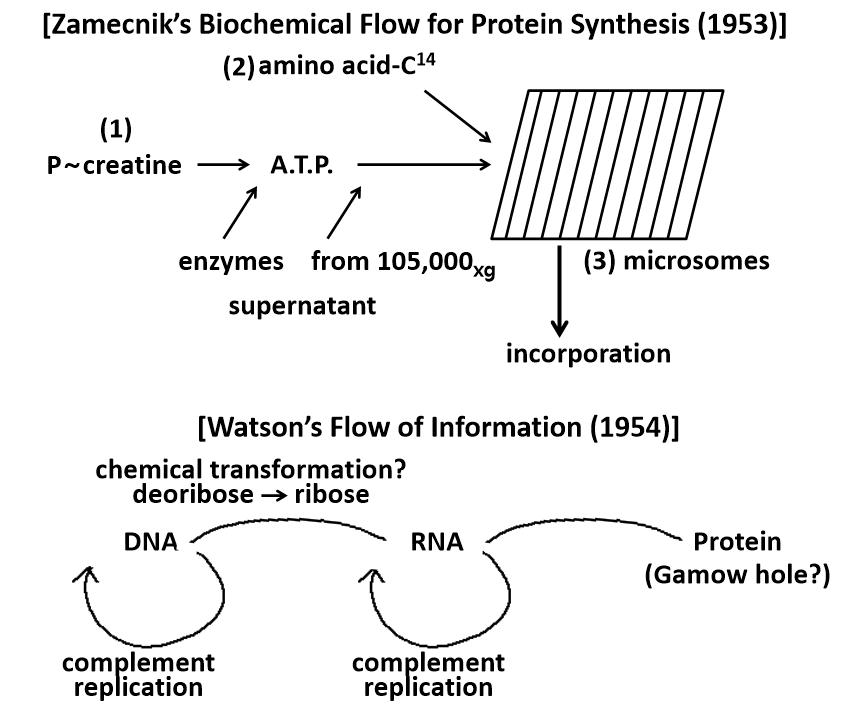
\includegraphics[width=.75\textwidth]{ART_Gim/fig.1_zamecnik_watson_bw.png}%
 \end{center}%
 \caption{Zamecnik and Watson's diagrams
 %\label{ref:RNDLYUtprlk80}(Judson, 2013, p.273)
 \parencite[based on][p.273]{judson_eighth_2013}}\label{gim.fig1}
\end{figure}

\begin{figure}[H]
 \begin{center}
 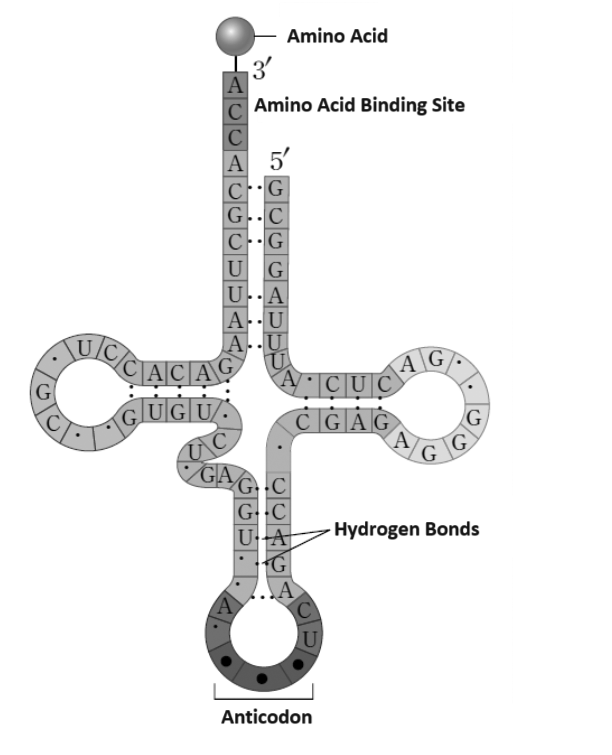
\includegraphics[width=.52\textwidth]{ART_Gim/fig.2_tRNA_bw.png}%
 \end{center}%
 \caption{The two-dimensional representations of tRNA
 %\label{ref:RND105yKmHiMv}(Holley et al., 1965, p.1464)
 \parencite[based on][p.1464]{holley_structure_1965}}\label{gim.fig2}
\end{figure}

\begin{figure}[H]
 \begin{center}
 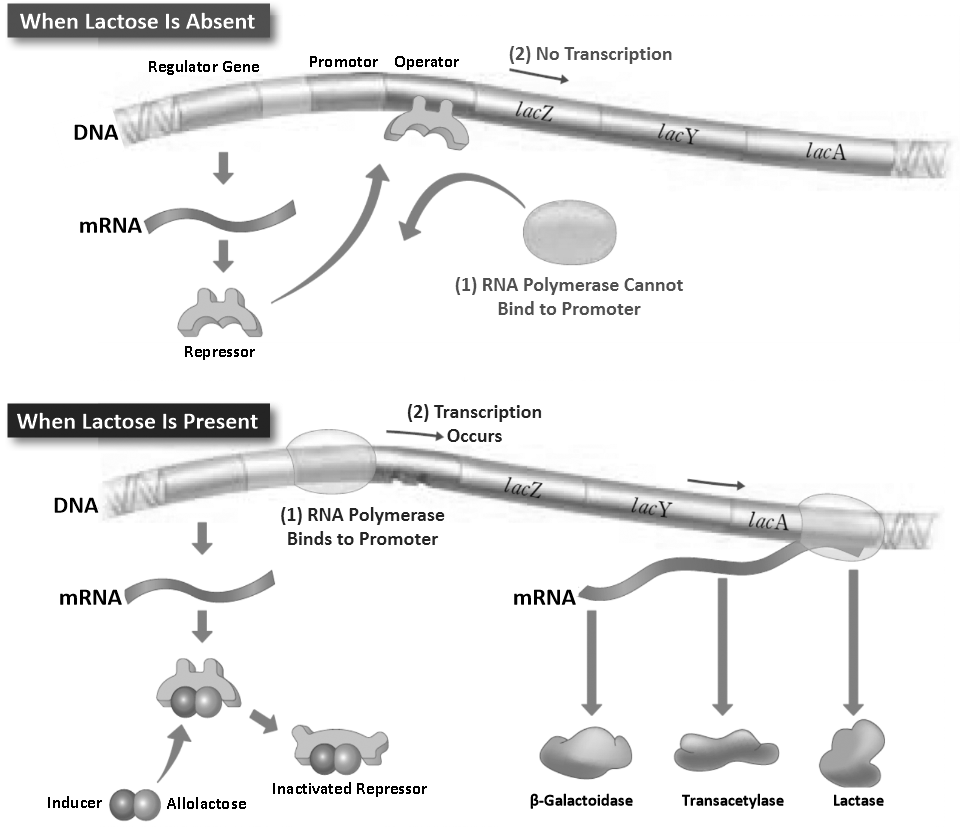
\includegraphics[width=\textwidth]{ART_Gim/fig.3_repressor_bw.png}%
 \end{center}%
 \caption[Models of the regulation of protein synthesis (based on Jacob and Monod, 1961, p.344)]{Models of the regulation of protein synthesis
 %\label{ref:RNDmyRLd6z9DD}(Jacob and Monod, 1961, p.344)
 \parencite[based on][p.344]{jacob_genetic_1961}\footnotemark\label{gim.fig3}
 }
\end{figure}
 \footnotetext{The regulation of gene expression in prokaryotes transpires at the transcriptional step. Multiple genes with analogous functions may be conglomerated into a singular transcriptional unit, thereby co-regulating their expression. This collective entity is denoted as an \textit{operon}, comprising a promoter, an operator region, and structural genes. The promoter serves as the site where RNA polymerase binds, initiating the transcription process. Simultaneously, the operator region, where a repressor protein is implicated in the regulation of transcription, spatially overlaps with the promoter, impeding RNA polymerase binding when the repressor protein is present. The structural genes encapsulate information pertaining to the proteins of three enzymes---$\beta $-galactosidase, transacetylase, and lactase---indispensable for lactose utilization. These three enzyme genes are collectively regulated within a singular operon, commonly known as the lactose operon. Expression of the lactose operon remains quiescent in the absence of lactose as a carbon source. Furthermore, even in the presence of lactose, expression ensues solely when a more favorable carbon source, such as glucose, is unavailable. The regulatory process unfolds sequentially: (1) In the absence of lactose, a repressor protein binds to the operator region, impeding transcription within the lactose operon. (2) Conversely, in the presence of lactose, the lactose inducer, allolactose, binds to the repressor protein, instigating a conformational alteration that precludes its binding to the operator region, thereby facilitating transcription within the lactose operon
 \parencite[for more details see][]{jacob_genetic_1961}.}
 
\begin{figure}[H]
 \begin{center}
 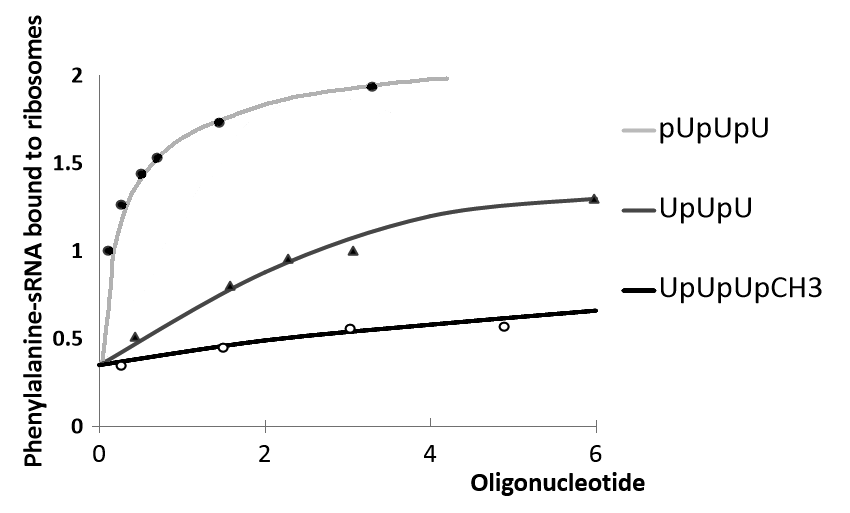
\includegraphics[width=.8\textwidth]{ART_Gim/fig.4_polyU_new_bw.png}%
 \end{center}%
 \caption{Effect of poly-U nucleotides with terminal phosphate on activities of synthesizing Phenylalanine
 %\label{ref:RND3bJIdkkvdG}(Rottman and Nirenberg, 1966, p.562)
 \parencite[based on][p.562]{rottman_rna_1966}}\label{gim.fig4}
\end{figure}


After determining the phenomenon to be explained, researchers hypothesize what objects are relevant to the phenomenon. They either formulate hypotheses about the relations between candidate objects or conduct experiments to identify whether the phenomenon occurs due to chemical interactions between objects. Watson, in 1954, and Crick, in 1958, proposed the RNA template hypothesis between DNA and protein based on existing results at that time. Zamecnik conjectured that a~ribonucleoprotein particle, later named a~‘ribosome,' within the microsome is engaged with protein synthesis
%\label{ref:RNDE4BJ8THx2q}(Hoagland et al., 1958).
\parencite[][]{hoagland_soluble_1958}. %
 The most famous experiment in molecular biology, the so-called PaJaMo experiment, performed by Arthur Pardee, Jacob, and Monod 
%\label{ref:RNDXG0NC4F3Pv}(1959),
\parencite*[][]{pardee_genetic_1959}, %
 implies DNA itself is not a~direct template of protein synthesis. Other biologists, including Severo Ochoa, Marshall Nirenberg, and Har Gobind Khorana, contributed to explaining how genetic information is transferred from one molecule to another.\footnote{Ochoa was a~Nobel Prize winner in 1959 for their discovery of the mechanisms in the biological synthesis of ribonucleic acid. Nirenberg and Khorana were also Nobel Prize winners in 1968 for their interpretation of the genetic code and its function in protein synthesis.}

Those theoretical or experimental results play a~crucial role in explaining the phenomenon of protein formation in distinct ways. Watson and Crick's RNA template hypothesis represents the genetic flow from DNA to protein via messenger RNA. This hypothesis is instrumental in explaining how DNA's genetic information is transferred to proteins. Zamecnik's diagram delineates the biochemical flow for protein synthesis utilizing the formation of ATP. This diagram proves useful in explaining the energetic components required in protein synthesis (see Fig. \ref{gim.fig1}). Holley's two-dimensional scheme from 1965 represents the structural shape of alanine RNA. This schematic representation is valuable in explaining how free amino acids are transported into the formation of polypeptides (see Fig. \ref{gim.fig2}). Jacob and Monod's models from 1961 illustrating the regulation of protein synthesis represent the interaction between regulator, operator, and structural genes. These models are effective tools in explaining how different genes contribute to synthesizing transcribed RNA (see Fig. \ref{gim.fig3}). Nirenberg's model of data shows that 5'-terminal phosphate poly-uracil sequences are more active in synthesizing phenylalanine linkages than in other sequence cases. This model is utilized to explain the structural features of mRNA required to form polypeptide linkages (see Fig. \ref{gim.fig4}).

It's important to note that researchers characterize the phenomenon of protein synthesis based on their individual interests. Molecular biologists, for instance, concentrate on genetic mappings from DNA to protein, while biochemists explore different facets of the phenomenon, such as energetic aspects (Zamecnik), structural analysis (Holley), enzymatic processes (Ochoa, Jacob \& Monod), and reaction rates (Nirenberg). Their research interests guide the representation of relevant parts of the protein synthesis mechanism. Watson and Crick, for example, speculated on the existence of messenger RNA between DNA and protein, while other biochemists employed various experimental instruments and interpreted data models. Some outcomes represent temporal steps of the mechanism, while others focus on the structural features of specific components. These diverse results prove valuable in explaining how proteins are formed in a~cell. In essence, most representations serve as worthy explanans for mechanistic explanations when used to depict the physical features of candidate parts, revealing their structural shape and considering them as relevant components. In a~nutshell, ``A researcher \textit{uses} linguistic and diagrammatic \textit{representations} of relevant parts and their organizational features of a~\textit{mechanism} to \textit{explain} a~phenomenon depending on the researcher's interests.''

Certainly, it is crucial to closely identify the relevant parts and their organizational features that are intricately linked to the occurrence of the explanandum phenomenon. However, the judgments regarding whether certain parts or organizational features are pertinent to the occurrence of the explanandum phenomenon are not issues within the conceptual dimension of explanation but rather fall under the relational dimension of explanatoriness. Here, I~emphasize that explaining a~phenomenon is conceptually identical to representing something that produces the phenomenon, and that representations are not binary but tertiary relations involving linguistic or non-linguistic representations, target entities or their organizations in the world, and human agents. These two emphases form the foundation for subsequent discussions about the relational and normative dimensions of the ontic-epistemic debates.

\section{On the explanatoriness of mechanistic explanation: Sufficiency vs. necessity}
As noted, Salmon has led us to consider mechanistic explanation as an alternative to Hempel's covering law model, presenting it as the ontic conception of explanation, in contrast to the epistemically inferential nature of the latter. In the original ontic-epistemic debate, it is well-known that Hempel's model faces numerous counterexamples, as detailed in Section 2. Consequently, many proponents of the New Mechanism, including Bechtel, argue that mechanistic explanation naturally falls into the ontic realm within the relational dimension of explanation.

However, caution is warranted because the prioritization of the ontic conception of explanation against Hempel's viewpoint is situated within the dimension of explanatoriness. I~previously underscored the importance of representation in understanding the nature of explanation within the conceptual dimension. Herein, several questions arise. If we adopt an epistemic position in the conceptual dimension of the nature of explanation, are we compelled to align with Hempel's viewpoint in the dimension of explanatoriness once again? If not, does that imply a~rejection of Hempel's ideas? Suppose we choose not to adhere to Hempel's inferential version of the epistemic account of explanatoriness. How can we maintain a~non-ontic position of explanation within the dimension of explanatoriness? Furthermore, how compatible are the two epistemic positions in the two dimensions---explanatoriness and the nature of explanation---with each other?

One of the most fatal shortcomings in Hempel's model is that his conditions for scientific explanation are insufficient in the relational dimension of explanatoriness. For instance, the flagpole or eclipse case serves as a~counterexample to the condition of the explanatory form, which is an argument. The barometer case functions as a~counterexample to the condition of the explanatory force, whether it be universal or probabilistic laws. The contraceptive pill case serves as a~counterexample to the explanatory relevance condition, which is a~logical necessity. Similarly, the vitamin C~case is a~counterexample to the condition of explanatory relevance based on high probability. These counterexamples demonstrate that arguments, laws of nature, logical necessity, and high probability alone are insufficient for scientific explanations. I~pursue a~way to adopt the epistemic position of \textit{mechanistic} explanation in the relational dimension without falling into the swamp that Hempel's model confronted.

My primary strategy to advocate the epistemic view of mechanistic explanation does not involve searching for other ideal conditions of scientific \textit{explanation}, as Hempel did. Instead, I~will regard Hempel's covering law model as a~pursuit of \textit{necessary} conditions for scientific \textit{representation}, assuming that mechanistic explanations are representations relative to pragmatic interests. In other words, Hempel's four conditions are necessary for the format of representations of mechanisms in the context of ``An \textit{agent} uses \textit{linguistic representations} to depict \textit{mechanisms} to \textit{explain} the explanandum-phenomenon.'' If some descriptions of a~mechanism fail to satisfy Hempel's conditions, then the linguistic representations of the mechanism are also deemed inadequate.

Let me begin with a~question: Are all linguistic representations, such as statements, propositions, and descriptions, inadequate for depicting mechanisms? Bechtel and Abrahamsen
%\label{ref:RNDI3rRLl63MZ}(2005)
\parencite*[][]{bechtel_explanation_2005} %
 seem to prioritize non-linguistic representations of mechanistic explanations. However, I~do not intend to discuss the priority of representational forms here. Instead, I~presume that linguistic and diagrammatic representations are equally essential modes of mechanistic explanation. Although many mechanistic explanations are diagrammatic, they never completely replace all linguistic expressions. Instead, linguistic descriptions support us in illustrating spatiotemporal processes of mechanisms, understanding detailed information, and communicating with diagrams. Most philosophers of science who advocate the New Mechanism believe that diagrammatic representations are primary modes of mechanistic models. Still, I~will concentrate on linguistic representations of mechanisms.

\subsection{Validity as a~necessary condition of linguistic representations}

As to the first condition about explanatory form, I~suggest adopting Hempel's first condition for linguistic representations of mechanisms, not for qualifying or eligible provisos of scientific explanation. I~never intend to advocate Hempel's model as an account of scientific explanation. I~am in alliance with the mainstream to criticize Hempel's covering law model. However, I~will deal with Hempel's conditions of \textit{linguistic representations} to satisfy them. My starting point was the dimension of the nature of mechanistic explanation. If we seriously take the epistemic conception of the nature of mechanistic explanation being representations, I~think Hempel's conditions help satisfy the necessary conditions for linguistic statements. In other words, all statements must be true, and an argument must be deductively valid.

In the case of protein synthesis, the ontic theorists may believe that facts, including transcription from DNA to mRNA and subsequent translation from mRNA to protein, explain how a~protein is synthesized from genetic materials. However, there seems to be a~wide gap between the belief that an actual mechanism exists and the observational evidence needed to justify that belief. No biologists directly observe the entire process from DNA to protein via mRNA. Strictly speaking, the mechanism of protein synthesis is unobservable. All processes of protein synthesis are inevitably decomposed and discovered separately in different laboratories. The results of experiments conducted on protein synthesis in each laboratory can be briefly summarized \textit{verbally}. For instance, Roger Kornberg observed a~specific case of transcription: an RNA polymerase synthesizes an mRNA sequence from DNA in a~eukaryotic cell. Marshall Nirenberg and Heinrich Matthaei observed a~particular case of translation such that a~typical complex of ribosomes and additional components synthesizes a~polypeptide containing only phenylalanine from a~poly-uracil sequence that is artificially composed by sole uracil. We can abstractly imagine that Kornberg's mRNA and Nirenberg's poly-uracil sequence are theoretically equivalent because both are a~single strand of nucleotide synthesized by an RNA polymerase in principle within a~typical environment. Under this theoretical condition, the two observations can be integrated into a~productively continuous process from DNA to protein via mRNA. Of course, diagrammatic representations are more intuitive to figure out detailed occurrences within both processes, but linguistic expressions are also possible as follows:

\begin{itemize}
    \item[\textit{C}\textit{\textsubscript{1}}.] Macromolecules, including DNA, mRNA, and protein, exist in a~eukaryotic cell.
    \item[\textit{C}\textit{\textsubscript{2}}.] Enzymes, including RNA polymerase and a~complex of ribosomes, also exist in eukaryotic cells.
    \item[\textit{P}\textit{\textsubscript{1}}.] An RNA polymerase synthesizes a~single nucleotide (mRNA) strand from DNA.
    \item[\textit{P}\textit{\textsubscript{2}}.] A~complex of ribosomes synthesizes a~primary sequence of proteins from mRNA.
    \item[\textit{C}\textit{\textsubscript{3}}.] mRNA's physical properties are always invariant, independent of concrete syntheses.
    \item[\textit{C}\textit{\textsubscript{4}}.] A~transcribed mRNA is abstractly identical to a~template of translation in principle.
    \item[\textit{E}.] The product of proteins is produced from DNA via mRNA.
\end{itemize}


The two conditions C\textsubscript{1} and C\textsubscript{2} are true on the ground that Watson \& Crick's model of DNA, Wilkins \& Franklin's X-ray diffraction evidence, and Kornberg \& Nirenberg's experimental models. Crick's central dogma, DNA $\to$ mRNA $\to$ Protein, is filled with objects. The two premises, \textit{P}\textit{\textsubscript{1}} and \textit{P}\textit{\textsubscript{2}}, are also true in Kornberg and Nirenberg's research. That is, arrows in Crick's central dogma are filled with enzymes. The additional conditions, \textit{C}\textit{\textsubscript{3}} and \textit{C}\textit{\textsubscript{4}}, are essential to integrate separate transcription and translation. These additional conditions are not ontic but epistemic claims because they are based on abstractly regular patterns from empirical research findings. Without direct observations of the mechanism of protein synthesis, the explanandum-phenomenon, \textit{E}, is a~deductive consequence of initial conditions and premises. In other words, a~deductive structure between statements is essential for linguistic representations to be useful in explaining phenomena.

Note that the mechanistic explanation above is linguistic. Premises are expressed lawfully and include empirical contents. All statements must be true either empirically or in principle. Due to two conditions \textit{C}\textit{\textsubscript{3}} and \textit{C}\textit{\textsubscript{4}}, the conclusion, \textit{E}, can be derived from \textit{C}\textit{\textsubscript{1}}, \textit{C}\textit{\textsubscript{2}}, \textit{P}\textit{\textsubscript{1}}, and \textit{P}\textit{\textsubscript{2}}. Be cautious that I~never argue that the mechanistic explanation satisfies Hempel's covering law model. I~intend to show that mechanistic explanation can be expressed linguistically as well as diagrammatically, and that if expressed linguistically, it must suffice Hempel's condition of explanatory form. Validity is a~fundamental requirement of linguistic representations to be an argument. I~never deal with valid arguments as a~sufficient condition of scientific explanation. My focus is not on finding sufficient conditions of scientific explanation but on finding the necessary conditions of linguistic representations. In other words, Hempel's logical condition is a~\textit{necessary} \textit{instruction} of linguistic representations, not a~scientific explanation. If linguistic representations are not valid, then they are absurd and non-informative in the end.

\subsection{Laws as a~necessary condition of understanding for explanatory force}

The ontic theorists claim that universal laws (or highly probabilistic laws) are insufficient conditions for scientific explanation. I~agree. However, I~emphasize that laws of nature are \textit{necessary} to understand how activities (or component operations) are engaged with entities (or component parts) and how they are spatiotemporally organized.

According to the ontic view, only things and facts are explanatory. In the case of protein synthesis, DNA, mRNA, and proteins are relevant entities. Moreover, transcription from DNA to mRNA means that the genetic information of DNA is transmitted into that of mRNA. Translation from mRNA to protein is also a~factual process that determines the types of amino acids and their order based on the genetic information of mRNA. In Crick's central dogma, all pertinent objects (DNA, mRNA, protein) are discovered, and two sequential transitions are also identified empirically. A~question arises: Can we understand, with only those objective facts, how entities act in reactions, how activities occur, and how components are organized?

Most advocates of the New Mechanism, whether they are ontic or epistemic, believe that activities (or component operations) give explanatory forces. According to Machamer, Darden, and Craver
%\label{ref:RND81P1djvH39}(2000, p.14),
\parencite*[][p.14]{machamer_thinking_2000}, %
 there are four types of activities: (i) geometrical-mechanical, (ii) electro-chemical, (iii) energetic, and (iv) electromagnetic. I~will classify such activities in Table \ref{gim.tab1}.


\begin{table}[]
\resizebox{\textwidth}{!}{%
\begin{tabular}{@{}ll@{}}
\rowcolor[HTML]{CBCEFB} 
{\bfseries Type} &
{\bfseries Activities}\\
\rowcolor[HTML]{FFFFFF} 
Geometrical &
 Shaping\\
\rowcolor[HTML]{ECF4FF} 
Mechanical &
 Fitting, Colliding, Pushing, Pulling, Opening, Closing\\
 \rowcolor[HTML]{FFFFFF} 
 Electrical &
  Attracting, Repelling\\
 \rowcolor[HTML]{ECF4FF} 
 Chemical &
  Bonding, Breaking\\
  \rowcolor[HTML]{FFFFFF} 
   Energetic &
    Thermodynamic\\
   \rowcolor[HTML]{ECF4FF} 
   Electro-magnetic &
    Electrically Conducting\\
%PP \bottomrule
\end{tabular}%
}
\caption{Types of activities.}
\label{gim.tab1}
\end{table}

\begin{figure}[H]
 \begin{center}
 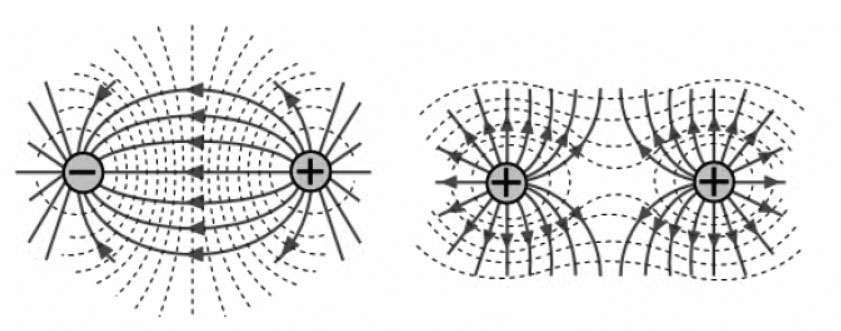
\includegraphics[width=.8\textwidth]{ART_Gim/fig.5300.jpg}%
 \end{center}%
 \caption{Attracting and repelling}\label{gim.fig5}
\end{figure}


As noted in Table \ref{gim.tab1}, activities are referred to as metaphorical terms. However, I~think that metaphorical terms are not fundamental foundations for providing explanatory forces because they must be elucidated under lower-level scientific theories. I~suggest metaphorical terms gain explanatory grounds when anchored in scientific facts, laws, or theories.

For example, electrical terms are based on Coulomb's law.\footnote{The potential energy, $\overrightarrow E(\overrightarrow r)$, of a~test charge $Q$ is the Coulombic energy of interaction between $Q$ and an arbitrary charge $q$ separated by a~distance $\overrightarrow r$ such that $\overrightarrow F(\overrightarrow r)=Q\overrightarrow E(\overrightarrow r)=Q\frac q{4\pi \varepsilon_0\overrightarrow r}$, where $\overrightarrow E(\overrightarrow r)$ is the electric force and $\varepsilon_0$ is the permittivity constant of vacuum.} Assume that atoms are the fundamental entity in our discussion.\footnote{This assumption is based on the atomic structure. All atoms consist of a~nucleus and one or more electrons. A~nucleus is electrically positive, whereas electrons are negative, so electric activities occur between them. There is attraction between the nucleus and the electrons, while there is repulsion between electrons. Repulsion also occurs between the nuclei of one atom and those of another atom adjacent to it. Electric activities are starting points to formalize entities and other activities because all materials contain a~nucleus and electrons.} Fig. \ref{gim.fig5} illustrates the explanatory ground of the electrical activities. The electrical field vector $\overrightarrow E(\overrightarrow r)$ is represented by lines pointing in the direction of the electric field at any point; that is, the electric field vector is tangent to the electric field lines at any point. The number of lines per unit area passing through a~surface perpendicular to the lines is proportional to the strength of the electric field in a~given region. For a~positive point charge, the lines radiate outward from a~point, whereas for a~negative point charge, the lines converge inward. The number of field lines leaving the positive charge equals the number of lines terminating at the negative charge. Fig. \ref{gim.fig5} illustrates the electric field lines for either two positive point charges or two negative point charges. The attraction and repulsion activities, describing the electrical interaction between charges, are mathematically formulated by Gauss' law.\footnote{The direction of electric flux is from a~positive point charge to a~negative point charge. In other words, electric flux, $\Phi _E$, is a~measure of the electric field vectors penetrating a~given surface. It is proportional to the number of field lines that pass through a~given region, $\overrightarrow A$, oriented perpendicular to the field, which is represented by the following equation: $\oint _S \overrightarrow E{\cdot}d\overrightarrow A=\Phi _E=\overrightarrow E\overrightarrow A\cos \theta $, where a~vector perpendicular to the region, $\overrightarrow A$, is at an angle $\theta $ concerning the field. The equation represents Gauss's law, ${\nabla}{\cdot}\overrightarrow E=\Phi _E=\frac Q{\varepsilon _0}$. Gauss's law implies that the electric flux through any closed surface is equal to the net charge inside the surface $Q$ divided by $\varepsilon _0$. Gauss' law is a~fundamental ground for the electrical activities.}

What about chemical activities? Those activities are also based on laws and theoretical backgrounds in physics. The two activities based on Coulomb's and Gauss's laws play a~fundamental role in constructing molecules with interactions between the nucleus and the electrons of atoms. The second step in constructing molecules is to examine the \textit{chemical} activity relating to how atoms combine in a~molecule. A~molecule comprises more than two atoms that share electrons. Covalent bonding is the most potent chemical bond when atoms share electrons. Molecular orbital theory (MO theory) is a~widely accepted theory to explain how covalent bonding occurs. Further, the Schrödinger equation can be solved analytically only for H\textsuperscript{+}\textsubscript{2}, but the solution cannot be applied to hetero-polyatomic molecules. In MO theory, the linear combination of atomic orbitals (LCAO) is an algebraic method to calculate the overall wavefunctions of electrons within a~molecule.\footnote{An atomic orbital is a~wave function that describes the behavior of an electron within an atom. Molecular orbitals can be calculated using the available atomic orbitals within various chemical contexts. (i) Electrons supplied by the atoms are accommodated in the orbitals to achieve the lowest overall energy, adhering to the constraints of the Pauli exclusion principle, which states that no more than two electrons may occupy a~single orbital, and they must be paired. (ii) If several degenerate molecular orbitals are available, electrons are added singly to each orbital before doubly occupying any one orbital because that minimizes electron-electron repulsions. (iii) Hund's rule implies that if two electrons occupy different degenerate orbitals, a~lower energy is obtained if they do so with parallel spins. In short, the structure of a~molecule is determined by the configuration of electrons within the molecules under the minimal energetic state. All these descriptions of physicochemical backgrounds are prepared with reference to Atkins and de Paula's Physical Chemistry textbooks
%\label{ref:RNDfgHGFjtinW}(see Atkins, De Paula and Friedman, 2014).
\parencite[see][]{atkins_physical_2014}.%
}

Hence, laws and theoretical backgrounds provide a~scientific understanding of why metaphorical terms are explanatory. I~do not argue that universal laws are a~sufficient condition of scientific explanation. Instead, I~emphasize the necessity of laws for an intellectually ultimate understanding of the explanandum phenomenon.

\subsection{Counterfactual inference as a~necessary condition of explanatory relevance}

Logical necessity is not a~sufficient condition for explanation. Even if an argument concludes the occurrence of a~phenomenon from sentences about relevant components and their organizational features is valid, the presence of a~sentence about an entity being causally inefficacious to the occurrence of the phenomenon in the premises renders the argument not a~mechanistic explanation. Moreover, no matter how much an inductive argument is based on high probability in the case of most prokaryotic cells, there is no guarantee that the argument will immediately apply to the case of eukaryotic cells. For this reason, Hempel's two conditions of explanatory relevance are deemed insufficient.

Assuming that explanations are representations, I~emphasize that Hempel's conditions should be considered necessary but insufficient. As noted earlier, logical necessity is crucial when explaining a~phenomenon through a~set of linguistic descriptions. It serves as a~prerequisite for the explanatory form rather than a~condition guaranteeing explanatory relevance. Within Hempel's account of explanation, there are no adequate conditions for mechanistic explanation.

Alternatively, I~introduce an inference to affirm the relationship of constitutive relevance between the explanandum phenomenon and descriptions of parts and organizational features: \textit{counterfactual conditional}.\footnote{In most cases of biological mechanisms, descriptions of the explanandum phenomenon are at a~higher level than descriptions of component parts and their activities. Advocates of the New Mechanism, particularly Craver, regard explanatory relevance in mechanistic explanation as \textit{constitutive} relevance. Although the philosophical debate remains, we will tentatively assume here that the two concepts of relevance are identical.} All phenomena to be ontologically explained depend on their lower-level mechanisms. This ontological dependence can be linguistically reformulated by a~‘because' complex sentence. To ensure explanatory relevance in the relational dimension, it must be demonstrated that the statement ‘The description of the phenomenon clause (P) is true because a~set of descriptions of mechanism clauses (M) is true.' The truth conditions of this sentence are provided by the counterfactual condition, stating that ‘P-clause because M-clauses' is true if and only if: (i) ‘P-clause' is true, (ii) all ‘M-clauses' are true, and (iii) ‘If it were not the case that M, it would not be the case that P' is true.\footnote{This kind of formal investigation of the explanatory relationship based on the ‘because' complex sentence has been slightly shown in Wright and Bechtel's paper in 2006. However, they did not formulate their idea at all. I~will adopt the counterfactual truth conditions of the ‘because' sentence as an epistemic condition of counterfactual inference for explanatory relevance. They said, ``Descriptions of mechanisms are not just coincident with, or derivative from, explanations---they \textit{are} explanations. But explanations are not merely lists of descriptions of mechanisms or sets thereof: they include inferential and simulatory operations on them. (Considerations of the semantics of the explanatory connective ‘because,' as well as what it is that arrow in box-and-arrow diagrams represent, help in grasping this point.)''
%\label{ref:RND0o2wh99B14}(Wright and Bechtel, 2007, p.53, emphasis original).
\parencite[][emphasis original]{wright_mechanisms_2007}. %
 I~will develop their basic idea by pursuing counterfactual conditions of the ‘because' sentence.}

A~sentence ‘P because M' indicates the explanatory relevance of mechanistic explanation between the explanandum phenomenon and explanans, assuming that every phenomenon (P-clause) depends on its mechanisms (M-clauses). Suppose a~description within the P-clause is false. In that case, all claims of explanatory relevance are false, as the first condition is not satisfied, regardless of the truth of the descriptions of mechanisms. It highlights that characterizing the explanandum phenomenon by determining its initial and terminal conditions is the primary cognitive activity of explanation. Similarly, if a~description within the mechanism clauses is false, the ‘because' sentence also becomes false, as the second condition is not satisfied, irrespective of the truth of the phenomenon description. These considerations presuppose that mechanistic explanation is a~cognitive activity in the first conceptual dimension of explanation. It is important to note that some explanations can be false due to misrepresentations, not the non-existence of relevant components and their organizational features.

The third truth condition is crucial in judging the relevance between P~and M~descriptions. Let's assume that M~is a~description of a~candidate for the relevant part of a~mechanism. If the occurrence of the P-description is observed even when it is not the case that M~(that is, $\sim$M), then it is certain that the referent in M~is irrelevant. The counterfactual conditional ``If it were not M, it would have been P'' is false since the P-description is true even if the M-description is false. For instance, from the molecular biologists' perspective, let me first discuss a~linguistic description of M-clause: ``X is a~genetic intermediate between DNA and protein'' (M\textsubscript{1}). Suppose a~biologist makes M\textsubscript{1} by filling the description with ribosomal RNA within a~microsome. In that case, ribosomal RNA is not relevant because it has been proven that protein synthesis occurs even if M\textsubscript{1} is false. On the other hand, suppose another biologist makes M\textsubscript{1} by filling the description with messenger RNA. In this case, the counterfactual conditional ``If it were not M\textsubscript{1}, it would have been not P'' is true since protein synthesis cannot be realized without mRNA.

It should be noted that we are not suggesting here that ribosomal RNA is an entirely incorrect component in protein synthesis. Rahter, we found that ribosomal RNA was not an appropriate referent in the mechanistic description, ``\textit{X} is a~genetic intermediate between DNA and protein.'' Ribosomal RNA is the correct referent for other mechanistic descriptions, such as ``\textit{X} synthesizes polypeptides based on messenger RNA sequence'' (M\textsubscript{2}). In other words, it is not realistic to determine whether a~single referent is correct or incorrect for an entire mechanism. A~referent may be correct for a~description in one context and may be incorrect for other descriptions in another context.\footnote{Reversely, the occurrence of the P-description may not be observed even if a~mechanism description is true. In this case, the counterfactual condition ``If it were M, it would have been $\sim$P'' is false so that the mechanism description includes irrelevant information. Here, all true mechanism descriptions can be proven as totally irrelevant to the phenomenon because all referents and their properties in M-clauses never contribute to generate the occurrence of the phenomenon. As a~result, we easily ignore all such mechanism descriptions.}

Additionally, from the biochemists' point of view, let me focus on enzymatic activities, particularly RNA polymerase. The counterfactual inference is well applicable to cases of step-by-step processes. An RNA polymerase is a~key entity synthesizing mRNA with DNA. When explaining the production of mRNA, ontic theorists may provide a~mechanistic explanation as follows. Suppose that an explanandum-phenomenon, \textit{P}, is the production of mRNA sequence through transcription. The emergence of mRNA is the terminal outcome of the mechanism of RNA synthesis. The initial condition of the production is nothing of any ribonucleic acids in a~cell's nucleus. However, we must assume that there are a~lot of building units of the mRNA, including adenine, uracil, guanine, and cytosine. A~M-clause is ``mRNA sequence emerges in a~cell's nucleus.'' The truth condition of the M-clause could be determined by empirical manipulation like centrifugal identification. In the 1960s, the existence of mRNA was proven by Brenner et al. What are the M-clauses as explanans of the P-clause? Briefly speaking, there are five statements of the M-clauses as follows:

\begin{itemize}
    \item[M\textsubscript{3}.] An RNA polymerase attaches a~DNA region called the promoter sequence.
    \item[M\textsubscript{4}.] The RNA polymerase unwinds the two strands of DNA.
    \item[M\textsubscript{5}.] The RNA polymerase moves along the DNA.
    \item[M\textsubscript{6}.] At that time, the RNA polymerase synthesizes individual RNA nucleotides to the growing mRNA strand based on a~single strand of DNA template.
    \item[M\textsubscript{7}.] The RNA polymerase detaches from the DNA template when stopping the synthesis.
\end{itemize}
\enlargethispage{1.5\baselineskip}


If M\textsubscript{6} is not true, the P-description, ``A transcription is generated,'' may also not be true since M\textsubscript{6} implies the P-description. M\textsubscript{6}~temporally depends on M\textsubscript{5}, which also depends on M\textsubscript{4}, which depends on M\textsubscript{3}. M\textsubscript{7} indicates the end of the series from M\textsubscript{3} to M\textsubscript{6}. As a~result, if a~sequence of successive M-descriptions is false, then the P-description as a~consequence of the terminal M-description is also false. That is, if M\textsubscript{3}--M\textsubscript{7} is not true, then P~is not true, too. In conclusion, M-descriptions, M\textsubscript{3}--M\textsubscript{7}, are explanatory relevance to the P-description. An inference with the counterfactual conditional is worthy of being an adequate epistemic condition to discern whether any mechanistic descriptions are relevant to the phenomenon description.

Finally, I~do not argue the structural identity between mechanistic explanation and prediction. We do never adopt the demarcation problem because prediction is an explanatory virtue. Hempel's four conditions are insufficient for scientific explanations to satisfy but necessary to evaluate whether linguistic representations are adequate. No matter how logical necessity (or high probabilistic necessity) is satisfied from the premises and their conclusion, it does not guarantee that linguistic representations are scientific explanations. However, if all statements are employed to explain something, they must be logically consistent. If not so, independently of whether logical necessity is a~sufficient condition to determine the eligibility of scientific explanation, all linguistic representations are not informative. Moreover, laws of nature are not sufficient conditions for scientific explanations. However, in the absence of laws of nature, it is difficult to identify the explanandum phenomenon and further understand how organizational features of mechanisms contribute to producing the occurrence of the phenomenon.

Hempel's account is epistemic because epistemic inferences, such as logical calculus or derivations, establish explanatory relevance. In contrast, Salmon's causal-mechanical account is ontic because explanatory relevance is established not by mental inferences based on logic but by actual target systems in nature, expected to bring about a~phenomenon to be explained. Attempts to evade Hempel's shadow were unsuccessful in establishing the epistemic view in the relational dimension of explanatoriness in the original ontic-epistemic debate.

To advocate the epistemic conception of mechanistic explanation, I~propose two epistemic ways to illuminate the explanatory relevance between the explanandum phenomenon and its explanans: the necessity thesis of linguistic representations and the counterfactual inference. Hempel's epistemic conditions are necessary for mechanistic explanations, which are linguistic outcomes representing actual mechanisms under the assumption that linguistic descriptions express the contents of mechanistic explanation. Additionally, a~counterfactual inference of the ‘because' sentence helps check whether the relation between the explanandum and explanans is relevant. I~illustrate this with molecular and biochemical cases. These alternative interpretations of Hempel's account of explanation in the relational dimension of explanatoriness are based on the previous consequence that the nature of explanation is a~cognitive activity in the conceptual dimension.

\section{On the norms of mechanistic explanation: Completeness vs. purpose-dependence}
\enlargethispage{1.5\baselineskip}
Most philosophers have discussed the normative dimension by emphasizing the superiority or interaction between ontic and epistemic norms
%\label{ref:RND0BmXWK6A6a}(Kaplan and Craver, 2011; Illari, 2013; van Eck, 2015; Sheredos, 2016).
\parencites[][]{kaplan_explanatory_2011}[][]{illari_mechanistic_2013}[][]{van_eck_reconciling_2015}[][]{sheredos_re-reconciling_2016}. %
 In contrast, I~will focus in this Section on these two types of norms as criteria for evaluating mechanistic explanations. Many ontic theorists defend ontic norms by mentioning that ontic norms are the most powerful standard for evaluating explanations 
%\label{ref:RNDn576ysYLyz}(see Craver, 2014; Povich, 2018).
\parencites[see][]{kaiser_ontic_2014}[][]{povich_minimal_2018}. %
 Participating in the ontic-epistemic debate as a~standard for evaluating mechanism explanations is noteworthy since it is an issue of the normative dimension of explanation that has yet to receive much attention among epistemic advocates. However, I~would like to point out that, contrary to the wishes of ontic theorists, when they use ontic norms when evaluating mechanistic explanations, they encounter dilemmas that run counter to our common sense.

\subsection{Pessimistic induction and demarcation of explanation}

If we adopt the idea that mechanistic explanation is a~cognitive achievement to represent a~mechanism linguistically or diagrammatically in the conceptual dimension, what implications does it have for normative issues? Generally, mechanists refer to representations of mechanisms as mechanism schemes. Assuming this equivalence of abstract two terms, we can say that Craver emphasizes two ontic norms of mechanistic explanation: (i) completeness and (ii) correctness. He, with Darden, defines the two terms as critical criteria to evaluate mechanism schemes
%\label{ref:RNDeBt3Hf36sc}(Craver and Darden, 2013, p.9):
\parencite[][p.9]{craver_search_2013}: %
 ``Completeness presumes that there is a~complete target mechanism in the world, and one can assess the extent to which the schema includes all and only the entities, activities, and organizational features in the target. Correctness presumes that there is a~fully instantiated target mechanism in the world, and one can assess the degree of fit or mapping between items in the scheme and items in the target mechanism.'' As noted previously, completeness is a~chief ontic goal of mechanistic explanation. Correctness is closely related to Craver \& Kaplan's 3M requirement between a~scheme and its target mechanism.

Note that most ontic theorists, including Craver, Kaplan, and Povich, further employ those ontic norms to demarcate good from bad explanations. Ontic theorists seem to believe that a~philosophical search for any criteria to evaluate the quality of explanation is a~critical task of the philosophers of science. They think of mechanism sketches (or how-possibly models) as mere conjectures of the target. On the other hand, they appear confident that we can attain correct and complete representations of the entire target mechanism as how-actually models. They tend to regard mathematical descriptions of natural patterns as trifling or partial explanations. Hodgkin and Huxley's equations of action potential are the typical case. No matter how the equations allude to regular patterns across a~membrane of a~neuron quantitively, ontic theorists underestimate the explanatory values of mathematical descriptions
%\label{ref:RNDeGOFEod5W7}(see Craver, 2007).
\parencite[see][]{craver_explaining_2007}. %
 They stress the significance of only qualitative descriptions (or diagrams) with causal terms within Table \ref{gim.tab1}. They seem to believe that referring to relevant components and their organizational patterns is the superior prerequisite of mechanistic explanation than depicting them mathematically.

\enlargethispage{1.5\baselineskip}
Let's delve into ontic norms by addressing the following questions: Is the ontic norm of completeness attainable? How can we determine whether completeness is achieved without prior knowledge of the target mechanism? These inquiries pose metaphysical doubts about ontic norms. Moreover, most mechanism schemes are inevitably labeled as bad explanations when completeness is employed as a~criterion for evaluation. The question then arises: Should we rely on completeness to distinguish between good and bad explanations?

Firstly, is the ontic norm of completeness applicable to the evaluation of hypothetical mechanism schemes? According to Craver \& Darden's definition of completeness, an agent must possess complete information about a~target mechanism before employing this ontic norm. This comprehensive information includes the types of entities, activities, and their organizational features. However, completeness is an unattainable criterion when applied to practical contexts. Information about the target must be known in advance to use the completeness norm in evaluation. Yet, as demonstrated earlier, direct access to a~target mechanism is not feasible. We cannot grasp information about mechanisms all at once, and scientific instruments do not aid in perceiving the entire process of the explanandum phenomenon. Instead, we must partially grasp mosaic information about the mechanism and then piece the information together.\footnote{Craver emphasizes the mosaic unity in neuroscience for a~different reason
%\label{ref:RNDpnY1dXT2yg}(see Craver, 2007).
\parencite[see][]{craver_explaining_2007}. %
 He argues that mechanistic explanations in neuroscience are not reduced to the fundamental level but are unified by multilevel results of different fields.} Completeness is not a~tangible concept that can be achieved in one fell swoop. Instead, it is a~variable concept that gradually changes in magnitude and degree as the obtained evidence increases.

Second, completeness is not an appropriate criterion for evaluating whether an explanatory representation is good or bad. This ontic constraint is a~variable concept depending on how far the research has progressed. Is Crick's central dogma, DNA $\to$ RNA $\to$ Protein, a~mechanism scheme? Most ontic theorists seem to answer yes because the missing link was filled with RNA. Further, this scheme opens the way to explain how proteins are synthesized from DNA. However, this mechanism scheme seems to be a~bad explanation under the completeness criterion because the scheme does not include which enzymes act when RNA is transcribed from DNA and when protein is translated from RNA. Perhaps ontic theorists believe a~complete explanation can be achieved by enumerating the complex processes by which RNA and protein are synthesized separately, using causal terms. Or they may believe that a~complete explanation can be more easily achieved if the two syntheses are presented concisely, using diagrams.

Perhaps ontic theorists would say this is on the way to complete a~mechanism description. Of course, pursuing completeness by adding unknown sub-processes in more detail than the previous mechanism descriptions is not problematic. The genuine problem arises from the fact that proposing a~mechanistic explanation depends on additional research findings. More novel components will be continuously discovered in pursuit of a~complete mechanism description. And new interactions between the components will also emerge. The additional achievements of these discoveries are typical of biological research, which is entirely natural. But do biologists always classify their explanations as good or bad based on the yardstick of completeness? That rarely happens. All of their explanations are on a~\textit{continuum}, and it is highly unrealistic to divide the sequence of achievements into good and bad explanations solely based on completeness.

\enlargethispage{1.5\baselineskip}
Let's reconsider the case of protein synthesis, particularly examining whether the mechanism schema in Fig. \ref{gim.fig6} serves as a~complete and correct model to represent the full processes of protein synthesis. Regrettably, the schema is inherently incomplete. Firstly, the discovery of reverse transcriptase in 1970 unveiled a~reverse flow of genetic information from an RNA virus to a~DNA provirus. Secondly, eukaryotic mRNA is not immediately ready for translation. RNA at this stage is termed precursor-mRNA and must undergo additional processing before transitioning from the nucleus to the cytoplasm as mature mRNA. These processes involve RNA capping, polyadenylation, and splicing, modifying mRNA in various ways. These modifications enable a~single gene to produce more than one protein.\footnote{RNA capping modifies the 5' end of the RNA transcript, which is the end that is synthesized first. RNA is capped by the addition of an atypical nucleotide, which is a~guanine nucleotide containing a~methyl group attached to the 5' end of RNA in an unusual way. This capping occurs after RNA polymerase II has produced about 25 RNA nucleotides long before completing transcription of the entire gene. Polyadenylation provides newly transcribed mRNA with a~special structure at the 3' end. Unlike bacteria, where the 3' end of an mRNA is simply the end of a~chain synthesized by RNA polymerase, the 3' end of a~eukaryotic mRNA is first trimmed by an enzyme that cleaves the RNA chain at a~specific sequence of nucleotides. The transcript is then finished by a~second enzyme that adds a~series of repeating adenine nucleotides to the cleavage ends. These poly-A tails are typically hundreds of nucleotides long. Splicing removes introns from precursor-mRNAs. Introns are unnecessary regions for encoding proteins. The rest of the mRNA consists only of regions called exons that are needed to synthesize the protein. Editing is the process of changing some nucleotides in mRNA. For example, a~human protein called APOB, which helps transport lipids in the blood, has two different forms due to editing. One form is smaller than the other because editing adds an earlier stop signal to the mRNA. RNA editing processes such as these occur all the time in real cells. In order for the mechanism by which RNA is synthesized from DNA to meet the criteria for completeness, an explanation including these processes is required.} Third, the full mRNA sequence after transcription is not the genetic code for synthesizing proteins. Precursor RNAs synthesized by an RNA polymerase in the nucleus must be edited. Particularly, the splicing mechanism in eukaryotes is essential; non-genetic portions within the precursor RNAs, the so-called introns, must be deleted, and genetic portions, the so-called exons, must be ligated. Splicing implies that both synthesizing processes, transcription, and translation, are not the only processes within protein synthesis. In other words, Fig. \ref{gim.fig6} is never a~complete model of protein synthesis.
\enlargethispage{1.5\baselineskip}

\begin{figure}[H]
 \begin{center}
 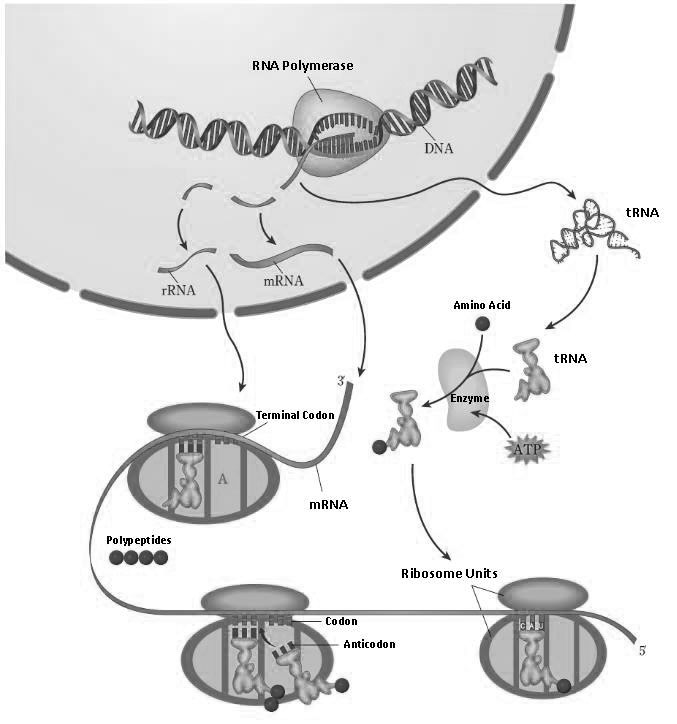
\includegraphics[width=.8\textwidth]{ART_Gim/fig.6_bw.jpg}%
 \end{center}%
 \caption{Mechanistic schema for protein synthesis
 %\label{ref:RND5ZkgEBeN2n}(Darden, 2006, p.117)
% \parencite[][p.117]{darden_reasoning_2006}
 }\label{gim.fig6}
\end{figure}

Maybe ontic theorists will complain that those two cases, retrovirus and splicing reactions, do not refute their ontic norms to evaluate mechanism schemes because they are not counterexamples but evidence of their ontic criteria. The more processes are filled with the previous scheme, the more complete and correct explanations are achieved. Suppose that it is okay to accept the ontic theorists' claim such that the mechanism scheme, including (i) Watson's central dogma, (ii) biochemists' discoveries of enzymatic reactions from DNA to protein, (iii) a~special case of genetic information flow in a~retrovirus, and (iv) splicing mechanism in eukaryotes, is the complete and correct model of protein synthesis. Regrettably, again, Ochoa's discovery misrepresents RNA synthesis because he never found RNA polymerase but polynucleotide phosphorylase. Roger Kornberg successfully analyzes the structural features of RNA polymerase and its functions in eukaryotes in the early twentieth century. In other words, all mechanistic schemes in the absence of Roger Kornberg's achievements are certainly incomplete and incorrect.

Again, ontic theorists would complain that the system of mechanisms, up to and including Roger Kornberg's discovery, is a~complete and accurate model of protein synthesis. The problem with answering this way is that ontic theorists can never seem to qualify themselves as tools for evaluating mechanism schemes other than holding their ground. Whenever a~discovery emerges, the existing mechanism scheme becomes a~false description, and a~more complete and accurate explanation is achieved. As biologists' research accumulates, situations like this will occur more frequently in the future. It is clear, then, that any mechanism scheme currently believed to be complete and correct will one day become a~bad explanation. The ontic norms applied to evaluating explanations inevitably allow for such \textit{pessimistic} prospects in situations where theory propagation is the norm. In this scenario, we must reluctantly conclude that achieving a~complete and precise mechanism is an elusive goal, both at present and in the foreseeable future.

This conclusion is analogous to the conclusion of the pessimistic induction argument against scientific realism. The pessimistic induction argument shows that if past successful and truly accepted theories were false, we fail to believe the realist's claim that our currently successful theories are true because current theories will also be false as past successful theories were confronted. Similarly, if one adopts the realistic point of view of the existence of a~mechanism and admits that mechanism schemes are continuously developed toward more complete and more correct models, then it is skeptical to attain the complete and correct model of the mechanism.

Advocates of the ontic conception of explanation believe (i) that we can one day achieve complete and accurate mechanism descriptions and (ii) we must assess mechanism schemes under the ontic norms. However, suppose the two beliefs juxtapose with each other. In that case, we are inevitably unable to obtain complete and accurate mechanism descriptions, or we are forced to brand almost all known mechanism descriptions as bad. Ontic theorists accept that mechanistic models must be developed from how-possibly to how-actually models. Mechanism sketches become just how-possibly models when acquiring more complete and correct models. By filling in intermediate components between the initial and terminal conditions, mechanism sketches must be developed into more complete and correct schemes as how-actually models. Suppose one realizes the acquisition of a~complete and correct model of the explanandum phenomenon. In that case, the how-actually model is a~good explanation, and all the early sketchy how-possibly models become bad explanations. Note that both ontic norms of completeness and correctness are criteria for evaluating mechanistic schemes from a~\textit{realistic} point of view. Craver and Darden reveal their realistic stance by saying that:

\myquote{
At the most abstract level, mechanism schemas are evaluated in terms of their depth, their completeness, and their correctness. We discuss these dimensions of evaluation and some tests for evaluating a~schema along these dimensions. Our orientation toward these questions might be described as a~\textit{garden-variety realism} moderated by a~sensible pragmatism
%\label{ref:RNDOu4WvGgjRc}(Craver and Darden, 2013, p.9, emphasis added).
\parencite[][emphasis added]{craver_search_2013}.%
}
Craver and Darden
%\label{ref:RNDyFBT8TKnwf}(2013, p.94)
\parencite*[][p.94]{craver_search_2013} %
 emphasize the close relationship between an ontic norm such as correctness and realism: ``The difference between how-possibly, how-plausibly, and how-actually a~mechanism works is a~difference in correctness. Mechanists are garden-variety realists about such things: the goal is to describe correctly enough (to model or mirror more or less accurately) the relevant aspects of the mechanism under investigation.'' It is taken for granted that ontic norms are realistic criteria because they are based on the external existence of relevant entities and activities of the target mechanisms.

A~problem of ontic norms as criteria for evaluating mechanism schemes is that all past achievements of mechanism schemes are just bad and provisional explanations. In other words, this decision is so hasty that it raises the problem of treating all existing scientific achievements as useless and bad things. But such a~judgment is too extreme. Is the discovery that genes are passed from DNA to mRNA to proteins a~bad achievement? Are all the diagrams missing the splicing process a~bad diagram of how proteins are synthesized? Are all of Roger Kornberg's schemes where RNA polymerase is not named or omitted bad descriptions? No matter how imperfect or inaccurate these achievements may ultimately be, they must be our historically significant assets. It is very questionable whether these achievements are appropriately treated as useless or bad simply because they are not complete and accurate mechanism schematics.

To summarize, ontic proponents may accept that the mechanism of protein synthesis, like the diagram of Fig. \ref{gim.fig6}, explains the production of the primary sequences of proteins in molecular biology. Is this mechanism complete? If they think this mechanism is complete, this judgment is false because the splicing mechanism is ignored. If they think this mechanism is incomplete, then ontic norms seem sterile to distinguish how-actual from how-possible models. Ontic theorists believe that ontic norms such as correctness and completeness play a~role in demarcating good from bad explanations. Unfortunately, as long as they continue to hold on to this belief, ontic theorists end up labeling a~mechanistic scheme, considered a~very important biological achievement, as a~‘bad' explanation. This tragic situation has resulted from adhering to a~particular philosophical position, the ontic criteria for evaluating mechanism schemes. Regardless of whether the splicing mechanism was discovered, Fig. \ref{gim.fig6} is still a~good representation that explains a~fairly important phenomenon in protein synthesis.

\subsection{Ontic norms as methodological instructions}

Suppose ontic norms such as completeness are difficult to achieve, and it is problematic to classify incomplete mechanism schemes into bad explanations according to these norms. What role do these norms play? Suppose we need not seriously consider mechanism schemes to be tagged as good or bad. Ontic norms can motivate researchers to provide more advanced explanations than previous explanations of mechanisms. As noted, mechanistic explanation relies on mechanistic inquiries. Completeness plays an instruction in developing existing schemes by filling unidentified processes or illuminating known entities' uncovered properties.

Again, for instance, the self-splicing mechanism in eukaryotes was discovered after most processes within the mechanism of protein synthesis were known in the 1980s. When discovering the structure of DNA in 1953, Watson and Crick never acknowledged the two distinctions, exons and introns, within nucleic acids. Exons are portions that include genetic information, whereas introns do not. So, introns must be removed before a~ribosome synthesizes proteins based on the genetic sequences of mRNA. Thomas Cech discovered the splicing mechanisms in \textit{Tetrahymena} (see Fig. \ref{gim.fig7})
%\label{ref:RNDKM1pP6CS48}(Zaug, Grabowski and Cech, 1983).
\parencite[][]{zaug_autocatalytic_1983}. %
 Due to the discovery of splicing processes, understanding of protein synthesis has increased. Moreover, Cech discovered a~new property of RNA. Until the 1980s, most biochemists believed that all enzymes are proteins. However, while investigating the splicing mechanism, Cech was also aware of the enzymatic property of RNA molecules. That is, Cech shed light on a~novel fact that biological reactions from pre-rRNA to spliced rRNA occur in the absence of enzymes (see Fig. \ref{gim.fig7}). Cech 
%\label{ref:RNDcKN42rgx2z}(1986)
\parencite*[][]{cech_model_1986} %
 proved it experimentally so that he won the Nobel Prize in 1989. Cech's discovery of ribozyme, a~compound of RNA \& enzyme, contributes to making more complete lists of referents of enzymes in the world. Cech's achievements are totally compatible with the previous outcomes. Biologists investigate their research to explain biological phenomena at the molecular level more completely. Ontic norms are methodological instructions in mechanism inquiries.\footnote{Although I~only focus on completeness here, correctness is also an important ontic norm in mechanism inquiries. Without referring to referents as correct entities in a~mechanism, we cannot explain the explanandum phenomenon successfully.}

\begin{figure}[H]
 \begin{center}
 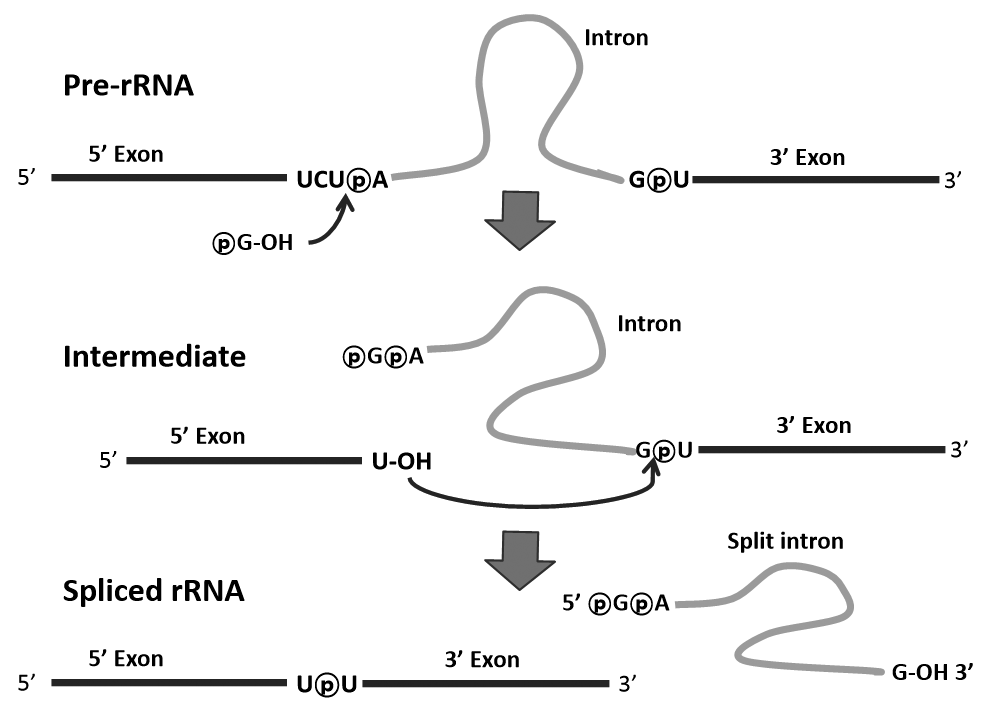
\includegraphics[width=\textwidth]{ART_Gim/fig.7_splicing_bw.png}%
 \end{center}%
 \caption{Cech's self-splicing mechanism
 %\label{ref:RNDiJ4MUJxdNH}(Zaug, Grabowski and Cech, 1983, p.582)
 \parencite[based on][p.582]{zaug_autocatalytic_1983}}\label{gim.fig7}
\end{figure}


Finally, I~would like to emphasize that whether an explanation is good or bad is not determined by any criteria but rather by its appropriateness or relevance to the topic determined in the given context. Ontic norms are instructions of mechanistic inquiries to discover patterns, not criteria to judge whether a~description is good. Ontic norms are self-contradictory because scientific achievements are thrown away as bad explanations. Completeness is an infeasible Utopian standard to be realized in science. It rather is realizable following the explainer's interests. A~philosophical distinction on explanatory normativity based on ontic norms seems a~pseudo-project.

Interestingly, Craver and Darden also agree on the pragmatic aspect of mechanistic explanation by acknowledging that ontic norms are compatible with agents' interests or given contexts by saying:

\myquote{
In speaking this way, we also intend to allow that a~schema can be complete and correct enough for the \textit{purposes} at hand without being fully complete or correct. One can acknowledge the ideals of completeness and correctness for descriptions of mechanisms while, at the same time, recognizing that science often traffics in \textit{idealized} and \textit{incomplete} schemas
%\label{ref:RNDBHgV0NHMyK}(Craver and Darden, 2013, p.9, emphasis added).
\parencite[][emphasis added]{craver_search_2013}.%
}
The pragmatic point of view was shown in the discussion of the conceptual dimension of the nature of explanation. Remind that the nature of mechanistic explanation is the tertiary relation among the representer, targets, and agent's goal in a~given context. When judging whether a~mechanistic explanation is successful, the explanation must be an adequate answer to a~question about why the explanandum phenomenon happens. According to van Fraassen
%\label{ref:RNDshKkR1q14q}(1980),
\parencite*[][]{van_fraassen_scientific_1980}, %
 an explanation is an answer to a~why-question. Here, I~do not apply van Fraassen's theory of explanation to mechanistic explanation. Still, I~emphasize that mechanistic explanations are evaluated by whether adequate representations explain the explanandum phenomenon under the agent's interest.

The same phenomenon can be explained differently depending on what aspects, to some degree, explain the phenomenon. For example, protein synthesis can be explained diversely concerning researchers' interests. Molecular biologists Watson and Crick were interested in the genetic flow from DNA to protein. The number of bases within nucleic acids is four, but the number of amino acids is twenty. So, the order of the bases in DNA determines what kinds of nucleic acids are in protein. By guessing the existence of a~single linear sequence of nucleic acids, or messenger RNA, they imagined how sequences of two or three bases correspond to 20 different types of amino acids. As a~result, the simple mechanism scheme, DNA$\to$RNA$\to$Protein, explains a~temporal order among essential entities within the mechanism. By contrast, biochemists Zamecnik and Hoagland focused on the energy flow in the form of ATP when amino acids are activated in synthesizing the peptide bond. Their chemical interest in protein synthesis led to the discovery of transfer RNA, which links the genetic code to amino acids. As a~result, Zamecnik's diagram in Fig. \ref{gim.fig1} explains how biomolecules interact with each other to synthesize the peptide bond.

Further, another biochemist, Cech, was interested in what enzymes mediate the splicing reactions of precursor ribosomal RNA before mRNA moves out of a~nucleus to synthesize protein. As a~result, Cech's diagram in Fig. \ref{gim.fig7} explains how splicing reactions, including cleavage of pre-rRNA, ligation, and cyclization, occur without enzymatic proteins. Besides them, numerous molecular biologists and biochemists have proposed models representing various aspects of the protein synthesis process, depending on their respective fields of interest. For the same protein synthesis process, molecular biologists focus on genetic information, and biochemists focus on energy equivalence. Even among the same biochemists, someone discovers the energy components needed for chemical reactions, and someone else discovers new functions of RNA. Likewise, the topic, scope, and purpose of explaining the protein synthesis process vary depending on the researcher's interests. The important thing is that all of them are significant achievements in biological sciences, even if each incompletely explains the full processes of protein synthesis. Whether a~mechanistic explanation is good or not depends upon the issue of \textit{how much an answer to the question is attained}.

As noted, Craver, Bechtel, and Wright adopt Salmon's distinction between ontic and epistemic. However, they disagree about the nature of mechanistic explanations. Craver
%\label{ref:RNDXpKAIeFKK5}(2006; 2007; 2014)
\parencites*[][]{craver_when_2006}[][]{craver_explaining_2007}[][]{kaiser_ontic_2014} %
 argues that the mechanistic explanation is also ontic, whereas Bechtel and Wright 
%\label{ref:RNDVFMWcu7K3P}(Wright and Bechtel, 2007; Wright, 2012; 2015)
\parencites[][]{wright_mechanisms_2007}[][]{wright_mechanistic_2012}[][]{wright_ontic_2015} %
 claim it is epistemic. Both agree that the mechanistic explanation should be based on something other than Hempel's account of scientific explanation. More precisely, they claim that a~mechanistic explanation does not include the laws of nature, and a~linguistic form of argument does not constrain the explanation units. Based on a~consensus of explanatory relevance in the first dimension, the three philosophers disagree on what mechanistic explanation is in the second dimension. Craver over-concentrates on the relational dimensions of mechanistic explanation in line with the first dimension of explanatoriness. On the contrary, Bechtel and Wright over-concentrate on the conceptual dimension of mechanistic explanation, such cognitive procedures independently from the first dimension. Remember that Craver rejects cognitive processes to identify causal factors of explanandum phenomena. As Illari mentions, Craver wants to proclaim an ontic constraint to examine mechanistic explanation in terms of mechanisms.

I~restate the first and second dimensions to show that the normative dimension can depend on the two dimensions. Ontic norms of mechanistic explanation originate from the first relational dimension on which all mechanists agree. Epistemic norms of mechanistic explanation stem from the second conceptual dimension of the nature of explanation. I~am emphasizing the non-existence of disagreement among ontic and epistemic theorists about a~claim that mechanistic explanation is an achievement from cognitive performances in practice. What is important is that epistemic norms are also instructions in mechanistic inquiries. This point has been similarly pointed out by many philosophers of science
%\label{ref:RNDq6KKYOeubQ}(Illari, 2013; van Eck, 2015; Sheredos, 2016; Kästner and Haueis, 2021).
\parencites[][]{illari_mechanistic_2013}[][]{van_eck_reconciling_2015}[][]{sheredos_re-reconciling_2016}[][]{kastner_discovering_2021}.%


Nonetheless, I~cannot entirely agree with the defenders of the epistemic priority of the mechanistic explanation as they maintain that there are separate epistemic constraints, such as generality or systematicity, which are either independent of or additional to the ontic constraint
%\label{ref:RNDh2G9YTeRNp}(van Eck, 2015; Sheredos, 2016).
\parencites[][]{van_eck_reconciling_2015}[][]{sheredos_re-reconciling_2016}. %
 The goal of understanding entities, activities, and their organizations is not independent of the ontic constraint, according to which we should discover the causal factors to explain a~phenomenon. Other epistemic norms for the mechanistic explanation may be helpful only after discovering all causal factors. Without the ontic constraint, any epistemic norms independently do not support the explanatory relevance of the mechanistic explanation. Discoveries, encompassing not only the components but also their organizational features within a~mechanism, serve as primary methodological guidance in biological sciences. Thus, ontic norms are not less worthy than any epistemic norms.

Are ontic and epistemic norms equally valuable? Illari
%\label{ref:RND9wQ7FGKuvY}(2013)
\parencite*[][]{illari_mechanistic_2013} %
 and Kästner \& Haueis 
%\label{ref:RNDcxC0bEqFNx}(2021)
\parencite*[][]{kastner_discovering_2021} %
 appear to answer this question affirmatively, a~stance with which I~concur. However, my focus extends beyond the relative significance of these norms. I~explored whether ontic norms warrant consideration in evaluating mechanistic explanations. I~demonstrated that ontic norms alone are insufficient for distinguishing between good and bad explanations. Consequently, both ontic and epistemic norms play essential roles, as neither norm conflicts independently of the demarcation problem concerning the quality of mechanistic explanations.

\section*{Conclusion}
The paper analyzes ontic and epistemic debates in scientific explanation through the three-dimensional interpretation. Each debate dispute concerns a~particular issue: (1) explanatory formal framework, explanatory force, explanatory relevance between explanans and an explanandum; (2) nature of mechanistic explanation; and (3) normative constraints. This dimensional approach does not simply enumerate or give three names to different issues but is helpful to compare with participants' viewpoints in this debate. In addition, it provides a~practical framework to comprehend several philosophical perspectives in scientific explanation. Furthermore, those three dimensions have their philosophical issues but are also interconnected, so it can be helpful to clarify how to reconcile different normative constraints.

Recent ontic-epistemic debates are displayed among proponents of the New Mechanism. The mechanistic explanation is a~widespread explanatory practice in biological sciences. A~consensus exists that the explanatory relevance between the explanans and the explanandum is a~fundamental ontic constraint for a~mechanistic explanation. However, some philosophers have either focused on the epistemic nature of the mechanistic explanation or insisted on the epistemic norms or constraints over the ontic constraints. I~have shown that mechanistic explanations are better associated with the epistemic conception than with the ontic conception of explanation. I~emphasized the epistemic nature of mechanistic explanations by highlighting their strong dependence on the activities that represent the mechanism based on van Fraassen's pragmatic viewpoint. Contrary to stereotypical views held by New Mechanism advocates, I~proposed the linkage of mechanistic explanations to epistemic aspects such as logical validity, lawful grounds, and counterfactual inference. This is achieved by exploring the necessary conditions in linguistic representations of these mechanistic explanations. Further, I~addressed the philosophical issue of how mechanistic explanations should be evaluated.

Unlike many philosophers in the New Mechanism who stubbornly reject Hempel's model, I~suggested to view Hempel's conditions as necessary conditions for linguistic representation rather than sufficient conditions for scientific explanation. By noting that the usage of the ontic norms as criteria for distinguishing between good and bad explanations makes the mistake of dismissing many existing scientific achievements as ‘bad' explanations, I~assert the compatibility of mechanistic explanations with pragmatic aspects of explanation. Through this, I~carefully tried to reveal that the mechanistic explanation is significantly more related to the epistemic position than the ontic one.

\end{artengenv}

%\begin{artengenv}{Mark Povich}
	{A conventionalist account of distinctively mathematical explanation}
	{A conventionalist account of distinctively mathematical explanation}
	{A conventionalist account of distinctively mathematical explanation}
	{University of Rochester}
	{Distinctively mathematical explanations (DMEs) explain natural phenomena primarily by appeal to mathematical facts. One important question is whether there can be an ontic account of DME. An ontic account of DME would treat the explananda and explanantia of DMEs as ontic items (ontic objects, properties, structures, etc.) and the explanatory relation between them as an ontic relation
	%\label{ref:RNDmqCpelKAoq}(e.g., Pincock, 2015; Povich, 2021).
	\parencites[e.g.,][]{pincock_abstract_2015}[][]{povich_narrow_2021}.
	 Here I~present a~conventionalist account of DME, defend it against objections, and argue that it should be considered ontic. Notably, if indeed it is ontic, the conventionalist account seems to avoid a~convincing objection to other ontic accounts 
	%\label{ref:RNDmvr1OEkooz}(Kuorikoski, 2021).
	\parencite[][]{kuorikoski_there_2021}.%
	}
	{new mechanical philosophy, mechanistic explanation, ontic, epistemic, explanatory norms, explanatory constraints.}




\section{Introduction}
\lettrine[loversize=0.13,lines=2,lraise=-0.03,nindent=0em,findent=0.2pt]%
{D}{}istinctively mathematical explanations\footnote{Also sometimes called ``extra-mathematical explanations''
%\label{ref:RNDQxzDipnlYQ}(e.g., Baron, 2016; 2020).
 } (DMEs) explain natural phenomena primarily by appeal to mathematical facts. DMEs have been receiving a~lot of attention for a~few good reasons 
%\label{ref:RNDd5qcOqvBva}(Steiner, 1978; Colyvan, 1998; Baker, 2005; 2009; Mancosu, 2008; Saatsi, 2011; 2012; 2016; Lyon, 2012; Lange, 2013; 2016; 2018; Pincock, 2015; Reutlinger, 2016; Craver and Povich, 2017; Povich, 2020; 2021).
\parencites[][]{steiner_mathematics_1978}[][]{colyvan_can_1998}[][]{baker_are_2005}[][]{baker_mathematical_2009}
[][]{mancosu_mathematical_2008}
[][]{saatsi_enhanced_2011}[][]{saatsi_mathematics_2012}[][]{saatsi_indispensable_2016}
[][]{lyon_mathematical_2012}
[][]{lange_what_2013}[][]{lange_because_2016}[][]{lange_reply_2018}
[][]{pincock_abstract_2015}[][]{reutlinger_is_2016}[][]{craver_directionality_2017}
[][]{povich_modality_2020}[][]{povich_narrow_2021}. %
 Some philosophers 
%\label{ref:RNDVYT0mVgnmw}(e.g., Baker, 2005; 2009; contra Bangu, 2008; and Saatsi, 2011)
 take them to play a~crucial role in enhanced indispensability arguments, providing good evidence for the existence of the mathematical objects to which they appeal. One important question is whether there can be an ontic account of DME. An ontic account of DME would treat the explananda and explanantia of DMEs as ontic items (ontic objects, properties, structures, etc.) and the explanatory relation between them as an ontic relation 
%\label{ref:RNDu0QCIecZD4}(e.g., Pincock, 2015; Povich, 2021).
 Here I~present a~conventionalist account of DME, defend it against objections, and argue that it should be considered ontic. Notably, the conventionalist account seems to avoid a~convincing objection to other ontic accounts 
%\label{ref:RND8aPKFh5Vhk}(Kuorikoski, 2021).
\parencite[][]{kuorikoski_there_2021}. %
 I~take my arguments to be far from conclusive, but to show that such a~view is worth considering.

In Section 2, I~elaborate on DME and present a~paradigmatic example that I~will use throughout the paper. My arguments ought to apply, \textit{mutatis mutandis}, to other examples.\footnote{I~discuss many more examples in my forthcoming book
%\label{ref:RNDaw681UWJFh}(Povich, 2024).
\parencite[][]{povich_rules_2024}.%
} In Section 3, I~briefly explain two recent ontic accounts of DME from Pincock 
%\label{ref:RND5U7XhNRPdW}(2015)
\parencite*[][]{pincock_abstract_2015} %
 and myself 
%\label{ref:RND5m41TcqfUm}(Povich, 2021).
\parencite[][]{craver_constitutive_2021}. %
 I~will also recount Kuorikoski's 
%\label{ref:RNDgrMlYwZAvk}(2021)
\parencite*[][]{priest_note_2021} %
 objection to ontic accounts of DME. In Section 4, I~explain the kind of conventionalism to which I~will appeal. In Section 5, I~explain how to give the previously presented ontic accounts a~conventionalist twist, which deflates their platonism. This deflating allows ontic accounts to escape Kuorikoski's objection. However, one might legitimately wonder whether deflated accounts are still ontic.\footnote{One might also legitimately wonder whether there \textit{are} DMEs. For the sake of this paper, I~assume that there are.} In Section 6, I~argue that they are. In Section 7, I~respond to objections.

\section{Distinctively Mathematical Explanations}
DMEs work primarily by showing a~natural explanandum to follow in part from a~mathematical fact---a fact modally stronger than any fact about causes, mechanisms, and even natural laws. A~DME shows that the explanandum had to happen, in a~sense stronger than any ordinary causal law can supply
%\label{ref:RNDh56BsHW3hR}(Lange, 2013).
\parencite[][]{lange_what_2013}. %
 One example of DME, which I~will use throughout, is Trefoil Knot 
%\label{ref:RND1Dg3laPj7h}(Lange, 2013).
\parencite[][]{lange_what_2013}. %
 The explanandum is the fact that Terry failed to untie his knot. The explanantia are the empirical fact that the knot is a~trefoil knot and the mathematical fact that the trefoil knot is distinct from the unknot (i.e., mathematically cannot be untied). The explanantia mathematically ensure that Terry fails to untie the knot, for his success is mathematically impossible.

There are several distinctive features of DME, accounting for which serve as desiderata for any account of DME:

\textit{The Modal Desideratum}: an account of DME should accommodate and explicate the modal import of some DMEs.
%\label{ref:RNDsrCfbwgYJp}(Baron, 2016)
\parencite[][]{baron_explaining_2016}%


As I~just mentioned, there is a~modal robustness to Terry's failure---he had to fail. An account of DME should capture and, preferably, explicate that modal force.

\textit{The Distinctiveness Desideratum}: it should distinguish uses of mathematics in explanation that are distinctively mathematical from those that are not.
%\label{ref:RNDXLjd6te7Hq}(Baron, 2016)
\parencite[][]{baron_explaining_2016}%


This is emphasized by defenders of the enhanced indispensability argument
%\label{ref:RNDdV33l54PzS}(EIA, e.g., Baker, 2009).
 According to the EIA, we ought to believe in the existence of (certain) mathematical objects because they play an indispensable explanatory role in science. The examples to which defenders of the EIA appeal are DMEs. For them, what is distinctive about DMEs is the explanatory---not merely representational---role that mathematics plays in them. Bromberger's 
%\label{ref:RNDr6ZBZNc7iO}(1966)
\parencite*[][]{bromberger_why-questions_1966} %
 flagpole is a~well-known example of an explanation that uses mathematics but is not a~DME. The explanandum is the fact that the length of a~flagpole's shadow is $L$. The explanantia are the empirical facts that the angle of elevation of the sun is $\theta$ and that the height of the flagpole is $H$ and the mathematical fact that \textit{tan $\theta  = H/L$}. Most party to the debate on DME agree that this is not a~DME. Precise explanations of why may depend on one's account of DME, but the central idea is that in this example the mathematics is playing a~merely representational role, where this means that the mathematics is merely representing what is in fact doing the real explanatory work (e.g., the physical causes). Any account of DME should count Trefoil Knot as a~DME and not Bromberger's flagpole.

\textit{The Directionality Desideratum}: it should accommodate the directionality of DMEs.
%\label{ref:RNDpNCryhTOo7}(Craver and Povich, 2017)
\parencite[][]{craver_directionality_2017}%


Craver and I~argue that Trefoil Knot can be ``reversed''\footnote{These are not strict reversals---simple swaps of explanandum and explanans---like the well-known reversal of Bromberger's flagpole. Henceforth, I~will drop the scare quotes. } to form an argument that fits Lange's
%\label{ref:RNDAa0GuWxb6D}(2013)
\parencite*[][]{priest_mathematical_2013} %
 account of DME but is not explanatory. Simply take the explanandum and the empirical premise, swap and negate them, akin to turning a~\textit{modus ponens} into a~\textit{modus tollens}. Thus, the ``reversed'' explanandum is the fact that Terry's knot is not trefoil. The empirical explanans is the fact that Terry untied his knot. The mathematical explanans is the same: the trefoil knot is distinct from the unknot. Reversed Trefoil Knot and other such reversals should not count as DMEs.

\section{Ontic Accounts of DME}
In this section, I~briefly present two ontic accounts of DME: Pincock's
%\label{ref:RNDTciBy7Emua}(2015)
\parencite*[][]{pincock_abstract_2015} %
 abstract dependence account and my Narrow Ontic Counterfactual Account 
%\label{ref:RNDbhq5S1147V}(NOCA; Povich, 2021).
\parencites[NOCA;][]{craver_constitutive_2021}. %
 I~focus on ontic accounts since these are especially well-suited for EIAs, and I~focus on Pincock's and mine in particular since these are two of the few that are explicitly billed as ontic.\footnote{Reutlinger 
%\label{ref:RND8lBeEyDQSV}(2016)
\parencite*[][]{reutlinger_is_2016} %
 also gives a~counterfactual account of DME, but it is not explicitly ontic, nor does it rely on countermathematicals. If it is ontic, my arguments to follow apply.} According to these accounts, purely mathematical claims refer to Platonistic facts and applied mathematical claims refer to instantiations of mathematical objects. Other accounts of DME that are not explicitly billed as platonistic could be given an platonistic spin, and my arguments that follow plausibly undermine their ability to serve in EIAs as well.\footnote{For example, Lange 
%\label{ref:RNDHz16LgNSws}(2013)
\parencite*[][]{lange_what_2013} %
 specifically refers to his account as a~modal, rather than an ontic, one. According to his, in a~DME, the purely mathematical premises refer to facts ``modally stronger than ordinary causal laws'' and the empirical premises refer to facts that are ``understood to be constitutive of the physical task or arrangement at issue,'' a~condition that is never clearly explicated. Lange 
%\label{ref:RNDaukI8SLSY4}(2021)
\parencite*[][]{lange_what_2021} %
 explicitly addresses the metaphysics of DME and defends ``Aristotelian realism,'' according to which ``mathematics concerns mathematical properties possessed by physical systems,'' which is explicitly anti-Platonist. Lange's Aristotelian realist construal of DME will obviously be of no use in an EIA, but one could give Lange's 
%\label{ref:RNDoIkoor7Zay}(2013)
\parencite*[][]{priest_mathematical_2013} %
 basic account an ontic spin, e.g., by claiming that the facts ``modally stronger than ordinary causal laws'' are Platonistic facts and the empirical facts that are ``understood to be constitutive of the physical task or arrangement at issue'' are instantiations of mathematical objects. The arguments of this paper would then straightforwardly apply to that ontic account.} Ontic accounts like mine explicitly rely on countermathematicals, which I~address below, but I~do not take such reliance to be essential to ontic accounts.

I~think that, ultimately, my account is basically a~version of Pincock's, though I~elaborate the kinds of counterfactual that the ontic relation of instantiation supports, or must support to figure in a~DME, and I~explicitly argue that the resulting account satisfies the above desiderata. Also, it is important to note that Pincock did not intend to give an account of DME. He wanted to argue 1) that there is a~kind of explanation involving abstract entities, which he called ``abstract explanation,'' 2) that abstract explanation is not causal, and 3) that causal explanation and abstract explanation both count as explanation in virtue of providing information about objective dependence relations. It is clear though that the examples usually given of DME, including Trefoil Knot, are abstract explanations in Pincock's sense. Being ontic accounts of DME that rely on ontic relations between abstract mathematical and concrete phenomena, Pincock's and mine would be especially suited to enhanced indispensability arguments
%\label{ref:RNDv3JhQx4QXd}(Baker, 2009)
\parencite[][]{baker_mathematical_2009}%
---if either account is the right account of DME, then, it would seem, platonism straightforwardly follows. However, my central argument is that conventionalism about mathematical necessity undermines this inference by deflating ontic accounts of DME, yet, arguably, does not undermine their status as ontic accounts.

I~start with Pincock's
%\label{ref:RNDSuX4pPqtP3}(2015)
\parencite*[][]{pincock_abstract_2015} %
 account. Pincock motivates his abstract dependence account using the explanation of Plateau's three laws for soap-film surfaces and bubbles:

First, a~compound soap bubble or a~soap film spanning a~wire frame consists of flat or smoothly curved surfaces smoothly joined together. Second, the surfaces meet in only two ways: Either exactly three surfaces meet along a~smooth curve or six surfaces (together with four curves) meet at a~vertex. Third, when surfaces meet along curves or when curves and surfaces meet at points, they do so at equal angles. In particular, when three surfaces meet along a~curve, they do so at angles of 120 with respect to one another, and when four curves meet at a~point, they do so at angles of close to 109.
%\label{ref:RNDfyRgHrM1oc}(Almgren and Taylor, 1976, p.82; quoted in Pincock, 2015, p.858)
\parencites[][p.82]{almgren_geometry_1976}[quoted in][p.858]{pincock_abstract_2015}%


The explanation for these laws relies on the mathematical proof that certain mathematical objects called ``almost minimal sets'' satisfy Plateau's three laws and that soap films instantiate almost minimal sets. As Pincock writes, ``Many mathematical structures have concrete systems as instances. The almost minimal sets have soap films as some of their instances, and this is what makes facts about sets relevant to facts about soap films''
%\label{ref:RNDOQRNG55vL4}(Pincock, 2015, pp.865–866).
\parencite[][pp.865–866]{pincock_abstract_2015}.%


Pincock suggests that the kind of explanation involved here---so-called abstract explanation---is akin to causal explanation on Woodward's
%\label{ref:RNDcdd5tj9yuR}(2003)
\parencite*[][]{woodward_making_2003} %
 interventionist account, though shorn of its interventionism. Woodward emphasizes that the ability to answer what-if-things-had-been-different questions (i.e., w-questions) regarding the explanandum---thus, knowledge of information about counterfactual dependence relations---is constitutive of explanation. Woodward even suggests that there could be non-causal explanations in cases where information about counterfactual dependence relations is provided, but those relations cannot sensibly be interpreted as involving interventions 
%\label{ref:RNDlTVy6BAYqo}(Woodward, 2003, p.221).
\parencite[][p.221]{woodward_making_2003}. %
 Similarly, for Pincock, what makes both causal and abstract explanations \textit{explanations} is that they reveal ``objective dependence relations''. The relation between almost minimal sets and soap films is not a~causal one, but it is, Pincock argues, a~kind of objective dependence relation---what he calls abstract dependence\footnote{Pincock is not clear about the relation between abstract dependence and counterfactual/countermathematical dependence, but the very idea of a~dependence relation, as well as the comparison with Woodward's account, seems to imply counterfactual dependence, regardless of whether the dependence relation in question can be \textit{reduced} to or \textit{analyzed} in terms of counterfactuals. Regardless, my argument that conventionalism renders invalid any EIA starting from Pincock's account and ending in Platonism does not depend on this.}. In the case at hand, Pincock suggests that the abstract dependence relation in question is that of being an instance or instantiation 
%\label{ref:RNDEKwBYukKgF}(Pincock, 2015, p.865).
\parencite[][p.865]{pincock_abstract_2015}. %
 Thus, an abstract explanation (or at least one important kind of abstract explanation) seems to be an explanation in which a~concrete object is shown to be a~certain way because it is an instantiation of an abstract object that is that way.

I~also generalizes Woodward's interventionism within an ontic account of explanation, and I~also suggests that the ontic relation involved in DMEs is instantiation
%\label{ref:RNDfPdv7YOdxu}(Povich, 2018; 2021).
\parencites*[][]{povich_minimal_2018}[][]{priest_note_2021}. %
 However, I~was specifically concerned with giving an account of DME that satisfies the above desiderata. According to my Narrow Ontic Counterfactual Account (NOCA), an explanation is a~DME just in case either a) it shows a~natural fact (weakly) necessarily to depend counterfactually only on a~mathematical fact, or b) it shows a~natural event to be necessitated by a~component natural fact that (weakly) necessarily counterfactually depends only on a~mathematical fact. For example, the fact that Terry's trefoil knot is distinct from the unknot fact (weakly) necessarily counterfactually depends only on the mathematical fact that the trefoil knot is distinct from the unknot. This means that in every world where Terry's trefoil knot is distinct from the unknot, that fact counterfactually depends only on the mathematical fact that the trefoil knot is distinct from the unknot. The fact that Terry did not untie his trefoil knot is necessitated by the fact that Terry's trefoil knot is distinct from the unknot; and the former fact ``contains'' the latter fact (i.e., all the objects and properties that compose the latter fact are present in the former). Thus, both the fact that Terry's trefoil knot is distinct from the unknot and the fact that he did not untie his trefoil knot are (according to clauses a) and b) of NOCA, respectively) distinctively mathematically explained by the mathematical fact that the trefoil knot is distinct from the unknot.

I~argued that ontic structures, objects, etc. are required to be the truthmakers for the counterfactuals to which NOCA appeals. According to NOCA, in DMEs there is a~kind of counterfactual dependence of natural facts on mathematical facts. What \textit{is} this dependence relation? I~suggested two possible ontic relations---grounding and instantiation---but I~prefer instantiation. For example, the concrete natural fact that Terry's trefoil knot is distinct from the unknot is an instantiation of the abstract mathematical fact that the trefoil knot is distinct from the unknot.\footnote{I.e., the object and property that compose the natural fact are instantiations (or realizations) of the object and property that compose the mathematical fact.} Thus, the following is equivalent (at least extensionally) to NOCA: an explanation is a~DME just in case either a) it shows a~natural fact to be an instantiation of a~mathematical fact, or b) it shows a~natural event to be necessitated by a~component natural fact that instantiates a~mathematical fact.

I~will not go through the rigmarole of explaining how NOCA is supposed to satisfy the three desiderata above, but I~want to point out that Platonism plays no role in NOCA's ability to satisfy them. I~appealed to Platonic objects to provide truthmakers for the relevant counterfactuals. That Platonism plays no role in NOCA's ability to satisfy the three desiderata can be seen by the fact that the two clauses of NOCA satisfy all three desiderata by themselves, without relying on any specific metaphysics of mathematics. In the case of NOCA, unlike other appeals to the ontic
%\label{ref:RNDZqmHop1WyE}(e.g., to causation in the case of Bromberger's flagpole; Salmon, 1984; 1989),
 the ontic is unnecessary to secure explanatory directionality and thus satisfy the directionality desideratum. In the present paper, I~will argue that Platonism is not required to provide truthmakers for the relevant counterfactuals. Conventionalism gives the nominalist a~way to understand the counterfactuals involved in DMEs without positing abstract mathematical facts or abstract ontic dependence relations.

Note that ontic dependence accounts of DME must rely on countermathematicals: counterfactuals with mathematically impossible antecedents. For example, I~argued that of the following countermathematicals, the first but not the second is weakly necessarily true, that is, true in every world where Terry's trefoil knot is distinct from the unknot:

Were the trefoil knot isotopic to the unknot, Terry's trefoil knot would have been isotopic to the unknot.

Were the trefoil knot isotopic to the unknot, Terry's untieable\footnote{By ``untieable,'' I~mean ``able to be untied,'' not ``unable to be tied''.} knot would have been trefoil.

Of course, on a~standard Lewis'
%\label{ref:RNDGaPJI1Stcn}(1973)
\parencite*[][]{lewis_counterfactuals_1973} %
 semantics of counterfactuals, all counterpossibles (i.e., counterfactuals with impossible antecedents) are vacuously true. One straightforward amendment to the Lewisian account is to introduce impossible worlds 
%\label{ref:RND1r81DbbJBp}(Brogaard and Salerno, 2013; see Kocurek forthcoming for a~survey of approaches to counterpossibles).
(\cite[][]{brogaard_remarks_2013}; see \citename{kocurek_counterpossibles_2021} forthcoming for a~survey of approaches to counterpossibles). %
 One feature of conventionalism is that it can provide an account of countermathematicals that avoids ontological commitment to impossible worlds. More on this in the next section.

Before that, I~want to describe Kuorikoski's
%\label{ref:RNDki4qKSwXXc}(2021)
\parencite*[][]{priest_note_2021} %
 objection to ontic accounts of DME. Kuorikoski argues that any ontic account of DME, such as Pincock's or mine, cannot accommodate the Woodwardian ‘same-object condition,' which requires that in counterfactual reasoning we really are reasoning about the \textit{same} object under different conditions. According to Kuorikoski, when reasoning \textit{countermathematically} we cannot distinguish whether we are conceiving of a~change in a~given mathematical structure or simply a~different mathematical structure. As Kuorikoski puts the objection, ``if there is no difference between changing a~specific property of a~mathematical object into something else and simply contemplating the properties of a~different mathematical object, we lose the very distinction between explanatory and classificatory information'' 
%\label{ref:RNDJZSzhn2Nwt}(Kuorikoski, 2021, p.197).
\parencite[][p.197]{kuorikoski_there_2021}. %
 The idea is that, in countermathematicals like ``Were the trefoil knot isotopic to the unknot, Terry's trefoil knot would have been isotopic to the unknot,'' I~did not give a~stipulation-independent reason to think that a~‘trefoil knot' isotopic to the unknot would still \textit{be} a~trefoil knot. (Nor did Pincock provide anything similar, \textit{if} his account needs to rely on countermathematicals.) This is required for the counterfactual to express an explanatory relationship between antecedent and consequent. Such stipulation-independent reasons would basically amount to a~theory of the essential and accidental properties of all mathematical objects involved in DMEs. Not only is this task daunting, but there is no guarantee that upon its completion, all the countermathematicals involved in DMEs will come out as same-object-satisfying, i.e., that they will involve countermathematicals whose antecedents state changes in the object's accidental properties. And even if by sheer luck all countermathematicals involved in current DMEs come out as same-object-satisfying, there seems nothing to prevent a~DME that appeals to the essential properties of a~mathematical object, failing to make the associated countermathematical same-object-satisfying. E.g., suppose that being prime is an essential property of 3-3 wouldn't be 3 if it weren't prime. There's no guarantee that there are no DMEs that appeal to the fact that 3 is prime. The countermathematical in that case would be ``if 3 weren't prime, …'' which by assumption isn't same-object-satisfying.

\section{Conventionalism}
There are two conventionalistic philosophies that for the purposes of this paper I~will treat as equivalent:Amie Thomasson's
%\label{ref:RND2jiXZRaSkC}(Thomasson, 2020; 2021)
\parencites*[][]{thomasson_norms_2020}[][]{priest_note_2021} %
 modal normativism and Jared Warren's 
%\label{ref:RNDWXX6GYZLtJ}(2020)
\parencite*[][]{simpson_creeping_2020} %
 conventionalism 
%\label{ref:RNDDaxm9zG8rz}(see also Kocurek, Jerzak and Rudolph, 2020; Sidelle, 1989).
\parencites[see also][]{kocurek_against_2020}[][]{sidelle_necessity_1989}. %
 I~will help myself to the language of both in the following sections, and I~think that either can provide adequate deflations of the previously described ontic accounts. I~will briefly explain both views, and why I~will treat them as equivalent.

Thomasson's
%\label{ref:RNDNFqBVUrbeH}(2020; 2021)
\parencites*[][]{simpson_creeping_2020}[][]{priest_note_2021} %
 modal normativism is somewhat similar to expressivism about metaphysically necessity and possibility. Although Thomasson's normativism concerns specifically \textit{metaphysical} modality, it is easily generalizable to mathematics. According to mathematical normativism, mathematical claims do not describe, in any \textit{substantive} sense, anything, but instead are object language \textit{expressions} of conceptual/semantic\footnote{I~ignore this distinction here. This should not affect my argument.} rules\footnote{Rules which may include empirical variables to account for \textit{a~posteriori} necessities 
%\label{ref:RNDpLIRWpKKAE}(Sidelle, 1989; Thomasson, 2020; Warren, 2022b),
\parencites[][]{sidelle_necessity_1989}[][]{thomasson_norms_2020}[][]{warren_priori_2022}, %
 but these, as well as \textit{de re} necessities, are irrelevant to the present discussion.} or consequences thereof\footnote{This is reminiscent of Wittgenstein 
%\label{ref:RNDveCPDVTLw2}(1978; 2013).
\parencites*[][]{wittgenstein_remarks_1978}[][]{wittgenstein_tractatus_2013}.%
}. A~mathematical claim such as ``3 is prime'' is an expression of a~semantic rule according to which it is correct to apply ``is prime'' when it is correct to apply ``3''.\footnote{Throughout, when I~say ``mathematics'' or ``mathematical,'' I~am talking about pure mathematics. I~leave aside how conventionalists can account for applications of mathematics. See Warren 
%\label{ref:RNDBKxUC33qca}(2020)
\parencite*[][]{warren_shadows_2020} %
 for a~discussion of conventionalism and applicability.}

I~say that Thomasson's normativism is ``somewhat'' similar to expressivism, because she accepts the existence of modal truths, facts, etc., as long as all of these terms are understood in suitably deflationary senses that are clearly distinguished from the senses these terms have in talk of non-modal, empirical truths, facts, etc.
%\label{ref:RNDiqR1lXqvf2}(Thomasson, 2020; see also Baker and Hacker, 2009).
\parencites[][]{thomasson_norms_2020}[see also][]{baker_mathematical_2009}.%
\footnote{Obviously, the problem of so-called ``creeping minimalism'' in metaethics 
%\label{ref:RNDQ2YiFqHUje}(Dreier, 2004)
\parencite[][]{dreier_metaethics_2004}%
---i.e., how to distinguish moral expressivism from moral realism once the expressivist adopts semantic minimalism or deflationism---applies here. Here I~merely point the reader to what I~think is a~promising way of solving this problem 
%\label{ref:RND2ymZ30jae9}(Simpson, 2020).
\parencite[][]{simpson_creeping_2020}. %
 Adjusting Simpson's solution to the topic of modality, he would hold that normativism differs from its rivals by not having to appeal to modal facts to explain (the content of) modal language and thought. See also Brandom's 
%\label{ref:RNDF9Erbg5aw8}(2008)
\parencite*[][]{mancosu_mathematical_2008} %
 explanation of modal language. The conventionalist might also appeal to analyticity: what distinguishes conventionalism from Platonism is that the conventionalist takes mathematical claims (including existence claims) to be analytic, whereas the Platonist doesn't. This might seem to misclassify neo-Fregeans who are Platonists yet think that mathematical claims (including existence claims) are analytic 
%\label{ref:RNDQhilbgm1ux}(e.g., Hale and Wright, 2001).
 However, Thomasson 
%\label{ref:RNDPEGfLLIHLH}(2014)
\parencite*[][]{thomasson_ontology_2014} %
 and Warren 
%\label{ref:RNDb369MWb7Jv}(2020)
\parencite*[][]{warren_shadows_2020} %
 are both generally sympathetic to neo-Fregeanism, with Warren 
%\label{ref:RND5aflc6WgKW}(2020, pp.198, 203)
\parencite*[][pp.198, 203]{warren_shadows_2020} %
 calling it ``conventionalist-adjacent,'' and it is often grouped with metaontological deflationisms or minimalisms.}

According to Warren's
%\label{ref:RND9BoO0xacnm}(2020)
\parencite*[][]{simpson_creeping_2020} %
 conventionalism, all mathematical truths in a~language are fully explained by (the validity of) the basic inference rules of that language. Warren isn't exactly clear about what ``fully explained'' means. Being derivable from the basic inference rules is clearly sufficient for ``full explanation,'' as the example in the next paragraph shows.

Notably, according to Warren's
%\label{ref:RND0s19vn1bAL}(2020)
\parencite*[][]{simpson_creeping_2020} %
 conventionalism, it is not the case that mathematical truths \textit{describe} conventions. You could say that arithmetical truths describe numbers because their terms refer to numbers, but such reference---and, therefore, existence---is a~trivial byproduct of our arithmetical language. For example, let us assume our arithmetical language is formally modeled by first-order Peano arithmetic, one of whose basic inference rules allows the derivation of ``N0'' (i.e., ``zero is a~number'') from no premises. From this, we can easily derive ``there is a~number'' via the introduction rule for the existential quantifier. Thus, the existence of numbers is a~trivial byproduct of our arithmetical language. Thomasson and Warren are both deflationary ``trivial realists'' in mathematical ontology.

There are some obvious differences between Warren's and Thomasson's views, but I~will treat them as equivalent for my purposes because the differences will not affect the use to which I~put them. One difference that is unimportant is Warren's emphasis on inference rules and Thomasson's emphasis on application conditions. This should not affect my arguments since Thomasson is aware that application conditions might not be the only kind of semantic rule that is expressed by necessary statements, and Warren accepts that application conditions can be meaning-determining
%\label{ref:RNDrDWfeootwN}(Warren, 2022a).
\parencite[][]{warren_inferentialism_2022}. %
 A~potentially more significant difference is the apparent fact that Thomasson is an expressivist and Warren is not---he's an inferentialist. However, Thomasson is not an expressivist in the traditional sense, which is one reason she prefers the term ‘normativism'. Normativism is not a~semantic or metasemantic thesis, like traditional expressivism, which has an ‘ideational' (meta)semantics; normativism is for Thomasson a~functional thesis, a~thesis about the function of a~piece of language. In fact, like Warren, she is an inferentialist about meaning 
%\label{ref:RNDlu3haKVlUi}(Thomasson, 2020, p.79),
\parencite[][p.79]{thomasson_norms_2020}, %
 and the functional thesis is entirely open to Warren. As my argument progresses, I~will make clear how normativists and conventionalists can say the same thing.From now on, when I~say ``conventionalist,'' I~will tend to mean Thomasson's version, but everything I~argue is open to Warren as well.

As we saw, ontic accounts of DME rely on non-vacuous countermathematicals. Fortunately, modal normativism has already been used to provide an account of non-vacuous counterpossibles with metaphysically impossible antecedents
%\label{ref:RNDvDa9KLLOiQ}(Locke, 2021)
\parencite[][]{locke_counterpossibles_2021} %
 and of non-vacuous counterpossibles with (meta)logically impossible antecedents 
%\label{ref:RNDFzjULutBPU}(Kocurek and Jerzak, 2021).
\parencite[][]{kocurek_counterlogicals_2021}. %
 Consider the counterpossible: Were Goliath (the statue) to survive being flattened, it would be an abstract object. According to Locke, such counterpossibles have non-vacuous readings that express\footnote{It is important to note that expressing what would be the case if actual semantic rules had been different is not the same as expressing actual semantic rules. According to normativism, only necessities express actual semantic rules, so only if a~counterpossible is necessary (and some may be; see below) does it express actual semantic rules. One could simply avoid talk of ``expressing'' here by saying that non-vacuous readings of counterpossibles involve changing semantic rules. Thus, when I~say, ``conventionalist account of counterpossibles,'' I~do not mean conventionalism \textit{about} counterpossibles, viz., the view that counterpossibles express actual semantic rules or consequences thereof; most do not. I~simply mean what the conventionalist says is going on in non-vacuous counterpossibles, viz., that we consider actually adopting different semantic rules.} the consequences of changing our semantic rules only as much as the antecedent demands.\footnote{This is the conventionalist analogue of ``in the nearest possible world where the antecedent is true''. In general, the conventionalist can give a~semantic interpretation of Baron, Colyvan, and Ripley's 
%\label{ref:RNDLfrkpOfYBF}(2017)
\parencite*[][]{baron_how_2017} %
 account of the evaluation of countermathematicals---instead of conceiving ourselves as ``twiddling'' mathematical facts and thinking through the ramifications, we ``twiddle'' concepts, their application conditions, etc., and think through the ramifications.} This counterpossible expresses the claim that if the application conditions of statue-names like ``Goliath'' were changed so as to continue to apply after flattening, Goliath would be an abstract object. Locke argues that this is false, because when we imagine changing the application conditions of ``Goliath'' only so much that it continues to apply after being flattened, we have not changed that part of the application conditions that ensures it only applies to concrete objects. Kocurek and Jerzak 
%\label{ref:RNDWdfRgEcq4B}(2021)
\parencite*[][]{kocurek_counterlogicals_2021} %
 argue for the same idea regarding counterfactuals with (meta)logically impossible antecedents. According to them, a~counterlogical such as ``If intuitionistic logic were correct, the continuum hypothesis would be either true or not true'' has a~non-vacuous reading that expresses the consequences of accepting the intuitionist's semantic rules for ‘or' and ‘not'. On this reading, it is false. Note that these ideas are entirely open to Warren,\footnote{He in fact cites Einheuser approvingly several times. Her work is discussed in the following paragraph of the main text.} who could treat counterpossibles as expressing what would be true according to different conventions.

For the previous claims to make sense, it is important to introduce a~distinction. Einheuser
%\label{ref:RNDN3nCbBU2zH}(2011)
\parencite*[][]{einheuser_toward_2011} %
 called readings of counterfactuals on which we consider actually adopting different semantic rules ``counterconceptual'' readings and readings on which we do not change our semantic rules ``countersubstratum'' readings.\footnote{A~counterconceptual reading of a~counterfactual bears similarities to some two-dimensionalists' notion of considering a~possible world as actual 
%\label{ref:RND6nfdXiogHU}(Stalnaker, 2001).
\parencite[][]{stalnaker_considering_2001}. %
 I~think there are many significant commonalities between conventionalism and some versions of two-dimensionalism, especially Stalnaker's, but that is beyond the scope of this paper. (See also the mention of Chalmers and Stalnaker in Section 7 below.)}\footnote{The conventionalist can agree with the Lewisian that all countersubstratum readings of counterpossibles are vacuously true. This is Kocurek and Jerzak's view.} Note that these do not refer to kinds of counterfactual but to ways of reading counterfactuals. Using this distinction, we can say that according to the conventionalist, counterpossibles are non-vacuous on counterconceptual readings.

In many instances of counterfactual reasoning, we automatically give countersubstratum readings of counterfactuals, that is, we continue to use our actual semantic rules
%\label{ref:RND3l26anzAPK}(Kripke, 1980; Wright, 1985; but see Kocurek, Jerzak and Rudolph, 2020 for cases where it is natural to give counterfactuals counterconceptual readings).
\parencites[][]{kripke_naming_1980}[][]{wright_defence_1985}[but see][]{kocurek_against_2020}. %
 It is plausible that this is how we naturally read so-called ``independence conditionals'' such as ``even if our semantic rules had been different, the necessities would not have been different'' 
%\label{ref:RNDPMxxF4i7Xw}(Thomasson, 2007a; see also Sidelle, 2009; Thomasson, 2020).
\parencites[][]{thomasson_modal_2007}[see also][]{sidelle_conventionalism_2009}[][]{thomasson_norms_2020}. %
 The conventionalist can accept this: countersubstratum readings of that counterfactual are indeed true.

\section{Conventionalism about DME}
I~propose to extend the conventionalist treatment of counterpossibles with metaphysically and (meta)logically impossible antecedents to counterpossibles with mathematically impossible antecedents. Thus, I~take non-vacuous countermathematicals to express consequences of changes in the rules governing mathematical concepts.\footnote{Here I~will not rely on any particular account of the distinction between mathematical and non-mathematical concepts, which should not matter for my argument. The distinction may turn out to be disjunctive---a mathematical concept is either an arithmetical concept or a~geometrical concept or…, where an arithmetical concept is a~concept of quantity, a~geometrical concept is a~concept of space, etc. I~do not think it is necessary for my argument that there should even be a~clear distinction. } For example, return to the countermathematicals:

Were the trefoil knot isotopic to the unknot, Terry's trefoil knot would have been isotopic to the unknot.

Were the trefoil knot isotopic to the unknot, Terry's untieable knot would have been trefoil.

The conventionalist should interpret these as expressing something like:

Were the semantic rules governing the application of the term ‘trefoil knot' such that, wherever it applied, ‘isotopic to the unknot' also applied, Terry's trefoil knot would have been isotopic to the unknot.

Were the semantic rules governing the application of the term ‘trefoil knot' such that, wherever it applied, ‘isotopic to the unknot' also applied, Terry's untieable knot would have been trefoil.

where we consider actually adopting the semantic rule specified in the antecedent. These conventionalist interpretations should preserve the original countermathematicals' truth values. Thankfully, it seems that they do---the first counterfactual above is (weakly) necessarily true and the second is not. That is, in every world where Terry has a~trefoil knot, the first counterfactual, but not the second, is true. Remember that we are to consider actually adopting the semantic rule specified in the antecedent: were we to imagine actually adopting the semantic rule that wherever ‘trefoil knot' applies, ‘isotopic to the unknot' applies, then ‘isotopic to the unknot' would have applied to the knot of Terry's to which ‘trefoil' applies; so, via semantic descent, Terry's trefoil knot would have been isotopic to the unknot.

I~just characterized these conventionalist interpretations \textit{modally}: the first is (weakly) \textit{necessarily} true and the second is not. The necessity involved here does not seem to be mathematical necessity, so the \textit{mathematical} conventionalist \textit{need} not say that it expresses a~semantic rule, but I~will suggest a~way to say just that: the first counterfactual, but not the second, is a~consequence of actual semantic rules governing the terms therein. Given that the first countermathematical is similar to a~case of universal instantiation (i.e., ``if for all x, x~is F, then a~is F''), I~suggest that it follows from semantic rules governing the logical terms involved, such as ``wherever'' and/or the counterfactual conditional ``if… were…, then… would be…''.\footnote{Does this commit me to a~kind of logicism? I~do not think so. I~would only be worried if I~were committed to the claim that all purely mathematical truths are expressions of rules governing logical concepts. I~certainly am not committed to that; and note that the countermathematical in question is not purely mathematical.}

What about clause b) of NOCA? This clause deals with necessitation, and though it is unclear whether this is \textit{mathematical} necessitation, I~will suggest a~way to say that such necessitation claims express semantic rules. According to NOCA, the fact that Terry's trefoil knot is distinct from the unknot necessitates that he will fail to untie his trefoil knot. Necessitation claims are usually cashed out as necessary conditionals: necessarily, if Terry's trefoil knot is distinct from the unknot, then he will fail to untie his trefoil knot. That conditional is arguably an expression of actual semantic rules governing the terms therein---it expresses what Thomasson class the ‘analytic entailment' of the consequent by the antecedent.

Pincock's account of abstract explanation appeals to instantiation. Instantiation (or perhaps some kind of realization) is the relation that many Platonists take to hold between a~mathematical object (or property) and the concrete objects (or properties) that are its instances. Instantiation is appealed to by both Pincock and I, and we both take it to be an ontic relation between abstract mathematical and concrete objects. For the conventionalist, instantiation should be seen not as an ontic relation but as a~semantic one. To say that some concrete object instantiates a~mathematical object is just to say that the relevant mathematical concept applies to it. Instantiation is concept application.\footnote{I~cannot here say anything about what I~take the relation of concept application to be
%\label{ref:RNDaREPpk2UEf}(though I~am sympathetic to Thomasson, 2007b).
\parencite[though I~am sympathetic to][]{thomasson_ordinary_2007}. %
 I~do not think my arguments require any particular account of that relation, though obviously an across-the-board nominalist (not merely a~nominalist about mathematical objects) will want an account that does not appeal to abstract objects.} Notice that the relation of concept application has features that are important for the explanatory aims of Pincock and I. They both rely on the asymmetry of instantiation to buttress their theories' explanatory credentials and exclude certain reversals and other potential counterexamples. Concept application too is an asymmetric relation\footnote{At least in the relevant cases, such as in DMEs, where concept application is intended to take the place of the instantiation of an abstract object by a~concrete object. As Earl Conee (personal communication) pointed out to me, perhaps the application of the concept \textit{concept} to itself is not asymmetric. However, I~do not think this is a~case where we would say a~concrete object instantiates an abstract object.}: ‘trefoil knot' (or ‘almost minimal set') applies to some concrete object, but that concrete object does not apply to ‘trefoil knot' (or ‘almost minimal set'). On NOCA, the mathematical fact that the trefoil knot is distinct from the unknot does not explain why the knot Terry untied is not trefoil because that mathematical fact is not instantiated in that natural fact\footnote{As I~have already noted, NOCA does not need the instantiation relation to exclude this reversal---the counterfactual clauses of NOCA already do that. I~suggested that the instantiation relation is what makes true the counterfactual clauses of NOCA.}. According to the conventionalist interpretation of NOCA, the mathematical fact that the trefoil knot is distinct from the unknot does not explain why the knot Terry untied is not trefoil because the mathematical concept ``trefoil knot'' does not apply to anything in that natural fact (for the same reason that the trefoil knot is not instantiated in that natural fact---there is no trefoil knot there!). On Pincock's account, abstract explanations show that a~concrete object possesses a~certain property because it is an instantiation of an abstract object that possesses a~that property. According to the conventionalist interpretation of Pincock's account, in abstract explanations some predicate is shown to apply to a~concrete object in virtue of the fact that its predication is analytically entailed by the predication of a~mathematical predicate to it. Soap films are shown to satisfy Plateau's laws because they instantiate almost minimal sets, which instantiate Plateau's laws. According to the conventionalist interpretation, soap films satisfy Plateau's laws because ‘almost minimal set' applies to them, and the application of ‘almost minimal set' to a~concrete object analytically entails the application of ‘satisfies Plateau's laws' to it.

Let us take stock so far. I~presented Pincock's
%\label{ref:RND0QHJg2WudE}(2015)
\parencite*[][]{pincock_abstract_2015} %
 and my 
%\label{ref:RNDpByLZfHbuj}(Povich, 2021)
\parencite[][]{craver_constitutive_2021} %
 ontic accounts of DME. I~then explained conventionalism and showed how it can accommodate non-vacuous countermathematicals.\footnote{Baron 
%\label{ref:RNDZu6AhWPgPc}(2020)
\parencite*[][]{baron_counterfactual_2020} %
 presents an account of DME that relies on countermathematicals, but it is unclear if he takes his account to be an ontic one. } Finally, I~gave a~semantic account of the instantiation relation as concept application.

Before addressing the question of whether conventionalist interpretations of Pincock's abstract dependence account and NOCA are still ontic, let me explain how the conventionalist can escape Kuorikoski's objection. Recall that the challenge is to adhere to the same-object condition. For conventionalists, the same object is the term/concept, individuated syntactically, merely with a~different meaning/content. Of course, this means that Kuorikoski is right that countermathematicals are importantly different from standard ontic counterfactuals, and that there is something more ``representational'' about countermathematicals---this shouldn't be surprising since, after all, conventionalists take mathematical truths to express rules for the use of language---but also note how for the conventionalist countermathematicals are importantly \textit{different} from the clearly \textit{epistemic} counterfactuals with which Kuorikoski contrasts ontic counterfactuals, such as his Sisley example
%\label{ref:RNDSN2OlWX2p2}(Kuorikoski, 2021, p.196).
\parencite[][p.196]{kuorikoski_there_2021}. %
 We are to imagine that a~museum has a~policy that all and only Sisleys are hung in room 18. The counterfactual ``If this painting were in room 18, then it would be a~Sisley'' is false when read ontically but true when read epistemically as a~claim about what it would be rational to believe if the antecedent were true. But counterconceptual interpretations of countermathematicals are \textit{not} epistemic claims like this, for what is true according to a~convention is not an epistemic matter. The distinction between ontic and epistemic readings of counterfactuals cuts across the distinction between countersubstratum and counterconceptual readings of counterfactuals. The counterconceptual reading of, e.g., ``Were the trefoil knot isotopic to the unknot, Terry's trefoil knot would have been isotopic to the unknot'' does not concern what it would be rational to believe were the trefoil knot were isotopic to the unknot, nor what it would be rational to believe were the semantic/conceptual rules governing the application of the term/concept ‘trefoil knot' such that, wherever it applied, ‘isotopic to the unknot' also applied. Neither of those epistemic questions involves a~shift in conceptual scheme or convention; in that sense epistemic readings are like countersubstratum readings. The counterconceptual reading concerns what is true according to the convention specified in the antecedent. This leads us directly to our central question---whether conventionalism strips accounts of DME of their ontic status.

\section{The Ontic Status of Conventionalist Accounts of DME}
We have seen thatcounterconceptual readings of countermathematicals are not epistemic in Kuorikoski's sense; they do not concern what it would be rational to believe. But the question still remains whether conventionalism deprives ontic accounts of DME of their ontic status. Here I~present an argument that it does not. First, I~need to be clear about the ontic. By ``ontic,'' I~mean mind-independent, in the sense that whether the explanans, explanandum, and explanatory relation between them exist is not up to \textit{us explainers}. But I~do not think this should rule out conventions as ontic. I~don't think the definition of ``ontic'' should rule out the possibility of ontic explanation in the cognitive and social sciences, including sociology and linguistics; brains, beliefs, social (including linguistic) conventions, and so on are perfectly objective in the sense that matters for ontic explanation, and only on exceedingly controversial and exceedingly rare philosophical views can such things not enter into causal or other natural relations. Brains and linguistic conventions are in principle scientifically manipulable and apt to figure in causal explanations, as explanantia and as explananda.

To illustrate the ontic status of conventionalist explanations, let us simply think about Woodwardian
%\label{ref:RNDbpR6iOo0Jj}(2003)
\parencite*[][]{woodward_making_2003} %
 interventionism from the conventionalist perspective, using the distinction between counterconceptual and countersubstratum readings of counterfactuals. Take the countermathematical: ``Were the trefoil knot isotopic to the unknot, Terry's trefoil knot would have been isotopic to the unknot''. The conventionalist says we should interpret this as expressing something like: ``Were the semantic/conceptual rules governing the application of the term/concept ‘trefoil knot' such that, wherever it applied, ‘isotopic to the unknot' also applied, Terry's trefoil knot would have been isotopic to the unknot''. Read in the usual, countersubstratum way, this is simply false. Read counterconceptually, it is true. But note that this can be interpreted in terms of Woodwardian interventions, from which many ontic proponents, including Pincock and I, take our inspiration. Thus, imagine an intervention on the concept/term ``trefoil knot'' that changes the semantic/conceptual rules governing it. I~take it that such an intervention would amount to an intervention on people's brains or on their social conventions (an intervention which would again presumably have its intended effect via changes in people's brains). How exactly this could work depends on the metaphysics of concepts, which I~cannot get into here. I~will just note two important things about this suggestion: 1) Woodward does not require that interventions be physically possible, so difficulty in imagining what this would look like in practice is no objection to it. 2) We need to individuate terms/concepts syntactically, or some other way such that changes in the rules governing the term/concept do not change the term/concept itself. As I~mentioned above when addressing Kuorikoski's objection, the ‘same object' here is a~syntactically individuated term/concept. (Terms/concepts are individuated this way for Chalmers' 
%\label{ref:RNDZPu3dFKff2}(2004, pp.169–170)
\parencite*[][pp.169–170]{chalmers_epistemic_2004} %
 orthographic contextual intensions and Stalnaker's 
%\label{ref:RNDRMiIGC6eMs}(1978; 2001)
\parencites*[][]{wittgenstein_remarks_1978}[][]{hale_reasons_2001} %
 diagonal propositions.) Otherwise, we will not have the same term/concept pre- and post-intervention.

Our intervention would change which claims the people upon whom we intervened make and which beliefs they have---they would now assert that Terry's trefoil knot is isotopic to the unknot. Of course, we, the interveners, using our actual semantic rules, would not say that, post-intervention, Terry's trefoil knot is isotopic to the unknot. We would say that Terry's trefoil knot is still distinct from the unknot, and we would take our intervention merely to have demonstrated a~causal or mechanistic relation between their brain states or social conventions and what they think and say. Of course, that is true, but the conventionalist about mathematics can say more. If \textit{we} were actually to adopt their post-intervention semantic rules, \textit{we} would say that Terry's trefoil knot is isotopic to the unknot. Counterconceptual readings of interventionist counterfactuals show that there is a~kind of ``counterconceptual causal''\footnote{Craver
%\label{ref:RND3KjOi7jkbp}(2007; Craver, Glennan and Povich, 2021)
\parencites*[][]{lyon_explanatory_2007}[][]{craver_constitutive_2021} %
 adjusts Woodward's interventionism to give an account of mechanistic/constitutive, rather than causal, relevance. Perhaps it would be better to say that there is a~``counterconceptual mechanistic'' dependence here, depending on what is intervened upon (e.g., the brain or social conventions).} dependence here---a dependence that one can see only by switching semantic rules. The idea here is that x~counterconceptually depends on y~just in case the counterfactual ``were ${\sim}$y the case, then ${\sim}$x would be the case'' is true on a~counterconceptual reading. So, since the counterfactual, ``Were the semantic/conceptual rules governing the application of the term/concept ‘trefoil knot' such that, wherever it applied, ‘isotopic to the unknot' also applied, Terry's trefoil knot would have been isotopic to the unknot'' is true on a~counterconceptual reading, the fact that Terry's trefoil knot is distinct from the unknot counterconceptually depends on the semantic/conceptual rules governing the application of the term/concept ‘trefoil knot'. If we think of the antecedent as brought about by an intervention, à la Woodward, then there is ``counterconceptual causal'' dependence. When we give the previous counterfactual a~counterconceptual reading and conceive the antecedent as brought about by an intervention, it is true. Thus, the fact that Terry's trefoil knot is distinct from the unknot ``counterconceptually causally'' depends on the semantic/conceptual rules governing the application of the term/concept ‘trefoil knot'.

It is important to note that the view is not that Terry failed to untie his trefoil knot because the way the mathematical concepts ``trefoil knot'' and ``unknot'' are used. The conventionalist can recognize that falsity of that claim just as she can recognize the falsity of the standard reading of the counterfactual, ``If the concept ‘trefoil knot' were used differently, Terry would've untied his trefoil knot''. Nevertheless, the view is that ``Terry failed to untie his trefoil knot because the way the mathematical concepts ‘trefoil knot' and ‘unknot' are used'' is getting at \textit{something} important in a~\textit{roundabout} way, a~way which was the purpose of this section, and the concept of counterconceptual dependence, to explicate.\footnote{I~think the ``something important'' is also brought out by similar work on conventionalism and analyticity
%\label{ref:RNDokRcGbxqYe}(e.g., Topey, 2019; Warren, 2020; Donaldson, 2021).
 These authors, each in their own way, argue that there are some non-linguistic facts (e.g., those expressed by analytic truths) that can be explained by convention, contra opponents of truth by convention 
%\label{ref:RNDr5cdKi4UbB}(e.g., Boghossian, 1996).
} On an account like Lange's or NOCA, the explanandum of a~DME is ``narrow'' or as Lange puts it, the empirical explanans is presupposed in the context of the why-question. This makes the explanandum-statement basically analytic for a~conventionalist. Suppose we want to explain why Terry failed to make his triangle four-sided or failed to make his sister a~bachelor, say by widowing her. In these cases, I~think it is uncontroversial that it would be \textit{adequate} for an explanation of Terry's failure to cite \textit{only semantic conventions}.
%\label{ref:RNDs3n6R4XbMR}(See Donaldson, 2021 for a~defense of this kind of idea.)
\parencite[][]{craver_constitutive_2021} %
 One \textit{needn't} cite semantic conventions; one could also explain his failure by appeal to the fact that bachelors are (necessarily) men. But for the conventionalist that is simply an expression of a~conceptual rule and the explanation that cites the rule directly is adequate on its own. I~submit that on an account like Lange's or NOCA any impression that DMEs are different than this is an illusion. On these views, one is simply metaphysically confused if one has in mind some more metaphysically robust explanandum for DMEs. (Compare the objection: ``But you can't explain the \textit{FACT} that Terry failed to make his sister a~bachelor by appeal to only semantic conventions!'' This betrays a~confusion about the metaphysical lightness of the fact itself. See again Topey 
%\label{ref:RNDSK368UfwAN}(2019),
\parencite*[][]{topey_linguistic_2019}, %
 Donaldson 
%\label{ref:RNDHxhVdPfAvA}(2021),
\parencite*[][]{raven_analyticity_2021}, %
 and Warren 
%\label{ref:RNDR9OMuSs0X6}(2020).
\parencite*[][]{warren_shadows_2020}.%
)

On other accounts of DME, like Pincock's, the explanandum is not narrow, so its description is not analytic. However, the conventionalist will say similar things about the mathematical premises in Pincock's account. Soap films satisfy Plateau's laws because they instantiate almost minimal sets and it is a~mathematical fact that almost minimal sets satisfy Plateau's laws. The conventionalist can agree that the fact that soap films instantiate almost minimal sets (or that ``almost minimal set'' applies to them) is an empirical, non-conventional fact. However, for the conventionalist, the mathematical fact that almost minimal sets satisfy Plateau's laws is an expression of conceptual rules. The explanatory status of this fact has the same two-faced character as the one discussed in the previous paragraph. The conventionalist 1) can accept that this mathematical fact partly explains the explanandum, and 2) can hold that ``soap films satisfy Plateau's laws in part because of how terms are used'' is false on the standard reading of that claim, yet 3) can hold that it is true on a~counterconceptual reading. For the conventionalist, DMEs on Pincock's account are no different than the following: why is Bob an unmarried man? Because Bob instantiates the property of being a~bachelor and bachelors are unmarried men. The fact that Bob is (or instantiates the property of being) an unmarried man is an empirical, non-conventional fact. ``Bachelors are unmarried men'' is an expression of conceptual rules. The explanation would be just as adequate if it appealed to a~\textit{semantic} fact here: because Bob is a~bachelor and ``bachelor'' means \textit{unmarried man}. According to the conventionalist, DMEs on a~Pincockian view are no different than this.

Note that accepting that this kind of counterconceptual dependence is explanatory seems not to require any significant revision in our ordinary concept of explanation. Kocurek, Jerzak, and Rudolph
%\label{ref:RNDVXwxSYw92e}(2020, p.7)
\parencite*[][p.7]{kocurek_against_2020} %
 point out that there are many times when we accept that counterconceptual dependence is explanatory. They give the following nice example. In 2006, the International Astronomical Union's (IAU) revised the scientific definition of ‘planet'. According to this new definition, Pluto is no longer classified as a~planet. Kocurek et al. maintain that the following claims are literally true:

Whether or not Pluto is a~planet \textit{depends} on what definition the members of the IAU agree on.

Part of what \textit{explains} why Pluto is not a~planet is the IAU's decision in 2006 to redefine ‘planet'.

\textit{Because} of the IAU's decision in 2006, Pluto is not a~planet.
%\label{ref:RNDdWzAZdN5Lw}(Kocurek, Jerzak and Rudolph, 2020, p.7, my emphasis)
\parencite[][my emphasis]{kocurek_against_2020}%


Kocurek et al. consider a~Gricean attempt to explain this away. According to the Gricean, these claims express literal falsehoods, and we should instead understand them as communicating something explicitly metalinguistic, e.g., ``Part of what explains why Pluto is not classified as a~planet is the IAU's decision in 2006 to redefine ‘planet'''
%\label{ref:RNDTCPAG7TOTQ}(2020, p.7).
\parencite*[][p.7]{kocurek_against_2020}. %
 Kocurek et al. argue in response that ``[t]he defender of this line owes us a~theory of how these utterances are transformed into explicitly metalinguistic ones. We think that the prospects for such a~theory are not good because the exact nature of the transformation into an explicitly metalinguistic sentence is highly unsystematic'' 
%\label{ref:RNDsqR9scnFbl}(2020, p.7).
\parencite*[][p.7]{kocurek_against_2020}. %
 They go on to defend this last claim, but we needn't continue it here. My point is just that accepting counterconceptual dependence as explanatory doesn't seem to do significant damage to our ordinary concept of explanation. One might try to argue that a~proper philosophical explication of the ordinary concept should exclude counterconceptual dependence, but I~have argued here we have good reasons for including it.

Now, one might claim that this isn't \textit{really} an ontic account of DME. On ontic accounts, the explanandum, explanans, and the dependence relation between them are distinct, \textit{ontic} things. Yet, what I~described in the previous paragraph is merely a~case where the \textit{same} fact is \textit{described} or \textit{conceptualized} in two different ways. It is not a~case where the explanandum ontically depends on some other fact: nothing about Terry's knot or the soap films really changed, only what people think and say about them. As I~conceded in the last section, I~think there is something right about this, namely, that the conventionalist views pure mathematics as expressing rules for the use of language. This is especially on accounts that narrow the explanandum-statements until they are analytic, like Lange's or NOCA. (On a~conventionalist interpretation of Pincock's account, there is still the empirical, non-conventional fact that soap films instantiate almost minimal sets [or that ``almost minimal set'' applies to them] that plays an explanatory [causal] role.) Still, I~do not think the ontic proponent need fear. First, the hypothetical intervention into peoples' brains or social conventions or whatever clearly \textit{is} one to which no ontic proponent would object---it plainly illustrates an ordinary ontic (causal or mechanistic) explanation of what people think and say. Second, according to the conventionalist, there \textit{just is not anything else here to explain}. Mathematics is just a~reflection of how people talk---shadows of our syntax
%\label{ref:RNDTpR77YNOyK}(Warren, 2020).
\parencite[][]{warren_shadows_2020}. %
 So, everything there \textit{is} to explain can be explained ontically. No worry for the ontic proponent, then. I~think those who would object that conventionalist accounts are not really ontic are really objecting to conventionalism, they are objecting that there must be something more to explain.

I~know that I~have not conclusively established that conventionalist accounts of DME are ontic, but I~hope to have convinced you that the claim that they are isn't as obviously false as it might have seemed.\footnote{Here is another brief argument for the ontic status of conventionalist DMEs. There are three extant conceptions of explanation: the ontic, the modal, and the epistemic
%\label{ref:RND661VXGmT9y}(Salmon, 1989).
\parencite[][]{salmon_four_1989}. %
 Conventionalist DMEs certainly don't seem to fall into a~modal or epistemic conception, for they don't show that their explananda had to occur, nor that they were expected to occur. By ``epistemic conception,'' some just mean that explanation is a~representational act. Nothing I've said here disagrees with that. For, by ``ontic conception'' I~don't mean that explanations are themselves ontic; I~just mean that they explain by appeal to the ontic 
%\label{ref:RNDBRUTyr1Jcm}(see Craver, 2014).
\parencite[see][]{kaiser_ontic_2014}. %
 Since conventionalist DMEs aren't modal or epistemic, they are ontic. Of course, this argument relies on there being only three conceptions of explanation. I~challenge those who don't think conventionalist DMEs are ontic to explain what they are and why.}

\section{Objections }
One objection to my conventionalist treatment of countermathematicals is that it only works for certain explananda, namely those that only depend on a~mathematical fact, and not for cases like the well-known magicicadas or hexagonal honeycombs
%\label{ref:RNDgEgmnfffl8}(Lyon and Colyvan, 2007),
\parencite[][]{lyon_explanatory_2007}, %
 whose explananda also depend on natural facts. However, the countermathematicals in these cases work the same way as the others.

We need a~conventionalist evaluation procedure for countermathematicals. We could, like Baron et al.
%\label{ref:RNDyPeqnRHzLS}(2017),
\parencite*[][]{balaguer_mathematical_2017}, %
 hold fixed the ``morphism'' between mathematical structures and empirical structures, so that changes in mathematical structures have ramifications into empirical structures. For a~conventionalist, this would mean holding fixed that the concept in question applies, ramifying into the world accordingly, i.e., we imagine a~world where our changed concept still applies. I~don't think this idea damages the conventionalist picture in any way, but I~think we can do something much simpler, without talk of worlds altogether, which seems to track better how we actually reason through countermathematical scenarios. Consider the following evaluation procedure: a~countermathematical is true when and only when\footnote{``When and only when'' means just that---this is just your standard biconditional. I~am not here giving truth-conditions for countermathematicals. That would imply that I~take countermathematicals to \textit{mean} something about rules of inference and derivability, but I~don't. Nor am I~giving truthmakers for countermathematicals.} the new rule of inference expressed in the antecedent licenses the derivation of the consequent from given empirical (and other unchanged mathematical) background premises. Obviously, other inference rules that have not been changed are also allowed in the derivation. This is similar to what Lewis 
%\label{ref:RNDnIdHVo93fG}(1973)
\parencite*[][]{lewis_counterfactuals_1973} %
 called the metalinguistic theory of counterfactuals.\footnote{Unlike most other defenders of metalinguistic theories, I~do not prefer it because I~have some metaphysical problem with possible worlds. Conventionalists let a~thousand languages bloom. And I~don't intend to commit myself to the linguistic ersatzist view that possible worlds just \textit{are sets} of sentences or something of that sort, though what I~say is consistent with such a~view. (Even the modal realist will admit that to each world there corresponds a~unique set of propositions describing it---the linguistic ersatzist simply claims that the correspondence is identity 
%\label{ref:RND8TAlKRwwoS}(Bennett, 2003, p.303).
\parencite[][p.303]{bennett_philosophical_2003}.%
) I~prefer this metalinguistic theory of countermathematicals not for metaphysical reasons but because it doesn't require the complication of holding fixed that the changed concepts apply, it seems to describe better what we actually do when evaluate countermathematicals, and I~feel it just comports better with the conventionalist idea that mathematical truths express rules of inference.}

This evaluation procedure works for the countermathematicals at issue in DMEs regardless of whether the explananda are narrowed. Take the countermathematical ‘if 13 hadn't been a~prime number, then North American cicadas wouldn't have had 13-year life-cycles'. In the present case, we imagine actually adopting the rule that ‘prime' does not apply to anything ‘13' applies to. This can be seen as a~rule of inference for descriptions containing ‘prime' and ‘13'. Since the consequent follows from given background premises (e.g., that having a~life-cycle period that minimizes intersection with other periods is evolutionarily advantageous and that prime periods minimize intersection) using the new rule of inference expressed in the antecedent, it is true on this evaluation procedure that the cicadas wouldn't have had 13-year life-cycles. Let us examine the reasoning of Baron et al.
%\label{ref:RND3c0hBln4I0}(2017, p.11)
\parencite*[][p.11]{balaguer_mathematical_2017} %
 regarding this countermathematical and show that this is exactly what they are doing---using the mathematical claim in the antecedent as an inference rule to reach the consequent via given background premises---their platonistic excesses are just that. They are concerned to show specifically the truth of the countermathematical, ``If, in addition to 13 and 1, 13 had the factors 2 and 6, North American periodical cicadas would not have 13-year life cycles''. Here is their reasoning:

To evaluate this counterfactual, we start in the mathematics. [1] We hold fixed as much as we can by changing multiplication to behave like multiplication*. This leaves 13's factors as desired. This gives us a~structure, S*, that is just like the natural numbers, except that 13 is not prime, and factorises via 2 and 6. [2] Because we are holding fixed the relationship between the mathematical and physical structures, the physical structure that is now being mapped onto S* must twist to keep up with the counterfactual change. [3] The result is that an interval of 13 years is now divisible into six two-year segments, or into two six-year segments. [4] It follows from this that a~cicada with a~13-year life cycle will overlap with predators that have two-year and six-year life cycles and [5] thus that 13 is not an optimal way to avoid predation. [6] So cicadas won't evolve 13-year life cycles. [7] So [the countermathematical] is true. (11)

The first three claims, which I've collectively labeled [1], are, according to the conventionalist, simply telling us to imagine adopting a~new inference rule according to which 13 has the factors 1, 2, 6, and 13, while leaving all other inference rules unchanged. Claim [2] is the morphism claim we discussed above, the conventionalist analog of which would be holding fixed that the concept in question applies. Since we are here illustrating a~different evaluation procedure that relies simply on descriptions and not on worlds, we can ignore claim [2]. Claim [3] is simply an application of our new inference rule: since 13 has the factors 1, 2, 6, and 13, an interval of 13 years is divisible into six two-year segments, or into two six-year segments. Claim [4] is inferred from [3] using normal inference rules that have not been changed, which is fine since [1] tells us that only one inference rule has changed. Similarly, claim [5] is inferred from [4], and claim [6] is inferred from [5] and empirical background premises (e.g., that nothing suboptimal will evolve), using normal inference rules that have not been changed. They conclude [7], that the countermathematical is true. Thus, they have concluded that the countermathematical is true because its consequent can be inferred from given background premises using the inference rule specified in the antecedent (and any other unchanged inference rules).

The same points apply, \textit{mutatis mutandis}, to the hexagonal honeycombs and other cases. For example, if the structure that divides a~planar region into regions of equal area using the least total perimeter were not a~hexagonal grid, then the honeybees' combs would not have been a~hexagonal grid. Here we imagine adopting the rule that ‘hexagonal grid' does not apply to anything ‘structure that divides a~planar region into regions of equal area using the least total perimeter' applies to. Again, since the consequent follows from given background premises (e.g., that producing the largest honeycomb cells using the least wax is evolutionarily advantageous) using the new rule of inference expressed in the antecedent, it is true on the metalinguistic evaluation procedure that the combs would not have formed a~hexagonal grid. In general, whenever mathematical necessities appear ineliminably in a~scientific explanation, they play the normative role of making explicit the conceptual norms linking the mathematical concepts applied in its empirical explanans-statement(s) to mathematical concepts applied in its empirical explanandum-statement. That is their function as expressions of rules of inference, rules for transforming empirical descriptions.

The metalinguistic theory of counterfactuals faces a~notorious problem: the problem of cotenability
%\label{ref:RNDzS832W51oO}(Goodman, 1947).
\parencite[][]{goodman_problem_1947}. %
 Consider the counterfactual, ``If this match had been struck, it would have lit''. According to the metalinguistic theory, this is true if and only if ``it lights'' can be derived from ``this match is struck''. Obviously, this derivation doesn't work without further premises. But what further premises is it legitimate to include? Certainly allowed are laws of nature and premises that are implicit in the context of the conversation we are having. And equally certainly, we cannot allow the truth that the match was not struck. That would generate a~contradiction and, assuming classical logic, every consequent would follow. Goodman 
%\label{ref:RNDL0xTeuTJ0x}(1947)
\parencite*[][]{goodman_problem_1947} %
 argued that cotenability with the initial premise (i.e., ``this match is struck'') was a~condition for inclusion into the further premises, where a~sentence S~is cotenable with the initial premise P~if and only if it is not true that if P~were true, then S~would be false. Of course, he knew that this was circular, since the definition of cotenability was given in counterfactual terms. The problem of cotenability is to provide a~definition that isn't in counterfactual terms.

My metalinguistic approach to countermathematicals may avoid this problem because we are only changing a~rule of inference. We are not changing any premises; we are using actual, rather than counterfactual, premises. Obviously, we need to know what the given premises are, and there are decisions that need to be made about what premises and rules of inference to hold fixed in counterconceptual scenarios, but these decisions exactly parallel the decisions about what to hold fixed in any account of countermathematical reasoning (e.g., the decisions Baron et al. must make about what ontic facts and morphic relationships to hold fixed). I~want to emphasize that I~am merely showing what the conventionalist must hold fixed to make the countermathematicals come out true. As Baron et al.
%\label{ref:RNDvFScHRESHs}(2017, p.12)
\parencite*[][p.12]{balaguer_mathematical_2017} %
 note, ``To ask whether it is reasonable to hold these facts fixed when evaluating counterfactuals is to call into doubt the truth of the counterfactuals at issue''. However, even if this does not avoid the problem of cotenability, I~am not trying to give a~reductive account of counterfactuals generally, so I~have no problem relying on counterfactuals to explicate countermathematicals. Lewis 
%\label{ref:RNDF8OUiQeF7o}(1973, p.69)
\parencite*[][p.69]{lewis_counterfactuals_1973} %
 offers a~possible worlds solution to the problem. According to Lewis, ``$\chi $ is cotenable with an entertainable antecedent $\varphi $ at a~world $i$ if and only if $\chi $ holds throughout some $\varphi${-permitting sphere around $i$''. Defining cotenability this way makes the metalinguistic approach logically equivalent to the possible worlds approach 
%\label{ref:RNDLbJYXPo964}(Lewis, 1973, p.69).
\parencite[][p.69]{lewis_counterfactuals_1973}. %
 Perhaps the conventionalist wouldn't have a~problem adopting this so long as the talk of possible worlds can be understood deflationarily. Again, though, I~don't think there is any problem with the evaluation procedure where we hold fixed that the changed concept applies.

Another objection is that counterconceptual readings of countermathematicals incorrectly make the dependence of natural fact on mathematical fact into a~dependence of the meanings of descriptions of natural fact on the meaning of descriptions of mathematical fact. I~think there is something right about this objection, but it is obviously question-begging: it assumes anti-conventionalism---it assumes that pure mathematics offers substantive descriptions of mathematical facts. What is right about it is something I~do not take to be objectionable: that mathematical truths express rules of description---semantic rules---and there is nothing more to them. That is objectionable to many, but it is just conventionalism.

Another objection is that conventionalism makes a~mystery of why everyone in the world adopts the same semantic conventions and why mathematics has any explanatory power (in the standard, ``non-distinctive'' sense not at issue in the DME debate). First, the objection would prove far too much if it were correct. I~do not think either the agreement on, or the explanatory power of, mathematics is any less mysterious according to Platonism or any other (non-empiricist\footnote{The empiricist could explain (some of) the agreement of mathematicians by appeal to the empirical regularities to which all mathematicians have access and that, according to them, (at least basic arithmetic and geometrical) mathematical truths describe.}) anti-Platonism. Take fictionalism, for example. The objection applies equally to it---fictionalism makes just as much a~mystery of why everyone in the world adopts the same fictions and why some of these mere fictions have explanatory power. Second, and more substantively, there are a~few direct answers the conventionalist can give as to why mathematics has explanatory power and why everyone in the world adopts the same semantic rules---though, importantly, note that there does exist disagreement in mathematics, just as in logic
%\label{ref:RNDdf7lcsEF4g}(e.g., Balaguer, 2017; Beall and Restall, 2006; Davies, 2005; Priest, 2013; 2021).
 Some answers to the latter question can and have been given, mutatis mutandis, by the fictionalist. For example, as Colyvan 
%\label{ref:RND3YGPUUD5q6}(2011)
\parencite*[][]{colyvan_fictionalism_2011} %
 notes, the fictionalist can appeal to constraints on writing the fiction of mathematics, such as that ``new installments'' (i.e., theories) in the fiction be self-consistent, consistent with past installments, and not introduce unnecessary ``characters'' (i.e., entities). The conventionalist can appeal to these as constraints on the creation of semantic rules as well. The conventionalist (and fictionalist) can also appeal to a~shared (culture- or species-specific) aesthetic sense 
%\label{ref:RNDG48oUMDBhK}(see Steiner, 1998 for a~provocative discussion of the role of aesthetics in mathematical theorizing).
\parencite[see][]{steiner_applicability_1998}. %
 Mathematicians whose proposed semantic rules fail to meet these constraints are sanctioned by the mathematical community, inducing further agreement. Finally, the conventionalist can also explain agreement, at least in basic arithmetic and geometry, in the way that the empiricist does---by appeal to empirical regularity.\footnote{If Maddy 
%\label{ref:RNDdYrW70Jdnt}(1990)
\parencite*[][]{maddy_realism_1990} %
 is right that we can perceive some sets, perhaps some of basic set theory can also be accounted for this way.} This is an idea prominent in Wittgenstein, who argued that the propositions of basic arithmetic and Euclidean geometry were empirical generalizations ``hardened into rules'' (i.e., rules of inference) and ``put in the archives'' (i.e., made immune from empirical refutation) 
%\label{ref:RNDgf0aydLTGg}(Bangu, 2018; Steiner, 1996; 2009; Wittgenstein, 1976; 1978).
\parencites[][]{cahill_later_2018}[][]{morton_wittgenstein_1996}[][]{steiner_empirical_2009}[][]{diamond_wittgensteins_1976}[][]{stalnaker_assertion_1978}.%
\footnote{Perhaps this accounts for Kant's judgment that ``7 + 5 = 12'' is synthetic \textit{a~priori} 
%\label{ref:RNDTctn51HDDM}(Kant, 1781; 1787, B15).
\parencites[][]{kant_kritik_1781}[][B15]{kant_kritik_1787}.%
}

Regarding the standard, ‘non-distinctive' explanatory power of mathematics, it is perfectly consistent for the conventionalist to say that (many) mathematical concepts have empirical content and that applied mathematical propositions are straightforwardly descriptive. Conventionalism is a~theory of mathematical modality, not of the content of mathematical concepts. Conventionalism is thus compatible with the claim that mathematical concepts have (or can have, after suitable empirical interpretation) empirical, descriptive content\footnote{Compare Waismann's
%\label{ref:RNDljVV2EbIR3}(1986, p.66)
\parencite*[][p.66]{shanker_nature_1986} %
 description of Russell's position: ``For Russell the propositions of mathematics are, to be sure, \textit{a~priori}---they are tautologies---but the concepts are empirical.}'' and that this content contributes to mathematics' (non-distinctive) explanatory power by mapping 
%\label{ref:RND74y3JP7yMr}(Pincock, 2011; Bueno and French, 2018),
\parencites[][]{pincock_mathematics_2011}[][]{bueno_applying_2018}, %
 indexing 
%\label{ref:RNDvMBGTmoZ5S}(Melia, 2000),
\parencite[][]{melia_weaseling_2000}, %
 or representing 
%\label{ref:RNDissumSeKbC}(Saatsi, 2011)
\parencite[][]{saatsi_enhanced_2011} %
 explanatorily relevant quantities, magnitudes, etc. If this seems strange, consider a~comparison. Conventionalism about metaphysical modality is compatible with the claim that empirical concepts with descriptive content can figure in necessary truths. ‘Bachelor' is a~concept with empirical, descriptive content and ``bachelors are unmarried men'' expresses a~semantic rule governing it. Similarly, ‘triangle' is a~concept with empirical, descriptive content and ``triangles have three sides'' expresses a~semantic rule governing it. Conventionalism about mathematical modality does not rob mathematical concepts of their explanatory power. Furthermore, mathematical semantic rules need not be ‘arbitrary,' as evidenced by the Wittgensteinian idea mentioned above that basic arithmetic and geometric truths are empirical generalizations ``hardened into rules''.\footnote{Paul Audi (personal communication) helpfully suggested another sense in which semantic rules generally are non-arbitrary: presumably, the \textit{reason} that, e.g., ``unmarried'' applies if ``bachelor'' applies, is that the features of the \textit{world} in virtue of which the former applies are a~subset of those in virtue of which the latter applies. A~similar point is made by Thomasson 
%\label{ref:RNDOnevpezuFe}(2007b, p.70).
\parencite*[][p.70]{thomasson_ordinary_2007}.%
} Perhaps there remains for the conventionalist some version of Wigner's 
%\label{ref:RNDb7IfvG6Ilu}(1960)
\parencite*[][]{wigner_unreasonable_1960} %
 problem of the ``unreasonable effectiveness of mathematics''---though I~think the Wittgensteinian idea goes a~long way to dispelling this---but this is a~problem for everyone, and here I~can only refer the reader elsewhere 
%\label{ref:RND0zPbOHlJ9a}(see e.g., Steiner, 1998; Bangu, 2006; Clark, 2017; Bueno and French, 2018).


Next, there is the worry that deflating instantiation by treating it as expressing facts about concept application results in too many things being counted as DMEs.\footnote{I~thank an anonymous reviewer for raising this objection.}
 For example, we want to explain why Claire has 5 apples. Because she has 2+3 apples and 2+3=5. The narrow explanandum would be the fact that Claire, who has 2+3 apples, has 5 apples. This weakly necessarily counterfactually depends only on the mathematical fact that 2+3=5; if 2+3 were not equal to 5, then Claire, who has 2+3 apples, would not have had 5 apples. Thus, we have a~DME of why Claire has 5 apples. I~can't appeal to instantiation qua concept application to exclude this case, since the concepts ‘5' and ‘2+3' both apply in this scenario. Thus, there are as many DMEs as there are equations.


This is a~great example, but I~think the objection misses the mark. Let me note four things. First, it is not obvious to me that explanations like this are always bad. It seems like this would be a~good explanation for someone who didn't know that 2+3=5, although I~admit that perhaps my intuitions are conflating explanation and evidence. Second, the truth of the relevant countermathematical doesn't depend on its being read counterconceptually nor on my semantic account of instantiation. For example, I~don't see why it wouldn't be true according to Baron, Colyvan, and Ripley's
%\label{ref:RNDe430e9fHNk}(2017)
\parencite*{baron_how_2017}
platonistic evaluation procedure. Third, why might some say 2+3 can't be (inflationarily) instantiated? Presumably they would say it's because 2+3 is not a~mathematical object. But why? Don't ‘2+3' and ‘5' both refer to the same object? After all, that's when an identity statement is true---when the expressions flanking the identity symbol refer to the same object. 2+3 is not a~strange conjunctive object composed of 2 and 3; it \textit{is} 5. 2+3 is instantiable, because 5 is instantiable and 2+3 is identical to 5 (via identity elimination or Leibniz's law---the indiscernibility of identicals, not the identity of indiscernibles). So, non-}conventionalists will also have to accept the instantiability of 2+3. Could non-conventionalists argue that 5, and, so, 2+3, isn't instantiable? But then what is the relation between the number 5 and Claire's 5 apples? If it isn't instantiation, call it ``shminstantiation''. Clearly shminstantiation is a~relation that can figure in DMEs, since many DMEs appeal to numbers to represent various quantities and magnitudes. Surely, we don't want to say there are no DMEs that appeal to numbers. Fourth, because of the last two points, many other accounts seem to render this a~DME too. If Mary's having 23 strawberries is constitutive of the physical task or arrangement at issue in Lange's
%\label{ref:RNDRnojrDhjJI}(2013)
\parencite*{lange_what_2013}
famous example, presumably having 2+3 apples is in this case, so Lange's account counts it as a~DME. Perhaps Lange could say that having 5 apples can be constitutive of a~physical task or arrangement at issue, but having 2+3 apples can't. It's hard to see how that could be, given that having 5 apples and having 2+3 apples are identical facts.\footnote{Lange
%\label{ref:RNDvRCt2CMpmM}(2016, pp.xviii–xix)
\parencite*[][pp.xviii–xix]{lange_because_2016} %
 mentions identity explanations favorably: ``that Samuel Clemens and Mark Twain are identical explains non-causally why they have the same height, weight, and birth dates''. Similarly, Lange might accept that there is some context where the fact that Claire's 2+3 apples are identical to her 5 apples explains non-causally why they have the same mass, price, etc. However, Kim's 
%\label{ref:RND0bNU7o7oVU}(2011, pp.104–105)
\parencite*[][pp.104–105]{kim_philosophy_2011} %
 arguments against identity explanations in the philosophy of mind may be relevant here.}
 Pincock's
%\label{ref:RNDvhfodFVk2O}(2015)
\parencite*{pincock_abstract_2015}
abstract dependence account similarly seems to have to accept this as a~DME. Claire has~5 apples because her apples instantiate the property of being 2+3 (in quantity), and 2+3=5.

Finally, I~may be able to rule this case out by arguing that it is a~case of denying one of the why-question's presuppositions, which is something distinct from explanation (Roski 2021). The narrowed why-question presupposes that Claire's having 2+3 apples and her having 5 apples are distinct facts, and the putative explanation undermines this. The why-questioner thus gains understanding, certainly, but this understanding is not explanatory. Furthermore, it is merely in virtue of learning that 2+3=5 that the why-questioner learns that Claire's having 2+3 apples and her having 5 apples are not distinct facts, so the putative explanation succeeds in undermining the presupposition regardless of whether the content of that knowledge (that 2+3=5) is interpreted conventionalistically. In other words, this move doesn't require any particular metaphysics of what the fact that 2+3=5 consists in. However, this move is not available to Pincock because for him the explanandum is not narrowed, i.e., the empirical explanans is not presupposed, so the why-question doesn't presuppose that Claire's having 2+3 apples and her having 5 apples are distinct.\footnote{The move is available to Lange, since he narrows the explananda of DMEs, but it would seem to be inconsistent with his approval of identity explanations. He could still accept the legitimacy of identity explanations if he could show that there are contexts wherein non-identity is not presupposed. This seems implausible though. In his
%\label{ref:RNDOp8SReDP9x}(2022)
\parencite*[][]{lange_defense_2022} %
 debate with Roski 
%\label{ref:RND5lQZ4BUocZ}(2021)
\parencite*[][]{roski_defence_2021} %
 over ``really statistical'' explanations, he says that an indication that \textit{p} is a~presupposition of the question ``Why is \textit{p} the case?'' is that it is pragmatically infelicitous to say ``I do not want to assume that \textit{p} is the case. But why is \textit{p} the case?''. However, it seems to me similarly pragmatically infelicitous to say ``I don't want to assume that Samuel Clemens and Mark Twain are distinct. But why are they so similar?'}' I~conclude that, if counting this case as a~DME is a~problem for conventionalism, it's a~problem many non-conventionalists seem to have as well.

Finally, Benacerraf
%\label{ref:RNDqwNRq9VFfu}(1973)
\parencite*[][]{benacerraf_mathematical_1973} %
 provides one of the most powerful objections to conventionalism.\footnote{Many consider Gödel's incompleteness theorems to provide the most powerful objection to conventionalism. According to some (including Gödel himself), the theorems decisiviely refute conventionalism and support Platonism. Much ink has been spilled on this, and I~merely point the reader to some ideas that might be helpful to the conventionalist 
%\label{ref:RNDE3oRLe2xAy}(Moore, 1999; Floyd and Putnam, 2000; Sayward, 2001; Awodey and Carus, 2004; Berto, 2009; Lampert, 2018; Warren, 2020).
\parencites[][]{moore_more_1999}[][]{floyd_note_2000}[][]{stalnaker_considering_2001}[][]{awodey_how_2004}[][]{berto_goparadox_2009}[][]{lampert_wittgenstein_2018}[][]{warren_shadows_2020}. %
 } His is a~challenge to provide a~homogeneous semantics for mathematical and non-mathematical discourse. A~homogeneous semantics would treat the following two sentences as both having the logical form of the third:

1. There are at least three large cities older than New York.

2. There are at least three perfect numbers greater than 17.

3. There are at least three FG's that bear R~to a
%\label{ref:RND526Vo2xdAz}(Benacerraf, 1973, p.663).
\parencite[][p.663]{benacerraf_mathematical_1973}.%


I~believe Creath
%\label{ref:RNDboOUMlWUbf}(1980)
\parencite*[][]{creath_benacerraf_1980} %
 has mostly adequately addressed this problem and that he is right that Benaceraff begs a~central question in demanding a~substantive referential conception of truth for a~homogeneous semantics. I~return to this below. Here I~argue that the conventionalist can agree that sentences 1 and 2 have the logical form of sentence 3. Conventionalists tend to be deflationists. Deflationists of the kind I~have mind 
%\label{ref:RND61fesBLyAf}(Carnap, 1950; Schiffer, 2003; Thomasson, 2014; see also Price, 2011)
\parencites[][]{carnap_empiricism_1950}[][]{sider_reductive_2003}[][]{thomasson_ontology_2014}[see also][]{price_naturalism_2011} %
 have argued that, e.g., a~proposition like ‘It is possible that p' analytically entails ‘There is a~possible world where p,' which analytically entails ‘There are possible worlds'. Deflationists take such analytic entailments to have no substantive ontological implications; possible worlds are hypostatizations of our possibility-talk. Deflationists have made similar arguments for other kinds of entity. For example, ‘The ball is red' analytically entails ‘The ball has the property of being red,' which analytically entails ‘There are properties'. Again, such analytic entailments have no substantive ontological implications; properties are hypostatizations of predicates. The conventionalist can similarly say that ‘There are three mice' analytically entails ‘The number of mice is 3,' which analytically entails ‘There are numbers' (see Hale and Wright 
%\label{ref:RND5lQwD7PrI2}(2001)
\parencite*[][]{hale_reasons_2001} %
 for similar arguments, though I~do not intend to commit myself to their entire neo-Fregean program). Thus, nothing prevents the conventionalist from saying that sentence 2 has the logical form of sentence 3. This is analytic; sentence 2 analytically entails sentence 3. In fact, ‘There are at least three perfect numbers greater than 17' analytically entails ‘Certain mathematical objects stand in a~certain relation to each other', just as ‘There are at least three large cities older than New York' analytically entails ‘Certain cities stand in a~certain relation to each other'. This is just what Benaceraff demands of a~homogeneous semantics.

Here is where I~think Creath
%\label{ref:RND4HQTVOzMBq}(1980)
\parencite*[][]{creath_benacerraf_1980} %
 hits the nail on the head: to demand more than this, to demand that the semantics invoke a~\textit{substantive} notion of reference, so that the ontology mirrors the semantics, is to beg the question. Conventionalism need not be a~primitive expressivism. Just as the sophisticated metaethical expressivist 
%\label{ref:RNDcKQHwsMKqh}(e.g., Blackburn, 1993; 2005)
 can speak of moral truths, reference, beliefs, knowledge, assertions, propositions, facts, and descriptions, the conventionalist can speak of mathematical truths, facts, etc. She could even say that a~true mathematical proposition describes a~mathematical fact, as long as all of these terms are understood in suitably deflationary senses that are clearly distinguished from the senses these terms have in talk of empirical, facts, etc., as I~mentioned earlier 
%\label{ref:RNDCD6D0thYUH}(Thomasson, 2020; see also Baker and Hacker, 2009).
\parencites[][]{thomasson_norms_2020}[see also][]{baker_mathematical_2009}.%


\section{Conclusion}
I~presented Pincock's
%\label{ref:RNDV4InNchalc}(2015)
\parencite*[][]{pincock_abstract_2015} %
 and my 
%\label{ref:RNDftEpP2mrOO}(Povich, 2021)
\parencite[][]{craver_constitutive_2021} %
 ontic accounts of DME. I~explained conventionalism and extended it to DME. I~proposed counterconceptual readings of countermathematicals, and I~gave a~semantic account of the instantiation relation as concept application. These resources allow the nominalist to accept the existence of DMEs while denying Platonism, thus blocking the indispensability-inference from DMEs to Platonism. The conventionalist can also disagree with the \textit{critics} of indispensability arguments who simply deny the existence of DMEs by arguing that the mathematics is merely playing a~representational 
%\label{ref:RNDqLFnAlCkMe}(Saatsi, 2011)
\parencite[][]{saatsi_enhanced_2011} %
 or indexing role 
%\label{ref:RNDBIy3v6uoqM}(Melia, 2000),
\parencite[][]{melia_weaseling_2000}, %
 not an explanatory one. The critics often also mistakenly think that DME entails Platonism. The conventionalist can accept that the mathematics \textit{is} doing something explanatory, and she can even accept ontic\footnote{Baron 
%\label{ref:RNDkOCr5Rf6mi}(2020)
\parencite*[][]{baron_counterfactual_2020} %
 presents an account of DME that relies on countermathematicals, but it is unclear if he takes his account to be ontic. Conventionalism can be applied to Baron's account as well.} accounts of its explanatoriness, such as Pincock's or NOCA, suitably deflated.

There is much work to be done. I~do not pretend to have provided a~complete defense of conventionalism, nor of the metaontological deflationism that might be required for the conventionalist to answer Benaceraff's objection. All this is attempted in more detail in my forthcoming book
%\label{ref:RNDf8XJHULymW}(Povich, 2024).
\parencite[][]{povich_rules_2024}. %
 I~am under no illusion that it is impossible for there to be a~distinctively mathematical explanation that conventionalism will not be able to accommodate. What I~hope to have convinced the reader of here is that conventionalism at least provides a~promising avenue for the nominalist to accept DMEs while denying Platonism, thus undermining the enhanced indispensability argument, and that conventionalist DMEs as still arguably ontic.
 
 
 
 
 
 
\end{artengenv}
%\begin{artengenv}{Antoine Brandelet}
	{Can fiction and veritism\\go hand in hand?}
	{Can fiction and veritism go hand in hand?}
	{Can fiction and veritism go hand in hand?}
	{Université de Mons, Université de Namur, Belgium}
	{The epistemology of models has to face a conundrum: models are often described as highly idealised, and yet they are considered to be vehicles for scientific explanations. Truth-oriented---veritist---conceptions of explanation seem thereby undermined by this contradiction. In this article, I will show how this apparent paradox can be avoided by appealing to the notion of fiction. If fictionalism is often thought to lead to various flavours of instrumentalism, thereby weakening the veritist hopes, the fiction view of models offers a framework much richer than it seems at first sight. To do so, I will call upon the concepts of modality, counterfactual structure and credible worlds. In the end, veritism of explanation and fiction can indeed go hand in hand, but the scope of explanations we can hope to draw from models must be more precisely delineated.
	}
	{fiction, explanations, idealisations, models, veritism.}



\section{Setting the Problem}


\lettrine[loversize=0.13,lines=2,lraise=-0.03,nindent=0em,findent=0.2pt]%
{M}{}odels are ubiquitous in science. It is widely acknowledged that they are of central epistemological importance, and understanding their nature and function has become one of the most discussed topics in philosophy of science. There is no agreement on the general framework in which we need to address the modelling problem, and finding one is probably not even desirable. The reason for the variety of available approaches is obvious: diversity of uses and diversity of objects. Models are supposed to serve many functions: represent physical systems, provide explanations or help in theory construction, to cite only a few. Also, many kinds of objects, abstract and concrete, are considered as models: sets of mathematical equations, algorithms, graphs, drawings, or scale-models, for example. If we want to understand the explanatory power of models, which is our main topic here, we must tackle this problem of diversity.

With the acknowledgement of the wide use of models also comes a much more difficult conundrum. One of the main features of modelling practices is the idealisation\footnote{Here, I call ``idealisation'' the general process of simplification, the exact distinction between abstraction, idealisation and/or approximation is not relevant for my point.}: models are always simpler than the systems or situations they depict or explain. ``Models are generally caricatures of the natural world''~\parencite{Chakravartty2001}. The examples abound: the billiard-ball model of gases considers molecule collisions as perfectly elastic, predictions of planetary motion are obtained via the hypothesis that planets are perfectly spherical and with constant mass density, the Lotka-Volterra predator-prey model describes two populations with no outside influences, models in economics are concerned with perfectly rational agents making their decisions from all the available information.

This seems at first problematic, not to say paradoxical: models are vehicles for explanations, and yet they contain idealisations, distortions, purely fictional objects or even impossibilities. Following Elgin \parencite*{Elgin2017}, facing the use of these ``felicitous falsehoods'', one could argue for the relaxation of truth as the main epistemic goal of science, hence her critique of \textit{veritism}.

In the context of scientific explanation, veritism is the view that considers truth as a necessary condition for explanation~\parencite{Pincock2021}. Broadly conceived, I think a position needs to meet two conditions to be considered as veritist: firstly, there must be a form of correspondence or similarity between the model and the physical system it represents and, secondly, the framework must provide a way to distinguish between ``good'' and ``bad'' explanations. I will elaborate on that in section \ref{sec:veritism}.

We are faced with a dilemma: either the idealised models refute the veritist position, or the idealised models are not epistemically legitimate and the explanations provided by such models must be rejected. The second horn is clearly not in line with scientific practice: highly idealised models are often used to explain the phenomena observed, and the model-based explanations are considered a fully legitimate part of scientific knowledge. Veritism then seems refuted.

A similar debate is taking place in the context of representation. Besides explanation, models are also used to represent target physical systems. Explanation and representation are two distinct but closely related problems. If explanation faces the conundrum of veritism, representation is concerned with the more general problem associated to the realism/antirealism debate. Representations cannot be strictly qualified as true or false, but there seems to be something like a ``resemblance'' or ``correspondence'' between the model and the target that is at work.

In both cases, the worries are concerned with conceiving a model-world relation as a basis of knowledge, even if the ``veritist need not endorse any specific account of how models represent''~\parencite{Pincock2021}. I think this is true, but here, I want to show how one could use resources provided by responses to the representation problem to clarify the veritism conundrum.

Recently, Roman Frigg (see for example~\parencite{Frigg2009}, or, with James Nguyen~\parencite{Frigg2016, Frigg2020}) has developed the so-called ``fiction-view of models'', in which models are broadly conceived as \textit{Epistemic Representations}. This solves the aforementioned problem of diversity, as representative models are any object that is used as a vehicle to support surrogative reasoning. According to Frigg, models are fictions in the sense that they are an invitation to engage in a prop-oriented game of make-believe, understood in its Waltonian sense~\parencite{Walton1990}. Leaving technical details aside (see e.g.~\parencite{Toon2012} for a discussion of Walton's view), the main idea is that when using a model, we accept assumptions knowing that they are false but which acceptance function as principles of generation. We enter the fictional world they describe by pretending they are true. In other words, every proposition of a model could be preceded by an ``as-if'' clause referring to the rules of the game of make-believe.

The fiction view is intended to solve the problem of representation (i.e. how can models provide inferences from the model to the represented target system?). Here, I will focus on the explanatory power of models, but I think these fictional resources can be of great help to the explanation problem. This is what I will defend in section~\ref{sec:fiction}.

Expressed in this way, the fiction view seems to support purely instrumentalist and non-veritist conceptions of explanation. Models can incorporate any kind of false assumptions as soon as they empower explanatory or representational power, undermining all the truth-oriented hopes of the veritist or the realist. I think that even if make-believe puts fiction at the center, there is still a way to defend a slightly modified version of veritism. In subsequent sections, I will examine in more detail the consequences of this fiction-oriented view to find a way for veritism in the make-believe framework. More specifically, engaging in a game of make-believe is better understood as the process of building a counterfactual story, which highlights the importance of counterfactual reasonings in model-based explanation (Section \ref{sec:counterfactuals}). Models depict possible worlds from which we hope to draw inferences, and justifying these inferences is at the core of our present problem. I claim it is the counterfactual structure exemplified by the model that supports these inferential steps, and as models contain something inherently modal, the kind of explanations models provide also have something to do with modality. This is what I will explore in Section \ref{sec:modality}.

Section \ref{sec:veritism} sets the counterfactual structure as the focal point of the model-world relation the veritist is looking for. I show how the fiction view can help demarcate between valid and invalid explanations once the modal aspect of the model is appropriately understood. I then examine how it influences the kind of explanations one could expect to derive from models.

In Section \ref{sec:ocec}, I discuss how the fictional approach can help to clarify the opposition between the ontic and epistemic conceptions of explanation. The focus on idealisations and representations in model building is often taken as an argument in favour of epistemic approaches, that is conceptions that consider explanations to be products of some scientific activity involving various techniques, such as the fictional processes described in this paper. I argue on the contrary that critiques of the ontic conception focusing on idealisations and representations often miss the point: the ontic conception suitably understood does not deny the importance of fictional processes, but puts the focus on the referents of explanatory texts and representations. The fiction view is able to provide a framework in which questions about explanation and questions about the ontic or epistemic expectations of explanations are clearly distinguished.


\section{Fiction and Models}\label{sec:fiction}


In this section, I will (very) briefly summarise the main aspects of the fiction view of models.

Epistemology was of course not the first to use the concept of fiction. This term refers primarily to ``works of fiction'', understood in the purely artistic sense of the term, and it has been the subject of much discussion in aesthetics, for example. Recent interest for fiction in epistemology and philosophy of science often refers to Walton's seminal work, \textit{Mimesis as Make-Believe}, which deals mainly with artistic representation, but offers a framework suitable to address epistemological issues.

The idea that science deals with theories or models that simplify reality is not new either, and one could find the premises of such an analysis for instance in Vaihinger's extensive use of the ``as-if'' statement~\parencite{Vaihinger1911eng}. That is an important shift in understanding the explanatory function of models. Models don't just simplify matters by isolating variables, idealising processes or abstracting properties. They are an invitation to think ``as-if'' things were so and so, just as a work of fiction is a prescription to imagine situations, people and places. The simple pendulum is a fiction in the sense that reading its theoretical description, we imagine a point mass oscillating at the end of a non-extendable, massless string, even if we know point masses and massless strings don't exist in reality.

Specifying a model by stipulating principles of generation is of course not the whole story. One could imagine any set of (at least coherent) assumptions and claim that it is a model by a mere \textit{modelling fiat}. But it is not. For a set of hypotheses to constitute a model, it needs to be applicable to the target system: the terms involved in the assumptions need to be interpretable in terms of the target. Most of the time, scientific models come already partially interpreted by a theory. The simple pendulum is not a model of real world pendula because scientists just say so, but because we can assign to each term (e.g. $m$, $l$, $g$) a target-interpretation (respectively mass of the bob, length of the cord, gravitational field magnitude), and the relevance of these variables is inherited from Newtonian mechanics, the theory in which the model takes place.

The model is then studied, investigated and manipulated. New fictional truths (i.e. propositions true in the model) are derived from the principles of generation. In a famous quote, Hacking writes that ``a model in physics is something you hold in your head rather than your hands''~\parencite{Hacking1983}. I think we can understand this quote literally. I take the derivation of new fictional truths as analogous to the manipulation, for instance, of a scale-model or a map: generally conceived as epistemic representations, models are manipulable because we can discover new propositions from postulated ones. It is clear for the example of the pendulum, but finding your way by making inferences from a map works in the exact same way: interpreting lines and color patches as roads and forests enable the map user to determine his position.

According to the fiction view of scientific representation, that is where the representative power of models comes from. It also explains why scientists often talk about abstract models as-if they were real objects, as we talk about Sherlock Holmes as-if he was a real person. Starting from Walton's make-believe theory, Frigg and Nguyen~\parencite*{Frigg2020} have developed the DEKI account of scientific representation, but for our present purpose, only the basic concepts of the make-believe view are necessary.

As a matter of fact, fiction is often thought to clash with truth. In libraries, there is a strict distinction between fiction and non-fiction sections. In everyday language, fiction is associated with imagination, fantasy or lies. If models incorporate such imaginary or false assumptions, it seems impossible to reconcile this view with veritism.

In her book \textit{True Enough}~\parencite*{Elgin2017}, Catherine Elgin establishes this incompatibility on the very first page: 

\myquote{
Modern science is one of humanity’s greatest cognitive achievements. To think that this achievement is a fluke would be mad. So epistemology has the task of accounting for science’s success. A truth-centered, or veritistic, epistemology must treat models, idealizations, and thought experiments as mere heuristics, or forecast their disappearance with the advancement of scientific understanding. Neither approach is plausible. We should not cavalierly assume that the inaccuracy of models and idealizations constitutes an inadequacy; quite the opposite. I suggest that their divergence from truth or representational accuracy fosters their epistemic functioning. When effective, models and idealizations are, I contend, felicitous falsehoods. They are more than heuristics. They are ineliminable and epistemically valuable components of the understanding science supplies.~\parencite[p.1]{Elgin2017}
}

As the make-believe view bets on the central importance of fictional aspects of modelling, truth-based explanations cannot be derived from models at all, it seems, and the conclusion is the same as Elgin's: \textit{Felicitous falsehoods} cannot be removed from the success of science, then \textit{veritism} must be abandoned.

I think there is nonetheless a way to defend a modified form of veritism in the context of the fictional view. Such a defense must proceed in two steps. The first concerns epistemic virtues. Elgin acknowledges the virtue of idealisations, but dismisses that of truth. On the other side, the veritist claims that the main epistemic virtue is truth, but still, that doesn't mean idealisations cannot also have some kind of value and that the two cannot be articulated in a common framework. The second step, which will be our main concern in the remainder of this article, is to establish what limitations, if any, the fiction view imposes on the scope of model-based explanations.

There is a large literature about epistemic virtues, and various authors have defended that veritism and idealisation may not be as incompatible as we may think. For instance, Nawar argues that ``in grasping and idealizing claim \textit{as an idealizing claim}, if seems that one in facts grasps a truth''~\parencite[][his emphasis]{Nawar2019}. Sullivan and Khalifa~\parencite*{Sullivan2019} admit that idealisation has virtues, but that they are non-epistemic. Idealisations are used for convenience, simplicity or tractability, and in this sense they are felicitous falsehoods, but only their true components can provide understanding. In the same vein, Lawler argues that ``falsehoods can play an epistemic enabling role in the process of obtaining understanding but are not elements of the explanations or analyses that constitute the content of understanding''~\parencite{Lawler2019}. Making the process/content of explanation distinction, called the \textit{extraction view}, is interesting for our purpose. Concerning the former, the fiction view enables all the usual virtues granted to idealisations by taking these fictionalising procedures as the central feature of models. Concerning the latter, to be fully adequate in the fiction context, we must clarify in terms of make-believe what exactly the content of the explanations provided by the models is.

Admitting there is a place for the virtue of idealisations even if truth still constitutes the main goal of inquiry in providing explanations, we must now turn to the question of explanations themselves. How can fictional models generate virtuous explanations? How can the false explain the real? This is what we will see in subsequent sections.

\section{Counterfactuals at work}\label{sec:counterfactuals}


In this section, I will examine the lessons we can draw from the fiction view in the way models generate explanations. I will also see how my account may provide insights to understand the relation between models and laws via the use of counterfactual inferences.

Remember the fiction view proceeds in two stages: firstly, rules of the game that generate the fictional world are postulated; then, secondly, the model is explored and fictional truths are derived from these principles of generation.

Modulo the applicability of the model, any kind of assumption is \textit{a priori} acceptable, whether it be idealisation, abstraction or distorsion. These are not the whole story. Some of the fictional processes the scientist may use to build the model are not reducible to these simplifying assumptions. As a matter of fact, models sometimes feature impossibilities, assumptions that are incompatible with the theory in which the model takes place.\footnote{I here use the term theory in a very loose sense: a system of concepts and general principles. The question of the theory-model relationship is a debate in its own right and is beyond the scope of this article, but I will briefly sketch a possible answer that naturally arises in the fiction framework in the remainder of the article.} Take the case of the simple pendulum as an example: point masses not only do not exist in reality, but are also impossible according to the Newtonian picture of the world. I take this observation to be a good reason to turn ourselves to a modal conception of models, where notions of possibility are directly implemented in the framework.

Models, like fiction, seem to describe possible worlds, that is worlds that resemble ours in many aspects, but where Sherlock Holmes is a detective, rabbits talk or point masses oscillate without friction. If we acknowledge models may contain impossibilities, the fiction view itself faces a conundrum, as coherence and consistency are often presented as necessary conditions for a work of fiction to be acceptable.\footnote{This is also related to debates around the \textit{willing suspension of disbelief}. Interestingly, Kendall Walton is one of the critics of this approach \parencite[see e.g.,][p.~7]{Walton1978}.} In the context of epistemology, this seems to suggest that some models contain clashing propositions, thus creating a contradictory story and undermining the potential veridic ground of explanations. What is an impossible world, according to the fiction view? The distinction is important, as any account oriented towards truth must be able to offer acceptability criteria. At this point, we also face the modal version of the initial conundrum: how can models be impossible descriptions of real (therefore possible) phenomena?

To resolve the apparent paradox, we must clarify the use of (im)possibilities in models to understand how they fit together. I think the resources of the fiction view are of great interest, here, as it draws our attention to the important distinction between the inside of the model (fictional---intradiegetic\footnote{Literally: inside (intra) the narrative (diegetic).}---propositions) and the outside.

When qualifying assumptions as impossible, it is always with an implicit frame of reference in mind. Something is possible or impossible only according to a set of hypotheses or axioms. In this regard, all the fictional propositions are, by definition, diegetically possible. When we say that a model features impossibilities, it is with regard to the exterior, to the laws, theories or principles we believe to be true in reality. Models are often thought to be interpreted structures that link the theories to the empirical world, the fiction view generalises this idea to any kind of inference vehicles (theoretical or material) and principles of generation (theories, laws or imaginary entities).

Newtonian mechanics is testable only if we build a model that generates, when applicable to a target system, empirical propositions. The theory itself acquires representational or explanatory power via the models that depict concrete situations. Remember the Ian Hacking quote. What does it mean to manipulate a theoretical model? Taking the simple pendulum example, that means plugging values for the free parameters and seeing what comes out. The model does not contain number values, but a network of relations between variables with potential inputs. Manipulating a model is then playing with counterfactual propositions: when applicable to the target, they generate propositions of the form ``had the parameters had such and such values, the system would behave as such and such''. That is how models are empirically testable. As the ``as-if'' clause is characteristic of the fictional process, these models generate ``what-if'' propositions about their targets. Models are sets of propositions arranged in a counterfactual structure and potentially applicable to a target physical system and some, but not all, their principles of generation are derived from a more general theory: the simple pendulum is a Newtonian model because it embodies what are considered to be the Newtonian laws.

So far so good, but does it still make sense to talk about being the model of a theory in this context? As we have seen, models often contain impossibilities as premisses, which makes them incompatible with the theory. If models are believed to serve as intermediaries, they must respect the properties they pretend to exemplify. Models may be caricatures of the world, but not of the theories they are models of.

The analogy with fiction sheds light on the complex relation of models not only with physical systems, but also with theoretical principles. A model is neither a strict exemplification of theoretical principles, nor it is a faithful representation of target systems. Models are strange, sometimes abstract, objects, made of heterogeneous parts like an epistemic Frankenstein's creature.

Yet, the relation of fiction to truth is also a more complicated story, and we sometimes use them to learn about the real world. It is widely acknowledged that fiction is not reducible to falsity. One of the most used examples is Tolstoy's \textit{War and Peace}, which contains lots of accurate details about the Napoleonian wars. This example shows there is a use of outside truths for diegetic purposes, and that a reader could learn about the real world by reading the novel. However, this could hardly be described as genuine knowledge as, in the absence of prior background knowledge, the reader may be as justified to believe in the love story of Pierre and Natasha. In the case of scientific models, we have seen that, because of postulated impossibilities, the same problem arises.

There is, I think, another example more suitable to our epistemic concerns that will illustrate the way the fiction view may solve the problem. Let's consider the fables of La Fontaine. At first glance, they describe anthropomorphic animals in imaginary situations. The characters themselves are less human-like in their attitudes than they are archetypes of certain behaviours. Yet, the fictional world depicted by the fable has the function of providing information on actual human behaviour. This is the role of the final moral. Here, I think, the analogy makes sense: idealised entities are postulated, some of their properties are intended to be interpreted literally while others are not, and the final epistemic goal is to state something true of the exterior of the fiction.

The analogy also seems to suggest an important role assigned to the theories. What makes the moral of a fable a good indication of human behaviour? I claim it is a kind of legal compliance with respect to laws that are supposed to govern human behaviour. In this sense, the fable functions as a model: the fictional entities are embedded in a web of relations and these relations are described by certain laws. It is no threat to the compatibility with the background theory because it is made to describe humans and not animals\footnote{I leave aside the symbolic aspect of the use of certain animals in that particular case.}. The model is a model of that theory because the objects it depicts, even if purely fictional, enter the web of relations described by the theory. In this sense, models are intermediary objects between a theory and target systems.

This is, I think, the main contribution of the fiction view: it leads to a sort of structural \textit{divide et impera} strategy. Models are considered as modal structures, mechanisms used to exemplify a web of counterfactual relations. The modal structure is the skeleton of the model, fictional hypotheses are the flesh that makes the model more tractable or easy to interpret. More importantly: the modal structure exemplified is partially independent from the fictional assumptions. 

Manipulating the simple pendulum, we find a relation for the period that is independent of time, regardless of knowingly false hypotheses. That is this counterfactual structure that makes the work. When a model is empirically adequate, we have to ask ourselves: what makes the predictive job? When explaining with models, the question is: what is doing the explanatory job? Explaining in terms of the validity of the principles of generation (rules of the game) is a no-go (at least for the veritist): they are knowingly false. Then if something is doing the explanation, it is the modal structure itself, inherited from the laws of the theory the model is a model of.\footnote{My account does not rely on any particular conception, or metaphysics, of laws, I use the term in a minimal sense: I take counterfactuals as the focal point of explanation and laws are known for supporting counterfactuals. Models exemplifying counterfactual dependencies are in this sense inherited from laws.} Asking for an explanation of the independence on mass of the period of the pendulum, one may present the simple pendulum model, show how the equation $T = 2\pi \sqrt{l/g}$ is derived and explain why it is applicable to the target pendulum. In this context, idealisations, abstractions and all the fictional processes are epistemically valuable not because they constitute the explanation, but because they help make the model tractable by expliciting its counterfactual structure. As Bokulich~\parencite*[p.1]{Bokulich2016} puts it: ``Fictional models can succeed in offering genuine explanations by correctly capturing relevant patterns of counterfactual dependence and licensing correct inferences.''

Exploring the real via falsehoods still seems a dangerous strategy if we are not able to distinguish between valid and invalid explanations, as there is still some kind of \textit{pessimistic meta-induction} (PMI) threat here. Bokulich takes the example of a non-explanatory fiction: the epicycles model of the Solar system. From a purely fictional-counterfactual point of view, this and the Newtonian-heliocentric models are on a par, but the former fails in capturing the right counterfactual pattern. This is of course circular reasoning if we can't provide a justification for what ``right'' here means. This is what Bokulich calls the ``justificatory step'', but she claims that a general account is impossible, thereby undermining the veritist hopes: 

\myquote{
However, what does it mean to say that a fictional representation is adequate? It has to be more than mere empirical adequacy. Unfortunately, here is where I think abstract philosophical generalizations purporting to hold across all model explanations give out, and one needs to turn to the nitty-gritty details of the science in question. What is to count as an adequate fictional representation is something that has to be negotiated by the relevant scientific community and will depend on the details of the particular science, the nature of the target system, and the purposes for which the scientists are deploying the model~\parencite[p.734]{Bokulich2012}.
}

I think that objection is no fundamental threat to my account for two reasons. Firstly, finding the common ground veridically interpretable for explanations and providing a general acceptability criterion are two different things. In this sense, my account is minimal, as it proposes a necessary condition. I agree that the sufficiency argument may be context dependent. Secondly, the resources provided by the fiction view seem compatible with the general structural arguments put forward by many scientific realists. The response to the PMI-like worries raised by Bokulich may follow the same path.

In the same vein as Bokulich, Potochnik claims that

\myquote{
depicting causal patterns regularly motivates departures from accuracy of any given phenomenon; this is why idealizations are used to represent as-if. Put in these terms, the present idea is that idealizations positively contribute to generating understanding by revealing causal patterns and thereby enabling insights about these patterns that would otherwise be inaccessible to us~\parencite[p.95]{Potochnik2017}.
}

Again, the highlighting role of idealisations is considered as one of the main aspects of models, but the exact role and nature of those \textit{causal patterns} remain unclear. Potochnik writes her view does not rely on any particular metaphysics of causation, but she acknowledges causal patterns must be real: ``How, then, can we tell if understanding is actual and not merely apparent? For this, the causal pattern apparently grasped must be real. Briefly, for a causal pattern to be real, it must be embodied (to some degree or other) in some range of phenomena''~\parencite[p.115]{Potochnik2017}. But still, she dismisses truth as the main epistemic goal of science: 

\myquote{
The clearest illustrations of this are idealizations themselves, which are quite far from the truth but, in the right circumstances, are epistemically acceptable nonetheless. So, in my view, science simply is not after the truth. There are some important ways in which truth still may be involved in the scientific enterprise, but in each case, it is only a means to other ends~\parencite[p.117]{Potochnik2017}.
}

So, when truth is indeed put forward by scientists, it is always with other, more important, goals in mind: understanding of phenomena, which is not truth-oriented. But what would it mean to highlight real causal patterns in a non-truth-centered way? To me, it seems clear that qualifying something as real in a model, even highly idealised, involves some kind of correspondence and, in the end, (at least partial) truth. There is a tension at play, here: accuracy is a requirement of epistemic acceptability, but we must refuse to align it with truth, as idealisation helps generate explanations and understanding. The initial puzzle is still unsolved.

The fiction view seems particularly adequate to treat this problem, as it makes clear the distinction between the fictional process by which the world of the model (the description of possibilities potentially not realised) and the counterfactual structure it brings out. The role of the fictional part is to bring counterfactual structure to the front, but the structure itself is immune to fiction, as we have seen. I propose to take this observation as the focal point of our veritist considerations.

One counterargument would be to argue that once fiction enters the picture, it propagates to the entire model. Setting aside approximations and idealisations, when a purely fictional entity like silogen atoms~\parencite{Winsberg2006} are ineliminable parts of a model, even the counterfactual structure makes a truth-oriented interpretation and explanation impossible. Here again, I think fiction solves the conundrum.

From a make-believe point of view, postulating new knowingly-unreal particles like silogen atoms is generating a model in which these impossible particles exist, have properties and interact. The model itself is predictive and has good empirical adequacy, but to fully understand its use in generating explanation, we also must examine how it is applied to the target system. As fictional assumptions, silogen atoms have no interpretations in terms of the target system, they are not strictly applicable. Engaging in the silogen game of make-believe means we accept the assumptions inside the model-world, but not outside. The model is still capable of being veridically evaluated because what is confirmed is not a matter of entities or even physical processes. Silogen atoms are fictional entities that ground a set of properties, properties that feature in laws (quantum mechanics and solid-state physics, say), laws that are exemplified in the model, thus exhibiting a counterfactual structure. Interpreting silogen atoms as existing would be a misuse of the model, just like asserting that the moral of the fable is only valid for anthropomorphic animals.

The veritist base of the model explanation is then to be found in the way the laws are generating the skeleton of the model, and the model is evaluated by manipulating this structure to make it generate empirically testable propositions. Giving an interpretation of the counterfactual dependencies is the ground of any explanation. We are not forced to identify these patterns as causes and consequences. My proposition remains agnostic and offers room for different interpretations and levels of ontological commitments. This process is fiction-blind but empowered by the fictional freedom.


\section{Modality and Explanations}\label{sec:modality}


Let us now turn to the kind of explanation such models can generate.

Verreault-Julien \parencite*{VerreaultJulien2019} argued that models may provide ``how-possibly explanations'', which are propositions of the form $\diamond (p \text{ because } q)$. Facing the issue of how highly idealised models featuring impossibilities may provide such an explanation, Verreault-Julien insists on the importance of making a clear distinction between model-propositions (translated in my account, we could say fictional propositions, i.e. propositions true in the fiction) and world-propositions. ``What model propositions (e.g., unrealistic assumptions) do is to give reasons to believe in the truth of the possibility claim'', he writes. In his view, models may depict impossibilities and still support possibility claims, which are non-fictional world propositions.

With this I agree, only if we consider not propositions of the form $\diamond (p \text{ because } q)$ for given $p$ and $q$, but a counterfactual function that assigns a value of $q$ to a value of $p$. The model is used not to support a set of definite statements about the target, but a counterfactual structure supposed to be embedded in the phenomena we are interested in explaining. These functions also often have a higher arity, as they link several physical values.

More generally, and to avoid any metaphysical commitment to the term ``because'', I think suitably applicable models support claims of the form $\diamond (p \sim q)$, where $\sim$ is a relation between quantities exemplified by the model. The simple pendulum depicts an impossible object but nonetheless supports the modal claim that connects a certain number of quantities applicable to real-world pendula when interpreted as mass, length, etc.

Another support for the need for a clear fictional/world propositions  distinction comes from the fictional process itself. As Verrault-Julien makes clear, it is possible for a model to non-trivially support possibility claims only if we already have $\diamond p$ and $\diamond q$. But of course, these fictional assumptions may be impossible, understood as world propositions, hence the need to distinguish ``diegetic'' from ``extradiegetic'' claims, as I suggested in the previous section.

Sugden suggests that the posited similarities between the model and reality may license inductive inferences \parencites[see e.g.][]{Sugden2000}[p.240]{Sugden2013}. He gives an argument that takes the following form: $p\rightarrow q$ in the model and $p$ and $q$ in the world gives good reason to infer that $p\rightarrow q$ in the world. As in any inductive argument, a similarity between specific observations is posited, and in the case of model-based inference, it is the model-world similarity that supports induction. The second step of Sugden's argument is analogous to what I call applicability, and the focus on the counterfactual structure may support the inferential step by providing ground for the justification of the similarity.

Sugden also takes modality to be an important feature of models: ``So what might increase our confidence in such inferences? I want to suggest that we can have more confidence in them, the greater the extent to which we can understand the relevant model as a description of how the world could be''~\parencite[p.24]{Sugden2000}. There are many ways the world could be, and Sugden proposes \textit{credibility} as a way to sort them, but in his view, it is not clear how credible worlds (i.e. worlds that could be real) would deal with postulated impossibilities. Are impossible worlds credible?

Elsewhere~\parencite{author2021}, I have defended the view that the inductive framework proposed by Mill~\parencite{Mill1843eng} is transformed into a deductive system when causal laws have highlighted the relevant structure in experiments. Regularities are inductively explained and then serve as the ground for deductively making new predictions. Avoiding the discussion about the nature of causality in Mill's work, I think we can export his view on the notion of laws to consolidate our fictional and counterfactual conception.

I disagree with Sugden when he writes: ``To put this another way, the real world is equivalent to an immensely complicated model: it is the limiting case of the process of replacing the simplifying assumptions of the original model with increasingly realistic specifications''~\parencite[p.~23]{Sugden2000} because fiction allows for impossibilities that are not only simplifications or idealisations. Natural laws, understood as Mill's inductive generalisations, generate models. Models are then credible only if compatible with these laws, but credibility does not prevent impossibilities.

Laws express sets of relations obtained via inductive reasoning over observed regularities. These counterfactual relations are exemplified in models, and exemplification may involve all sorts of fictional processes such as, but not limited to, idealisations. That is where the felicitous falsehoods draw their epistemic virtues. Postulating impossibilities (i.e. incompatibilities with laws) is the main modelling freedom offered by the fiction view, but as the laws generating the models express a web of counterfactual dependences, only these relations need to be compatible for the model to be acceptable. In Sugden's terms, impossible worlds can be credible, as long as the model is robust through manipulation and the counterfactual structure remains applicable to the modelised phenomena.

There seems to be some kind of ``truth-eligibility'' in fictional statements. Manipulating a fictional model does not only mean deriving new fictional statements from old ones, it also means being able to give an interpretation of those propositions in terms of the target. Using the model adequately is also a matter of knowing what is not to be supposed to be true, or even possible at all. If a simple pendulum user claims that the empirical adequacy of the model supports the existence of point masses, he is obviously not using the model properly, the non-existence of point masses is no argument against the model itself. We may be wrong about some aspects or properties of the depicted entities, even about their existence, but the conservation of the counterfactual structure through manipulation of the model is the focal point of our understanding and explanations. That is how we shed light on the fixed point of counterfactual dependencies the model exemplifies.

Model propositions must not be taken at face value. A model is more like a dynamical entity, a counterfactual engine that generates sets of propositions about a physical system and provides a justification for inferences to the world. They are ``descriptions of how the world could be''~\parencite[p.241]{Sugden2013} equipped with inference rules (inherited from the laws) that guide the fictional reasonings. 


\section{Veritism reloaded?}\label{sec:veritism}


As in many subfields of epistemology and philosophy of science, realist and truth-oriented positions have faced strong arguments from all sides. If, as I claim, veritism of explanation can be retained in the fiction view of models, what limitations does it impose on veritism?

I think a position needs to meet two conditions to be considered as veritist:

\begin{enumerate}
    \item There needs to be some kind of correspondence or similarity between the world and the model at play, and this relation must be, at least partially, the ground of the explanation. In particular, pure empirical adequacy, acceptance by the scientific community or compliance to scientific norms is insufficient if not based on the correspondence relation.
    \item The correspondence must be equipped with a demarcation mechanism: we must be able to link the validity of the model-based explanation with the other epistemic virtues, such as empirical adequacy, and the difference between acceptable and non-acceptable explanation must be constructible in the framework.
\end{enumerate}

Firstly, as I have explained in the previous sections, I take the counterfactual structure exemplified by the model to be the ground of the explanation. Clearly, the model must reproduce and predict empirical data in order to be veridically evaluated. Robustness for a range of input values, i.e. manipulability of the model, offers the ground for inductive inferences. This is where the correspondence relation comes into play: as in Sugden's example of inductive (and abductive) argument, a similarity gives the argument its skeleton. I claim this similarity to be a similarity of counterfactual structure inherited in the model from the laws, understood in the minimal sense of inductive generalisations supporting counterfactual reasonings.

Secondly, the lesson from the fiction view is that the demarcation between valid and invalid explanations is possible, but that we must refrain to interpret veridically anything that is not part of the counterfactual structure in our explanations. For example, using a model of silogen atoms to explain phenomena, we may talk about these atoms as-if they were real, but the veritist ground of the explanation are the quantum-mechanical processes at play in solid-state physics. Explaining with silogen would be a misuse of the silogen fiction.


\section{Fiction and the ontic/epistemic accounts of explanation}
\label{sec:ocec}

In this section, I will show how the fiction-view of models defended in this paper can help clarify issues related to the conceptions of explanation and the OC/EC opposition.

Conceptions of explanation are typically classified into two categories: ontic and epistemic. Commonly conceived, ontic conceptions (OC) consider explanations to be concrete things that exist ``out-there'', independently of any theorising about them. On the other hand, epistemic conceptions (EC) take explanations to be the product of a scientific activity involving various techniques, such as representation of the phenomena to be explained. According to the EC, there is then no explanation if no scientist is doing the explaining.

In \parencite{Bokulich2016}, the focus on the central role of idealisations and fictional processes in modelling is taken to be the sign of a need to move ``beyond the ontic conception''. Her line of argument is quite straightforward and easily phrased in fictional terms. Models feature deliberate falsities and idealisations which are part of their explanatory power. Models considered as fictions have representational power, and these representations are epistemic products built and used by scientists to explain phenomena. In this context, it seems clear that EC is a much more natural way of conceiving explanations.

Differently put, if, as it is claimed in OC, explanations are ``full-bodied things'' \parencite[p.40]{Craver2014}, ``objective features of the world'' \parencite[p.27]{Craver2007} that exist independently of the epistemic goals, arguments and activities performed by scientists, then how could deliberate falsities be explanatory? The recognition of the explanatory power of fictions rules out this possibility, and the fiction-view provides an argument in favour of EC. That, of course, should be no surprise: it is at the very heart of \textit{make-believe} oriented approaches to take models as epistemic products designed and used by certain agents in order to achieve certain goals according to certain norms of evaluation.

Also, as Wright \parencite*{Wright2015} notes, the ontic conception, for example in Salmon's phrasing, involves something as an ``exhibition''. If it is deeply unclear to point out what could be an exhibition ``in re'', it is quite natural in the fictional perspective, where exhibition can be understood as a form of model-representation: it is exactly the role of idealisations and fictional hypotheses to exhibit features in models to support the explanation. This is the act of representing which is at the core of model-explanations and in which, as I have emphasised earlier, fiction plays a positive role.

Bokulich~\parencite*{Bokulich2018} takes her analysis a step further where she proposes what she calls the ``eikonic'' conception. In this perspective, explanations also are ``the product of an epistemic activity involving representations of the phenomena to be explained''. Leaving the details aside, the eikonic conception is close to the fiction view discussed in this paper. What I think is more important is the distinction she introduces, as it may help clarify the roots of the OC/EC debate.

One of the key aspects of the eikonic proposition is that it constitutes a conception of explanation and not an account of explanation. An account of explanation is a claim about how explanations work, while a conception is a claim about what explanations are. The problem is that there is an ambiguity in the general treatment of the OC/EC debate: are these conceptions in the general sense, or in the restrained use of Bokulich?

This is an important point because examples traditionally associated with the ontic conception may fall under the epistemic umbrella if seen not as explanations, but as ways of explaining. For example, causal or mechanistic accounts are on the ontic side: it is the electron that hit the screen that explains the presence of a white dot. But one could also argue that causes, mechanisms and unobservable entities are features of idealised models that are not explanations but descriptions of how explanations work, thus constituting an account of explanation. A mere reference to a cause or mechanism is not sufficient to decide whether it is part of an ontic or epistemic conception of explanation. A causal account is compatible with both the ontic and epistemic conceptions depending on what is considered to be the explanation itself.

If, as Bokulich asserts, early literature on explanation fails to draw the account/conception distinction, it becomes necessary to examine if such a distinction helps clarify the ontic/epistemic opposition. Unlike her, I don't think it does, and I claim the concept of fiction I am focusing on in this paper may explain why. That is what I will illustrate in the remainder of this section.

The lack of the aforementioned distinction and the only recent critique of the ontic conception may seem surprising at first glance. The central theses of the ontic conception, namely that explanations are not arguments but things and that explaining doesn't involve representation, have been left uncriticised for a long time, even if they are obviously false. Some proponents of EC, including Bokulich, share this surprise, but on the contrary, we might as well be surprised that such obviously false positions could be attributed to anyone. This type of astonishment could just as easily have been the result of a misunderstanding as of an ill-considered philosophical position.

To shed light on the tension at play in this defence of EC, let us extend the analysis proposed in the eikonic conception. As a conception of explanation, the eikonic position is a claim about what explanations are and it falls under the epistemic umbrella for reasons discussed just before. Also, the eikonic conception is independent of the particular account of explanation one chooses to defend. Bokulich also claims that her view is compatible with scientific realism, just as I claim with the fiction view. Explanations are then considered as epistemic products involving a representational activity via idealised models. The compatibility with different accounts comes from the fact that the model may produce the explanation via different means, e.g. by using covering laws, causes, causal patterns, mechanisms, etc.

If a realist justification is to be found in this context, it must be via some kind of correspondence. I elaborated on the realist requirements and the correspondence with the causal patterns the model exemplifies (or exhibits!) in the previous sections. The question that arises is then the following: how could a purely epistemic explanation be realistically justified? Objective features of the world cannot be deliberately false as models are, but if we look for a justification in the realist sense, it must be grounded on a correspondence with objective features, may it be entities, mechanisms, causes or structures, depending on the flavour of realism one prefers.

In his response to Bokulich \parencite*{Bokulich2016}, Craver develops an argument along these lines. Contrary to many critics of OC, Craver starts by asserting that proponents of the ontic conception simply do not dismiss the explanatory use of texts and arguments:

\myquote{
    When defenders of the ontic view write about explanations as if they are, ``out there”, as they are, independently of what anyone knows or thinks about them, they are expressing realism about the appropriate referents of explanatory texts, not abandoning the idea that scientists use texts to express explanations \parencite{Craver2019}.
}

If proponents of EC reject OC because of the obvious use of epistemic products to express explanations, it is a misunderstanding of what makes OC ontic. Now, if we come back to the fictional or the eikonic view, we may as well claim they fall under the ontic conception. Idealisations and fictional models are ways to extract and convey information, but they do not constitute the explanation. What explains is the correct correspondence with real causal patterns. On that topic, Craver is explicit:

\myquote{
    But conveying explanatory information about X and truly representing the explanation for X are not the same thing. Friends of the ontic conception should say that idealized models are useful for conveying true information about the explanation, but that they are not true representations of the explanation \parencite[p.50]{Craver2014}.
}

And, in the next paragraph, he adds:

\myquote{
    Once these are separated, the problem of idealization is clearly not a problem for theories of scientific explanation; rather it is a problem for philosophical theories of reference. The question at the heart of the problem of idealization is this: What is required for a given explanatory text to convey information about the ontic structure of the world? This is an important question, but it is a question about reference, not a question about explanation. We only invite confusion if we fail to keep these questions distinct \parencite[p.50]{Craver2014}.
}

This is exactly what the fictional view is able to provide: accounting for the representational and idealised component of explanation while justifying realistically these explanations. Fiction makes a clear distinction between the world of the model and what it may refer to. Both OC and EC can make room for various epistemic strategies in conveying the relevant information: idealisations, representations, modelling in terms of causes, mechanisms, laws, etc. In the fictional view I defend, the model is not the explanation, the model is supporting the explanation by making a set of hypotheses manipulable. When asking, in the vein of Bokulich, about the fictional view as a conception of explanation, there are two equally valid answers: it is ontic if the model provides a justified representation of real causal patterns, it is epistemic if the fictional models are considered as tools for predicting and manipulating physical systems with no reference to real entities or causes or mechanisms. In this understanding of ``conception'', the OC/EC debate aligns with the realism/antirealism opposition: what makes the ``electron hit the screen'' explanation ontic is the reference to the real photon and its properties. Following Craver, as conceptions of explanation conflate with reference problems, if Bokulich claims her eikonic view is compatible with realism, it then falls under the ontic umbrella, contrary to her claim.

On the other hand, fiction naturally handles the division of labour between questions about what models refer to if they are to count as explanatory and questions about how explanations work, i.e. the question of \textit{accounts} of explanation. Make-believe and exhibition of causal pattern is a description of how model-based explanations work, while the justification in terms of realist-oriented correspondence provides an ontological understanding. In the same vein, Bokulich's eikonic view is an \textit{account} of explanation, neither ontic nor epistemic, but compatible with realist as well as antirealist views on reference, just as the fiction view is to be considered as an account of explanation, irrespective of questions of reference and OC/EC classification. As I showed earlier, this account is compatible with veritism and, more broadly, with a realist attitude towards science.



\section{Conclusion}\label{sec:conclusion}


Is there a place for veritism of explanation in the fiction view of models? I think there is, but exploring the aspects of models as games of make-believe about credible worlds imposes limits on the kind of veritism one can hope to achieve.

First of all, the fictional view can accomodate the epistemic virtue of idealisations and approximations: they epistemically contribute to explanations and understanding by simplifying matters, and the fictional freedom in the construction of models offers all the strategies to scientists in doing so.

The central conundrum of the fiction/veritist approaches may be clarified by turning our attention to the modal aspects of models. Models are descriptions of credible worlds which we can manipulate to generate, when suitably interpreted, propositions about physical target systems. Manipulating a model means we explore the robustness across a range of input values of the embedded counterfactual structure. Fictional processes, like postulating non-existent entities, can help in this exploration, but the counterfactual structure itself is immune to fiction and remains veridically interpretable.

The relation between laws and models also appears clearly in the fictional context. Laws generate models in the sense that they are the expression of the counterfactual dependencies the model contains. The structure is the skeleton, fictional hypotheses are the flesh that facilitates reasoning and interpretation. When the model is found to be robust, we can say that the counterfactual structure reproduces the one of the physical system. This is the ground of explanations, and it remains veritist in the sense that it is the agreement between the two structures that strengthens the inductive inferences we draw from the model to build explanations. That also explains why laws are so important for explanations. The observation of regularities needs to be explained, the law is the explanation, and the models make the link between laws and the world by making them manipulable. Models are not the explanation, but we need models in order to express explanations.

Regarding the OC/EC debate, the fiction view puts forward the positive role of representations and idealisations while making room for realist and truth-oriented justification of explanations. The ontic slogan according to which explanations are objective features of the world must be interpreted as a claim about the reference of explanations rather than a claim about the nature of explanations qua arguments or representations. This shows that the opposition at play is less about explanations that it is about the more general problem of reference and realism. The fiction view marks clearly the distinction by making a claim about how explanations work (i.e. it provides an account of explanation) and by providing the conceptual resources to tackle the problem of the reference of idealised claims and models.


\end{artengenv}

%\begin{artengenv}{Michał Oleksowicz}
	{Ontic or epistemic conception of explanation: A~misleading distinction?}
	{Ontic or epistemic conception of explanation\ldots}
	{Ontic or epistemic conception of explanation: A~misleading\\distinction?}
	{Nicolaus Copernicus University in Toruń, Poland}
	{In this paper, I~discuss the differences between ontic and epistemic conceptions of scientific explanation, mainly in relation to the so-called new mechanical philosophy. I~emphasize that the debate on conceptions of scientific explanation owes much to Salmon's ontic/epistemic distinction, although much has changed since his formulations. I~focus on the interplay between ontic and epistemic norms and constraints in providing mechanistic explanations. My conceptual analysis serves two aims. Firstly, I~formulate some suggestions for recognising that both sets of norms and constraints, ontic and epistemic, are necessary for scientific theorising. Secondly, I~emphasize that there are multiple dimensions involved in scientific explanation, rather than clear-cut alternatives between ontic and epistemic aspects. I~conclude with a~general observation that although contextual aspects of explanations are unavoidable, the epistemic-relativity of our categories, explanations and models can in fact be compatible with their objectivity. Instead of making hastily drawn ontological implications from our theories or models, we should carefully scrutinize them from the ontic-epistemic perspective.
	}
	{new mechanical philosophy, mechanistic explanation, ontic, epistemic, explanatory norms, explanatory constraints.}



\section{Introduction}
\lettrine[loversize=0.13,lines=2,lraise=-0.03,nindent=0em,findent=0.2pt]%
{T}{}he word ``explain'' is used in very different contexts. Explaining some phenomenon involves performing operations on its representations to understand the ``how'' or ``why'' of this phenomenon. The explanation is then a~matter of representing what depends upon what. In this paper, I~want to explicate the difference between the ontic and epistemic conceptions of scientific explanation (OC and EC, respectively), mainly linked to the so-called new mechanical philosophy (NMP). For those who are not familiar with the latter approach, I~will briefly mention that the NMP is a~novel revision of Old Mechanism that takes on theoretical problems from the last fifty years of post-logical empiricist philosophy of science. It is particularly focused on the issue of causal explanations of natural phenomena and offers an overview of various methodologies employed in different sciences
%\label{ref:RND74FIW6iotY}(Andersen, 2014a; 2014b).
\parencites[][]{andersen_field_2014}[][]{andersen_field_2014-1}. %
 According to the new mechanists, the idea of mechanisms as complex causal systems in the world, and mechanistic explanations (MExs) as tools for discovering such complex systems, are both crucial for understanding natural phenomena 
%\label{ref:RNDjSxMp85xnl}(Machamer, Darden and Craver, 2000).
\parencite[][]{machamer_thinking_2000}. %
 In the beginning, NMP aimed at examining the causal ``talk'' within different sciences and discussed the normative properties that a~good explanation ought to have 
%\label{ref:RNDceJQxBwuki}(Craver, 2014).
\parencite[][]{kaiser_ontic_2014}. %
 New Mechanists undertook both these aspects, focusing on the mechanisms in their ontic and epistemic aspects, i.e., as real causal systems in the world and representations of worldly things 
%\label{ref:RNDAHeG3iVeCx}(Bechtel and Abrahamsen, 2005; Craver, 2006; Darden, 2008; Campaner, 2013; Levy, 2013; 2014).
\parencites*[][]{bechtel_explanation_2005}[][]{craver_when_2006}[][]{darden_thinking_2008}[][]{campaner_mechanistic_2013}[][]{levy_three_2013}[][]{levy_machine-likeness_2014}.%


In what follows, I~will briefly introduce the origins of the NMP's distinction between the ontic and epistemic conception of explanation. Those who are proponents of NMP literature can skip this section and go directly to the second section, in which I~analyze the debate over the ontic and epistemic norms and constraints of explanation. In the third section, I~discuss the solutions offered by Illari
%\label{ref:RNDJvTWH0oAjl}(2013),
\parencite*[][]{illari_mechanistic_2013}, %
 Kästner 
%\label{ref:RNDLzIdoXiM3k}(2018),
\parencite*[][]{kastner_integrating_2018}, %
 and Kästner and Haueis 
%\label{ref:RNDlMEupynbdN}(2021)
\parencite*[][]{kastner_discovering_2021} %
 to the long-lasting opposition between OC and EC. In the fourth section I~point out further problems linked with this debate, i.e., the ambiguity of the term ``mechanism'', and I~articulate a~dual ontic-epistemic approach, showing in what sense it may benefit for the philosophical approach to discuss the conceptions and accounts of scientific explanation. I~conclude with general observation that although contextual aspects of explanations are unavoidable, the epistemic-relativity of our categories, explanations and models can be compatible with their objectivity. Instead of hastily drawing out ontological implications from our theories or models, we should carefully scrutinize them from an ontic-epistemic perspective.

\section{New wave of ontic and epistemic conceptions}
W. Salmon, in his analysis regarding scientific explanation, points out that OC originated with José Alberto Coffa, who was:

\myquote{
a~staunch defender of the ontic conception of scientific explanation, and his theory of explanation reflects this attitude. For Coffa, what explains an event is whatever produced it or brought it about. […] The linguistic entities that are often called ‘explanations' are statements reporting on the actual explanation. Explanations, in his view, are fully objective and, where explanations of nonhuman facts are concerned, they exist whether or not anyone ever discovers or describes them. Explanations are not epistemically relativized, nor (outside of the realm of human psychology) do they have psychological components, nor do they have pragmatic dimensions
%\label{ref:RNDNpnokjkZEU}(Salmon, 1989, p.133).
\parencite[][p.133]{salmon_four_1989}.%
}
This conception was further developed by W. Salmon, who at the same time wavered between two ways of thinking about it
%\label{ref:RNDWzaMx2i7ps}(Bokulich, 2016, p.262):
\parencite[][p.262]{bokulich_fiction_2016}: %
 whether explanations exist in the world or whether they are something that reports such facts 
%\label{ref:RNDtJmP8psE1q}(Salmon, 1989, p.86).
\parencite[][p.86]{salmon_four_1989}. %
 Without entering into the historical complexities of the development of the OC and EC to the present, it suffices to say that Salmon further contrasted the OC with EC. In fact, he mainly situated his philosophical focus on explanation against C. Hempel's account. For Salmon the ``two grand traditions of scientific explanation'' 
%\label{ref:RNDIgF8vp97Mu}(Salmon, 1989, pp.68–69)
\parencite[][pp.68–69]{salmon_four_1989} %
 are: the EC, characterized by its focus on logic and laws, according to which the act of explanation is to show that a~phenomenon fits into a~nomic nexus (generally identified with Hempel's covering model of explanation); and the OC, characterizing causality and explanation as a~causal-mechanical explanation, fitting phenomena into natural patterns and regularities 
%\label{ref:RNDRFIXyIzGaT}(Salmon, 1984, pp.84–134; 1989, pp.320–330).
\parencites[][pp.84–134]{salmon_scientific_1984}[][pp.320–330]{salmon_four_1989}{wright_ontic_2018}.%


The OC originated with work of J. Coffa, who had no interest in the discussion on mechanisms, but it was further elaborated by W. Salmon, who was directly engaged in formulating the causal-mechanical account of the OC. Although Salmon himself had a~conception of mechanisms which at first glance does not comport with conceptions of the Glennan, Craver, Bechtel, Darden, Illari, Kästner, etc., it nevertheless seems that the mechanistic revival is deeply indebted to his philosophical approach
%\label{ref:RND4IDeErRSZ7}(Campaner, 2013).
\parencite[][]{campaner_mechanistic_2013}. %
 For instance, Salmon's theory already pointed out the crucial role of such notions as production and interaction, the distinction between constitutive and etiological aspects of causal explanation and the usefulness of counterfactuals if interpreted experimentally. Although further nuances of Salmon's view on scientific explanation are not the aim of my examination here, it is essential to emphasize that Salmon's discussion of OC and EC have profoundly influenced the content of the new mechanistic debate on the metaphysics of explanation.

Among proponents of OC can be included W. Salmon, C. Craver, L. Darden, S. Glennan, P. Illari, M. Povich, T. Knuuttila. Let us now focus on core aspects of OC. While L. Darden
%\label{ref:RNDn3czZPo3Dg}(2008, p.959)
\parencite*[][p.959]{darden_thinking_2008} %
 argues that ``mechanism is sought to explain how a~phenomenon is produced, how some task is carried out, or how the mechanism as a~whole behaves'', S. Glennan 
%\label{ref:RND5qCJp8uNuc}(2002, p.S348)
\parencite*[][p.S348]{glennan_rethinking_2002} %
 argues that ``the explanation lies not in the logical relationship between these descriptions [of the parts of mechanisms] but in the causal relationships between the parts of the mechanism that produce the behaviour described''.C. Craver 
%\label{ref:RNDy7NMKjweQt}(2007, p.22)
\parencite*[][p.22]{craver_explaining_2007} %
 asserts that ``the explanandum is the release of one or more quanta of neurotransmitters in the synaptic cleft. The explanans is the mechanism linking the influx of Ca\textsuperscript{2+} into the axon terminal''. In another place, C. Craver suggests that ``all higher-level causes are fully explained by constitutive mechanisms'' 
%\label{ref:RNDh8JintwEZd}(Craver and Bechtel, 2007, p.548).
\parencite[][p.548]{craver_explaining_2007}.%
What seems to be common to the above claims is that scientific explanations, conceived in an OC manner, are mechanisms existing in the world. Thus, these explanations are not constituted by sentences, diagrams, models, but by fully objective worldly facts. The most explicit advocate of OC is C. Craver. He defends it in the following words:

\myquote{
Conceived ontically, however, \textit{the term explanation refers to an objective portion of the causal structure of the world, to the set of factors that produce, underlie, or are otherwise responsible for a~phenomenon. Ontic explanations are not texts; they are full-bodied things.} They are not true or false. They are not more or less abstract. They are not more or less complete. They consist in all and only the relevant features of the mechanism in question. There is no question of ontic explanations being ``right'' or ``wrong,'' or ``good'' or ``bad.'' They just are
%\label{ref:RNDNI89Ekqy6j}(Craver, 2014, p.40 italics added).
\parencite[][p.40 italics added]{kaiser_ontic_2014}.%
}

The crux of the problem, clearly expressed in the quote above, consists in the fact that some advocates of OC begin with the distinction between representations and worldly mechanisms that are represented, but then they claim that the term ``explanation'' refers to both the depiction of the things in the world and to things in the world. However, talking about ions in the world and talking about representations of ions in the world is not the same thing. In fact, ``what our understanding proceeds ‘through' are the representations and models of those entities and activities and the ratiocinative procedures thereon---not the activities and entities themselves''
%\label{ref:RND9UVrQMYMbS}(Wright, 2015, p.26).
\parencite[][p.26]{wright_ontic_2015}. %
 In other words, identifying explanations with the causes themselves is not only not self-evident 
%\label{ref:RNDlDFUH4k6tb}(Wright and Van Eck, 2018),
\parencite[][]{wright_ontic_2018}, %
 but confusing. The source of such confusion seems to stem from the attempt to sanction the dependence of OC on how the world is 
%\label{ref:RNDH8F40Vks7V}(Craver, 2014).
\parencite[][]{kaiser_ontic_2014}. %
 But such a~dependence is merely postulated. In reality, there is no conception of explanation that denies this sort of dependency. Any view of scientific explanation that takes explanations to be directed at or about anything at all will be compatible with such commitment. Explanations are about the world, and thus dependent on how it is. This is hardly the special feature of the OC and does not in any way distinguish ontic from non-ontic conceptions. H. de Regt 
%\label{ref:RNDPoLkvj8Pau}(2017, p.24)
\parencite*[][p.24]{de_regt_understanding_2017} %
 rightly argues that ``Salmon's distinction is misleading: explanations, including Salmon's causal-mechanical ones, are always epistemic and not ontic, in the sense that they are items of knowledge''. Any explanation seems thus to be an epistemic item or an argument in the broad sense.

Among the main defenders of EC we can find W. Bechtel, B. Sheredos, C. Wright, A. Bokulich, A. Levy, M. Nathan, D. van Eck, R. Frigg, H. de Regt. For proponents of EC, MExs are not things existing in the world but something that reports facts about things in the world. For instance, the tools of EC are descriptions, texts, diagrams or models that provide understanding on how mechanisms are responsible for certain phenomena. Wright and Bechtel
%\label{ref:RNDHKiOvm65T3}(2007, p.51)
\parencite*[][p.51]{wright_mechanisms_2007} %
 rightly argue that ``explaining refers to ratiocinative practice governed by certain norms that cognizers engage in to make the world more intelligible; the non-cognizant world does not itself so engage''. Bechtel and Abrahamsen 
%\label{ref:RNDaW8FAWhmC8}(2005, p.425)
\parencite*[][p.425]{bechtel_explanation_2005} %
 echo the previous claim, emphasizing that:

\myquote{
it is crucial to note that \textit{offering an explanation is still an epistemic activity and that the mechanism in nature does not directly perform the explanatory work}. \textit{Providing explanations, including mechanistic explanations, is essentially a~cognitive activity}. This is particularly obvious when one considers incorrect mechanistic explanations---in such a~case one has still appealed to a~mechanism, but not one operative in nature […] Thus, \textit{since explanation is itself an epistemic activity, what figures in it are not the mechanisms in the world, but} \textit{representations} of them. [italics added]
}
The EC stresses the fact that explanations are cognitive activities. For this reason, they highlight the ways in which science tries to grasp the \textit{explanandum}. The object of explanation is never a~mechanism \textit{simpliciter}, but the \textit{explanandum} is always embedded within a~broader explanatory context. The latter can be understood as the arrangement of instruments, scientific concepts and models, skills and activities of scientists engaged in the research programme aimed at explaining certain phenomena.

Considering the impressive development of the literature and studies dedicated to the modeling view of science, mainly are trying to answer the question of how to understand, provide, and evaluate scientific theories, laws, statements, and models
%\label{ref:RNDeAECQ8FUf6}(Meheus and Nickles, 2009; Frigg, 2022).
\parencites[][]{meheus_models_2009}[][]{frigg_models_2022}. %
 One might think that the debate between OC vs EC has been settled. In the last decade, however, the debate has shifted from the question ``what is an explanation'' to the \textit{querelle} on ontic and epistemic norms and constraints on good MEx 
%\label{ref:RNDC8qku7xKqN}(Illari, 2013).
\parencite[][]{illari_mechanistic_2013}. %
 Such a~shift means that philosophers are focused on the question about the kinds of norms and constraints that guide MEx. There is the consensus that scientific explanation is the epistemic phenomenon under which agents develop hypotheses or models and reason under assumptions in very specific contexts. Thus, the concern is not about what scientific explanations are, but what the criteria of good scientific explanations are. We now enter into the intra-epistemic debate on norms and constraints of MEx.

\section{Norms and constraints}
From the beginning, it is important to distinguish a~``conception of explanation'', understood as a~view about what explanations are, from an ``account of explanation'', conceived of as a~view about how explanations work
%\label{ref:RNDNNRohqZNOX}(Bokulich, 2016, p.263).
\parencite[][p.263]{bokulich_fiction_2016}. %
 For instance, one can reject the OC, but at the same time endorse that many explanations are causal. It is very useful to distinguish between norms and normative constraints when looking at philosophical accounts of explanation. I~will apply the same notions that L. Kästner and P. Haueis used in their recent paper 
%\label{ref:RND3mnXNTOoaa}(Kästner and Haueis, 2021).
\parencite[][]{kastner_discovering_2021}. %
 According to them norms can be ``understood as general instructions of how to search for mechanism and how to construct good mechanistic explanatory texts'' 
%\label{ref:RNDcPwJammkki}(Kästner and Haueis, 2021, p.1638).
\parencite[][p.1638]{kastner_discovering_2021}. %
 Furthermore, ``ontic and epistemic norms can be achieved by using specific normative constraints. Different such constraints are the determinates of the determinable epistemic norm of intelligibility or the ontic norms of accuracy and completeness, respectively'' 
%\label{ref:RNDT0Ca9FcjTQ}(Kästner and Haueis, 2021, p.1638).
\parencite[][p.1638]{kastner_discovering_2021}. %
 Briefly put, while norms work as the general instructions for successful mechanistic inquiry, the normative constraints determinate the latter by limiting the search space for mechanisms in different ways.

Kästner and Haueis give the example of an ontic norm in the instruction to describe the causal structure of a~mechanism. In the case of an epistemic norm, they point out the need to increase the intelligibility of the \textit{explanandum}. How can one justify the importance of such ontic or epistemic norms? For instance, Craver stresses ``the fact that an explanation that contains more relevant detail about the responsible ontic structures are more likely, all things equal, to be able to answer more questions about how the system will behave in a~variety of circumstances than is a~model that does not aim at getting the ontic structures that underlie the phenomenon right''
%\label{ref:RNDvVNoIl63VN}(Craver, 2014, p.41).
\parencite[][p.41]{kaiser_ontic_2014}. %
 In other words, according to Craver, when we follow the ontic norm of parsing the causal structure of the phenomena, we are far more likely to provide a~\textit{bona fide} understanding of the \textit{explanandum}. In the case of epistemic norms, Sheredos argues that generality and systematicity are two prototypical epistemic norms, since they make ``intelligible any explanation's scope [i.e., explanations in a~communicative, textual and cognitive sense], unifying explanatory practices, and facilitating research and testing by delineating a~category of cases to which any explanation is presumed applicable'' 
%\label{ref:RNDBHURC5UYKi}(Sheredos, 2016, p.933).
\parencite[][p.933]{sheredos_re-reconciling_2016}.%


Let us now focus more specifically on how ontic and epistemic norms can be determined through the use of ontic or epistemic normative constraints. In the case of ontic constraints, the fundamental ones are: 1) spatial or temporal constraints, 2) the mechanism-to-model-mapping (3M) constraint. Since ``the entities and activities in a~mechanism are organized spatially, temporally and actively such that they produce the phenomenon''
%\label{ref:RNDqJsQrmOo57}(Craver and Darden, 2013, p.20)
\parencite[][p.20]{craver_search_2013} %
 it is crucial to regard the spatial and temporal organization of mechanisms. The first one consists in locations, sizes, shapes, and orientations of components; while the second one pertains to the orders, rates, and durations of stages. Both spatial and temporal constraints are then crucial for the identification of parts and activities of mechanisms. Apart from the spatiotemporal constraints, one may opt for determination of ontic norms by the use of the 3M constraint. D. Kaplan and C. Craver specify the 3M requirement in the following words:

\myquote{
(a) the variables in the model correspond to components, activities, properties, and organizational features of the target mechanism that produces, maintains, or underlies the phenomenon, and (b) the (perhaps mathematical) dependencies posited among these variables in the model correspond to the (perhaps quantifiable) causal relations among the components of the target mechanism
%\label{ref:RNDCXoSzvv47r}(Kaplan and Craver, 2011, p.611).
\parencite[][p.611]{kaplan_explanatory_2011}.%
}
This quote suggests that explanation should rely on ontic constraints to help in providing a~good causal explanation. That it is not to be fulfilled \textit{simpliciter} is obvious, if one considers that explanatory accounts are strongly idealized and contain falsehoods
%\label{ref:RNDDeQ480t60R}(Potochnik, 2017).
\parencite[][]{potochnik_idealization_2017}. %
 Being aware of the puzzling character of idealization or the explanatory incompleteness of models, Craver and Kaplan, offer a~more nuanced view of the completeness and accuracy constraints. They call it ``the ontic notion of Salmon-completeness'' and define this norm as follows: ``The Salmon-complete constitutive mechanism for \textit{P} versus \textit{P{\textasciigrave}} is the set of all and only the factors constitutively relevant to \textit{P} versus \textit{P{\textasciigrave}}'' 
%\label{ref:RNDm3UiS93oRM}(Craver and Kaplan, 2020, p.300).
\parencite[][p.300]{craver_are_2020}. %
 This ontic norm does not imply that a~model of phenomena has to be complete. Not ``all details are necessary'', but only those explanatorily relevant. The ontic norm of Salmon-completeness itself points out that scientific explanation should be precise about a~given \textit{explanandum} via expressing it in contrastive terms (\textit{P} versus \textit{P{\textasciigrave}}). However, as formulated so, the ontic sense of including in explanation everything that makes a~difference to the precise phenomenon in question, does not fulfil ``ontic'' within the OC. In the latter case ``ontic'' was referring to the fact that the things in the world do account for phenomena. The ontic norm of Salmon-completeness implies that only some details are necessary for explaining the phenomenon in the broader class of explanatory relevance. This means that ontic constraints play their explanatory role if they are referred to the proper class of epistemic relevance. Thus, employing the ontic norm of Salmon-completeness pushes us to adopt the non-ontic conception of explanation.

In the case of epistemic constraints, the following are crucial: 1)~heuristic strategies of decomposition and localization, 2)~abstraction and idealization. In the first case, Bechtel and Richardson
%\label{ref:RNDPNyRsww72X}(2010)
\parencite*[][]{bechtel_discovering_2010} %
 rightly note that such heuristic strategies can be seen as basically compatible with the above-mentioned ontic spatiotemporal constraints. The main point of these strategies is to approximate the behaviour of the system based on the interaction of working parts of mechanisms. These strategies need, at the same time, the integration of functional and structural descriptions of mechanisms and the mapping of activities to working parts (as suggests, e.g., the 3M constraint). This shows that epistemic and ontic constraints can and should be combined in mechanistic inquiry. The strength of decomposition and localization is that they facilitate ``an increasingly realistic representation of the explanatory domain, even when the initial representation is seriously distorted'' 
%\label{ref:RNDJrWoSDPsxv}(Bechtel and Richardson, 2010, p.8).
\parencite[][p.8]{bechtel_discovering_2010}.%


The case of abstraction and idealization strategies suggests that there is no straightforward mechanism-model-mapping in the case of scientific explanation
%\label{ref:RNDON84dzXHbu}(Parker, 2020).
\parencite{parker_model_2020}. %
If we use the metaphor of the map, one rather should say that scientists offer the atlas of ``explanatory maps'' when dealing with \textit{explananda}. In fact, the relation between different mechanisms and the MEx representing stuff in the world may be further illuminated by applying such a~metaphor. R.~Giere, when discussing the issue of representation, points out that maps represent spatial regions from particular perspectives determined by various human interests
%\label{ref:RNDUrpu8vrGpO}(Giere, 1999, pp.81–82).
\parencite[][pp.81–82]{giere_science_1999}. %
According to him, the operative notion to describe the relationship between models and the world, is not the truth, but rather the similarity or fit, between the model and the world. The map analogy shows that maps are always partial and that they are always maps of something. Map makers and map readers, using interpretative rules, must be able to understand what certain maps represent and how to understand conventions used to prepare the map. The model-based understanding of scientific theorizing proposed by Giere means that scientists generate models using principles, specific conditions, and focus on relevant aspects and relevant degrees of similarity between the model and the target
%\label{ref:RNDd93D9DTPM1}(Giere, 2004).
\parencite{giere_how_2004}.

Craver, well aware of the model-based character of MEx, while defending OC, wants to avoid the problem of idealization by stressing that ``terms like ‘true', ‘idealized', and ‘abstract' apply to representations or models. They do not apply to the ontic structures they represent''
%\label{ref:RNDfQEEKEpKSI}(Craver, 2014, p.50).
\parencite[][p.50]{kaiser_ontic_2014}. %
 He further argues that the problem of idealization is not a~philosophical problem of explanation but of reference. According to him, ``the very idea of an idealized model of an explanation commits one, at least implicitly, to the existence of an ontic explanation against which the model can be evaluated'' 
%\label{ref:RNDguyGPkWraW}(Craver, 2014, p.50).
\parencite[][p.50]{kaiser_ontic_2014}. %
 Contrary to Craver, I~think that the very idea of an idealized model faces us with the problem of how such models convey explanatory information. Moving the issue of the idealization from the philosophical domain of explanation to that of reference, would not be a~solution to the problem of explanation. When looking at the history of science, we find cases where one can achieve understanding without having a~true representation of facts. For instance, one can evoke Maxwell's fictional vortex model treating light as electromagnetic radiation 
%\label{ref:RNDSdSMrXGzlO}(de Regt, 2015),
\parencite[][]{de_regt_scientific_2015}, %
 showing that not only the veridical representations can be explanatory 
%\label{ref:RNDHcW2pJ8NuS}(Bokulich, 2016).
\parencite[][]{bokulich_fiction_2016}. %
 It is true that ``the goal of building an explanatory text is not to provide the illusion of understanding but rather to provide bona fide understanding'' 
%\label{ref:RNDfXH0RYKxvW}(Craver, 2014, p.49).
\parencite[][p.49]{kaiser_ontic_2014}. %
 However, the commitment to a~truthful account conveying explanatory information works more as an explanatory ideal in scientific practice than the matter of facts. An \textit{explanandum} is the sum of observational data and concepts, models, hypotheses, etc. Both empirical data and scientific conceptualization have their own limits and only describe a~part of reality.

Whether science obtains an explanation of reality or the representations of reality is the question that should not receive yes/no answer if we want to further explore how scientific explanations and objects of scientific investigation are formulated. Following J. Bickle I~argue that there is no straightforward mapping of mechanisms onto the world in the case of scientific explanation. J. Bickle
%\label{ref:RNDxCAVL4hhBp}(2008)
\parencite*[][]{hohwy_real_2008} %
 enumerates four key principles in explaining neural mechanisms. These are principles of observation (occurrences of the hypothesized mechanism are strongly correlated with the occurrences of the behaviors used as experimental measures), negative alteration (intervening to decrease activity of the hypothesized mechanisms must reliably decrease the behaviors used as experimental measures), positive alteration (intervening to increase activity of the hypothesized mechanisms must reliably increase the behaviors used as experimental measures), and integration (the hypothesis about the causal nexus that produces the behaviors used as experimental measures must be connected with as much experimental data as is available about the hypothesized mechanism). These convergent four principles show that the relationships between phenomena and entities' activities are to be discovered and described in a~piecemeal way rather than merely ``given to us'' (whatever the latter claim would mean). These relationships are rather ``inferred based on correlations between changes in monitored behaviours or effects that are taken to be indicative of changes in these phenomena and activities. […] This makes explanation fundamentally epistemic'' 
%\label{ref:RNDKr1XWvUgnV}(van Eck, 2015, p.15).
\parencite[][p.15]{van_eck_reconciling_2015}.%


The MEx basically involves, on the one hand, conveying an explanatory and empirical understanding of how entities and activities are organized in the production of the phenomenon to be explained. The explanatory understanding can be expressed as a~kind of understanding-why, while the empirical understanding means that we are dealing with domains of empirical inquiry
%\label{ref:RNDpiasWJAha1}(Khalifa, 2017, pp.1–3).
\parencite[][pp.1–3]{khalifa_understanding_2017}. %
 On the other hand, mechanistic understanding results are intimately connected to expertise in the specific scientific field or research programme. In fact, understanding results from the cooperative scientific enterprise performed by many scientists, using a~plurality of methods and experimental practices. I~concur with Khalifa that representing mechanisms or causal structures may be treated as one of the local constraints that should be satisfied in addition to the global constraints (such as, the \textit{explanandum} is approximately true, the \textit{explanans} makes a difference to the \textit{explanandum}, the \textit{explanans} satisfies our reasonable ontological requirements) placed on the explanation. This focus on representational processes conveying understanding does not imply a~purely psychologistic view on scientific explanation, but rather explores the space of complex methodological and experimental aspects present within the scientific endeavour. It is beyond the aim of this paper to treat this issue in more detail, but it is certainly worth of being further explored.

It is now time to take stock. First of all, in this section I~focused on the ontic and epistemic norms and constraints of good MEx, which apply to non-ontic conceptions of explanation. This entering into the intra-epistemic debate has shown the model-based character of MEx and the importance of mechanistic understanding if one is dealing with the specific accounts of explanation. In my analysis of EC and critics of OC, I~followed the convention that ``sentences are strings of visual or audible symbols that express propositions; propositions are the abstract entities that carry the meaning of the sentences; facts are concrete things in the world and, unlike sentences or propositions, are not capable of bearing truth or falsity''
%\label{ref:RNDM9cSYe63WB}(Khalifa, 2017, p.148).
\parencite[][p.148]{khalifa_understanding_2017}. %
 Secondly, the current debate on conceptions of explanation has shifted from what explanations are towards a~discussion on the norms and constraints of MEx. Arguing for normative constraints of explanation was called by some authors ``the normative turn'' 
%\label{ref:RNDpbreAoTfv7}(Sheredos, 2016, p.921; Wright and Van Eck, 2018, p.1023).
\parencites[][p.921]{sheredos_re-reconciling_2016}[][p.1023]{wright_ontic_2018}. %
 According to these authors, with whom I~concur, this debate shows that the OC after the normative turn is abandoned (Bokulich, Sheredos, van Eck, Wright) or at least ``in retreat'' 
%\label{ref:RND8ePhQ8gEl7}(Potochnik, 2018).
\parencite[][]{potochnik_eight_2018}. %
 In what follows I~want to shed further light on the consequences of ``the normative turn''.






\begin{table}[H]
\resizebox{\textwidth}{!}{%
\begin{tabular}{@{}p{1.9cm}p{3.8cm}p{5.5cm}@{}}
\rowcolor[HTML]{CBCEFB} 
&
{\bfseries Ontic conception (OC)} &
{\bfseries Epistemic conception (EC)}\\
\rowcolor[HTML]{FFFFFF} 
{\bfseries Main representants} &
W. Salmon, C.F. Craver, L.~Darden, S. Glennan, P.~Illari, M. Povich, T. Knuuttila &
W. Bechtel, C. Wright, B. Sheredos, A.~Bokulich, A. Levy, M. Nathan, D.~van Eck, R. Frigg, H. de Regt\\
\rowcolor[HTML]{ECF4FF} 
{\bfseries Core idea} &
the causal structure of the world, that is, the entities and activities and the organization by which they produce the phenomenon of interest &
an intelligible model of the activities, entities and their organization that scientists can understand, manipulate, and communicate, in order to move ahead in the research program\\
 \rowcolor[HTML]{FFFFFF} 
{\bfseries Vehicles of explanation} &
full-bodied things; neither representations nor texts

these things can be: causes, mechanisms in the world, facts, events, set of factors &
representations of mechanisms in the world; such as internal mental representations or external to the cognitive agent (diagrams, linguistic descriptions, mathematical equations, physical models, etc.)\\
 \rowcolor[HTML]{ECF4FF} 
{\bfseries Norms} &
truth &
explanation aims at understanding

ontic norms: the instruction to describe the causal structure of the mechanism

epistemic norms: to increase intelligibility, generality, systematicity, integration\\
  \rowcolor[HTML]{FFFFFF} 
{\bfseries Constraints} &
all and only the relevant features of the mechanism in question

&
ontic constraints: accuracy and completeness, spatial and temporal, mechanism-to-model-mapping (3M)

epistemic constraints: heuristic strategies of decomposition and localization, abstraction and idealization\\
%PP \bottomrule
\end{tabular}%
}
%\caption{Types of activities.}
%\label{gim.tab1}
\end{table}






%\begin{supertabular}{|m{4.03cm}|m{5.822cm}|m{6.302cm}|}
%\hline
%&
%{\bfseries Ontic conception (OC)} &
%{\bfseries Epistemic conception (EC)}\\\hline
%
%{\bfseries Main representants} &
%W. Salmon, C.F. Craver, L. Darden, S. Glennan, P. Illari, M. Povich, T. Knuuttila &
%W. Bechtel, C. Wright, B. Sheredos, A. Bokulich, A. Levy, M. Nathan, D. van Eck, R. Frigg, H. de Regt\\\hline
%
%{\bfseries Core idea} &
%the causal structure of the world, that is, the entities and activities and the organization by which they produce the phenomenon of interest &
%an intelligible model of the activities, entities and their organization that scientists can understand, manipulate, and communicate, in order to move ahead in the research program\\\hline
%
%{\bfseries Vehicles of explanation} &
%full-bodied things; neither representations nor texts
%
%these things can be: causes, mechanisms in the world, facts, events, set of factors &
%representations of mechanisms in the world; such as internal mental representations or external to the cognitive agent (diagrams, linguistic descriptions, mathematical equations, physical models, etc.)\\\hline
%
%{\bfseries Norms} &
%truth &
%explanation aims to attain the understanding
%
%ontic norms: the instruction to describe the causal structure of the mechanism
%
%epistemic norms: to increase the intelligibility, generality, systematicity, integration\\\hline
%
%{\bfseries Constraints} &
%all and only the relevant features of the mechanism in question
%
%&
%ontic constraints: accuracy and completeness, spatial and temporal, the mechanism-to-model-mapping (3M)
%
%epistemic constraints: heuristic strategies of decomposition and localization, the abstraction and idealization\\\hline
%
%\end{supertabular}



\section{What is left after ``normative turn''?}
P. Illari
%\label{ref:RNDi87oPkTc9k}(2013, pp.248–252)
\parencite*[][pp.248–252]{illari_mechanistic_2013} %
 has tried to argue that both ontic and epistemic constraints should be recognized and reconciled since both of them are essential. ``Without the first constraint, we are not explaining the production of a~phenomenon by a~mechanism; without the second, we do not achieve the understanding essential to explanation'' 
%\label{ref:RNDWIpnHjHBcw}(Illari, 2013, p.250).
\parencite[][p.250]{illari_mechanistic_2013}. %
 Her reading of ontic and epistemic constraints clarifies that the goal of science to reveal the causal structure of the world and the goal of science to achieve a~communicable understanding are both necessary. This sort of clarification is unproblematic. However, when Illari tries to spell out differences between Craver's (OC) and Bechtel's (EC) accounts, she discusses the case of prioritising one norm over the other. I~agree that we may grant priority to the ontic or epistemic norms, but such a~move should not be guided by \textit{a~priori} principles which we employ in scientific reasoning. Moreover, according to her account, both norms work together in order to generate a~successful MEx. Without the first one we cannot describe the (causal) structure of the world, while without the second one we cannot build a~model of the activities, entities and their organization 
%\label{ref:RND58a6sGwL79}(Illari, 2013, p.250).
\parencite[][p.250]{illari_mechanistic_2013}. %
 Again, I~wholeheartedly agree with the relevance of ontic and epistemic norms and normative constraints for building MEx in an integrative way. Let us now focus on how to provide such an integration.

L. Kästner and P. Haueis
%\label{ref:RNDRxe1MgDpOl}(2021)
\parencite*[][]{kastner_discovering_2021} %
fill the gap left by Illari, since they convincingly show how ontic and epistemic norms work together through mechanistic inquiry as a~whole. First of all, they emphasize that mechanistic discovery typically starts with characterizing phenomena via different epistemic activities (e.g., modeling, experimenting) in which scientists perform various epistemic operations (e.g., injecting a~current in a~neuron) to track different activities and parts of the mechanism which is investigated. Secondly, they argue that epistemic activities containing different models, skills and instruments in the process of discovery do not stand in opposition to the realism of the entities and activities constituting mechanisms actually investigated. In other words, there are interacting multiple dimensions in the elaboration of scientific explanation, rather than a~clear-cut alternative between ontic and epistemic norms and constraints. It stems from their analysis that it remains crucial to trace out different stages of the discovery process, with some phases related to the ontic point of view, and others more oriented to epistemic aspects. What is the most interesting aspect of their paper 
%\label{ref:RNDVDeuLaxDWj}(Kästner and Haueis, 2021)
\parencite[][]{kastner_discovering_2021}%
(Kästner and Haueis, 2021) is that they aim to show how ontic constraints may directly or indirectly constrain some epistemic activities; and vice versa, i.e., they show how epistemic norms may help in choosing the accuracy or completeness ontic norms when dealing with empirical findings that conflict with the currently most plausible models of a~mechanism.

Kästner and Haueis, in a~similar way to Illari, have bracketed the metaphysical issue of explanation from their discussion, by claiming that mechanistic inquiry is both ontically and epistemically constrained. They have gone further than Illari, since apart from integrating both sets of norms and constraints they have shown how ontic constraints guide mechanism discovery from the bottom up and how epistemic constraints help with anomaly resolution. It seems that the main solution to the controversy about the priority of certain norms or constraints comes from considering both of them from a~reconciliatory and diachronic perspective. That is, in scientific practice fulfilling both epistemic and ontic norms ``requires a~kind of dynamic and temporally extended zig-zag between distinct explanatory practices''
%\label{ref:RNDrahWgRA8i9}(Sheredos, 2016, p.943).
\parencite[][p.943]{sheredos_re-reconciling_2016}. %
 In fact, Illari concludes her paper by noting that any successful disentangling of our theories, ontically and epistemically constrained, ``will need to look at what is happening over time, rather than at a~single time'' 
%\label{ref:RNDJ8z4QESL9q}(Illari, 2013, p.254).
\parencite[][p.254]{illari_mechanistic_2013}. %
 ``Our good mechanistic explanations are always the result of a~struggle to satisfy both ontic and epistemic constraints'' 
%\label{ref:RNDl4xgUHW9xc}(Illari, 2013, p.254).
\parencite[][p.254]{illari_mechanistic_2013}. %
 It is the apt correlation between the methods of observation/analysis (epistemic aspect) and the data itself (ontic aspect), that brings about the success of MEx. The ontic and the epistemic norms and constraints are neither alternatives nor directly reconcilable in a~simple way. They express different moments of the explanatory strategies and complementary aspects of explanations aimed at the \textit{explananda}. Only the integration of both aspects serves explanatory purposes.

The simplicity of the last claim is a~bit striking, considering how long lasting the metaphysical debate on what scientific explanations are and the establishment of criteria for good scientific explanations. Although these debates were evolving in a~parallel way, it is important to not conflate them. What gave rise to the debate between OC vs EC, as I~suggested at the end of the previous section, was adopting the language suggesting that stuff in the world performs explanatory acts. But causal mechanisms are concrete things in the world and, unlike sentences, propositions, models, etc., are not capable of bearing truth or falsity. Finally, in order to further argue for the more nuanced view on the reconciliation and integration of various norms and constraints, I~want to bring up the problem of the boundaries and levels of mechanisms.

The criteria for individuating the boundaries between entities, activities, and mechanisms themselves are the most difficult problems to solve
%\label{ref:RNDbDdbwMKbbx}(Kaiser, 2017).
\parencite[][]{glennan_components_2017}. %
 There are different principles that may be of help in carving the mechanisms and their components, such as the individuation of natural boundaries of biological objects (e.g., the cell membrane, the skin, the chain of mountains that borders a~specific ecosystem) 
%\label{ref:RNDsQpO41Zq0I}(Darden, 2008)
\parencite[][]{darden_thinking_2008} %
 or deciding upon the strength of interactions (e.g., interactions among parts are generally conceived of as stronger than interactions between parts and environment) 
%\label{ref:RNDjsMhkXHGlh}(Wimsatt, 1974).
\parencite[][]{wimsatt_complexity_1974}. %
 Even if one applied these principles, it is possible to get different results, since decompositions of a~mechanistic system into parts depends on the explanatory context. For instance, the human body has many systems which are responsible for the various activities of the body, such as the cardiovascular, the respiratory, the nervous, the endocrine, the muscular-skeletal system, etc. The difficulty is that the part decompositions generated by the phenomena will play out in the body in different overlapping ways, e.g., the arteries and veins of the cardiovascular system are also involved in the respiratory system 
%\label{ref:RNDMZwcNCQNGE}(Kaiser, 2017, pp.37–38).
\parencite[][pp.37–38]{glennan_components_2017}. %
 Hence, how we ``cut nature at its joints'' depends upon the circumstances in different contexts of explanation.

In this context, L. Kästner
%\label{ref:RND3ct8l6Wz9T}(2018),
\parencite*{kastner_integrating_2018}, %
rightly notes that the mechanistic talk of levels does not seem to be a~satisfactory way of defining what is at the same level in terms of local composition relations. She proposes instead an approach of epistemic perspectives, largely indebted to Giere's
%\label{ref:RNDxL43u7ZopJ}(2006)
\parencite*[][]{giere_scientific_2006} %
 approach, which I~have already mentioned. Kästner characterizes these perspectives along five dimensions (i.e., resolution---different temporal or spatial scale; specificity---what kinds of things can be detected from certain a~perspective; point of view---depending on the background theories and taxonomies assumed within a certain perspective; sensitivity---with respect to specific factors; scope---allowing for investigating different portions or aspects of phenomena depending on various methodological constraints) and stresses that the characterization and individuation of them is primary an empirical affair. She explicates the advantage of such an approach in the following words:

\myquote{
Once the relations between them are worked out, epistemic perspectives characterized along dimensions […] give us the means to locate observed entities and activities at ‘the same level' or ‘different levels', a~way of distinguishing different kinds of dependency relations (such as causal and constitutive relations in mechanisms), and a~solid foundation for integrating multiple scientific observations into complex multi-perspective mechanistic explanations. We can thus piece together the mechanism mosaic while avoiding the problems associated with local, compositionally related, levels of mechanisms in this context 
%\label{ref:RNDn9fUntNx98}(Kästner, 2018, pp.77–78).
\parencite[][pp.77–78]{kastner_integrating_2018}.%
}
I~am very sympathetic to Kästner's view that both the decomposition of mechanisms and carving their levels deeply depend upon contextual elements
%\label{ref:RNDOJlg3iu5cJ}(Woodward, 2008, pp.217–220).
\parencite[][pp.217–220]{woodward_comment_2008}. %
 In fact, ``there is an inherent perspectival aspect'' 
%\label{ref:RNDVakU9ZdBQE}(Darden, 2008, p.960)
\parencite[][p.960]{darden_thinking_2008} %
 in the case of levels or boundaries of mechanisms. Such perspectivalism, however, does not necessitate ``arbitrary choices in individuating phenomena and mechanisms'' 
%\label{ref:RNDVeRtljeAUc}(Darden, 2008, p.960),
\parencite[][p.960]{darden_thinking_2008}, %
 but evidences the search for context-sensitive considerations which are the best from the point of view of specific explanatory purposes. ``That different models and observations depend on our purposes does not imply, however, that they do not show anything real. They just emphasize different features, carve out different aspects, or provide different filters'' 
%\label{ref:RNDsvuNrM9IuX}(Kästner, 2018, p.76).
\parencite[][p.76]{kastner_integrating_2018}. %
 I~think that MEx presents ``a more sophisticated picture of the relation between realistic representation and explanatory understanding'' 
%\label{ref:RNDA9J4Niu6o6}(de Regt, 2015, p.3795),
\parencite[][p.3795]{de_regt_scientific_2015}, %
 as mentioned in the previous section. On the one hand, epistemic perspectives on explanations show that scientific knowledge is inextricably bounded to the modeler's knowledge, employed tools and pragmatic concepts. On the other hand, the perspectival approach does not merely trigger unlimited explanatory pluralism. Rather, admitting many epistemic perspectives is useful in the function of finding the best explanation in a certain context.

Analysing the MEx through epistemic perspectives sheds further light on the relevance of ontic and epistemic norms and constraints for building MEx in an integrative way. It shows that mechanisms in the world are not doing the explanatory job, but on the contrary, investigating a~phenomenon from multiple different perspectives is what builds the MEx. Such an epistemic conception of MEx does not entail neglecting the objectively real character of causal mechanisms, but forces us to admit the partial and perspectival character of explanatory work.

\section{A~dual ontic-epistemic approach }
The aforementioned characterization of boundaries, levels or causal mechanisms fits the EC very well, i.e., boundaries, levels and causal mechanisms constitute idealized representations of processes. In the case of causal mechanisms, D. Nicholson
%\label{ref:RNDOI5sTmzKA6}(2012, p.160)
\parencite*[][p.160]{nicholson_concept_2012} %
 rightly argues that ``explanations always presuppose a~context that specifies what is to be explained and how much detail will suffice for a~satisfying answer, […] it is this very epistemic context that determines how causal mechanisms are individuated and what details are featured in them''. If this is so, it seems that the term ``mechanism'' does not necessarily refer to worldly causal mechanisms. What does it refer to then?

When speaking about mechanisms, it is quite intuitive to think about mechanisms ``out there in the world'' and MExs or models that depict them. However, as Nathan
%\label{ref:RNDoBdXaaFhyN}(Nathan, 2021, pp.171–172)
\parencite[][pp.171–172]{nathan_black_2021} %
 notes, the term ``mechanism'' is ambiguous and may refer to both aspects, that is, to things in the world and to their representations. Since MExs represent entities and activities in the world, it may seem to be quite obvious that claims about representations are claims about the mechanisms in the world. In fact, such a~blending together of two distinct claims may stem from the OC erroneous assumption that ``ontic explanations are not texts; they are full-bodied things'' 
%\label{ref:RND8iXhdK2kfY}(Craver, 2014, p.40).
\parencite[][p.40]{kaiser_ontic_2014}. %
 The ambiguity of the term ``mechanism'' would be then an additional evidence of this initial error. Although the distinction between mechanisms and mechanistic models is at the core of mechanistic literature 
%\label{ref:RNDbUiM7Sxd6n}(Glennan, 2005),
\parencite[][]{glennan_modeling_2005}, %
 the free employment of the term ``mechanism'' to both entities and their representations probably has further added to the confusion that stuff in the world performs explanatory acts. One of the consequences of the aforementioned epistemic perspectival approach would be the claim that real mechanisms are not just the represented mechanisms.

If mechanisms ``out in the world'' should be kept distinct from the represented mechanisms, what about the use of the term ``mechanism''? Should it be abandoned? According to Nathan
%\label{ref:RNDyYk69KOIvB}(2021, pp.162–190),
\parencite*[][pp.162–190]{nathan_black_2021}, %
 NMP has the merit of having shown how the concept of mechanism always has a~two-sided nature: on the one hand, mechanisms are ``out in the world'', on the other hand, they are a~model-theoretic construction and a~mode of scientific representation. Mechanisms are central for constructing a~scientific theory, although they are ``black boxes''. This means that mechanisms work as placeholders---frames or difference-makers---in a~causal explanation represented in a~model 
%\label{ref:RNDDPH3gmoyUB}(Nathan, 2021, p.133).
\parencite[][p.133]{nathan_black_2021}. %
 For Nathan, the practice of black-boxing consists of three phases: 1) the framing stage of specifying the \textit{explanandum}, 2) the difference-making stage of providing a~causal explanation of the \textit{explanandum}, 3) the representation stage which determines how the difference-makers should be portrayed via the abstraction and idealization strategies. Mechanistic models are distinguished by their underlying structure (e.g., real physical entities representationally related to some abstract systems) and their interpretational capability. Both actual reference and imagined elements are part of the model, and the model's interpretation must explain their relationship and how the model represents phenomena.

It is important to emphasize that representations in scientific practice are not only involved in the \textit{explanans}, but are also the \textit{explanandum}, which corresponds to Nathan's first stage of black-boxing. This is so because scientists explain the phenomenon-as-represented. In other words, the explanation is always conceptualized within the particular explanatory context
%\label{ref:RNDTyRxIOLRym}(Bokulich, 2011).
\parencite[][]{bokulich_how_2011}. %
 The phenomenon-as-represented means a~representation shared by a~community of researchers, not just the subjective state of cognition or particular linguistic or conceptual description. That these explanatory choices are not arbitrary is due to the fact that ``the world constrains which representations are, or are not, going to be adequate for a~given explanatory context'' 
%\label{ref:RNDqTlI1CbwwI}(Bokulich, 2018, p.802).
\parencite[][p.802]{bokulich_representing_2018}. %
 Such a~conception of explanation recognizes the presence and joint working of both ontic and epistemic norms and constraints.

My colleagues and I~have discussed the problem of the definition of species, suggesting that the concept of species is better understood within a~dual ontic-epistemic approach
%\label{ref:RNDXdDN1NebsX}(Marcacci, Oleksowicz and Conti, 2023).
\parencite[][]{marcacci_ontic_2023}. %
 We have chosen this concept as the case study, since it plays various roles in biological investigations. On the one hand, it is based on certain ontic assumptions about the properties of species and the cause of an individual's belonging to a~species; on the other hand, it describes this membership as a~consequence of domain specific methodological operations and conceptual assumptions. First of all, we argued that the concept of causal mechanism is not a~decisive argument for realism about natural kinds or species. In fact, both the consideration of underlying causal processes and explanatory interests play an indispensable role in recent approaches to natural kinds. Secondly, in agreement with Kästner's view on the possible variety of ontological commitments of epistemic perspective approach, we contend that the perspectival character of the concept of mechanism is not a~decisive argument for nominalism about natural kinds or species. Thirdly, the application of MEx entails theory-dependent pluralism about natural kinds or species.

Let us briefly further comment on these three points. The last one means that the explanatory pluralist stance is the viable option from the mechanistic point of view. The interest-relativity of scientific classificatory categories, such as species, entails that various epistemic strategies and constraints remain essential and irreducible features of any biological explanation in case of species. Referring to the first and the second point, we argued that neither realism nor nominalism about natural kinds or species is the solution to the problem. The viable solution, if species are to be grasped within an ontic/epistemic approach, can be formulated in the following form:

\myquote{
Close attention to the various accounts of species shows that they play important and distinct roles within the sciences. On the one hand, they work as metaphysical posits; on the other, as explanatory postulates. In the former case, the objectivity of species is what grounds the objectivity of explanations, and sound explanations of species require us to identify the relevant factors at work in evolutionary processes. As explanatory postulates, they play a~specific role restricted to the context of a~particular theoretical framework or model
%\label{ref:RNDRNZrJsP1bD}(Nathan, 2023).
\parencite[][]{nathan_causation_2023}. %
 In this case, species are essentially preliminary hypotheses or theoretical units awaiting to be replaced by more perspicuous explanatory elements 
%\label{ref:RNDJEaLEQhd1i}(Marcacci, Oleksowicz and Conti, 2023, p.12).
\parencite[][p.12]{marcacci_ontic_2023}.%
}
This distinction between species \textit{de re} and explanatory species provides the conceptual resources to rethink the presence of ontic and epistemic norms and constraints in the long-standing debate on natural kinds and the notion of species. This distinction parallels that one between mechanisms out in the world and explanatory mechanisms. Both these distinctions help us to note that while proponents of OC would argue that species \textit{de re} or mechanisms \textit{de re} do the explanatory job, proponents of EC argue that this is not the case. The inconclusiveness, as it may seem, of the debate on boundaries or levels of mechanisms, or on the definition of species can be expressed through the following philosophical maxim: ``distilling metaphysical implications from scientific explanations requires close attention to explanatory practice''
%\label{ref:RNDwA4lmTRBdG}(Love and Nathan, 2015, p.773).
\parencite[][p.773]{love_idealization_2015}. %
 If contextual aspects in the explanations are unavoidable, then we should moderate the ontological implications drawn from our models. Not because there is ``nothing out there'', but because there is in fact more than we expect to be there. The epistemic-relativity of our categories, explanations and models can be compatible with their objectivity. The mechanistic strategy is the illuminating one, since it pays attention to how epistemic and ontic norms and constraints are intertwined within scientific explanation, and how such an objectivity may be achieved.

\section*{Conclusions}
NMP has the merit of having shown how the concept of mechanism as a~tool for representation has always a~two-sided nature: on the one hand, mechanisms are things in the world, on the other hand, they are model-theoretic constructions. Mechanisms are central for constructing a~scientific theory, although they are theoretical placeholders, that is, indicators of what a~theory is built around. If one neglects this feature of the term ``mechanism'', one will not understand the importance of integrating ontic and epistemic norms and constraints within MEx.

Today the crux of the debate is the interplay between different norms and constraints in providing MEx. It seems that the scale is tipped towards the proponents of EC. The OC remains under attack for the set of reasons previously discussed: the stuff in the world does not perform explanatory acts; the crucial role of general principles in scientific reasoning; scientific reasoning relies heavily on abstraction/idealization/generalization; in scientific practice, we deal rather with highly idealized representations of causal processes rather than with real mechanisms; we do not have direct access to the phenomenon, but we deal with phenomena-as-represented which are previously conceptualized; the currently dominant modelling strategy of science evidences the crucial role of abstraction and idealization, etc. Briefly put, there is no scientific explanation without intentional agents who try to decipher things out there in the world. However, this does not imply that there are no things ``out in the world''.

What are then the main conclusions? First of all, the ontic features of the world do not alone settle all questions about the adequacy of an explanation, but the latter is rather settled by an evaluation of our explanatory practices and the features of our models. An increased awareness of the presence of multiple dimensions within scientific explanations (e.g., ontic and epistemic norms and constraints involved in the elaboration of the concept of mechanistic boundaries or levels, or the definition of species), can aid in comprehending distinct strategies employed in the various sciences, and help to understand how they cooperate to adequately account for complex phenomena. This brings us to the last but not least conclusion.

The ontic and the epistemic norms and constraints express different moments of the explanatory procedures and two complementary aspects of specific accounts of explanations aimed at the \textit{explananda}. The latter fact implies that only the integration of both aspects serves explanatory purposes. My analysis of the ontic/epistemic debate shows that one cannot simply read off truths, or the truth about what the world is like. At the same time, it does not imply that every claim is equivalent. On the contrary, via the use of our models, concepts, and theories, we have only a~piecemeal formulation of partial knowledge about reality. Dependence on how the world is will be a~commitment entailed by any good conception and account of explanation.

\end{artengenv}




%\addtocontents{toc}{\protect\pagebreak}
%\sekcja{Essays}{Eseje}
%\sekcja{Proceedings of the PAU Commission\\\ on the Philosophy of Science}{Z prac Komisji Filozofii Nauk PAU}
%\sekcja{Reports}{Sprawozdania}


%\sekcja{Book reviews}{Recenzje}
%\begin{recengenv}{Kristian Campbell González Barman}
	{Exploring the epistemic and ontic conceptions of \textit{Models and Idealizations in Science}}
	{Exploring the epistemic and ontic conceptions of \tocname{Models and Idealizations in Science}}
	{Alejandro Cassini \& Juan Redmond (eds.), {\textit{Models and Idealizations in Science: Artifactual and Fictional Approaches}}, Springer Iternational Publishing, Cham 2021, pp.xv+270.}


\noindent This book presents an insightful collection of papers that explore scientific modeling, idealizations, and representation from diverse philosophical perspectives. The book's first chapter offers an extensive, well-written introduction to the topic of scientific models, while the last chapter provides a~relevant annotated bibliography on the philosophy of models and idealizations in science. The ten remaining chapters consist of previously unpublished articles that explore certain intricacies of both modeling practices and the ontology and epistemology of models. Although each chapter is self-contained and independent, one can find a~few recurrent themes, such as analyses of artifactual and fictional approaches to modeling, or examinations of the role of surrogative reasoning and (de)idealization in modeling practices.

In what follows I~provide a~brief overview of these papers, pinpointing how some of their contributions might relate to the debate between ontic and epistemic conceptions of explanation.

Natalia Carrillo \& Tarja Knuuttila's chapter examines idealization in scientific modeling. A~big focal point of the debate on idealization concerns whether idealizations are beneficial or an epistemic deficiency to overcome. If one believes, as proponents of the ontic conception often do, that explanatory texts representing the ontic explanations need to be complete and accurate, then idealizations are something to be eventually replaced---whether by de-idealizing or by textually representing the ‘actual explanation'. Here, de-idealization would not only be achievable, but would constitute a~worthy goal. Those who adopt the epistemic conception tend to find intrinsic value in idealizations; for they allow scientists to identify the proper level of abstraction, enable selecting relevant factors, or are fundamental towards generalizing or towards unifying.

Nevertheless, both positions view idealizations as deliberate misrepresentations or distortions. Carrillo \& Knuuttila reject this view by adopting an artifactual approach. In this approach models are epistemic artefacts, and idealization is a~set of assumptions that align different representational tools to construct a~model aiming to answer research questions. This approach highlights the difficulty in disentangling epistemic benefits and deficiencies in the model and challenges both the idea of easy de-idealization and of idealizations simply being distortions.

Sympathisers of the epistemic conception might find a~strong argument here in that idealization makes the model possible in the first place
%\label{ref:RNDLa8baEgvD8}(Cassini and Redmond, 2021, p.57),
\parencite[][p.57]{cassini_models_2021}, %
 for example, by enabling the application of mathematical and computational tools. However, their analysis runs deeper by noting that labeling idealizations ‘distortions' assumes one has enough knowledge about the target phenomenon, a~flaw which may be present in both sides of the debate. Furthermore, talk about distortions obscures an important dimension of scientific modeling: exploring the possible (how phenomena could be produced) rather than actual. Here, the ontic conception presents a~clear disadvantage, as it does not have the resources to explicate such explanatory practices.

Mauricio Suárez \& Agnes Bolinska's chapter apply communication theory to analyze the informational content of scientific models. They argue that models can be seen as communication channels, transmitting information about their targets, whereas idealizations and abstractions can be likened to sources of informational noise and equivocation. The authors argue that this analogy can clarify certain modeling practices---for instance, shedding light on the trade-offs involved in minimizing idealization and minimizing abstraction. In this analogy, the explanandum phenomenon is the informational source, whereas the model is the courier that codifies the information.

\enlargethispage{-.5\baselineskip}

Surprisingly, the chapter does not discuss machine learning, despite the numerous parallels between their account and machine learning techniques. The authors appear to have missed an opportunity to establish a~more fruitful analogy, especially since machine learning models are often explicitly used as scientific models. For instance, the encoder-decoder architecture shares many similarities with the examples discussed in the chapter and is often employed in physics' simulations. In these contexts, concepts like loss functions, noise, or the dimensionality of encoder/decoder can provide more meaningful positive analogies for the topic at hand.

Nonetheless, the idea of quantifying idealization in terms of noise may be of interest to defenders of the ontic conception, as it measures how ‘far away' a~complete and accurate explanatory text might be. Detractors might however note that this overlooks the fact that idealizations often enhance the representational relationship between the model and target by sharpening the focus on what is of interest and ‘carving the world' at the right seams.

Staying within the analogy, ontic proponents might see a~pure signal devoid of noise of equivocation as a~worthy goal (notwithstanding that a~completely faithful representation is not equivalent to an ontic explanation). However, it is doubtful whether scientific modeling is actually concerned with trying to capture a~pure signal (i.e., to represent faithfully, whatever that may mean). Much like Borge's perfect map, such a~model would likely be of little use.

Alejandro Cassini's chapter discusses de-idealization in scientific models, emphasizing that its benefits and drawbacks depend on the model's aim. He argues that de-idealization should enhance explanations, predictions, or model effectiveness, rather than seek faithfulness. While he frames the debate in terms of (non-)representationalists and (anti-)realists, he raises points that are relevant to the epistemic/ontic debate. For instance, some models cannot be de-idealized due to their holistic nature (e.g., certain meteorological models), idealization might be irreversible in minimal models, and it is undesirable to de-idealize in models whose purpose is mathematical tractability.

José Diez's chapter outlines a~monist account of modeling. His account posits that scientific models are ensembles of entities and their relations, with some entities intended to stand for those in the target system. This includes a~contextual constraint determining the required degree of accuracy for a~given purpose. The account consists of explaining the conditions for performing a~representation and analyzing the success or adequacy of an existing representation. Supposedly this provides a~unified account of scientific modeling by providing necessary and ‘substantive' conditions without relying on strong fictionalist elements. However, it is unclear whether this account actually solves, as the author claims, the problem of representation (‘in virtue of what does the target [successfully] represent the model?'). The proposed account seems descriptive as to certain success conditions for when one can claim there has been (successful) representation, but it does not answer why the representation was successful.

Roman Frigg \& James Nguyen's chapter defends the fictionalist view of scientific models, which takes them to be analogous to characters and places in literary fiction. Their main argument lies in showing how several ‘myths' often used to discredit this view are incorrect, highlighting that it is possible to combine the fiction view with an account of scientific representation. From the perspective of the ontic/epistemic debate, the first and third ‘myths' are particularly interesting. The first myth suggests that the fiction view regards scientific products as falsehoods, while the third implies that the fiction view opposes representation. The first myth is tackled by separating two notions of fiction: infidelity and imagination. The fiction view supports the latter: models prescribe certain things to be imagined without committing to the truth status model components. Thus, the fiction view conceives of fictions as tools for learning truths about the world. The third myth is tackled by underscoring that the fiction view primarily concerns the ontology of scientific models, not their representational content. Several approaches are then suggested to combine the fiction view with different accounts of scientific representation.

Many scientific developments can be traced back to fictional uses of the imagination. For the fictionalist, viewing models as fictions affords creative freedoms when investigating certain scenarios. While some might argue that this process should simply be seen as a~simple heuristic which allows one to grasp the ontic explanation out there, there is also an argument to be made that fictions are part and parcel of the modeling endeavor.

Fiora Salis' chapter proposes an integrated fiction view for the ontology of theoretical models that combines insights from the fictional and artifactual perspectives. In the integration view, theoretical models are human-made artifacts, capable of serving different functions in various contexts while being analogous to fictional stories. These models are complex objects, consisting of model descriptions and propositional content. Model descriptions, which include linguistic and mathematical symbols prescribing specific imaginings, act as concrete representational tools and serve as props in a~game of make-believe. Scientists build models by selecting (and interpreting) the model descriptions that best serve certain purposes and contexts. However, these imaginings do not imply the existence of any fictional entities. Model content is determined by model descriptions in collaboration with principles of generation.

By placing imagination at the center of the modeling process, the integration view resolves issues that challenge the artifactual view
%\label{ref:RNDkvhRoLSqDZ}(2021, p.173),
\parencite*[][p.173]{cassini_models_2021}, %
 such as explaining model building and development, attributing concrete properties to model systems, clarifying the notion of representation of so-called representational tools, and addressing how scientists engage in model-world comparisons. Similarly, and partly by how model descriptions and content are separated, this approach also solves several problems which afflict the fictional view, such as the non-existence of models, the unclear relationship between model descriptions and imaginary systems, difficulties in scientists sharing the same imaginings, and issues with resemblance between imaginary systems and their targets. Model descriptions and content exist and can, therefore, stand in relation. Moreover, model descriptions serve as props that, through their prescriptions to imagine, enable and constrain an agent's imaginings and allow them to share said imaginings.

I~found the integrated fiction account to be a~noteworthy one that addresses several important issues in the literature. The idea of combining the artefact and the fiction view, while simple, is well executed and makes for a~useful tool for the philosopher of science interested in modeling.

Manuel García-Carpintero's chapter posits that utterances about fictional entities and scientific models involve figurative language with clear truth-conditions. He applies this perspective to debates in semantics, specifically addressing supervaluationist models of indeterminacy.

Otávio Bueno's chapter presents a~structural account of scientific representation, arguing that reification of structures as abstract entities is unnecessary. Instead, four different strategies are proposed: adopting a~modal-structural interpretation of set theory, reconstructing relevant mathematics using second-order logic, resisting the need for a~metaphysical interpretation of set theory, and employing ontologically neutral quantifiers when quantifying over sets.

Juan Redmond's chapter presents an inferential conception of scientific representation addressing the question of how are models used to represent the world. He rejects the idea of correspondence between a~model and its target, emphasizing the importance of how users use models through interactive and dynamic processes. This dialogic approach calls into question whether there can be an ‘accurate and complete' (textual) explanation irrespective of the uses and users of a~model.

\enlargethispage{1.5\baselineskip}
Andrés Rivadulla's chapter advocates for an instrumentalist approach to theoretical models in the physical sciences, emphasizing their utility as tools for explaining and predicting phenomena rather than as representations. In his view, theoretical models are idealized constructions that facilitate calculations, explanations, and predictions in scientific inquiry. A~key observation is that incompatible theoretical models exist for the same phenomena, emphasizing their use as tools rather than faithful representations. While this observation is perfectly compatible with an epistemic conception, ontic proponents require additional effort to accommodate this observation. Here, they either have to resolve the puzzle of how there can be two or more valid ontic explanations for the same phenomenon, to show that in fact these models are targeting different phenomena, or to show that one (or more) of the incompatible explanations is incorrect.

Overall, this book is a~valuable resource for philosophers of science, proficiently investigating topics such as modeling, the fiction view, and the artifactual view, as well as the role of de-idealization in scientific modeling. Although it was not originally focused on ontic and epistemic conceptions, it proves valuable for the debate by including several hidden gems that can be used to highlight problems with the ontic conception. This includes difficulties in accommodating various scientific practices (such as idealization and how-possibly modeling), the fact that there can be several possible explanations for the same phenomenon, or the fact that many explanations often target general, sometimes idealized, phenomena.



\autorrec{Kristian Campbell González Barman}
\autorrecaffil{University of Ghent}

\end{recengenv}



%\sekcja{Review articles}{Artykuły recenzyjne}
%\input{REV_Mscislawski/Mscislawski.tex}









%\clearpage
%\thispagestyle{plain}
%\input{Autorzy.tex}
%\thispagestyle{plain}
%\input{Stopka.tex}
%\thispagestyle{plain}

\end{document}
